%%%%%%%%%%%%%%%%%%%%%%%%%%%%%%%%%%%%%%%%%
% The Legrand Orange Book
% LaTeX Template
% Version 2.0 (9/2/15)
%
% This template has been downloaded from:
% http://www.LaTeXTemplates.com
%
% Mathias Legrand (legrand.mathias@gmail.com) with modifications by:
% Vel (vel@latextemplates.com)
%
% License:
% CC BY-NC-SA 3.0 (http://creativecommons.org/licenses/by-nc-sa/3.0/)
%
% Compiling this template:
% This template uses biber for its bibliography and makeindex for its index.
% When you first open the template, compile it from the command line with the 
% commands below to make sure your LaTeX distribution is configured correctly:
%
% 1) pdflatex main
% 2) makeindex main.idx -s StyleInd.ist
% 3) biber main
% 4) pdflatex main x 2
%
% After this, when you wish to update the bibliography/index use the appropriate
% command above and make sure to compile with pdflatex several times 
% afterwards to propagate your changes to the document.
%
% This template also uses a number of packages which may need to be
% updated to the newest versions for the template to compile. It is strongly
% recommended you update your LaTeX distribution if you have any
% compilation errors.
%
% Important note:
% Chapter heading images should have a 2:1 width:height ratio,
% e.g. 920px width and 460px height.
%
%%%%%%%%%%%%%%%%%%%%%%%%%%%%%%%%%%%%%%%%%
%----------------------------------------------------------------------------------------
%	PACKAGES AND OTHER DOCUMENT CONFIGURATIONS
%----------------------------------------------------------------------------------------
\documentclass[11pt,fleqn]{book} % Default font size and left-justified equations
%----------------------------------------------------------------------------------------
\input{structure} % Insert the file which contains the majority of the structure behind the template
\begin{document}
\begin{sloppypar}
\raggedbottom
%----------------------------------------------------------------------------------------
%	TITLE PAGE
%----------------------------------------------------------------------------------------
\begingroup
\thispagestyle{empty}
\begin{tikzpicture}[remember picture,overlay]
\coordinate [below=12cm] (midpoint) at (current page.north);
\node at (current page.north west)
{\begin{tikzpicture}[remember picture,overlay]
\node[anchor=north west,inner sep=0pt] at (0,0) {\includegraphics[width=\paperwidth]{background}}; % Background image
\draw[anchor=north] (midpoint) node [fill=ocre!30!white,fill opacity=0.6,text opacity=1,inner sep=1cm]{\Huge\centering\bfseries\sffamily\parbox[c][][t]{\paperwidth}{\centering 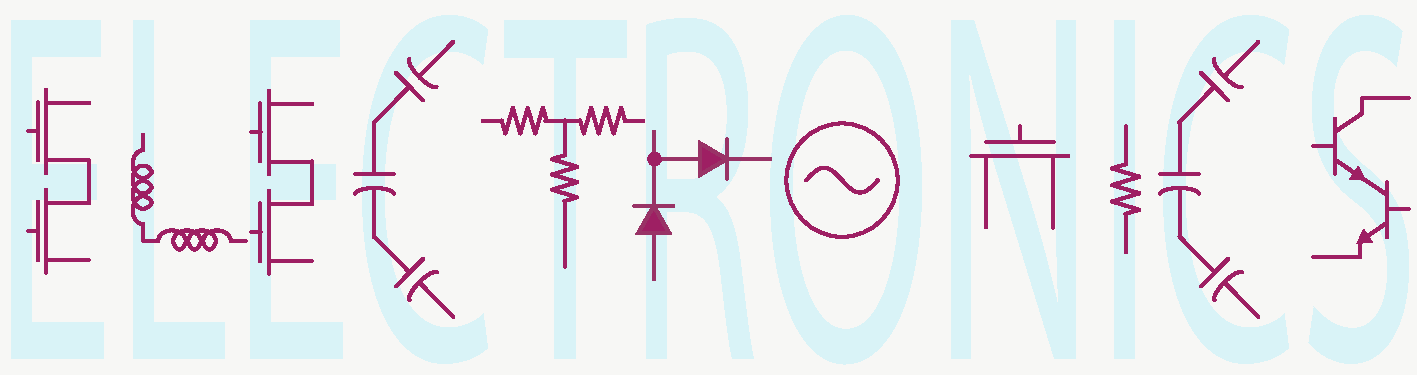
\includegraphics[width=.7\paperwidth]{edogslogo.pdf}\\
%[15pt] % Book title
{\Large EE105 Reader}\\[20pt] % Subtitle
{\huge Ali M. Niknejad}}}; % Author name
\end{tikzpicture}};
\end{tikzpicture}
\vfill
\endgroup
%----------------------------------------------------------------------------------------
%	COPYRIGHT PAGE
%----------------------------------------------------------------------------------------
\newpage
~\vfill
\thispagestyle{empty}
\noindent Copyright \copyright 2022 Ali Niknejad

\vspace{0.5cm}
\noindent
\textsc{Published by Ali Niknejad}

\vspace{0.5cm}
\noindent
\url{http://rfic.eecs.berkeley.edu/~niknejad/edogs.html}

\vspace{0.5cm}
\noindent
% License information
Licensed under the Creative Commons Attribution-NonCommercial 3.0 Unported License (the ``License''). You may not use this file except in compliance with the License. You may obtain a copy of the License at \url{http://creativecommons.org/licenses/by-nc/3.0}. Unless required by applicable law or agreed to in writing, software distributed under the License is distributed on an \textsc{``as is'' basis, without warranties or conditions of any kind}, either express or implied. See the License for the specific language governing permissions and limitations under the License.

% Printing/edition date
\vspace{0.5cm}
\noindent
\textit{First printing, January 17, 2020}

\vspace{0.5cm}
\noindent
\textit{Latest printing, August 17, 2022}
%----------------------------------------------------------------------------------------
%	TABLE OF CONTENTS
%----------------------------------------------------------------------------------------
\chapterimage{Pictures/lm358.PNG} % Table of contents heading image
\pagestyle{empty} % No headers
\tableofcontents % Print the table of contents itself
\cleardoublepage % Forces the first chapter to start on an odd page so it's on the right
\pagestyle{fancy} % Print headers again
%----------------------------------------------------------------------------------------
%	CHAPTERS
%----------------------------------------------------------------------------------------
\chapterimage{Pictures/logo105.pdf} % Chapter heading image
%%!TEX root = edance.tex
%%%%%%%%%%%%%%%%
%   CHAPTER 1  %
%%%%%%%%%%%%%%%%
\chapter{Linear Time-Invariant Systems}
\label{ch:ch01_LTI}
\graphicspath{{./figs_LTI/}}
%%%%%%%%%%%%%%%%%%%%%%%%%%%%%%%%%%%%%%%%%%%%%%%%%%%%%%%%%%%%%%%%%%%%%%%%%%%%%%%%%%%%%%%%
%%%%%%%%%%%%%%%%%%%%%%%%%%%%%%%%%%%%%%%%%%%%%%%%%%%%%%%%%%%%%%%%%%%%%%%%%%%%%%%%%%%%%%%%
%                                   SECTION 1.1                                        %
%%%%%%%%%%%%%%%%%%%%%%%%%%%%%%%%%%%%%%%%%%%%%%%%%%%%%%%%%%%%%%%%%%%%%%%%%%%%%%%%%%%%%%%%
%%%%%%%%%%%%%%%%%%%%%%%%%%%%%%%%%%%%%%%%%%%%%%%%%%%%%%%%%%%%%%%%%%%%%%%%%%%%%%%%%%%%%%%%
\section{Chapter Preview}
In this chapter we will review linearity in the context of an Linear Time-Invariant (LTI) system by making analogies with discrete finite dimensional systems.  Many people have familiarity with concepts such as orthogonality and eigenfunctions from linear algebra.  It's not critical to have this background, so these references can be skipped.  Most importantly, we will show that complex exponential functions are eigenfunctions of linear systems and they span the space of solutions.  We will define the time-domain impulse response and convolution operator, and in a very natural way show the relation between the impulse response and the transfer function in the frequency domain.  This will lead us into a preview of the frequency domain representation of linear systems, which we'll pick up in the next chapter.
%%%%%%%%%%%%%%%%%%%%%%%%%%%%%%%%%%%%%%%%%%%%%%%%%%%%%%%%%%%%%%%%%%%%%%%%%%%%%%%%%%%%%%%%
%%%%%%%%%%%%%%%%%%%%%%%%%%%%%%%%%%%%%%%%%%%%%%%%%%%%%%%%%%%%%%%%%%%%%%%%%%%%%%%%%%%%%%%%
%                                   SECTION 1.2                                        %
%%%%%%%%%%%%%%%%%%%%%%%%%%%%%%%%%%%%%%%%%%%%%%%%%%%%%%%%%%%%%%%%%%%%%%%%%%%%%%%%%%%%%%%%
%%%%%%%%%%%%%%%%%%%%%%%%%%%%%%%%%%%%%%%%%%%%%%%%%%%%%%%%%%%%%%%%%%%%%%%%%%%%%%%%%%%%%%%%
\section{Example:  Analyzing an RLC Circuit}
%%%%%%%%%%%%%%%%%%%%%%%%%%%%%%%%%%%%%%%%%%%%
%             SUBSECTION 1.2.1             %
%%%%%%%%%%%%%%%%%%%%%%%%%%%%%%%%%%%%%%%%%%%%
\subsection{Example:  Low Pass Filter (LPF)}
Let's begin with an example calculation.  Suppose we have a \textbf{low pass filter}\index{Filters!Low pass} as shown in \emph{Fig.~\ref{fig:lpf}}.
%%%%%%%%%%%%%%%%%%%%%%%%%%%%%%%%%%%%%%%%%%%%
%                 FIGURE                   %
%%%%%%%%%%%%%%%%%%%%%%%%%%%%%%%%%%%%%%%%%%%%
\begin{figure}[tb]
\centering
\includegraphics[scale=1]{lpf}
\caption{A simple $RC$ low-pass filter.}
\label{fig:lpf}
\end{figure}
%%%%%%%%%%%%%%%%%%%%%%%%%%%%%%%%%%%%%%%%%%%%
If we drive this system with a source $v_s$ and observe the output at $v_o$, we can write the governing equations as follows by using KVL around the loop:
    \begin{align*}
        v_o(t) &= v_s(t) - v_r(t)\\
        &= v_s(t) - i(t) R
    \end{align*}
Recall the current in a capacitor:
    \begin{equation}
        i(t) = C \frac{dv_c(t)}{dt} \label{eq:cap_curr}
    \end{equation}
Since the current is the same through the resistor and capacitor, and the voltage at the output is the same as the voltage across the capacitor, we have:
    \begin{equation*}
        v_o(t) = v_s(t) - RC \frac{dv_o(t)}{dt}
    \end{equation*}
Or, in terms of the circuit time constant $\tau = RC$:
    \begin{equation}
        v_o(t) = v_s(t) - \tau \frac{dv_o(t)}{dt} \label{eq:lpf_diff}
    \end{equation}
Let's suppose that the input signal is given by $v_s(t) = V_s \cos(\omega t)$.  We know that in steady-state  the output amplitude and phase will change: 
    \begin{equation}
        v_o(t) = \underbrace{K \cdot V_s}_{V_o} \cos(\omega t + \phi) \label{eq:kvl1}
    \end{equation}  
How do we find the change in the amplitude and phase of the signal?
%%%%%%%%%%%%%%%%%%%%%%%%%%%%%%%%%%%%%%%%%%%%
%             SUBSECTION 1.2.2             %
%%%%%%%%%%%%%%%%%%%%%%%%%%%%%%%%%%%%%%%%%%%%
\subsection{LPF the ``hard way"}
The following is the wrong way to solve the problem.  It's important to review it to see how painful it can be even for a simple example.  We start by plugging the known form of the output(\emph{Eq.~\ref{eq:kvl1}}) into the LHS of the governing equation(\emph{Eq.~\ref{eq:lpf_diff}}), and verify that it satisfies the equation:
    \begin{align*}
        V_o \cos(\omega t + \phi) &= v_s(t) - \tau \frac{d}{dt}\bigg( v_o(t) \bigg)\\
        &= V_s \cos(\omega t) - \tau \frac{d}{dt}\bigg( V_o \cos(\omega t + \phi) \bigg)
            &\text{\emph{Substituting for $v_s(t)$ and $v_o(t)$}}\\
        &= V_s \cos(\omega t) + \tau \omega V_o \sin(\omega t + \phi)
    \end{align*}
Rearranging, we have:
    \begin{equation}
        V_s \cos(\omega t) = V_o \cos(\omega t + \phi) - \tau \omega V_o \sin(\omega t + \phi) \label{eq:kvl2}
    \end{equation}
Recall the following trigonometric identities:
    \begin{align*}
        \cos(x + y) &= \cos x \cos y - \sin x \sin y &\text{\emph{Sum of angles for cosine}}\\
        \sin(x + y) &= \sin x \cos y + \cos x \sin y &\text{\emph{Sum of angles for sine}}
    \end{align*}
Applying the identities to \emph{Eq.~\ref{eq:kvl2}}:
    \begin{align*}
        V_s \cos(\omega t) &= V_o \big(\cos \omega t \cos \phi - \sin \omega t \sin \phi \big)
            - \tau \omega V_o \big( \sin \omega t \cos \phi + \cos \omega t \sin \phi \big)\\
        &= V_o \cos \omega t \cos \phi - V_o \sin \omega t \sin \phi
            - V_o \tau \omega \sin \omega t \cos \phi + V_o \tau \omega \cos \omega t \sin \phi
    \end{align*}
Factoring, we have:
    \begin{equation}
        V_s \cos(\omega t) = V_o \cos(\omega t) (\cos \phi - \tau \omega \sin\phi) - V_o \sin(\omega t) (\sin\phi + \tau \omega \cos\phi)
    \end{equation}
Since sine and cosine are linearly independent\footnote{See Appendix B for a review of linear dependence/independence, and a proof for sine and cosine are LI.} functions:
    \begin{equation}
        a_1 \sin(\omega t) + a_2 \cos(\omega t) = 0
    \end{equation}
This implies that $a_1 = 0$ and $a_2 = 0$ must be zero independently.  Applying the linear independence gives us
    \begin{equation}
        -V_o \sin\phi - V_o \tau \omega \cos \phi = 0
    \end{equation}
and
    \begin{equation}
        \tan \phi = -\tau \omega
    \end{equation}
The phase response is therefore 
    \begin{equation}
        \phi = - \tan^{-1} \tau \omega
    \end{equation}
Likewise we have
    \begin{equation}
        V_o \cos\phi - V_o \tau \omega \sin\phi - V_s = 0
    \end{equation}
    \begin{equation}
        V_o (\cos \phi - \tau \omega \sin\phi) = V_s
    \end{equation}
    \begin{equation}
        V_o \cos \phi (1  - \tau \omega \tan\phi) = V_s
    \end{equation}
    \begin{equation}
        V_o \cos \phi (1  + (\tau \omega)^2 ) = V_s
    \end{equation}
    \begin{equation}
        V_o (1  + (\tau \omega)^2 )^{1/2} = V_s
    \end{equation}
 The amplitude response is therefore given by
    \begin{equation}
        \frac{V_o}{V_s} = \frac{1}{\sqrt{1 + (\tau \omega)^2}}
    \end{equation}
We can see that both the \textbf{amplitude}\index{Filters!amplitude} and \textbf{phase response}\index{Filters!phase response} are a strong function of frequency.  At very low frequencies, $\omega \approx 0$, the signal passes undisturbed.  At very high frequencies $\omega \rightarrow \infty$, the signal experiences infinite attenuation and is effectively shorted out by the capacitor.
\newpage
%%%%%%%%%%%%%%%%%%%%%%%%%%%%%%%%%%%%%%%%%%%%
%              SUB-SUBSECTION              %
%%%%%%%%%%%%%%%%%%%%%%%%%%%%%%%%%%%%%%%%%%%%
\subsubsection{LPF Magnitude and Phase Response}
%%%%%%%%%%%%%%%%%%%%%%%%%%%%%%%%%%%%%%%%%%%%
Plots of the magnitude and phase response are shown in \emph{Fig.~\ref{fig:magphase}}.  The magnitude plot shows that for signal frequencies below the cutoff frequency, $1/\tau$, the signal experiences little attenuation.  In fact, at the passband edge frequency of $1/\tau$, the magnitude is by definition lower by $1/\sqrt{2}$, which corresponds to half the power.  Likewise, the phase response is zero at low frequencies, meaning the signal is not delayed, but even at the cutoff frequency the delay is $45^\circ$, and asymptotically reaches $90^\circ$.

As is common practice in electrical engineering, we more often plot the magnitude on a log-log scale with units of dB,  as shown in \emph{Fig.~\ref{fig:magphase}}.  On the deciBel (deci = 10) scale, we take the base 10 $\log_{10}$ and multiply by $10$ to get rid of fractional parts.  The "Bel" part is in honor of the inventor of the phone,.  The dB scale allows us to expand the passband and more clearly understand the behavior of the transfer function as a function of frequency.  The multiplication by 10 is just for convenience.

But you'll notice that we often multiply log by $20$ rather than $10$ in the definition of $dB$.  Why is that?  Remember that power is proportional to voltage squared\footnote{See Appendix~\ref{sec:power_decibel} for a review of power and decibel conversions.}:
    \begin{equation}
        \mathrm{dB} = 10 \log\left( \frac{V_o}{V_s} \right)^2 = 20 \log\left( \frac{V_o}{V_s} \right)
    \end{equation}
which means that if we take the $\log$ of voltage, we can just multiply by 2 o convert it into power.
At various frequencies we have:
    \begin{equation}
        \omega = 1/\tau \rightarrow \left( \frac{V_o}{V_s} \right)_{\mathrm{dB}} = -3 \mathrm{dB}
    \end{equation}
    \begin{equation}
        \omega = 100/\tau \rightarrow \left( \frac{V_o}{V_s} \right)_{\mathrm{dB}} = -40 \mathrm{dB}
    \end{equation}
    \begin{equation}
        \omega = 1000/\tau \rightarrow \left( \frac{V_o}{V_s} \right)_{\mathrm{dB}} = -60 \mathrm{dB}
    \end{equation}
Observe that the slope of signal attenuation is 20 dB/decade in frequency beyond the passband.   Alternatively, if you double the frequency, the attenuation changes by 6 dB, or 6 dB/decade.  This is an important rule of thumb when understanding the frequency response of a system.
\newpage
%%%%%%%%%%%%%%%%%%%%%%%%%%%%%%%%%%%%%%%%%%%%
%                 FIGURE                   %
%%%%%%%%%%%%%%%%%%%%%%%%%%%%%%%%%%%%%%%%%%%%
\begin{figure}[H]
\centering
\begin{tabular}{c}
\includegraphics[width=.65\columnwidth]{mag}\\
(a)\\
\includegraphics[width=.65\columnwidth]{phase}\\
(b)\\
\includegraphics[width=.65\columnwidth]{dB}\\
(c)\\
\end{tabular}
\caption{The (a) magnitude and (b) phase response of the low-pass filter. The (c) log-log plot of the magnitude response of a low-pass filter (dB scale).}
\label{fig:magphase}
\end{figure}
\newpage
%%%%%%%%%%%%%%%%%%%%%%%%%%%%%%%%%%%%%%%%%%%%%%%%%%%%%%%%%%%%%%%%%%%%%%%%%%%%%%%%%%%%%%%%
%%%%%%%%%%%%%%%%%%%%%%%%%%%%%%%%%%%%%%%%%%%%%%%%%%%%%%%%%%%%%%%%%%%%%%%%%%%%%%%%%%%%%%%%
%                                   SECTION 1.3                                        %
%%%%%%%%%%%%%%%%%%%%%%%%%%%%%%%%%%%%%%%%%%%%%%%%%%%%%%%%%%%%%%%%%%%%%%%%%%%%%%%%%%%%%%%%
%%%%%%%%%%%%%%%%%%%%%%%%%%%%%%%%%%%%%%%%%%%%%%%%%%%%%%%%%%%%%%%%%%%%%%%%%%%%%%%%%%%%%%%%
\section{Linear Time-Invariant Systems}
%%%%%%%%%%%%%%%%%%%%%%%%%%%%%%%%%%%%%%%%%%%%
%             SUBSECTION 1.3.1             %
%%%%%%%%%%%%%%%%%%%%%%%%%%%%%%%%%%%%%%%%%%%%
\subsection{Linear Time-Invariant Definition}
A system $\mathbf{L}$ is linear if it satisfies the following requirement:
    \begin{equation}
        \mathbf{L} [ \alpha x(t) + \beta y(t) ] = \alpha \mathbf{L}[ x(t) ] + \beta \mathbf{L}[ y(t) ]
    \end{equation}
In this notation, $\mathbf{L}$ is an operator that corresponds to the action of the system at hand. If we input $x(t)$ an input into our system, the system outputs $y(t)$.  In a \textbf{linear system}\index{Linear systems}, if we scale the input, we also scale the output by the same amount. Also, if we take a superposition of inputs, the output is the same superposition of the inputs.

Now, a system is \textbf{time invariant}\index{Linear systems!Time invariant} if its response is not a function of time. In other words, the system does not "age" and it does not care when you apply the input.  If you apply an input today and observe the output, and come back tomorrow and put in the same input, the output should look the same.  Mathematically, we can summarize this behavior with the following equations:
    \begin{equation}
        y(t) = \mathbf{L} [x(t)]
    \end{equation}
    \begin{equation}
        \mathbf{L} [x(t-\tau)] = y(t-\tau)
    \end{equation}
Notice that \textbf{time shifting}\index{Linear systems!Time shifting} the input just corresponds to applying the same time shift to the output.  Another way to think of time-invariance is to say that the system has no  ``clock" or time reference, or that the transfer function is not a function of time.  It does not matter when you apply the input.  The transfer function is going to be the same. 

 If you are familiar with discrete linear system, you know that linearity and superposition are fundamental properties. 
%%%%%%%%%%%%%%%%%%%%%%%%%%%%%%%%%%%%%%%%%%%%
%              SUB-SUBSECTION              %
%%%%%%%%%%%%%%%%%%%%%%%%%%%%%%%%%%%%%%%%%%%%
\subsubsection{Vectors and Matrices Become Functions and Integrals}
 In finite dimensional discrete linear systems, inputs and outputs are defined in terms of input and output vectors.  For LTI systems, we can think of the inputs and outputs as infinite dimensional vectors, but instead of a countably infinite set of elements we have a uncountably large number of time instants that define the input and output.  In other words, we represent the input and output as continuous functions of time.   We will see that in LTI systems, we can also represent linear systems by basis functions:
    \begin{equation}
        \phi_1(t), \phi_2(t), \cdots
    \end{equation}
and instead of a matrix representation (summation) we will have an integral representation called the \textbf{Convolution Integral}\index{Convolutions!integral}.  Eigenvectors have the direct analog of Eigenfunctions:
    \begin{equation}
        \mathbf{L} [  \phi_n(t)  ] = \lambda_n  \phi_n(t)
    \end{equation}
And the concept of an \textbf{Orthonormal Basis}\index{Orthonormal basis} maps directly into LTI systems:
    \begin{equation}
        x(t) = \sum_n \phi_n(t) x_n
    \end{equation}
    \begin{equation}
        x(t) = \int \phi(s t) x(t) dt
    \end{equation}
We can therefore perform \textbf{Eigenfunction}\index{Eigenfunction} expansion of an arbitrary input and study the response of a linear system to an arbitrary input by using our knowledge of how the system responds to the eigenfunctions.  In other words, the eigenvalues of the system, or the spectral expansion, will be the most important aspect of a linear system.

If this doesn't make any sense, don't worry.  We'll cover all of this in a step-by-step fashion. This is only meant as a teaser for people who have seen linear system theory previously. 
%%%%%%%%%%%%%%%%%%%%%%%%%%%%%%%%%%%%%%%%%%%%%%%%%%%%%%%%%%%%%%%%%%%%%%%%%%%%%%%%%%%%%%%%
%%%%%%%%%%%%%%%%%%%%%%%%%%%%%%%%%%%%%%%%%%%%%%%%%%%%%%%%%%%%%%%%%%%%%%%%%%%%%%%%%%%%%%%%
%                                   SECTION 1.4                                        %
%%%%%%%%%%%%%%%%%%%%%%%%%%%%%%%%%%%%%%%%%%%%%%%%%%%%%%%%%%%%%%%%%%%%%%%%%%%%%%%%%%%%%%%%
%%%%%%%%%%%%%%%%%%%%%%%%%%%%%%%%%%%%%%%%%%%%%%%%%%%%%%%%%%%%%%%%%%%%%%%%%%%%%%%%%%%%%%%%
\section{The Complex Exponential Technique}
We begin by introducing the complex exponential, and we will show that complex exponentials are eigenfunctions of linear systems.  This means that they play an immensely central role in linear system analysis.
%%%%%%%%%%%%%%%%%%%%%%%%%%%%%%%%%%%%%%%%%%%%
%             SUBSECTION 1.4.1             %
%%%%%%%%%%%%%%%%%%%%%%%%%%%%%%%%%%%%%%%%%%%%
\subsection{Why introduce complex numbers?}
Complex exponentials actually make things less complex.  To see this, first note that integration and differentiation are trivial with complex exponentials:
    \begin{equation}
        \frac{d}{dt} e^{j\omega t} = j \omega e^{j\omega t}
    \end{equation}
    \begin{equation}
        \int e^{j\omega x} dx = \frac{1}{j \omega} e^{j\omega t}
    \end{equation}
So now any ordinary \textbf{differential equation}\index{Differential equations!ordinary} (ODE), a sum of differentiation operators, is reduced now to trivial algebraic manipulations.  In fact, we'll show that you don't even need to directly derive the ODE by using \textbf{phasors}\index{Phasors} (a phasor is essentially a shorthand notation for a complex number).   The key is to observe that the current/voltage relation for any element can be derived for \textbf{complex exponential}\index{Complex exponential} excitation.
%%%%%%%%%%%%%%%%%%%%%%%%%%%%%%%%%%%%%%%%%%%%
%             SUBSECTION 1.4.2             %
%%%%%%%%%%%%%%%%%%%%%%%%%%%%%%%%%%%%%%%%%%%%
\subsection{Complex Exponential}
From Euler's we have an important relationship between complex exponentials and ordinary $\sin$ and $\cos$ functions:
    \begin{equation}
        e^{j x} = \cos x + j \sin x
    \end{equation}
If take the magnitude of this quantity, it's unity
    \begin{equation}
        | e^{j x} | = \sqrt{\cos^2 x +  \sin^2 x}  = 1
    \end{equation}
This means that for any value of $x$, the magnitude of a complex exponential is 1.  Thus,  $e^{j\phi}$ is a point on the unit circle at an angle of $\phi$ from the $x$-axis. 

Any complex number $z$ (\emph{Fig.~\ref{fig:complex}}), expressed as having a real and imaginary part $ z = x + j y$, can also be interpreted as having a magnitude and a phase.  The magnitude  $|z| = \sqrt{x^2 + y^2}$ and the phase $\phi = \angle z = \tan^{-1} y/x$ can be combined using the complex exponential
    \begin{equation}
        x + j y = |z| e^{j\phi}
    \end{equation}
%%%%%%%%%%%%%%%%%%%%%%%%%%%%%%%%%%%%%%%%%%%%
%                 FIGURE                   %
%%%%%%%%%%%%%%%%%%%%%%%%%%%%%%%%%%%%%%%%%%%%
\begin{figure}[H]
\centering
\includegraphics[width=.55\columnwidth]{complex}
\caption{A general complex number $z$ can be represented by its real and imaginary components, or its magnitude and phase.}
\label{fig:complex}
\end{figure}
%%%%%%%%%%%%%%%%%%%%%%%%%%%%%%%%%%%%%%%%%%%%
%%%%%%%%%%%%%%%%%%%%%%%%%%%%%%%%%%%%%%%%%%%%
%             SUBSECTION 1.4.3             %
%%%%%%%%%%%%%%%%%%%%%%%%%%%%%%%%%%%%%%%%%%%%
\subsection{Euler's Relations and The Circle}
The argument to $e^{j \omega t}$ is just linearly increasing with a slope of $\omega$, and completes $2\pi$ radian every $\frac{2\pi}{\omega}$ seconds.  This implies that $e^{j \omega t}$ is nothing but a point rotating on a circle on the complex plane.  The real part and imaginary parts are just projections of the circle, which by trigonometry we know equal the cosine and sine functions.

 We can also express $\cos$ and $\sin$ in terms of $e$ as follows
    \begin{equation}
        \cos x = \frac{e^{jx} + e^{-jx}}{2}
    \end{equation}
    \begin{equation}
        \sin x = \frac{e^{jx} - e^{-jx}}{2j}
    \end{equation}
which shows that two counter rotating complex exponentials sum to $\sin$ and $\cos$.  We can visualize these relations as shown in \emph{Fig.~\ref{fig:complexexp}}.  Be sure to click the links to see an animation, especially for the sum of two counter rotating complex exponentials in \emph{Fig.~\ref{fig:cos}}.
%%%%%%%%%%%%%%%%%%%%%%%%%%%%%%%%%%%%%%%%%%%%
%                 FIGURE                   %
%%%%%%%%%%%%%%%%%%%%%%%%%%%%%%%%%%%%%%%%%%%%
\begin{figure}[tb]
\centering
\begin{tabular}{cc}
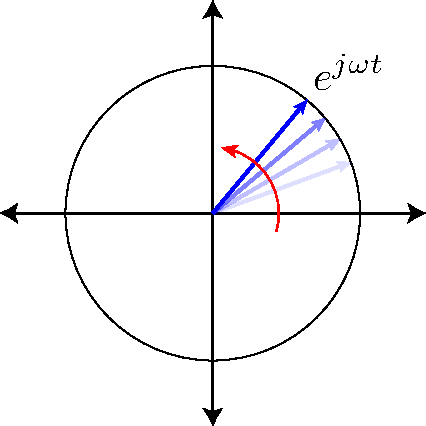
\includegraphics[width=.4\columnwidth]{exp1.pdf}  &
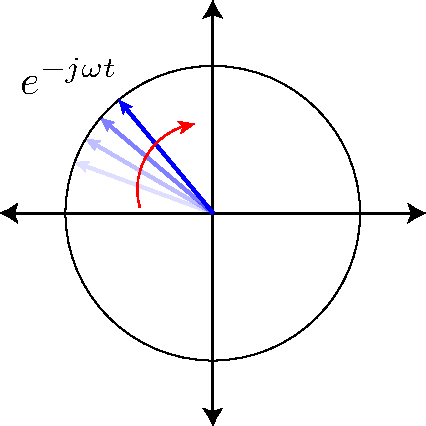
\includegraphics[width=.4\columnwidth]{exp2.pdf} \\
(a) & (b) \\
\end{tabular}
\caption{  (a) The complex exponential $e^{j\omega t}$ rotates around the unit circle counter-clockwise at a rate of $\omega$, or once every $2\pi/\omega$ seconds.  Likewise (b) $e^{-j\omega t}$ rotates around the unit circle clockwise.  Click \href{http://rfic.eecs.berkeley.edu/~niknejad/photos/ee105/exp1.mov}{$e^{j\omega t}$ \emph{here}} and \href{http://rfic.eecs.berkeley.edu/~niknejad/photos/ee105/exp2.mov}{$e^{-j\omega t}$ \emph{here}} to see the animations.}
\label{fig:complexexp}
\end{figure}
%%%%%%%%%%%%%%%%%%%%%%%%%%%%%%%%%%%%%%%%%%%%
%                 FIGURE                   %
%%%%%%%%%%%%%%%%%%%%%%%%%%%%%%%%%%%%%%%%%%%%
\begin{figure}[tb]
\centering
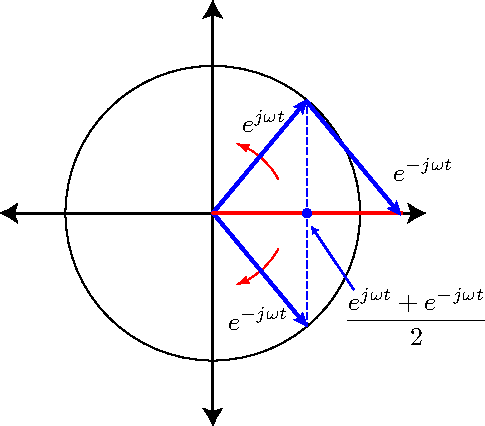
\includegraphics[width=.45\columnwidth]{exp3.pdf}
\caption{We visualize the function $\cos$ by building it through vectorwise addition of $e^{j\omega t}$ and $e^{-j\omega t}$.  Click \href{http://rfic.eecs.berkeley.edu/~niknejad/photos/ee105/exp3.mov}{\emph{here}} to see the animation.}
\label{fig:cos}
\end{figure}
%%%%%%%%%%%%%%%%%%%%%%%%%%%%%%%%%%%%%%%%%%%%
%             SUBSECTION 1.4.4             %
%%%%%%%%%%%%%%%%%%%%%%%%%%%%%%%%%%%%%%%%%%%%
\subsection{The Magic of Sinusoids}
%%%%%%%%%%%%%%%%%%%%%%%%%%%%%%%%%%%%%%%%%%%%
%                 FIGURE                   %
%%%%%%%%%%%%%%%%%%%%%%%%%%%%%%%%%%%%%%%%%%%%
\begin{figure}[tb]
\centering
\includegraphics[width=.65\columnwidth]{lti_sine}
\caption{In an LTI system, if we drive it with a sinusoid, the output is a sinusoid at the same frequency, with a new amplitude and phase.}
\label{fig:lti_sine}
\end{figure}
%%%%%%%%%%%%%%%%%%%%%%%%%%%%%%%%%%%%%%%%%%%%
What were going to show is that when a linear, time invariant (LTI) circuit is excited by a sinusoid (see \emph{Fig.~\ref{fig:lti_sine}}), it's output is a sinusoid at the same frequency.  Only the magnitude and phase of the output differ from the input.  Sinusoids are very special functions for LTI systems, in other words they are eigenfunctions.  The \textbf{``Frequency Response''}\index{Linear systems!frequency response} is a characterization of the input-output response for sinusoidal inputs at all frequencies.

Since most periodic (non-periodic) signals can be decomposed into a summation (integration) of sinusoids via Fourier Series (Transform), the response of a LTI system to virtually any input is characterized by the frequency response of the system.  We'll return to this point later.
%%%%%%%%%%%%%%%%%%%%%%%%%%%%%%%%%%%%%%%%%%%%
%              SUB-SUBSECTION              %
%%%%%%%%%%%%%%%%%%%%%%%%%%%%%%%%%%%%%%%%%%%%
\subsubsection{Complex Exponential is Powerful}
To find steady state response we can excite the system with a complex exponential.   Here our system is any general LTI system. In terms of circuits, it is any linear circuit consisting of resistors, capacitors, inductors, mutual inductors, transformers, and linear dependent sources.  At any frequency, the system response is characterized by a single complex number $H$, as shown in \emph{Fig.~\ref{fig:lti_resp}}.   The magnitude response is given by $|H(\omega)|$ and
the phase response is given by $\angle H$.   We see that the complex exponential is an ``eigenfunction" of the system.  It is used to probe the system.  If we characterize the response to all eigenfunctions, we can completely characterize the system.   Because a sinusoid is a sum of complex exponentials (and because of linearity!), we can also probe a system by applying a real sinusoidal input.  This is what we do in the lab.
%%%%%%%%%%%%%%%%%%%%%%%%%%%%%%%%%%%%%%%%%%%%
%                 FIGURE                   %
%%%%%%%%%%%%%%%%%%%%%%%%%%%%%%%%%%%%%%%%%%%%
\begin{figure}[tb]
\centering
\includegraphics[width=.65\columnwidth]{lti_resp}
\caption{The complex exponential response of a linear system is another complex exponential, with an additional magnitude and phase factor. }
\label{fig:lti_resp}
\end{figure}
%%%%%%%%%%%%%%%%%%%%%%%%%%%%%%%%%%%%%%%%%%%%
%              SUB-SUBSECTION              %
%%%%%%%%%%%%%%%%%%%%%%%%%%%%%%%%%%%%%%%%%%%%
\subsubsection{$H$ is the Transfer Function}
In summary, $e^{j\omega}$ is an eigenfunction for any linear system (circuit), and $H(\omega)$ is the eigenvalue of the system.  There's a continuous spectrum of eigenvalues $H(\omega)$.   The linear system is completely characterized by the spectrum of eigenvalues, or in the frequency domain by the \textbf{transfer function}\index{Transfer function} $H(\omega)$.  We also often write $H(\omega)$ in the following form (explained shortly):
    \begin{equation}
        H(j\omega)
    \end{equation}
%%%%%%%%%%%%%%%%%%%%%%%%%%%%%%%%%%%%%%%%%%%%%%%%%%%%%%%%%%%%%%%%%%%%%%%%%%%%%%%%%%%%%%%%
%%%%%%%%%%%%%%%%%%%%%%%%%%%%%%%%%%%%%%%%%%%%%%%%%%%%%%%%%%%%%%%%%%%%%%%%%%%%%%%%%%%%%%%%
%                                   SECTION 1.5                                        %
%%%%%%%%%%%%%%%%%%%%%%%%%%%%%%%%%%%%%%%%%%%%%%%%%%%%%%%%%%%%%%%%%%%%%%%%%%%%%%%%%%%%%%%%
%%%%%%%%%%%%%%%%%%%%%%%%%%%%%%%%%%%%%%%%%%%%%%%%%%%%%%%%%%%%%%%%%%%%%%%%%%%%%%%%%%%%%%%%
\section{The Low Pass Filter Again}
%%%%%%%%%%%%%%%%%%%%%%%%%%%%%%%%%%%%%%%%%%%%
%             SUBSECTION 1.5.1             %
%%%%%%%%%%%%%%%%%%%%%%%%%%%%%%%%%%%%%%%%%%%%
\subsection{LPF Example:  The ``soft way''}
Remember that earlier we tried to analyze the low-pass filter using sinusoids.  Now let's excite the system with a complex exponential.  Recall that the sinusoidal response is related to the exponential response so we can always recover the sinusoidal response from the complex exponential\index{Complex exponential} response
    \begin{equation}
        v_s(t) = v_o(t) + \tau \frac{dv_o}{dt}
    \end{equation}
Derivatives are simply products with $j\omega$
    \begin{equation}
        v_s(t) = V_s e^{j\omega t}
    \end{equation}
Grouping terms
    \begin{equation}
        v_o(t) = |V_o| e^{j (\omega t + \phi)} = V_o e^{j\omega t}
    \end{equation}
Now substitute into the original equation
    \begin{equation}
        V_s e^{j \omega t} = V_o e^{j \omega t}  + \tau \cdot j\omega \cdot V_o e^{j \omega t}
    \end{equation}
and divide out the non-zero common factors ($|e^{j\omega t} | = 1$)
    \begin{equation}
        V_s = V_o ( 1 + j \omega \cdot \tau)
    \end{equation}
So with a few lines of algebra, we have the transfer function:
    \begin{equation}
        \frac{V_o}{V_s} = \frac{1}{1 + j\omega \cdot \tau}
    \end{equation}
The system is characterized by the complex function
    \begin{equation}
        H(\omega) = \frac{V_o}{V_s} = \frac{1}{1 + j\omega \cdot \tau}
    \end{equation}
The magnitude and phase response match our previous calculation:
    \begin{equation}
        | H(\omega) | = \left|\frac{V_o}{V_s}\right| = \frac{1}{\sqrt{1 + (\omega \tau)^2}}
    \end{equation}
    \begin{equation}
        \angle H(\omega) = - \tan^{-1} \omega \tau
    \end{equation}
Clearly, using the complex exponential is much faster and easier than the earlier approach where we used sinusoids directly and the final answer is the same.  It's not obvious why the transfer function for a complex exponential matches the one for the sinusoidal excitation.  Let's explore this further.
%%%%%%%%%%%%%%%%%%%%%%%%%%%%%%%%%%%%%%%%%%%%
%              SUB-SUBSECTION              %
%%%%%%%%%%%%%%%%%%%%%%%%%%%%%%%%%%%%%%%%%%%%
\subsubsection{Why did it work?}
If we push the complex exponential through the system and take the real part of the output, then why is that the same as the ``real'' sinusoidal response?  One argument to explain why the complex exponential works in place of a sinusoid is to observe that sine and cosine are simply imaginary and real parts of the complex exponential.  So any signal (current or voltage) can be written in the following equivalent forms
    \begin{equation}
        s(t) = S_o \cos(\omega t + \phi) = S_o \Re[e^{j(\omega t + \phi)}]
    \end{equation}
For example, if we excite our system with an input $z(t)$ that is complex, producing an output $y_z(t)$, and if we take the real or imaginary part of the signals, we have
    \begin{equation}
        y_z(t) = \mathbf{L}(z(t))
    \end{equation}
Now take the real part of both sides and use the fact that the order of the operator $\Re$ and our system $\mathbf{L}$ can be interchanged:
    \begin{equation}
        \Re[y_z(t)] = \Re[\mathbf{L}(z(t))]  = \mathbf{L} (\Re[z(t)])
    \end{equation}
If this argument does not convince you, there's a slightly more complicated way to show this must be true.
%%%%%%%%%%%%%%%%%%%%%%%%%%%%%%%%%%%%%%%%%%%%
%                 FIGURE                   %
%%%%%%%%%%%%%%%%%%%%%%%%%%%%%%%%%%%%%%%%%%%%
\begin{figure}[tb]
\centering
\includegraphics[width=.75\columnwidth]{lti_cosine}
\caption{Sinusoidal response of an LTI system by superposition. }
\label{fig:lti_cosine}
\end{figure}
%%%%%%%%%%%%%%%%%%%%%%%%%%%%%%%%%%%%%%%%%%%%
%              SUB-SUBSECTION              %
%%%%%%%%%%%%%%%%%%%%%%%%%%%%%%%%%%%%%%%%%%%%
\subsubsection{And yet another perspective}
As shown in \emph{Fig.~\ref{fig:lti_cosine}}, another way to see this is to observe that the system is linear so that we can push through two inputs separately and sum the outputs:
    \begin{equation}
        y = \mathbf{L}(s_1(t) + s_2(t)) = \mathbf{L}(s_1(t)) + \mathbf{L}(s_2(t))
    \end{equation}
Similarly, to find the response to a sinusoid, we can find the response to $e^{j\omega t}$ and $e^{-j\omega t}$, and sum the results.  For a linear system represented by real circuit elements, if  the input is real function of time, the output must also be a real function:
    \begin{equation}
        y(t) = \frac{H(\omega) e^{j\omega t} + H(-\omega) e^{-j\omega t} }{2}
    \end{equation}
The only way for two complex numbers to sum to a real number is if they are complex conjugates.  That means the second term is the conjugate of the first, which implies that
    \begin{equation}
        |H(-\omega)| = |H(\omega)|
    \end{equation}
Or in other words, the magnitude response is an even function of frequency.  Likewise, we have
    \begin{equation}
        \angle H(-\omega) = -\angle H(\omega) = - \phi
    \end{equation}
Or the phase function has to be an odd function of frequency.  Therefore the output is given by
    \begin{equation}
        y(t) = \frac{|H(\omega)|}{2} \left( e^{j(\omega t + \phi)} + e^{-j(\omega t + \phi)} \right)
    \end{equation}
or more simply
    \begin{equation}
        |H(\omega)| \cos(\omega t + \phi)
    \end{equation}
%%%%%%%%%%%%%%%%%%%%%%%%%%%%%%%%%%%%%%%%%%%%%%%%%%%%%%%%%%%%%%%%%%%%%%%%%%%%%%%%%%%%%%%%
%%%%%%%%%%%%%%%%%%%%%%%%%%%%%%%%%%%%%%%%%%%%%%%%%%%%%%%%%%%%%%%%%%%%%%%%%%%%%%%%%%%%%%%%
%                                   SECTION 1.6                                        %
%%%%%%%%%%%%%%%%%%%%%%%%%%%%%%%%%%%%%%%%%%%%%%%%%%%%%%%%%%%%%%%%%%%%%%%%%%%%%%%%%%%%%%%%
%%%%%%%%%%%%%%%%%%%%%%%%%%%%%%%%%%%%%%%%%%%%%%%%%%%%%%%%%%%%%%%%%%%%%%%%%%%%%%%%%%%%%%%%
\section{Generalization to any Linear Circuit}
%%%%%%%%%%%%%%%%%%%%%%%%%%%%%%%%%%%%%%%%%%%%
%             SUBSECTION 1.6.1             %
%%%%%%%%%%%%%%%%%%%%%%%%%%%%%%%%%%%%%%%%%%%%
\subsection{``Proof'' for Linear Systems}
For an arbitrary linear circuit, in other words a black box containing an arbitrary number of inductors, capacitors, resistors, mutual inductors, or linear dependent sources, we can  decompose the system into linear sub-operators, like multiplication by constants, time derivatives, or integrals:
    \begin{equation}
        y = \mathbf{L}(x) = a x + b_1 \frac{d}{dt} x + b_2\frac{d^2}{dt^2} x + \cdots + c_1 \int x + c_2 \iint x + \cdots
    \end{equation}
For a complex exponential input this simplifies to:
    \begin{equation}
        y  = \mathbf{L}(e^{j\omega t}) = a e^{j\omega t} + b_1 \frac{d}{dt} e^{j\omega t} + b_2\frac{d^2}{dt^2} e^{j\omega t} + \cdots + c_1 \int e^{j\omega t} + c_2 \iint e^{j\omega t} + \cdots
    \end{equation}
    \begin{equation}
        y  = a e^{j\omega t} + b_1 j\omega e^{j\omega t} + b_2 ( j\omega)^2 e^{j\omega t} + \cdots + c_1 \frac{e^{j\omega t}}{ j\omega} + c_2 \frac{e^{j\omega t}}{ (j\omega)^2} + \cdots
    \end{equation}
Note that every term is of the form $e^{j\omega t}$ times a constant, which when grouped together gives
    \begin{equation}
        y =  e^{j\omega t} \underbrace{\left(a  + b_1 j\omega  + b_2 ( j\omega)^2 + \cdots + c_1 \frac{1}{ j\omega} + c_2 \frac{1}{ (j\omega)^2}  + \cdots \right)}_{H}
    \end{equation}
We've grouped together all the terms multiplying $e^{j\omega t}$ and note that at a given frequency, they sum to a complex number $H$.    The amplitude of the output is the magnitude of the complex number $H$ and the phase of the output is the phase of the complex number $H$.
    \begin{equation}
        y =  e^{j\omega t} \underbrace{\left(a  + b_1 j\omega + b_2 ( j\omega)^2 + \cdots + \frac{1}{ j\omega} + \frac{1}{ (j\omega)^2}  + \cdots \right)}_{H}
    \end{equation}
Written more compactly, we have
    \begin{equation}
        y = e^{j\omega t} |H(\omega)| e^{j\angle H(\omega)}
    \end{equation}
or equivalently
    \begin{equation}
        \Re[ y ] =  |H(\omega)| \cos ( \omega t + \angle H(\omega))
    \end{equation}
%%%%%%%%%%%%%%%%%%%%%%%%%%%%%%%%%%%%%%%%%%%%
%             SUBSECTION 1.6.2             %
%%%%%%%%%%%%%%%%%%%%%%%%%%%%%%%%%%%%%%%%%%%%
\subsection{General Complex Exponential}
Looking back at our derivation, it's clear that a complex exponential is also an eigenfunction of our system, and the periodic complex exponential is just a special case.  We can make the same argument for a general input of the form $e^{st}$:
    \begin{equation}
        y = \mathbf{L}(x) = a x + b_1 \frac{d}{dt} x + b_2\frac{d^2}{dt^2} x + \cdots + c_1 \int x + c_2 \iint x + \cdots
    \end{equation}
    \begin{equation}
        y =  e^{s t} \underbrace{\left(a + b_1 s  + b_2 s^2  + \cdots + \frac{1}{ s} + \frac{1}{ s^2} + \cdots \right)}_{H(s)}
    \end{equation}
Later we'll see that $H(s)$ can be used to solve a problem involving the \textbf{transient response}\index{Transient response} of a system (response to an initial input) whereas $H(j\omega)$ is used to find the \textbf{steady-state response}\index{Steady-state response} to a sinusoidal input.
%%%%%%%%%%%%%%%%%%%%%%%%%%%%%%%%%%%%%%%%%%%%
%              SUB-SUBSECTION              %
%%%%%%%%%%%%%%%%%%%%%%%%%%%%%%%%%%%%%%%%%%%%
\subsubsection{Complex Plane}
In \emph{Fig.~\ref{fig:splane}} we show the ``s-plane", and the "x" marks on the diagram indicate particular complex values of $s$, and the effect these values have on the shape of the response.  Notice that the real axis corresponds to the exponential envelope growth or decay.  The imaginary axis corresponds to the rate of oscillation.  On the real axis, there's no oscillation at all. On the imaginary axis, there's no decay.  This plot shows that the general exponential $e^{st}$ can represent different kinds of functional behavior including steady-state oscillation (sinusoidal response) and other decaying and growing oscillation amplitudes.
%%%%%%%%%%%%%%%%%%%%%%%%%%%%%%%%%%%%%%%%%%%%
%                 FIGURE                   %
%%%%%%%%%%%%%%%%%%%%%%%%%%%%%%%%%%%%%%%%%%%%
\begin{figure}[tb]
\centering
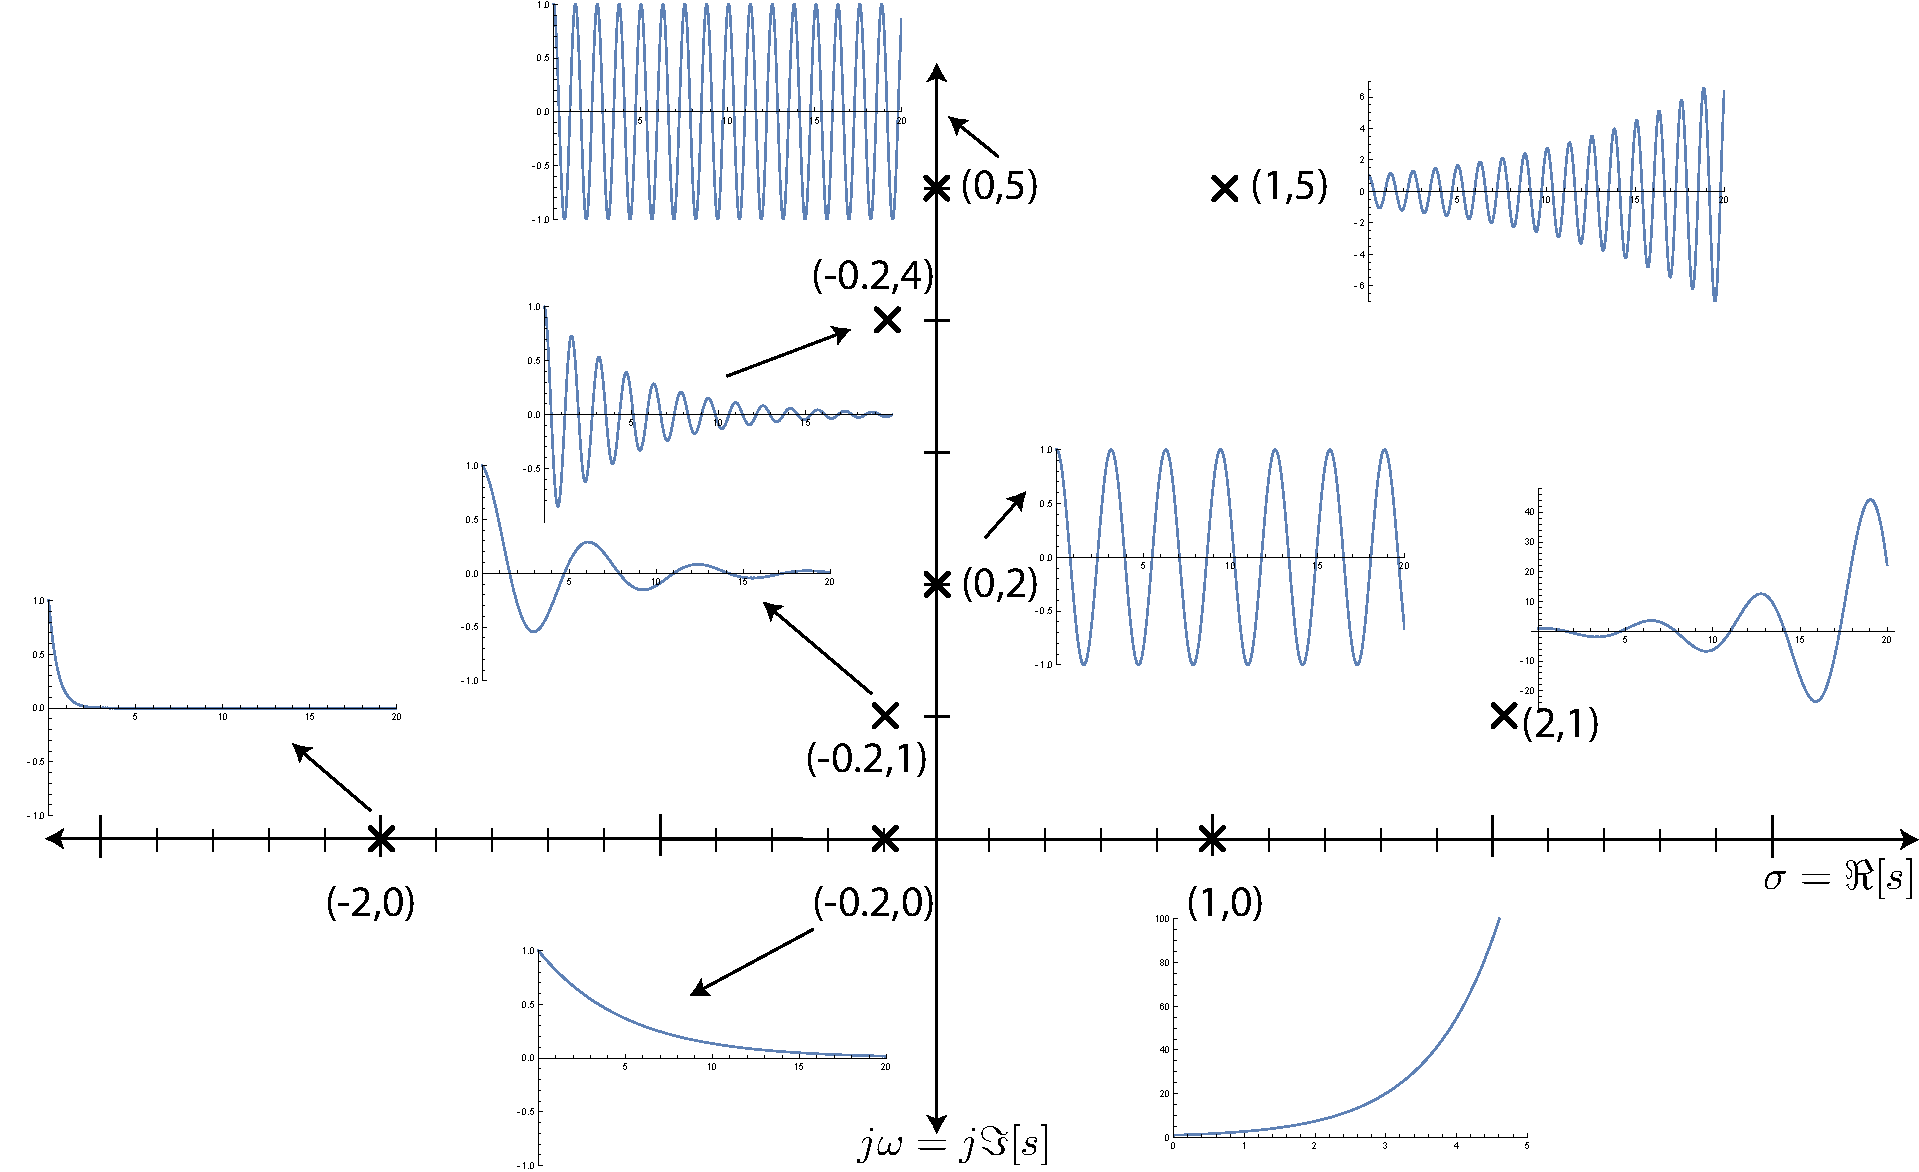
\includegraphics[width=.85\columnwidth]{exp_graph.pdf}
\caption{On the complex plane, the location of the argument $s$ to $e^{st}$ corresponds to either sinusoidal harmonic oscillation (on the imaginary axis), or exponential growth or decay (on the real axis).  Other off-axis locations are a combination of decaying or growing exponential sinusoidal waveforms.}
\label{fig:splane}
\end{figure}
%%%%%%%%%%%%%%%%%%%%%%%%%%%%%%%%%%%%%%%%%%%%%%%%%%%%%%%%%%%%%%%%%%%%%%%%%%%%%%%%%%%%%%%%
%%%%%%%%%%%%%%%%%%%%%%%%%%%%%%%%%%%%%%%%%%%%%%%%%%%%%%%%%%%%%%%%%%%%%%%%%%%%%%%%%%%%%%%%
%                                   SECTION 1.7                                        %
%%%%%%%%%%%%%%%%%%%%%%%%%%%%%%%%%%%%%%%%%%%%%%%%%%%%%%%%%%%%%%%%%%%%%%%%%%%%%%%%%%%%%%%%
%%%%%%%%%%%%%%%%%%%%%%%%%%%%%%%%%%%%%%%%%%%%%%%%%%%%%%%%%%%%%%%%%%%%%%%%%%%%%%%%%%%%%%%%
\section{Time Domain Characterization of Linear Systems}
%%%%%%%%%%%%%%%%%%%%%%%%%%%%%%%%%%%%%%%%%%%%
%             SUBSECTION 1.7.1             %
%%%%%%%%%%%%%%%%%%%%%%%%%%%%%%%%%%%%%%%%%%%%
\subsection{Unit Area Rectangular Function}
%%%%%%%%%%%%%%%%%%%%%%%%%%%%%%%%%%%%%%%%%%%%
%                 FIGURE                   %
%%%%%%%%%%%%%%%%%%%%%%%%%%%%%%%%%%%%%%%%%%%%
\begin{figure}[tb]
\centering
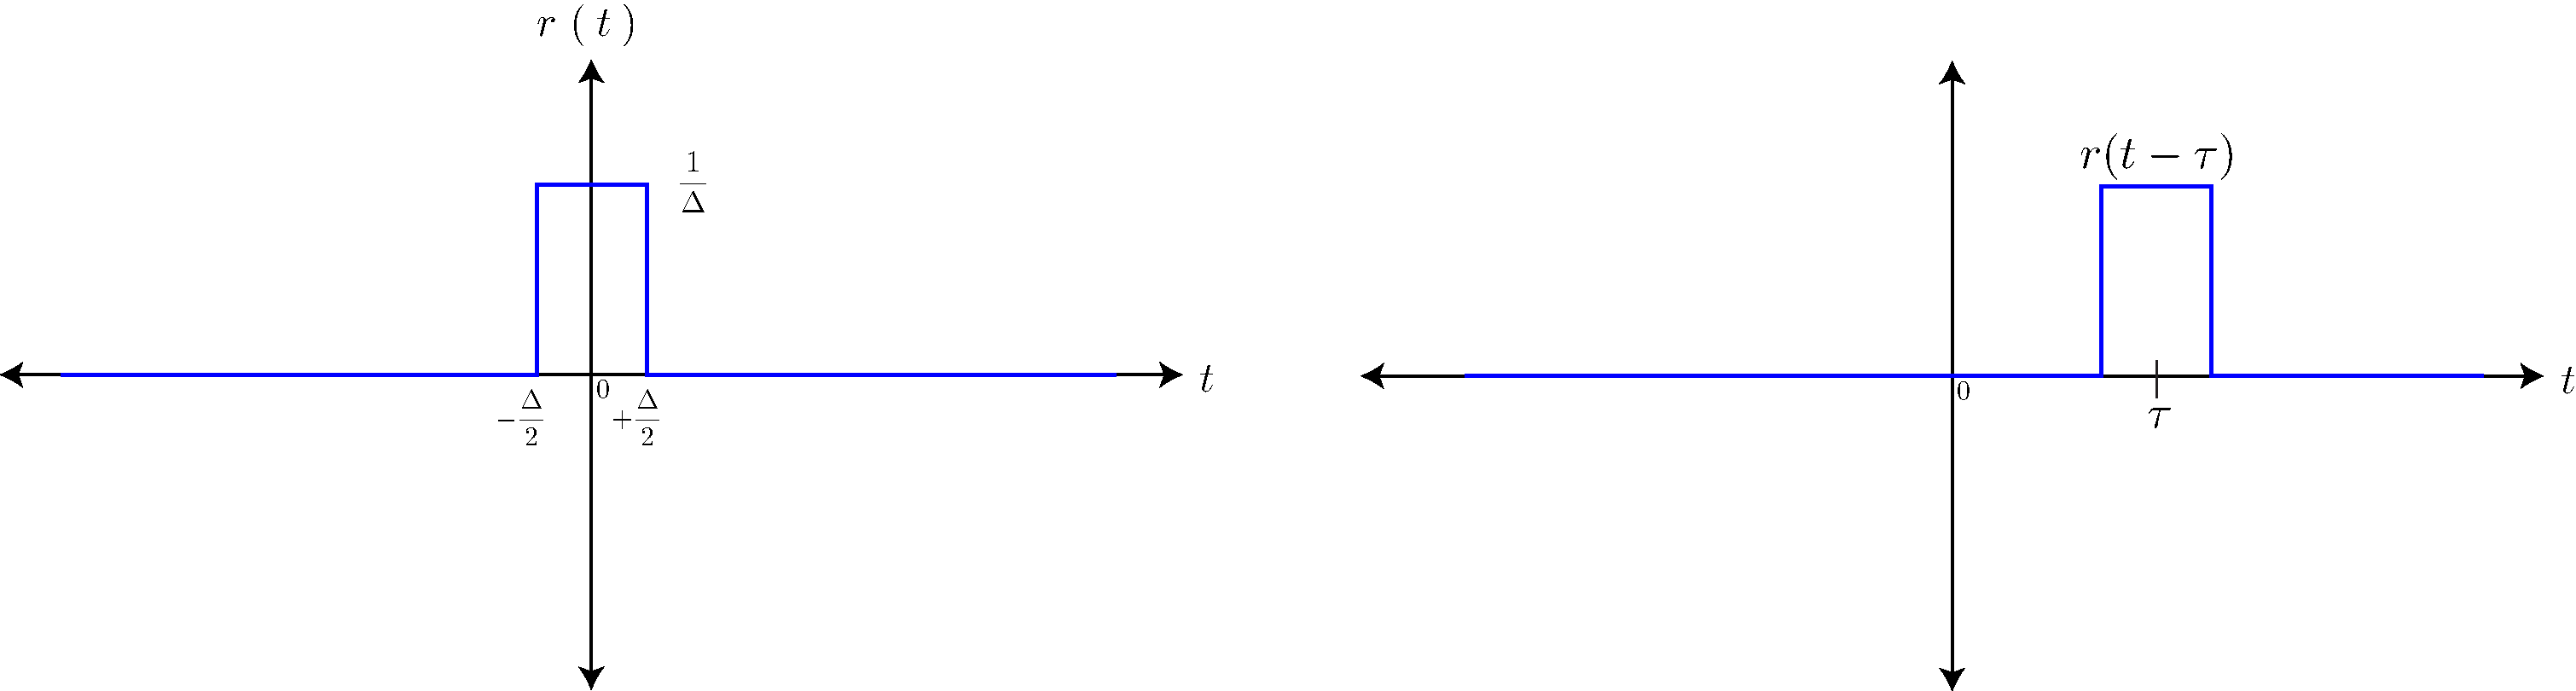
\includegraphics[width=1\columnwidth]{rect_func}
\caption{The unit rectangular function, centered at the origin or shifted by $\tau$. }
\label{fig:fun_rect}
\end{figure}
%%%%%%%%%%%%%%%%%%%%%%%%%%%%%%%%%%%%%%%%%%%%
A very convenient function, the \textbf{unit rectangular function}\index{Unit rectangular function}, shown in \emph{Fig.~\ref{fig:fun_rect}}, is defined as follows.  Consider a rectangular function with unit area:
    \begin{equation}
        r(t) = \left\{ 
        \begin{array}{cc} 
        \frac{1}{\Delta} & -\Delta/2 < t < \Delta/2 \\ 
        0  & \mathrm{otherwise} 
        \end{array} \right.
    \end{equation}
 By definition, we have a unit area function
    \begin{equation}
        \int_{-\infty}^{\infty} r(t) dt = 1
    \end{equation}
%%%%%%%%%%%%%%%%%%%%%%%%%%%%%%%%%%%%%%%%%%%%
%              SUB-SUBSECTION              %
%%%%%%%%%%%%%%%%%%%%%%%%%%%%%%%%%%%%%%%%%%%%
\subsubsection{Function Approximation}
As shown in \emph{Fig. ~\ref{fig:func_rect}}, we can approximate any function as a sum of rectangular shifted functions
    \begin{equation}
        x(t) \approx \sum_i x(i\tau) r(t - i\tau) \Delta
    \end{equation}
 As the rectangles become smaller and smaller, the representation becomes more accurate
 The key question is what happens as we take the limit of a very small time step $\Delta$?
%%%%%%%%%%%%%%%%%%%%%%%%%%%%%%%%%%%%%%%%%%%%
%                 FIGURE                   %
%%%%%%%%%%%%%%%%%%%%%%%%%%%%%%%%%%%%%%%%%%%%
\begin{figure}[tb]
\centering
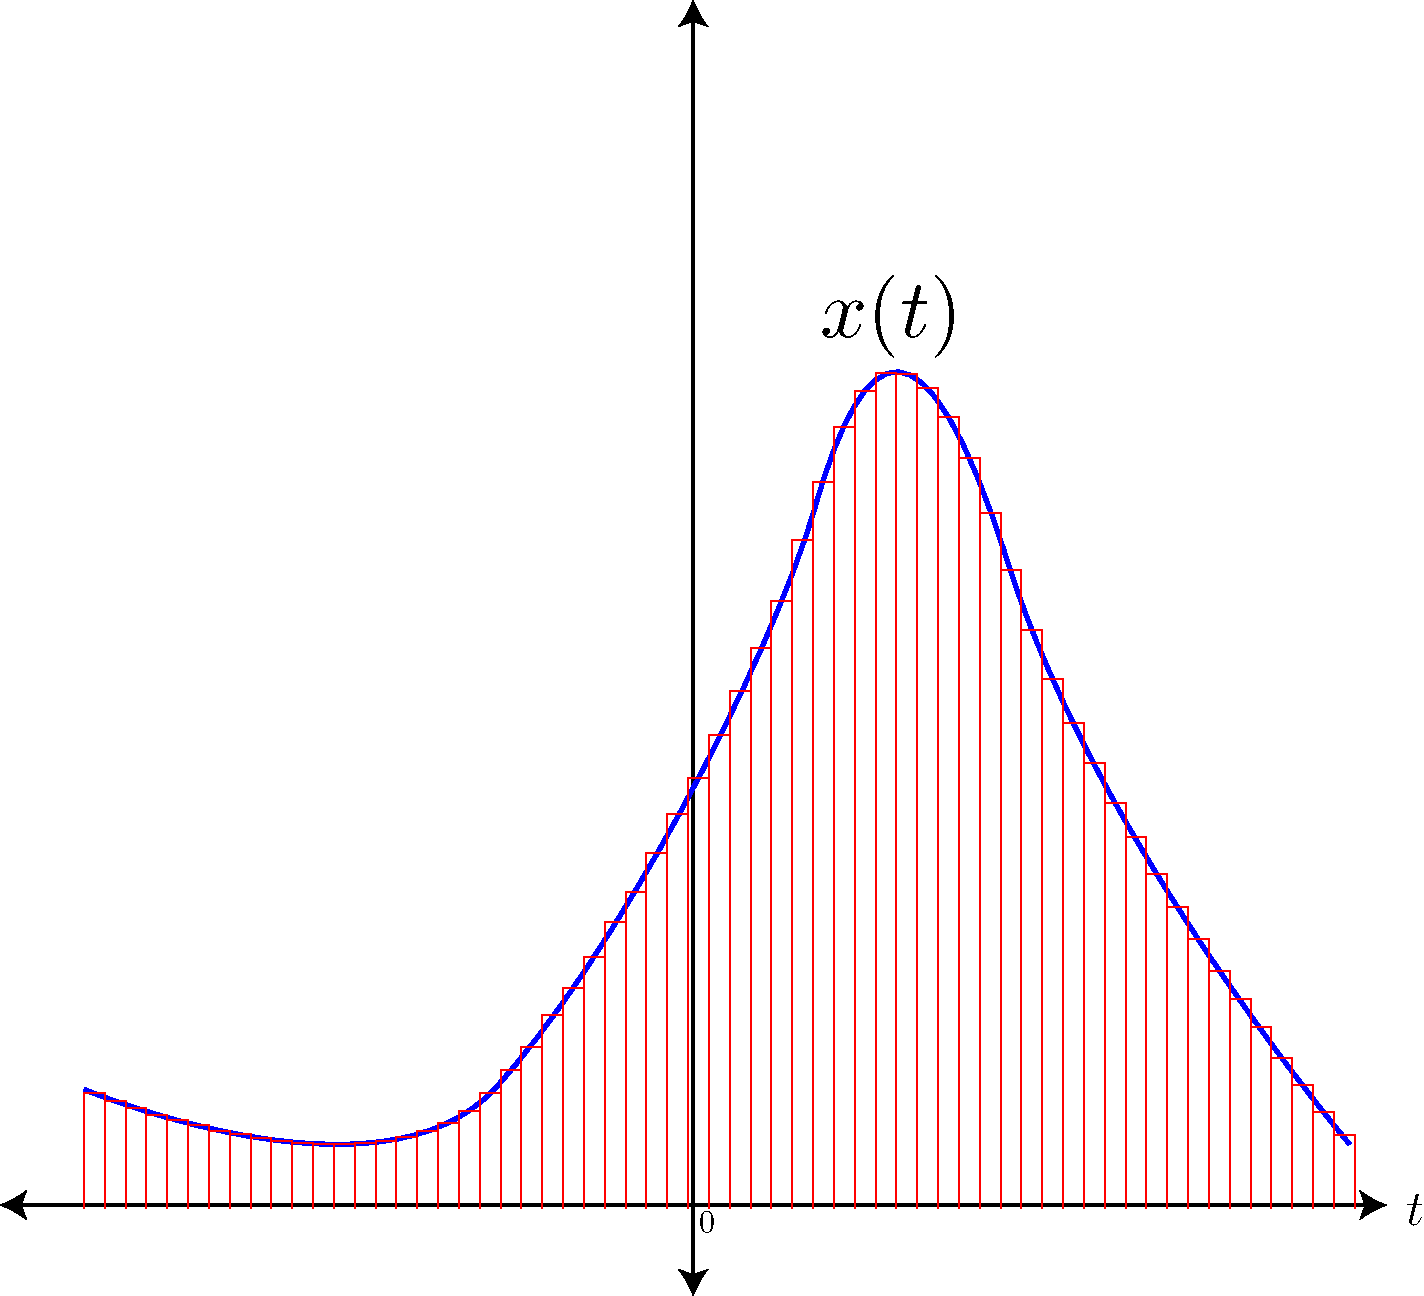
\includegraphics[width=.55\columnwidth]{func_rect}
\caption{Representation of a general function by a sum of shifted rectangular functions. }
\label{fig:func_rect}
\end{figure}
%%%%%%%%%%%%%%%%%%%%%%%%%%%%%%%%%%%%%%%%%%%%
%              SUB-SUBSECTION              %
%%%%%%%%%%%%%%%%%%%%%%%%%%%%%%%%%%%%%%%%%%%%
\subsubsection{The Delta Function $\delta(t)$ -- A Strange Beast}
%%%%%%%%%%%%%%%%%%%%%%%%%%%%%%%%%%%%%%%%%%%%
%                 FIGURE                   %
%%%%%%%%%%%%%%%%%%%%%%%%%%%%%%%%%%%%%%%%%%%%
\begin{figure}[tb]
\centering
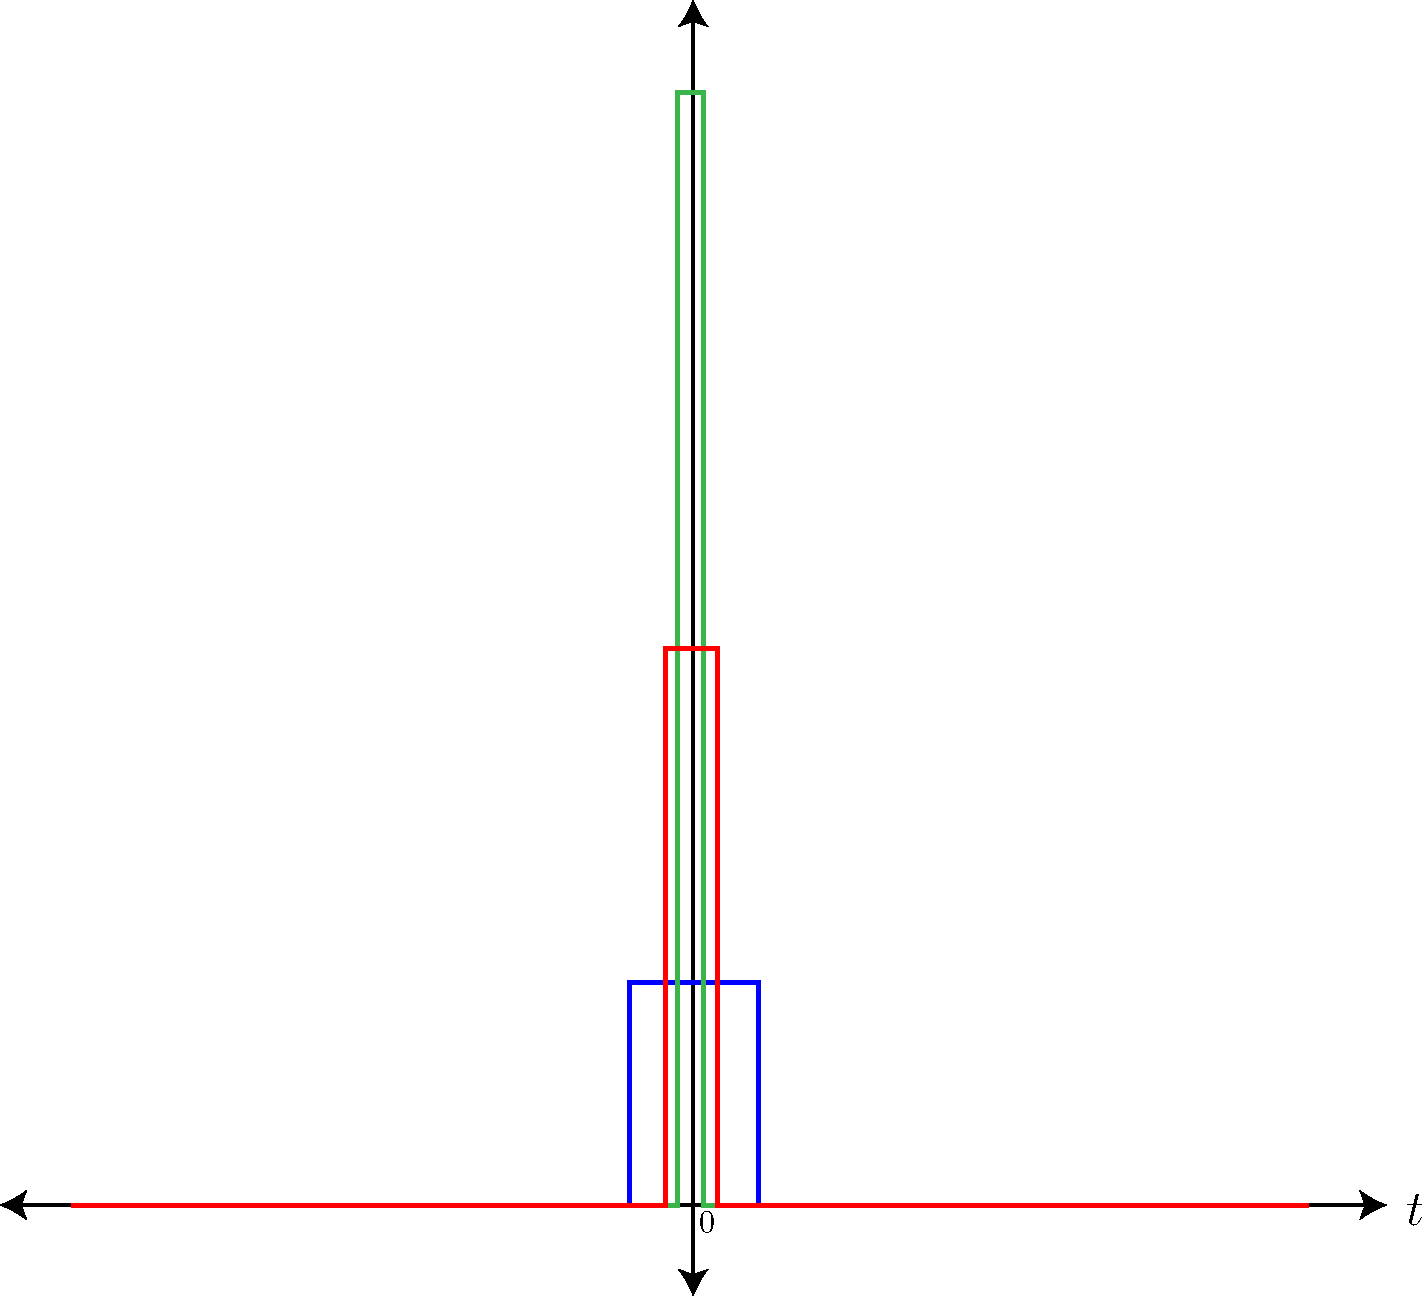
\includegraphics[width=.5\columnwidth]{rect_func_delta}
\caption{The "Delta Function" can be obtained through a limiting process by making the interval of the rectangular function shorter and shorter. }
\label{fig:rect_func_delta}
\end{figure}
%%%%%%%%%%%%%%%%%%%%%%%%%%%%%%%%%%%%%%%%%%%%
Now imagine taking the limit as $\Delta\rightarrow 0$
    \begin{equation}
        \lim_{\Delta\rightarrow0}{r\left(t\right)=\delta(t)}
    \end{equation}
What do we get?  Is this thing even a function?  A pictorial representation of the limiting process is shown in \emph{Fig.~\ref{fig:rect_func_delta}}.  We see that the function becomes more and more narrow and taller and taller.
%%%%%%%%%%%%%%%%%%%%%%%%%%%%%%%%%%%%%%%%%%%%
 No, it's not an ordinary function.\footnote{Mathematicians have made sense of it.  Now it's known as a distribution or generalized function.}  The \textbf{delta function}\index{Dirac Delta Function} was originally introduced by Oliver Heaviside $\sim$1900, Dirac co-invented it and gets credit as it's known as the ``Dirac Delta Function".\footnote{Heaviside was derided by the mathematicians of the day for his methods.  He often got the right answer without being mathematically rigorous, but that's because he was way ahead of everyone in his techniques, and it took a while for the mathematical world to catch up.}
%%%%%%%%%%%%%%%%%%%%%%%%%%%%%%%%%%%%%%%%%%%%
%              SUB-SUBSECTION              %
%%%%%%%%%%%%%%%%%%%%%%%%%%%%%%%%%%%%%%%%%%%%
\subsubsection{Dirac Delta Sifting Property}
%%%%%%%%%%%%%%%%%%%%%%%%%%%%%%%%%%%%%%%%%%%%
%                 FIGURE                   %
%%%%%%%%%%%%%%%%%%%%%%%%%%%%%%%%%%%%%%%%%%%%
\begin{figure}[tb]
\centering
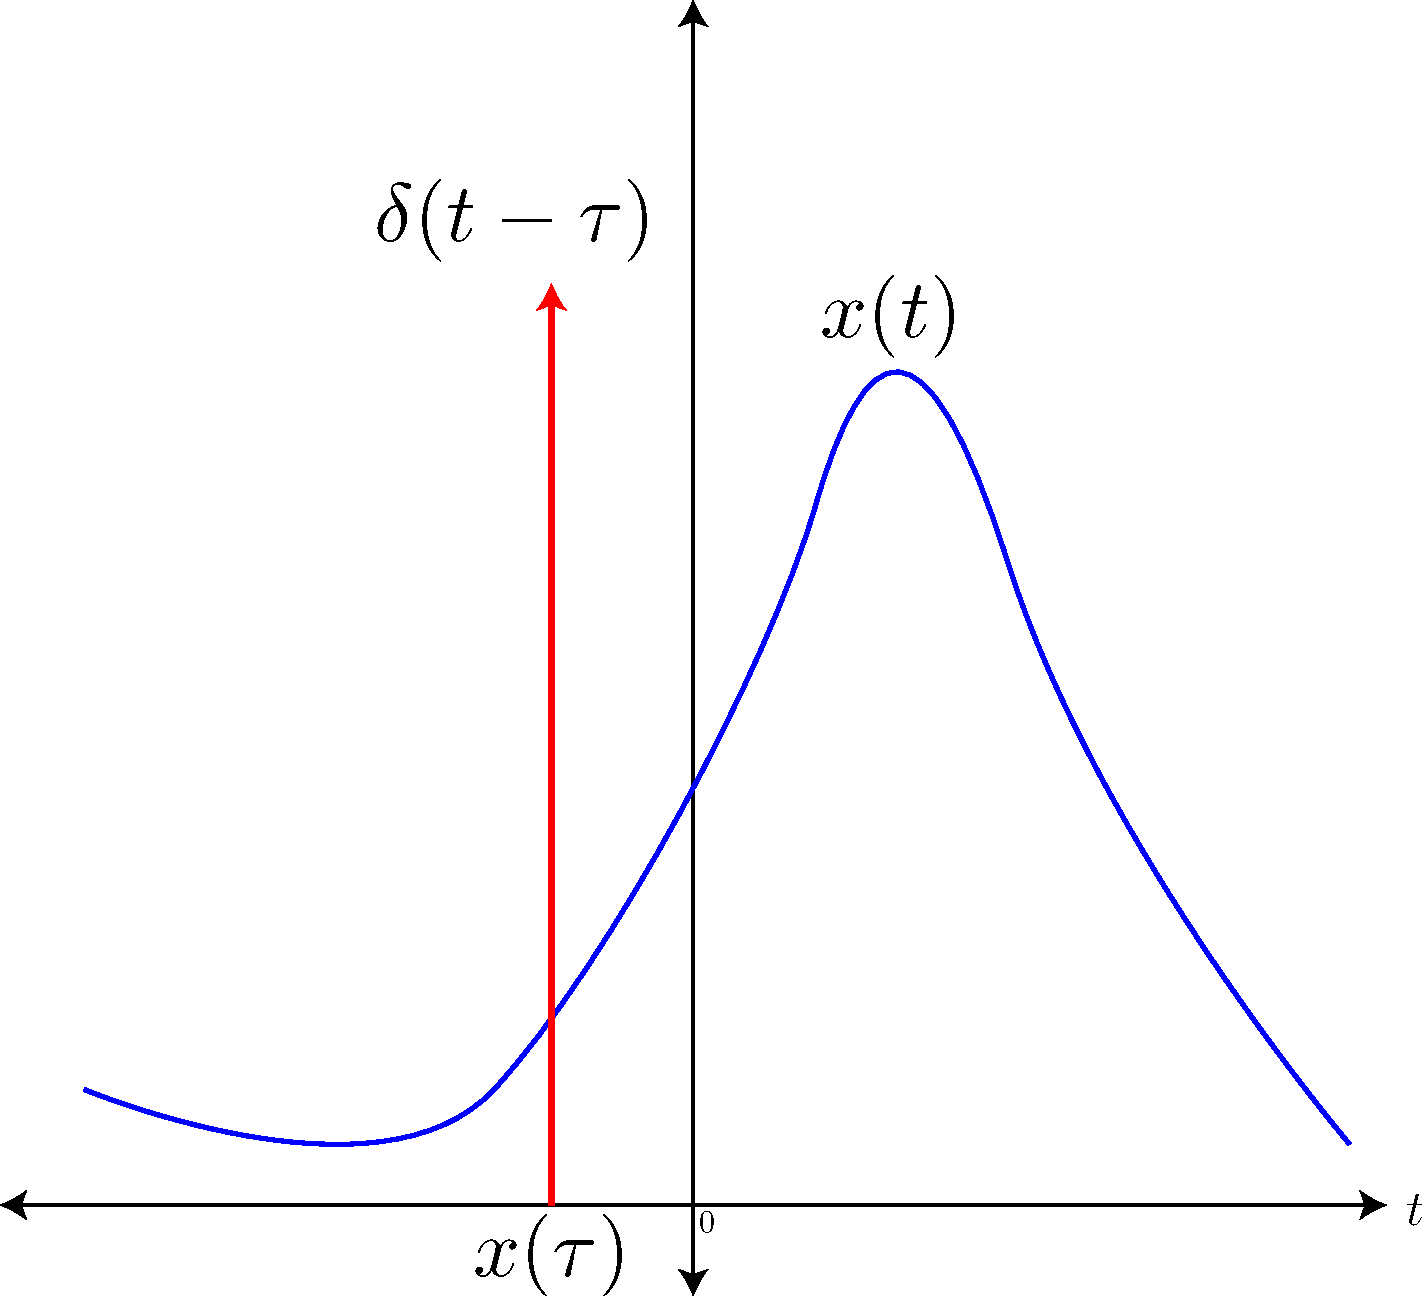
\includegraphics[width=.5\columnwidth]{delta_sift}
\caption{The \textbf{"sifting" property}\index{Dirac Delta Function!sifting property} of the Delta function yields the function value at any point. }
\label{fig:delta_sift}
\end{figure}
%%%%%%%%%%%%%%%%%%%%%%%%%%%%%%%%%%%%%%%%%%%%
As shown in \emph{Fig.~\ref{fig:delta_sift}}, one interesting thing about the Delta function is that it can be used to basically pick out a certain value of a function (because it's zero except at one location):
    \begin{equation}
        x\left(\tau\right)=\int\delta\left(t-\tau\right)x\left(t\right)dt
    \end{equation}
This is not obvious unless you take the limit and then it becomes clear that the integral converges to the value of the function.  So the Dirac Delta function is better defined in terms of this property, and many functions satisfy this function and can be used to define the Delta function.

Recall that we started by using the rectangular function to approximate any arbitrary function.  As we take the limit, we are reconstructing our function point-by-point using weighted sums of Delta functions.  To see this, simply start with the approximated  function as before
    \begin{equation}
        x(t) \approx \sum_i x(i\tau) r(t - i\tau) \Delta
    \end{equation}
As we take the limit, we expect that our approximation becomes more exact and we have the following integral:
    \begin{equation}
        x\left(t\right)=\int x\left(\tau\right)\delta\left(t-\tau\right)d\tau
    \end{equation}
In some ways this is not really a deep result in the sense of  saying that a function is a continuous stream of real numbers, and any particular value can be "sifted" out by multiplying by a delta and integrating around the delta.  If you think of the function as a vector, the delta function is like the vector $e_n = [0 \cdots 0\, 1\, 0 \cdots 0 ]^T$ with the $1$ in the n'th position. 
%%%%%%%%%%%%%%%%%%%%%%%%%%%%%%%%%%%%%%%%%%%%%%%%%%%%%%%%%%%%%%%%%%%%%%%%%%%%%%%%%%%%%%%%
%%%%%%%%%%%%%%%%%%%%%%%%%%%%%%%%%%%%%%%%%%%%%%%%%%%%%%%%%%%%%%%%%%%%%%%%%%%%%%%%%%%%%%%%
%                                   SECTION 1.8                                        %
%%%%%%%%%%%%%%%%%%%%%%%%%%%%%%%%%%%%%%%%%%%%%%%%%%%%%%%%%%%%%%%%%%%%%%%%%%%%%%%%%%%%%%%%
%%%%%%%%%%%%%%%%%%%%%%%%%%%%%%%%%%%%%%%%%%%%%%%%%%%%%%%%%%%%%%%%%%%%%%%%%%%%%%%%%%%%%%%%
\section{Back to Time Domain:  Impulse Response}
Up to now we studied the sinusoidal steady-state response using the complex exponential.  But we are now armed with the right tools to tackle the \textbf{general response}\index{Linear system!general response} of a linear system to an arbitrary input in time.  Using the fundamental properties of linearity and superposition, we have
    \begin{equation}
        y\left(t\right)=\ \mathbf{L}\left[x\left(t\right)\right]=\mathbf{L}\left[\int\delta\left(t-\tau\right)x\left(\tau\right)d\tau\right]
    \end{equation}
    \begin{equation}
        y\left(t\right)=\ \mathbf{L}\left[x\left(t\right)\right]=\int \mathbf{L}\left[\delta\left(t-\tau\right)x\left(\tau\right)\right]d\tau= \int x\left(\tau\right)\mathbf{L}\left[\delta\left(t-\tau\right)\right]d\tau
    \end{equation}
Let's define the impulse function as the response of a linear system to a Delta function applied at time $\tau$
    \begin{equation}
        h(t,\tau) \equiv  \mathbf{L}[\delta(t-\tau)]
    \end{equation}
Notice that in a time-invariant system, it should not matter when we apply the Delta function, as long as we shift the output.  So if $h(t)$ is the response to a Delta function at time 0, $h(t-\tau)$ is the response to an input applied at time $\tau$.  So in summary, for a linear time-invariant system (LTI), we only need to characterize the system response to a Delta function once and for all to find
    \begin{equation}
        h(t) \equiv  \mathbf{L}[\delta(t)]
    \end{equation}
This means that $h(t)$ contains all the information about the linear system. If we call the Dirac Delta function an "impulse", then for obvious reasons, we call $h(t)$ the \textbf{``impulse response function"}\index{Impulse response function}. 
%%%%%%%%%%%%%%%%%%%%%%%%%%%%%%%%%%%%%%%%%%%%
%             SUBSECTION 1.8.1             %
%%%%%%%%%%%%%%%%%%%%%%%%%%%%%%%%%%%%%%%%%%%%
\subsection{Convolution Operation}
We have demonstrated that any linear system input/output response can be represented by the following integral\index{Convolutions!integral}:
    \begin{equation}
        y(t) = \int_{-\infty}^{\infty} h(t-\tau) x(\tau) d\tau 
    \end{equation}
Think of this as the sum of the input weighted by the impulse response function.  The operation is known as the convolution operation and symbolically defined by the operator "$*$":  
    \begin{equation}
        y(t) = h(t) * x(t)
    \end{equation}
The symbol $*$ is the \textbf{convolution operator}\index{Convolutions!operator}. You can also change variables $x = t - \tau$ and write it as:
    \begin{equation}
        y(t) = \int_{\infty}^{-\infty} h(x) x(t-x) (-dx) = \int_{-\infty}^{\infty} h(x) x(t-x) dx 
    \end{equation}
In this equation, $x$ is just a dummy variable.  We can substitute $\tau$ to make the equation look the same as before (recall from calculus that  $\int_b^a x = -\int_a^b x$):
    \begin{equation}
        y(t) =  \int_{-\infty}^{\infty} x(t-\tau) h(\tau) d\tau
    \end{equation}
%%%%%%%%%%%%%%%%%%%%%%%%%%%%%%%%%%%%%%%%%%%%
%              SUB-SUBSECTION              %
%%%%%%%%%%%%%%%%%%%%%%%%%%%%%%%%%%%%%%%%%%%%
\subsubsection{Convolution Visualization}
%%%%%%%%%%%%%%%%%%%%%%%%%%%%%%%%%%%%%%%%%%%%
%                 FIGURE                   %
%%%%%%%%%%%%%%%%%%%%%%%%%%%%%%%%%%%%%%%%%%%%
\begin{figure}[tb]
\centering
\includegraphics[width=.95\columnwidth]{conv_picture.png} 
\caption{The convolution operation visualized.  See Wikipedia for full details and an animation.}
\label{fig:conv_visual}
\end{figure}
%%%%%%%%%%%%%%%%%%%%%%%%%%%%%%%%%%%%%%%%%%%%
It's useful to visualize the convolution operation.  Note that the convolution operation takes in two functions and produces a new function.  The operation is described nicely on Wikipedia\footnote{\url{https://en.wikipedia.org/wiki/Convolution}} reproduced here in \emph{Fig.~\ref{fig:conv_visual}}.  As described in the figure, we first express each function in terms of the dummy variable (of integration) $\tau$.  Next, we reflect one of the functions about the time axis.  For example, $h(\tau)$ becomes $h(-\tau)$.  The physical explanation for this will be described shortly.  Next we compute a sliding weighted-sum of the function $x(\tau)$ with $h(t-\tau)$.  Only points where the two functions intersect contribute significantly to the waveform.  
%%%%%%%%%%%%%%%%%%%%%%%%%%%%%%%%%%%%%%%%%%%%
%              SUB-SUBSECTION              %
%%%%%%%%%%%%%%%%%%%%%%%%%%%%%%%%%%%%%%%%%%%%
\subsubsection{Memory}
%%%%%%%%%%%%%%%%%%%%%%%%%%%%%%%%%%%%%%%%%%%%
%                 FIGURE                   %
%%%%%%%%%%%%%%%%%%%%%%%%%%%%%%%%%%%%%%%%%%%%
\begin{figure}[tb]
\begin{tabular}{cc}
\includegraphics[width=.4\columnwidth]{impulse1_long.pdf} &
\includegraphics[width=.4\columnwidth]{impulse2_short.pdf} \\
\end{tabular}
\caption{Two hypothetical impulse response functions are shown.  One is long and oscillates, the second is short and delays exponentially.}
\label{fig:memory}
\end{figure}
%%%%%%%%%%%%%%%%%%%%%%%%%%%%%%%%%%%%%%%%%%%%
For example, if $h(t)$ is mostly zero except over a small interval, 
%%%%%%%%%%%%%%%%%%%%%%%%%%%%%%%%%%%%%%%%%%%%
The fact that the impulse response function has time duration is an indication that the system has memory.  The current output depends not only on the current input, but also past values of the input.  The longer the duration of the impulse response function, the more ``memory" the system has.  Capacitors and inductors store energy and act as memory in circuits.  They store energy in the magnetic and electric fields, and resonance can occur because these forms of energy can be exchanged.  The impulse response function for a system with no memory is just another delta function!  Two examples are shown in \emph{Fig.~\ref{fig:memory}} to illustrate a system with a longer vacillating impulse response versus a system that has a short and exponentially decaying impulse response.  

This should help you understand why we needed to flip the impulse response in the convolution operation (or equivalently the input function).  Notice first that the impulse function is necessarily zero until time zero. This is because the system is causal and there can be no output if there's no input.  Next, notice that by flipping the impulse response and taking a sliding weighted sum with the input, we're including the contribution of past inputs on the current input.  If the impulse response is short and decaying exponentially, then only a small amount of past inputs influence the current input.  On the other hand, if the impulse response is longer, then the system remembers the history of the input for a longer duration and we must include those terms to figure out the current output.
%%%%%%%%%%%%%%%%%%%%%%%%%%%%%%%%%%%%%%%%%%%%
%              SUB-SUBSECTION              %
%%%%%%%%%%%%%%%%%%%%%%%%%%%%%%%%%%%%%%%%%%%%
\subsubsection{The Delta Function ``Hammer":  Mechanical Analogy}
%%%%%%%%%%%%%%%%%%%%%%%%%%%%%%%%%%%%%%%%%%%%
%                 FIGURE                   %
%%%%%%%%%%%%%%%%%%%%%%%%%%%%%%%%%%%%%%%%%%%%
\begin{figure}[tb]
\centering
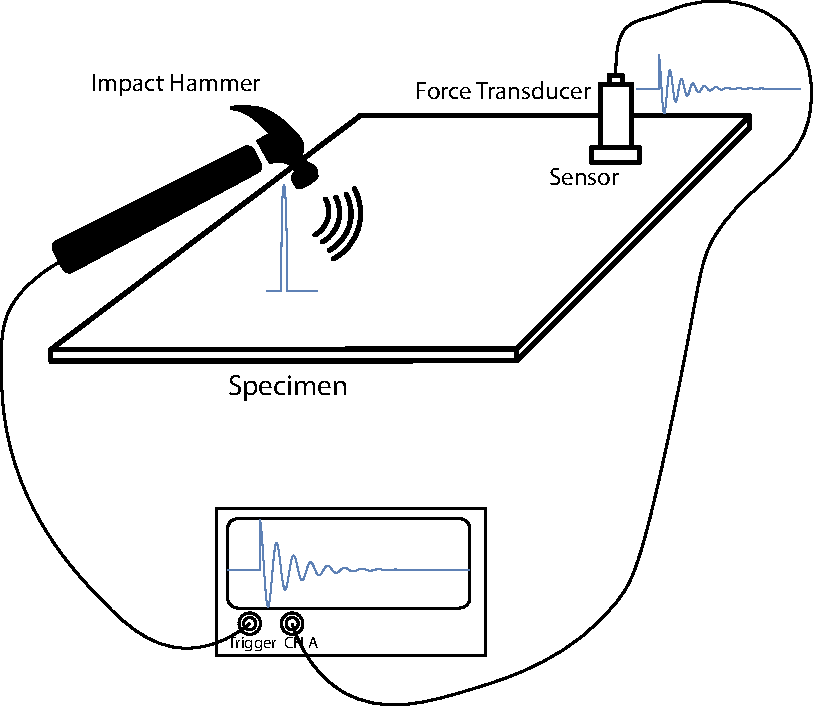
\includegraphics[width=.5\columnwidth]{hammer_resonance}
\caption{A measurement setup to record the impulse response of a mechanical system. }
\label{fig:hammer_setup}
\end{figure}
%%%%%%%%%%%%%%%%%%%%%%%%%%%%%%%%%%%%%%%%%%%%
Another way to look at a delta function is to think of it like hitting your system with a hammer (see \emph{Fig.~\ref{fig:hammer_setup}}).  It is an impulsive input that excites the system.  After such an excitation, the system will ``vibrate" in its natural modes and these vibrations will eventually die out.  The time that the vibrations last is related to the depth of the system's memory.  The vibrations are related to the fact that the system can store kinetic and potential energy and these modes complement each other.  Loss in the system causes this stored energy to eventually dissipate.  In fact, one way to measure the impulse response is exactly with the setup shown.  The hammer is implemented an electromechanical solenoid, and the actuation signal is fed to the trigger of the oscilloscope (or other recording device).  The vibrations are picked up by a force transducer and carefully recorded, yielding the impulse response.     
%%%%%%%%%%%%%%%%%%%%%%%%%%%%%%%%%%%%%%%%%%%%%%%%%%%%%%%%%%%%%%%%%%%%%%%%%%%%%%%%%%%%%%%%
%%%%%%%%%%%%%%%%%%%%%%%%%%%%%%%%%%%%%%%%%%%%%%%%%%%%%%%%%%%%%%%%%%%%%%%%%%%%%%%%%%%%%%%%
%                                   SECTION 1.9                                        %
%%%%%%%%%%%%%%%%%%%%%%%%%%%%%%%%%%%%%%%%%%%%%%%%%%%%%%%%%%%%%%%%%%%%%%%%%%%%%%%%%%%%%%%%
%%%%%%%%%%%%%%%%%%%%%%%%%%%%%%%%%%%%%%%%%%%%%%%%%%%%%%%%%%%%%%%%%%%%%%%%%%%%%%%%%%%%%%%%
\section{Step and Pulse Response}
%%%%%%%%%%%%%%%%%%%%%%%%%%%%%%%%%%%%%%%%%%%%
%                 FIGURE                   %
%%%%%%%%%%%%%%%%%%%%%%%%%%%%%%%%%%%%%%%%%%%%
\begin{figure}[tb]
\centering
\includegraphics[width=.6\columnwidth]{impulse_resp}
\caption{The impulse response for the low-pass filtered analyzed earlier in the frequency domain. }
\label{fig:impulse_resp}
\end{figure}
%%%%%%%%%%%%%%%%%%%%%%%%%%%%%%%%%%%%%%%%%%%%
Consider a system with an impulse response shown in \emph{Fig.~\ref{fig:impulse_resp}}.  This is in fact the impulse response function for a low-pass filter:\footnote{See tables~\ref{fig:laplace_table} and~\ref{fig:laplace_xform} of transforms later in this lecture.}
    \begin{equation}
        h(t) = u(t) \frac{1}{\tau} e^{-t/\tau}
    \end{equation}
Notice that the system has a time constant $\tau = RC$ that corresponds to the amount of time the system responds to an impulse input ($\tau = 1/3$).  Here $u(t)$ is the step function (zero until time zero, and then unity thereafter).  As discussed earlier, the impulse response is necessarily zero until time zero, and the $u(t)$ enforces this condition.  If you now imagine an arbitrary input, each time point is a weighted sum of the current input and past inputs, with an exponentially decaying amplitude for past inputs.  Only the recent $\sim \tau$ inputs really make an impact, and earlier inputs are ``forgotten".  
%%%%%%%%%%%%%%%%%%%%%%%%%%%%%%%%%%%%%%%%%%%%
%                 FIGURE                   %
%%%%%%%%%%%%%%%%%%%%%%%%%%%%%%%%%%%%%%%%%%%%
\begin{figure}[tb]
\centering
\includegraphics[width=.5\columnwidth]{step_resp}
\caption{The step response of a low-pass filter. }
\label{fig:step_resp}
\end{figure}
%%%%%%%%%%%%%%%%%%%%%%%%%%%%%%%%%%%%%%%%%%%%
%             SUBSECTION 1.9.1             %
%%%%%%%%%%%%%%%%%%%%%%%%%%%%%%%%%%%%%%%%%%%%
\subsection{Step Response}
A very interesting input is the \textbf{"step input"}\index{Step input}\index{Step response}, or application of $u(t)$ to our system.  From what we know, we can calculate the response to a step by using a convolution:
    \begin{equation}
        y(t) = h(t) * u(t) = \left( 1 - e^{-3 t} \right) u(t) 
    \end{equation}
The response is plotted in \emph{Fig.~\ref{fig:step_resp}}. The step has a very sharp transition at the input, but at the output it's smoothed out because each output point is an average of the current input and past inputs.  Since at the moment of the transition, all past inputs are zero, the output cannot track the input instantaneously.
\newpage
%%%%%%%%%%%%%%%%%%%%%%%%%%%%%%%%%%%%%%%%%%%%
%             SUBSECTION 1.9.2             %
%%%%%%%%%%%%%%%%%%%%%%%%%%%%%%%%%%%%%%%%%%%%
\subsection{Sinusoidal Response}
%%%%%%%%%%%%%%%%%%%%%%%%%%%%%%%%%%%%%%%%%%%%
%                 FIGURE                   %
%%%%%%%%%%%%%%%%%%%%%%%%%%%%%%%%%%%%%%%%%%%%
\begin{figure}[tb]
\centering
\begin{tabular}{cc}
\includegraphics[width=.45\columnwidth]{slow_sine.pdf} &
\includegraphics[width=.45\columnwidth]{fast_sine.pdf} \\
\end{tabular}
\caption{The response of a linear system to a "slow" and "fast" sinusoid.  Slow means the period of oscillation is smaller than the filter characteristic time constant $\tau$.  Fast means the opposite.}
\label{fig:fast_slow_resp}
\end{figure}
%%%%%%%%%%%%%%%%%%%%%%%%%%%%%%%%%%%%%%%%%%%%
As shown in \emph{Fig.~\ref{fig:fast_slow_resp}}, if the input changes slower than the time scale of $\tau$, or if the frequency of the input is lower than roughly $1/\tau$, then the output is a smoothed version of the input (each time point is blurred by the width of the impulse response).  Fast transitions are smoothed out and don't appear at the output.   If the input changes very quickly, several cycles of the input are averaged out and produce only a small output.  This is how the filter works as high frequency signals are attenuated by the low-pass filter.  If the oscillation frequency is very slow with respect to $\tau$, the impulse response "looks like" a delta function with no memory and just passes the current input to the output.
%%%%%%%%%%%%%%%%%%%%%%%%%%%%%%%%%%%%%%%%%%%%
%             SUBSECTION 1.9.2             %
%%%%%%%%%%%%%%%%%%%%%%%%%%%%%%%%%%%%%%%%%%%%
\subsection{Pulse Response}
%%%%%%%%%%%%%%%%%%%%%%%%%%%%%%%%%%%%%%%%%%%%
%                 FIGURE                   %
%%%%%%%%%%%%%%%%%%%%%%%%%%%%%%%%%%%%%%%%%%%%
\begin{figure}[tb]
\centering
\begin{tabular}{cc}
\includegraphics[width=.4\columnwidth]{long_pulse.pdf} &
\includegraphics[width=.4\columnwidth]{fast_pulse.pdf} \\
\end{tabular}
\caption{The \textbf{pulse response}\index{Pulse response} of a low-pass filter.  Note that the shorter pulse has been expanded for clarity (see the time scale). }
\label{fig:pulse_resp}
\end{figure}
%%%%%%%%%%%%%%%%%%%%%%%%%%%%%%%%%%%%%%%%%%%%
Now let's see what happens to a pulse.  By superposition, this is just two unit-step responses, so we can easily reconstruct the response as shown in \emph{Fig.~\ref{fig:pulse_resp}}.  If the pulse is wide, then the output has enough time to settle and the output pulse is a faithful representation of the input.  If the pulse width is shorter than the time-constant of the filter, there is insufficient time for the output to settle, and the pulse is distorted.  In high speed communication systems, we need to ensure the system has enough \textbf{bandwidth}\index{Bandwidth} to allow the highest frequency pulses to get through.  
%%%%%%%%%%%%%%%%%%%%%%%%%%%%%%%%%%%%%%%%%%%%%%%%%%%%%%%%%%%%%%%%%%%%%%%%%%%%%%%%%%%%%%%%
%%%%%%%%%%%%%%%%%%%%%%%%%%%%%%%%%%%%%%%%%%%%%%%%%%%%%%%%%%%%%%%%%%%%%%%%%%%%%%%%%%%%%%%%
%                                   SECTION 1.10                                       %
%%%%%%%%%%%%%%%%%%%%%%%%%%%%%%%%%%%%%%%%%%%%%%%%%%%%%%%%%%%%%%%%%%%%%%%%%%%%%%%%%%%%%%%%
%%%%%%%%%%%%%%%%%%%%%%%%%%%%%%%%%%%%%%%%%%%%%%%%%%%%%%%%%%%%%%%%%%%%%%%%%%%%%%%%%%%%%%%%
\section{Frequency Domain Characterization of Linear Systems}
We started this chapter by discussion of the steady-state sinusoidal response of a linear system.  We found that we can use complex exponential inputs to quickly and efficiently calculate the output, and by sweeping the frequency, we obtain the \textbf{spectral response}\index{Spectral response} of the system $H(s)$ (the complex eigenvalues) that completely characterizes the system.   Next we find that in the time domain, the impulse response is a way to "probe" a linear system to determine its behavior.  In other words both $H(s)$ and $h(t)$ are a very special responses that characterizes the system.  One comes from the complex exponential input $e^{st}$ and the other from the the application of a delta function.  How are these functions $H(s)$ and $h(t)$ related?
%%%%%%%%%%%%%%%%%%%%%%%%%%%%%%%%%%%%%%%%%%%%
%             SUBSECTION 1.10.1            %
%%%%%%%%%%%%%%%%%%%%%%%%%%%%%%%%%%%%%%%%%%%%
\subsection{Relation to Complex Exponential}
Recall that we found that the complex exponential\index{Complex exponential} is an eigenfunction\index{Eigenfunction} for our linear system:
    \begin{equation}
        \mathbf{L} [ e^{st} ] = H(s) e^{st}
    \end{equation}
But that means that we can apply the convolution integral\index{Convolutions!integral} to the input $e^{st}$ and equate the two outputs:
    \begin{equation}
        \mathbf{L} [ e^{st} ] = H(s) e^{st}  = \int_{-\infty}^{\infty} h(t-\tau) e^{s\tau} d\tau
    \end{equation}
A simple manipulation shows that:
    \begin{align*}
        H(s) &= \int h(t-\tau) e^{s\tau} e^{-st} d\tau\\
        &= \int h(t-\tau) e^{-s(t- \tau)} d\tau\\
        &= \int_{\infty}^{-\infty} h(x) e^{-sx} (-dx) &\text{\emph{Let $x = t - \tau$}}
    \end{align*}
Thus, we have:
    \begin{equation}
        H(s) = \int_{-\infty}^{\infty} h(x) e^{-sx} dx
    \end{equation}
This equation shows us that $H(s)$ and $h(t)$ are indeed related in a very special way.
%%%%%%%%%%%%%%%%%%%%%%%%%%%%%%%%%%%%%%%%%%%%
%              SUB-SUBSECTION              %
%%%%%%%%%%%%%%%%%%%%%%%%%%%%%%%%%%%%%%%%%%%%
\subsubsection{Laplace Transform}
 We derived a very important relation between the transfer function and the impulse response which is known as the \textbf{Laplace Transform}\index{Laplace transform} $\mathcal{L}$:
    \begin{equation}
        H(s) = \int_{-\infty}^{\infty} h(t) e^{-st} dt = \mathcal{L} \left\{ h(t) \right\}
    \end{equation}
This can be interpreted as transforming a \textbf{time-domain}\index{Time-domain} function to the \textbf{``s-domain"}\index{S-domain}, which is the general complex \textbf{frequency-domain}\index{Frequency-domain}.  In this book we will not use Laplace Transforms explicitly, instead we will mostly use the transfer function in the frequency domain:  $H(j\omega)$, which is nothing but evaluating the transfer function $H(s)$ for $s=j\omega$.  
%%%%%%%%%%%%%%%%%%%%%%%%%%%%%%%%%%%%%%%%%%%%
Even though we won't make extensive use of the Laplace Transform, we nevertheless spent some time to highlight these important concepts and relations because they show a deep connection between the frequency domain response $H(j\omega)$ and the time domain response.
%%%%%%%%%%%%%%%%%%%%%%%%%%%%%%%%%%%%%%%%%%%%
%             SUBSECTION 1.10.2            %
%%%%%%%%%%%%%%%%%%%%%%%%%%%%%%%%%%%%%%%%%%%%
\subsection{De-convolving the Convolution}
In fact, one of the most important relations is how convolution in time translates to the frequency domain.  Consider the (complicated) convolution operator and take the results into the Laplace domain:
    \begin{equation}
        Y(s) = \mathcal{L} \left\{ x(t) * h(t) \right\} = \mathcal{L} \left\{  \int h(t-\tau) x(\tau) d\tau \right\} 
    \end{equation}
Use the definition of the Laplace Transform
    \begin{equation}
        Y(s) = \int \left( \int h(t-\tau) x(\tau) d\tau \right) e^{-s t} dt
    \end{equation}
Notice that if we make a simple change of notation and call $y = t-\tau$ the new dummy variable, we have:
    \begin{align*}
        Y(s) &= \int \int h(\underbrace{t-\tau}_{y}) x(\tau) e^{-s t} d\tau dt\\
        &= \int \int h(y) e^{-s(y + \tau)} x(\tau) dy d\tau &\text{\emph{$t = y + \tau$}}
    \end{align*}
Each integral is only a function of one variable, so we can separate them out:
    \begin{equation}
        Y(s) = \left( \int h(y) e^{-sy} dy \right) \left( \int x(\tau) e^{-s \tau} d\tau \right)
    \end{equation}
 Or more simply, the convolution is a (simple) product in the Laplace domain:
    \begin{equation}
        Y(s) = H(s) X(s) 
    \end{equation}
This is a very important result.  Not only is it more efficient to work directly in the \textbf{Laplace domain}\index{Laplace domain} (or frequency domain) when computing the response of a linear system, but it is also much easier to visualize what's going on.  A filter can be visualized very simply in the frequency domain. For an arbitrary input, if we compute it's Laplace (or Fourier, see below) Transform, we can find the output by simply multiplying the two and doing an inverse transform.  In many cases, we don't even need to do the inverse transform, which is not a very simple calculation to carry out.  We simply use the concept of frequency domain to better understand our system.
%%%%%%%%%%%%%%%%%%%%%%%%%%%%%%%%%%%%%%%%%%%%
%              SUB-SUBSECTION              %
%%%%%%%%%%%%%%%%%%%%%%%%%%%%%%%%%%%%%%%%%%%%
\subsubsection{Laplace Transform Properties}
The properties of the Laplace Transform are summarized in \emph{Fig.~\ref{fig:laplace_table}}.   Most are easily derived and are provided here just for reference.  We just proved the most important property related to the convolution.    
%%%%%%%%%%%%%%%%%%%%%%%%%%%%%%%%%%%%%%%%%%%%
%              SUB-SUBSECTION              %
%%%%%%%%%%%%%%%%%%%%%%%%%%%%%%%%%%%%%%%%%%%%
\subsubsection{Laplace Transform Table}
From Wikipedia\footnote{\url{https://en.wikipedia.org/wiki/Laplace_transform}}, the table in \emph{Fig.~\ref{fig:laplace_xform}} shows some common Laplace Transform "pairs", or the s-domain representation for some common functions.  This table is important because in practice we hardly ever evaluate the Laplace Transform integral, especially in the reverse direction.  Instead, the lookup table is used for common functions and special techniques, such as partial fraction expansions, can be used to put a rational function into standard form.  We showed earlier that most linear systems do in fact generate a rational function transfer function.
\newpage
%%%%%%%%%%%%%%%%%%%%%%%%%%%%%%%%%%%%%%%%%%%%
%                 FIGURE                   %
%%%%%%%%%%%%%%%%%%%%%%%%%%%%%%%%%%%%%%%%%%%%
\begin{figure}[tb]
\centering
\includegraphics[width=.85\columnwidth]{laplace_table.png}
\caption{Table of Laplace Transform properties from the Wikipedia site.}
\label{fig:laplace_table}
\end{figure}
%%%%%%%%%%%%%%%%%%%%%%%%%%%%%%%%%%%%%%%%%%%%
%                 FIGURE                   %
%%%%%%%%%%%%%%%%%%%%%%%%%%%%%%%%%%%%%%%%%%%%
\begin{figure}[H]
\centering
\includegraphics[width=.85\columnwidth]{laplace_transform.png}
\caption{Table of Laplace Transform pairs from the Wikipedia site.}
\label{fig:laplace_xform}
\end{figure}
%%%%%%%%%%%%%%%%%%%%%%%%%%%%%%%%%%%%%%%%%%%%
%             SUBSECTION 1.10.3            %
%%%%%%%%%%%%%%%%%%%%%%%%%%%%%%%%%%%%%%%%%%%%
\subsection{Fourier Series and Transform}
In previous courses, you may have learned that you can represent a periodic function in time as a \textbf{Fourier series}\index{Fourier series}
    \begin{equation}
        x(t) = \sum_{n = -\infty}^{\infty} c_n e^{j 2 \pi n f_0 t}
        \label{eq:fourier_series}
    \end{equation}
In this equation $f_0 = 1/T$ is the fundamental frequency of the function of period $T$.  For many practical signals of interest, we can go back and forth between the time or frequency domain, in the sense that the coefficients $c_n$ are a complete representation of the signal (invertable).  The FFT (\textbf{Fast Fourier Transform}\footnote{see Appendix~\ref{app:fft} for a review of the FFT}) is an efficient way to compute the Fourier Series.   We know that the magnitude of the coefficients $c_n$ determine the amount of power concentrated around a certain frequency.  If a function varies gradually in time with a time scale say less than $T$, then coefficients above $n =  f_0 T $ will be smaller in magnitude.

The Fourier Transform is a natural extension of the Fourier Series into the continuous time domain and it works for non-periodic functions (it has a line spectrum for periodic functions)
    \begin{equation}
        X(\omega)  = \mathcal{F} \left\{ x(t) \right\} =  \int_{-\infty}^{\infty} e^{-j \omega t} x(t) dt
    \end{equation}
And the inverse transform is given by
    \begin{equation}
        x(t) =  \mathcal{F}^{-1} \left\{ x(t) \right\} = \int_{-\infty}^{\infty} e^{j \omega t} X(f) df
    \end{equation}
For most signals, this is a well defined transformation allowing us to think of a signal in either the time domain or frequency domain. Notice that the Fourier Transform is related to the Laplace Transform by
    \begin{equation}
        \mathcal{F} \left\{ x(t) \right\}  = \left. X(s) \right|_{s = j\omega}  = X(j\omega)
    \end{equation}
This brings us full circle and shows that the frequency response $H(j\omega)$, the sinusoidal steady-state response, is in fact related to the Laplace Transform of the impulse response of our system.  While $H(s)$ is general, $H(j\omega)$, or the Fourier Transform of the impulse response, it a special case that applies to the periodic steady-state response.  
%%%%%%%%%%%%%%%%%%%%%%%%%%%%%%%%%%%%%%%%%%%%
%             SUBSECTION 1.10.4            %
%%%%%%%%%%%%%%%%%%%%%%%%%%%%%%%%%%%%%%%%%%%%
\subsection{Frequency Domain Interpretation}
If we transform the input function from the time domain to the frequency domain, then we can simply say that every frequency component in the input gets multiplied and phase shifted by the corresponding frequency domain component of the transfer function, as shown in \emph{Fig.~\ref{fig:freq_domain}}.
%%%%%%%%%%%%%%%%%%%%%%%%%%%%%%%%%%%%%%%%%%%%
%                 FIGURE                   %
%%%%%%%%%%%%%%%%%%%%%%%%%%%%%%%%%%%%%%%%%%%%
\begin{figure}[H]
\centering
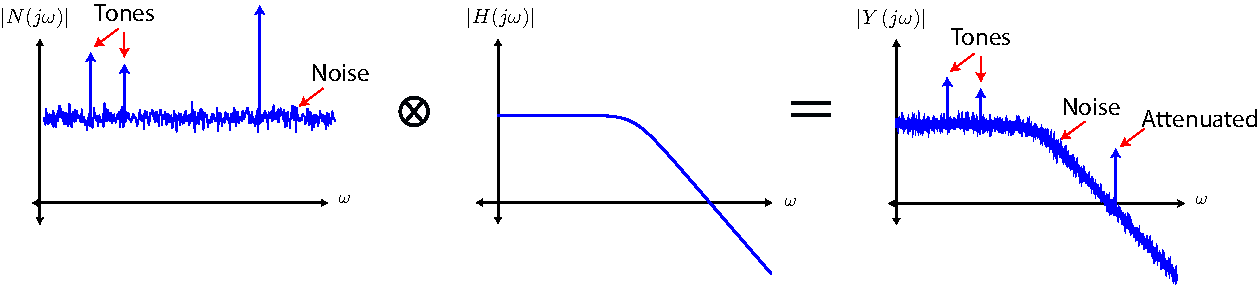
\includegraphics[width=\columnwidth]{sig_noise_freq.pdf}
\caption{The frequency domain representation of a signal plus noise (left).  The signal consists of tones (delta-functions in frequency domain) and noise (flat spectrum).  The signal is low-pass filtered, which is equivalent to multiplication by the frequency domain transfer function shown in the middle, resulting in the filtered signal and reduction in noise (right).}
\label{fig:freq_domain}
\end{figure}
%%%%%%%%%%%%%%%%%%%%%%%%%%%%%%%%%%%%%%%%%%%%
This follows from the properties of convolution in time becoming multiplication in the frequency domain.  Understanding a filter is much, much easier when is it analyzed in the frequency domain.  In this example we see a frequency domain representation of a signal with three tones, shown as Delta functions.  They are delta functions because the input signal consists of pure tones with a very long duration, and so all the energy is concentrated in these two frequency bands.  We also show that the signal is accompanied by "white noise", shown as a flat spectrum signal.  Although we have not proven this yet, it can be shown that noise is a wideband signal and can be modeled as a flat signal in the frequency domain.

If we low-pass filter the signal and noise, we expect that we will reduce the contribution of the noise.  In this example we suppose that the third tone is undesired, so we select the corner frequency of the filter just beyond the second tone, so that we do not attenuate the desired tones.  After filtering,   we would expect that the overall noise of the signal can be reduced without affecting the signals of interest.  This is shown by simply multiplying the frequency domain representation of the signal and noise with the filter response.  We see the noise contribution beyond the corner is reduced dramatically, and the third tone is also attenuated.
%%%%%%%%%%%%%%%%%%%%%%%%%%%%%%%%%%%%%%%%%%%%
%              SUB-SUBSECTION              %
%%%%%%%%%%%%%%%%%%%%%%%%%%%%%%%%%%%%%%%%%%%%
\subsubsection{Audio Example}
In this example, the input signal consists of a pure tone (261.626 Hz) and its third harmonic, which is delayed with respect to the fundamental.  Also, the signal is corrupted by a lot of noise content.  The signals of interest are shown in \emph{Fig.~\ref{fig:tones_time}}.  Now consider the signal + noise with noise power 10$\times$ lower (Signal-Noise Ratio (SNR) = 10 dB), as shown in \emph{Fig.~\ref{fig:sigplusnoise}}.
%%%%%%%%%%%%%%%%%%%%%%%%%%%%%%%%%%%%%%%%%%%%
%                 FIGURE                   %
%%%%%%%%%%%%%%%%%%%%%%%%%%%%%%%%%%%%%%%%%%%%
\begin{figure}[H]
\centering
\begin{tabular}{cc}
\includegraphics[width=.45\columnwidth]{tonesintime.pdf} &
\includegraphics[width=.45\columnwidth]{noiseonly.pdf} \\
\end{tabular}
\caption{A audio signal consisting of a tone and the third harmonic (delayed by 1 second).  The signal will be added to the noisy signal shown on the right.}
\label{fig:tones_time}
\end{figure}
%%%%%%%%%%%%%%%%%%%%%%%%%%%%%%%%%%%%%%%%%%%%
%                 FIGURE                   %
%%%%%%%%%%%%%%%%%%%%%%%%%%%%%%%%%%%%%%%%%%%%
\begin{figure}[H]
\begin{center}
\includegraphics[width=.45\columnwidth]{signoise.pdf}
\end{center}
\caption{The noisy signal is shown.  The noise impacts both the amplitude and zero crossings of the signal.} \label{fig:sigplusnoise}
\end{figure}
%%%%%%%%%%%%%%%%%%%%%%%%%%%%%%%%%%%%%%%%%%%%
\newpage
\noindent
Click the following links to listen to the signals:
\vspace{0.15cm}
    \begin{itemize}
        \item{\href{http://rfic.eecs.berkeley.edu/~niknejad/photos/ee105/tones.mp3}{Tone + Third Harmonic, no noise}}
        \item{\href{http://rfic.eecs.berkeley.edu/~niknejad/photos/ee105/tones\_noise.mp3}{Signal + Noise}}
        \item{\href{http://rfic.eecs.berkeley.edu/~niknejad/photos/ee105/noise.mp3}{Just the "white" noise}}
    \end{itemize}	
\vspace{0.15cm}
Now if we filter the signal + noise, we can reduce the noise without impacting the signal (since the signal is mostly at low frequency in this case):
\vspace{0.15cm}
    \begin{itemize}
        \item{\href{http://rfic.eecs.berkeley.edu/~niknejad/photos/ee105/tones\_lpf.mp3}{Low-pass filtered signal + noise}}
    \end{itemize}
\vspace{0.15cm}
 This is used extensively in practice to improve the signal quality.  To improve the signal quality further, we build a \textbf{band-pass filter}\index{Filters!Band-pass} to pick out just the tone of interest.  The first filter picks up the first tone, and eliminates most of the noise.
\vspace{0.15cm}
    \begin{itemize}
        \item{\href{http://rfic.eecs.berkeley.edu/~niknejad/photos/ee105/tones\_bpf\_wC.mp3}{Band-pass filtered centered around first tone}}
    \end{itemize}
\vspace{0.15cm}
Now we apply a bandpass filter with a  wider passband, allowing both tones to pass.  We pickup both tones, but of course the downside is we hear more noise.
\vspace{0.15cm}
    \begin{itemize}
        \item{\href{http://rfic.eecs.berkeley.edu/~niknejad/photos/ee105/tones\_bpf.mp3}{Wideband filtered signal + noise}}
    \end{itemize}
%%%%%%%%%%%%%%%%%%%%%%%%%%%%%%%%%%%%%%%%%%%%
%             SUBSECTION 1.10.5            %
%%%%%%%%%%%%%%%%%%%%%%%%%%%%%%%%%%%%%%%%%%%%
\subsection{But Most Systems are Non-Linear ...?}
As we have demonstrated throughout this chapter, linear system theory is powerful and very useful for design and analysis.  But you may object and say that most real systems are non-linear, so why is this stuff useful?

When systems are non-linear, we often ``linearize" them about an operating point, and use linear theory to understand the response to ``small" perturbations.  We will be doing this extensively in this course.  Soon you will find that the silicon transistor and diodes are non-linear, so we will build ``small-signal" models that are linear.  This is useful as long as the signals of interest don't deviate too much from the operating point.  If they do, we need non-linear techniques.  Even in these situations,  we can gain useful insights from the small-signal approximation, and it is the starting point for design and analysis.
%%%%%%%%%%%%%%%%%%%%%%%%%%%%%%%%%%%%%%%%%%%%%%%%%%%%%%%%%%%%%%%%%%%%%%%%%%%%%%%%%%%%%%%%
%%%%%%%%%%%%%%%%%%%%%%%%%%%%%%%%%%%%%%%%%%%%%%%%%%%%%%%%%%%%%%%%%%%%%%%%%%%%%%%%%%%%%%%%
%                                   SECTION 1.11                                       %
%%%%%%%%%%%%%%%%%%%%%%%%%%%%%%%%%%%%%%%%%%%%%%%%%%%%%%%%%%%%%%%%%%%%%%%%%%%%%%%%%%%%%%%%
%%%%%%%%%%%%%%%%%%%%%%%%%%%%%%%%%%%%%%%%%%%%%%%%%%%%%%%%%%%%%%%%%%%%%%%%%%%%%%%%%%%%%%%%
\section{Chapter Summary}
This chapter has taken us from the frequency domain AC style analysis to the time domain impulse response, and then all the way back full circle to the frequency domain transfer function.

Frequency response allows us to completely characterize a system using the sinusoidal response.  More generally, the frequency response is characterized by the complex exponential response $H(s)$.   The impulse response $h(t)$ completely characterizes a system in the time-domain, and we found a connection between the two approaches.   The transfer function $H(s)$ is the Laplace Transform of the impulse response $h(t)$.  The Fourier Transform is the Laplace transform evaluated on the imaginary axis, and AC circuit theory is how we calculate (or measure) the transfer function in practice.   Convolution in time simplifies to multiplication in the frequency domain (and vice versa).  Many concepts as calculations are easier to carry out in the frequency domain (filters), and as an engineer your intuition for the frequency domain will increase throughout your career.
 
%%!TEX root = edance.tex
%%%%%%%%%%%%%%%%
%   CHAPTER 2  %
%%%%%%%%%%%%%%%%
\chapter{AC Circuits and AC Analysis}
\label{ch:ch02_AC}
\graphicspath{{./figures/figs_ch02_AC/}}
%%%%%%%%%%%%%%%%%%%%%%%%%%%%%%%%%%%%%%%%%%%%%%%%%%%%%%%%%%%%%%%%%%%%%%%%%%%%%%%%%%%%%%%%
%%%%%%%%%%%%%%%%%%%%%%%%%%%%%%%%%%%%%%%%%%%%%%%%%%%%%%%%%%%%%%%%%%%%%%%%%%%%%%%%%%%%%%%%
%                                   SECTION 2.1                                        %
%%%%%%%%%%%%%%%%%%%%%%%%%%%%%%%%%%%%%%%%%%%%%%%%%%%%%%%%%%%%%%%%%%%%%%%%%%%%%%%%%%%%%%%%
%%%%%%%%%%%%%%%%%%%%%%%%%%%%%%%%%%%%%%%%%%%%%%%%%%%%%%%%%%%%%%%%%%%%%%%%%%%%%%%%%%%%%%%%
\section{Chapter Preview}
This chapter builds on the previous by focusing solely on AC circuits, or the circuit response in sinusoidal steady state.  We will also focus on circuits in particular and derive an even simpler procedure for analysis based on "phasors", which is just a shorthand way to do the complex exponential response that we discussed in the previous chapter.  We formally introduce the concept of the AC transfer functions in circuits as ratios of signals, either voltage or current, in the frequency domain.  We will see that for circuits of interest, we can completely characterize the transfer function in terms of a finite number of "poles" and "zeros".  We will also discuss the Bode Plot technique for estimating the transfer function and touch briefly on AC power.
%%%%%%%%%%%%%%%%%%%%%%%%%%%%%%%%%%%%%%%%%%%%
%                 FIGURE                   %
%%%%%%%%%%%%%%%%%%%%%%%%%%%%%%%%%%%%%%%%%%%%
% \begin{figure}[H]
% \centering
% \includegraphics[scale=1.00]{null}
% \caption{null}
% \label{fig:ch02_intro}
% \end{figure}
%%%%%%%%%%%%%%%%%%%%%%%%%%%%%%%%%%%%%%%%%%%%
\newpage
%%%%%%%%%%%%%%%%%%%%%%%%%%%%%%%%%%%%%%%%%%%%%%%%%%%%%%%%%%%%%%%%%%%%%%%%%%%%%%%%%%%%%%%%
%%%%%%%%%%%%%%%%%%%%%%%%%%%%%%%%%%%%%%%%%%%%%%%%%%%%%%%%%%%%%%%%%%%%%%%%%%%%%%%%%%%%%%%%
%                                   SECTION 2.2                                        %
%%%%%%%%%%%%%%%%%%%%%%%%%%%%%%%%%%%%%%%%%%%%%%%%%%%%%%%%%%%%%%%%%%%%%%%%%%%%%%%%%%%%%%%%
%%%%%%%%%%%%%%%%%%%%%%%%%%%%%%%%%%%%%%%%%%%%%%%%%%%%%%%%%%%%%%%%%%%%%%%%%%%%%%%%%%%%%%%%
\section{Transfer Functions}
%%%%%%%%%%%%%%%%%%%%%%%%%%%%%%%%%%%%%%%%%%%%
%             SUBSECTION 2.2.1             %
%%%%%%%%%%%%%%%%%%%%%%%%%%%%%%%%%%%%%%%%%%%%
\subsection{Transfer Function Concept}
In many situations, we are interested in the transfer of voltage or current from one terminal pair, or port, to another port in the circuit.  As shown in the black-box \emph{Fig.~\ref{fig:blackboxltiports}}, we can identify these ports by explicitly labeling them and clearly identifying the voltages across and the currents into and out of these ports.  Note that some ports may have terminals in common, such as a common-ground for ground referenced signals.  

The key is that we drive a pair of nodes with a sinusoidal current or voltage -- \textit{the input}, and observe the output across a load at another pair of terminals -- \textit{the output}.  The ratio is the transfer function\index{Transfer function}.  For a fixed frequency, it’s just a complex number.  From the last chapter, we know it's the  Laplace transform of the impulse response evaluated on the $j\omega$ axis.
%%%%%%%%%%%%%%%%%%%%%%%%%%%%%%%%%%%%%%%%%%%%
%                 FIGURE                   %
%%%%%%%%%%%%%%%%%%%%%%%%%%%%%%%%%%%%%%%%%%%%
\begin{figure}[tb]
\centering
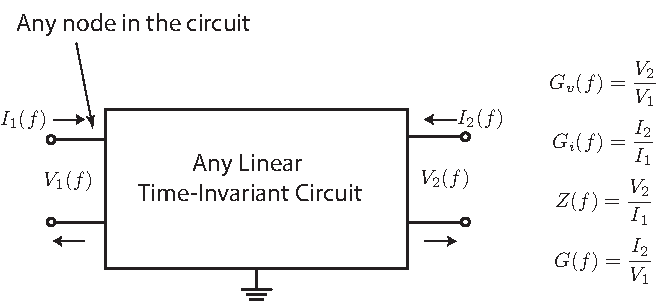
\includegraphics[scale=1]{transfer_func}
\caption{Between two ports in a linear time-invariant (LTI) circuit, we can define four transfer functions.  In this chapter we will focus on the frequency domain transfer functions.}
\label{fig:blackboxltiports}
\end{figure}
%%%%%%%%%%%%%%%%%%%%%%%%%%%%%%%%%%%%%%%%%%%%
%              SUB-SUBSECTION              %
%%%%%%%%%%%%%%%%%%%%%%%%%%%%%%%%%%%%%%%%%%%%
\subsubsection{Example 1 – ECG Amplifier}
The \textbf{electrocardiogram}\index{Amplifier!electrocardiogram} (ECG) is a measurement of the voltage between two points on the body.  For example, as shown in \emph{Fig.~\ref{fig:ecg}}, the voltage across the chest measured from the "right arm" (RA) to the "left arm" (LA) is what's known as lead I.  The ground reference is often the "right leg" (RL).  This voltage is the "input voltage" and we need to amplify it and reject any \textbf{common-mode}\index{Common-mode} noise (see Section~\ref{sec:cmrr}), especially 60 Hz or 50 Hz AC line voltage, which is often orders of magnitude larger than the desired signal.  The output voltage may be single-ended and referenced to a different ground, as shown in the figure.  In this scenario, we define the transfer function as:
    \begin{equation}
        G_v(f) = \frac{V_{out}}{V_1 - V_2 }
    \end{equation}
The variation in frequency is due to the frequency content of the heartbeat signal and possibly filters applied to the signal intentionally to reduce the impact of noise.
%%%%%%%%%%%%%%%%%%%%%%%%%%%%%%%%%%%%%%%%%%%%
%                 FIGURE                   %
%%%%%%%%%%%%%%%%%%%%%%%%%%%%%%%%%%%%%%%%%%%%
\begin{figure}[tb]
\centering
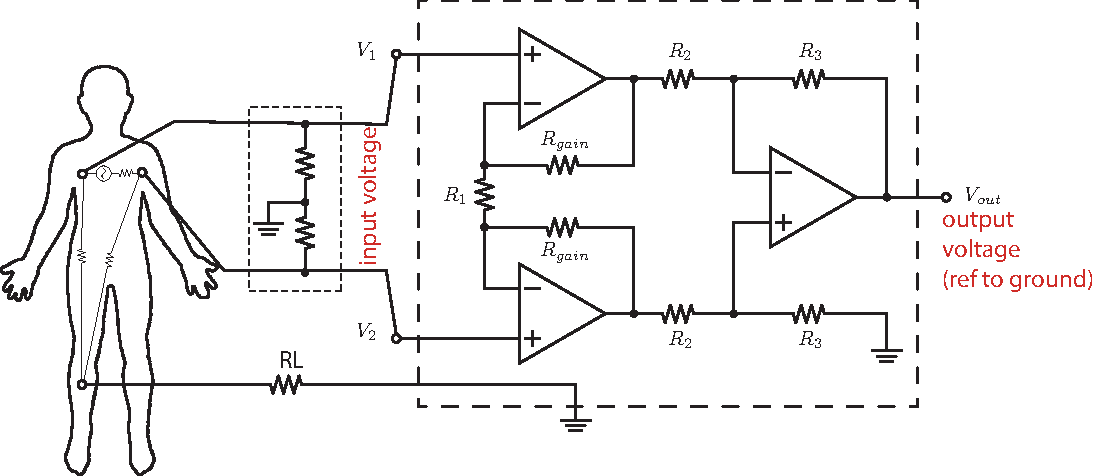
\includegraphics[width=\columnwidth]{ex_opamp-ia2}
\caption{An ECG amplifier is an example of a transfer function from a non-ground referenced port to an output port that is referenced to ground, or a differential to single-ended transfer function.}
\label{fig:ecg}
\end{figure}
%%%%%%%%%%%%%%%%%%%%%%%%%%%%%%%%%%%%%%%%%%%%
%              SUB-SUBSECTION              %
%%%%%%%%%%%%%%%%%%%%%%%%%%%%%%%%%%%%%%%%%%%%
\subsubsection{Example 2 – Mic/Speaker}
%%%%%%%%%%%%%%%%%%%%%%%%%%%%%%%%%%%%%%%%%%%%
%                 FIGURE                   %
%%%%%%%%%%%%%%%%%%%%%%%%%%%%%%%%%%%%%%%%%%%%
\begin{figure}[tb]
\centering
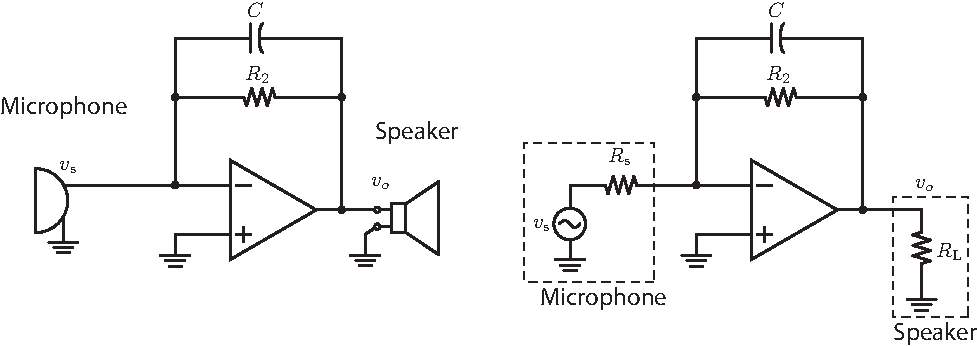
\includegraphics[width=\columnwidth]{ex_microphone}\\
(a)\hspace{8cm}(b)
\caption{The transfer function from a microphone to the output of the amplifier is actually a current to voltage transfer function.  Note the voltage to voltage transfer function is undefined for an ideal op-amp since the negative input terminal is a virtual ground.}
\label{fig:microphone}
\end{figure}
%%%%%%%%%%%%%%%%%%%%%%%%%%%%%%%%%%%%%%%%%%%%
The next example is deceptively simple because on first inspection of \emph{Fig.~\ref{fig:microphone}(a)}, you may conclude that there's an error in the drawing, because the negative input of the inverting amplifier is shorted due to the "virtual ground" connection.  In fact, were it not for the microphone source resistance, as shown in  \emph{Fig.~\ref{fig:microphone}(b)}, this would be the case. But the signal is amplified and filtered by the presence of the capacitor in the inverting amplifier configuration.
\newpage
\noindent
Low frequency signals will see a gain of:
    \begin{equation}
        G_v(f) = \frac{v_{o}}{v_s } = -\frac{R_2}{R_s}
    \end{equation}
On the other hand, very high frequency signals will see a very small gain, because as the capacitor becomes more conductive than the resistor $R_2$, or in other words $\omega C \gg R_2$, then the gain is simply:
    \begin{equation}
        G_v(f) \sim \frac{-\frac{1}{\omega C}}{R_2 } = \frac{-1}{\omega C R_2 }
    \end{equation}
In this example, the presence of the source impedance changed everything.  In general we must be careful to include the potential impact of the source/load impedances.
\newpage
%%%%%%%%%%%%%%%%%%%%%%%%%%%%%%%%%%%%%%%%%%%%
%              SUB-SUBSECTION              %
%%%%%%%%%%%%%%%%%%%%%%%%%%%%%%%%%%%%%%%%%%%%
\subsubsection{Example 3 – Photodetector}
%%%%%%%%%%%%%%%%%%%%%%%%%%%%%%%%%%%%%%%%%%%%
%                 FIGURE                   %
%%%%%%%%%%%%%%%%%%%%%%%%%%%%%%%%%%%%%%%%%%%%
\begin{figure}[t]
\centering
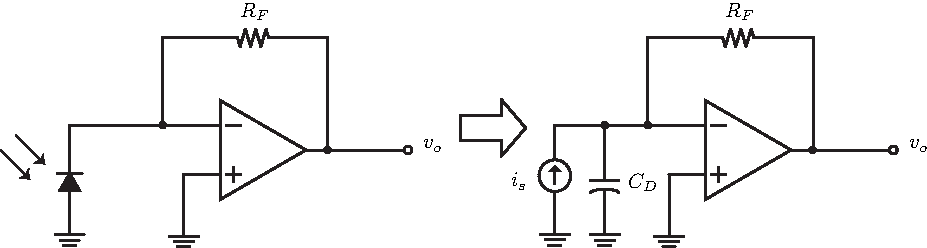
\includegraphics[width=\columnwidth]{ex_photodetect}\\
(a)\hspace{6cm}(b)
\caption{(a) A photodetector is used to convert photons to current, which are then converted into a voltage through the transimpedance amplifier (TIA).  (b) The equivalent circuit model.}
\label{fig:pd_detect}
\end{figure}
%%%%%%%%%%%%%%%%%%%%%%%%%%%%%%%%%%%%%%%%%%%%
For many applications, we need to process a voltage, so a "transimpedance" amplifier is needed to convert the current to the voltage through $R_F$ as shown.\footnote{Why not simply use a resistor in parallel with the diode to convert the current into a voltage?}

Shown in \emph{Fig.~\ref{fig:pd_detect}(a)}, the source is a \textbf{photodiode}\index{Photodiode}, a device that has an output current proportional to the number of impinging photons.  Again, upon first inspection it seems that the diode is "shorted" to ground through the virtual ground connection, but the diode is better modeled as a current source.  The input current is therefore the signal of interest, as shown in \emph{Fig.~\ref{fig:pd_detect}(b)}.  It is important to include the \textbf{source capacitance}\index{Capacitor!source capacitance} ($C_D$), which limits the high frequency performance.  One benefit of the amplifier is that the signal across $C_D$ is mostly shorted, and therefore the impact is not as severe as it would be otherwise.
%%%%%%%%%%%%%%%%%%%%%%%%%%%%%%%%%%%%%%%%%%%%
%             SUBSECTION 2.2.2             %
%%%%%%%%%%%%%%%%%%%%%%%%%%%%%%%%%%%%%%%%%%%%
\subsection{Voltage and Current Gain}
The voltage (current) gain is just the voltage (current) transfer function from one port to another port (see \emph{Fig.~\ref{fig:twoportivgain}}):
    \begin{equation}
        {G_v}(\omega ) = \frac{{{V_2}}}{{{V_1}}} = \left| {\frac{{{V_2}}}{{{V_1}}}} \right|{e^{j({\varphi _2} - {\varphi _1})}}
    \end{equation}
    \begin{equation}
        {G_i}(\omega ) = \frac{{{I_2}}}{{{I_1}}} = \left| {\frac{{{I_2}}}{{{I_1}}}} \right|{e^{j({\varphi _2} - {\varphi _1})}}
    \end{equation}
If \textit{G > }1, the circuit has voltage (current) gain.   If \textit{G} < 1, the circuit has loss or attenuation.   It's a common misconception that only "active" circuits can have gain.  We will demonstrate in \emph{section~\ref{sec:lcr}} that $RCL$ circuits in particular are passive, and can provide voltage and/or current gain.  Another common example is the ubiquitous \textbf{transformer}\index{Transformer}, which provides gain through mutual coupling.  It may surprise you that even $RC$ circuits can provide gain, although not as easily as with inductors and transformers!
%%%%%%%%%%%%%%%%%%%%%%%%%%%%%%%%%%%%%%%%%%%%
%                 FIGURE                   %
%%%%%%%%%%%%%%%%%%%%%%%%%%%%%%%%%%%%%%%%%%%%
\begin{figure}[H]
\centering
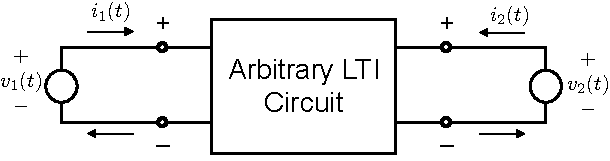
\includegraphics[width=.8\columnwidth]{mod1_3_1_twoport}
\caption{An arbitrary \textbf{two-port}\index{Port models!two-port} consisting of a linear time-invariant circuit.}
\label{fig:twoportivgain}
\end{figure}
%%%%%%%%%%%%%%%%%%%%%%%%%%%%%%%%%%%%%%%%%%%%
\newpage
%%%%%%%%%%%%%%%%%%%%%%%%%%%%%%%%%%%%%%%%%%%%
%             SUBSECTION 2.2.3             %
%%%%%%%%%%%%%%%%%%%%%%%%%%%%%%%%%%%%%%%%%%%%
\subsection{Trans-Impedance and Trans-Admittance}
Current/voltage gain are unitless quantities, but we can define a signal as a voltage or a current, or both (or even a power, or the product).   If the transfer involves voltage to current or vice versa, we must be careful to define the units.  We have a \textbf{trans-impedance}\index{Amplifier!trans-impedance} (TIA) amplifier gain
    \begin{equation}
        J(\omega ) = \frac{{{V_2}}}{{{I_1}}} = \left| {\frac{{{V_2}}}{{{I_1}}}} \right|{e^{j({\varphi _2} - {\varphi _1})}}  [\Omega ]
    \end{equation}
Less commonly, we have a \textbf{trans-admittance}\index{Amplifier!trans-admittance} (TAA) amplifier:
    \begin{equation}
        K(\omega ) = \frac{{{I_2}}}{{{V_1}}} = \left| {\frac{{{I_2}}}{{{V_1}}}} \right|{e^{j({\varphi _2} - {\varphi _1})}}  [S]
    \end{equation}
%%%%%%%%%%%%%%%%%%%%%%%%%%%%%%%%%%%%%%%%%%%%
%             SUBSECTION 2.2.4             %
%%%%%%%%%%%%%%%%%%%%%%%%%%%%%%%%%%%%%%%%%%%%
\subsection{Impede the Currents!}
%%%%%%%%%%%%%%%%%%%%%%%%%%%%%%%%%%%%%%%%%%%%
%                 FIGURE                   %
%%%%%%%%%%%%%%%%%%%%%%%%%%%%%%%%%%%%%%%%%%%%
\begin{figure}[tb]
\centering
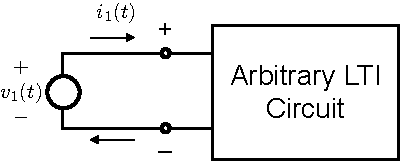
\includegraphics[width=.65\columnwidth]{mod1_3_2_oneport}
\caption{An arbitrary \textbf{one-port}\index{Port models!one-port} linear time-invariant circuit.}
\label{fig:oneport}
\end{figure}
%%%%%%%%%%%%%%%%%%%%%%%%%%%%%%%%%%%%%%%%%%%%
Suppose that the "input" is defined as the voltage of a terminal pair (\textit{port}) and the “output” is defined as the current into the port (see \emph{Fig.~\ref{fig:oneport}}).  
    \begin{equation}
        v(t) = V{e^{j\omega t}} = \left| V \right|{e^{j(\omega t + {\varphi _v})}}
    \end{equation}
    \begin{equation}
        i(t) = I{e^{j\omega t}} = \left| I \right|{e^{j(\omega t + {\varphi _i})}}
    \end{equation}
The \textbf{impedance}\index{Impedance} $Z$ is defined as the ratio of the phasor voltage to phasor current (“self” transfer function):
    \begin{equation}
        Z(\omega ) = H(\omega ) = \frac{V}{I} = \left| {\frac{V}{I}} \right|{e^{j({\varphi _v} - {\varphi _i})}}
    \end{equation}
We are of course familiar with the concept of impedance $Z$, but even though we may not think about it as a transfer function, it is indeed a transfer function.
%%%%%%%%%%%%%%%%%%%%%%%%%%%%%%%%%%%%%%%%%%%%
%             SUBSECTION 2.2.5             %
%%%%%%%%%%%%%%%%%%%%%%%%%%%%%%%%%%%%%%%%%%%%
\subsection{Admit the Currents!}
Similarly, suppose that the "input" is defined as the current of a terminal pair (port) and the “output” is defined as the voltage into the port. The \textbf{admmittance}\index{Admittance} $Y$ is defined as the ratio of the current to voltage (“self” transfer function)
    \begin{equation}
        Y(\omega ) = H(\omega ) = \frac{I}{V} = \left| {\frac{I}{V}} \right|{e^{j({\varphi _i} - {\varphi _v})}}
    \end{equation}
%%%%%%%%%%%%%%%%%%%%%%%%%%%%%%%%%%%%%%%%%%%%%%%%%%%%%%%%%%%%%%%%%%%%%%%%%%%%%%%%%%%%%%%%
%%%%%%%%%%%%%%%%%%%%%%%%%%%%%%%%%%%%%%%%%%%%%%%%%%%%%%%%%%%%%%%%%%%%%%%%%%%%%%%%%%%%%%%%
%                                   SECTION 2.3                                        %
%%%%%%%%%%%%%%%%%%%%%%%%%%%%%%%%%%%%%%%%%%%%%%%%%%%%%%%%%%%%%%%%%%%%%%%%%%%%%%%%%%%%%%%%
%%%%%%%%%%%%%%%%%%%%%%%%%%%%%%%%%%%%%%%%%%%%%%%%%%%%%%%%%%%%%%%%%%%%%%%%%%%%%%%%%%%%%%%%
\section{Transfer Function Poles/Zeros}
%%%%%%%%%%%%%%%%%%%%%%%%%%%%%%%%%%%%%%%%%%%%
%             SUBSECTION 2.3.1             %
%%%%%%%%%%%%%%%%%%%%%%%%%%%%%%%%%%%%%%%%%%%%
\subsection{Complex Transfer Function}
Following our derivation from the last chapter, we excite a system with an input voltage (current) \textit{x} and define the output voltage \textit{y} (current) to be any node voltage (branch current).  For a complex exponential input, the "transfer function" from input to output is given by:
    \begin{equation}
        H \equiv \frac{y}{x} = \left( {a + {b_1}j\omega  + {b_2}{{(j\omega )}^2} +  \cdots  + \frac{{{c_1}}}{{j\omega }} + \frac{{{c_2}}}{{{{(j\omega )}^2}}} +  \cdots } \right)
    \end{equation}
 We can write this in \textbf{canonical form}\index{Transfer function!canonical form} as a rational function:
    \begin{equation}
        H(\omega ) = \frac{{{n_1} + {n_2}j\omega  + {n_3}{{(j\omega )}^2} +  \cdots }}{{{d_1} + {d_2}j\omega  + {d_3}{{(j\omega )}^2} +  \cdots }}
    \end{equation}
This form of the equation shows that the numerator and denominator are in general polynomial equations, and polynomial equations are characterized by either their coefficients or more importantly their roots.
%%%%%%%%%%%%%%%%%%%%%%%%%%%%%%%%%%%%%%%%%%%%
%              SUB-SUBSECTION              %
%%%%%%%%%%%%%%%%%%%%%%%%%%%%%%%%%%%%%%%%%%%%
\subsubsection{“s” Complex Plane}
You may hear people talking about transfer functions as a function of complex “s” rather than frequency
\begin{equation}
	H(s) = \frac{{({z_1} - s)({z_2} - s) \cdots }}{{({p_1} - s)({p_2} - s) \cdots }}
\end{equation}
As we learned, this is a generalization (Laplace domain\index{Laplace domain}) of frequency. When doing AC analysis, we are deriving the function along the imaginary axis (sinusoidal steady-state response)
\begin{equation}
	H(s = j\omega ) = \frac{{({z_1} - j\omega )({z_2} - j\omega ) \cdots }}{{({p_1} - j\omega )({p_2} - j\omega ) \cdots }}
\end{equation}
This is why you may see introduce this notation:  $H(j\omega )$
%%%%%%%%%%%%%%%%%%%%%%%%%%%%%%%%%%%%%%%%%%%%
%             SUBSECTION 2.3.2             %
%%%%%%%%%%%%%%%%%%%%%%%%%%%%%%%%%%%%%%%%%%%%
\subsection{Poles and Zeros}
For most circuits that we deal with, the transfer function can be shown to be a \textbf{rational function}\index{Transfer function!rational form}:
\begin{equation}
	H(\omega ) = \frac{{{n_1} + {n_2}j\omega  + {n_3}{{(j\omega )}^2} +  \cdots }}{{{d_1} + {d_2}j\omega  + {d_3}{{(j\omega )}^2} +  \cdots }}
\end{equation}
The behavior of the circuit can be extracted by putting the transfer function into \textbf{standard form}\index{Transfer function!standard form}, and finding the roots of the numerator and denominator:
\begin{equation} 
	H(\omega ) = \frac{{({z_1} - j\omega )({z_2} - j\omega ) \cdots }}{{({p_1} - j\omega )({p_2} - j\omega ) \cdots }} = \frac{{\prod {({z_i} - j\omega )} }}{{\prod {({p_i} - j\omega )} }}
\end{equation}
Or in another form (\textbf{DC gain explicit}\index{Transfer function!DC gain form}):
\begin{equation}
	H(\omega ) = {G_0}{(j\omega )^K}\frac{{(1 - j\omega {\tau _{z1}})(1 - j\omega {\tau _{z2}}) \cdots }}{{(1 - j\omega {\tau _{p2}})(1 - j\omega {\tau _{p2}}) \cdots }}
\end{equation}	
\begin{equation} = {G_0}{(j\omega )^K}\frac{{\prod {(1 - j\omega {\tau _{z,i}})} }}{{\prod {(1 - j\omega {\tau _{p,i}})} }}
\end{equation}
%%%%%%%%%%%%%%%%%%%%%%%%%%%%%%%%%%%%%%%%%%%%
%              SUB-SUBSECTION              %
%%%%%%%%%%%%%%%%%%%%%%%%%%%%%%%%%%%%%%%%%%%%
\subsubsection{Building Tents: Poles and Zeros}
The roots of the numerator are called the \textbf{“zeros”}\index{Transfer function!zeros} since at these frequencies, the transfer function is zero.  These are the "stakes in the ground" of our tent, see \emph{Fig.~\ref{fig:tent}}.  The roots of the denominator are called the \textbf{“poles”}\index{Transfer function!poles}, since at these frequencies the transfer function peaks (like a pole in a tent).
%%%%%%%%%%%%%%%%%%%%%%%%%%%%%%%%%%%%%%%%%%%%
%                 FIGURE                   %
%%%%%%%%%%%%%%%%%%%%%%%%%%%%%%%%%%%%%%%%%%%%
\begin{figure}[tb]
\centering
\includegraphics[angle=-0.0,width=.8\columnwidth]{image_11.jpg}
\caption{A tent has poles and "zeros", or locations of stakes.  At the stakes the elevation is at ground (zero), whereas at the poles the elevation hits a local maximum.}
\label{fig:tent}
\end{figure}
%%%%%%%%%%%%%%%%%%%%%%%%%%%%%%%%%%%%%%%%%%%%
While the frequency response requires us to keep track of the transfer function over a continuous frequency spectrum, this perspective gives us a new insight.  We actually can completely characterize a system by a finite number of poles and zeros.  Come to think of it, this should be obvious because our circuit is built out of a finite number of components ($L$, $C$, $M$, and dependent sources).  So the number of poles and zeros should be related to the number of elements with "memory", such as inductors and capacitors.  
%%%%%%%%%%%%%%%%%%%%%%%%%%%%%%%%%%%%%%%%%%%%%%%%%%%%%%%%%%%%%%%%%%%%%%%%%%%%%%%%%%%%%%%%
%%%%%%%%%%%%%%%%%%%%%%%%%%%%%%%%%%%%%%%%%%%%%%%%%%%%%%%%%%%%%%%%%%%%%%%%%%%%%%%%%%%%%%%%
%                                   SECTION 2.4                                        %
%%%%%%%%%%%%%%%%%%%%%%%%%%%%%%%%%%%%%%%%%%%%%%%%%%%%%%%%%%%%%%%%%%%%%%%%%%%%%%%%%%%%%%%%
%%%%%%%%%%%%%%%%%%%%%%%%%%%%%%%%%%%%%%%%%%%%%%%%%%%%%%%%%%%%%%%%%%%%%%%%%%%%%%%%%%%%%%%%
\section{AC Circuits Review}
%%%%%%%%%%%%%%%%%%%%%%%%%%%%%%%%%%%%%%%%%%%%
%             SUBSECTION 2.4.1             %
%%%%%%%%%%%%%%%%%%%%%%%%%%%%%%%%%%%%%%%%%%%%
\subsection{Phasors}
With our new confidence in complex numbers, we can go full steam ahead and work with them directly.  We can even drop the time factor, $e^{j\omega t}$, since it will cancel out of the equations.  In other words, the part that matters is the amplitude and phase shift of the resulting complex exponential, not the complex exponential itself.  Let's define this part as the \textbf{"phasor"}\index{Phasors}.
%%%%%%%%%%%%%%%%%%%%%%%%%%%%%%%%%%%%%%%%%%%%
We excite system with a phasor: ${\tilde V_1} = {V_1}{e^{j{\varphi _1}}}$ and the response  will also be phasor: ${\tilde V_2} = {V_2}{e^{j{\varphi _2}}}$.   
%%%%%%%%%%%%%%%%%%%%%%%%%%%%%%%%%%%%%%%%%%%%
%                 FIGURE                   %
%%%%%%%%%%%%%%%%%%%%%%%%%%%%%%%%%%%%%%%%%%%%
\begin{figure}[H]
\centering
\begin{tabular}{ccc}
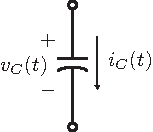
\includegraphics[width=.35\columnwidth]{mod1_3_3_cap} & \hspace{1cm} &
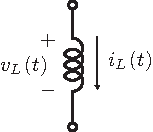
\includegraphics[width=.35\columnwidth]{mod1_3_4_ind}\\
(a) & & (b)\\
\end{tabular}
\caption{(a) Capacitor and (b) inductor  $I$-$V$ relations in the time domain.}
\label{fig:lcphasor}
\end{figure}
%%%%%%%%%%%%%%%%%%%%%%%%%%%%%%%%%%%%%%%%%%%%
%             SUBSECTION 2.4.2             %
%%%%%%%%%%%%%%%%%%%%%%%%%%%%%%%%%%%%%%%%%%%%
\subsection{Capacitor I-V Phasor Relation}
To find the phasor relation for current and voltage for a capacitor, begin with the "$I-V$" relation in the time domain (see \emph{Fig.~\ref{fig:lcphasor}}):
    \begin{equation}
        {i_c}(t) = C\frac{{d{v_C}(t)}}{{dt}}
    \end{equation}
Now for sinusoidal steady state we substitute:
    \begin{equation}
        {i_c}(t) = {I_c}{e^{j\omega t}}
    \end{equation}
and,
    \begin{equation}
        {v_c}(t) = {V_c}{e^{j\omega t}}
    \end{equation}
This leads to:
    \begin{equation}
        {I_c}{e^{j\omega t}} = C\frac{d}{{dt}}[{V_c}{e^{j\omega t}}]
    \end{equation}
or,
    \begin{equation}
        C{V_c}\frac{d}{{dt}}{e^{j\omega t}} = j\omega \,C{V_c}{e^{j\omega t}}
    \end{equation}
Let's eliminate the common $e^{j\omega t}$ factor:
    \begin{equation}
        {I_c}{e^{j\omega t}} = j\omega \,C{V_c}{e^{j\omega t}}
    \end{equation}
Or more simply, the phasor relation:
    \begin{equation}
        {I_c} = j\omega \,C\,{V_c}
    \end{equation}
This is \textbf{"Ohm's law"}\index{Ohm's law} in the frequency-domain\index{Frequency-domain} for a capacitor.
\newpage
%%%%%%%%%%%%%%%%%%%%%%%%%%%%%%%%%%%%%%%%%%%%
%             SUBSECTION 2.4.3             %
%%%%%%%%%%%%%%%%%%%%%%%%%%%%%%%%%%%%%%%%%%%%
\subsection{Inductor I-V Phasor Relation}
Let's now find the phasor relation for current and voltage in an inductor using the same procedure:
    \begin{equation}
        v(t) = L\frac{{di(t)}}{{dt}}
    \end{equation} 
For sinusoidal steady-state, this implies:
    \begin{equation}
        V{e^{j\omega t}} = L\frac{d}{{dt}}[I{e^{j\omega t}}]
    \end{equation}
or,
    \begin{equation}
        LI\frac{d}{{dt}}{e^{j\omega t}} = j\omega \,LI{e^{j\omega t}}
    \end{equation}
Canceling the common factor:
    \begin{equation}
        V{e^{j\omega t}} = j\omega \,LI{e^{j\omega t}}
    \end{equation}
This is the phasor relation for an inductor, or "Ohm's Law" in the frequency domain for an inductor:
    \begin{equation}
        V = j\omega \,L\,I
    \end{equation}
%%%%%%%%%%%%%%%%%%%%%%%%%%%%%%%%%%%%%%%%%%%%
%             SUBSECTION 2.4.4             %
%%%%%%%%%%%%%%%%%%%%%%%%%%%%%%%%%%%%%%%%%%%%
\subsection{Direct Calculation of \textit{H} (no DEs)}
To directly calculate the transfer function (impedance, trans-impedance, etc) we can generalize the circuit analysis concept from the “real” domain to the “phasor” domain.   We drop the time dependence $e^{j\omega t}$ (common factor that cancels out) and just keep track of amplitude and phase (phasor).  With the concept of \textbf{impedance}\index{Impedance} (\textbf{admittance}\index{Admittance}), we directly analyze a circuit without explicitly writing down any differential equations.  We are free to use KVL, KCL, mesh analysis, loop analysis, or nodal analysis where inductors and capacitors are treated as complex resistors, or more correctly as an impedance (or admittance).
\newpage
%%%%%%%%%%%%%%%%%%%%%%%%%%%%%%%%%%%%%%%%%%%%
%                 FIGURE                   %
%%%%%%%%%%%%%%%%%%%%%%%%%%%%%%%%%%%%%%%%%%%%
\begin{figure}[t]
\centering
\begin{tabular}{cc}
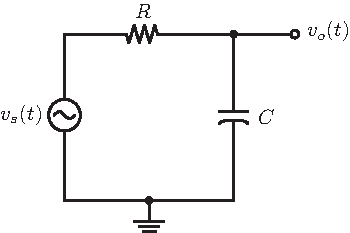
\includegraphics[angle=-0.0,scale=1]{mod1_3_5_rc_lpf} &
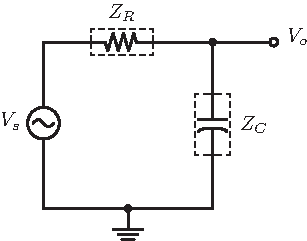
\includegraphics[angle=-0.0,scale=1]{mod1_3_6_rc_lpf_Z}\\
(a) & (b)\\
\end{tabular}
\caption{(a) The low-pass filter in the time domain and (b) an AC equivalent circuit.}
\label{fig:lpfagain}
\end{figure}
%%%%%%%%%%%%%%%%%%%%%%%%%%%%%%%%%%%%%%%%%%%%%%%%%%%%%%%%%%%%%%%%%%%%%%%%%%%%%%%%%%%%%%%%
%%%%%%%%%%%%%%%%%%%%%%%%%%%%%%%%%%%%%%%%%%%%%%%%%%%%%%%%%%%%%%%%%%%%%%%%%%%%%%%%%%%%%%%%
%                                   SECTION 2.5                                        %
%%%%%%%%%%%%%%%%%%%%%%%%%%%%%%%%%%%%%%%%%%%%%%%%%%%%%%%%%%%%%%%%%%%%%%%%%%%%%%%%%%%%%%%%
%%%%%%%%%%%%%%%%%%%%%%%%%%%%%%%%%%%%%%%%%%%%%%%%%%%%%%%%%%%%%%%%%%%%%%%%%%%%%%%%%%%%%%%%
\section{Example AC Circuit Problems}
%%%%%%%%%%%%%%%%%%%%%%%%%%%%%%%%%%%%%%%%%%%%
%             SUBSECTION 2.5.1             %
%%%%%%%%%%%%%%%%%%%%%%%%%%%%%%%%%%%%%%%%%%%%
\subsection{LPF Example: Again!}
In \emph{Fig.~\ref{fig:lpfagain}}, we show a "real"  time-domain circuit and the corresponding frequency-domain “phasor” circuit.   Instead of setting up the DE in the time-domain, we prefer to do calculations directly in the frequency domain using phasors, treating the capacitor as an imaginary "resistance" or impedance.  We know the impedances: ${Z_R} = R $ and $ {Z_C} = \frac{1}{{j\omega C}}$.

The fastest way to solve the problem is to say that the LPF is really a \textbf{voltage divider}\index{Voltage divider}:
    \begin{equation}
        H(\omega) = \frac{V_o}{V_s} = \frac{Z_C}{Z_C + Z_R}
        = \frac{\frac{1}{j\,\omega\,C}}{R + \frac{1}{j\,\omega\,C}} = \frac{1}{1 + j\,\omega\,R\,C}
    \end{equation}
%%%%%%%%%%%%%%%%%%%%%%%%%%%%%%%%%%%%%%%%%%%%
%             SUBSECTION 2.5.2             %
%%%%%%%%%%%%%%%%%%%%%%%%%%%%%%%%%%%%%%%%%%%%
\subsection{Bigger Example (no problem!)}
Consider a more complicated example shown in \emph{Fig.~\ref{fig:bigexample}}.  To find $v_o$, you can do \textbf{nodal analysis}\index{Nodal analysis} or use \textbf{network theorems}\index{Network theorems} to simplify the circuit.  Let's find the \textbf{Thévenin equivalent}\index{Thévenin equivalent} from $C_2$'s perspective.  The open-circuit voltage is just the first voltage divider:
    \begin{equation}
        v_{th} = \frac{Z_{C_1}}{R_1 + Z_{C_1}}\,v_s 
    \end{equation}
The impedance looking into the circuit from $C_2$ is given by:
    \begin{equation}
        Z_{th} = R_2 + R_1 \big|\big| Z_{C_1}
    \end{equation}
Therefore we have:
    \begin{equation}
        v_o = \frac{Z_{C_2}}{Z_{C_2} + Z_{th}} V_{th} 
    \end{equation}
%%%%%%%%%%%%%%%%%%%%%%%%%%%%%%%%%%%%%%%%%%%%
%                 FIGURE                   %
%%%%%%%%%%%%%%%%%%%%%%%%%%%%%%%%%%%%%%%%%%%%
\begin{figure}[H]
\centering
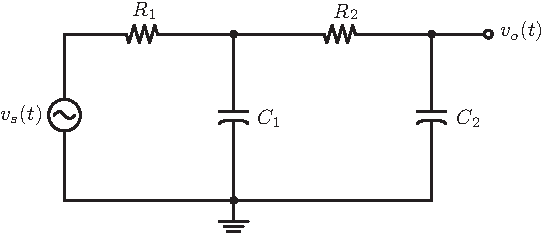
\includegraphics[angle=-0.0,scale=1]{mod1_3_7_rc_lpf2}
\caption{A circuit with two resistors and two capacitors can be analyzed quickly using nodal analysis or circuit theorems by treating the capacitors as impedances.}
\label{fig:bigexample}
\end{figure}
%%%%%%%%%%%%%%%%%%%%%%%%%%%%%%%%%%%%%%%%%%%%
\newpage
%%%%%%%%%%%%%%%%%%%%%%%%%%%%%%%%%%%%%%%%%%%%
%                 FIGURE                   %
%%%%%%%%%%%%%%%%%%%%%%%%%%%%%%%%%%%%%%%%%%%%
\begin{figure}[t]
\centering
\includegraphics[scale=1]{rlc}
\caption{A series $RLC$ circuit.}
\label{fig:rlc}
\end{figure}
%%%%%%%%%%%%%%%%%%%%%%%%%%%%%%%%%%%%%%%%%%%%
%             SUBSECTION 2.5.3             %
%%%%%%%%%%%%%%%%%%%%%%%%%%%%%%%%%%%%%%%%%%%%
\subsection{Series RLC Circuits} \label{sec:lcr}
The $RLC$ circuit shown in \emph{Fig.~\ref{fig:rlc}} is simple but extremely useful and rich in application.  Since the circuit elements are all in series, the \textbf{input impedance}\index{Impedance!Input impedance} seen by the source is simply given by:
    \begin{align*}
        Z &= j\omega L + \frac{1}{j\omega C} + R\\
        &= R + j\omega L + \frac{j\omega L}{j^2{\omega}^2 LC}\\
        &= R + j\omega L \left( 1 - \frac{1}{\omega^2 LC}\right)
    \end{align*}
The impedance is purely real at at the \textbf{resonant frequency}\index{Resonant frequency}, or when $\Im(Z) = 0$, which happens at a frequency $\omega = \pm \frac{1}{\sqrt{L C}}$.  At resonance the impedance takes on a minimal value.  See \emph{Fig.~\ref{fig:rlcphasor}} for phasor diagrams of resonance, including before and after resonance occurs.
%%%%%%%%%%%%%%%%%%%%%%%%%%%%%%%%%%%%%%%%%%%%
%                 FIGURE                   %
%%%%%%%%%%%%%%%%%%%%%%%%%%%%%%%%%%%%%%%%%%%%
\begin{figure}[H]
\centering
\includegraphics[scale=.95]{rlcphasor}\\
(a)\hspace{3.5cm}(b)\hspace{3.3cm}(c)
\caption{The phasor diagram shows the relations between the voltages across each component.  Note that the inductor/capacitor voltages are exactly $180^\circ$ degrees out of phase.  (a) Below resonance, the reactance of the capacitor dominates.  (b) At resonance, these reactances are equal and so the voltages across the circuit sum to $v_R$, so the entire source voltage is applied to the resistor $R$.  (c) Above resonance, the reactance of the inductor dominates.}
\label{fig:rlcphasor}
\end{figure}
%%%%%%%%%%%%%%%%%%%%%%%%%%%%%%%%%%%%%%%%%%%%
\newpage
%%%%%%%%%%%%%%%%%%%%%%%%%%%%%%%%%%%%%%%%%%%%
%              SUB-SUBSECTION              %
%%%%%%%%%%%%%%%%%%%%%%%%%%%%%%%%%%%%%%%%%%%%
\subsubsection{Series Resonance}
It is worthwhile to investigate the cause of resonance, or the cancellation of the reactive components due to the inductor and capacitor.  Since the inductor and capacitor voltages are always $180^\circ$ out of phase, and one reactance is dropping while the other is increasing, there is clearly always a frequency when the magnitudes are equal.  Resonance, defined as $\omega_0$, occurs when $\omega L = \frac{1}{\omega C}$.  Now we define the resonant frequency of this circuit as:
    \begin{equation}
        \omega_0 = \frac{1}{LC}
    \end{equation}
%%%%%%%%%%%%%%%%%%%%%%%%%%%%%%%%%%%%%%%%%%%%
%              SUB-SUBSECTION              %
%%%%%%%%%%%%%%%%%%%%%%%%%%%%%%%%%%%%%%%%%%%%
\subsubsection{Quality Factor}
So what is the magic about this circuit?  The first observation is that at resonance, the voltage across the reactances can be larger, in fact much larger, than the voltage across the resistors $R$ (again, see \emph{Fig.~\ref{fig:rlcphasor}} and observe the length of the vectors).  In other words, this circuit has \textbf{voltage gain}\index{Gain!voltage}.  Of course it does not have \textbf{power gain}\index{Gain!power}, for it is a \textbf{passive circuit}\index{Passive circuit} after all.  The voltage across the inductor is given by:
    \begin{equation}
        v_L = j\omega_0 L i = j\omega_0 L \frac{v_s}{Z(j\omega_0)} =  j\omega_0 L \frac{v_s}{R} = j Q \times v_s
    \end{equation}
where we have defined a circuit \textbf{Q (quality) factor}\index{Quality/Q factor} at resonance as:
    \begin{equation}
        Q = \frac{\omega_0 L}{R}
    \end{equation}
%%%%%%%%%%%%%%%%%%%%%%%%%%%%%%%%%%%%%%%%%%%%
%              SUB-SUBSECTION              %
%%%%%%%%%%%%%%%%%%%%%%%%%%%%%%%%%%%%%%%%%%%%
\subsubsection{Voltage Multiplication}
It's easy to show that the same voltage multiplication occurs across the capacitor (the reactances are equal at resonance after all)
    \begin{equation}
        v_C = \frac{1}{j\omega_0 C} i = \frac{1}{j\omega_0 C}
        \frac{v_s}{Z(j\omega_0)} = \frac{1}{j\omega_0 R C} \frac{v_s}{R} = - j Q
        \times v_s
    \end{equation}
This voltage multiplication property is the key feature of the circuit that allows it to be used as an \textbf{impedance transformer}\index{Transformer!impedance}.\footnote{It is important to distinguish this $Q$ factor from the intrinsic $Q$ of the inductor and capacitor.  For now, we assume the inductor and capacitor are ideal.}
%%%%%%%%%%%%%%%%%%%%%%%%%%%%%%%%%%%%%%%%%%%%
%              SUB-SUBSECTION              %
%%%%%%%%%%%%%%%%%%%%%%%%%%%%%%%%%%%%%%%%%%%%
\subsubsection{More of Q}
We can re-write the $Q$ factor in several equivalent forms owing to the equality of the reactances at resonance
    \begin{equation} \label{eq:qdefs}
        Q = \frac{\omega_0 L}{R} = \frac{1}{\omega_0 C} \frac{1}{R} = \frac{\sqrt{LC}}{C} \frac{1}{R} = \sqrt{\frac{L}{C}} \frac{1}{R} = \frac{Z_0}{R}
    \end{equation}
where we have defined the $Z_0 = \sqrt{\tfrac{L}{C}}$ as the characteristic impedance of the circuit.
%%%%%%%%%%%%%%%%%%%%%%%%%%%%%%%%%%%%%%%%%%%%
%              SUB-SUBSECTION              %
%%%%%%%%%%%%%%%%%%%%%%%%%%%%%%%%%%%%%%%%%%%%
\subsubsection{Resonant Circuit Transfer Function}
Let's now examine the transfer function\index{Transfer function} of the circuit.  Combining $L$ and $C$ as a series impedance, we have a simple voltage divider\index{Voltage divider}:
\begin{equation}
    H(j\omega) = \frac{v_o}{v_s} = \frac{R}{j\omega L + \frac{1}{j\omega C} +
      R}
\end{equation}
\begin{equation}
    H(j\omega) = \frac{j\omega R C }{1 - \omega^2 LC + j\omega R C}
\end{equation}
Obviously, the circuit cannot conduct DC current, so there is a zero\index{Transfer function!zeros} in the transfer function.  The denominator is a quadratic polynomial.  It is worthwhile to put it into a standard form\index{Transfer function!standard form} that quickly reveals important circuit parameters:
    \begin{equation}
        H(j\omega) = \frac{j\omega \frac{R}{L} }{\frac{1}{LC} + (j\omega)^2 + j\omega \frac{R}{L}}
    \end{equation}
Using the definition of $Q$ and $\omega_0$ for the circuit:
    \begin{equation}
        H(j\omega) = \frac{j\omega \frac{\omega_0}{Q} }{\omega_0^2 +  (j\omega)^2 + j \frac{\omega\omega_0}{Q}}
    \end{equation}
Factoring the denominator with the assumption that $Q > \omega$ gives us the complex poles of the circuit:
    \begin{equation}
        s^\pm = -\frac{\omega_0}{2 Q} \pm j\omega_0 \sqrt{1 - \frac{1}{4Q^2}}
    \end{equation}
The poles have a constant magnitude equal to the resonant frequency:
    \begin{equation}
        |s| = \sqrt{\cancel{\frac{\omega_0^2}{4 Q^2}} + \omega_0^2 \left(1 - \cancel{\frac{1}{4Q^2}} \right)} = \omega_0
    \end{equation}
%%%%%%%%%%%%%%%%%%%%%%%%%%%%%%%%%%%%%%%%%%%%
%              SUB-SUBSECTION              %
%%%%%%%%%%%%%%%%%%%%%%%%%%%%%%%%%%%%%%%%%%%%
\subsubsection{Circuit Bandwidth and Selectivity}
%%%%%%%%%%%%%%%%%%%%%%%%%%%%%%%%%%%%%%%%%%%%
%                 FIGURE                   %
%%%%%%%%%%%%%%%%%%%%%%%%%%%%%%%%%%%%%%%%%%%%
\begin{figure}[t]
\centering
\includegraphics[width=.65\columnwidth]{transferrlc}
\caption{The transfer function from source to the resistor voltage as a function of frequency.  Depending on the component values (circuit $Q$), the transfer function exhibits either low or high selectivity.} \label{fig:transferrlc}
\end{figure}
%%%%%%%%%%%%%%%%%%%%%%%%%%%%%%%%%%%%%%%%%%%%
As we plot the magnitude of the transfer function (\emph{Fig.~\ref{fig:transferrlc}}), we see that the selectivity of the circuit is also related inversely to the $Q$ factor.  

In the limit that $Q \rightarrow \infty$, the circuit is infinitely selective and only allows signals at resonance $\omega_0$ to travel to the load.  Note that the peak gain in the circuit is always unity, regardless of $Q$, since at resonance the $L$ and $C$ together disappear and effectively all the source voltage appears across the load.  The selectivity of the circuit lends itself well to filter applications.  To characterize the peakiness, let's compute the frequency when the magnitude squared of the transfer function drops by half:
    \begin{equation}
        | H(j\omega)|^2 = \frac{ \left(\omega \frac{\omega_0}{Q} \right)^2}{\left( \omega_0^2 - \omega^2\right)^2 + \left( \omega \frac{\omega_0}{Q}\right)^2} = \frac{1}{2}
    \end{equation}
This happens when:
    \begin{equation}
        \left( \frac{\omega_0^2 - \omega^2}{\omega_0\omega / Q}\right)^2 = 1
    \end{equation}
Solving the above equation yields four solutions, corresponding to two positive and two negative frequencies.  The peakiness is characterized by the difference between these frequencies, or the bandwidth\index{Bandwidth}, given by:
    \begin{equation} \label{eq:3db}
        \Delta\omega = \omega_+ - \omega_- = \frac{\omega_0}{Q}
    \end{equation}
The normalized bandwidth is inversely proportional to the circuit $Q$:
    \begin{equation}
        \frac{\Delta\omega}{\omega_0} =\frac{1}{Q}
    \end{equation}
You can also show that the resonance frequency is the geometric mean frequency of the $3$~dB frequencies:
    \begin{equation}
        \omega_0 = \sqrt{\omega_+ \omega_-}
    \end{equation}
%%%%%%%%%%%%%%%%%%%%%%%%%%%%%%%%%%%%%%%%%%%%%%%%%%%%%%%%%%%%%%%%%%%%%%%%%%%%%%%%%%%%%%%%
%%%%%%%%%%%%%%%%%%%%%%%%%%%%%%%%%%%%%%%%%%%%%%%%%%%%%%%%%%%%%%%%%%%%%%%%%%%%%%%%%%%%%%%%
%                                   SECTION 2.6                                        %
%%%%%%%%%%%%%%%%%%%%%%%%%%%%%%%%%%%%%%%%%%%%%%%%%%%%%%%%%%%%%%%%%%%%%%%%%%%%%%%%%%%%%%%%
%%%%%%%%%%%%%%%%%%%%%%%%%%%%%%%%%%%%%%%%%%%%%%%%%%%%%%%%%%%%%%%%%%%%%%%%%%%%%%%%%%%%%%%%
\section{Bode Plots}
%%%%%%%%%%%%%%%%%%%%%%%%%%%%%%%%%%%%%%%%%%%%
%             SUBSECTION 2.6.1             %
%%%%%%%%%%%%%%%%%%%%%%%%%%%%%%%%%%%%%%%%%%%%
\subsection{Finding the Magnitude and Phase (Quickly!)}
The magnitude of the response can be calculated quickly by using the property of the mag operator:
    \begin{equation}
        \left| {H(\omega )} \right| =
            \left| {{G_0}{{(j\omega )}^K} \frac{{(1 - j\omega {\tau _{z1}})(1 - j\omega {\tau _{z2}}) \cdots }}{{(1 - j\omega {\tau _{p2}})(1 - j\omega {\tau _{p2}}) \cdots }}} \right|
    \end{equation}
Separating out the terms:
    \begin{equation}
        = \left| {{G_0}} \right|{\omega ^K} \frac{{\left| {1 - j\omega {\tau _{z1}}} \right|\left| {1 - j\omega {\tau _{z2}}} \right| \cdots }} {{\left| {1 - j\omega {\tau _{p2}}} \right|\left| {1 - j\omega {\tau _{p2}}} \right| \cdots}}
    \end{equation}
The magnitude at DC depends on $G_0$  and the number of poles/zeros at DC. If $K > 0$,  the DC gain is zero. If $K < 0$, DC gain is infinite. Otherwise if $K = 0$, then DC gain is simply $G_0$.
The phase can be computed quickly with the following formula:
    \begin{equation}
        \angle H(\omega ) = \angle {G_0}{(j\omega )^K}\frac{{(1 - j\omega {\tau _{z1}})(1 - j\omega {\tau _{z2}}) \cdots }}{{(1 - j\omega {\tau _{p2}})(1 - j\omega {\tau _{p2}}) \cdots }}
    \end{equation}
Using the properties of the phase operator:
    \begin{equation}
        = \angle {G_0} + \angle {(j\omega )^K} + \angle (1 - j\omega {\tau _{z1}}) + \angle (1 - j\omega {\tau _{z2}}) + \cdots - \angle (1 - j\omega {\tau _{p1}}) - \angle (1 - j\omega {\tau _{p2}}) - \cdots
    \end{equation}
Note that the second term is simple to calculate for positive frequencies:
    \begin{equation}
        \angle {(j\omega )^K} = K\frac{\pi}{2}
    \end{equation}
Interpret this as saying that multiplication by \textit{j} is equivalent to rotation by 90 degrees.
%%%%%%%%%%%%%%%%%%%%%%%%%%%%%%%%%%%%%%%%%%%%
%             SUBSECTION 2.6.2             %
%%%%%%%%%%%%%%%%%%%%%%%%%%%%%%%%%%%%%%%%%%%%
\subsection{Bode Plot}
%%%%%%%%%%%%%%%%%%%%%%%%%%%%%%%%%%%%%%%%%%%%
%                 FIGURE                   %
%%%%%%%%%%%%%%%%%%%%%%%%%%%%%%%%%%%%%%%%%%%%
%\begin{figure}[tb]
%\begin{center}
%\includegraphics[angle=-0.0,width=.75\columnwidth]{dB3}
%\end{center}
%\caption{x}
%\label{fig:x}
%\end{figure}
%%%%%%%%%%%%%%%%%%%%%%%%%%%%%%%%%%%%%%%%%%%%
A \textbf{Bode Plot}\index{Bode plot} is simply a "sketch" of the $\log$-$\log$ plot of the magnitude and phase response of a circuit (impedance, transimpedance, gain, ...).  It provides insight into the behavior of a circuit as a function of frequency without detailed calculations.  The $\log$ expands the scale so that breakpoints in the transfer function are clearly delineated.  In feedback circuit design, Bode plots are used to “compensate” circuits for stability.
%%%%%%%%%%%%%%%%%%%%%%%%%%%%%%%%%%%%%%%%%%%%
%              SUB-SUBSECTION              %
%%%%%%%%%%%%%%%%%%%%%%%%%%%%%%%%%%%%%%%%%%%%
\subsubsection{Example: High-Pass Filter Bode Plot}
%%%%%%%%%%%%%%%%%%%%%%%%%%%%%%%%%%%%%%%%%%%%
%                 FIGURE                   %
%%%%%%%%%%%%%%%%%%%%%%%%%%%%%%%%%%%%%%%%%%%%
\begin{figure}[tb]
\centering
\includegraphics[angle=-0.0,width=.4\columnwidth]{mod1_3_8_rl_hpf}
\caption{A simple $RL$ high-pass filter.}
\label{fig:hpf}
\end{figure}
%%%%%%%%%%%%%%%%%%%%%%%%%%%%%%%%%%%%%%%%%%%%
The \textbf{high-pass filter}\index{Filters!high-pass} shown in \emph{Fig.~\ref{fig:hpf}}  is easily analyzed using a voltage divider:
    \begin{equation}
        H(j\omega ) = \frac{{j\omega L}}{{R + j\omega L}} = \frac{{j\omega \frac{L}{R}}}{{1 + j\omega \frac{L}{R}}}
    \end{equation}
In terms of normalized time constants:
    \begin{equation}
        H(\omega ) = \frac{{j\omega \tau }}{{1 + j\omega \tau }}
    \end{equation}
It is always useful to sanity check your intuition versus equations you derive.  For example, for this circuit we expect (and confirm) the following behavior at various frequencies.  At very high frequencies, the signal must pass through as the inductor is an open circuit:
    \begin{equation}
        \omega \to \infty \qquad \left| H \right| \to \left| {\frac{j\,\omega\,\tau}{j\,\omega\,\tau}} \right| = 1
    \end{equation}
At DC the output is shorted to ground by the inductor:
    \begin{equation}
        \omega \to 0 \qquad \left| H \right| \to \frac{0}{1 + 0} = 0
    \end{equation}
At the breakpoint, the inductance provided the same impedance as the resistor, but the voltage is not half due to the phase difference:
    \begin{equation}
        \omega = \frac{1}{\tau} \qquad \left| H \right| = \left| {\frac{j}{{1 + j}}} \right| = \frac{1}{\sqrt 2}
    \end{equation}
\newpage
%%%%%%%%%%%%%%%%%%%%%%%%%%%%%%%%%%%%%%%%%%%%
%                 FIGURE                   %
%%%%%%%%%%%%%%%%%%%%%%%%%%%%%%%%%%%%%%%%%%%%
\begin{figure}[t]
\centering
\begin{tabular}{cc}
\includegraphics[width=.55\columnwidth]{mod1_3_9_bode1}\\
(a)\\
\end{tabular}
\caption{Sketch of the magnitude response for $j\omega \tau$.}
\label{fig:hpfnum}
\end{figure}
%%%%%%%%%%%%%%%%%%%%%%%%%%%%%%%%%%%%%%%%%%%%
%              SUB-SUBSECTION              %
%%%%%%%%%%%%%%%%%%%%%%%%%%%%%%%%%%%%%%%%%%%%
\subsubsection{HPF Magnitude Bode Plot: Numerator}
Recall that $\log$ of a product is the sum of $\log$s.  So we have:
    \begin{equation}
        {\left| {H(\omega )} \right|_{dB}} = {\left| {\frac{{j\omega \tau }}{{1 + j\omega \tau }}} \right|_{dB}} = {\left| {j\omega \tau } \right|_{dB}} + {\left| {\frac{1}{{1 + j\omega \tau }}} \right|_{dB}}
    \end{equation}
Let's focus on the numerator first.  For this term, $\left|j\omega \tau  \right|_{dB} $, is a straight line, and it increases by $20$ $dB$/decade.  This term crosses the $0-dB$ point at the "breakpoint", or $\omega = 1/\tau$, as shown in \emph{Fig.~\ref{fig:hpfnum}}:
    \begin{equation}
        \omega \tau  = 1 \Rightarrow {\left| {j\omega \tau } \right|_{dB}} = 0\,{\rm{dB}}
    \end{equation}
%%%%%%%%%%%%%%%%%%%%%%%%%%%%%%%%%%%%%%%%%%%%
%              SUB-SUBSECTION              %
%%%%%%%%%%%%%%%%%%%%%%%%%%%%%%%%%%%%%%%%%%%%
\subsubsection{HPF Bode Plot: Denominator}
Likewise, if we focus on the denominator (second term), we have:
    \begin{equation} 
        {\left| {\frac{1}{{1 + j\omega \tau }}} \right|_{dB}} = 0\,{\rm{dB}} - \,{\left| {1 + j\omega \tau } \right|_{dB}}
    \end{equation}
Focus on these three frequency ranges:
    \begingroup
    \large
        \begin{equation*}
            \begin{array}{l}
                \vspace{0.25cm}
                \omega \ll \frac{1}{\tau}\\
                \vspace{0.25cm}
                \omega \gg \frac{1}{\tau}\\
                \vspace{0.25cm}
                \omega = \frac{1}{\tau}
            \end{array}
        \end{equation*}
    \endgroup
This is just a low-pass filter, and we can approximate the plot asymptotically as shown in \emph{Fig.~\ref{fig:hpfden}}.
%%%%%%%%%%%%%%%%%%%%%%%%%%%%%%%%%%%%%%%%%%%%
%                 FIGURE                   %
%%%%%%%%%%%%%%%%%%%%%%%%%%%%%%%%%%%%%%%%%%%%
\begin{figure}[H]
\centering
\begin{tabular}{cc}
\includegraphics[width=.50\columnwidth]{mod1_3_10_bode2}\\
(b)\\
\end{tabular}
\caption{Sketch of the magnitude response for a low pass function with a breakpoint at $1/\tau$.}
\label{fig:hpfden}
\end{figure}
\newpage
%%%%%%%%%%%%%%%%%%%%%%%%%%%%%%%%%%%%%%%%%%%%
%                 FIGURE                   %
%%%%%%%%%%%%%%%%%%%%%%%%%%%%%%%%%%%%%%%%%%%%
\begin{figure}[t]
\centering
\begin{tabular}{c}
\includegraphics[width=.75\columnwidth]{mod1_3_11_bode3}\\
(a)\\
\includegraphics[angle=-0.0,width=.75\columnwidth]{mag_hpf}\\
(b)\\
\end{tabular}
\caption{(a) Composite Bode plot for the high-pass filter obtained by summing the shown component parts.  (b) A plot of the exact transfer function for the high-pass filter.}
\label{fig:bode}
\end{figure}
%%%%%%%%%%%%%%%%%%%%%%%%%%%%%%%%%%%%%%%%%%%%
%              SUB-SUBSECTION              %
%%%%%%%%%%%%%%%%%%%%%%%%%%%%%%%%%%%%%%%%%%%%
\subsubsection{Composite Bode Plot}
The \textbf{composite}\index{Bode plot!composite} is simply the sum of each component.  You have the numerator term:
    \begin{equation}
        {\left| {j\omega \tau } \right|_{dB}}
    \end{equation}
and the denominator term:
    \begin{equation}
        {\left| {\frac{1}{{1 + j\omega \tau }}} \right|_{dB}}
    \end{equation}
and together they form two plots that we join together as shown in \emph{Fig.~\ref{fig:bode} (a)}:
    \begin{equation}
        {\left| {j\omega \tau } \right|_{dB}} + {\left| {\frac{1}{{1 + j\omega \tau }}} \right|_{dB}}
    \end{equation}

For comparison, we also provide an overlay of the approximate curve and the actual plot (\emph{Fig.~\ref{fig:bode} (b)}), and we see that the approximation is very accurate away from break point.  At the break point there is a $3\;dB$ error.
\newpage
%%%%%%%%%%%%%%%%%%%%%%%%%%%%%%%%%%%%%%%%%%%%
%                 FIGURE                   %
%%%%%%%%%%%%%%%%%%%%%%%%%%%%%%%%%%%%%%%%%%%%
\begin{figure}[t]
\centering
\includegraphics[width=.75\columnwidth]{mod1_3_12_bode4}
\caption{The approximate and exact phase response of the high-pass filter.}
\label{fig:bode_phase}
\end{figure}
%%%%%%%%%%%%%%%%%%%%%%%%%%%%%%%%%%%%%%%%%%%%
%              SUB-SUBSECTION              %
%%%%%%%%%%%%%%%%%%%%%%%%%%%%%%%%%%%%%%%%%%%%
\subsubsection{HPF Phase Plot}
Phase can be naturally decomposed as well:
    \begin{equation}
        \angle H(\omega ) = \angle \frac{{j\omega \tau }}{{1 + j\omega \tau }} = \angle j\omega \tau + \angle \frac{1}{{1 + j\omega \tau }} = \frac{\pi }{2} - {\tan ^{ - 1}}\omega \tau
    \end{equation}
The first term is simply a constant phase of $90^\circ$ while the second term is the $\arctan$ function.  Estimate the $\arctan$ function as shown using straight lines.  The rule of thumb is that the line should break at a frequency of one tenth the break point of the circuit, and end moving at a symmetrical point $10\times$ higher than the break point.  See \emph{Fig.~\ref{fig:bode_phase}}.
%%%%%%%%%%%%%%%%%%%%%%%%%%%%%%%%%%%%%%%%%%%%%%%%%%%%%%%%%%%%%%%%%%%%%%%%%%%%%%%%%%%%%%%%
%%%%%%%%%%%%%%%%%%%%%%%%%%%%%%%%%%%%%%%%%%%%%%%%%%%%%%%%%%%%%%%%%%%%%%%%%%%%%%%%%%%%%%%%
%                                   SECTION 2.7                                        %
%%%%%%%%%%%%%%%%%%%%%%%%%%%%%%%%%%%%%%%%%%%%%%%%%%%%%%%%%%%%%%%%%%%%%%%%%%%%%%%%%%%%%%%%
%%%%%%%%%%%%%%%%%%%%%%%%%%%%%%%%%%%%%%%%%%%%%%%%%%%%%%%%%%%%%%%%%%%%%%%%%%%%%%%%%%%%%%%%
\section{Power Flow in AC Circuits}
 The \textbf{instantaneous power}\index{Power!instantaneous} flow into any element is the product of the voltage and current:
    \begin{equation} 
        P(t) = i(t)v(t)
    \end{equation}
For a periodic excitation, the \textbf{average power}\index{Power!average} is:
    \begin{equation} 
        {P_{av}} = \int\limits_T {i(\tau)v(\tau)d\tau} 
    \end{equation}
In terms of sinusoids we have:
    \begin{align*}
        {P_{av}} &= \int\limits_T {\left| I \right|\cos (\omega t + {\varphi _i})\left| V \right|\cos (\omega t + {\varphi _v})d\tau }\\
        &= \left| I \right| \cdot \left| V \right|\int\limits_T {(\cos \omega t\cos {\varphi _i} - \sin \omega t\sin {\varphi _i}} ) \cdot (\cos \omega t\cos {\varphi _v} - \sin \omega t\sin {\varphi _v})d\tau\\
        &= \left| I \right| \cdot \left| V \right|\int\limits_T {d\tau {{\cos }^2}\omega t\cos {\varphi _i}\cos {\varphi _v} + {{\sin }^2}\omega t\sin {\varphi _i}\sin {\varphi _v} + c\sin \omega t\cos \omega t}\\
        &= \frac{{\left| I \right| \cdot \left| V \right|}}{2}(\cos {\varphi _i}\cos {\varphi _v} + \sin {\varphi _i}\sin {\varphi _v}) = \frac{{\left| I \right| \cdot \left| V \right|}}{2}\cos ({\varphi _i} - {\varphi _v})
    \end{align*}
\newpage
%%%%%%%%%%%%%%%%%%%%%%%%%%%%%%%%%%%%%%%%%%%%
%             SUBSECTION 2.7.1             %
%%%%%%%%%%%%%%%%%%%%%%%%%%%%%%%%%%%%%%%%%%%%
\subsection{Power Flow with Phasors}
The result of our calculation shows that the average power is simply given by
    \begin{equation}
        {P_{av}} = \frac{{\left| I \right| \cdot \left| V \right|}}{2}\cos ({\varphi _i} - {\varphi _v})
    \end{equation}
The phase term is sometimes denoted as the \textbf{"power factor"}\index{Power!factor} and written as $PF$:
    \begin{equation} 
        {P_{av}} = \frac{{\left| I \right| \cdot \left| V \right|}}{2} \cdot PF
    \end{equation}
Note that if $({\varphi _i} - {\varphi _v}) = \frac{\pi }{2}$, then ${P_{av}} = \frac{{\left| I \right| \cdot \left| V \right|}}{2}\cos (\pi /2) = 0$.  This means that inductors and capacitors don't dissipate any energy.

\vspace{0.25cm}
\noindent
An important lesson from this calculation is that since power is a non-linear function, we cannot simply take the real part of the product of the phasors\index{Phasors}:
    \begin{equation}
        P \ne {\mathop{\rm Re}\nolimits} [I \cdot V]
    \end{equation}
In fact, the correct answer can be deduced from our previous calculation:
    \begin{align*}
        P &= \frac{{\left| I \right| \cdot \left| V \right|}}{2}\cos ({\varphi _i} - {\varphi _v})\\
        &= \frac{1}{2}{\mathop{\rm Re}\nolimits} [I \cdot {V^*}]\\
        &= \frac{1}{2}{\mathop{\rm Re}\nolimits} [{I^*} \cdot V]
    \end{align*}
%%%%%%%%%%%%%%%%%%%%%%%%%%%%%%%%%%%%%%%%%%%%
%             SUBSECTION 2.7.2             %
%%%%%%%%%%%%%%%%%%%%%%%%%%%%%%%%%%%%%%%%%%%%
\subsection{More Power to You!}
In terms of the circuit impedance we have:
    \begin{align*}
        P &= \frac{1}{2}{\mathop{\rm Re}\nolimits} [I \cdot {V^*}]\\
        &= \frac{1}{2}{\mathop{\rm Re}\nolimits} [\frac{V}{Z} \cdot {V^*}]\\
        &= \frac{{{{\left| V \right|}^2}}}{2}{\mathop{\rm Re}\nolimits} [{Z^{ - 1}}]\\
        &= \frac{{{{\left| V \right|}^2}}}{2}{\mathop{\rm Re}\nolimits} [\frac{{{Z^*}}}{{{{\left| Z \right|}^2}}}]\\
        &= \frac{{{{\left| V \right|}^2}}}{{2{{\left| Z \right|}^2}}}{\mathop{\rm Re}\nolimits} [{Z^*}]\\
        &= \frac{{{{\left| V \right|}^2}}}{{2{{\left| Z \right|}^2}}}{\mathop{\rm Re}\nolimits} [Z]
    \end{align*}
Check the result for a real impedance (resistor) to verify we have not made any errors.   Also, in terms of current:
    \begin{align*}
        P &= \frac{1}{2}{\mathop{\rm Re}\nolimits} [{I^*} \cdot V]\\
        &= \frac{1}{2}{\mathop{\rm Re}\nolimits} [{I^*} \cdot I \cdot Z]\\
        &= \frac{{{{\left| I \right|}^2}}}{2}{\mathop{\rm Re}\nolimits} [Z]
    \end{align*}
\newpage
%%%%%%%%%%%%%%%%%%%%%%%%%%%%%%%%%%%%%%%%%%%%
%                 FIGURE                   %
%%%%%%%%%%%%%%%%%%%%%%%%%%%%%%%%%%%%%%%%%%%%
\begin{figure}[t]
\centering
\includegraphics[width=.65\columnwidth]{cap_power}\\
(a)\\
\includegraphics[width=.625\columnwidth]{res_power}\\
(b)\\
\caption{(a) The current and voltage wave forms in a reactive circuit are $90^\circ$ out of phase whereas (b) for a resistive circuit, they are in phase.}
\label{fig:powerflow}
\end{figure}
%%%%%%%%%%%%%%%%%%%%%%%%%%%%%%%%%%%%%%%%%%%%
%             SUBSECTION 2.7.3             %
%%%%%%%%%%%%%%%%%%%%%%%%%%%%%%%%%%%%%%%%%%%%
\subsection{Understanding AC Power Flow}
Notice that if the voltage and the current are $90^\circ$ out of phase (inductors and capacitors), then their product is such that during one half the cycle power flows in, and in the other half cycle power flows out, as illustrated in \emph{Fig.~\ref{fig:powerflow}}.  This means there is no net power flow into these components.

For a resistor, on the other hand, since current and voltage are in phase, it doesn't matter what direction current flows, it is always in phase with the voltage and dissipating power.  Also, power flows twice per cycle!
%%%%%%%%%%%%%%%%%%%%%%%%%%%%%%%%%%%%%%%%%%%%
\newpage
%%%%%%%%%%%%%%%%%%%%%%%%%%%%%%%%%%%%%%%%%%%%%%%%%%%%%%%%%%%%%%%%%%%%%%%%%%%%%%%%%%%%%%%%
%%%%%%%%%%%%%%%%%%%%%%%%%%%%%%%%%%%%%%%%%%%%%%%%%%%%%%%%%%%%%%%%%%%%%%%%%%%%%%%%%%%%%%%%
%                                   SECTION 2.8                                        %
%%%%%%%%%%%%%%%%%%%%%%%%%%%%%%%%%%%%%%%%%%%%%%%%%%%%%%%%%%%%%%%%%%%%%%%%%%%%%%%%%%%%%%%%
%%%%%%%%%%%%%%%%%%%%%%%%%%%%%%%%%%%%%%%%%%%%%%%%%%%%%%%%%%%%%%%%%%%%%%%%%%%%%%%%%%%%%%%%
\section{Chapter Summary}
In this chapter we demonstrated that phasor analysis allows us to treat all $LCR$ circuits as simple “resistive” circuits by using the concept of impedance (admittance).  While the frequency response allows us to completely characterize a system, we also showed that we can also characterize the system by the locations of its poles and zeros.

The Bode plot is a very useful tool for sketching the transfer function in the $\log$-$\log$ domain once we know the location of the poles and zeros.  Ultimately, we will learn that the location of poles and zeros is the key to understanding how a linear system will respond to inputs, or even initial conditions (charges on capacitors, currents in inductors).

%%!TEX root = edance.tex
%%%%%%%%%%%%%%%%
%   CHAPTER 3  %
%%%%%%%%%%%%%%%%
\chapter{Introduction to Semiconductors}
\label{ch:ch03_semi}
\graphicspath{{./figs_semi/}}
%%%%%%%%%%%%%%%%%%%%%%%%%%%%%%%%%%%%%%%%%%%%%%%%%%%%%%%%%%%%%%%%%%%%%%%%%%%%%%%%%%%%%%%%
%%%%%%%%%%%%%%%%%%%%%%%%%%%%%%%%%%%%%%%%%%%%%%%%%%%%%%%%%%%%%%%%%%%%%%%%%%%%%%%%%%%%%%%%
%                                   SECTION 3.1                                        %
%%%%%%%%%%%%%%%%%%%%%%%%%%%%%%%%%%%%%%%%%%%%%%%%%%%%%%%%%%%%%%%%%%%%%%%%%%%%%%%%%%%%%%%%
%%%%%%%%%%%%%%%%%%%%%%%%%%%%%%%%%%%%%%%%%%%%%%%%%%%%%%%%%%%%%%%%%%%%%%%%%%%%%%%%%%%%%%%%
\section{Chapter Preview}
In this chapter we will build models for conductors and semiconductors, starting with the simplest model of all, an ideal metal with a "gas" of electrons swarming about and study conduction in this ideal system.  Surprisingly, many properties of real conductors are captured with this model.  Next, we will delve into semiconductors, and learn why the model breaks down.  Then we will briefly look a the structure of semiconductors, and  develop a simple bond model that can account for free carriers; especially when a material is "doped", or when impurities are added to a solid to modulate its conductivity.  With this model in hand, we'll discuss drift and diffusion currents.  Drift currents are already familiar conduction of electrons in response to a field, or Ohm's Law, whereas diffusion current is due to concentration gradients, which play an important role in devices like diodes.  Some of the concepts in this chapter are referenced from \cite{purcell}, pages 133-142.
%%%%%%%%%%%%%%%%%%%%%%%%%%%%%%%%%%%%%%%%%%%%%%%%%%%%%%%%%%%%%%%%%%%%%%%%%%%%%%%%%%%%%%%%
%%%%%%%%%%%%%%%%%%%%%%%%%%%%%%%%%%%%%%%%%%%%%%%%%%%%%%%%%%%%%%%%%%%%%%%%%%%%%%%%%%%%%%%%
%                                   SECTION 3.2                                        %
%%%%%%%%%%%%%%%%%%%%%%%%%%%%%%%%%%%%%%%%%%%%%%%%%%%%%%%%%%%%%%%%%%%%%%%%%%%%%%%%%%%%%%%%
%%%%%%%%%%%%%%%%%%%%%%%%%%%%%%%%%%%%%%%%%%%%%%%%%%%%%%%%%%%%%%%%%%%%%%%%%%%%%%%%%%%%%%%%
\section{Conduction in an Ideal Metal ``Gas''}
%%%%%%%%%%%%%%%%%%%%%%%%%%%%%%%%%%%%%%%%%%%%
%             SUBSECTION 3.2.1             %
%%%%%%%%%%%%%%%%%%%%%%%%%%%%%%%%%%%%%%%%%%%%
\subsection{Ohm’s Law}
One of the first things we learn in electrical engineering and physics is Ohm's law:
    \begin{equation}
        V = I \times R
        \label{eq:ohms}
    \end{equation}
Is this trivial? Maybe what's really going on is the following:
    \begin{equation}
        V = f(I) = f(0) + f'(0)I + f''(0){I^2}/2 + ... \approx f'(0)I
        \label{eq:taylor_ohms}
    \end{equation}
In the above \textbf{Taylor expansion}\index{Taylor expansion}, if the voltage is zero for zero current, and the current is small, then this is generally valid for a reasonably smooth function.   The range of validity (radius of convergence) is the important question. It turns out to be VERY large!
%%%%%%%%%%%%%%%%%%%%%%%%%%%%%%%%%%%%%%%%%%%%
%             SUBSECTION 3.2.2             %
%%%%%%%%%%%%%%%%%%%%%%%%%%%%%%%%%%%%%%%%%%%%
\subsection{Ohm’s Law Revisited}
In physics we learned that the current density is proportional to the electric field:
    \begin{equation}
        J = \sigma \mathcal{E}
        \label{eq:cd_field}
    \end{equation}
Is this also trivial? Well, it’s the same as Ohm’s law\index{Ohm's law}, so the questions are related.  In \emph{Eq.~\ref{eq:cd_field}}, $\sigma$ is the \textbf{conductivity}\index{Conductivity}, which is the reciprocal of \textbf{resistivity}\index{Resistivity}, $\rho$.  Recall the definitions of both conductance\index{Conductance} and resistance\index{Resistance}:
    \begin{align}
        R &= \frac{V}{I} = \rho \frac{\ell}{A} &\textit{Definition of resistance}
        \label{eq:resistance}\\[1.5ex]
        G &= R^{-1} = \frac{I}{V} = {\rho}^{-1} {\bigg( \frac{\ell}{A} \bigg)}^{-1} = \sigma \frac{A}{\ell} &\textit{Definition of conductance}
        \label{eq:conductance}
    \end{align}
Also recall that we can define the electric field as the potential over a certain displacement, and the current density is the current flow through a cross-sectional area.  For a rectangular solid:
    \begin{equation*}
        J = \sigma \mathcal{E} = \sigma \frac{V}{\ell} = \frac{I}{A} 
    \end{equation*}
Equating the last two terms from the above equation and solving for $V$ gives us Ohm's law:
    \begin{equation*}
        V = I \times \frac{\ell}{{\sigma A}} = I \times {\sigma}^{-1}\frac{\ell}{{A}} = I \times \rho \frac{\ell}{{A}} = I \times R
    \end{equation*}
Is it not strange that current (velocity) is proportional to force?  Where does conductivity come from?
%%%%%%%%%%%%%%%%%%%%%%%%%%%%%%%%%%%%%%%%%%%%
%             SUBSECTION 3.2.3             %
%%%%%%%%%%%%%%%%%%%%%%%%%%%%%%%%%%%%%%%%%%%%
\subsection{Conductivity of a Gas}
Electrical conduction is due to the motion of positive and negative charges.   For example, for  water with pH=7, the concentration of hydrogen H+ ions (and OH-) is:
    \begin{equation}
        {10^{ - 7}}{\rm{mole/L}} = {\rm{1}}{{\rm{0}}^{{\rm{ - 10}}}}{\rm{mole/c}}{{\rm{m}}^{\rm{3}}}
        = {\rm{1}}{{\rm{0}}^{{\rm{ - 10}}}} \times 6.02 \times {10^{23}}{\rm{c}}{{\rm{m}}^{ - 3}}
        = 6 \times {10^{13}}{\rm{c}}{{\rm{m}}^{ - 3}}
    \end{equation}
Typically, the concentration of charged carriers is much smaller than the concentration of neutral molecules.  The motion of the charged carriers (electrons, ions, molecules) gives rise to electrical conduction.
%%%%%%%%%%%%%%%%%%%%%%%%%%%%%%%%%%%%%%%%%%%%
%              SUB-SUBSECTION              %
%%%%%%%%%%%%%%%%%%%%%%%%%%%%%%%%%%%%%%%%%%%%
\subsubsection{Collisions in Gas}
At a temperate $T$, each charged carrier will move in a random direction and velocity until it encounters a neutral molecule or another charged carrier.  Since the concentration of charged carriers is much less than molecules, it will most likely encounter a molecule. For a gas, the molecules are widely separated ($\sim 10$ molecular diameters).  After colliding with the molecule, there is some energy exchange and the charge carrier will come out with a new velocity and new direction.
%%%%%%%%%%%%%%%%%%%%%%%%%%%%%%%%%%%%%%%%%%%%
%              SUB-SUBSECTION              %
%%%%%%%%%%%%%%%%%%%%%%%%%%%%%%%%%%%%%%%%%%%%
\subsubsection{Memory Loss in Collisions}
 Schematically our model thus far is shown in \emph{Fig.~\ref{fig:slide8}}.   The key point is the initial velocity and direction is lost (randomized) after a few collisions.
%%%%%%%%%%%%%%%%%%%%%%%%%%%%%%%%%%%%%%%%%%%%
%                 FIGURE                   %
%%%%%%%%%%%%%%%%%%%%%%%%%%%%%%%%%%%%%%%%%%%%
\begin{figure}[tb]
\centering
\includegraphics[width=.4\columnwidth]{slide8}
\caption{Simple model for a charged particle like an electron moving in a random array of atoms or molecules.  We assume the particle moves freely until it encounters an atom or molecule, causing it to scatter off in a new direction with a new speed.}
\label{fig:slide8}
\end{figure}
%%%%%%%%%%%%%%%%%%%%%%%%%%%%%%%%%%%%%%%%%%%%
%              SUB-SUBSECTION              %
%%%%%%%%%%%%%%%%%%%%%%%%%%%%%%%%%%%%%%%%%%%%
\subsubsection{Application of Field}
When we apply an electric field, during each “free flight”, the carriers will gain a momentum of $ {\mathcal{E}}qt $.  Therefore, after $t$ seconds, the momentum gained during "free flight", if there is no collisions, is given by:
    \begin{equation}
        M{\bf{u}} + {\mathcal{E}}qt
    \end{equation}
If we take the average momentum of all particles at any given time, we have:
    \begin{equation}
        M{\bf{\bar u}} = \frac{1}{N}\sum\limits_j {\left( {M{{\bf{u}}_j} + {\mathcal{E}}q{t_j}} \right)}
    \end{equation}
In this equation, $N$ is the number of carriers (of charge), $ M \bf{u}_j $ is the initial momentum before collision, and $\mathcal{E}q{t_j}$ is the momentum gained from the field in the time $t_j$ from the last collision.
%%%%%%%%%%%%%%%%%%%%%%%%%%%%%%%%%%%%%%%%%%%%
%              SUB-SUBSECTION              %
%%%%%%%%%%%%%%%%%%%%%%%%%%%%%%%%%%%%%%%%%%%%
\subsubsection{Random Things Sum to Zero!}
When we sum over all the random velocities of the particles, we are averaging over a large number of random variables with zero mean, the average is zero:
    \begin{equation}
        M{\bf{\bar u}} = \frac{1}{N}\sum\limits_j {\left( \underbrace{M{{\bf{u}}_j}}_{\text{Initial momentum before collision.}} + \underbrace{ {\mathcal{E}q{t_j}} }_{\text{Momentum gained from the field.}} \right)}
    \end{equation}
This allows us to ignore the first sum, leading to:
    \begin{equation}
        M{\bf{\bar u}} = \frac{1}{N}\sum\limits_j {{\mathcal{E}}q{t_j}}  = {\mathcal{E}}q\tau
    \end{equation}
So the current is given by:
    \begin{equation}
        \bf{J} = Nq{\bf{\bar u}} = Nq\left( {\frac{{{\mathcal{E}}q\tau }}{M}} \right) = N{q^2}\frac{\tau }{M}{\mathcal{E}} = \sigma{\mathcal{E}}
    \end{equation}
%%%%%%%%%%%%%%%%%%%%%%%%%%%%%%%%%%%%%%%%%%%%
%             SUBSECTION 3.2.4             %
%%%%%%%%%%%%%%%%%%%%%%%%%%%%%%%%%%%%%%%%%%%%
\subsection{Mobility}
From the previous derivation, we see that the average momentum gain from the field is given by:
    \begin{equation}
        {\bf{J}} = {{\bf{J}}^ + } - {{\bf{J}}^ - } = e\left( {\frac{{{N^ + }e{\tau ^ + }}}{{{M^ + }}} - \frac{{ - {N^ - }e{\tau ^ - }}}{{{M^ - }}}} \right){\mathcal{E}}
    \end{equation}
In many situations we’d like to find the average speed gained from the field, which is defined as the \textbf{mobility}\index{Mobility} ($\mu$):
    \begin{equation}
        \mu  = {e^2}\left( {\frac{{{N^ + }{\tau ^ + }}}{{{M^ + }}} + \frac{{{N^ - }{\tau ^ - }}}{{{M^ - }}}} \right)
    \end{equation}
So we see that even though we apply an electric field, applying a force to electrons, they don't accelerate like free electrons.  Instead they gain only a fixed amount of momentum, not linearly increasing in time as predicted for free electrons.

A good analogy is the following.  Imagine driving a car on a busy freeway, a stop-and-go situation.  Every time you have the opportunity to move, you accelerate a certain amount of time but very soon the car in front of you stops, forcing you to hit the breaks.  So even though you're accelerating, or trying to accelerate forward, you're actually just able to gain momentum for brief periods of time in between the stops.  In a similar fashion, when electrons or other charges accelerate under the application of a field, they only do so for a short period of time, in between collisions, and so they can only gain a bit of  momentum on average before they are forced to stop and try again, rather than continuously gaining momentum from the field such as in free space.
%%%%%%%%%%%%%%%%%%%%%%%%%%%%%%%%%%%%%%%%%%%%
%              SUB-SUBSECTION              %
%%%%%%%%%%%%%%%%%%%%%%%%%%%%%%%%%%%%%%%%%%%%
\subsubsection{Negative and Positive Carriers}
Since current is contributed by positive and negative charge carriers:
    \begin{equation}
        {\bf{J}} = {{\bf{J}}^ + } - {{\bf{J}}^ - } = e\left( {\frac{{{N^ + }e{\tau ^ + }}}{{{M^ + }}} - \frac{{ - {N^ - }e{\tau ^ - }}}{{{M^ - }}}} \right){\mathcal{E}}
    \end{equation}
Or in terms of mobility:
    \begin{equation}
        \sigma  = {e^2}\left( {\frac{{{N^ + }{\tau ^ + }}}{{{M^ + }}} + \frac{{{N^ - }{\tau ^ - }}}{{{M^ - }}}} \right)
    \end{equation}
%%%%%%%%%%%%%%%%%%%%%%%%%%%%%%%%%%%%%%%%%%%%
%             SUBSECTION 3.2.5             %
%%%%%%%%%%%%%%%%%%%%%%%%%%%%%%%%%%%%%%%%%%%%
\subsection{Conduction in Metals}
Can we apply this simple "gas" model to a conductor?  The  high conductivity\index{Conductivity} of metals is due to large concentration of free electrons.   These electrons are not attached to the solid but are free to move about the solid.  In other words, we have an "electron gas".   In metal sodium, for example,  each atom contributes a free electron: 
    \[
        N = 2.5 \times {10^{22}}{\rm{atoms/c}}{{\rm{m}}^{\rm{3}}}
    \]
From the measured value of conductivity (easy to make in the lab), we can back calculate the \textbf{mean free-time}\index{Mean free-time}:
    \begin{equation}
        \tau  = \frac{{\sigma \,m}}{{N{e^2}}} = \frac{{\left( {1.9 \times {{10}^{17}}} \right)\,\left( {9 \times {{10}^{ - 28}}} \right)}}{{\left( {2.5 \times {{10}^{22}}} \right)\,\left( {23 \times {{10}^{ - 20}}} \right)}} = 3 \times {10^{ - 14}}\sec
    \end{equation}
%%%%%%%%%%%%%%%%%%%%%%%%%%%%%%%%%%%%%%%%%%%%
%              SUB-SUBSECTION              %
%%%%%%%%%%%%%%%%%%%%%%%%%%%%%%%%%%%%%%%%%%%%
\subsubsection{A Deep Puzzle}
This value of mean free-time is surprisingly long.  The mean velocity for an electron at room temperature is about: 
    \begin{equation}
        \frac{{m{v^2}}}{2} = \frac{3}{2}kT  v = 3 \times {10^7}{\rm{cm}}/\sec
    \end{equation}
At this speed, the electron travels a distance of $v\tau  = 3 \times {10^{ - 7}}{\rm{cm}}$.  The molecular spacing between adjacent ions is only $3.8 \times {10^{ - 8}}{\rm{cm}}$.  Why is it that the electron is on average zooming by 10 positively charged ions?
%%%%%%%%%%%%%%%%%%%%%%%%%%%%%%%%%%%%%%%%%%%%
%             SUBSECTION 3.2.6             %
%%%%%%%%%%%%%%%%%%%%%%%%%%%%%%%%%%%%%%%%%%%%
\subsection{Wave Nature of Electron}
%%%%%%%%%%%%%%%%%%%%%%%%%%%%%%%%%%%%%%%%%%%%
%                 FIGURE                   %
%%%%%%%%%%%%%%%%%%%%%%%%%%%%%%%%%%%%%%%%%%%%
\begin{figure}
\centering
\includegraphics[width=.75\columnwidth]{crystal_blochwave}
\caption{Measurements show that the average distance electrons move in a crystal is much larger than the inter-atomic distance, indicating that the electrons somehow move through the nuclei unperturbed.  In fact, a free electron in a periodic arrangement of atoms can move freely around the crystal as a "free particle" with an \emph{effective mass} that takes into account the potential of the nuclei in the crystal.  In other words, the electron does not scatter simply because it encounters an atom.}
\label{fig:slide15}
\end{figure}
%%%%%%%%%%%%%%%%%%%%%%%%%%%%%%%%%%%%%%%%%%%%
 The free carrier can penetrate right through positively charged host atoms, as shown schematically in \emph{Fig.~\ref{fig:slide15}}.  \textbf{Quantum mechanics}\index{Quantum mechanics} explains this.  For a periodic arrangement of potential functions, the electron does not scatter. The influence of the crystal is that it will travel freely with an \textbf{effective mass}\index{Effective mass} different from the \textbf{rest mass}\index{Rest mass} or \textbf{free-electron mass}\index{Free-electron mass}.  So why does it scatter at all?
 \newpage
%%%%%%%%%%%%%%%%%%%%%%%%%%%%%%%%%%%%%%%%%%%%
%             SUBSECTION 3.2.7             %
%%%%%%%%%%%%%%%%%%%%%%%%%%%%%%%%%%%%%%%%%%%%
\subsection{Scattering in Metals}
At temperature $T$, the atoms are in random motions in the host atoms (see \emph{Fig.~\ref{fig:slide16}(a)}), and so the potential function experienced by charged carriers is not periodic, but quasi-periodic. 

Even at extremely low temperatures, the presence of an impurity upsets the periodicity, as shown in \emph{Fig.~\ref{fig:slide16}(b)}.  These two mechanisms, vibrations in the crystal (\textbf{phonons}\index{Phonon} in the parlance of solid-state physics) and impurities are the source of \textbf{scattering}\index{Phonon!scattering}, and thus resistance, in metals.
%%%%%%%%%%%%%%%%%%%%%%%%%%%%%%%%%%%%%%%%%%%%
%                 FIGURE                   %
%%%%%%%%%%%%%%%%%%%%%%%%%%%%%%%%%%%%%%%%%%%%
\begin{figure}[tb]
\centering
\begin{tabular}{ccc}
\includegraphics[width=.3\columnwidth]{lattice_vibrate} &
\hspace{.15\columnwidth} &
\includegraphics[width=.3\columnwidth]{lattice_impurity}\\
(a) & & (b)\\
\end{tabular}
\caption{(a) The random thermal motion of atoms in a crystal (\emph{lattice vibrations}) disturbs the periodicity of the array and results in scattering of free carriers.  (b) The presence of an impurity atom (shown in red) also disturbs the periodicity of the array and results in scattering.}
\label{fig:slide16}
\end{figure}
%%%%%%%%%%%%%%%%%%%%%%%%%%%%%%%%%%%%%%%%%%%%
%%%%%%%%%%%%%%%%%%%%%%%%%%%%%%%%%%%%%%%%%%%%
%             SUBSECTION 3.2.8             %
%%%%%%%%%%%%%%%%%%%%%%%%%%%%%%%%%%%%%%%%%%%%
\subsection{Summary of Conduction}
Using our ideal gas model for conductors, we have the following result:
    \begin{equation}
        \sigma = {e^2}\left( {\frac{{{N^ + }{\tau ^ + }}}{{{M^ + }}} + \frac{{{N^ - }{\tau ^ - }}}{{{M^ - }}}} \right)
    \end{equation}
The conductivity is determined by the density of free charge carriers (both positive and negative), the charge of carrier (usually just \textit{e}), the effective mass of carrier (different inside solid), and the mean relaxation time (time for memory loss … usually the time between collisions).   This is turn is determined by several mechanisms, e.g. scattering by impurities and scattering due to vibrations in crystal.
\newpage
%%%%%%%%%%%%%%%%%%%%%%%%%%%%%%%%%%%%%%%%%%%%%%%%%%%%%%%%%%%%%%%%%%%%%%%%%%%%%%%%%%%%%%%%
%%%%%%%%%%%%%%%%%%%%%%%%%%%%%%%%%%%%%%%%%%%%%%%%%%%%%%%%%%%%%%%%%%%%%%%%%%%%%%%%%%%%%%%%
%                                   SECTION 3.3                                        %
%%%%%%%%%%%%%%%%%%%%%%%%%%%%%%%%%%%%%%%%%%%%%%%%%%%%%%%%%%%%%%%%%%%%%%%%%%%%%%%%%%%%%%%%
%%%%%%%%%%%%%%%%%%%%%%%%%%%%%%%%%%%%%%%%%%%%%%%%%%%%%%%%%%%%%%%%%%%%%%%%%%%%%%%%%%%%%%%%
\section{Introduction to Semiconductors}
%%%%%%%%%%%%%%%%%%%%%%%%%%%%%%%%%%%%%%%%%%%%
%             SUBSECTION 3.3.1             %
%%%%%%%%%%%%%%%%%%%%%%%%%%%%%%%%%%%%%%%%%%%%
\subsection{Resistivity for a Few Materials}
Let's take a careful look at the conductivity for a few different materials:

\vspace{.35cm}
    \begin{minipage}[c]{.55\textwidth}
        \begin{itemize}
            \item{Pure copper, 273K \hfill 6.4×10$^{7}$ S/m}
            \item{Pure copper, 373K \hfill 4.46×10$^{6}$ S/m}
            \item{Pure germanium, 273K \hfill 0.5  S/m}
            \item{Pure germanium, 500K \hfill 833 S/m}
            \item{Pure water, 291K \hfill 4×10$^{-6}$ S/m}
            \item{Seawater\hfill 4 S/m}
        \end{itemize}
    \end{minipage}
\vspace{.45cm}

\noindent
This list is very interesting in several ways.  First of all we see that copper, a good conductor, is in fact a fantastic conductor, with a conductivity several orders of magnitude larger than a material like germanium.  Germanium is a "semi" conductor, or just \textbf{semiconductors}\index{Semiconductors}, for obvious reasons.  It conducts, but very poorly.  Also, whereas temperature has a relatively minor impact on the conductivity of copper, decreasing by about 30\% when the temperature is increased by $100^\circ$, germanium seems to be much more sensitive.  The trends are also opposite as germanium is becoming more conductive, by orders of magnitude, with increasing temperature !  Why?

Finally, we have pure water, which is an insulator, because in pure water there are essentially no free charges.  But sea water (and human tissue) is moderately conductive, but it doesn't have the same sensitivity to temperate as a semiconductor.

We have several mysteries on hand!  What gives rise to this enormous range?  Why are some materials semi-conductive?  Why the strong temperature dependence for semiconductors?
%%%%%%%%%%%%%%%%%%%%%%%%%%%%%%%%%%%%%%%%%%%%
%              SUB-SUBSECTION              %
%%%%%%%%%%%%%%%%%%%%%%%%%%%%%%%%%%%%%%%%%%%%
\subsubsection{Periodic Table of Elements}
Have a look at the periodic table reproduced here in \emph{Fig.~\ref{fig:periodic_table}}.  You may recognize that many semiconductors are either Group III, IV, or V elements.  What is special about Group III, IV, and V elements?  Recall that the number of outer shell electrons in atoms is related to its group number.  Noble gases are unique in that they have complete shells and this is in fact why they are so stable.  Group IV elements in particular have four electrons in their outer shell.  This is why when they are grouped together, they bond and share electrons, four electrons on average.
%%%%%%%%%%%%%%%%%%%%%%%%%%%%%%%%%%%%%%%%%%%%
%                 FIGURE                   %
%%%%%%%%%%%%%%%%%%%%%%%%%%%%%%%%%%%%%%%%%%%%
\begin{figure}[H]
\centering
\includegraphics[width=.85\columnwidth]{periodic_table}
\caption{Periodic table of elements.  Note that many semiconductors are either group 4 elements or combinations of group 3 and 5 elements.  Credit:  By Offnfopt - Own work, Public Domain, \url{https://commons.wikimedia.org/w/index.php?curid=62296883}}
\label{fig:periodic_table}
\end{figure}
%%%%%%%%%%%%%%%%%%%%%%%%%%%%%%%%%%%%%%%%%%%%
%             SUBSECTION 3.3.2             %
%%%%%%%%%%%%%%%%%%%%%%%%%%%%%%%%%%%%%%%%%%%%
\subsection{Electronic Properties of Silicon}
We will focus on silicon, but a lot of what we have to say applies to most semiconductors.  Silicon is the most commonly used semiconductor, so it is the most relevant example.  From chemistry, we know that silicon is in Group IV element, like carbon.  It has a total of fourteen electrons, arranged into the following orbital structure shown in \emph{Fig.~\ref{fig:slide20}}:

\vspace{0.25cm}
    \begin{itemize}
        \item{Atom electronic structure: $1s^2 2s^2 2p^6 3s^2 3p^2$}
        \item{Crystal electronic structure: $1s^2 2s^2 2p^6 3(sp)^4$}
        \item{Diamond lattice, with 0.235 nm bond length}
    \end{itemize}
\vspace{0.25cm}

\noindent
Notice that the $s$ and $p$ orbitals combine when the silicon atoms combine into a hybridized state.  This deserves a bit of explanation.  When silicon atoms are far apart, the electrons occupy the usual orbital states you're familiar with from chemistry.  The last two electrons are in the $p$ orbital, which can hold a total of 6.  But when the atoms are brought into close proximity, the outer shell valence electrons feel the influence of two nuclei.  Therefore, it is logical to assume that the electrons should spend more time in between the nuclei, essentially forming covalent bonds.  If the \textbf{Pauli exclusion principle}\index{Pauli exclusion principle} didn't apply, then all the electrons would occupy the $p$ orbitals in between the silicon atoms, leaving some empty and some more than full!  But alas, only two electrons per orbital (with opposite spin).

On the other hand, the geometry of the $p$ orbitals shown in \emph{Fig.~\ref{fig:slide20}} would be ideal if silicon could bond to six neighbors.  But this does not happen, because there would be too many valence electrons since each atom already has two $3p$ electrons, since silicon only needs four additional electrons to form a complete shell.  On the other hand, the hybridized $3(sp)^4$ state (linear combination of $s$ and $p$ orbitals) contains four electrons and can bond with four neighbors as shown.  This scenario is how silicon atoms combine to form a crystal, with the geometry more complicated than a simple cube  arising from these bond angles.

Also, silicon is a very poor conductor at room temperature. Why?
%%%%%%%%%%%%%%%%%%%%%%%%%%%%%%%%%%%%%%%%%%%%
%                 FIGURE                   %
%%%%%%%%%%%%%%%%%%%%%%%%%%%%%%%%%%%%%%%%%%%%
\begin{figure}[tb]
\centering
\includegraphics[width=\columnwidth]{slide20}
\caption{The $s$ and $p$ orbitals of the isolated silicon atoms and the $3sp$ hybridized state consisting of a linear combination of $s$ and $p$ orbitals.  When silicon atoms form covalent bonds, the hybridized state is preferred and results in a lower energy configuration.}
\label{fig:slide20}
\end{figure}
%%%%%%%%%%%%%%%%%%%%%%%%%%%%%%%%%%%%%%%%%%%%
\newpage
%%%%%%%%%%%%%%%%%%%%%%%%%%%%%%%%%%%%%%%%%%%%
%              SUB-SUBSECTION              %
%%%%%%%%%%%%%%%%%%%%%%%%%%%%%%%%%%%%%%%%%%%%
\subsubsection{Si Diamond Structure}
%%%%%%%%%%%%%%%%%%%%%%%%%%%%%%%%%%%%%%%%%%%%
%                 FIGURE                   %
%%%%%%%%%%%%%%%%%%%%%%%%%%%%%%%%%%%%%%%%%%%%
\begin{figure}
\centering
\includegraphics[width=\columnwidth]{silicon_crysal_label.pdf}
\caption{The crystal structure of silicon.  All atoms are silicon, and have covalent bonds with their four neighbors.  The colored atoms in this 3D model represent a unit cell that is repeated across the crystal.  The symmetry planes are also highlighted.  A 3D model can be viewed and manipulated online \url{https://sketchfab.com/3d-models/silicon-crystal-lattice-73e292f32ffe4ca490e166faeba317e7}.}
\label{fig:silicon_crysal}
\end{figure}
%%%%%%%%%%%%%%%%%%%%%%%%%%%%%%%%%%%%%%%%%%%%
Silicon atoms arrange in a nice crystal structure known as the \textbf{diamond structure}\index{Crystal structures!diamond} shown in \emph{Fig.~\ref{fig:silicon_crysal}}.  In this figure, spheres represent silicon atoms with one particular unit cell highlighted.  The planes in the figure correspond to the symmetry planes of the crystal.  Usually the crystal is cut along one of these symmetry planes.

Notice that each silicon atom bonds to four neighbors using a covalent (shared electron) bond.  In a \textbf{covalent bonds}\index{Covalent bond}, the electrons are shared among a group of host atoms, giving up their identity and loyalty to a fixed atom as they are shared among a group of nuclei, forming a more stable overall structure than if they remained in their lone atomic orbitals.  The inner core electrons, on the other hand, are bound to the host nucleus and don't participate in conduction (the interest of this chapter) unless very energetic particles such as x-rays are incident on the crystal.
\newpage
%%%%%%%%%%%%%%%%%%%%%%%%%%%%%%%%%%%%%%%%%%%%
%             SUBSECTION 3.3.3             %
%%%%%%%%%%%%%%%%%%%%%%%%%%%%%%%%%%%%%%%%%%%%
\subsection{States of an Atom}
From quantum mechanics and chemistry,  we know that for an atom the allowed energy levels for an atom are discrete (2 electrons can occupy a state since with opposite spin), as shown in \emph{Fig.~\ref{fig:slide23}(a)}.  There is an energy gap between states that electrons cannot occupy.  From solid-state physics, we have an important result that when a collection of atoms are brought together, the energy levels split as shown in \emph{Fig.~\ref{fig:slide23}(b)}.  If there are a large number of atoms, the discrete energy levels form a nearly “continuous” band.   The gap between the energy levels may widen or even disappear, giving rise to different material properties.
%%%%%%%%%%%%%%%%%%%%%%%%%%%%%%%%%%%%%%%%%%%%
%                 FIGURE                   %
%%%%%%%%%%%%%%%%%%%%%%%%%%%%%%%%%%%%%%%%%%%%
\begin{figure}
\centering
\includegraphics[width=\columnwidth]{banddiagram_atoms.pdf}
\caption{On the top left we have the discrete energy levels for isolated atoms.  Electrons are only found to have discrete energy level with forbidden energy levels in between allowed states.  We now imagine bringing two atoms closer and closer together as shown on the top right.  Due to their interaction, the energy levels split into bonding and non-bonding states.  When many atoms are involved (bottom), these splittings become very fine forming an almost continuous band of allowed energy levels.  The top two bands called the conduction and valence band are the most relevant to our discussion.  (Figure adapted from D. Neamen, \emph{Semiconductor Physics And Devices}, 2003. \cite{neamen}}
\label{fig:slide23}
\end{figure}
%%%%%%%%%%%%%%%%%%%%%%%%%%%%%%%%%%%%%%%%%%%%
%             SUBSECTION 3.3.4             %
%%%%%%%%%%%%%%%%%%%%%%%%%%%%%%%%%%%%%%%%%%%%
\subsection{Energy Band Diagram}
In the energy diagram discussed, the lines represent allowed energy levels and the gaps represent levels that are simply not supported, they are forbidden.  This arises from the wave properties of the electron.  When an electron "orbits" an atom, we know that its orbit corresponds to the an integer number of \textbf{de Broglie}\index{Louis de Broglie}\footnote{See \url{https://en.wikipedia.org/wiki/Louis_de_Broglie} for more information about Louis de Broglie.} wavelengths.  In essence, when in such orbits, the electron wave experiences constructive interference whereas in other orbits it experiences destructive interference.  Because the square magnitude of the "wave" is the probability to find the electron, we find it is more probable for electrons to occupy these orbits.  This is a very simple perspective, but it got people like \textbf{Niels Bohr}\index{Niels Bohr}\footnote{See \url{https://en.wikipedia.org/wiki/Niels_Bohr} for more information about Niels Bohr.} to plunge ahead and develop a model for an atom.  In a collection of "free" electrons confined to the crystal "box", the spatial confinement results in a discrete energy (and momentum) spectrum.  The allowed energy levels are essentially a result of the boundary condition that requires that electrons are confined to the box with effectively zero probability to appear outside of the box.  When boundary conditions are imposed on the wave function, a discrete spectrum of allowed states results. 

In a similar way, for a collection of atoms, the forbidden energy states cannot be occupied by electrons.  Lower energy states correspond to \textbf{"valence band"}\index{Valence band} electrons, or electrons that are bound to host atoms.  Higher energy states, in the \textbf{"conduction band"}\index{Conduction band} are "free" electrons that take part in conduction, as they are free to move around the crystal.  In essence, the conduction band electrons have sufficient energy to leave the nucleus and roam the crystal.  The host atoms become ionized and charged as a result.  The electrons act like free electrons in a vacuum, albeit with a different mass.\footnote{The electrons are still bound to reside in the crystal, and a significant amount of energy is required to remove these electrons from the crystal due to the fact that the entire crystal is charge neutral and leaving the crystal means charge separation}. 

The gap between the conduction and valence band determines the conductive properties of the material (see \emph{Fig.~\ref{fig:slide24b}}).  In insulators, the gap between the conduction band and valence band, or the \textbf{band-gap}\index{Band-gap}, is quite large,  $\sim 4-8\;eV$.  Therefore, it takes an enormous amount of energy to pull electrons away from host atoms.  At room temperature, electrons only have an energy of about $25\;meV$, so an $4\;eV$ band gap is nearly an infinite one to overcome.
\vspace{0.25cm}
%%%%%%%%%%%%%%%%%%%%%%%%%%%%%%%%%%%%%%%%%%%%
%                 FIGURE                   %
%%%%%%%%%%%%%%%%%%%%%%%%%%%%%%%%%%%%%%%%%%%%
\begin{figure}[H]
\centering
\includegraphics[width=.65\columnwidth]{energybands.pdf} 
\caption{(left) The band model approximates the discrete energy states in the valence and conduction band as a continuum.  Electrons in the valence band cannot conduct current as they are in covalent bonds.  Electrons in the conduction band can respond to external fields and result in net current flow.  (right)  Electrons in the valence band can gain energy from photons or phonons (lattice vibrations) and move into the conduction band.  The phonon or photon must have sufficient energy to cross the \emph{band gap}, which is a forbidden state.}
\label{fig:slide24b}
\end{figure}
%%%%%%%%%%%%%%%%%%%%%%%%%%%%%%%%%%%%%%%%%%%%

In a metal, the conduction band is partially filled and therefore many electrons are free to move about, resulting in good conduction properties.  The band gap is either very small, or partially overlapping with the valence band, resulting in no discernible band gap.  And this leaves semiconductors, which are materials that have a "medium sized" gap, about $\sim 1\;eV$.  This means that the barrier to become a free electron is high, but not impossible.  In a given solid of semiconductor, there's always a few lucky electrons that will be in the conduction band.  In fact, the probability of occupying  a certain energy level is related to the \textbf{Boltzmann distribution}\index{Boltzmann distribution} modified to account for the fact that electrons are \textbf{Fermions}\index{Fermions}, and cannot occupy the same energy levels, resulting in \textbf{Fermi-Dirac statistics}\index{Fermi-Dirac statistics}.

As discussed previously, thermal energy is very low on average ($\sim 25\;meV$), but there are a few (very few) high energy electrons.  So the conductivity of semiconductors is poor, but not zero.  As shown in \emph{Fig.~\ref{fig:slide24b}}, electrons in the valence band can gain energy from incoming \textbf{photons}\index{Photon} or from the \textbf{lattice vibrations}\index{Lattice vibrations} in the crystal (phonons)\index{Phonon} and if the energy is sufficiently large, they can absorb it and go into the conduction band.
\newpage
%%%%%%%%%%%%%%%%%%%%%%%%%%%%%%%%%%%%%%%%%%%%
%             SUBSECTION 3.3.5             %
%%%%%%%%%%%%%%%%%%%%%%%%%%%%%%%%%%%%%%%%%%%%
\subsection{Model for Good Conductor}
 Given this background, we can now model a good conductor as a collection of atoms that are all ionized forming a  “sea” of electrons can wander about crystal, shown in \emph{Fig.~\ref{fig:slide25}}.  The electrons are the “glue” that holds the solid together.  They spend most of their time in between the ionized nuclei, effectively shielding the nuclei from each other, lowering the energy of the system.  But they are not confined to bonds, they are free to move around the crystal and contribute to conduction.  Since they are “free”, they respond to applied fields and give rise to \textbf{ohmic}\index{Ohmic} currents.  They also respond to incoming photons and give rise to the optical properties such as the fact that these materials are opaque and have shiny surfaces.  Electrons at the surface of the structure readily accept optical photons and re-radiate them.
%%%%%%%%%%%%%%%%%%%%%%%%%%%%%%%%%%%%%%%%%%%%
%                 FIGURE                   %
%%%%%%%%%%%%%%%%%%%%%%%%%%%%%%%%%%%%%%%%%%%%
\begin{figure}
\centering
\includegraphics[width=.6\columnwidth]{slide25}
\caption{Model for good conductor has many ionized atoms arranged in a crystal surrounded by clouds of free electrons that "glue" the atoms together.}
\label{fig:slide25}
\end{figure}
%%%%%%%%%%%%%%%%%%%%%%%%%%%%%%%%%%%%%%%%%%%%
%              SUB-SUBSECTION              %
%%%%%%%%%%%%%%%%%%%%%%%%%%%%%%%%%%%%%%%%%%%%
\subsubsection{Semiconductor Bond Model}
Unlike a conductor, a semiconductor does not have many free electrons.  This is because all of the electrons are forming bonds in the crystal.  How can we free electrons?  Either by giving them enough energy to break free (photons or very high energy phonons), or we have to introduce impurities in the crystal structure that have a different number of bonding electrons.  We will discuss this in detail next.
%%%%%%%%%%%%%%%%%%%%%%%%%%%%%%%%%%%%%%%%%%%%
%             SUBSECTION 3.3.6             %
%%%%%%%%%%%%%%%%%%%%%%%%%%%%%%%%%%%%%%%%%%%%
\subsection{Bond Model for Silicon (\texorpdfstring{$T=0\;K$}{T=0K})}
Let's build a simple 2D model for silicon as shown in \emph{Fig.~\ref{fig:silicon_model}}.  The circles represent the nuclei and the lines represent electrons that are forming covalent bonds, or residing in the $3(sp)^4$ orbitals.  For simplicity, we squashed the orbitals to lie on a plane.
%%%%%%%%%%%%%%%%%%%%%%%%%%%%%%%%%%%%%%%%%%%%
%                 FIGURE                   %
%%%%%%%%%%%%%%%%%%%%%%%%%%%%%%%%%%%%%%%%%%%%
\begin{figure}[tb]
\centering
\includegraphics[width=.65\columnwidth]{silicon_model}
\caption{Simplified model for the  silicon crystal at $T=0^\circ$K.}
\label{fig:silicon_model}
\end{figure}

Each bond holds two electrons with opposite spin.  Each atom contributes four valence electrons to the orbital and borrows four electrons from each of its four neighbors.  Thus, each atom experiences a lower energy state corresponding to having a full orbital, despite being a group IV element.  All the electrons are busy orbiting the nuclei, and none can contribute to current conduction.
%%%%%%%%%%%%%%%%%%%%%%%%%%%%%%%%%%%%%%%%%%%%
%             SUBSECTION 3.3.7             %
%%%%%%%%%%%%%%%%%%%%%%%%%%%%%%%%%%%%%%%%%%%%
\subsection{Bond Model\index{Bond model} for Silicon (\texorpdfstring{$T>0\;K$}{T > 0K})}
%%%%%%%%%%%%%%%%%%%%%%%%%%%%%%%%%%%%%%%%%%%%
%                 FIGURE                   %
%%%%%%%%%%%%%%%%%%%%%%%%%%%%%%%%%%%%%%%%%%%%
\begin{figure}[tb]
\centering
\includegraphics[width=.5\columnwidth]{silicon_broken_bond_motion}
\caption{In the silicon crystal, when a bond is broken, we create both a free electron and and a free hole.  The hole is a fictitious particle that behaves like a real particle in every way. It represents the motion of many electrons in the valence band.}
\label{fig:silicon_broken_bond}
\end{figure}
%%%%%%%%%%%%%%%%%%%%%%%%%%%%%%%%%%%%%%%%%%%%
Now let's suppose we increase the temperature, which means the crystal lattice can absorb energy in the form of vibrations.\footnote{Quantum mechanically, these vibrations can be treated as particle "phonons" (in analogy with photons) which can exchange energy with the electrons.}  Occasionally enough energy can be absorbed by a valence electron to be broken free from the lattice structure.  In the energy \textbf{band model}\index{Band model}, we know the energy absorbed has to be at least as large as the band-gap\index{Band-gap}.  Once an electron becomes a conduction band electron, it's free to roam the crystal like a free electron (see \emph{Fig.~\ref{fig:silicon_broken_bond}}.  The mass of the electron is not the same as the mass of an electron in a pure vacuum.  That's because the electron will still feel the influence of the crystal potential, which varies periodically.  It turns out that we can define an "effective" mass\index{Effective mass} for the electron and treat it as if it were free and in vacuum, free from the influence of the \textbf{crystal potential}\index{Crystal potential}. 
%%%%%%%%%%%%%%%%%%%%%%%%%%%%%%%%%%%%%%%%%%%%
%             SUBSECTION 3.3.8             %
%%%%%%%%%%%%%%%%%%%%%%%%%%%%%%%%%%%%%%%%%%%%
\subsection{Holes?}
When we formed a free electron, we leave behind a broken bond.  This bond means the host atom has net charge.  But this charge corresponding to the vacancy is "fixed", right?
%%%%%%%%%%%%%%%%%%%%%%%%%%%%%%%%%%%%%%%%%%%%
%                 FIGURE                   %
%%%%%%%%%%%%%%%%%%%%%%%%%%%%%%%%%%%%%%%%%%%%
\begin{figure}[tb]
\centering
\includegraphics[width=.5\columnwidth]{silicon_hole}
\caption{Illustration of how a broken covalent bond moves around the crystal like a free particle.   Each wiggly bond represents a valence band electron moving into the vacancy created by the hole.} \label{fig:silicon_hole}
\end{figure}
%%%%%%%%%%%%%%%%%%%%%%%%%%%%%%%%%%%%%%%%%%%%
Notice, as illustrated in \emph{Fig.~\ref{fig:silicon_hole}},  that the vacancy (hole) left behind can be filled by a neighboring electron.   But if the neighboring electron jumps into this vacancy, it forms its own vacancy while filling the other one.  This chain reaction of vacancies moving around is complex as it corresponds to the motion of many valence band electrons.  An easy way to model it is to treat it like there is a positive charge traveling around.  We call this positive (fictitious\footnote{Calling it real or fake is almost a philosophical question.  If it looks like a duck, swims like a duck, and quacks like a duck, then it probably is a duck.}) particle a \textbf{"hole"}\index{Holes}.  It turns out that we can treat the holes as legitimate particles with positive mass and of course positive charge (because the broken bond leaves behind a net charge of $+1$).
%%%%%%%%%%%%%%%%%%%%%%%%%%%%%%%%%%%%%%%%%%%%
%             SUBSECTION 3.3.9             %
%%%%%%%%%%%%%%%%%%%%%%%%%%%%%%%%%%%%%%%%%%%%
\subsection{Yes, Holes!}
Using results from solid state theory, it can be shown that the net motion of many electrons in the valence band can be equivalently represented as the motion of a hole.  The picture is more complicated because electrons near the valence band edge have negative effective mass\index{Effective mass}!  This is why the hole model works as it does, something we’re not going to worry about in this chapter (or book).  Another common analog is to say a hole is like a bubble in a bottle. It can move around as if it were a free particle, but in fact its motion is the result of the motion of a lot of water molecules.  If we completely fill the bottle up, there is no opportunity for a bubble to float around.  In the same way, a filled valence band does not contribute current.  Even if the electrons are moving (due to motion in the bond), the net current is zero
    \begin{equation}
        \sum\limits_{Filled\,Band} {( - q){v_i}} = 0
    \end{equation}
Now let’s take a partially filled band and play a trick.  Let’s say a partially filled band is a full band minus some electrons that we need to take out of the valence band to make it full: 
    \begin{equation}
        {J_{vb}} = \sum\limits_{vb} {( - q){v_i}}  = \sum\limits_{Filled\,Band} {( - q){v_i} - \sum\limits_{Empty\,States} {( - q){v_i}} }
    \end{equation}
Since the first term is the full band and it does not contribute any current, the resulting current is due to the electrons we subtracted out to make a partially filled band.  In other words, the current is due to the empty states and even though the charges are negative, they act like positive charges:
    \begin{equation}
        {J_{vb}} =  - \sum\limits_{Empty\,States} {( - q){v_i}}  = \sum\limits_{Empty\,States} {q{v_i}}
    \end{equation}
\newpage
%%%%%%%%%%%%%%%%%%%%%%%%%%%%%%%%%%%%%%%%%%%%
%             SUBSECTION 3.3.10            %
%%%%%%%%%%%%%%%%%%%%%%%%%%%%%%%%%%%%%%%%%%%%
\subsection{More About Holes}
When a conduction band electron encounters a hole, the process is called \textbf{recombination}\index{Recombination}.  The electron can fill the void, so we say that the electron and hole annihilate one another thus depleting the supply of free carriers.  This happens by chance as free electrons roam about and encounter holes.  So this recombination process depletes the crystal of both free electrons and free holes.  In thermal equilibrium it stands to reason that there must be a \textbf{generation}\index{Generation} process to counterbalances to produce a steady stream of carriers.  This is of course the thermal generation we considered before.
%%%%%%%%%%%%%%%%%%%%%%%%%%%%%%%%%%%%%%%%%%%%%%%%%%%%%%%%%%%%%%%%%%%%%%%%%%%%%%%%%%%%%%%%
%%%%%%%%%%%%%%%%%%%%%%%%%%%%%%%%%%%%%%%%%%%%%%%%%%%%%%%%%%%%%%%%%%%%%%%%%%%%%%%%%%%%%%%%
%                                   SECTION 3.4                                        %
%%%%%%%%%%%%%%%%%%%%%%%%%%%%%%%%%%%%%%%%%%%%%%%%%%%%%%%%%%%%%%%%%%%%%%%%%%%%%%%%%%%%%%%%
%%%%%%%%%%%%%%%%%%%%%%%%%%%%%%%%%%%%%%%%%%%%%%%%%%%%%%%%%%%%%%%%%%%%%%%%%%%%%%%%%%%%%%%%
\section{Intrinsic Carrier Concentration}
%%%%%%%%%%%%%%%%%%%%%%%%%%%%%%%%%%%%%%%%%%%%
%             SUBSECTION 3.4.1             %
%%%%%%%%%%%%%%%%%%%%%%%%%%%%%%%%%%%%%%%%%%%%
\subsection{Thermal Equilibrium (Pure Si)}
In thermal equilibrium, there must be a balance between generation and recombination, otherwise a material would have more and more carriers spontaneously over time due to generation.  To determine the \textbf{thermal equilibrium}\index{Equilibrium!thermal} concentration of holes, $p_0$, and electrons $n_0$, first observe that  every time we create a free electron, we also create a free hole.  Likewise, every time a hole and electron recombine,both the free hole and free electron carrier concentration drop together.  So that means that $n_0 =  p_0 $.

Since the generation process is thermal in nature, we expect that the generation rate to be a strong function of temperature.

Let’s say $G$ represents the total about of free carrier generation per unit of time, or the rate of carrier generation:
    \begin{equation}
        G = {G_{th}}(T) + {G_{opt}}
    \end{equation}
Note that in general we include thermal and optical carrier generation.  For the sake of simplicity, we’ll ignore the optical generation.  Now what about the recombination rate?  You might expect the rate to be proportional to the concentration of electrons and holes as follows:
    \begin{equation}
        R = k(n \times p) 
    \end{equation}
Simply stated, the chance that an electron and a hole will meet and annihilate should depend on how many free electrons and or holes there are, with some proportionality constant $k$ that might be quite complicated.  In other words, it is logical to assume that the rate will increase with the more carriers we have around. 

Getting back to thermal equilibrium, if we assume the rate of generation and recombination are balanced, we can say:
    \begin{equation}
        G = R
    \end{equation}
Substituting for the recombination rate, and ignoring the optical generation rate:
    \begin{equation}
        k(n \times p) = {G_{th}}(T)
    \end{equation}
The right hand side is a function of temperature.  We are not concerned with the details of how it varies for now, but we can say it is a constant for a fixed $T$.  We call it $n_i^2$ because it has the units of concentration of carriers squared:
    \begin{equation}
        n \times p = {G_{th}}(T)/k = {n_i}^2(T)
    \end{equation}
Since $n=p$ for an intrinsic (undoped, or pure) silicon crystal, we call it the \textbf{intrinsic carrier concentration}\index{Intrinsic carrier concentration} $n_i$.  One can calculate the value of $n_i$ using techniques from solid-state physics and the value is approximately given by 
    \begin{equation}
        {n_i}(T) \cong {10^{10}}{\rm{c}}{{\rm{m}}^{ - 3}}\,{\rm{at}}\,300\,{\rm{K}}
    \end{equation}
We call this the \textbf{Law of Mass-Action}\index{Law of Mass-Action}:
    \begin{align}
        p \cdot n &= n_i^2 &\textit{Law of Mass-Action}
    \end{align}
%%%%%%%%%%%%%%%%%%%%%%%%%%%%%%%%%%%%%%%%%%%%
%             SUBSECTION 3.4.2             %
%%%%%%%%%%%%%%%%%%%%%%%%%%%%%%%%%%%%%%%%%%%%
\subsection{Generation Statistics}
 The rate at which carriers are generated is a strong function of the material band-gap\index{Band-gap} $E_g$ (the distance between the valence band and conduction band), because it takes that much energy to promote an electron (or that much energy to break the bond).  Since the mechanism for generation is \textit{thermal} (vibrations), the hotter the temperature, the more generation.    It can be shown that the rate of generation is given by the following equation (approximately):
    \begin{align}
        n_i &\propto e^{-E_g/2kT} &\textit{Intrinsic carrier concentration}
    \end{align}
Recall that $kT$ is proportional to the thermal energy and  $E_g$ is the band gap.  The above equation says that the number of carriers at an “excess” energy above the valence band depends strongly on how much thermal energy we have in the system.

The origin of this equation can be explained using a simple analogy.  Instead of a band gap, imagine a wall.  Let’s say that the wall is 6.5 feet tall and anyone with a height over 5.8 feet can hop over the wall.  If we take a classroom full of students and plot the distribution of heights, we get a normal distribution as shown in \emph{Fig.~\ref{fig:normal_dist}}.  The average height is 5.3 feet and we have marked the local of 5.8, the necessary energy required to get over this wall.  If we integrate under the curve to find the total number of students tall enough, we can see that it’s not unreasonable that the integral over the tail of the distribution is approximately exponential as we have claimed.  If we raise the barrier height, exponentially fewer students can make it over the wall.
%%%%%%%%%%%%%%%%%%%%%%%%%%%%%%%%%%%%%%%%%%%%%%%%%%%%%%%%%%%%%%%%%%%%%%%%%%%%%%%%%%%%%%%%
%%%%%%%%%%%%%%%%%%%%%%%%%%%%%%%%%%%%%%%%%%%%%%%%%%%%%%%%%%%%%%%%%%%%%%%%%%%%%%%%%%%%%%%%
%                                   SECTION 3.5                                        %
%%%%%%%%%%%%%%%%%%%%%%%%%%%%%%%%%%%%%%%%%%%%%%%%%%%%%%%%%%%%%%%%%%%%%%%%%%%%%%%%%%%%%%%%
%%%%%%%%%%%%%%%%%%%%%%%%%%%%%%%%%%%%%%%%%%%%%%%%%%%%%%%%%%%%%%%%%%%%%%%%%%%%%%%%%%%%%%%%
\section{Doping with Impurities}
The term \textbf{doping}\index{Doping} means that we add impurities to the crystal to change its properties.  As we will show, the presence of impurities can have a profound impact on the properties of a semiconductor.
%%%%%%%%%%%%%%%%%%%%%%%%%%%%%%%%%%%%%%%%%%%%
%             SUBSECTION 3.5.1             %
%%%%%%%%%%%%%%%%%%%%%%%%%%%%%%%%%%%%%%%%%%%%
\subsection{Doping with Group V Elements}
Let’s start with a group V element on the periodic table, for example Phosphorous (P) or Arsenic (As).  Because these are group V elements, they do not fit naturally in the crystal.  That is, unless they get rid of one of their valence electrons.  Then they can “fit in” and present to be silicon (group IV) atoms, and form covalent bonds with their neighbors.  We are assuming that the number of group V elements is substantially smaller than the number of group IV elements, so they would be more or less always surrounded by silicon atoms.  In our bonding model, we can say that the group V element fits into the crystal as an ionized atom by donating an electron to the crystal, as shown in \emph{Fig.~\ref{fig:silicon_dopant_V}}.   We call these dopants \textbf{donors}\index{Doping!donors}.
%%%%%%%%%%%%%%%%%%%%%%%%%%%%%%%%%%%%%%%%%%%%
%                 FIGURE                   %
%%%%%%%%%%%%%%%%%%%%%%%%%%%%%%%%%%%%%%%%%%%%
\begin{figure}[tb]
\centering
\includegraphics[width=.5\columnwidth]{silicon_dopant_V}
\caption{When a group V dopant (\emph{donor}) is added to the silicon crystal, it readily gives up one electron in order to form a covalent bond with its neighbors.  The extra electron is released and becomes a free carrier.}
\label{fig:silicon_dopant_V}
\end{figure}
%%%%%%%%%%%%%%%%%%%%%%%%%%%%%%%%%%%%%%%%%%%%
%             SUBSECTION 3.5.2             %
%%%%%%%%%%%%%%%%%%%%%%%%%%%%%%%%%%%%%%%%%%%%
\subsection{Donor Accounting}
Each ionized donor will contribute an extra “free” electron.  The material is charge neutral, so the total charge concentration must sum to zero:
    \begin{align}
        \rho &= \underbrace{- q{n_0}}_{\text{free electrons}}
        + \underbrace{q{p_0}}_{\text{free holes}}
        + \underbrace{q{N_d}}_{\text{ions (immobile)}} = 0 &\textit{Charge neutrality}
    \end{align}
By the Law of Mass-Action\index{Law of Mass-Action} \big( $n \times p = {n_i}^2(T)$ \big):
    \begin{equation*}
        - q{n_0} + q\frac{{n_i^2}}{{{n_0}}} + q{N_d} = 0
    \end{equation*}
This leaves us with an equation involving only the density of free electrons:
    \begin{equation*}
        - qn_0^2 + qn_i^2 + q{N_d}{n_0} = 0
    \end{equation*}
When we solve the quadratic pretty quickly since it’s quadratic:
    \begin{equation*}
        n_0^2 - {N_d}{n_0} - n_i^2 = 0
    \end{equation*}
The general solution is given by:
    \begin{align}
        {n_0} = \frac{{{N_d} \pm \sqrt {N_d^2 + 4n_i^2} }}{2} &\textit{Free electrons in doping Si}
    \end{align}
Only the positive root is physically valid, because it implies that the number of free electrons is larger than $N_d$.  Recall that we know there were $n_i$ free electrons before the dopants, and then we introduced the dopants and every dopant donates a free electron.  So why is the free electron concentration not simply $N_d + n_i$?  Because, now the rate of recombination is higher, and that is exactly what the solution to the quadratic is telling us.  So clearly, only the positive root is physically valid, and we have:
    \begin{equation}
        {n_0} = \frac{{{N_d} + \sqrt {N_d^2 + 4n_i^2} }}{2}
    \end{equation}
For most practical situations:  ${N_d} \gg {n_i}$.  This means that we can simplify the quadratic to: 
    \begin{equation}
        {n_0} = \frac{{{N_d} + {N_d}\sqrt {1 + 4{{\left( {\frac{{{n_i}}}{N}} \right)}^2}} }}{2} \approx \frac{{{N_d}}}{2} + \frac{{{N_d}}}{2} = {N_d}
    \end{equation}
The final result is so obvious you might wonder why we bothered with all the questions.  It’s true, if you assume the doping concentration is very high, then the thermally generated electrons don’t matter and we can just assume that the number of free electrons is the same as the number of dopants.
\newpage
%%%%%%%%%%%%%%%%%%%%%%%%%%%%%%%%%%%%%%%%%%%%
%             SUBSECTION 3.5.3             %
%%%%%%%%%%%%%%%%%%%%%%%%%%%%%%%%%%%%%%%%%%%%
\subsection{Doping with Group III Elements}
So we have seen that adding a group V element doping element increases the number of free electrons.  How about if we want to increase the number of holes?  Well, by symmetry, let’s try a group III element.  Boron, for example, has three bonding electrons. So if it were surrounded by group IV elements like silicon, it would be sorely missing an electron.  What can happen is that another electron can come to the rescue and make Boron a very happy atom. It will be a negatively charged ion (because it has an extra electron attached to it), but it can now form covalent bonds with its neighbors in an orderly fashion.  But where does that electron come from?  A neighboring atom, for example, can lose its electron, forming a hole, and that hole can now roam about as a free hole.  The model is illustrated in \emph{Fig.~\ref{fig:silicon_dopant_III}}, and shows that the addition of a group III element creates a negatively charged ion and a free hole.
%%%%%%%%%%%%%%%%%%%%%%%%%%%%%%%%%%%%%%%%%%%%
%                 FIGURE                   %
%%%%%%%%%%%%%%%%%%%%%%%%%%%%%%%%%%%%%%%%%%%%
\begin{figure}[tb]
\centering
\includegraphics[width=.5\columnwidth]{silicon_dopant_III}
\caption{When a group III dopant (\emph{acceptor}) is added to the silicon crystal, it needs an electron to form a covalent bond with its neighbors, which it readily accepts from a nearby bond.  This electron, coming from another bond, creates a free hole.}
\label{fig:silicon_dopant_III}
\end{figure}
%%%%%%%%%%%%%%%%%%%%%%%%%%%%%%%%%%%%%%%%%%%%

We don not need to repeat the math.  We can just use the final result of the group V case, and take note that if the doping concentration is much larger than $n_i$, then the number of free holes will simply equal to the number of ionized dopants.  At normal room temperature this number is more or less all of them.\footnote{Freeze out is a condition you may encounter if you cool a semiconductor.  In this scenario, there is not enough energy to ionize the dopants, and the results of this section are no longer valid.}. We call group III dopants as \textbf{“acceptors”}\index{Acceptors}, because they accept an electron to form a covalent bond as opposed to group V dopants, which “donate” an electron and are known as “donors” as we noted above.
%%%%%%%%%%%%%%%%%%%%%%%%%%%%%%%%%%%%%%%%%%%%
%             SUBSECTION 3.5.4             %
%%%%%%%%%%%%%%%%%%%%%%%%%%%%%%%%%%%%%%%%%%%%
\subsection{Mass Action-Law (Again)}
The balance between generation and recombination means that in any given scenario, the product of the concentration of holes and electrons is constant.  
    \begin{equation}
        {p_o} \cdot {n_o} = {n_i}^2
    \end{equation} 
When a process creates holes and electrons asymmetrically, as we have just seen with dopants, then these extra free carriers will drive down the number of free carriers of opposite type due to recombination.   Recall that at $(T = 300\,{\rm{K}},\,\,{n_i} = {10^{10}}{\rm{c}}{{\rm{m}}^{ - 3}})$.  Now for the N-type doping case, the concentration of electronics is approximately equal to the number of ionized dopants $N_d^+$, or approximately equal to the number of dopants:
    \begin{equation}
        {n_0} = N_d^+  \cong {N_d}
    \end{equation}
And that means that the number of holes has been reduced due to the increased presence of electrons:
    \begin{equation}
        p_0 = \frac{n_i^2}{N_d}
    \end{equation}
The same is true for a P-type scenario:
    \begin{equation}
        {p_0} = N_a^ -  \cong {N_a} 
    \end{equation}
These extra holes drive down the concentration of electrons 
{ P-type case:}
    \begin{equation}
        n_0 = \frac{n_i^2}{N_a}
    \end{equation}
%%%%%%%%%%%%%%%%%%%%%%%%%%%%%%%%%%%%%%%%%%%%
%             SUBSECTION 3.5.5             %
%%%%%%%%%%%%%%%%%%%%%%%%%%%%%%%%%%%%%%%%%%%%
\subsection{Compensation}
What happens if we dope with \textit{both} donors and acceptors?  Who wins out?  Well, it depends on the doping level.  Essentially we create both free electrons for every donor dopant and free holes for every acceptor dopant.  Take a look at \emph{Fig.~\ref{fig:silicon_dopant_both}}.
%%%%%%%%%%%%%%%%%%%%%%%%%%%%%%%%%%%%%%%%%%%%
%                 FIGURE                   %
%%%%%%%%%%%%%%%%%%%%%%%%%%%%%%%%%%%%%%%%%%%%
\begin{figure}[tb]
\centering
\includegraphics[width=.5\columnwidth]{silicon_dopant_both}
\caption{Silicon crystal doped by both an acceptor and donor dopant results in the creation of both free holes and electrons.}
\label{fig:silicon_dopant_both}
\end{figure}
%%%%%%%%%%%%%%%%%%%%%%%%%%%%%%%%%%%%%%%%%%%%

If we dope with more donors than acceptors, and $N_d > N_a$, then the material is “N-type”, because the action of the free electrons is more than the free holes.  In other words, the free electron density is given by:
    \begin{equation}
        {n_o} = {N_d} - {N_a} \gg {n_i}
    \end{equation}
And the free holes are approximately given by the law of Mass-Action:
    \begin{equation}
        {p_o} = \frac{{n_{_i}^2}}{{{N_d} - {N_a}}}
    \end{equation}
On the other hand, if we have more acceptors than donors, or  $N_a > N_d$, then we can approximate the number of free holes by:
    \begin{equation}
        {p_o} = {N_a} - {N_d} \gg {n_i}
    \end{equation}
And the number of free electrons by:
    \begin{equation}
        {n_o} = \frac{{n_{_i}^2}}{{{N_a} - {N_d}}}
    \end{equation}
%%%%%%%%%%%%%%%%%%%%%%%%%%%%%%%%%%%%%%%%%%%%%%%%%%%%%%%%%%%%%%%%%%%%%%%%%%%%%%%%%%%%%%%%
%%%%%%%%%%%%%%%%%%%%%%%%%%%%%%%%%%%%%%%%%%%%%%%%%%%%%%%%%%%%%%%%%%%%%%%%%%%%%%%%%%%%%%%%
%                                   SECTION 3.6                                        %
%%%%%%%%%%%%%%%%%%%%%%%%%%%%%%%%%%%%%%%%%%%%%%%%%%%%%%%%%%%%%%%%%%%%%%%%%%%%%%%%%%%%%%%%
%%%%%%%%%%%%%%%%%%%%%%%%%%%%%%%%%%%%%%%%%%%%%%%%%%%%%%%%%%%%%%%%%%%%%%%%%%%%%%%%%%%%%%%%
\section{Drift Currents}
Given what we have learned about a semiconductor, we can see that it has some resemblance to the ideal gas model we developed earlier.  In particular, we have some concentration of “free” carriers that roam the crystal with thermal energy and can respond to an external field.  
%%%%%%%%%%%%%%%%%%%%%%%%%%%%%%%%%%%%%%%%%%%%
%             SUBSECTION 3.6.1             %
%%%%%%%%%%%%%%%%%%%%%%%%%%%%%%%%%%%%%%%%%%%%
\subsection{Thermal Equilibrium}
The rapid, random motion of holes and electrons is quite fast because these particles are so light.  The \textbf{“thermal velocity”}\index{Thermal velocity} is approximately $v_{th} = 10^7$ cm/s, and the number of collisions happens on a time scale of approximately $\tau_c = 10^{-13}$s.  The thermal velocity can be approximated by equating the thermal energy with the kinetic energy
    \begin{equation}
        {\frac{1}{2}}m_n^*v_{th}^2 = {\frac{1}{2}}kT
    \end{equation}
During this time, the average carrier moves a distance of $\lambda$
    \begin{equation}
        \lambda = {v_{th}}{\tau _c}
    \end{equation}
Which is approximately
    \begin{equation}
        \lambda = {10^7}{\rm{cm}}/s \times {10^{ - 13}}s = {10^{ - 6}}{\rm{cm}}
    \end{equation}
%%%%%%%%%%%%%%%%%%%%%%%%%%%%%%%%%%%%%%%%%%%%
%                 FIGURE                   %
%%%%%%%%%%%%%%%%%%%%%%%%%%%%%%%%%%%%%%%%%%%%
\begin{figure}[tb]
\centering
\includegraphics[width=.3\columnwidth]{drift_field}
\caption{The drift velocity will increase by the application of an electric field, on average by an amount $a \tau_c$, where $a$ is the acceleration from the field and $\tau_c$ is the time between collisions.}
\label{fig:drift_field}
\end{figure}
(hole case)
%%%%%%%%%%%%%%%%%%%%%%%%%%%%%%%%%%%%%%%%%%%%
%             SUBSECTION 3.6.2             %
%%%%%%%%%%%%%%%%%%%%%%%%%%%%%%%%%%%%%%%%%%%%
\subsection{Drift Velocity and Mobility}
Now, as before, we apply an electric field $\mathcal{E}$ and charge carriers accelerate, at least for  $\tau_c$ seconds before they collide.
As shown in \emph{Fig.~\ref{fig:drift_field}}, during this time they gain momentum from the field:
    \begin{equation}
        v_{dr} = a \tau_c = \frac{q \mathcal{E}}{m} \tau_c
    \end{equation}
Or in other words, the \textbf{drift velocity}\index{Drift velocity} is proportional to the field $\mathcal{E}$:
    \begin{equation}
        v_{dr} = \frac{q \tau_c}{m} \mathcal{E} = \mu_n \mathcal{E}
    \end{equation}
We define a \textbf{mobility}\index{Mobility} for both the electrons, $\mu_n$ and holes, $\mu_p$ and expect they will be different due to the difference in the effective mass\index{Effective mass} between holes and electrons.
%%%%%%%%%%%%%%%%%%%%%%%%%%%%%%%%%%%%%%%%%%%%
%             SUBSECTION 3.6.3             %
%%%%%%%%%%%%%%%%%%%%%%%%%%%%%%%%%%%%%%%%%%%%
\subsection{Mobility vs. Doping in Silicon at \texorpdfstring{$300^\circ$}{300K}K}
%%%%%%%%%%%%%%%%%%%%%%%%%%%%%%%%%%%%%%%%%%%%
%                 FIGURE                   %
%%%%%%%%%%%%%%%%%%%%%%%%%%%%%%%%%%%%%%%%%%%%
\begin{figure}[tb]
\centering
\includegraphics[width=\columnwidth]{mobility}
\caption{Mobility of electrons and holes in silicon as a function of \emph{total} doping concentration. }
\label{fig:mobility}
\end{figure}
%%%%%%%%%%%%%%%%%%%%%%%%%%%%%%%%%%%%%%%%%%%%
As you might expect, the mobility should depend on temperature and also on the total dopant concentration, because the more dopants we introduce, the more scattering sites.  This is born out by measurement and theory, as shown in \emph{Fig.~\ref{fig:mobility}}, which shows that the mobility is highest for undoped silicon and then begins to drop as we introduce more and more dopants.  A typical values for electrons is about ${\mu _n} = 1000 \mathrm{cm^2}/\mathrm{V s}$ and for holes ${\mu _p} = 400 \mathrm{cm^2}/\mathrm{V s}$.  Electrons go faster as they are “lighter”.
\newpage
%%%%%%%%%%%%%%%%%%%%%%%%%%%%%%%%%%%%%%%%%%%%%%%%%%%%%%%%%%%%%%%%%%%%%%%%%%%%%%%%%%%%%%%%
%%%%%%%%%%%%%%%%%%%%%%%%%%%%%%%%%%%%%%%%%%%%%%%%%%%%%%%%%%%%%%%%%%%%%%%%%%%%%%%%%%%%%%%%
%                                   SECTION 3.7                                        %
%%%%%%%%%%%%%%%%%%%%%%%%%%%%%%%%%%%%%%%%%%%%%%%%%%%%%%%%%%%%%%%%%%%%%%%%%%%%%%%%%%%%%%%%
%%%%%%%%%%%%%%%%%%%%%%%%%%%%%%%%%%%%%%%%%%%%%%%%%%%%%%%%%%%%%%%%%%%%%%%%%%%%%%%%%%%%%%%%
\section{Diffusion Currents}
We are all familiar with diffusion currents in everyday life, for example the fragrance of a bottle of perfume spreads across the room through the random motion of perfume molecules in air.  This motion is due to the fact that even through perfume molecules move randomly due to thermal energy, they move in directions from high concentration to low concentration.  Why does this happen exactly?
%%%%%%%%%%%%%%%%%%%%%%%%%%%%%%%%%%%%%%%%%%%%
%                 FIGURE                   %
%%%%%%%%%%%%%%%%%%%%%%%%%%%%%%%%%%%%%%%%%%%%
\begin{figure}[H]
\centering
\begin{tabular}{cc}
\includegraphics[width=.45\columnwidth]{partition_closed} &
\includegraphics[width=.45\columnwidth]{partition_open}\\ 
 (a) & (b)\\
\end{tabular}
\caption{(a)  Particles moving randomly in a box with a partition are confined to the left partition.  (b)  When we open the partition, after a brief time we find particles distributed equally in both partitions.}
\label{fig:slide46}
\end{figure}
%%%%%%%%%%%%%%%%%%%%%%%%%%%%%%%%%%%%%%%%%%%%
%                 FIGURE                   %
%%%%%%%%%%%%%%%%%%%%%%%%%%%%%%%%%%%%%%%%%%%%
\begin{figure}[H]
\centering
\includegraphics[width=.95\columnwidth]{random_flow}
\caption{Particles in random thermal motion move on average in every direction with equal probability.  If there's a concentration gradient, then regions of high concentration contribute more carriers moving towards regions of low concentration compared to particles from low concentrations, thus leading to diffusion.}
\label{fig:random_flow}
\end{figure}
%%%%%%%%%%%%%%%%%%%%%%%%%%%%%%%%%%%%%%%%%%%%
%             SUBSECTION 3.7.1             %
%%%%%%%%%%%%%%%%%%%%%%%%%%%%%%%%%%%%%%%%%%%%
\subsection{Diffusion}
Let’s do a simple thought experiment to figure out why \textbf{diffusion}\index{Current!diffusion} flows from high to low concentration.  In \emph{Fig.~\ref{fig:slide46}}, imagine that we fill the left chamber with a gas at temperate $T$. If we suddenly remove the divider, what happens?  The gas will fill the entire volume of the new chamber. How does this occur?

Let’s zoom in to the motion of the molecules (\emph{Fig.~\ref{fig:random_flow}}).  The net motion of gas molecules to the right chamber was due to the concentration gradient.  If each particle moves on average left or right with equal probability, then eventually half will be in the right chamber. If the molecules were charged (or electrons), then there would be a net current flow.  It is clear that the diffusion current flows from high concentration to low concentration, because in areas of higher concentration there are more particles moving both left and right, which is larger than say the particles moving left and right in the regions of low concentration.
\newpage
%%%%%%%%%%%%%%%%%%%%%%%%%%%%%%%%%%%%%%%%%%%%
%                 FIGURE                   %
%%%%%%%%%%%%%%%%%%%%%%%%%%%%%%%%%%%%%%%%%%%%
\begin{figure}[tb]
\centering
\includegraphics[width=.45\columnwidth]{slide48}
\caption{The distribution of electron concentration $n(x)$ leads to a diffusion current flow in the direction from high concentration to low concentration.  To show this, we consider how many particles cross a given point, $x=0$ for example, in a unit of time.  $\lambda$ is the average distance moved by particles in thermal motion.}
\label{fig:slide48}
\end{figure}
%%%%%%%%%%%%%%%%%%%%%%%%%%%%%%%%%%%%%%%%%%%%
%             SUBSECTION 3.7.2             %
%%%%%%%%%%%%%%%%%%%%%%%%%%%%%%%%%%%%%%%%%%%%
\subsection{Diffusion Equations}
We can find an equation for diffusion currents of electrons if we carefully consider the collective average motion.  With reference to \emph{Fig.~\ref{fig:slide48}}, assume that the \textbf{mean free-path}\index{Mean free-path} is $\lambda$.  Let’s find the flux of carriers crossing the $x=0$ plane by imagining how many particles will cross the origin in a time equal to the average inter-collision time.  If we move left and right a distance $\lambda$, then all particles moving in the right direction (towards the origin), will cross the origin as they travel on average a distance $\lambda$.  The flux of electrons is therefore the number of particles multiplied by the distance they move
    \begin{equation}
        dF = \frac{1}{2}{v_{th}}\left( {n( - \lambda) - n(\lambda)} \right)
    \end{equation}
In the above equation, the factor $1/2$ arises because only half the particles from the left move right, and likewise half the particles on the right move left.  If the distance $\lambda$ is small, and $n$ is a smooth function, we can estimate the amount of carriers at each location by a simple Taylor series expansion\index{Taylor expansion}:
    \begin{equation}
        F = \frac{1}{2}{v_{th}}\left( {\left[ {n(0) - \lambda \frac{{dn}}{{dx}}} \right]
            - \left[ {n(0) + \lambda \frac{{dn}}{{dx}}} \right]} \right)
    \end{equation}
Which shows that it’s only the gradient of the concentration that contributes to current:
    \begin{equation}
        F =  - {v_{th}}\lambda \frac{{dn}}{{dx}}
    \end{equation}
Now, since electrons carry charge, the current flows in the opposite direction:
    \begin{equation}
        J = - qF = q{v_{th}}\lambda \frac{{dn}}{{dx}}
    \end{equation}
%%%%%%%%%%%%%%%%%%%%%%%%%%%%%%%%%%%%%%%%%%%%
%             SUBSECTION 3.7.3             %
%%%%%%%%%%%%%%%%%%%%%%%%%%%%%%%%%%%%%%%%%%%%
\subsection{Einstein Relation}
The thermal velocity\index{Thermal velocity} at a given temperature $T$ is given by:
    \begin{equation}
        {\frac{1}{2}}m_n^*v_{th}^2 = {\frac{1}{2}}kT
    \end{equation}
And therefore the mean free path $\lambda$ is given by:
    \begin{equation}
        \lambda  = {v_{th}}{\tau _c}
    \end{equation}
The term we are interested in from the diffusion current equation is the product of $v_{th} \lambda$:
    \begin{equation}
        {v_{th}}\lambda  = v_{th}^2{\tau _c} = kT\frac{{{\tau _c}}}{{m_n^*}} = \frac{{kT}}{q}\frac{{q{\tau _c}}}{{m_n^*}}
    \end{equation}
This leads to:
    \begin{equation}
        J = q{v_{th}}\lambda \frac{{dn}}{{dx}} = q\left( {\frac{{kT}}{q}{\mu _n}} \right)\frac{{dn}}{{dx}}
    \end{equation}
The term in the parenthesis is known as the \textbf{diffusion constant}\index{Diffusion constant}, and it is related to the mobility: 
    \begin{equation}
        {D_n} = \left( {\frac{{kT}}{q}} \right){\mu _n}
    \end{equation}
%%%%%%%%%%%%%%%%%%%%%%%%%%%%%%%%%%%%%%%%%%%%
%             SUBSECTION 3.7.4             %
%%%%%%%%%%%%%%%%%%%%%%%%%%%%%%%%%%%%%%%%%%%%
\subsection{Total Current and Boundary Conditions\index{Boundary conditions}}
When both drift and diffusion\index{Current!drift}\index{Current!diffusion} are present, the total current is given by the sum:
    \begin{equation}
        J = {J_{drift}} + {J_{diff}} = q{\mu _n}nE + q{D_n}\frac{{dn}}{{dx}}
    \end{equation}
%%%%%%%%%%%%%%%%%%%%%%%%%%%%%%%%%%%%%%%%%%%%
%                 FIGURE                   %
%%%%%%%%%%%%%%%%%%%%%%%%%%%%%%%%%%%%%%%%%%%%
\begin{figure}[H]
\centering
\includegraphics[width=.25\columnwidth]{slide50}
\caption{Uniform current flowing through a discontinuity in the conductivity must be accompanied by a discontinuity in the electric field.}
\label{fig:slide50}
\end{figure}
%%%%%%%%%%%%%%%%%%%%%%%%%%%%%%%%%%%%%%%%%%%%
In resistors, the carrier is approximately uniform and the second term is nearly zero. For currents flowing uniformly through an interface (no charge accumulation), as shown in \emph{Fig.~\ref{fig:slide50}}, the field is discontinuous.  Nevertheless the current must flow through the interface (unless charge is accumulating):
    \begin{equation}
        {J_1} = {J_2}
    \end{equation}
This implies that:
    \begin{equation}
        {\sigma _1}{E_1} = {\sigma _2}{E_2}
    \end{equation}
So the electric field is discontinuous by the inverse ratio of conductivity:
    \begin{equation}
        \frac{{{E_1}}}{{{E_2}}} = \frac{{{\sigma _2}}}{{{\sigma _1}}}
    \end{equation}

%%!TEX root = edance.tex
%%%%%%%%%%%%%%%%
%   CHAPTER 4  %
%%%%%%%%%%%%%%%%
\chapter{IC Resistors and Capacitors and Electrostatics}
\label{ch:ch04_ic_tech}
\graphicspath{{./figs_ic_tech/}}
%%%%%%%%%%%%%%%%%%%%%%%%%%%%%%%%%%%%%%%%%%%%%%%%%%%%%%%%%%%%%%%%%%%%%%%%%%%%%%%%%%%%%%%%
%%%%%%%%%%%%%%%%%%%%%%%%%%%%%%%%%%%%%%%%%%%%%%%%%%%%%%%%%%%%%%%%%%%%%%%%%%%%%%%%%%%%%%%%
%                                   SECTION 4.1                                        %
%%%%%%%%%%%%%%%%%%%%%%%%%%%%%%%%%%%%%%%%%%%%%%%%%%%%%%%%%%%%%%%%%%%%%%%%%%%%%%%%%%%%%%%%
%%%%%%%%%%%%%%%%%%%%%%%%%%%%%%%%%%%%%%%%%%%%%%%%%%%%%%%%%%%%%%%%%%%%%%%%%%%%%%%%%%%%%%%%
\section{Chapter Preview}
In this short chapter we discuss integrated circuit device fabrication, in particular fabrication of resistors.  The fabrication steps also apply to capacitors, diodes and transistors, devices which we will cover in the following chapters.  Next, we will review electrostatics, a topic of integral importance in the next chapter.  Readers familiar with electrostatics can skip or skim these sections.  Finally, we discuss capacitors and in particular non-linear capacitors, or devices that have a non-linear charge-voltage characteristic.  We shall see in the next two chapters that reverse-biased diodes are essentially non-linear capacitors.
%%%%%%%%%%%%%%%%%%%%%%%%%%%%%%%%%%%%%%%%%%%%%%%%%%%%%%%%%%%%%%%%%%%%%%%%%%%%%%%%%%%%%%%%
%%%%%%%%%%%%%%%%%%%%%%%%%%%%%%%%%%%%%%%%%%%%%%%%%%%%%%%%%%%%%%%%%%%%%%%%%%%%%%%%%%%%%%%%
%                                   SECTION 4.2                                        %
%%%%%%%%%%%%%%%%%%%%%%%%%%%%%%%%%%%%%%%%%%%%%%%%%%%%%%%%%%%%%%%%%%%%%%%%%%%%%%%%%%%%%%%%
%%%%%%%%%%%%%%%%%%%%%%%%%%%%%%%%%%%%%%%%%%%%%%%%%%%%%%%%%%%%%%%%%%%%%%%%%%%%%%%%%%%%%%%%
\section{IC Fabrication: Si Substrate}
For most semiconductors, a pure \textbf{ingot}\index{Ingot} of a silicon ($Si$) crystal cut into thin wafers is the starting material for fabrication.  The $Si$ wafer is extremely pure ($\sim$1 part in a billion impurities).  As we learned in the last chapter, this level of purity is necessary in order selectively dope the semiconductor to alter its properties.  The Si crystal structure has a density of about $\num{5e22}$, and we typically dope regions of the substrate with doping levels ranging from  $10^{14}$ – $10^{18}$.  We want the unintentional dopants (impurities) to be about one to two orders of magnitude less dense $\sim$ $10^{12}$ in order to realize a high quality device.  

$Si$ wafers are polished to about $700\;\mu m$ thick with a mirror finish.  The $Si$ forms the substrate for the IC, and all the structures are built on the thin films on the top layer of the substrate.  
%%%%%%%%%%%%%%%%%%%%%%%%%%%%%%%%%%%%%%%%%%%%
%             SUBSECTION 4.2.1             %
%%%%%%%%%%%%%%%%%%%%%%%%%%%%%%%%%%%%%%%%%%%%
\subsection{IC Fabrication: Oxide}
$Si$ has a native oxide, $SiO_2$.  $SiO_2$ (Quartz) is extremely stable and very convenient for fabrication.  It is an insulator, so it can be used for house interconnection on top of the substrate (wires interconnecting various devices for example).  It can also be used for selective doping by using $SiO_2$ to block doping in regions where we don't want to dope, and by chemically etching openings or windows using \textbf{photolithography}\index{Photolithography} (described below) to dope regions.  These openings allow ion implantation into selected regions, and $SiO_2$ can block ion implantation in other areas.
%%%%%%%%%%%%%%%%%%%%%%%%%%%%%%%%%%%%%%%%%%%%
%             SUBSECTION 4.2.2             %
%%%%%%%%%%%%%%%%%%%%%%%%%%%%%%%%%%%%%%%%%%%%
\subsection{IC Fabrication: Ion Implantation}
%%%%%%%%%%%%%%%%%%%%%%%%%%%%%%%%%%%%%%%%%%%%
%                 FIGURE                   %
%%%%%%%%%%%%%%%%%%%%%%%%%%%%%%%%%%%%%%%%%%%%
\begin{figure}[tb]
\centering
\includegraphics[width=\columnwidth]{process_steps}
\caption{The fabrication steps in a typical photolithography process to create a diffusion region in the silicon substrate.  The steps include (a) oxide growth and (b) deposition of a photoresist over the surface; (c) selective exposure to UV using a mask; (d) chemical etching to wash away regions exposed to UV; (e) ion-implantation; (f) diffusion to allow implants to diffuse into the structure.} \label{fig:mod2-2_ICtech_sld_4}
\end{figure}
%%%%%%%%%%%%%%%%%%%%%%%%%%%%%%%%%%%%%%%%%%%%
The steps involved in ion implantation are shown in \emph{Fig.~\ref{fig:mod2-2_ICtech_sld_4}}.  We start with a Si substrate.  It is usually pre-doped to be \emph{P}-type, but this depends on the details of the process.  We grow a layer of oxide (thermally) by heating the substrate and flowing oxygen onto the surface.  Next, we cover the surface with \textbf{photoresist}\index{Photoresist}, a material that changes its chemical properties based on exposure to light.  We use photolithography to selectively expose regions of the photoresist using a UV source and a lithography mask.  Next, we chemically etch (using an acid such as $HF$)  the surface, removing areas exposed to UV light.\footnote{This kind of photoresist is "positive" because exposure to light chemically alters the material so that it reacts with an acid. There's also  "negative" photoresist materials too that don't react with the acid when exposed.}  Finally, we introduce ion implantation (\emph{N}-type), whereby we inject dopants onto the entire surface of the wafer.  Regions with the $SiO_2$ are protected and block the ions, whereas the window openings allow the ions to be implanted into the silicon substrate.  Next, a higher temperature is used to allow the dopants to diffuse into the substrate and to form bonds with the silicon crystal.
\newpage
%%%%%%%%%%%%%%%%%%%%%%%%%%%%%%%%%%%%%%%%%%%%%%%%%%%%%%%%%%%%%%%%%%%%%%%%%%%%%%%%%%%%%%%%
%%%%%%%%%%%%%%%%%%%%%%%%%%%%%%%%%%%%%%%%%%%%%%%%%%%%%%%%%%%%%%%%%%%%%%%%%%%%%%%%%%%%%%%%
%                                   SECTION 4.3                                        %
%%%%%%%%%%%%%%%%%%%%%%%%%%%%%%%%%%%%%%%%%%%%%%%%%%%%%%%%%%%%%%%%%%%%%%%%%%%%%%%%%%%%%%%%
%%%%%%%%%%%%%%%%%%%%%%%%%%%%%%%%%%%%%%%%%%%%%%%%%%%%%%%%%%%%%%%%%%%%%%%%%%%%%%%%%%%%%%%%
\section{IC Resistors}
%%%%%%%%%%%%%%%%%%%%%%%%%%%%%%%%%%%%%%%%%%%%
%             SUBSECTION 4.3.1             %
%%%%%%%%%%%%%%%%%%%%%%%%%%%%%%%%%%%%%%%%%%%%
\subsection{“Diffusion” Resistor}
%%%%%%%%%%%%%%%%%%%%%%%%%%%%%%%%%%%%%%%%%%%%
%                 FIGURE                   %
%%%%%%%%%%%%%%%%%%%%%%%%%%%%%%%%%%%%%%%%%%%%
\begin{figure}[tb]
\centering
\includegraphics[width=.7\columnwidth]{diff_resistor}
\caption{Cross-section of an IC diffusion resistors in a \emph{P}-type region is made with an \emph{N}-type diffusion region and contacts.}
\label{fig:mod2-2_ICtech_sld_5}
\end{figure}
%%%%%%%%%%%%%%%%%%%%%%%%%%%%%%%%%%%%%%%%%%%%
Using ion implantation and diffusion, we can create a so-called \textbf{``diffusion resistor"}\index{Diffusion resistor}, shown in \emph{Fig.~\ref{fig:mod2-2_ICtech_sld_5}}.  The thickness and dopant concentration of resistor is set by process steps, whereas the shape of the resistor is set by design (layout).   Metal contacts are connected to ends of the resistor.  You may be wondering why current would flow through a thin diffusion layer rather than through the silicon substrate, which is comparatively much larger (wider and thicker).  The reason is that the resistor is DC isolated from the substrate, and only high frequency AC currents can flow from the diffusion region into the substrate.  In other words, there is a distributed capacitor from the resistor to the substrate, which is usually connected to ground potential.  This happens because the diffusion region is \emph{N}-type and the substrate is \emph{P}-type.  This \textbf{PN-junction}\index{PN-junction} should be \textbf{reverse biased}\index{PN-junction!Reverse biased} at all times (meaning the diffusion resistor should never be biased at a negative potential with respect to the substrate).  We will learn the details of \emph{PN}-junctions in the next chapter.
%%%%%%%%%%%%%%%%%%%%%%%%%%%%%%%%%%%%%%%%%%%%
%             SUBSECTION 4.3.2             %
%%%%%%%%%%%%%%%%%%%%%%%%%%%%%%%%%%%%%%%%%%%%
\subsection{Poly Film Resistor}
%%%%%%%%%%%%%%%%%%%%%%%%%%%%%%%%%%%%%%%%%%%%
%                 FIGURE                   %
%%%%%%%%%%%%%%%%%%%%%%%%%%%%%%%%%%%%%%%%%%%%
\begin{figure}[tb]
\begin{center}
\includegraphics[width=.7\columnwidth]{poly_resistor}
\end{center}
\caption{Cross-section of a polysilicon resistor is made with a thin film of material on top of the oxide.}
\label{fig:mod2-2_ICtech_sld_6}
\end{figure}
%%%%%%%%%%%%%%%%%%%%%%%%%%%%%%%%%%%%%%%%%%%%
To lower any \textbf{parasitic capacitance}\index{Parasitic capacitance}, we should build the resistor further away from substrate, as shown in \emph{Fig.~\ref{fig:mod2-2_ICtech_sld_6}}. This is done by depositing a thin film of “poly” $Si$ (heavily doped) material on top of the oxide, rather than directly on the substrate.  This thin film resistor is not made of the crystalline form of silicon, but rather it is a \textbf{polycrystalline}\index{Polycrystalline} form, which is a material made with many fragments of crystals, of varying sizes and arranged in different orientations.   For our purposes, the material behaves similar to a crystal and we can model it as a doped semiconductor.  The process technology details set the thickness and resistance of this layer ( say $10\Omega/\Box$, see Section~\ref{sec:sheetR})
\newpage
%%%%%%%%%%%%%%%%%%%%%%%%%%%%%%%%%%%%%%%%%%%%
%             SUBSECTION 4.3.3             %
%%%%%%%%%%%%%%%%%%%%%%%%%%%%%%%%%%%%%%%%%%%%
\subsection{Ohm’s Law}
%%%%%%%%%%%%%%%%%%%%%%%%%%%%%%%%%%%%%%%%%%%%
%                 FIGURE                   %
%%%%%%%%%%%%%%%%%%%%%%%%%%%%%%%%%%%%%%%%%%%%
\begin{figure}[tb]
\centering
\includegraphics[width=.5\columnwidth]{ohms_law_slab}
\caption{A slab of silicon (or any material) forms a resistor and the current flows due to drift.  The fields inside the material arise due to the applied external voltage.}
\label{fig:ohms_law_slab}
\end{figure}
%%%%%%%%%%%%%%%%%%%%%%%%%%%%%%%%%%%%%%%%%%%%
With reference to \emph{Fig.~\ref{fig:ohms_law_slab}}, consider the current $I$ in terms of the current density $J$:
    \begin{equation*}
         I = J\,A = J\,t\,W = (\sigma \mathcal{E})\,t\,W
    \end{equation*}   
The voltage $V$ dropped across the resistor can be written in terms of electric field:  $E = V/L$.  Putting all of this together, we have:
    \begin{equation*} 
        I =  \left( \sigma\frac{V}{L} \right) t\,W = \left( \frac{\sigma t\,W} {L} \right)  V= \frac{1}{R} V
    \end{equation*}
This is nothing but Ohm's Law\index{Ohm's Law}, with the material resistance given by:
    \begin{align} 
        R &= \frac{L}{W}\,\frac{1}{{\sigma \,t}} &\textit{Material resistance} 
    \end{align}
%%%%%%%%%%%%%%%%%%%%%%%%%%%%%%%%%%%%%%%%%%%%
%             SUBSECTION 4.3.4             %
%%%%%%%%%%%%%%%%%%%%%%%%%%%%%%%%%%%%%%%%%%%%
\subsection{Sheet Resistance (\texorpdfstring{$R_{\Box}$}{})} \label{sec:sheetR}
The resistance of a rectangular slab of material can be written in a way as to distinguish process specific parameters (such as doping levels and material thickness) from layout (geometry) parameters, such as length and width: 
    \begin{align} 
        R &= \frac{resistivity}{thickness} = \frac{{\rho L}}{{Wt}} = \left( {\frac{\rho }{t}} \right)\left( {\frac{L}{W}} \right)
        = {R_{\Box}}\left( {\frac{L}{W}} \right) &\textit{Sheet resistance}
    \end{align}
Notice that $R_{\Box}$ is a convenient way to capture the process specific parameters.  Since IC resistors have a specified fixed thickness and resistivity – something not under the control of the circuit designer – we lump these parameters into a constant $R_{\Box}$.  This term is known as the \textbf{sheet resistance}\index{Sheet resistance}.  Even though it has units of resistance, or $\Omega$, we emphasize that it is a sheet resistance by the symbol $\Box$, since $R_{\Box}$ is the resistance of a square ($L = W$ implies $L/W = 1$).  
%%%%%%%%%%%%%%%%%%%%%%%%%%%%%%%%%%%%%%%%%%%%
%             SUBSECTION 4.3.5             %
%%%%%%%%%%%%%%%%%%%%%%%%%%%%%%%%%%%%%%%%%%%%
\subsection{Using Sheet Resistance (\texorpdfstring{$R_\Box$}{})}
Consider the ion-implanted (or “diffused”) IC resistor shown in \emph{Fig.~\ref{fig:diff_resistor_top}}.  We show both the cross-section and the top view.  To figure out the resistance, we just count the number of ``squares" from end to end and multiply by $R_\Box$.  On the other hand, we know that there are regions where the current density $J$ ``turns” or spreads, and so not all of square contains equal current.   Contact regions also have non-uniform current distribution as the current spreads out from a small via opening to the entire width of the resistor at one end, and then the inverse process occurs at the other end.  To account for the non-uniform current flow, we find that some simple rules of thumb can be applied.  As shown in \emph{Fig.~\ref{fig:dog_bone_squares}}, when turning corners, only about half (0.56 squares) of the metal contributes resistance, since some of the current will flow on the ``inner track" and little current flows on the ``outer track".  Likewise, when current spreads out from a via, only about 65\% of the region contributes resistance, and a good rule of thumb for ``dog bone" layout resistors is to count the contact region as 0.65 squares.
%%%%%%%%%%%%%%%%%%%%%%%%%%%%%%%%%%%%%%%%%%%%
%                 FIGURE                   %
%%%%%%%%%%%%%%%%%%%%%%%%%%%%%%%%%%%%%%%%%%%%
\begin{figure}[tb]
\centering
\includegraphics[width=.7\columnwidth]{diff_resistor_top}
\caption{Layout and cross section of a resistor using a ``dog bone" layout to introduce contacts on either side which define the terminals of the resistor.}
\label{fig:diff_resistor_top}
\end{figure}
%%%%%%%%%%%%%%%%%%%%%%%%%%%%%%%%%%%%%%%%%%%%
%                 FIGURE                   %
%%%%%%%%%%%%%%%%%%%%%%%%%%%%%%%%%%%%%%%%%%%%
\begin{figure}[tb]
\centering
\begin{tabular}{ccc}
\includegraphics[width=.25\columnwidth]{dog_bone_squares} &
\hspace{2cm} &
\includegraphics[width=.25\columnwidth]{corner_squares}\\
(a) & & (b)\\
\end{tabular}
\caption{(a) Due to non-uniform current flow, a contact region contributes approximately only 0.65 squares of resistance. (b) Similarly, current turning a corner only contributes 0.56 squares of resistance.}
\label{fig:dog_bone_squares}
\end{figure}
%%%%%%%%%%%%%%%%%%%%%%%%%%%%%%%%%%%%%%%%%%%%
\newpage
%%%%%%%%%%%%%%%%%%%%%%%%%%%%%%%%%%%%%%%%%%%%%%%%%%%%%%%%%%%%%%%%%%%%%%%%%%%%%%%%%%%%%%%%
%%%%%%%%%%%%%%%%%%%%%%%%%%%%%%%%%%%%%%%%%%%%%%%%%%%%%%%%%%%%%%%%%%%%%%%%%%%%%%%%%%%%%%%%
%                                   SECTION 4.4                                        %
%%%%%%%%%%%%%%%%%%%%%%%%%%%%%%%%%%%%%%%%%%%%%%%%%%%%%%%%%%%%%%%%%%%%%%%%%%%%%%%%%%%%%%%%
%%%%%%%%%%%%%%%%%%%%%%%%%%%%%%%%%%%%%%%%%%%%%%%%%%%%%%%%%%%%%%%%%%%%%%%%%%%%%%%%%%%%%%%%
\section{Review of Electrostatics}
%%%%%%%%%%%%%%%%%%%%%%%%%%%%%%%%%%%%%%%%%%%%
%             SUBSECTION 4.4.1             %
%%%%%%%%%%%%%%%%%%%%%%%%%%%%%%%%%%%%%%%%%%%%
\subsection{Electrostatics Review }
Electric fields go from positive charge to negative charge (by convention).  Electric field lines \emph{diverge} and \emph{converge} on charge (see \emph{Fig.~\ref{fig:mod2-2_ICtech_sld_11}}).  This is captured in \textbf{Poisson's equation}\index{Poisson's equation} below:
    \begin{align} 
        \nabla \cdot \mathcal{E} &= \frac{\rho}{\varepsilon} &\textit{Poisson's equation}
    \end{align}
In words, if the electric field changes magnitude, then there has to be some charge involved.  The result is that in a charge free region, the electric field must be constant!
%%%%%%%%%%%%%%%%%%%%%%%%%%%%%%%%%%%%%%%%%%%%
%                 FIGURE                   %
%%%%%%%%%%%%%%%%%%%%%%%%%%%%%%%%%%%%%%%%%%%%
\begin{figure}[tb]
\centering
\begin{tabular}{cc}
\includegraphics[width=.45\columnwidth]{charge_fields} &
\includegraphics[width=.45\columnwidth]{charge_fields_guass}\\
(a) & (b)\\
\end{tabular}
\caption{(a) Electric field lines leave positive charges and end on negative charges.  (b) If we draw a box around the positive charges, we will find that the net integral of the electric field is positive and outward on the surface of the box.}
\label{fig:mod2-2_ICtech_sld_11}
\end{figure}

\textbf{Gauss’ Law}\index{Gauss' Law} equivalently says that if there is a \textit{net} electric field leaving a region, there has to be positive charge in that region (see \emph{Fig.~\ref{fig:mod2-2_ICtech_sld_11}(b)}).  If we integrate the electric field over a closed surface, then the result will be the net charge inside:
    \begin{align}
    	\oint {\mathcal{E} \cdot dS} &= \frac{Q}{\varepsilon} &\textit{Gauss' Law, closed surface}
    \end{align}
We can derive this from the divergence of charge by integrating over the volume of the closed surface.  Integration of the charge density over the volume is the total charge:
    \begin{equation}
        \oint\limits_V {\nabla \cdot \mathcal{E}\,dV =} \oint\limits_V {\frac{\rho}{\varepsilon}dV = \frac{Q}{\varepsilon}} 
    \end{equation}
The volume integral can be converted into a surface integral using the \textbf{Divergence Theorem}\index{Divergence Theorem}:
    \begin{equation} 
        \oint\limits_V {\nabla \cdot \mathcal{E}\,dV = } \oint\limits_S {\mathcal{E} \cdot dS = } \frac{Q}{\varepsilon}
    \end{equation}
%%%%%%%%%%%%%%%%%%%%%%%%%%%%%%%%%%%%%%%%%%%%
%             SUBSECTION 4.4.2             %
%%%%%%%%%%%%%%%%%%%%%%%%%%%%%%%%%%%%%%%%%%%%
\subsection{Electrostatics in 1D}
Fortunately, most of the problems we will be solving are idealizations in one dimension, and everything simplifies in 1-D.  The divergence operator is a simple derivative:
    \begin{equation} 
        \nabla  \cdot \mathcal{E} = \frac{{d\mathcal{E}}}{{dx}} = \frac{\rho }{\varepsilon } 
    \end{equation}
Which is equivalent to saying that the incremental electrical field is related to an increment of charge:
    \begin{equation} 
        d\mathcal{E} = \frac{\rho }{\varepsilon }dx 
    \end{equation}
If we integrate over the region of interest, we have the total electric field:
    \begin{equation} 
        \mathcal{E}(x) = \mathcal{E}({x_0}) + \int\limits_{{x_0}}^x {\frac{{\rho (x')}}{\varepsilon }} dx'
    \end{equation}
As an application of these equations, one that will become important in the next chapter, consider a uniform charge distribution as shown in \emph{Fig.~\ref{fig:mod2-2_ICtech_sld_13}(a)}.  Integrating the charge density, we get a linear function.  The field increases linearly, as shown in \emph{Fig.~\ref{fig:mod2-2_ICtech_sld_13}(b)}.
    \begin{equation} 
        \mathcal{E}(x) = \int\limits_0^x {\frac{{\rho (x')}}{\varepsilon}} dx' = \frac{{{\rho _0}}}{\varepsilon}x 
    \end{equation}
%%%%%%%%%%%%%%%%%%%%%%%%%%%%%%%%%%%%%%%%%%%%
%                 FIGURE                   %
%%%%%%%%%%%%%%%%%%%%%%%%%%%%%%%%%%%%%%%%%%%%
\begin{figure}[tb]
\centering
\begin{tabular}{cc}
\includegraphics[width=.4\columnwidth]{mod2-2_ICtech_sld_13} &
\includegraphics[width=.4\columnwidth]{mod2-2_ICtech_sld_13b}\\
(a) & (b)\\
\end{tabular}
\caption{(a) In this hypothetical example, the charge density is uniform over a region from the origin to $x_1$.  We assume that the field is zero at $x=0$.  (b) Integration of the charge density yields the electric field, which increases linearly up to $x_1$, and remains constant thereafter.} \label{fig:mod2-2_ICtech_sld_13}
\end{figure}
%%%%%%%%%%%%%%%%%%%%%%%%%%%%%%%%%%%%%%%%%%%%
%             SUBSECTION 4.4.3             %
%%%%%%%%%%%%%%%%%%%%%%%%%%%%%%%%%%%%%%%%%%%%
\subsection{Electrostatic Potential}
The electric field (force) is related to the potential (energy):
    \begin{equation} 
        \mathcal{E} =  - \frac{{d\varphi }}{{dx}} 
    \end{equation}
The negative sign says that field lines go from high potential points to lower potential points, and it takes work to push a positive charge against the field:
    \begin{equation} 
        {F_e} = q\mathcal{E} =  - e\frac{{d\varphi }}{{dx}} 
    \end{equation}
Note that as shown in \emph{Fig.~\ref{fig:mod2-2_ICtech_sld_14}(a)}, an electron should “float” to a high potential point since it has negative charge.   
    \begin{equation} 
        \varphi (x) - \varphi ({x_0}) =  - \int_C {\mathcal{E} \cdot d\vec l} 
    \end{equation}
%%%%%%%%%%%%%%%%%%%%%%%%%%%%%%%%%%%%%%%%%%%%
%                 FIGURE                   %
%%%%%%%%%%%%%%%%%%%%%%%%%%%%%%%%%%%%%%%%%%%%
\begin{figure}[H]
\centering
\begin{tabular}{ccc}
\includegraphics[width=.25\columnwidth]{mod2-2_ICtech_sld_14} &
\hspace{3cm}
\includegraphics[width=.3\columnwidth]{mod2-2_ICtech_sld_15}\\
(a) & & (b)\\
\end{tabular}
\caption{(a)  The force experienced by an electron is related to the gradient of the potential from point 1 to point 2.  (b)  The work to move a charge against a field is the line integral of the the path over the field, with only paths parallel to the field contributing to the integral.}
\label{fig:mod2-2_ICtech_sld_14}
\end{figure}
%%%%%%%%%%%%%%%%%%%%%%%%%%%%%%%%%%%%%%%%%%%%
The potential is the integral of the field, as shown in \emph{Fig.~\ref{fig:mod2-2_ICtech_sld_14}(b)}.  The integral is path independent for static fields because only the path in the direction of the field contributes, and motion perpendicular to the field does not require any energy expenditure (there are no forces in perpendicular directions).  In one dimension, this is a simple integral:
    \begin{equation} 
        \varphi (x) - \varphi ({x_0}) =  - \int_{{x_0}}^x {\mathcal{E}(x')dx'}  
    \end{equation}
Going the other way, we have Poisson’s equation in 1D:
    \begin{equation} 
        \frac{{{d^2}\varphi (x)}}{{d{x^2}}} =  - \frac{{\rho (x)}}{\varepsilon }
    \end{equation}
%%%%%%%%%%%%%%%%%%%%%%%%%%%%%%%%%%%%%%%%%%%%
%             SUBSECTION 4.4.4             %
%%%%%%%%%%%%%%%%%%%%%%%%%%%%%%%%%%%%%%%%%%%%
\subsection{Boundary Conditions}
Potential must be a continuous function. If not, the fields (forces) would be infinite.  Electric fields need not be continuous. We have already seen that the electric fields diverge on charges. In fact, across an interface shown in \emph{Fig.~\ref{fig:mod2-2_ICtech_sld_16}} we apply Gauss' Theorem: 
    \begin{equation} 
        \oint {\varepsilon \mathcal{E} \cdot dS = - {\varepsilon _1}{\mathcal{E}_1}S + {\varepsilon _2}{\mathcal{E}_2}S = {Q_{inside}}}
    \end{equation}
%%%%%%%%%%%%%%%%%%%%%%%%%%%%%%%%%%%%%%%%%%%%
%                 FIGURE                   %
%%%%%%%%%%%%%%%%%%%%%%%%%%%%%%%%%%%%%%%%%%%%
\begin{figure}[H]
\centering
\includegraphics[width=.35\columnwidth]{mod2-2_ICtech_sld_16}
\caption{The boundary conditions at the junction of two materials is determined by applying Guass' Law to a pillbox shaped region surrounding the border, and letting the height of the pillbox $\Delta x$ diminish.}
\label{fig:mod2-2_ICtech_sld_16}
\end{figure}
%%%%%%%%%%%%%%%%%%%%%%%%%%%%%%%%%%%%%%%%%%%%
\noindent
We have assumed that the field is uniform across the interface.  As the ``pillbox" around the interface becomes smaller and smaller, the charge inside must be zero:
    \begin{equation} 
        Q_{inside} \xrightarrow[]{\Delta x \rightarrow 0} 0 
    \end{equation}
Simplifying the equations, we have :
    \begin{equation}  
        - {\varepsilon _1}{\mathcal{E}_1}S + {\varepsilon _2}{\mathcal{E}_2}S = 0
    \end{equation}
Or:
    \begin{equation} 
        \frac{{{\mathcal{E}_1}}}{{{\mathcal{E}_2}}} = \frac{{{\varepsilon _2}}}{{{\varepsilon _1}}} 
    \end{equation}
The field is discontinuous across the boundary, which implies charge density at the surface!  The surface charge arises due to the different levels of electric polarization of the dielectric materials (since $\varepsilon$ is different).
\newpage
%%%%%%%%%%%%%%%%%%%%%%%%%%%%%%%%%%%%%%%%%%%%%%%%%%%%%%%%%%%%%%%%%%%%%%%%%%%%%%%%%%%%%%%%
%%%%%%%%%%%%%%%%%%%%%%%%%%%%%%%%%%%%%%%%%%%%%%%%%%%%%%%%%%%%%%%%%%%%%%%%%%%%%%%%%%%%%%%%
%                                   SECTION 4.5                                        %
%%%%%%%%%%%%%%%%%%%%%%%%%%%%%%%%%%%%%%%%%%%%%%%%%%%%%%%%%%%%%%%%%%%%%%%%%%%%%%%%%%%%%%%%
%%%%%%%%%%%%%%%%%%%%%%%%%%%%%%%%%%%%%%%%%%%%%%%%%%%%%%%%%%%%%%%%%%%%%%%%%%%%%%%%%%%%%%%%
\section{IC Capacitors}
%%%%%%%%%%%%%%%%%%%%%%%%%%%%%%%%%%%%%%%%%%%%
%             SUBSECTION 4.5.1             %
%%%%%%%%%%%%%%%%%%%%%%%%%%%%%%%%%%%%%%%%%%%%
\subsection{MIM (Metal-Insulator-Metal) Capacitor}
%%%%%%%%%%%%%%%%%%%%%%%%%%%%%%%%%%%%%%%%%%%%
%                 FIGURE                   %
%%%%%%%%%%%%%%%%%%%%%%%%%%%%%%%%%%%%%%%%%%%%
\begin{figure}[tb]
\centering
\includegraphics[width=.95\columnwidth]{mod2-2_ICtech_sld_17}
\caption{Integrated circuit capacitors are made by overlapping two large plates, made from interconnect metallization or using polysilicon and doped silicon regions.  The latter types of capacitors are known as MOS capacitors and will be covered in Chapter~\ref{ch:ch07_mos_c}.}
\label{fig:mod2-2_ICtech_sld_17}
\end{figure}
%%%%%%%%%%%%%%%%%%%%%%%%%%%%%%%%%%%%%%%%%%%%
By forming a thin oxide and metal (or polysilicon) plates, an \textbf{MIM capacitor}\index{MIM Capacitor} is formed (\emph{Fig.~\ref{fig:mod2-2_ICtech_sld_17}}).  Metal plates make a higher quality capacitor, but for certain applications, polysilicon gates are sufficient.  Contacts are made to top and bottom plates.  Parasitic capacitance\index{Parasitic capacitance} exists between bottom plate and substrate.
%%%%%%%%%%%%%%%%%%%%%%%%%%%%%%%%%%%%%%%%%%%%
%             SUBSECTION 4.5.2             %
%%%%%%%%%%%%%%%%%%%%%%%%%%%%%%%%%%%%%%%%%%%%
\subsection{Review of Capacitors}
%%%%%%%%%%%%%%%%%%%%%%%%%%%%%%%%%%%%%%%%%%%%
%                 FIGURE                   %
%%%%%%%%%%%%%%%%%%%%%%%%%%%%%%%%%%%%%%%%%%%%
\begin{figure}[tbh]
\centering
\includegraphics[width=.95\columnwidth]{mod2-2_ICtech_sld_18}
\caption{The charges on a parallel plate capacitor are necessarily equal since the region between the plates is devoid of charge (insulator).}
\label{fig:mod2-2_ICtech_sld_18}
\end{figure}
%%%%%%%%%%%%%%%%%%%%%%%%%%%%%%%%%%%%%%%%%%%%
Armed with electrostatics, we can analyze capacitors in detail.  For example, it is easy to show that the charge on the top and bottom plate are equal (see \emph{Fig.~\ref{fig:mod2-2_ICtech_sld_18}}).  This is true since the field is uniform in the charge free insulator, thus the same fields that leave the top plate must enter the bottom plate.

If we integrate the field from the bottom plate to the top plate, we obtain the applied voltage on the capacitor.  The field is constant, so we have:
    \begin{equation} 
        \int {\mathcal{E} \cdot dl} = {\mathcal{E}_0}\,t_{ox} = V_s \xrightarrow{\hspace*{1cm}}{\mathcal{E}_0} = \frac{V_s}{t_{ox}} 
    \end{equation}
By Gauss' Law, we can relate the field to the charge on the plate:
    \begin{equation} 
        \oint {\mathcal{E} \cdot dS} = {\mathcal{E}_0}\,A = \frac{Q}{\varepsilon} \xrightarrow{\hspace*{1cm}}
        \frac{{{V_s}}}{{{t_{ox}}}}A = \frac{Q}{\varepsilon } \xrightarrow{\hspace*{1cm}}
        Q = C{V_s}
    \end{equation}
\newpage
\noindent
%%%%%%%%%%%%%%%%%%%%%%%%%%%%%%%%%%%%%%%%%%%%
%                 FIGURE                   %
%%%%%%%%%%%%%%%%%%%%%%%%%%%%%%%%%%%%%%%%%%%%
\begin{figure}[tb]
\centering
\begin{tabular}{cc}
\includegraphics[width=.35\columnwidth]{mod2-2_ICtech_sld_19} &
\includegraphics[width=.35\columnwidth]{mod2-2_ICtech_sld_19b}\\
(a) & (b)\\
\end{tabular}
\caption{(a) An ideal capacitor constructed with perfect metals has a linear $Q$-$V$ relation and (b) all the charges reside at the surface of the plates.}
\label{fig:mod2-2_ICtech_sld_19}
\end{figure}
%%%%%%%%%%%%%%%%%%%%%%%%%%%%%%%%%%%%%%%%%%%%
This leads to the well known charge-voltage relationship shown in \emph{Fig.~\ref{fig:mod2-2_ICtech_sld_19}(a)}:
    \begin{align} 
        C &= \frac{A\,\varepsilon}{t_{ox}} &\textit{Capacitance between two parallel plates}
    \end{align}
For an ideal capacitor constructed with metal plates, all charge must be at surface of the plates.  Recall that the field inside of an ideal metal is zero, so that means all the charge is at the surface.  If we plot the charge as a function of position, then we obtain two delta functions, because of the infinite concentration of charge \big(see \emph{Fig.~\ref{fig:mod2-2_ICtech_sld_19}(b)}\big).
%%%%%%%%%%%%%%%%%%%%%%%%%%%%%%%%%%%%%%%%%%%%
%                 FIGURE                   %
%%%%%%%%%%%%%%%%%%%%%%%%%%%%%%%%%%%%%%%%%%%%
\begin{figure}[H]
\centering
\includegraphics[width=.5\columnwidth]{mod2-2_ICtech_sld_20b} 
\caption{A capacitor structure whereby the charges are distributed uniformly along the plates, something similar to the depletion region that we will study in the next chapter.}
\label{fig:mod2-2_ICtech_sld_20b}
\end{figure}
%%%%%%%%%%%%%%%%%%%%%%%%%%%%%%%%%%%%%%%%%%%%
%%%%%%%%%%%%%%%%%%%%%%%%%%%%%%%%%%%%%%%%%%%%
%             SUBSECTION 4.5.3             %
%%%%%%%%%%%%%%%%%%%%%%%%%%%%%%%%%%%%%%%%%%%%
\subsection{A Non-Linear Capacitor}
We will soon meet capacitors that have a non-linear Q-V relationship.  If plates are not ideal metal, the charge density can penetrate into surface.  For example, suppose the charge is uniformly distributed through the thickness of the plates as shown in \emph{Fig.~\ref{fig:mod2-2_ICtech_sld_20b}}.
%%%%%%%%%%%%%%%%%%%%%%%%%%%%%%%%%%%%%%%%%%%%
For a \textbf{non-linear capacitor}\index{Capacitors!non-linear}, we have a general relationship between the charge and the voltage (see \emph{Fig.~\ref{fig:mod2-2_ICtech_sld_20}}):
    \begin{equation} 
        Q = f({V_s}) \ne C{V_s} 
    \end{equation}
We can’t identify a capacitance like a linear $Q-V$ capacitor.  But now imagine that we apply a small signal on top of a bias voltage.  If the signal is very small, we can do a Taylor Series expansion\index{Taylor expansion}:
    \begin{equation} 
        Q = f({V_s} + {v_s}) \approx f({V_s}) + {\left. {\frac{{df(V)}}{{dV}}} \right|_{V = {V_s}}} \cdot {v_s} 
    \end{equation}
$f(V_s)$ is a constant amount of charge.  The incremental charge is therefore:
    \begin{equation} 
        Q = {Q_0} + q \approx f({V_s}) + {\left. {\frac{{df(V)}}{{dV}}} \right|_{V = {V_s}}} \cdot {v_s}
    \end{equation}
%%%%%%%%%%%%%%%%%%%%%%%%%%%%%%%%%%%%%%%%%%%%
%                 FIGURE                   %
%%%%%%%%%%%%%%%%%%%%%%%%%%%%%%%%%%%%%%%%%%%%
\begin{figure}[tb]
\centering
\includegraphics[width=.35\columnwidth]{mod2-2_ICtech_sld_20} 
\caption{A hypothetical non-linear capacitor as is defined by its $Q = f(V)$ relation.} \label{fig:mod2-2_ICtech_sld_20}
\end{figure}
%%%%%%%%%%%%%%%%%%%%%%%%%%%%%%%%%%%%%%%%%%%%
%             SUBSECTION 4.5.4             %
%%%%%%%%%%%%%%%%%%%%%%%%%%%%%%%%%%%%%%%%%%%%
\subsection{Small Signal Capacitance}
To find the \textbf{``small-signal capacitance"}\index{Small-signal capacitance}, break the equation for total charge into two terms:
    \begin{equation} 
        Q = {Q_0} + q \approx f({V_s}) + {\left. {\frac{{df(V)}}{{dV}}} \right|_{V = {V_s}}}{v_s} 
    \end{equation}
    \begin{equation} 
        q = {\left. {\frac{{df(V)}}{{dV}}} \right|_{V = {V_s}}}{v_s} = C\,{v_s} 
    \end{equation}
    \begin{equation} 
        C \equiv {\left. {\frac{{df(V)}}{{dV}}} \right|_{V = {V_s}}} 
    \end{equation}
%%%%%%%%%%%%%%%%%%%%%%%%%%%%%%%%%%%%%%%%%%%%
%             SUBSECTION 4.5.5             %
%%%%%%%%%%%%%%%%%%%%%%%%%%%%%%%%%%%%%%%%%%%%
\subsection{Example of Non-Linear Capacitor}
We will see that for a \emph{PN}-junction, the charge is a function of the reverse bias\index{Reverse bias}:
    \begin{equation} 
        {Q_j}(V) =  - q{N_a}{x_p}\sqrt {1 - \frac{V}{{{\varphi _b}}}} 
    \end{equation}
The small signal capacitance is therefore given by:
    \begin{equation} 
        {C_j}(V) = \frac{{dQ_j^{}}}{{dV}} = \frac{{q{N_a}{x_p}}}{{2{\varphi _b}}}\frac{1}{{\sqrt {1 - \frac{V}{{{\varphi _b}}}}}} = \frac{{C_{j0}^{}}}{{\sqrt {1 - \frac{V}{{{\varphi _b}}}}}} 
    \end{equation}

%%!TEX root = edance.tex
%%%%%%%%%%%%%%%%
%   CHAPTER 5  %
%%%%%%%%%%%%%%%%
\chapter{PN Junctions in Equilibrium}
\graphicspath{{./figs_pn_junc/}}
%%%%%%%%%%%%%%%%%%%%%%%%%%%%%%%%%%%%%%%%%%%%%%%%%%%%%%%%%%%%%%%%%%%%%%%%%%%%%%%%%%%%%%%%
%%%%%%%%%%%%%%%%%%%%%%%%%%%%%%%%%%%%%%%%%%%%%%%%%%%%%%%%%%%%%%%%%%%%%%%%%%%%%%%%%%%%%%%%
%                                   SECTION 5.1                                        %
%%%%%%%%%%%%%%%%%%%%%%%%%%%%%%%%%%%%%%%%%%%%%%%%%%%%%%%%%%%%%%%%%%%%%%%%%%%%%%%%%%%%%%%%
%%%%%%%%%%%%%%%%%%%%%%%%%%%%%%%%%%%%%%%%%%%%%%%%%%%%%%%%%%%%%%%%%%%%%%%%%%%%%%%%%%%%%%%%
\section{Chapter Preview}
%%%%%%%%%%%%%%%%%%%%%%%%%%%%%%%%%%%%%%%%%%%%
%                 FIGURE                   %
%%%%%%%%%%%%%%%%%%%%%%%%%%%%%%%%%%%%%%%%%%%%
\begin{figure}[tb]
\begin{center}
\includegraphics[width=.5\columnwidth]{slide2}
\end{center}
\caption{A pn-junction is the interface between a p-type and n-type doped semiconductor.  There are large concentration gradients between the two sides, with orders of magnitude more holes on the p-side compared to the n-side.  The same is true of electrons on the n-side.  Even though the junction is abrupt, we shall see that the concentration must change smoothly over a ``transition region" from one region to the other.   }
\label{fig:slide2}
\end{figure}

As shown in Fig.~\ref{fig:slide2}, a pn-junction is simply the junction between two regions doped as n-type and p-type.  When terminals are added to both sides, it's known as a pn-junction diode, or just a diode.  We'll see in this chapter and the following that this simple structure provides a rich variety of functionality as a function of bias, acting as a ``one way" gate for current, rectifying AC signals and allowing AC-to-DC conversion, converting light photons into electrical energy (solar cell), and performing the opposite functionality of creating light from electricity in a very efficient manner in light-emitting diodes (LEDs).  This simple structure is also the foundation of lasers and photo-detectors, used to transport energy around the globe using thin fibers of glass, imaging inside of the body, detecting x-rays and other high energy particles, among many other functions.   Diodes are also used to detect extremely high frequency signals, demodulating information in communication receivers, or used as switches to allow a transmitter and receiver to share the same antenna.  It's no exaggeration that the diode is one of the most versatile circuit elements.  To understand these myriad applications, we must first discover the properties of the junction under a forward and reverse bias.  In this chapter we focus on the reverse bias, which is simpler to analyze.

We begin by considering that a concentration variation in carriers across a junction (such as a massive amount of electrons in an n-region compared to a dearth of electrons in a p-region) leads to a built-in potential difference between these regions.  We apply this to a pn-junction at thermal equilibrium to find its properties, including its ability to store charge as a non-linear capacitor.  In the next chapter, we will see how the diode conducts current.
%%%%%%%%%%%%%%%%%%%%%%%%%%%%%%%%%%%%%%%%%%%%%%%%%%%%%%%%%%%%%%%%%%%%%%%%%%%%%%%%%%%%%%%%
%%%%%%%%%%%%%%%%%%%%%%%%%%%%%%%%%%%%%%%%%%%%%%%%%%%%%%%%%%%%%%%%%%%%%%%%%%%%%%%%%%%%%%%%
%                                   SECTION 5.2                                        %
%%%%%%%%%%%%%%%%%%%%%%%%%%%%%%%%%%%%%%%%%%%%%%%%%%%%%%%%%%%%%%%%%%%%%%%%%%%%%%%%%%%%%%%%
%%%%%%%%%%%%%%%%%%%%%%%%%%%%%%%%%%%%%%%%%%%%%%%%%%%%%%%%%%%%%%%%%%%%%%%%%%%%%%%%%%%%%%%%
\section{Carrier Concentration and Potential}
In thermal equilibrium, under the assumption that there are no external fields, we expect the electron and hole current densities to be zero.  Recall that there might be a lot of motion due to thermal energy, but on average the currents should be zero.  If there's a steady-state concentration gradient that is somehow maintained, then that implies there's a constant diffusion current, which must be canceled by a corresponding drift current.  For the electrons we have\footnote{Why not the sum of the electron and hole currents ?}
\begin{equation}
	{J_n} = 0 = q{n_0}{\mu _n}{E_0} + q{D_n}\frac{{d{n_o}}}{{dx}} 
\end{equation}
This equality between drift and diffusion implies that there must be a non-zero field $E_0$.  Since the electric field is the gradient of potential, we also see that there's a corresponding change in potential due the concentration gradient
\begin{equation} 
	\frac{{d{n_o}}}{{dx}} =  - \left( {\frac{{{\mu _n}}}{{{D_n}}}} \right){n_o}{E_0} = \left( {\frac{q}{{kT}}} \right){n_o}\frac{{d{\varphi _0}}}{{dx}} 
\end{equation}
We have used Einstein's relation $kT/q = D/\mu$ to simplify the equation.   The differential in voltage is related to the differential in concentration:
\begin{equation} 
	d{\varphi _0} = \left( {\frac{{kT}}{q}} \right)\frac{{d{n_o}}}{{{n_0}}} = {V_{th}}\frac{{d{n_0}}}{{{n_0}}} 
\end{equation}
We have an equation relating the potential to the carrier concentration.  Integrating this relation
\begin{equation} {\varphi _0}(x) - {\varphi _0}({x_0}) = {V_{th}}\ln 
	\frac{{{n_0}(x)}}{{{n_0}({x_0})}}
\end{equation}
This shows that the potential difference is related to the logarithmic  of the concentration difference, with $V_{th} = kT/q$ as the scaling constant (about 26mV at room temperature). 

It is customary (and confusing) to define the potential reference to be intrinsic Si, or in other words, if a n-type region forms a junction with intrinsic silicon, it will develop a potential $\varphi$ derived from this equation
\begin{equation} 
	{n} = {n_i}{e^{{\varphi _0}(x)/{V_{th}}}} 
\end{equation}
\begin{equation} 
	\varphi_n = V_{th} \ln\left( \frac{n}{n_i}  \right)
\end{equation}
If we do a similar calculation for holes, we need to carefully account for the fact that there are fewer electrons $n_p$ than intrinsic $n_i$, making the potential negative:
\begin{equation} 
	\varphi_p = V_{th} \ln\left( \frac{n_p}{n_i}  \right)
\end{equation}
\begin{equation} 
	\varphi_p = V_{th} \ln\left( \frac{n_i^2}{p \cdot n_i}  \right)
\end{equation}
or
\begin{equation} 
	\varphi_p = V_{th} \ln\left( \frac{n_i}{p}  \right) = - V_{th} \ln\left( \frac{p}{n_i}  \right) 
\end{equation}
Since this is an equilibrium situation, the law of mass action is upheld:
%
With these definitions of potential, we can express the free carrier density as $n_i$ times an exponential factor that takes the potential of the p-type or n-type region into account.  As expected, the law of mass action is upheld:
\begin{equation} 
	{n_0}(x){p_0}(x) = n_i^2{e^{ - {\varphi _0}(x)/{V_{th}}}}{e^{{\varphi _0}(x)/{V_{th}}}} = n_i^2 
\end{equation}
%%%%%%%%%%%%%%%%%%%%%%%%%%%%%%%%%%%%%%%%%%%%
%              SUB-SUBSECTION              %
%%%%%%%%%%%%%%%%%%%%%%%%%%%%%%%%%%%%%%%%%%%%
\subsubsection{The Doping Changes Potential}
Due to the logarithmic nature of the potential, the potential changes linearly for exponential increase in doping:
\begin{equation} 
	{\varphi _0}(x) = {V_{th}}\ln \frac{{{n_0}(x)}}{{{n_i}({x_0})}} = 26{\rm{mV}}\,\,\ln \frac{{{n_0}(x)}}{{{n_i}({x_0})}} \approx 26{\rm{mV}}\,\,\ln 10\,\log \frac{{{n_0}(x)}}{{{{10}^{10}}}} 
\end{equation}
Since working with factors of 10 is convenient when dealing with doping levels, we can convert these equations into a base 10 logarithm:
\begin{equation} 
	{\varphi _0}(x) \approx 60{\rm{mV}}\,\,\log \frac{{{n_0}(x)}}{{{{10}^{10}}}} 
\end{equation}
\begin{equation} 
	{\varphi _0}(x) \approx  - 60{\rm{mV}}\,\,\log \frac{{{p_0}(x)}}{{{{10}^{10}}}} 
\end{equation}
For example, to quickly calculate the potential of a p-type region with a concentration of $10^{16} \mathrm{cm}^{-3}$ holes, use the fact that we have 6 orders of magnitude more holes than intrinsic, so the potential is $6 \times 60\mathrm{mV} = -360 $mV.  A negative voltage means we are dealing with a p-type material.  An n-type materials has a positive potential with respect to intrinsic Si.
%%%%%%%%%%%%%%%%%%%%%%%%%%%%%%%%%%%%%%%%%%%%%%%%%%%%%%%%%%%%%%%%%%%%%%%%%%%%%%%%%%%%%%%%
%%%%%%%%%%%%%%%%%%%%%%%%%%%%%%%%%%%%%%%%%%%%%%%%%%%%%%%%%%%%%%%%%%%%%%%%%%%%%%%%%%%%%%%%
%                                   SECTION 5.3                                        %
%%%%%%%%%%%%%%%%%%%%%%%%%%%%%%%%%%%%%%%%%%%%%%%%%%%%%%%%%%%%%%%%%%%%%%%%%%%%%%%%%%%%%%%%
%%%%%%%%%%%%%%%%%%%%%%%%%%%%%%%%%%%%%%%%%%%%%%%%%%%%%%%%%%%%%%%%%%%%%%%%%%%%%%%%%%%%%%%%
\section{PN Junctions in Equilibrium}
%%%%%%%%%%%%%%%%%%%%%%%%%%%%%%%%%%%%%%%%%%%%
%             SUBSECTION 5.3.1             %
%%%%%%%%%%%%%%%%%%%%%%%%%%%%%%%%%%%%%%%%%%%%
\subsection{PN Junctions: Overview}
As illustrated in Fig.~\ref{fig:slide9}, it's useful to do a thought experiment and consider what happens before we reach equilibrium.  Consider when the junction shown in Fig.~\ref{fig:slide2}  is first formed.  Due to the abrupt nature of the junction, we expect very large diffusion currents to flow.   Mobile charges transfer near the junction, especially majority carriers diffuse in large numbers.  The currents are large due to the large concentration gradients.  There are orders of magnitude more electrons in the n-type region, and orders of magnitude more holes in the p-type region.  So it's natural to assume that these carriers will diffuse to the other side, becoming minority carriers.  However, since these mobile carriers become minority carriers in the new region, they will not penetrate far due to recombination.  

The key observation is that initially the two regions are charge neutral.  But as holes and electrons are charge carriers, as they cross the junction, they disturb the delicate charge balance and introduce net charge into each region.  As a result, a voltage difference builds up between regions.  This voltage gets larger and larger as more mobile carriers diffuse across the barrier.   This creates a field at the junction that causes drift currents to oppose the diffusion current.  This will ensue until the field is sufficiently large to produce a drift current that can counter the diffusion current.   In thermal equilibrium, drift current and diffusion must balance each other on average.  We will also show that near the junction a ``transition region" develops so that the density of holes $p(x)$ and electrons $n(x)$ change smoothly from one side to the other. 
%%%%%%%%%%%%%%%%%%%%%%%%%%%%%%%%%%%%%%%%%%%%
%                 FIGURE                   %
%%%%%%%%%%%%%%%%%%%%%%%%%%%%%%%%%%%%%%%%%%%%
\begin{figure}[tb]
\begin{center}
\begin{tabular}{ccc}
\includegraphics[width=.33\columnwidth]{pn_flow1} &
\includegraphics[width=.33\columnwidth]{pn_flow2} &
\includegraphics[width=.33\columnwidth]{pn_flow3} \\
(a) & (b) & (c) \\
\end{tabular}
\end{center}
\caption{Here we outline the non-equilibrium situation when a contact between the n-type and p-type regions are formed.  (a)  Diffusion currents flow due to the large concentration gradients.  (b)  Charge imbalance leads to a potential barrier between the two regions.  (c) This internal \emph{build-in} potential leads to an equilibrium with zero net current, whereby diffusion currents are balanced by drift currents.}
\label{fig:slide9}
\end{figure}
%%%%%%%%%%%%%%%%%%%%%%%%%%%%%%%%%%%%%%%%%%%%
%             SUBSECTION 5.3.2             %
%%%%%%%%%%%%%%%%%%%%%%%%%%%%%%%%%%%%%%%%%%%%
\subsection{PN Junction Currents}
Considering the pn-junction in thermal equilibrium,  the currents have to be zero, so we have for the electrons the same set of equations we derived earlier:
\begin{equation} 
	{J_n} = 0 = q{n_0}{\mu _n}{E_0} + q{D_n}\frac{{d{n_o}}}{{dx}}
\end{equation}
\begin{equation} 
	q{n_0}{\mu _n}{E_0} =  - q{D_n}\frac{{d{n_o}}}{{dx}} 
\end{equation}
Now let's focus on the electric field, rather than the potential:
\begin{equation} 
	{E_0} = \frac{{ - {D_n}\frac{{d{n_o}}}{{dx}}}}{{{n_0}{\mu _n}}} =  - \frac{{kT}}{q}\frac{1}{{{n_0}}}\frac{{d{n_0}}}{{dx}} 
\end{equation}
We can also state the same applies for the holes:
\begin{equation} 
	{E_0} = \frac{{{D_p}\frac{{d{p_o}}}{{dx}}}}{{{n_0}{\mu _p}}} =   \frac{{kT}}{q}\frac{1}{{{p_0}}}\frac{{d{p_0}}}{{dx}} 
\end{equation}
Since the fields must be finite, the concentration of electrons and holes cannot change abruptly, and a smooth variation is expected in the ``transition region", shown schematically in Fig.~\ref{fig:slide11}.
%%%%%%%%%%%%%%%%%%%%%%%%%%%%%%%%%%%%%%%%%%%%
%             SUBSECTION 5.3.3             %
%%%%%%%%%%%%%%%%%%%%%%%%%%%%%%%%%%%%%%%%%%%%
\subsection{PN Junction Fields}
%%%%%%%%%%%%%%%%%%%%%%%%%%%%%%%%%%%%%%%%%%%%
%                 FIGURE                   %
%%%%%%%%%%%%%%%%%%%%%%%%%%%%%%%%%%%%%%%%%%%%
\begin{figure}[tb]
\begin{center}
\includegraphics[width=.5\columnwidth]{slide11}
\end{center}
\caption{The concentration of electrons and holes changes smoothly from one region to the other.  The net charge at the boundary ``space charge" region leads to an internal electric field which produces a drift current that balances the equilibrium diffusion current.}
\label{fig:slide11}
\end{figure}

With reference to Fig.~\ref{fig:slide11}, let's define the transition region width as $x_{p0}$ and $x_{n0}$, where the subscript denotes the region type and the second subscript emphasizes thermal equilibrium.   The transition regions are defined as the region near the junction where the majority carrier concentrations deviate from the equilibrium values for an isolated doped semiconductor.    To solve for the electric fields, we need to write down the charge density in each region:
\begin{equation} 
	{\rho _0}(x) = q({p_0} - {n_0} + {N_d} - {N_a}) 
\end{equation}
On the p-side of the junction, there are very few electrons and only acceptors:
\begin{equation} 
	{\rho _0}(x) \approx q({p_0} - {N_a}) \,\,\,\quad\quad \text{for}\,\,\,  - {x_{p0}} < x < 0 
\end{equation}
Since the hole concentration is decreasing on the p-side, the net charge is negative:
\begin{equation} 
	{N_a} > {p_0} 
\end{equation}
and so
\begin{equation}
	 {\rho _0}(x) < 0 
\end{equation}
Analogous to the p-side, the charge on the n-side is given by:
\begin{equation} 
	{\rho _0}(x) \approx q( - {n_0} + {N_d}) \,\,\quad\quad\text{for}\,\, 0 < x < {x_{n0}}
\end{equation}
The net charge here is positive since:
\begin{equation} 
	{N_d} > {n_0} 
\end{equation}
So we have:
\begin{equation} 
	{\rho _0}(x) > 0 
\end{equation}
These facts are summarized in Fig.~\ref{fig:slide11}.  We see a field arising that begin with the positive charges (n-side) and end on the negative charges (p-side) inside the transition region.  By definition, the transition region is therefore the region where the charge density is non-zero.  Note that normal n-type and p-type materials are charge neutral because ionized dopant charges are neutralized by an equal number of free carriers.  In the transition region, the free carriers are depleted (due to diffusion) and so there's net charge.   
%\begin{figure}[tb]
%\begin{center}
%\includegraphics[width=.5\columnwidth]{slide13}
%\end{center}
%\caption{slide 13 } \label{fig:slide13}
%\end{figure}
%%%%%%%%%%%%%%%%%%%%%%%%%%%%%%%%%%%%%%%%%%%%
%             SUBSECTION 5.3.4             %
%%%%%%%%%%%%%%%%%%%%%%%%%%%%%%%%%%%%%%%%%%%%
\subsection{“Exact” Equation for Fields}
Given the above approximations, we now have an expression for the charge density in each region of the semi-conductor:
\begin{equation}
 \rho _0(x) \cong \left\{ 
  \begin{array}{*{20}{c}}
 q({n_i}{e^{ - {\varphi _0}(x)/{V_{th}}}} - {N_a}) &  - {x_{po}} < x < 0\\
 q({N_d} - {n_i}{e^{{\varphi _0}(x)/{V_{th}}}}) & 0 < x < {x_{n0}}
 \end{array} 
 \right.
 \end{equation}
We also have the following result from electrostatics
\begin{equation} 
	\frac{{d{E_0}}}{{dx}} =  - \frac{{{d^2}\varphi }}{{d{x^2}}} = \frac{{{\rho _0}(x)}}{{{\varepsilon _s}}} 
\end{equation}
Notice that the potential $\varphi$ appears on both sides of the equation, making it difficult to solve the problem.   We can find a much simpler equation to solve if we make a simplifying assumption about the charge in the transition region, known as the depletion approximation.
%%%%%%%%%%%%%%%%%%%%%%%%%%%%%%%%%%%%%%%%%%%%
%             SUBSECTION 5.3.5             %
%%%%%%%%%%%%%%%%%%%%%%%%%%%%%%%%%%%%%%%%%%%%
\subsection{Depletion Approximation}
The depletion approximation is simply that all free carriers are ``depleted" in the transition region, making the entire region consist of ionized dopants.  Under this assumption, the charge density expressions are independent of the potential and are constant:
\begin{equation}
{\rho _0}(x) \cong \left\{ 
	\begin{array}{*{20}{c}}
 		 - q{N_a} &  - {x_{po}} < x < 0\\
 		 + q{N_d} & 0 < x < {x_{n0}}
 \end{array} 
 \right.
\end{equation}
This implies the rate of change of the electric field is constant:
\begin{equation} 
	\frac{{d{E_0}}}{{dx}} = \frac{{{\rho _0}(x)}}{{{\varepsilon _s}}}
\end{equation}
The solution for electric field is now easy and simply given by the integration of the charge over the region of interest:
\begin{equation} {E_0}(x) = \int_{ - {x_{p0}}}^x {\frac{{{\rho _0}(x')}}{{{\varepsilon _s}}}dx'}  + {E_0}( - {x_{p0}}) 
\end{equation}
Is the depletion approximation reasonable?  Note that in equilibrium, doped silicon is charge neutral because for every ionized dopant, there's a free carrier (of opposite sign).   As we derived earlier, the number of free carriers diminishes \textit{exponentially} as we go into the depletion region.  The potential voltage changes across the junction, a result we derived from stating that in equilibrium the net  current is zero.  The potential change is in fact the potential barrier that must arise as to counter the diffusion of carriers across the pn-junction.   From the n-side (higher potential) we move to the p-side, and the potential drops by $\sim$.7V (depends on doping).  For every 60 mV drop in potential, there is a 10$\times$ reduction in free carriers.  Since the free carrier concentration starts at the doping level and drops by 10$\times$ for the first 60mV drop, we see that neglecting the free carrier concentration is actually quite a reasonable assumption to make and should only result in a very small error in the following calculations.
 
Returning to the solution of the problem, since charge density is a constant
\begin{equation} 
	{E_0}(x) = \int_{ - {x_{p0}}}^x {\frac{{{\rho _0}(x')}}{{{\varepsilon _s}}}dx'}  =  - \frac{{q{N_a}}}{{{\varepsilon _s}}}(x + {x_{po}}) 
\end{equation}
If we start from the n-side we get the following result
\begin{equation} 
\cancel{{E_0}({x_{n0}})} = \int_x^{{x_{n0}}} {\frac{{{\rho _0}(x')}}{{{\varepsilon _s}}}dx'}  + {E_0}(x) = \frac{{q{N_d}}}{{{\varepsilon _s}}}({x_{n0}} - x) + {E_0}(x) 
\end{equation}
or
\begin{equation} 
	E_0(x) =  - \frac{{q{N_d}}}{{{\varepsilon _s}}}({x_{n0}} - x)
\end{equation}
Since we impose that $E_0(x_{n0}) = 0$ outside of the transition region.  This is also reasonable because in the neutral pn-junction regions, the fields are zero under equilibrium (no external fields are applied either).  
%%%%%%%%%%%%%%%%%%%%%%%%%%%%%%%%%%%%%%%%%%%%
%              SUB-SUBSECTION              %
%%%%%%%%%%%%%%%%%%%%%%%%%%%%%%%%%%%%%%%%%%%%
\subsubsection{Plot of Fields In Depletion Region}
%%%%%%%%%%%%%%%%%%%%%%%%%%%%%%%%%%%%%%%%%%%%
%                 FIGURE                   %
%%%%%%%%%%%%%%%%%%%%%%%%%%%%%%%%%%%%%%%%%%%%
\begin{figure}[tb]
\begin{center}
\includegraphics[width=.75\columnwidth]{slide18}
\end{center}
\caption{The electric fields in the depletion region are negative (they point left since the positive charges are on the right and the negative charges are on the left).  Here we assume zero fields in the neutral p- and n-regions.  The peak fields occur at the junction.}
\label{fig:slide18}
\end{figure}

In Fig.~\ref{fig:slide18} we plot the electric fields across the pn-junction.  Note that the electric field is zero outside of the depletion region, and the electric field grows uniformly as we enter the depletion region.  If we start on the p-side, the fields gradually grow from zero to a peak value at the interface of the region.  Then as we enter the n-side, the electric field grows back down to zero as we enter the neutral n-region.  

There are several noteworthy facts to take away from this plot.  First the width of the depletion region is not necessarily symmetric between the n-side and p-side.  Also, the slope of the electric field is larger in one region than the other.  Finally the negative peak of the field always occurs at the junction.  Why is that ?

All of these facts are explained by the difference in doping levels between the n-type and p-type side.  The region with the higher doping will have a smaller depletion region because it can support more charge per unit volume.  Also, the peak is always at the junction or transition point because fields originate because of charge.  From Gauss' law we know that if we were to draw an imaginary box around the p-region, with one face of the box intersecting the neutral p-region, and the other face crossing the depletion region, then as we move the second face to the right into the p-region, we are covering more and more charge inside the box, causing the fields crossing the boundary to be necessarily larger.  This is true until the boundary crosses the origin and enters the n-region.  Now the amount of charge begins to decrease because we have both positive and negative charges in the box.  Finally, when the box reaches the neutral n-region, it must contain exactly zero charge, or stated another way, the amount of charge uncovered in the depletion regions must be equal and opposite in magnitude.
%%%%%%%%%%%%%%%%%%%%%%%%%%%%%%%%%%%%%%%%%%%%
%              SUB-SUBSECTION              %
%%%%%%%%%%%%%%%%%%%%%%%%%%%%%%%%%%%%%%%%%%%%
\subsubsection{Continuity of the Electric Field Across the Junction}
The electric fields diverges on charge. For a sheet charge at the interface, the electric field could be discontinuous.   In our case, the depletion region is only populated by a background density of fixed charges so the electric field is continuous.  In other words, across the interface we have:
\begin{equation} 
	E_{_0}^n(x = 0) =  - \frac{{q{N_a}}}{{{\varepsilon _s}}}{x_{po}} =  - \frac{{q{N_d}}}{{{\varepsilon _s}}}{x_{no}} = E_{_0}^p(x = 0) 
\end{equation}
Which is just another way of saying:
\begin{equation} 
	q{N_a}{x_{po}} = q{N_d}{x_{no}} 
\end{equation}
Or in words, the total fixed charge in n-region equals fixed charge in p-region.  This is of course something we already anticipated from Gauss' Law.
%%%%%%%%%%%%%%%%%%%%%%%%%%%%%%%%%%%%%%%%%%%%
%              SUB-SUBSECTION              %
%%%%%%%%%%%%%%%%%%%%%%%%%%%%%%%%%%%%%%%%%%%%
\subsubsection{Potential Across Junction}
From our earlier calculation we know that the potential in the n-region is higher than the  p-region.  We also noted that the potential has to smoothly transition from high to low in crossing the junction.   We know that the physical origin of the potential difference is due to the charge transfer that occurred due to the concentration gradient.   Let's integrate the field to get an analytical expression for the potential:
\begin{equation}
	\varphi (x) = \varphi ( - {x_{po}}) + \int_{ - {x_{p0}}}^x {\frac{{q{N_a}}}{{{\varepsilon _s}}}(x' + {x_{po}})dx'} 
\end{equation}
This integral is easy to perform:
\begin{equation} 
	\varphi (x) = {\varphi _p} + \left. {\frac{{q{N_a}}}{{{\varepsilon _s}}}\left( {\frac{{x{'^2}}}{2} + x'{x_{po}}} \right)} \right|_{ - {x_{p0}}}^x 
\end{equation}
We arrive at potential on p-side:
\begin{equation}
	\varphi _o^p(x) = {\varphi _p} + \frac{{q{N_a}}}{{2{\varepsilon _s}}}{(x + {x_{p0}})^2} 
\end{equation}
Also performing the integral on n-side:
\begin{equation}
	\varphi _o^n(x) = {\varphi _n} - \frac{{q{N_d}}}{{2{\varepsilon _s}}}{(x - {x_{n0}})^2} 
\end{equation}
The potential \textit{must} be continuous at interface (field finite at interface)
\begin{equation}
	\varphi _o^n(0) = {\varphi _n} - \frac{{q{N_d}}}{{2{\varepsilon _s}}}{{x_{n0}}^2} 
	= {\varphi _p} + \frac{{q{N_a}}}{{2{\varepsilon _s}}}{{x_{p0}}^2} =
	\varphi _o^p(0)
\end{equation}
%%%%%%%%%%%%%%%%%%%%%%%%%%%%%%%%%%%%%%%%%%%%
%              SUB-SUBSECTION              %
%%%%%%%%%%%%%%%%%%%%%%%%%%%%%%%%%%%%%%%%%%%%
\subsubsection{Solve for Depletion Lengths}
We have two equations and two unknowns. We are finally in a position to solve for the depletion depths:
\begin{equation} 
	{\varphi _n} - \frac{{q{N_d}}}{{2{\varepsilon _s}}}x_{n0}^2 = {\varphi _p} + \frac{{q{N_a}}}{{2{\varepsilon _s}}}x_{p0}^2 
\end{equation}
\begin{equation} 
	q{N_a}{x_{po}} = q{N_d}{x_{no}} 
\end{equation}
The solutions to these equations is given by:
\begin{equation} 
	{x_{no}} = \sqrt {\frac{{2{\varepsilon _s}{\varphi _{bi}}}}{{qN_d^{}}}\left( {\frac{{{N_a}}}{{{N_a} + {N_d}}}} \right)} 
\end{equation}
and
\begin{equation} 
	{x_{po}} = \sqrt {\frac{{2{\varepsilon _s}{\varphi _{bi}}}}{{qN_a^{}}}\left( {\frac{{{N_d}}}{{{N_d} + {N_a}}}} \right)} 
\end{equation}
Where the total potential difference between the n-type and p-type side is built-in potential:
\begin{equation} 
	{\varphi _{bi}} \equiv {\varphi _n} - {\varphi _p} > 0 
\end{equation}
%%%%%%%%%%%%%%%%%%%%%%%%%%%%%%%%%%%%%%%%%%%%
%              SUB-SUBSECTION              %
%%%%%%%%%%%%%%%%%%%%%%%%%%%%%%%%%%%%%%%%%%%%
\subsubsection{Sanity Check}
Does the above equation make sense?  Let's say we dope one side very highly. Then physically we expect the depletion region width for the heavily doped side to approach zero:
\begin{equation} 
	{x_{n0}} = \mathop {\lim }\limits_{{N_d} \to \infty } \sqrt {\frac{{2{\varepsilon _s}{\varphi _{bi}}}}{{qN_d^{}}}\frac{{{N_a}}}{{{N_d} + {N_a}}}}  = 0 
\end{equation}
Also for the depletion region on the p-side, the width should be independent of the doping level $N_d$:
\begin{equation} 
	{x_{p0}} = \mathop {\lim }\limits_{{N_d} \to \infty } \sqrt {\frac{{2{\varepsilon _s}{\varphi _{bi}}}}{{qN_a^{}}}\left( {\frac{{{N_d}}}{{{N_d} + {N_a}}}} \right)}  = \sqrt {\frac{{2{\varepsilon _s}{\varphi _{bi}}}}{{qN_a^{}}}} 
\end{equation}
We see that the entire depletion width is dropped across p-region, as expected.
%%%%%%%%%%%%%%%%%%%%%%%%%%%%%%%%%%%%%%%%%%%%
%             SUBSECTION 5.3.6             %
%%%%%%%%%%%%%%%%%%%%%%%%%%%%%%%%%%%%%%%%%%%%
\subsection{Total Depletion Width}
The sum of the depletion widths is the “space charge region”:
\begin{equation} 
	{X_{d0}} = {x_{p0}} + {x_{n0}} = \sqrt {\frac{{2{\varepsilon _s}{\varphi _{bi}}}}{q}\left( {\frac{1}{{{N_a}}} + \frac{1}{{{N_d}}}} \right)} 
\end{equation}
By definition, this region is essentially depleted of all mobile charge.   Due to high electric field, carriers move across region at velocity saturated speeds.  For example:
\begin{equation} 
	{X_{d0}} = \sqrt {\frac{{2{\varepsilon _s}{\varphi _{bi}}}}{q}\left( {\frac{1}{{{{10}^{15}}}}} \right)}  \approx 1{\rm{\mu }} 
\end{equation}
implies:
\begin{equation} 
	{E_{pn}} \approx \frac{{1{\rm{V}}}}{{1{\rm{\mu }}}} = {10^4}\frac{{\rm{V}}}{{{\rm{cm}}}} 
\end{equation}
The expression for the built-in potential is given by
\begin{equation} 
	{\varphi _{bi}} \equiv {\varphi _n} - {\varphi _p} = {V_{th}}\left( {\ln \frac{{{N_D}}}{{{n_i}}} + \ln \frac{{{N_A}}}{{{n_i}}}} \right) = {V_{th}}\ln \frac{{{N_D}{N_A}}}{{n_i^2}} 
\end{equation}
Plugging in some typical numerical values for doping, we arrive at
\begin{equation} 
	{\varphi _{bi}} = 26{\rm{mV}}\ln \frac{{{N_D}{N_A}}}{{n_i^2}} = 60{\rm{mV}} \times {\rm{log}}\frac{{{\rm{1}}{{\rm{0}}^{{\rm{15}}}}{{10}^{15}}}}{{{{10}^{20}}}} = 600{\rm{mV}} 
\end{equation}
%%%%%%%%%%%%%%%%%%%%%%%%%%%%%%%%%%%%%%%%%%%%
%             SUBSECTION 5.3.7             %
%%%%%%%%%%%%%%%%%%%%%%%%%%%%%%%%%%%%%%%%%%%%
\subsection{Contact Potential}
%%%%%%%%%%%%%%%%%%%%%%%%%%%%%%%%%%%%%%%%%%%%
%              SUB-SUBSECTION              %
%%%%%%%%%%%%%%%%%%%%%%%%%%%%%%%%%%%%%%%%%%%%
\subsubsection{Have we invented a battery?}
Can we harness the pn-junction and turn it into a battery (see Fig.~\ref{fig:slide25}a).  It seems that we have a perpetual motion machine because our solution to the problem so far does not require any input energy (light for example), and yet we have a potential barrier that maybe can be harnessed to do work.  Why is it that the built-in potential is not a battery?

Unfortunately this cannot be the case.  When we attach a wire to the pn-junction, we actually are replaying the same physics that we just described.  For example, a metal is kind of like an n-type region, but with very heavy doping.  So it will form a built-in potential, called the contact potential, between the p-type and n-type regions.  Let's call the contact potential with the n-type region as $\varphi_{mn}$ and the contact potential with the p-type region as $\varphi_{mp}$.  

If we short circuit the pn-junction (Fig.~\ref{fig:slide25}b), then going around the loop we have a KVL loop:
\begin{equation}
	\varphi_{bi} + \varphi_{mn} + \varphi_{pm} = 0
\end{equation}
Re-writing this as 
\begin{equation}
	\varphi_{bi} =  \varphi_{mn} - \varphi_{pm} 
\end{equation}
Shows that the net built-in potential between the np-region is the same, whether we use the metal potential as the reference or intrinsic silicon as the reference as we did earlier.  

Stated another way, there's a certain amount of energy to take an electron from the semiconductor and to put it in the metal, and then back into the semiconductor.  This energy must exactly balance out the built-in potential barrier between the n and p regions, because we are simply providing another pathway for carriers to diffuse across the barrier.  If this pathway didn't present a potential barrier,  then we would not be in thermal equilibrium and there would be a net current flow across the junctions from the wire.
%%%%%%%%%%%%%%%%%%%%%%%%%%%%%%%%%%%%%%%%%%%%
%                 FIGURE                   %
%%%%%%%%%%%%%%%%%%%%%%%%%%%%%%%%%%%%%%%%%%%%
\begin{figure}[tb]
\begin{center}
\begin{tabular}{ccc}
\includegraphics[width=.3\columnwidth]{slide25} & \hspace{.5cm} &
\includegraphics[width=.45\columnwidth]{slide26}\\
(a) &  & (b) \\
\end{tabular}
\end{center}
\caption{(a) One may question if a pn-junction is like a battery that can supply power to a circuit.  (b) If we short circuit a pn-junction, no current flows because the contact potentials between the metal and the semiconductor perfectly balances the built-in potential. }
\label{fig:slide25}
\end{figure}
%%%%%%%%%%%%%%%%%%%%%%%%%%%%%%%%%%%%%%%%%%%%
%              SUB-SUBSECTION              %
%%%%%%%%%%%%%%%%%%%%%%%%%%%%%%%%%%%%%%%%%%%%
\subsubsection{Contact Potential Between Materials}
In summary, the contact between a pn-junction creates a potential difference.    Likewise, the contact between two dissimilar metals creates a potential difference.\footnote{Proportional to the difference between the work functions.}   When a metal semiconductor junction is formed, a contact potential forms as well.  In fact, forming a good ``ohmic" contact between a semiconductor and a metal requires special engineering that we usually ignore in an elementary coverage of pn-junctions.   
%%%%%%%%%%%%%%%%%%%%%%%%%%%%%%%%%%%%%%%%%%%%
%             SUBSECTION 5.3.8             %
%%%%%%%%%%%%%%%%%%%%%%%%%%%%%%%%%%%%%%%%%%%%
\subsection{PN Junction Capacitor}
Under thermal equilibrium, the pn-junction does not draw any current.   But notice that a pn-junction stores charge in the space charge region (transition region).   Since the device is storing charge, it's acting like a capacitor.    Positive charge is stored in the n-region, and negative charge is in the p-region:
\begin{equation} 
	-Q_p = q{N_a}{x_{po}} = q{N_d}{x_{no}} = +Q_n
\end{equation}
%%%%%%%%%%%%%%%%%%%%%%%%%%%%%%%%%%%%%%%%%%%%%%%%%%%%%%%%%%%%%%%%%%%%%%%%%%%%%%%%%%%%%%%%
%%%%%%%%%%%%%%%%%%%%%%%%%%%%%%%%%%%%%%%%%%%%%%%%%%%%%%%%%%%%%%%%%%%%%%%%%%%%%%%%%%%%%%%%
%                                   SECTION 5.4                                        %
%%%%%%%%%%%%%%%%%%%%%%%%%%%%%%%%%%%%%%%%%%%%%%%%%%%%%%%%%%%%%%%%%%%%%%%%%%%%%%%%%%%%%%%%
%%%%%%%%%%%%%%%%%%%%%%%%%%%%%%%%%%%%%%%%%%%%%%%%%%%%%%%%%%%%%%%%%%%%%%%%%%%%%%%%%%%%%%%%
\section{Reverse Biased PN Junction}
What happens if we “reverse-bias” the pn-junction, shown in Fig.~\ref{fig:slide28}?  Since no current is flowing,\footnote{As we'll see in the next chapter, a minute amount of current will flow} the entire reverse biased potential is dropped across the transition region.   To accommodate the extra potential, the charge in these regions must increase.   If no current is flowing, the only way for the charge to increase (decrease) is to grow (shrink) the depletion regions.
%%%%%%%%%%%%%%%%%%%%%%%%%%%%%%%%%%%%%%%%%%%%
%                 FIGURE                   %
%%%%%%%%%%%%%%%%%%%%%%%%%%%%%%%%%%%%%%%%%%%%
\begin{figure}[tb]
\begin{center}
\includegraphics[width=.5\columnwidth]{slide28}
\end{center}
\caption{A voltage $V_D$ is applied across the pn-junction.  When the voltage $V_D < 0$V, we say the junction is reverse biased.}
\label{fig:slide28}
\end{figure}
%%%%%%%%%%%%%%%%%%%%%%%%%%%%%%%%%%%%%%%%%%%%
%             SUBSECTION 5.4.1             %
%%%%%%%%%%%%%%%%%%%%%%%%%%%%%%%%%%%%%%%%%%%%
\subsection{Voltage Dependence of Depletion Width}
We can redo the math but in the end we realize that the equations are the same except we replace the built-in potential with the effective reverse bias ($V_D < 0$V).  The depletion regions \emph{grow} (this is how we check our sign convention):
\begin{equation} 
{x_n}({V_D}) = \sqrt {\frac{{2{\varepsilon _s}({\varphi _{bi}} - {V_D})}}{{q{N_d}}}\left( {\frac{{{N_a}}}{{{N_a} + {N_d}}}} \right)}  = {x_{n0}}\sqrt {1 - \frac{{{V_D}}}{{{\varphi _{bi}}}}} 
\end{equation}
%
and
%
\begin{equation} 
{x_p}({V_D}) = \sqrt {\frac{{2{\varepsilon _s}({\varphi _{bi}} - {V_D})}}{{q{N_a}}}\left( {\frac{{{N_d}}}{{{N_a} + {N_d}}}} \right)}  = {x_{p0}}\sqrt {1 - \frac{{{V_D}}}{{{\varphi _{bi}}}}}
 \end{equation}
%
So the total depletion width is given by:
%
\begin{equation}
 {X_d}({V_D}) = {x_p}({V_D}) + {x_n}({V_D}) = \sqrt {\frac{{2{\varepsilon _s}({\varphi _{bi}} - {V_D})}}{q}\left( {\frac{1}{{{N_a}}} + \frac{1}{{{N_d}}}} \right)} 
 \end{equation}
We can simplify this equation and write the depletion region width in terms of the zero bias case $X_{d0}$ and the applied reverse bias voltage:
\begin{equation} 
{X_d}({V_D}) = {X_{d0}}\sqrt {1 - \frac{{{V_D}}}{{{\varphi _{bi}}}}}
\end{equation}
%%%%%%%%%%%%%%%%%%%%%%%%%%%%%%%%%%%%%%%%%%%%
%             SUBSECTION 5.4.2             %
%%%%%%%%%%%%%%%%%%%%%%%%%%%%%%%%%%%%%%%%%%%%
\subsection{Charge Versus Bias}
As we increase the reverse bias, the depletion region grows to accommodate more charge ($V_D < 0$V):
\begin{equation} 
	{Q_j}({V_D}) =  - q{N_a}{x_p}({V_D}) =  - q{N_a} x_{p0}\sqrt {1 - \frac{{{V_D}}}{{{\varphi _{bi}}}}}
\end{equation}
More charge is stored as we increase the applied voltage, but charge is \textit{not} a linear function of voltage.  This is a non-linear capacitor that we alluded to in the previous chapter.  
 We can define an incremental  ``small signal" capacitance for small signals by breaking up the charge into two terms:
\begin{equation} 
	{Q_j}({V_D} + {v_D}) = {Q_j}({V_D}) + q({v_D}) 
\end{equation}
where the voltage $v_D$ is a small incremental voltage, $|v_D/V_D| \ll 1$.
%%%%%%%%%%%%%%%%%%%%%%%%%%%%%%%%%%%%%%%%%%%%
%             SUBSECTION 5.4.3             %
%%%%%%%%%%%%%%%%%%%%%%%%%%%%%%%%%%%%%%%%%%%%
\subsection{Derivation of Small Signal Capacitance}
We perform a Taylor Series expansion about a fixed operating point $V_D$:
\begin{equation} 
	{Q_j}({V_D} + {v_D}) = {Q_j}({V_D}) + {\left. {\frac{{d{Q_D}}}{{dV}}} \right|_{{V_D}}}{v_D} +  \cdots 
\end{equation}
The linear term looks like a regular linear capacitor.  This term is the small-signal capacitance:
\begin{equation} 
	C_j^{} = {C_j}({V_D}) = {\left. {\frac{{dQ_j^{}}}{{dV}}} \right|_{V = {V_D}}} = {\left. {\frac{d}{{dV}}\left( { - q{N_a}{x_{p0}}\sqrt {1 - \frac{V}{{{\varphi _{bi}}}}} } \right)} \right]_{V = {V_R}}} 
\end{equation}
\begin{equation} {C_j} = \frac{{q{N_a}{x_{p0}}}}{{2{\varphi _{bi}}\sqrt {1 - \frac{{{V_D}}}{{{\varphi _{bi}}}}} }} = \frac{{C_{j0}^{}}}{{\sqrt {1 - \frac{{{V_D}}}{{{\varphi _{bi}}}}} }} 
\end{equation}
The capacitance at zero bias can be written as:
\begin{equation} 
{C_{j0}} = \frac{{q{N_a}{x_{p0}}}}{{2{\varphi _{bi}}}} = \frac{{q{N_a}}}{{2{\varphi _{bi}}}}\sqrt {\left( {\frac{{2{\varepsilon _s}{\varphi _{bi}}}}{{q{N_a}}}} \right)\left( {\frac{{{N_d}}}{{{N_a} + {N_d}}}} \right)}  = \sqrt {\frac{{q{\varepsilon _s}}}{{2{\varphi _{bi}}}}\frac{{{N_a}{N_d}}}{{{N_a} + {N_d}}}} 
\end{equation} \label{eq:cj0}
%%%%%%%%%%%%%%%%%%%%%%%%%%%%%%%%%%%%%%%%%%%%
%             SUBSECTION 5.4.4             %
%%%%%%%%%%%%%%%%%%%%%%%%%%%%%%%%%%%%%%%%%%%%
\subsection{Physical Interpretation of Depletion Cap}
Notice that the expression on the right-hand-side of Eq.~\ref{eq:cj0} is almost just the (inverse) of the depletion width in thermal equilibrium.  A simple manipulation shows that
\begin{equation} 
{C_{j0}} = {\varepsilon _s}\sqrt {\frac{q}{{2{\varepsilon _s}{\varphi _{bi}}}}{{\left( {\frac{1}{{{N_a}}} + \frac{1}{{{N_d}}}} \right)}^{ - 1}}}  = \frac{{{\varepsilon _s}}}{{{X_{d0}}}}
\end{equation}
This looks like a parallel plate capacitor, with capacitance per unit area $C = \eps/d$, where $d$ is the distance between the plates. Is that a coincidence?  No, it's actually related to the fact that the incremental charge comes from the edges of the depletion region (as it grows into the n- and p-type regions) and so the new incremental charges are separated by a distance of $X_{d0}$, as if there were plates of metal at the edges of the depletion region.  The depletion region itslef looks like a dielectric of permittivity of $\varepsilon_s$ (for silicon $\varepsilon_s = 11.7 \varepsilon_0$.  With this observation, we can state that the small-signal incremental capacitance for an applied reverse bias voltage $V_D$ is given by:
\begin{equation} 
C_j^{}({V_D}) = \frac{{{\varepsilon _s}}}{{{X_d}({V_D})}} 
\end{equation}
%%%%%%%%%%%%%%%%%%%%%%%%%%%%%%%%%%%%%%%%%%%%
%             SUBSECTION 5.4.5             %
%%%%%%%%%%%%%%%%%%%%%%%%%%%%%%%%%%%%%%%%%%%%
\subsection{A Variable Capacitor (Varactor)}
%%%%%%%%%%%%%%%%%%%%%%%%%%%%%%%%%%%%%%%%%%%%
%                 FIGURE                   %
%%%%%%%%%%%%%%%%%%%%%%%%%%%%%%%%%%%%%%%%%%%%
\begin{figure}[tb]
\begin{center}
\begin{tabular}{cc}
\includegraphics[width=.6\columnwidth]{slide33} &
\raisebox{1cm}{\includegraphics[width=.3\columnwidth]{lctank_varac}} \\
(a) & (b) \\
\end{tabular}
\end{center}
\caption{(a) The capacitance as a function of reverse bias voltage.  This result holds for an abrupt junction. (b)  This structure is often used to tune the center frequency of an $LC$ tank to build a voltage controlled oscillator.  The control voltage $V_c$ is the reverse bias DC voltage, and $C_2$ is needed to DC isolate the varactor from the tank.}
\label{fig:slide33}
\end{figure}

A good application of the reverse-biased pn-junction is a ``varactor" or a variable capacitor.  This is used in almost every radio to tune an oscillator to a frequency for transmission and reception of radio waves (for example in a modulator and demodulator).  This is true from a humble AM or FM radio to the most sophisticated modem used for wireless data communication.  As shown in Fig.~\ref{fig:slide33}, the capacitance varies in a non-linear way with applied bias $V_c$.  For modern frequency synthesizers, this is not an issue because the applied voltage on the pn-junction is derived from a feedback loop that ensures the oscillator is generating zero crossings at a rate consistent with the desired output frequency.\footnote{This is done by comparing edge arrival times to a precision lower frequency reference signal derived from either the received signal  transitions or an accurate clock reference derived from a crystal oscillator.}

%%!TEX root = edance.tex
%%%%%%%%%%%%%%%%
%   CHAPTER 6  %
%%%%%%%%%%%%%%%%
\chapter{PN Junction Currents}
\label{ch:ch06_pn_currents}
\graphicspath{{./figures/figs_ch06_pn_currents/}}
%%%%%%%%%%%%%%%%%%%%%%%%%%%%%%%%%%%%%%%%%%%%%%%%%%%%%%%%%%%%%%%%%%%%%%%%%%%%%%%%%%%%%%%%
%%%%%%%%%%%%%%%%%%%%%%%%%%%%%%%%%%%%%%%%%%%%%%%%%%%%%%%%%%%%%%%%%%%%%%%%%%%%%%%%%%%%%%%%
%                                   SECTION 6.1                                        %
%%%%%%%%%%%%%%%%%%%%%%%%%%%%%%%%%%%%%%%%%%%%%%%%%%%%%%%%%%%%%%%%%%%%%%%%%%%%%%%%%%%%%%%%
%%%%%%%%%%%%%%%%%%%%%%%%%%%%%%%%%%%%%%%%%%%%%%%%%%%%%%%%%%%%%%%%%%%%%%%%%%%%%%%%%%%%%%%%
\section{Chapter Preview}
This chapter is a continuation of the previous chapter, and it builds upon the knowledge that you have gained with regards to $PN$-junctions.  The main focus is to derive the current-voltage ($I-V$) relations for a diode.  We will demonstrate that diodes are "one way streets" allowing current to flow in one direction (from $P$ to $N$), but essentially shut off and behave as open circuits when current flows in the other direction.  To derive the $I-V$ curve, we need to cover a lot of preliminary material, such as the carrier concentration in non-equilibrium, in other words when $n p \neq n_i^2$.  We will use the \textbf{current continuity equation}\index{Current!continuity equation} to investigate how \textbf{minority carriers}\index{PN-junction!minority carriers} diffuse across a region of \textbf{majority carriers}\index{PN-junction!majority carriers}, and find that the diode $I-V$ curve is essentially determined by how minority carriers behave as they are injected into the $P$ and $N$ regions.  Finally, in the last part of this chapter, we will investigate photovoltaic cells, or simply solar cells, and light-emitting diodes (LEDs), two important applications of $PN$-junctions.
%%%%%%%%%%%%%%%%%%%%%%%%%%%%%%%%%%%%%%%%%%%%
%                 FIGURE                   %
%%%%%%%%%%%%%%%%%%%%%%%%%%%%%%%%%%%%%%%%%%%%
% \begin{figure}[H]
% \centering
% \includegraphics[scale=1.00]{null}
% \caption{null}
% \label{fig:ch06_intro}
% \end{figure}
%%%%%%%%%%%%%%%%%%%%%%%%%%%%%%%%%%%%%%%%%%%%
\newpage
%%%%%%%%%%%%%%%%%%%%%%%%%%%%%%%%%%%%%%%%%%%%%%%%%%%%%%%%%%%%%%%%%%%%%%%%%%%%%%%%%%%%%%%%
%%%%%%%%%%%%%%%%%%%%%%%%%%%%%%%%%%%%%%%%%%%%%%%%%%%%%%%%%%%%%%%%%%%%%%%%%%%%%%%%%%%%%%%%
%                                   SECTION 6.2                                        %
%%%%%%%%%%%%%%%%%%%%%%%%%%%%%%%%%%%%%%%%%%%%%%%%%%%%%%%%%%%%%%%%%%%%%%%%%%%%%%%%%%%%%%%%
%%%%%%%%%%%%%%%%%%%%%%%%%%%%%%%%%%%%%%%%%%%%%%%%%%%%%%%%%%%%%%%%%%%%%%%%%%%%%%%%%%%%%%%%
\section{Qualitative Overview of Diode Currents}
%%%%%%%%%%%%%%%%%%%%%%%%%%%%%%%%%%%%%%%%%%%%
%             SUBSECTION 6.2.1             %
%%%%%%%%%%%%%%%%%%%%%%%%%%%%%%%%%%%%%%%%%%%%
\subsection{Diode under Thermal Equilibrium}
%%%%%%%%%%%%%%%%%%%%%%%%%%%%%%%%%%%%%%%%%%%%
%                 FIGURE                   %
%%%%%%%%%%%%%%%%%%%%%%%%%%%%%%%%%%%%%%%%%%%%
\begin{figure}[t]
\centering
\includegraphics[width=\columnwidth]{slide35}
\caption{In equilibrium, with no applied fields, the current in a $PN$-junction is zero because drift and diffusion current cancel.  The built-in potential only allows a small diffusion current to flow, and drift currents due to minority carriers flow in the opposite direction.}
\label{fig:slide35}
\end{figure}
%%%%%%%%%%%%%%%%%%%%%%%%%%%%%%%%%%%%%%%%%%%%
Under thermal equilibrium (\emph{Fig.~\ref{fig:slide35}}), when there is no bias, we know that the net current is zero.  The diffusion current is small, because very few carriers have enough energy to penetrate the barrier.  Drift current is small since minority carriers are few and far between, and only minority carriers generated within a diffusion length can contribute to the current.  Other minority carriers recombine before they reach the junction.
%%%%%%%%%%%%%%%%%%%%%%%%%%%%%%%%%%%%%%%%%%%%
%             SUBSECTION 6.2.2             %
%%%%%%%%%%%%%%%%%%%%%%%%%%%%%%%%%%%%%%%%%%%%
\subsection{Reverse Bias}
%%%%%%%%%%%%%%%%%%%%%%%%%%%%%%%%%%%%%%%%%%%%
%                 FIGURE                   %
%%%%%%%%%%%%%%%%%%%%%%%%%%%%%%%%%%%%%%%%%%%%
\begin{figure}[b]
\centering
\includegraphics[width=.95\columnwidth]{slide36}
\caption{When a reverse bias is applied across a $PN$-junction, the diffusion current reduces (exponentially), and so drift currents overcome diffusion currents.  The drift currents are usually very small since they are a result of minority carriers that are generated near the junction.}
\label{fig:slide36}
\end{figure}
%%%%%%%%%%%%%%%%%%%%%%%%%%%%%%%%%%%%%%%%%%%%
There are two important points to keep in mind.  First, minority drift current is independent of the barrier height, or the built-in potential between the $PN$-junction.  On the other hand, diffusion current is a strong (exponential) function of the barrier height.  Since a reverse bias causes an increased barrier to diffusion, as shown in \emph{Fig.~\ref{fig:slide36}}, the diffusion current is reduced exponentially.  The drift current does not change, so the net result is a small reverse current, known as the \textbf{"saturation current"}\index{Current!saturation}\index{PN-junction!saturation current}.
\newpage
%%%%%%%%%%%%%%%%%%%%%%%%%%%%%%%%%%%%%%%%%%%%
%             SUBSECTION 6.2.3             %
%%%%%%%%%%%%%%%%%%%%%%%%%%%%%%%%%%%%%%%%%%%%
\subsection{Forward Bias}
%%%%%%%%%%%%%%%%%%%%%%%%%%%%%%%%%%%%%%%%%%%%
%                 FIGURE                   %
%%%%%%%%%%%%%%%%%%%%%%%%%%%%%%%%%%%%%%%%%%%%
\begin{figure}[t]
\centering
\includegraphics[width=.95\columnwidth]{slide36b}
\caption{In forward bias, the diffusion current increases (exponentially) and dominates over the drift current from minority carriers.  Majority carriers from the $P$-region are injected into the $N$-type region and become minority carriers. The same happens to electrons injected from the $N$-side.}
\label{fig:slide36b}
\end{figure}
%%%%%%%%%%%%%%%%%%%%%%%%%%%%%%%%%%%%%%%%%%%%
With reference to \emph{Fig.~\ref{fig:slide36b}}, a forward bias causes an exponential increase in the number of carriers.  These carriers have sufficient energy to penetrate the barrier, and so the diffusion current \textit{increases} exponentially.  Because the drift current does not change, the net result is a large forward current.
%%%%%%%%%%%%%%%%%%%%%%%%%%%%%%%%%%%%%%%%%%%%
%             SUBSECTION 6.2.4             %
%%%%%%%%%%%%%%%%%%%%%%%%%%%%%%%%%%%%%%%%%%%%
\subsection{Diode I-V Curve}
%%%%%%%%%%%%%%%%%%%%%%%%%%%%%%%%%%%%%%%%%%%%
As shown in \emph{Fig.~\ref{fig:slide38}}, the \textbf{diode I-V relation}\index{Diode!I-V curve}\index{PN-junction!I-V curve} is an exponential function, as we have discussed qualitatively.    This exponential is due to the \textbf{Boltzmann distribution}\index{Boltzmann distribution} of carrier number versus energy.  For a reverse bias voltage, the current saturates to $I_S$, the bias independent drift current due to minority carriers.
%%%%%%%%%%%%%%%%%%%%%%%%%%%%%%%%%%%%%%%%%%%%
%                 FIGURE                   %
%%%%%%%%%%%%%%%%%%%%%%%%%%%%%%%%%%%%%%%%%%%%
\begin{figure}[H]
\centering
\includegraphics[width=\columnwidth]{slide38}
\caption{The $I$-$V$ curve for a diode.  The diode voltage is normalized to $kT/q$ and the current is normalized to the diode saturation current $I_S$.   In forward bias, the current increases exponentially whereas in reverse bias the current saturates to a small value of $I_S$.}
\label{fig:slide38}
\end{figure}
%%%%%%%%%%%%%%%%%%%%%%%%%%%%%%%%%%%%%%%%%%%%
\newpage
%%%%%%%%%%%%%%%%%%%%%%%%%%%%%%%%%%%%%%%%%%%%
%             SUBSECTION 6.2.5             %
%%%%%%%%%%%%%%%%%%%%%%%%%%%%%%%%%%%%%%%%%%%%
\subsection{Fabrication of IC Diodes}
%%%%%%%%%%%%%%%%%%%%%%%%%%%%%%%%%%%%%%%%%%%%
%                 FIGURE                   %
%%%%%%%%%%%%%%%%%%%%%%%%%%%%%%%%%%%%%%%%%%%%
\begin{figure}[t]
\centering
\includegraphics[width=.65\columnwidth]{slide44}
\caption{Cross section of a fabricated IC diode.  The $N$-well is used to isolate the diode from the substrate, and the diffusion regions inside the $N$-well are used for the diode structure.  The cathode is connected to a $P$ region that forms the $PN$-junction with the $N$-well, and the $N^+$ region is used to make an ohmic contact with the $N$-well.  The substrate is biased to the most negative voltage to prevent the parasitic diode ($N$-well to substrate) from forward biasing.}
\label{fig:slide44}
\end{figure}
%%%%%%%%%%%%%%%%%%%%%%%%%%%%%%%%%%%%%%%%%%%%
Our drawings of $PN$-junctions so far has been very idealized.  The actual structure of a $PN$-junction is slightly more complex, as shown in \emph{Fig.~\ref{fig:slide44}}.  To fabricate a diode, we first start with $P$-type substrate (typically).  We create an "$N$-well" diffusion region  to house the diode.  Within the well, we counter dope to create $P$ and $N^+$ diffusion regions to form the cathode and anode terminals of the diode.  The $N^+$ region may seem puzzling at first, but it is needed to create an ohmic contact\index{Ohmic contact} with the metal region at the anode.  Note that we actually end up with two diodes, one between the cathode\index{Cathode} and anode\index{Anode}, as desired, and one from the substrate to the $N$-well region, which is a parasitic diode.  Why not use this diode?  The reason is that in an integrated circuit, we have many components and we want them to be isolated from each other.  Since all circuits fabricated share the silicon substrate, the substrate node is usually not used.  But a diode is a diode, and to isolate the devices from one another, we must reverse bias the unwanted diodes.  In this case, the $N$-well must be reverse biased with respect to the substrate.  Typically the substrate is tied to the lowest potential (ground for example) using substrate "taps" or body contacts, which are $P^+$ regions as shown.  One final word about a practical diode.  We have drawn in resistors to remind ourselves that $P$-type and $N$-type regions are resistive.  If we are not careful, resistive parasitics will add up and dominate the device behavior.  
%%%%%%%%%%%%%%%%%%%%%%%%%%%%%%%%%%%%%%%%%%%%%%%%%%%%%%%%%%%%%%%%%%%%%%%%%%%%%%%%%%%%%%%%
%%%%%%%%%%%%%%%%%%%%%%%%%%%%%%%%%%%%%%%%%%%%%%%%%%%%%%%%%%%%%%%%%%%%%%%%%%%%%%%%%%%%%%%%
%                                   SECTION 6.3                                        %
%%%%%%%%%%%%%%%%%%%%%%%%%%%%%%%%%%%%%%%%%%%%%%%%%%%%%%%%%%%%%%%%%%%%%%%%%%%%%%%%%%%%%%%%
%%%%%%%%%%%%%%%%%%%%%%%%%%%%%%%%%%%%%%%%%%%%%%%%%%%%%%%%%%%%%%%%%%%%%%%%%%%%%%%%%%%%%%%%
\section{Carrier concentration in Non-Equilibrium}
%%%%%%%%%%%%%%%%%%%%%%%%%%%%%%%%%%%%%%%%%%%%
%             SUBSECTION 6.3.1             %
%%%%%%%%%%%%%%%%%%%%%%%%%%%%%%%%%%%%%%%%%%%%
\subsection{Equilibrium versus Non-Equilibrium}
The Law of Mass Action\index{Law of mass action} says that in equilibrium, the product of the concentration of holes and electrons is constant
    \begin{equation*}
        np = n_i^2
    \end{equation*}
As you may recall, we derived (in a hand wavy fashion) this equation by asserting that in equilibrium, the rate of generation and recombination should be equal.  We identified the left-hand side as proportional to the recombination rate (the more carriers, the more recombination):
    \begin{equation*}
        R = c\,(np) 
    \end{equation*}
and the right hand side as the thermal generation rate:
    \begin{equation*}
        G = \text{constant} = f(T) 
    \end{equation*}
By equating these two, we have the Law of Mass Action:
    \begin{align}
        R &= G \Rightarrow np = n_i^2(T) &\textit{Law of Mass Action}
    \end{align}
Since the thermal generation rate is essentially a constant for a fixed temperature, if an external process drives up the concentration of say one type of carriers, in particular minority carriers, then we can say that we are in a non-equilibrium situation because now there is an imbalance between recombination and generation:  
    \begin{equation*}
        R \ne G 
    \end{equation*}
The rate of thermal generation is the same as before, but now we have an excess of minority carriers: 
    \begin{equation*}
        R > G 
    \end{equation*}
What happens? The extra carriers should recombine at a higher rate and in steady-state we should return to equilibrium.  What drives the dynamics ?
%%%%%%%%%%%%%%%%%%%%%%%%%%%%%%%%%%%%%%%%%%%%
%             SUBSECTION 6.3.2             %
%%%%%%%%%%%%%%%%%%%%%%%%%%%%%%%%%%%%%%%%%%%%
\subsection{Recombination-Generation Centers}
%%%%%%%%%%%%%%%%%%%%%%%%%%%%%%%%%%%%%%%%%%%%
%                 FIGURE                   %
%%%%%%%%%%%%%%%%%%%%%%%%%%%%%%%%%%%%%%%%%%%%
\begin{figure}[t]
\centering
\begin{tabular}{cc}
\includegraphics[width=.45\columnwidth]{gr_direct} &
\includegraphics[width=.45\columnwidth]{gr_indirect}\\
(a) & (b)\\
\end{tabular}
\caption{(a) Direct generation and recombination by aid of an optical photon with energy exceeding the band gap.  (b) Trap assisted generation and recombination through vacancies, defects, or impurities with approximately mid-band gap energy levels.  In silicon, the process in (b) is much more common.} \label{fig:gr_direct}
\end{figure}
%%%%%%%%%%%%%%%%%%%%%%%%%%%%%%%%%%%%%%%%%%%%
Up to now we have assumed that all generation and recombination occurs through a direct mechanism (shown on the left of \emph{Fig.~\ref{fig:gr_direct}}), whereby valence band electrons accept energy (thermal or optical) and are raised into the conduction band.  The inverse process is of course recombination. This \textbf{direct band gap}\index{Direct band gap} mechanism, while possible, is very unlikely in silicon. In reality most recombination and generation occurs through an \textbf{indirect band gap}\index{Indirect band gap} mechanism shown on the right of the figure.  The energy level near the middle of the band represents a "trap", usually an impurity or missing atom in the crystal, that can assist both processes by temporarily trapping an electron and then releasing it into the valence band (and vice versa). This process captures and releases \textbf{phonons}\index{Phonon} (crystal vibrations) rather than \textbf{optical photons}\index{Optical photon}.
%%%%%%%%%%%%%%%%%%%%%%%%%%%%%%%%%%%%%%%%%%%%
%             SUBSECTION 6.3.3             %
%%%%%%%%%%%%%%%%%%%%%%%%%%%%%%%%%%%%%%%%%%%%
\subsection{Thermal Generation/Recombination Rate}
For a hole in an $N$-type material, we find the rate of generation is given by:
    \begin{equation}
        \frac{\partial \Delta p}{\partial t} \bigg\rvert_{\text{thermal R-G}} = -c_p\,N_T\,\Delta p
    \end{equation}
In the above equation we have partial derivatives, because there are many mechanisms that generate carriers.  We are just focusing on the thermal rate.  $\Delta p$ is the excess minority carrier concentration above equilibrium:
    \begin{equation}
        \Delta p = p - p_0
    \end{equation}
Here the rate is negative when $\Delta p > 0$, because recombination will outweigh generation when we create an excess of minority carriers.  Note that the rate depends on a constant $c_p$, the density of traps $N_T$, and the number of excess minority carriers $\Delta p$.  
%%%%%%%%%%%%%%%%%%%%%%%%%%%%%%%%%%%%%%%%%%%%
%              SUB-SUBSECTION              %
%%%%%%%%%%%%%%%%%%%%%%%%%%%%%%%%%%%%%%%%%%%%
\subsubsection*{Minority Carrier Lifetime}
It is common practice to lump the constants $c_p\,N_T$ into a term called the \textbf{minority carrier lifetime}\index{PN-junction!minority carriers!lifetime} $\tau_p$, because from the above equation it is clear that their product has units of inverse time:
    \begin{equation}
        \frac{\partial \Delta p}{\partial t} \bigg\rvert_{\text{thermal R-G}} = - c_p\,N_T\,\Delta p = -\frac{\Delta p}{\tau_p}
        \label{eq:lifetime}
    \end{equation} 
The minority carrier lifetime depends very strongly on the quality of the material, and it can vary by orders of magnitude for a poorly controlled process to a well controlled one (from nanoseconds to microseconds).
%%%%%%%%%%%%%%%%%%%%%%%%%%%%%%%%%%%%%%%%%%%%
%              SUB-SUBSECTION              %
%%%%%%%%%%%%%%%%%%%%%%%%%%%%%%%%%%%%%%%%%%%%
\subsubsection*{Majority Carriers versus Minority Carriers}
\emph{Eq.~\ref{eq:lifetime}} can be interpreted as the "lifetime" of a minority carrier.  We know minority carriers "live" in a pool of majority carriers, and they annihilate upon meeting majority carriers.  When you're a minority carrier, there is a good chance that you are going to recombine with a majority carrier, especially when there are more traps, $N_T$.  The more minority carriers there are, the faster the rate of recombination.  Note that the rate of generation is fixed (towards equilibrium), whereas the recombination rate is higher due to the excess carriers.  The same equation is of course valid for electrons in a $P$-type region:
    \begin{equation}
        \left. \frac{\partial \Delta n}{\partial t} \right|_{\text{thermal R-G}} = - \frac{\Delta n}{\tau_n}
    \end{equation}
%%%%%%%%%%%%%%%%%%%%%%%%%%%%%%%%%%%%%%%%%%%%%%%%%%%%%%%%%%%%%%%%%%%%%%%%%%%%%%%%%%%%%%%%
%%%%%%%%%%%%%%%%%%%%%%%%%%%%%%%%%%%%%%%%%%%%%%%%%%%%%%%%%%%%%%%%%%%%%%%%%%%%%%%%%%%%%%%%
%                                   SECTION 6.4                                        %
%%%%%%%%%%%%%%%%%%%%%%%%%%%%%%%%%%%%%%%%%%%%%%%%%%%%%%%%%%%%%%%%%%%%%%%%%%%%%%%%%%%%%%%%
%%%%%%%%%%%%%%%%%%%%%%%%%%%%%%%%%%%%%%%%%%%%%%%%%%%%%%%%%%%%%%%%%%%%%%%%%%%%%%%%%%%%%%%%
\section{Current Continuity Equation}
%%%%%%%%%%%%%%%%%%%%%%%%%%%%%%%%%%%%%%%%%%%%
%             SUBSECTION 6.4.1             %
%%%%%%%%%%%%%%%%%%%%%%%%%%%%%%%%%%%%%%%%%%%%
\subsection{Excess Carrier Continuity}
%%%%%%%%%%%%%%%%%%%%%%%%%%%%%%%%%%%%%%%%%%%%
%                 FIGURE                   %
%%%%%%%%%%%%%%%%%%%%%%%%%%%%%%%%%%%%%%%%%%%%
\begin{figure}[t]
\centering
\includegraphics[width=.65\columnwidth]{Jbox}
\caption{Current flow into a region must satisfy the continuity equation.  If the current density varies spatially, it must be accompanied by generation or recombination.}
\label{fig:Jbox}
\end{figure}
%%%%%%%%%%%%%%%%%%%%%%%%%%%%%%%%%%%%%%%%%%%%
Consider a "box" of current flowing shown in \emph{Fig.~\ref{fig:Jbox}}.  Note that if the current density varies spatially (assume variations along $y\,z$ are negligible), then there must be a net rate of accumulation (or depletion) of carriers.  Applying this to excess minority carriers, we have:
    \begin{equation}
        J_p(x + \Delta x) - J_p(x) = \Delta x\,q\,\frac{\partial \Delta p}{\partial t} = \Delta\,x\,q\,\frac{\Delta p}{\tau_p}
    \end{equation}
This equation is stating something quite obvious.  If the number of minority carriers is changing within a region, then there must be either generation or recombination in that region.  We know from our previous discussion that the excess minority carrier population varies as $\Delta p/\tau_p$.  Now taking $\Delta x \rightarrow 0$, we have the following differential equation:
    \begin{equation}
        \frac{dJ_p}{dx} = q\,\frac{\Delta p}{\tau_p}
    \end{equation}
%%%%%%%%%%%%%%%%%%%%%%%%%%%%%%%%%%%%%%%%%%%%
%             SUBSECTION 6.4.2             %
%%%%%%%%%%%%%%%%%%%%%%%%%%%%%%%%%%%%%%%%%%%%
\subsection{Diffusion Currents}
Now we also know that if there is a spatial variation in the concentration of carriers, then we also have to account for a diffusion current:
    \begin{equation}
        J_p = q D_p \frac{d\Delta p}{dx}
    \end{equation}
Putting this all together, we have 
    \begin{equation}
        \frac{dJ_p}{dx} = \frac{d(q\,D_p\,\frac{d\Delta p}{dx})}{dx} = q\,D_p\,\frac{d^2 \Delta  p}{dx^2} = q\,\frac{\Delta p}{\tau_p}
    \end{equation}
Simplifying the equation, and defining a new constant $L_p$, we have:
    \begin{equation}
        \frac{d^2 \Delta p}{dx^2} = \frac{\Delta p}{D_p\,\tau_p} = \frac{\Delta p}{L_p^2}
        \label{eq:continuity}
    \end{equation}
The constant $L_p = \sqrt{D_p \tau_p}$ is known as the \textbf{diffusion length}\index{PN-junction!diffusion length} for reasons which will become clear shortly.
%%%%%%%%%%%%%%%%%%%%%%%%%%%%%%%%%%%%%%%%%%%%
%             SUBSECTION 6.4.3             %
%%%%%%%%%%%%%%%%%%%%%%%%%%%%%%%%%%%%%%%%%%%%
\subsection{Excess Carrier Current Flow}
%%%%%%%%%%%%%%%%%%%%%%%%%%%%%%%%%%%%%%%%%%%%
%                 FIGURE                   %
%%%%%%%%%%%%%%%%%%%%%%%%%%%%%%%%%%%%%%%%%%%%
\begin{figure}[tb]
\centering
\includegraphics[width=.75\columnwidth]{excess_charge_inject}
\caption{Excess minority carrier charge is continuously injected at the origin into an $N$-type region.  Far away from the injection, we expect carriers to return to equilibrium values.  Using these boundary points, we would like to solve for the minority carrier distribution in the $N$-type region.} \label{fig:excess_charge_inject}
\end{figure}
%%%%%%%%%%%%%%%%%%%%%%%%%%%%%%%%%%%%%%%%%%%%
Let's suppose that some process, yet to be determined, continually creates an excess of minority carriers at the origin of an $N$-type semiconductor (shown in \emph{Fig.~\ref{fig:excess_charge_inject}}).  In other words, the boundary conditions are:
    \begin{equation}
        \Delta p(0) = p_n
    \end{equation}	
and:
    \begin{equation}
        \Delta p(\infty) = 0
    \end{equation}	
Under these conditions we assume that the "disturbance" at $x$ is maintained over all time (steady-state).  We also assume that far away from the disturbance thermal equilibrium conditions persist.  What is the distribution of carriers as we leave the origin?  
%%%%%%%%%%%%%%%%%%%%%%%%%%%%%%%%%%%%%%%%%%%%
%              SUB-SUBSECTION              %
%%%%%%%%%%%%%%%%%%%%%%%%%%%%%%%%%%%%%%%%%%%%
\subsubsection*{Minority Carrier Distribution}
%%%%%%%%%%%%%%%%%%%%%%%%%%%%%%%%%%%%%%%%%%%%
%                 FIGURE                   %
%%%%%%%%%%%%%%%%%%%%%%%%%%%%%%%%%%%%%%%%%%%%
\begin{figure}[tb]
\centering
\includegraphics[width=\columnwidth]{excess_charge_inject_sol}
\caption{Minority carrier distribution as a function of position when excess carriers are continuously injected at the origin.}
\label{fig:excess_charge_inject_sol}
\end{figure}
%%%%%%%%%%%%%%%%%%%%%%%%%%%%%%%%%%%%%%%%%%%%
The general solution, shown in \emph{Fig.~\ref{fig:excess_charge_inject_sol}}, is given by:
    \begin{equation}
        \Delta p(x) = A e^{-x/L_p} + B e^{x/L_p}
    \end{equation}	
Applying boundary conditions, we have $B = 0$ and $A = p_{n}$:
    \begin{equation}
        \Delta p(x) = p_n e^{-x/L_p} 
    \end{equation}	
This also satisfies the $\Delta p(\infty)$ boundary condition.  It is important to realize that this is a steady-state solution (there is no time dependence).
%%%%%%%%%%%%%%%%%%%%%%%%%%%%%%%%%%%%%%%%%%%%
%              SUB-SUBSECTION              %
%%%%%%%%%%%%%%%%%%%%%%%%%%%%%%%%%%%%%%%%%%%%
\subsubsection*{Majority and Minority Carrier Distribution}
We can find the current flow due to this excess minority concentration by calculating the diffusion current:
    \begin{equation}
        J_p(x) = -q\,D_p\,\frac{d \Delta p}{dx} = \frac{p_n}{L_p} e^{-x/L_p}
    \end{equation}	
The above equation shows that the excess minority carriers diffuse into the $N$-type region a distance of a few diffusion lengths, $L_p$.  Note that the current density varies with $x$.  Yet the current must be continuous, because charge is not piling up as a function of time.  Recall that this is a steady-state distribution.  This means that if we evaluate the current at $x = 0$, that is the same current found throughout the $N$-type region.

Where is the additional current coming from?  It's coming from majority carriers who are "coming in" to annihilate the minority carriers.  They contribute a current which is exactly $1 - J_p(x)$.
%%%%%%%%%%%%%%%%%%%%%%%%%%%%%%%%%%%%%%%%%%%%%%%%%%%%%%%%%%%%%%%%%%%%%%%%%%%%%%%%%%%%%%%%
%%%%%%%%%%%%%%%%%%%%%%%%%%%%%%%%%%%%%%%%%%%%%%%%%%%%%%%%%%%%%%%%%%%%%%%%%%%%%%%%%%%%%%%%
%                                   SECTION 6.5                                        %
%%%%%%%%%%%%%%%%%%%%%%%%%%%%%%%%%%%%%%%%%%%%%%%%%%%%%%%%%%%%%%%%%%%%%%%%%%%%%%%%%%%%%%%%
%%%%%%%%%%%%%%%%%%%%%%%%%%%%%%%%%%%%%%%%%%%%%%%%%%%%%%%%%%%%%%%%%%%%%%%%%%%%%%%%%%%%%%%%
\section{Forward Biased \texorpdfstring{$PN$}{PN}-junctions}
%%%%%%%%%%%%%%%%%%%%%%%%%%%%%%%%%%%%%%%%%%%%
%             SUBSECTION 6.5.1             %
%%%%%%%%%%%%%%%%%%%%%%%%%%%%%%%%%%%%%%%%%%%%
\subsection{Minority Carriers at Junction Edges}
When a diode is at zero bias, we know that the diffusion and drift currents balance.  If we forward bias the junction, then we are lowering the barrier to diffusion current flow, which means more minority carriers will be injected.  The exact derivation leads to the following expression for the minority carrier concentration at boundaries of the depletion region:
    \begin{equation} 
        \frac{p_n(x = x_n)}{p_p(x = -x_p)} = e^{-(\text{Barrier energy})/kT}
    \end{equation}
The result is known as \textbf{Boltzmann's Law}:
    \begin{align}
        \Aboxed{\frac{p_n(x = x_n)}{N_A} &= e^{-q(\varphi_{bi} - V_D)/kT}} &\textit{Boltzmann's Law} 
        \label{eq:boltzmann_law}
    \end{align}
In \emph{Eq.~\ref{eq:boltzmann_law}}, $V_D$ is the forward bias voltage that we apply, and $\varphi_{bi}$ is the built-in potential\index{PN-junction!built-in potential}.  This implies an exponentially larger number of minority carriers that are injected into the regions.

We actually derived this equation in the last chapter under thermal equilibrium, but it is important to realize that we are now in a non-equilibrium situation.  So strictly speaking, our derivation does not apply.  In practice, it can be shown that the law is valid under \textbf{"low level injection"}\index{PN-junction!low-level injection} conditions.  In other words, when the density of minority carriers injected remains much smaller than the number of majority carriers, the law is valid.  Using Boltzmann's Law, the \textbf{minority carrier concentrations}\index{PN-junction!minority carriers!concentration} at the edges of the depletion region are given by:
    \begin{align} 
        p_n(x = x_n) &= N_A\,e^{-q({\varphi_B} - V_D)/kT} &\textit{Minority $e^-$ concentration, edge of depletion}\\ \\
        n_p(x = -x_p) &= N_D\,e^{-q({\varphi_B} - V_D)/kT} &\textit{Minority $h^+$ concentration, edge of depletion}
    \end{align}
Here are some important things to remember about these equations.  In particular, the subscript notation is confusing at first, so please study each term in the above equation carefully.
\vspace{0.35cm}
    \begin{itemize}
        \item{\textit{\underline{Note 1}}: $N_A$ and $N_D$ are the majority carrier concentrations on the \textit{other} side of the junction.}\vspace{0.15cm}
        \item{\textit{\underline{Note 2}}: We can reduce these equations further by substituting $V_D = 0\,V$, and verifying that we satisfy thermal equilibrium conditions.}\vspace{0.15cm}
        \item{\textit{\underline{Note 3}}: These equations are valid assuming that $p_n \ll N_D$ and $n_p \ll N_A$.}
    \end{itemize}
\newpage
%%%%%%%%%%%%%%%%%%%%%%%%%%%%%%%%%%%%%%%%%%%%
%             SUBSECTION 6.5.2             %
%%%%%%%%%%%%%%%%%%%%%%%%%%%%%%%%%%%%%%%%%%%%
\subsection{Minority Carrier Concentration Distribution}
%%%%%%%%%%%%%%%%%%%%%%%%%%%%%%%%%%%%%%%%%%%%
%                 FIGURE                   %
%%%%%%%%%%%%%%%%%%%%%%%%%%%%%%%%%%%%%%%%%%%%
\begin{figure}[t]
\centering
\includegraphics[width=.93\columnwidth]{slide41}
\caption{Distribution of minority carriers in a $PN$-junction under forward bias.  Forward bias increases the diffusion current and causes excess minority carriers (above thermal equilibrium values) to be injected into the p and n type regions.  The minority carriers diffuse and recombine and exhibit an exponentially decaying profile.}
\label{fig:slide41}
\end{figure}
%%%%%%%%%%%%%%%%%%%%%%%%%%%%%%%%%%%%%%%%%%%%
With an excess of minority currents injected into the $N$ and $P$ regions, we can use our previously derived result to find the \textbf{concentration distribution}\index{PN-junction!concentration distribution}, which is the carrier concentration as a function of $x$.  Note that the currents decay exponentially with a characteristic length corresponding to the diffusion length.  The solutions are plotted in \emph{Fig.~\ref{fig:slide41}}.  A special case of great practical interest is when virtually none of the diffusing holes and electrons recombine.  In other words, the material has a very long minority carrier lifetime.  The solution to the equations in this case can be re-derived by taking the limit of large $\tau$.

The solution, shown in \emph{Fig.~\ref{fig:slide42}}, is that we obtain straight lines for the concentration profile.  To see this, solve the differential equation we derived earlier but set $\tau_p$ and $\tau_n$ to very large times.  This also happens if the minority carrier diffusion lengths are much larger than the diode width: $ {L_{n,p}} \gg {W_{n,p}} $.

The form of the solutions to a linear concentration profile can be inferred if we note that without recombination, the current must be uniform.  In other words, the slope of the minority carrier profile \emph{must} be constant. That means that the carrier distribution is linear.
%%%%%%%%%%%%%%%%%%%%%%%%%%%%%%%%%%%%%%%%%%%%
%                 FIGURE                   %
%%%%%%%%%%%%%%%%%%%%%%%%%%%%%%%%%%%%%%%%%%%%
\begin{figure}[H]
\centering
\includegraphics[width=.72\columnwidth]{slide42}
\caption{Distribution of minority carriers in a $PN$-junction under forward bias for the case of very long minority carrier lifetime.  The minority carriers diffuse but do not recombine with majority carriers, leading to linear gradients in the profile.}
\label{fig:slide42}
\end{figure}
%%%%%%%%%%%%%%%%%%%%%%%%%%%%%%%%%%%%%%%%%%%%
\newpage
%%%%%%%%%%%%%%%%%%%%%%%%%%%%%%%%%%%%%%%%%%%%
%             SUBSECTION 6.5.3             %
%%%%%%%%%%%%%%%%%%%%%%%%%%%%%%%%%%%%%%%%%%%%
\subsection{Diode Diffusion Currents}
Given the profile of minority carrier currents in each region, it is rather straightforward to find the overall currents for holes and electrons.  Here we use the linear profile case to illustrate the calculations:
    \begin{equation}
        \frac{dn_p}{dx}(x) \approx \frac{{n_{p_0}}\,e^{\frac{q\,V_A}{kT}} - n_{p_0}} {-{x_p} -(-{W_p})}
    \end{equation}
Note that the electron minority carrier concentration at equilibrium is given by:
    \begin{equation}
        n_{p_0} = \frac{{n_i}^2}{N_A}
    \end{equation}
This leads to electron diffusion current:
    \begin{align}
        J_{n_{diff}} &= q\,D_n\,\frac{dn_p}{dx} \bigg\rvert_{x = -x_p} \approx 
        q\,\frac{D_n}{W_p}\,{n_{p_0}} \left( e^{\frac{{q\,V_A}}{kT}} - 1 \right)
        & \textit{Diffusion current, electrons}
    \end{align}
and hole diffusion current
    \begin{align}
        J_{p_{diff}} &= -q\,D_p\,\frac{dp_n}{dx} \bigg\rvert_{x = x_n} \approx 
        -q\,\frac{D_p}{W_n}\,{p_{n_0}} \left( 1 - e^{\frac{{q\,V_A}}{kT}} \right)
        & \textit{Diffusion current, holes}
    \end{align}
Also, since electrons have negative charge, both the electron and hole currents sum together in phase, despite going in different directions.  This gives a total current of:
    \begin{align}
        J_{diff} &= q\,n_i^2 \left( \frac{D_p}{N_D\,W_n} + \frac{D_n}{N_A\,W_p} \right)
        \left( e^{\frac{q\,V_A}{kT}} - 1 \right)
        & \textit{Diffusion current, total}        
    \end{align}
%%%%%%%%%%%%%%%%%%%%%%%%%%%%%%%%%%%%%%%%%%%%
%             SUBSECTION 6.5.4             %
%%%%%%%%%%%%%%%%%%%%%%%%%%%%%%%%%%%%%%%%%%%%
\subsection{Height Analogy}
Imagine a "wall" that is a certain height (say 6 feet tall), and imagine that only the kids in a playground who are taller than that certain height can "jump" the barrier.  This is the shaded area under the \textbf{normal distribution}\index{Normal distribution}, or the "error function" plotted on the left of \emph{Fig.~\ref{fig:norm4}}.  From the plot on the right, it is clear that as we decrease the height of the wall exponentially more kids can jump the fence, because the shaded area is growing exponentially.  
%%%%%%%%%%%%%%%%%%%%%%%%%%%%%%%%%%%%%%%%%%%%
%                 FIGURE                   %
%%%%%%%%%%%%%%%%%%%%%%%%%%%%%%%%%%%%%%%%%%%%
\begin{figure}[H]
\centering
\begin{tabular}{cc}
\includegraphics[width=.45\columnwidth]{norm4} &
\includegraphics[width=.45\columnwidth]{erf}\\
(a) & (b)\\
\end{tabular}
\caption{(a) The normal distribution function (\textbf{Gaussian distribution}\index{Gaussian distribution}) is approximately the variation in heights between students on a playground.  The shaded area represents the fraction of students who are taller than a certain threshold.  (b) The integration of the normal distribution as a function of threshold (the shaded area) shows that lowering the barrier (moving left along the curve) leads to an exponential increase in the number of students exceeding a threshold in height.}
\label{fig:norm4}
\end{figure}
%%%%%%%%%%%%%%%%%%%%%%%%%%%%%%%%%%%%%%%%%%%%
\newpage
%%%%%%%%%%%%%%%%%%%%%%%%%%%%%%%%%%%%%%%%%%%%%%%%%%%%%%%%%%%%%%%%%%%%%%%%%%%%%%%%%%%%%%%%
%%%%%%%%%%%%%%%%%%%%%%%%%%%%%%%%%%%%%%%%%%%%%%%%%%%%%%%%%%%%%%%%%%%%%%%%%%%%%%%%%%%%%%%%
%                                   SECTION 6.6                                        %
%%%%%%%%%%%%%%%%%%%%%%%%%%%%%%%%%%%%%%%%%%%%%%%%%%%%%%%%%%%%%%%%%%%%%%%%%%%%%%%%%%%%%%%%
%%%%%%%%%%%%%%%%%%%%%%%%%%%%%%%%%%%%%%%%%%%%%%%%%%%%%%%%%%%%%%%%%%%%%%%%%%%%%%%%%%%%%%%%
\section{Diode Small Signal Model}
In many applications, we are concerned with the diode response to a \textbf{small signal}\index{Diode!Small-signal model}.  In these situations, we usually bias the diode with a DC voltage to the desired \textbf{operating point}\index{Operating point}, either in forward or reverse biased region.  Then we apply a small incremental signal to the diode.  A good example is when the diode is used as a switch.  In this case we either turn the diode on and rely on its low impedance to pass small signals, or turn it off to isolate small signals from the rest of the circuit. Many mobile phones use a diode exactly as described above to share a single antenna between the receiver and transmitter.

To understand how the forward biased diode responds to small signals, the $I-V$ relation of a diode is first approximated:
    \begin{align}
        \Aboxed{ I_D + i_D &= I_S \left( e^{\frac{q(V_d + v_d)}{kT}} - 1 \right) \approx I_S\,e^{\frac{q\,V_d}{kT}}\,e^{\frac{q\,v_d}{kT}} }
        & \textit{Diode model, small-signal}
    \end{align}
For $x = v_d/kT/q$ and $v_d \ll kT/q$ (small-signals less than $26\,mV$),  we can linearize the exponential using a Taylor Series expansion\index{Taylor expansion}:
    \begin{equation*}
        e^x = 1 + x + \frac{x^2}{2!} + \frac{x^3}{3!} + \cdots
    \end{equation*}
In other words, the total current can be written in terms of the \textbf{DC bias}\index{Amplifier!biasing!DC bias} current and the incremental AC current:
    \begin{equation*}
        I_D + i_D \approx I_D \left( 1 + \frac{q\,v_d}{kT} + \cdots \right)
    \end{equation*}
From the perspective of the "small-signal", the current flows in proportion to the applied voltage $v_d$.  In other words, the diode looks like a conductor:
    \begin{equation}
        i_D \approx \frac{q\,v_d}{kT} = g_d\,v_d
    \end{equation}
%%%%%%%%%%%%%%%%%%%%%%%%%%%%%%%%%%%%%%%%%%%%
%             SUBSECTION 6.6.1             %
%%%%%%%%%%%%%%%%%%%%%%%%%%%%%%%%%%%%%%%%%%%%
\subsection{Diode Capacitance}
We have already seen that a reverse biased diode acts like a capacitor, because the depletion region grows and shrinks in response to the applied field.  The capacitance in forward bias requires some additional derivations, but in practice we can use the following approximation for the forward bias:
    \begin{equation}
        C_j = A\frac{\varepsilon_s}{X_{dep}} \approx 1.4\,C_{j_0}
    \end{equation}
On the other hand, another important charge storage mechanism comes into play in forward bias.  Minority carriers injected into $P$ and $N$ regions “stay” in each region for a while.  On average, the additional charge is stored in the diode, and that must be accounted for.
%%%%%%%%%%%%%%%%%%%%%%%%%%%%%%%%%%%%%%%%%%%%
%              SUB-SUBSECTION              %
%%%%%%%%%%%%%%%%%%%%%%%%%%%%%%%%%%%%%%%%%%%%
\subsubsection*{Charge Storage} \label{sec:charge_storage}
%%%%%%%%%%%%%%%%%%%%%%%%%%%%%%%%%%%%%%%%%%%%
%                 FIGURE                   %
%%%%%%%%%%%%%%%%%%%%%%%%%%%%%%%%%%%%%%%%%%%%
\begin{figure}[tb]
\centering
\includegraphics[width=.85\columnwidth]{slide47}
\caption{Change in minority carrier distribution in a forward biased diode when the forward bias is increased.  The dashed line represents the profile for a lower current, and the area between the curves represents the extra charge stored that must flow into the junction.}
\label{fig:slide47}
\end{figure}
%%%%%%%%%%%%%%%%%%%%%%%%%%%%%%%%%%%%%%%%%%%%
As shown in \emph{Fig.~\ref{fig:slide47}}, increasing forward bias increases minority charge density (the area under the curve goes up).   By charge neutrality, the source voltage must supply equal and opposite charge.  A detailed analysis yields:
    \begin{equation}
        C_d = \left( \frac{1}{2} \right) \left( \frac{q\,I_d}{kT} \right)\,\tau
    \end{equation}
In the above equation, $\tau$ is either the time to cross junction (short junction), or the minority carrier lifetime (diffusion length shorter than the width of the diode).

Consider another way to understand why there is additional capacitance in the diode.  Imagine a voltage that abruptly transitions from forward bias to reverse bias.  If the diode were just a conductor, it would immediately shutoff, and the current would collapse to zero instantaneously.  Even accounting for the junction capacitance, the time to "discharge" the diode must also account for the fact that the diffusion current is due to a spatial distribution of minority carriers in the $P$ and $N$ regions.  These distributions cannot collapse to equilibrium values instantaneously.  If we stop injecting carriers into the junction, then eventually the distribution will return to the equilibrium value, and the time is proportional to how long it takes for excess minority carriers to "disappear", either through recombination or by leaving the diode.  This is why the capacitance is directly proportional to this time $\tau$, and also to the current.  The more current the diode is conducting, the more charge that is stored.  
%%%%%%%%%%%%%%%%%%%%%%%%%%%%%%%%%%%%%%%%%%%%
%             SUBSECTION 6.6.2             %
%%%%%%%%%%%%%%%%%%%%%%%%%%%%%%%%%%%%%%%%%%%%
\subsection{Complete Small-Signal Model}
In \emph{Fig.~\ref{fig:diode_ss_model}}, we summarize everything about the diode small-signal model in the forward biased region in the form of an equivalent circuit.  We have seen that from the perspective of the small-signal source, the diode appears as a resistor in parallel with a physical capacitor.  The model is valid for a forward biased diode excited by a small \emph{incremental} signal.  It consists of three distinct components:  \textbf{small-signal resistance}\index{Diode!small-signal resistance}, \textbf{junction capacitance}\index{Diode!junction capacitance}, and \textbf{diffusion capacitance}diffusion capacitance.  Strictly speaking, these components are non-linear as a function of operating point.  But for a fixed operating point, any small deviations around it "see" linear components.
%%%%%%%%%%%%%%%%%%%%%%%%%%%%%%%%%%%%%%%%%%%%
%                 FIGURE                   %
%%%%%%%%%%%%%%%%%%%%%%%%%%%%%%%%%%%%%%%%%%%%
\begin{figure}[H]
\centering
\includegraphics[width=.75\columnwidth]{diode_ss_model}
\caption{The complete small-signal model for a diode in forward bias includes diode conductance and charge storage capacitance due to the junction stored charge (depletion region width) and minority carrier stored charge.}
\label{fig:diode_ss_model}
\end{figure}
%%%%%%%%%%%%%%%%%%%%%%%%%%%%%%%%%%%%%%%%%%%%
\newpage
%%%%%%%%%%%%%%%%%%%%%%%%%%%%%%%%%%%%%%%%%%%%%%%%%%%%%%%%%%%%%%%%%%%%%%%%%%%%%%%%%%%%%%%%
%%%%%%%%%%%%%%%%%%%%%%%%%%%%%%%%%%%%%%%%%%%%%%%%%%%%%%%%%%%%%%%%%%%%%%%%%%%%%%%%%%%%%%%%
%                                   SECTION 6.7                                        %
%%%%%%%%%%%%%%%%%%%%%%%%%%%%%%%%%%%%%%%%%%%%%%%%%%%%%%%%%%%%%%%%%%%%%%%%%%%%%%%%%%%%%%%%
%%%%%%%%%%%%%%%%%%%%%%%%%%%%%%%%%%%%%%%%%%%%%%%%%%%%%%%%%%%%%%%%%%%%%%%%%%%%%%%%%%%%%%%%
\section{Photonic Applications}
%%%%%%%%%%%%%%%%%%%%%%%%%%%%%%%%%%%%%%%%%%%%
%             SUBSECTION 6.7.1             %
%%%%%%%%%%%%%%%%%%%%%%%%%%%%%%%%%%%%%%%%%%%%
\subsection{Solar Cells}
%%%%%%%%%%%%%%%%%%%%%%%%%%%%%%%%%%%%%%%%%%%%
%                 FIGURE                   %
%%%%%%%%%%%%%%%%%%%%%%%%%%%%%%%%%%%%%%%%%%%%
\begin{figure}[tb]
\centering
\includegraphics[width=.85\columnwidth]{solar_cell.jpg}
\caption{A typical solar panel is made from hundreds to thousands of diodes acting as photo-voltaic cells.}
\label{fig:solar_cell}
\end{figure}
%%%%%%%%%%%%%%%%%%%%%%%%%%%%%%%%%%%%%%%%%%%%
A \textbf{solar cell}\index{PN-junction!solar cell} is a $PN$-junction designed for converting light energy (photons) into electric energy (energized electrons).  It is also known as a \textbf{photovoltaic cell}\index{Photovoltaic cell} (PV cell).  Nowadays it is a common sight to see solar cells on rooftops and in solar farms (\emph{Fig.~\ref{fig:solar_cell}}).  Typically, efficiency numbers range from $10\%$ to $30\%$ and ${1\,m}^2$ of area can generate at $25\,W$ of power on average ($150\,W$ peak).  Also, the energy cost to fabricate a solar cell is steadily improving, and most solar panels will be energy neutral after a few years of operation.
%%%%%%%%%%%%%%%%%%%%%%%%%%%%%%%%%%%%%%%%%%%%
%                 FIGURE                   %
%%%%%%%%%%%%%%%%%%%%%%%%%%%%%%%%%%%%%%%%%%%%
\begin{figure}[H]
\centering
\begin{tabular}{cc}
\includegraphics[width=.47\columnwidth]{solarcell_zoomout.pdf} &
\includegraphics[width=.47\columnwidth]{solarcell.pdf}\\
(a) & (b)\\
\end{tabular}
\caption{(a) Modified diode $I$-$V$ curve to account for the photo-current.  (b)  A zoom in to the fourth quadrant where we can extract power from the photo-current.  The important parameters include the \emph{short circuit} current, the \emph{open circuit voltage}, and the point of maximum power $P_{max}$. }
\label{fig:solarcell_zoom}
\end{figure}
%%%%%%%%%%%%%%%%%%%%%%%%%%%%%%%%%%%%%%%%%%%%
\newpage
%%%%%%%%%%%%%%%%%%%%%%%%%%%%%%%%%%%%%%%%%%%%
%             SUBSECTION 6.7.2             %
%%%%%%%%%%%%%%%%%%%%%%%%%%%%%%%%%%%%%%%%%%%%
\subsection{\texorpdfstring{$PN$}{PN}-junction Solar Cells}
The $I-V$ curve of a solar cell is basically the same as a diode with an extra "generation" term  due to optical photons generating electron-hole pairs, as shown in \emph{Fig.~\ref{fig:solarcell_zoom}(a)}.  The basic diode $I-V$ curve is modified to account for the photon generated carriers $I_{sc}$:
    \begin{equation} 
        I_D = I_S (e^{qV/kT} - 1) - I_{sc}
    \end{equation}
Up to now, we have been ignoring this photocurrent. So, it is worthwhile to examine how to make this term significant.  Useful energy is only extracted when the $I\cdot V$ product is negative (here in the fourth quadrant), because in this region the solar cell is generating a voltage and current in opposite phase, and it is thereby a generator.\footnote{This is due to the passive sign convention that we adopt in electrical engineering and physics.}  If we zoom into the fourth quadrant \big(\emph{Fig.~\ref{fig:solarcell_zoom}(b)}\big) and examine the product of $I\cdot V$, we can identify three important points.  The $I_{sc}$ is the current that flows when the voltage $V = 0\,V$, or for a short circuited solar cell.  Likewise, the voltage $V_{oc}$ is the open circuit voltage, or the voltage we observe when there is no load on the solar panel.  Finally, we have also denoted the point $P_{max}$ as the portion of the solar panel that delivers optimal power.

To characterize a solar cell's performance, we need to calculate $I_{sc}$ and $V_{oc}$ using our knowledge of $PN$-junction diode physics.
%%%%%%%%%%%%%%%%%%%%%%%%%%%%%%%%%%%%%%%%%%%%
%                 FIGURE                   %
%%%%%%%%%%%%%%%%%%%%%%%%%%%%%%%%%%%%%%%%%%%%
\begin{figure}[t]
\centering
\includegraphics[width=.8\columnwidth]{pn_solar_cell}
\caption{A simple model for a solar cell ($PN$-junction) under equilibrium.  We assume the $N$-region is illuminated uniformly and calculate the minority carrier profile in the region to calculate the short circuit current.}
\label{fig:pn_solar_cell}
\end{figure}
%%%%%%%%%%%%%%%%%%%%%%%%%%%%%%%%%%%%%%%%%%%%
%%%%%%%%%%%%%%%%%%%%%%%%%%%%%%%%%%%%%%%%%%%%
%             SUBSECTION 6.7.3             %
%%%%%%%%%%%%%%%%%%%%%%%%%%%%%%%%%%%%%%%%%%%%
\subsection{Equations for Optical Generation}
Suppose for simplicity that we have an $N$-type semiconductor, and light shines on it with a uniform intensity (see \emph{Fig.~\ref{fig:pn_solar_cell}}).  This generates electron-hole pairs at a certain rate.  From current continuity, we can say that the holes and electrons are generated, and must satisfy the continuity equation\index{PN-junction!continuity equation}:
    \begin{equation} 
        \frac{d^2 \Delta p}{dx^2} = \frac{\Delta p}{{L_p}^2} - \frac{G_L}{D_p}
    \end{equation}
This is the same as the equation we derived earlier (see \emph{Eq.~\ref{eq:continuity}}) for the $PN$-junction, with the extra term $G_L$ added to account for optical generation.  For a uniform layer and constant illumination, there is no $x$ variation: 
    \begin{equation} 
        0 = \frac{\Delta p}{{L_p}^2} - \frac{G_L}{D_p}
    \end{equation}
So we can solve for the excess minority carrier concentration:
    \begin{equation} 
        \Delta p = \frac{{L_p}^2 G_L}{D_p} = G_L\,\tau_p
    \end{equation}
This is generation of holes above the thermal generation rate, and it is due to the incoming light.  Essentially, for every hole generated by the light it only lasts an average of $\tau_p$ seconds (minority carrier lifetime).  So if we multiply the rate of photon flux (and hence electron-hole pair generation) by the average amount of time they stick around, we have the net excess minority carrier concentration.   Stated another way, if ten people per minute ($G_L$ term) enter a room and stick around for about five minutes ($\tau_p$), how many people on average are in the room?   $10$ people/minutes multiplied by $5$ minutes means there will be on average $50$ people in the room at any given time.  
%%%%%%%%%%%%%%%%%%%%%%%%%%%%%%%%%%%%%%%%%%%%
%             SUBSECTION 6.7.4             %
%%%%%%%%%%%%%%%%%%%%%%%%%%%%%%%%%%%%%%%%%%%%
\subsection{Short Circuit Current}
We are now in a position to derive the necessary parameters for a solar cell.  For simplicity, assume a very thin $p^+$ layer (no light illumination on the $p^+$ side) and optical carrier generation in the $N$-region.  Since there is no applied bias voltage on the $PN$-junction, the boundary conditions at the edge of the depletion region is given by:
    \begin{equation} 
        \Delta p(0) = 0  
    \end{equation}
On the other hand, if we travel far enough into the $N$-type region, we expect spatial variations to vanish and the number of excess holes should be directly proportional to the incoming light:
    \begin{equation} 
        \Delta p(\infty) = G_L\,\tau_p  
    \end{equation}
Using the general solution, and imposing boundary conditions, we have:
    \begin{equation} 
        \Delta p(x) = G_L\,\tau_p\,\left(1 - e^{-x/L_p} \right)   
    \end{equation}
And the corresponding diffusion current is given by:
    \begin{equation} 
        J_p(x) = -q\,D_p\,\frac{d\Delta p}{dx} = q\,\frac{D_p}{L_p}\,\tau_p\,G_L\,e^{-x/L_p}  
    \end{equation}
This means the short-circuit current is given by:
    \begin{equation} 
        I_{sc} = A\,J_p(0) = A\,q\,L_p\,G_L
    \end{equation}
Since in practice $G_L$ is not uniform, this result is only approximately true. However, it does give us some nice intuition for the important parameters.  In fact, the above equation is actually saying something very simple.  With reference to \emph{Fig.~\ref{fig:solar_cell_region}}, only carriers generated within one diffusion length ($L_p$) of the junction contribute to the current.  That is because optically generated minority carriers generated further away don't actually end up reaching the junction.  They recombine, and no net current flows.
%%%%%%%%%%%%%%%%%%%%%%%%%%%%%%%%%%%%%%%%%%%%
%                 FIGURE                   %
%%%%%%%%%%%%%%%%%%%%%%%%%%%%%%%%%%%%%%%%%%%%
\begin{figure}[H]
\centering
\includegraphics[width=.5\columnwidth]{solar_cell_region}
\caption{Due to recombination, only minority carriers generated within a diffusion length of the depletion region contribute significantly to the short circuit current.  Other generated minority carriers recombine and do not contribute net current.}
\label{fig:solar_cell_region}
\end{figure}
%%%%%%%%%%%%%%%%%%%%%%%%%%%%%%%%%%%%%%%%%%%%
\newpage
%%%%%%%%%%%%%%%%%%%%%%%%%%%%%%%%%%%%%%%%%%%%
%             SUBSECTION 6.7.5             %
%%%%%%%%%%%%%%%%%%%%%%%%%%%%%%%%%%%%%%%%%%%%
\subsection{Open Circuit Voltage}
Now we have an expression for the optically generated current, and we can substitute it into the total diode current:
    \begin{equation} 
        I_D = \left( \frac{A\,q\,{n_i}^2}{N_D} \right) \left( \frac{D_p}{L_p} \right)\,\left( e^{qV/kT} - 1 \right) - (A\,q\,L_p\,G_L) 
    \end{equation}
Solving for the open-circuit voltage ($I_D = 0A$), and assuming the exponential dominates:
    \begin{equation} 
        \left( \frac{{n_i}^2}{N_D} \right) \left( \frac{D_p}{L_p} \right) e^{q\,V_{oc}/kT} = L_p\,G_L
    \end{equation}
This can be simplified to:
    \begin{equation} 
        V_{oc} = \left( \frac{kT}{q} \right) \ln \left( \frac{\tau_p\,G_L\,N_D}{n_i^2} \right)
    \end{equation}
To generate a high open-circuit voltage, we need a large $\tau_p$, or a very high quality semiconductors (low defect density).
%%%%%%%%%%%%%%%%%%%%%%%%%%%%%%%%%%%%%%%%%%%%
%                 FIGURE                   %
%%%%%%%%%%%%%%%%%%%%%%%%%%%%%%%%%%%%%%%%%%%%
\begin{figure}[t]
\centering
\includegraphics[width=\columnwidth]{led}
\caption{Light Emitting Diodes (LEDs) of various colors. [Wikipedia]}
\label{fig:led}
\end{figure}
%%%%%%%%%%%%%%%%%%%%%%%%%%%%%%%%%%%%%%%%%%%%
%%%%%%%%%%%%%%%%%%%%%%%%%%%%%%%%%%%%%%%%%%%%
%             SUBSECTION 6.7.6             %
%%%%%%%%%%%%%%%%%%%%%%%%%%%%%%%%%%%%%%%%%%%%
\subsection{Light Emitting Diodes (LEDs)}
For \textbf{LEDs}\index{Diode!light-emitting} (see \emph{Fig.~\ref{fig:led}}), it is much more efficient to use a so called "direct band gap" material, which we will define next.  Common materials used for LEDs are $InP$ and $GaN$.  Light is emitted when electrons and holes undergo radiative recombination (in silicon most of the energy is lost to phonons).  Let's see why by now defining what a "direct" and "indirect" band gap is.
\newpage
%%%%%%%%%%%%%%%%%%%%%%%%%%%%%%%%%%%%%%%%%%%%
%                 FIGURE                   %
%%%%%%%%%%%%%%%%%%%%%%%%%%%%%%%%%%%%%%%%%%%%
\begin{figure}[t]
\centering
\begin{tabular}{cc}
\includegraphics[width=.45\columnwidth]{bandgap_direct} & 
\includegraphics[width=.45\columnwidth]{bandgap_indirect}\\
(a) & (b)\\
\end{tabular}
\caption{(a) In a direct band gap material, such as $GaAs$, the peak of the valence band and the valley of the conduction band align in the momentum space, allowing a photon to be absorbed (or emitted) while conserving momentum.  (b) In an indirect band gap material, such as silicon, absorption or emission of a photon requires the assistance of a phonon in order to conserve both energy and momentum.}
\label{fig:band gap_direct}
\end{figure}
%%%%%%%%%%%%%%%%%%%%%%%%%%%%%%%%%%%%%%%%%%%%
%                 FIGURE                   %
%%%%%%%%%%%%%%%%%%%%%%%%%%%%%%%%%%%%%%%%%%%%
\begin{figure}[H]
\centering
\includegraphics[width=.7\columnwidth]{semi_absorb_photon}
\caption{Qualitative plot of the absorption coefficient of various materials.  Notice that photons of a given wavelength can only be absorbed if they have sufficient energy to overcome the band gap.  This explains the sharp rise in the absorption coefficient for shorter wavelengths.} \label{fig:semi_absorb_photon}
\end{figure}
%%%%%%%%%%%%%%%%%%%%%%%%%%%%%%%%%%%%%%%%%%%%
%                 FIGURE                   %
%%%%%%%%%%%%%%%%%%%%%%%%%%%%%%%%%%%%%%%%%%%%
\begin{figure}[H]
\centering
\includegraphics[width=.6\columnwidth]{rad_vs_nonrad_reco}
\caption{In an indirect band gap material, such as silicon, most recombination occurs through a trap (crystal defect or impurity) and generates phonons (left).  In a direct band gap material, recombination leads to optical photons (right).}
\label{fig:rad_vs_nonrad_reco}
\end{figure}
%%%%%%%%%%%%%%%%%%%%%%%%%%%%%%%%%%%%%%%%%%%%
\newpage
%%%%%%%%%%%%%%%%%%%%%%%%%%%%%%%%%%%%%%%%%%%%
%              SUB-SUBSECTION              %
%%%%%%%%%%%%%%%%%%%%%%%%%%%%%%%%%%%%%%%%%%%%
\subsubsection*{Direct versus Indirect band gap Materials}
In this book we don't go into the details, but it is important for now to realize that electrons have both energy $E$ and momentum $k$.  In a solid, the allowed energy-momentum states are dictated by quantum mechanics\index{Quantum mechanics} and plotted in an \textbf{E-k diagram}\index{E-k diagram}, such as the ones shown in \emph{Fig.~\ref{fig:band gap_direct}}.  In a direct band gap\index{Direct band gap} semiconductor, the bands overlap and an electron can absorb a photon \emph{directly}, and become a conduction band electron with the same momentum.   In an indirect band gap\index{Indirect band gap}, the top of the bands do not line up in $k$ space, so the assistance of a phonon is needed for optical generation, making the process less efficient and less likely to occur.  Silicon is an indirect band gap material, while many compound semiconductors (group $III + V$ elements together) are direct band gap materials.

It is also important to know how semiconductors absorb light.  A qualitative plot of photon absorption based on wavelength is shown in \emph{Fig.~\ref{fig:semi_absorb_photon}}.  Light intensity is absorbed by a semiconductor as long as the photon energy $E = h\nu = hc/\lambda $ is larger than the band gap.   Light intensity drops off exponentially $e^{-\alpha x}$ where $\alpha$ is the \textbf{absorption coefficient}\index{Photon!absorption coefficient}.  

For the generation of photon, a direct band gap material is preferred.  Direct recombination is efficient because $k$ is conserved (momentum).  In an indirect band gap, direct recombination is rare because $k$ is not conserved.  Most recombination is trap assisted, and does not produce optical photons (as shown in \emph{Fig.~\ref{fig:rad_vs_nonrad_reco}}).  This is the case with silicon, and this why most LEDs are not made with silicon. For efficient light generation, we prefer a direct band gap, and many $III-V$ compound semiconductors have this property.  \textbf{Compound semiconductors}\index{Semiconductors!compound} are made with a mixture of group $III$ and group $V$ atoms, and have similar properties as semiconductors made of group $III$ atoms.
%%%%%%%%%%%%%%%%%%%%%%%%%%%%%%%%%%%%%%%%%%%%
%             SUBSECTION 6.7.7             %
%%%%%%%%%%%%%%%%%%%%%%%%%%%%%%%%%%%%%%%%%%%%
\subsection{LED Materials and Structure}
%%%%%%%%%%%%%%%%%%%%%%%%%%%%%%%%%%%%%%%%%%%%
%                 FIGURE                   %
%%%%%%%%%%%%%%%%%%%%%%%%%%%%%%%%%%%%%%%%%%%%
\begin{figure}[tb]
\centering
\includegraphics[width=.35\columnwidth]{led_struct}
\caption{An LED is simply a forward biased pn junction made with a direct band gap material and constructed to collect photons.  A lens is often used to collimate the light to maximize the intensity.  Compare with \emph{Fig.~\ref{fig:led}}.}
\label{fig:led_struct}
\end{figure}
%%%%%%%%%%%%%%%%%%%%%%%%%%%%%%%%%%%%%%%%%%%%
The structure of an LED $PN$-junction diode is shown in \emph{Fig.~\ref{fig:led_struct}}.  A lens is used to capture photons traveling in different directions, and to accurately align the beam of light for higher intensity.  The direct band gap material is forward biased and the current flow results in minority carrier injection, which results in (mostly) radiative recombination.  To avoid re-absorbing the photons, the materials and structure are carefully designed to emit light. 

Each radiative recombination event generates a photon with energy of the band gap.  This allows us to find the wavelength of the photon by equating the energy of a photon $h \nu$ (frequency $\nu$) with the band gap energy:
    \begin{equation} 
        E_g = h \nu = \frac{h\,c}{\lambda_{\text{LED}}} 
    \end{equation}
Solving for the wavelength of the emitted photon, we have:
    \begin{equation} 
        \lambda_{\text{LED}} = \frac{h\,c}{E_g} = \frac{1.24}{E_g \text{(eV)}}
        \label{eq:photon_wavelength}
    \end{equation}
In \emph{Eq.~\ref{eq:photon_wavelength}} we have used common units of $eV$, because most band gaps are also reported in this energy unit.  In \emph{Table~\ref{tab:rainbow}}, we calculate the wavelength based on the reported band gap of several commonly used compound semiconductors.  These values can be found in references and on the web, although there is some variation in the literature.
%%%%%%%%%%%%%%%%%%%%%%%%%%%%%%%%%%%%%%%%%%%%
%                  TABLE                   %
%%%%%%%%%%%%%%%%%%%%%%%%%%%%%%%%%%%%%%%%%%%%
\begin{table}[H]
    \begin{center}
      \caption{Commonly used compound semiconductors}
        \begin{tabular}{cccc}
            \toprule
            & $E_g$ (eV) & $\lambda$ ($\mu$m) & \textbf{Color} \\
            \midrule
                \rowcolor[rgb]{.851, .851, .851}    InAs & 0.35 & 3.51 & Infrared\\
                                                    InN & 0.65 & 1.91 & Infrared\\
                \rowcolor[rgb]{.851, .851, .851}    InP & 1.34 & 0.92 & Infrared\\
                                                    GaAs & 1.43 & 0.87 & Red\\
                \rowcolor[rgb]{.851, .851, .851}    GaP & 2.26 & 0.55 & Yellow\\
                                                    AlP & 2.45 & 0.51 & Green\\
                \rowcolor[rgb]{.851, .851, .851}    GaN & 3.40 & 0.37 & Blue\\
                                                    AlN & 6.20 & 0.20 & UV\\
            \bottomrule
        \end{tabular}
        \label{tab:rainbow}
    \end{center}
\end{table}
%%%%%%%%%%%%%%%%%%%%%%%%%%%%%%%%%%%%%%%%%%%%%%%%%%%%%%%%%%%%%%%%%%%%%%%%%%%%%%%%%%%%%%%%
%%%%%%%%%%%%%%%%%%%%%%%%%%%%%%%%%%%%%%%%%%%%%%%%%%%%%%%%%%%%%%%%%%%%%%%%%%%%%%%%%%%%%%%%
%                                   SECTION 6.8                                        %
%%%%%%%%%%%%%%%%%%%%%%%%%%%%%%%%%%%%%%%%%%%%%%%%%%%%%%%%%%%%%%%%%%%%%%%%%%%%%%%%%%%%%%%%
%%%%%%%%%%%%%%%%%%%%%%%%%%%%%%%%%%%%%%%%%%%%%%%%%%%%%%%%%%%%%%%%%%%%%%%%%%%%%%%%%%%%%%%%
\section{References}
Much of this material comes from teaching EE 105 at UC Berkeley for several years.  The notes have benefited greatly from Pierret\cite{pierret} (\emph{Semiconductor Fundamentals: Volume I}), and most recently from Chenming Hu\cite{hu} (\emph{Modern Semiconductor Devices for Integrated Circuits}).
%%%%%%%%%%%%%%%%%%%%%%%%%%%%%%%%%%%%%%%%%%%%
% \newpage
% %%%%%%%%%%%%%%%%%%%%%%%%%%%%%%%%%%%%%%%%%%%%%%%%%%%%%%%%%%%%%%%%%%%%%%%%%%%%%%%%%%%%%%%%
% %%%%%%%%%%%%%%%%%%%%%%%%%%%%%%%%%%%%%%%%%%%%%%%%%%%%%%%%%%%%%%%%%%%%%%%%%%%%%%%%%%%%%%%%
% %                                   SECTION 6.9                                        %
% %%%%%%%%%%%%%%%%%%%%%%%%%%%%%%%%%%%%%%%%%%%%%%%%%%%%%%%%%%%%%%%%%%%%%%%%%%%%%%%%%%%%%%%%
% %%%%%%%%%%%%%%%%%%%%%%%%%%%%%%%%%%%%%%%%%%%%%%%%%%%%%%%%%%%%%%%%%%%%%%%%%%%%%%%%%%%%%%%%
% \section{Chapter Summary}
% In this chapter we ...

%%!TEX root = edance.tex
%%%%%%%%%%%%%%%%
%   CHAPTER 7  %
%%%%%%%%%%%%%%%%
\chapter{MOS Capacitor}
\label{ch:ch07_mos_c}
\graphicspath{{./figures/figs_ch07_MOS_C/}}
%%%%%%%%%%%%%%%%%%%%%%%%%%%%%%%%%%%%%%%%%%%%%%%%%%%%%%%%%%%%%%%%%%%%%%%%%%%%%%%%%%%%%%%%
%%%%%%%%%%%%%%%%%%%%%%%%%%%%%%%%%%%%%%%%%%%%%%%%%%%%%%%%%%%%%%%%%%%%%%%%%%%%%%%%%%%%%%%%
%                                   SECTION 7.1                                        %
%%%%%%%%%%%%%%%%%%%%%%%%%%%%%%%%%%%%%%%%%%%%%%%%%%%%%%%%%%%%%%%%%%%%%%%%%%%%%%%%%%%%%%%%
%%%%%%%%%%%%%%%%%%%%%%%%%%%%%%%%%%%%%%%%%%%%%%%%%%%%%%%%%%%%%%%%%%%%%%%%%%%%%%%%%%%%%%%%
\section{Chapter Preview}
In this chapter we will be learning about the Metal-Oxide-Silicon (MOS) capacitor (MOS-C) structure (see \emph{Fig.~\ref{fig:mos_cap}}). Like most capacitors, it has two plates separated by an insulator.  One plate, the "gate", is nominally made of either a metal, or a heavily doped semiconductor that for all intents and purposes acts like a metal.  The other plate, the "body",  is made of a semiconductor like silicon, and this makes the behavior very different from a regular (metal-insulator-metal) capacitor. It is important to understand this behavior in detail, and the different modes of operations in a MOS-C.  We shall find that the MOS-C structure behaves very much like a $PN$-junction in the that it has a built-in potential and a depletion region.  This causes the capacitor to have built-in charge, even with zero bias and a thicker effective insulator in certain regions of operation.  We will also demonstrate that there is a threshold voltage that, if exceeded, causes the bottom plate surface to "invert" from one type of semiconductor to the opposite kind.  When the surface of the bottom plate reaches this inversion state, a conducting charge sheet is formed that acts like the second plate.  The threshold voltage is extremely important when we discuss MOS transistors in the next chapter, because this charge sheet will be the channel for current conduction.  We will also investigate the fields and potentials in various parts of the device in the various regions of operation.  We will conclude the chapter by discussing the quantitative $Q$-$V$ and $C$-$V$ curves.
%%%%%%%%%%%%%%%%%%%%%%%%%%%%%%%%%%%%%%%%%%%%
%                 FIGURE                   %
%%%%%%%%%%%%%%%%%%%%%%%%%%%%%%%%%%%%%%%%%%%%
% \begin{figure}[H]
% \centering
% \includegraphics[scale=1.00]{null}
% \caption{null}
% \label{fig:ch07_intro}
% \end{figure}
%%%%%%%%%%%%%%%%%%%%%%%%%%%%%%%%%%%%%%%%%%%%
\newpage
%%%%%%%%%%%%%%%%%%%%%%%%%%%%%%%%%%%%%%%%%%%%
%                 FIGURE                   %
%%%%%%%%%%%%%%%%%%%%%%%%%%%%%%%%%%%%%%%%%%%%
\begin{figure}[t]
\centering
\includegraphics[width=\columnwidth]{mos_cap_structure}
\caption{The Metal-Oxide-Semiconductor Capacitor  (MOS-C) structure.  The structure has a "gate" (G) terminal and a "body" (B) terminal.  As shown, it is an NMOS-C realized with an $N$-type polysilicon gate (heavily doped) and a $P$-type body.}
\label{fig:mos_cap}
\end{figure}
%%%%%%%%%%%%%%%%%%%%%%%%%%%%%%%%%%%%%%%%%%%%%%%%%%%%%%%%%%%%%%%%%%%%%%%%%%%%%%%%%%%%%%%%
%%%%%%%%%%%%%%%%%%%%%%%%%%%%%%%%%%%%%%%%%%%%%%%%%%%%%%%%%%%%%%%%%%%%%%%%%%%%%%%%%%%%%%%%
%                                   SECTION 7.2                                        %
%%%%%%%%%%%%%%%%%%%%%%%%%%%%%%%%%%%%%%%%%%%%%%%%%%%%%%%%%%%%%%%%%%%%%%%%%%%%%%%%%%%%%%%%
%%%%%%%%%%%%%%%%%%%%%%%%%%%%%%%%%%%%%%%%%%%%%%%%%%%%%%%%%%%%%%%%%%%%%%%%%%%%%%%%%%%%%%%%
\section{MOS Capacitor Structure}
%%%%%%%%%%%%%%%%%%%%%%%%%%%%%%%%%%%%%%%%%%%%
%             SUBSECTION 7.2.1             %
%%%%%%%%%%%%%%%%%%%%%%%%%%%%%%%%%%%%%%%%%%%%
\subsection{MOS Capacitor}
The \textbf{Metal Oxide Semiconductor Capacitor}\index{MOS capacitor} (MOS-C) structure shown in \emph{Fig.~\ref{fig:mos_cap}}, is a sandwich of conductors separated by an insulator.  The device has two terminals, the \textbf{gate}\index{MOS capacitor!gate} and the \textbf{body}\index{MOS capacitor!body}, and a voltage is applied between the gate and body through these terminals.  The  “metal” gate is more commonly a heavily doped polysilicon (poly-$Si$) layer doped $n^+$ or $p^+$.  The gate was originally made of metal (e.g. $Al$) until around 1970, but changed to poly-$Si$ due to high temperature processing.  After 2008, metal gates have been reintroduced for various technical reasons that we will not discuss in this book.  Because the body is a semiconductor, there are two possible flavors of MOS-C devices.  The \textbf{NMOS capacitor}\index{MOS capacitor!NMOS} uses a $P$-type substrate, and the \textbf{PMOS capacitor}\index{MOS capacitor!PMOS} uses an $N$-type substrate.  Note that this is not a typo!  The body doping is opposite to the flavor, something which we will clarify in this chapter.  Finally, the insulator can in theory be any non-conductor, but in practice for silicon MOS structures $SiO_2$ is the oxide of choice.  This is because it is native to $Si$ (easy to grow, very low surface defects), and it can double as a mask opening during fabrication (blocking implants).  Ideally this layer is very thin, with modern devices using a few layers of atoms to realize the lowest thickness possible.  Because there is a physical limit to how thin we can make this layer\footnote{Due to leakage currents through the gate and the fact that a very thin layer can undergo oxide breakdown since even modest gate-to-body voltages impose large electric fields.}, modern devices may use a stack up of layers including higher \textbf{dielectric constant}\index{Capacitor!dielectric constant} (high "K") insulators.  Native $SiO_2$ has a relative permittivity of $3.9$, which is about three times smaller than silicon.
%%%%%%%%%%%%%%%%%%%%%%%%%%%%%%%%%%%%%%%%%%%%
%                 FIGURE                   %
%%%%%%%%%%%%%%%%%%%%%%%%%%%%%%%%%%%%%%%%%%%%
\begin{figure}[t]
\centering
\includegraphics[width=\columnwidth]{mos_cap_wire_short}
\caption{The MOS-C with gate/body shorted in equilibrium. }
\label{fig:mos_cap_gate_body_short}
\end{figure}
%%%%%%%%%%%%%%%%%%%%%%%%%%%%%%%%%%%%%%%%%%%%
%             SUBSECTION 7.2.2             %
%%%%%%%%%%%%%%%%%%%%%%%%%%%%%%%%%%%%%%%%%%%%
\subsection{Metal-Oxide-Semiconductor Junction}
Consider applying zero volts between the gate and the body, or in other words shorting the gate to the body as shown in \emph{Fig.~\ref{fig:mos_cap_gate_body_short}}.  With this connection, we are allowing currents to flow between the gate and body.  In particular, due to diffusion currents\index{Current!diffusion}, we expect many electrons to leave the gate and enter the body. Likewise, holes in the body will naturally diffuse to the gate.  Under thermal equilibrium\index{Thermal equilibrium}, current flow will cease and therefore the $N$-type poly gate will rise to a higher potential than the $P$-type substrate, just like in a $PN$-junction diode.  Using intrinsic silicon as a reference, the potential of the $P$-type region is given by:
    \begin{equation}
        \varphi_p = -\left( \frac{kT}{q} \right) \cdot \ln \left( \frac{N_A}{n_i} \right)
        \label{eq:p_body_pot}
    \end{equation}
The potential of the $N$-type gate is given by:
    \begin{equation}
        \varphi_{poly,{n^+}} = \left( \frac{kT}{q} \right) \cdot \ln \left( {\frac{N_{d,poly}}{n_i}} \right) \approx 550\,mV
        \label{eq:n_gate_pot}
    \end{equation}
Note that the $N$-type gate is heavily doped, so we can approximate the potential as $550\,mV$ if the doping level is not given.  In equilibrium, no current can flow because the insulator blocks DC currents.  But from our knowledge of $PN$-junctions, and with reference to \emph{Eq.~\ref{eq:p_body_pot}} and \emph{Eq.~\ref{eq:n_gate_pot}}, we know the flow of majority carrier diffusion will stop due to the \textbf{built-in potential difference}\index{MOS capacitor!built-in potential difference}:
    \begin{align}
        \Aboxed{ \varphi_{bi} &= \varphi_{poly,{n^+}} - \varphi_p }  &\textit{Built-in potential, NMOS-C}
        \label{eq:built_in_nmos_c}
    \end{align}
This potential difference is accompanied by an electric field and fields terminate on charge.  Where are these fields and charges?
\newpage
%%%%%%%%%%%%%%%%%%%%%%%%%%%%%%%%%%%%%%%%%%%%
%                 FIGURE                   %
%%%%%%%%%%%%%%%%%%%%%%%%%%%%%%%%%%%%%%%%%%%%
\begin{figure}[t]
\centering
\includegraphics[width=.95\columnwidth]{mos_cap_short_phibi}
\caption{The MOS-C structure with gate-to-body shorted using a polysilicon gate material as the routing wire.  The built-in potential $\varphi_{bi}$ that develops across the $PN$-junction results also in a  potential drop across the oxide.}
\label{fig:mos_cap_gate_body_short_gate}
\end{figure}
%%%%%%%%%%%%%%%%%%%%%%%%%%%%%%%%%%%%%%%%%%%%
%             SUBSECTION 7.2.3             %
%%%%%%%%%%%%%%%%%%%%%%%%%%%%%%%%%%%%%%%%%%%%
\subsection{Gate Materials and Contact Potential}
%%%%%%%%%%%%%%%%%%%%%%%%%%%%%%%%%%%%%%%%%%%%
%              SUB-SUBSECTION              %
%%%%%%%%%%%%%%%%%%%%%%%%%%%%%%%%%%%%%%%%%%%%
\subsubsection{What about contact potentials?}
Technically, so far we have actually been analyzing the structure shown in \emph{Fig.~\ref{fig:mos_cap_gate_body_short_gate}}.  In other words, we have been assuming that the wires connecting the gate to the body are made of the same material as the gate.  There are two built-in potentials that cancel out as we go around the loop. One built-in potential is between the $PN$-junction\index{PN-junction} (the body to poly-$n^+$ wire connection), which is just like any other $PN$-junction that we have studied so far.  The other built-in potential is dropped across the oxide layer between the body and gate.  
%%%%%%%%%%%%%%%%%%%%%%%%%%%%%%%%%%%%%%%%%%%%
%              SUB-SUBSECTION              %
%%%%%%%%%%%%%%%%%%%%%%%%%%%%%%%%%%%%%%%%%%%%
\subsubsection{Real Wires}
In practice, the wire interconnect is not the poly-$n^+$ gate material,\footnote{Poly gate is often used for some of the routing in integrated circuits, but most routing is with metal layers}, but instead a metal like aluminum or copper.  The complete structure is shown in \emph{Fig.~\ref{fig:mos_cap_gate_body_short_wire}}, which shows that there is a $p^+$ region in the body that forms a contact to the body.  Heavily doped diffusion regions form “ohmic” contacts\index{Ohmic contact}, rather than \textbf{rectifying contacts}\index{Rectifying contact}.  Some contact engineering is also required to make the contact between the metal and the gate (not shown). In essence, suitable materials are used to avoid rectifying contacts.  
%%%%%%%%%%%%%%%%%%%%%%%%%%%%%%%%%%%%%%%%%%%%
%                 FIGURE                   %
%%%%%%%%%%%%%%%%%%%%%%%%%%%%%%%%%%%%%%%%%%%%
\begin{figure}[H]
\centering
\includegraphics[width=.75\columnwidth]{mos_cap_metal_short}
\caption{In practice, the gate to body connection is made partially with aluminium or copper wires.  Special material selection is required (not shown) to avoid making rectifying contacts between the metal layers and the semiconductors.  A $p^+$ heavily doped region acts as a contact point for the body.} \label{fig:mos_cap_gate_body_short_wire}
\end{figure}
%%%%%%%%%%%%%%%%%%%%%%%%%%%%%%%%%%%%%%%%%%%%
\newpage
%%%%%%%%%%%%%%%%%%%%%%%%%%%%%%%%%%%%%%%%%%%%
%                 FIGURE                   %
%%%%%%%%%%%%%%%%%%%%%%%%%%%%%%%%%%%%%%%%%%%%
\begin{figure}[t]
\centering
\includegraphics[width=.85\columnwidth]{mos_cap_equilibrium}
\caption{In equilibrium, there is a potential drop across the oxide and the silicon surface (depletion region) corresponding to the built-in potential between the gate and body.}
\label{fig:mos_charge_equil}
\end{figure}
%%%%%%%%%%%%%%%%%%%%%%%%%%%%%%%%%%%%%%%%%%%%%%%%%%%%%%%%%%%%%%%%%%%%%%%%%%%%%%%%%%%%%%%%
%%%%%%%%%%%%%%%%%%%%%%%%%%%%%%%%%%%%%%%%%%%%%%%%%%%%%%%%%%%%%%%%%%%%%%%%%%%%%%%%%%%%%%%%
%                                   SECTION 7.3                                        %
%%%%%%%%%%%%%%%%%%%%%%%%%%%%%%%%%%%%%%%%%%%%%%%%%%%%%%%%%%%%%%%%%%%%%%%%%%%%%%%%%%%%%%%%
%%%%%%%%%%%%%%%%%%%%%%%%%%%%%%%%%%%%%%%%%%%%%%%%%%%%%%%%%%%%%%%%%%%%%%%%%%%%%%%%%%%%%%%%
\section{MOS Regions of Operation}
%%%%%%%%%%%%%%%%%%%%%%%%%%%%%%%%%%%%%%%%%%%%
%             SUBSECTION 7.3.1             %
%%%%%%%%%%%%%%%%%%%%%%%%%%%%%%%%%%%%%%%%%%%%
\subsection{Fields and Charge at Equilibrium}
As shown in \emph{Fig.~\ref{fig:mos_charge_equil}}, in \textbf{equilibrium}\index{MOS capacitor!Regions of operation!equilibrium} there is an electric field from the gate to the body due to the difference in the materials that make up the gate and the body.  Based on the sign of the voltages, with the gate at a higher potential, we should find a net positive charge on the gate, and negative charge in substrate.  Since body is $P$-type, negative charges in the body are the minority carriers, which means they are very small in number.  So the charge comes mostly from the formation of the depletion region.
%%%%%%%%%%%%%%%%%%%%%%%%%%%%%%%%%%%%%%%%%%%%
%             SUBSECTION 7.3.2             %
%%%%%%%%%%%%%%%%%%%%%%%%%%%%%%%%%%%%%%%%%%%%
\subsection{Flat-Band Voltage\texorpdfstring{$,\;V_{GB}=V_{FB}$}{}}
If we apply a bias, we can compensate for this built-in potential to "reset" the capacitor, as evident in \emph{Fig.~\ref{fig:mos_flatband}}.  The required voltage is simply opposite to the built-in potential we saw in \emph{Eq.~\ref{eq:built_in_nmos_c}}:
    \begin{align}
        \Aboxed{ V_{FB} &= -\phi_{bi} = -(\phi_{n^+} - \phi_p) } &\textit{Flat-band voltage, NMOS-C}
    \end{align}
In this scenario the charge on the gate goes to zero and the depletion region disappears.  In device physics lingo, the \textbf{energy bands}\index{Energy band} are “flat” under this condition, giving rise to the name \textbf{"Flat-Band Voltage"}\index{MOS capacitor!Regions of operation!flat-band}\index{MOS capacitor!flat-band voltage}.
%%%%%%%%%%%%%%%%%%%%%%%%%%%%%%%%%%%%%%%%%%%%
%                 FIGURE                   %
%%%%%%%%%%%%%%%%%%%%%%%%%%%%%%%%%%%%%%%%%%%%
\begin{figure}[H]
\centering
\includegraphics[width=.85\columnwidth]{mos_cap_flatband}
\caption{The flat-band voltage is defined as the gate-to-body voltage that results in net zero charge and zero fields in the MOS-C structure.}
\label{fig:mos_flatband}
\end{figure}
%%%%%%%%%%%%%%%%%%%%%%%%%%%%%%%%%%%%%%%%%%%%
\newpage
%%%%%%%%%%%%%%%%%%%%%%%%%%%%%%%%%%%%%%%%%%%%
%                 FIGURE                   %
%%%%%%%%%%%%%%%%%%%%%%%%%%%%%%%%%%%%%%%%%%%%
\begin{figure}[t]
\centering
\includegraphics[width=.95\columnwidth]{mos_cap_acc}
\caption{In accumulation, a gate-to-body ($V_{GB}$) voltage less that the flat-band voltage is applied ($V_{FB}$), resulting in the accumulation of holes at the surface of the semiconductor, which terminate the fields in the oxide that originate from electrons in the gate.}
\label{fig:mos_accum}
\end{figure}
%%%%%%%%%%%%%%%%%%%%%%%%%%%%%%%%%%%%%%%%%%%%
%             SUBSECTION 7.3.3             %
%%%%%%%%%%%%%%%%%%%%%%%%%%%%%%%%%%%%%%%%%%%%
\subsection{Accumulation\texorpdfstring{$,\;V_{GB}<V_{FB}$}{}}
If we further decrease the potential beyond the “flat-band” condition, we essentially have a parallel plate capacitor, as shown in \emph{Fig.~\ref{fig:mos_accum}}.  Plenty of holes and electrons are available to charge up the plates, because we are making the gate more negative than the body.  So negative charges (electrons) flow into the gate, and holes can flow to, or \textbf{accumulate}\index{MOS capacitor!Regions of operation!accumulation} on, the surface of the device.  The negative bias (strong fields from the oxide) attracts the holes to reside under gate.
%%%%%%%%%%%%%%%%%%%%%%%%%%%%%%%%%%%%%%%%%%%%
%             SUBSECTION 7.3.4             %
%%%%%%%%%%%%%%%%%%%%%%%%%%%%%%%%%%%%%%%%%%%%
\subsection{Depletion\texorpdfstring{$,\;V_{GB}>V_{FB}$}{}}
In the \textbf{depletion}\index{MOS capacitor!Regions of operation!depletion} regime, shown in \emph{Fig.~\ref{fig:mos_dep}}, the situation is similar to equilibrium.  Since the potential in the gate is higher than the body, the body charge is made up of the depletion region (ionized group-III dopants for the $P$-type body), and there is a potential drop across the body and depletion region.  One way to understand this equilibrium scenario is to imagine what happens as the source voltage is increased beyond the flat-band condition.  At flat-band, by definition, there is no net charge in the gate or body.  As we apply a small voltage, positive charges enter the gate (electrons leave the gate), and negative charges (electrons) enter the body. Since the body is $P$-type, with the majority carriers being holes, most of these electrons will quickly recombine.  
%%%%%%%%%%%%%%%%%%%%%%%%%%%%%%%%%%%%%%%%%%%%
%                 FIGURE                   %
%%%%%%%%%%%%%%%%%%%%%%%%%%%%%%%%%%%%%%%%%%%%
\begin{figure}[H]
\centering
\includegraphics[width=.95\columnwidth]{mos_cap_depletion}
\caption{In depletion region, a gate-to-body ($V_{GB}$) voltage greater that the flat-band voltage is applied ($V_{FB}$).  The voltage should not be too large (less than inversion, defined below).  In this region, the oxide fields terminate on ionized dopant atoms.}
\label{fig:mos_dep}
\end{figure}
%%%%%%%%%%%%%%%%%%%%%%%%%%%%%%%%%%%%%%%%%%%%
\newpage
Recall that electric fields diverge (terminate) on charges.  Since there is a net positive charge in the gate, we have electric field lines that flow through the oxide and penetrate the silicon.  This non-zero body field will move holes away from the surface through the action of drift current.  This process will continue as long as field lines penetrate the body.  Notice that as holes are repelled from the surface, a net negative charge emerges due to the depletion region.  The action of the depletion region is to reduce the field strength, because some of the field lines terminate on the ionized dopants.  Eventually, the surface will be completely depleted of positive charge, and all the fields will terminate on ionized dopants.  Since the ionized dopants cannot move, not all the fields will terminate at the surface, but rather throughout the depletion region.
%%%%%%%%%%%%%%%%%%%%%%%%%%%%%%%%%%%%%%%%%%%%
%             SUBSECTION 7.3.5             %
%%%%%%%%%%%%%%%%%%%%%%%%%%%%%%%%%%%%%%%%%%%%
\subsection{Inversion\texorpdfstring{,\;$V_{GB}=V_T$}{}}
In the \textbf{inversion}\index{MOS capacitor!Regions of operation!inversion} regime, shown in \emph{Fig.~\ref{fig:mos_inv}}, as we further increase the gate voltage, because not all the charge resides at the surface, there is a larger and larger voltage drop across the depletion region.  In other words, the gate is "pulling" the surface of the body to a higher potential.  A higher surface potential makes it more favorable for electrons to stick around at the surface.  Recall that thermal \textbf{generation}\index{Generation} continually creates electron-hole pairs, and the steady-state number of electron/holes is regulated by \textbf{recombination}\index{Recombination}.  At the surface of the depletion region, electron-hole pair generation creates a situation that favors electrons because the holes are repelled from the surface and the electrons are attracted to the surface.  Eventually the surface potential increases to a point where the electron density at the surface equals the background ion density:
    \begin{align}
        n_s &= n_i\,e^{(q\,\phi_s/kT)} = N_A &\textit{Electron density at surface}\\[0.25cm]
        \phi_s &= -\phi_p
    \end{align}
At this point, the depletion region stops growing (effectively) and the extra charge is provided by the inversion charge at surface.  “Inversion” meaning that the surface is effectively $N$-type, even though it started as a $P$-type material.  
%%%%%%%%%%%%%%%%%%%%%%%%%%%%%%%%%%%%%%%%%%%%
%                 FIGURE                   %
%%%%%%%%%%%%%%%%%%%%%%%%%%%%%%%%%%%%%%%%%%%%
\begin{figure}[H]
\centering
\includegraphics[width=\columnwidth]{mos_cap_inversion}
\caption{Inversion is defined as the gate-to-body ($V_{GB}$) voltage sufficient to invert the surface of the semiconductor from $P$-type to $N$-type, causing a sheet charge of electrons to accumulate at the surface.}
\label{fig:mos_inv}
\end{figure}
%%%%%%%%%%%%%%%%%%%%%%%%%%%%%%%%%%%%%%%%%%%%
\newpage
%%%%%%%%%%%%%%%%%%%%%%%%%%%%%%%%%%%%%%%%%%%%
%                 FIGURE                   %
%%%%%%%%%%%%%%%%%%%%%%%%%%%%%%%%%%%%%%%%%%%%
\begin{figure}[t]
\centering
\includegraphics[width=.95\columnwidth]{mos_cap_threshold}
\caption{To derive the threshold voltage, it is important to realize that the gate-to-body voltage is dropped across both the oxide and the depletion region.  In absence of significant inversion charge at the surface, the total gate charge is compensated for entirely by depletion charge.}
\label{fig:mos_vt_derive}
\end{figure} 
%%%%%%%%%%%%%%%%%%%%%%%%%%%%%%%%%%%%%%%%%%%%%%%%%%%%%%%%%%%%%%%%%%%%%%%%%%%%%%%%%%%%%%%%
%%%%%%%%%%%%%%%%%%%%%%%%%%%%%%%%%%%%%%%%%%%%%%%%%%%%%%%%%%%%%%%%%%%%%%%%%%%%%%%%%%%%%%%%
%                                   SECTION 7.4                                        %
%%%%%%%%%%%%%%%%%%%%%%%%%%%%%%%%%%%%%%%%%%%%%%%%%%%%%%%%%%%%%%%%%%%%%%%%%%%%%%%%%%%%%%%%
%%%%%%%%%%%%%%%%%%%%%%%%%%%%%%%%%%%%%%%%%%%%%%%%%%%%%%%%%%%%%%%%%%%%%%%%%%%%%%%%%%%%%%%%
\section{MOS Device Threshold Voltage}
%%%%%%%%%%%%%%%%%%%%%%%%%%%%%%%%%%%%%%%%%%%%
%             SUBSECTION 7.4.1             %
%%%%%%%%%%%%%%%%%%%%%%%%%%%%%%%%%%%%%%%%%%%%
\subsection{Threshold Voltage Definition}
The \textbf{threshold voltage}\index{MOS capacitor!threshold voltage} is defined as the gate-body voltage that causes the surface to change from $P$-type to $N$-type.  For this condition, the \textbf{surface potential}\index{MOS capacitor!surface potential} has to equal the negative of the $P$-type potential.  We will show step-by-step that this voltage is equal to:
    \begin{align}
        \Aboxed{ V_{T_n} &= V_{FB} - 2\phi_p + \frac{1}{C_{ox}} \sqrt{2\,q\,\varepsilon _s\,N_A\,(-2\phi_p)} } &\textit{Threshold voltage, NMOS-C}
    \end{align}
%%%%%%%%%%%%%%%%%%%%%%%%%%%%%%%%%%%%%%%%%%%%
%             SUBSECTION 7.4.2             %
%%%%%%%%%%%%%%%%%%%%%%%%%%%%%%%%%%%%%%%%%%%%
\subsection{Derivation of \texorpdfstring{$V_T$}{Threshold Voltage}}
As shown in \emph{Fig.~\ref{fig:mos_vt_derive}}, the gate-to-body voltage is dropped across the oxide and the depletion region:
    \begin{equation*}
        V_{GB} = V_{ox} + V_{dep}
    \end{equation*}
To see this, do a KVL loop around the structure when a voltage source is added.  Recall from \emph{Fig.~\ref{fig:mos_cap_gate_body_short_gate}} that the built-in voltage cancels out around the loop since it appears twice with opposite polarity.  To cause inversion, we increase the gate voltage until the surface potential becomes sufficiently positive relative to the bulk.  Once we have reached the inversion regime the electron density is the same as the body hole density.  This means that compared to the bulk, the potential at the surface is at $-2\phi_p$.  This voltage is dropped across the depletion region:
    \begin{equation*}
        V_{dep} = -2 \phi_p
    \end{equation*}
If we apply a gate-to-body voltage of $V_{FB}$, then we know the fields and charge go to zero. This is a good starting point.  Next, the oxide voltage is calculated from the gate/bulk charge.  At the edge of inversion, the total bulk charge for inversion is given by:
    \begin{equation*}
        Q_{dep} = \sqrt{2 q \epsilon_s N_A (-2 \phi_p) }
    \end{equation*}
This means the voltage drop across the oxide is given by
    \begin{equation*}
        V_{ox} = Q_{dep} / C_{ox} 
    \end{equation*}
Putting this all together, we have:
    \begin{align*}
        V_{GB} = V_T &= V_{FB} + Q_{dep}/C_{ox} - 2 \phi_p\\[0.3cm]
        &= V_{FB} - 2 \phi_p + Q_{dep}/C_{ox}\\[0.1cm]
        &= V_{FB} - 2 \phi_p + \frac{1}{C_{ox}} \sqrt{2\,q\,\varepsilon _s\,N_A\,(-2\phi_p)}
    \end{align*}
Notice that we made some simplifying assumptions to arrive here.  We assumed zero inversion charge to reach this point, which of course is not quite correct.  However, it is a good approximation because the total inversion charge is still quite low, even if the density is high at the surface.  We also made the standard depletion approximation, and assumed that the surface depletion region is fully depleted.  This follows from the same arguments that we made when deriving the depletion region for the $PN$-junction.
%%%%%%%%%%%%%%%%%%%%%%%%%%%%%%%%%%%%%%%%%%%%%%%%%%%%%%%%%%%%%%%%%%%%%%%%%%%%%%%%%%%%%%%%
%%%%%%%%%%%%%%%%%%%%%%%%%%%%%%%%%%%%%%%%%%%%%%%%%%%%%%%%%%%%%%%%%%%%%%%%%%%%%%%%%%%%%%%%
%                                   SECTION 7.5                                        %
%%%%%%%%%%%%%%%%%%%%%%%%%%%%%%%%%%%%%%%%%%%%%%%%%%%%%%%%%%%%%%%%%%%%%%%%%%%%%%%%%%%%%%%%
%%%%%%%%%%%%%%%%%%%%%%%%%%%%%%%%%%%%%%%%%%%%%%%%%%%%%%%%%%%%%%%%%%%%%%%%%%%%%%%%%%%%%%%%
\section{Fields and Potential in Oxide/Substrate}
%%%%%%%%%%%%%%%%%%%%%%%%%%%%%%%%%%%%%%%%%%%%
%             SUBSECTION 7.5.1             %
%%%%%%%%%%%%%%%%%%%%%%%%%%%%%%%%%%%%%%%%%%%%
\subsection{Fields in oxide/substrate}
The electric field in the MOS-C structure is shown schematically and graphically in \emph{Fig.~\ref{fig:mos_field_oxide_semi}}.  Notice that the field in the oxide is constant, because the oxide is a good insulator and there are no charges in the oxide.  The oxide does exert itself through the permittivity, and because silicon has a dielectric constant that is about three times higher, the fields experience a discontinuity crossing the oxide/body boundary.  Also, the fields do not drop to zero in the body instantly because the body charges are distributed throughout the depletion region.  Under the assumption of uniform doping, the fields drop linearly until they return to zero at the edge of the depletion region.   
%%%%%%%%%%%%%%%%%%%%%%%%%%%%%%%%%%%%%%%%%%%%
%                 FIGURE                   %
%%%%%%%%%%%%%%%%%%%%%%%%%%%%%%%%%%%%%%%%%%%%
\begin{figure}[H]
\centering
\begin{tabular}{cc}
\includegraphics[width=.61\columnwidth]{mos_cap_Efields}\\
(a)\\
\includegraphics[width=.51\columnwidth]{MOS_E_field}\\
(b)\\
\end{tabular}
\caption{The electric field inside the oxide and transistor body shown (a) schematically, and (b) graphed as a function of $x$.  The discontinuity in the electric field is due to the difference in dielectric permittivity between $SiO_2$ and $Si$.  The linear variation in the depletion region is due to the uniform doping concentration of acceptor atoms.}
\label{fig:mos_field_oxide_semi}
\end{figure}
%%%%%%%%%%%%%%%%%%%%%%%%%%%%%%%%%%%%%%%%%%%%
\newpage
%%%%%%%%%%%%%%%%%%%%%%%%%%%%%%%%%%%%%%%%%%%%
%                 FIGURE                   %
%%%%%%%%%%%%%%%%%%%%%%%%%%%%%%%%%%%%%%%%%%%%
\begin{figure}[t]
\centering
\includegraphics[width=.85\columnwidth]{MOS_potential}
\caption{The variation of electric potential through the oxide and depletion region.} \label{fig:MOS_potential}
\end{figure}
%%%%%%%%%%%%%%%%%%%%%%%%%%%%%%%%%%%%%%%%%%%%
%             SUBSECTION 7.5.2             %
%%%%%%%%%%%%%%%%%%%%%%%%%%%%%%%%%%%%%%%%%%%%
\subsection{Potential Variations in Oxide/Substrate}
The variation of the potential, the integral of the fields in \emph{Fig.~\ref{fig:mos_field_oxide_semi}}, is shown in \emph{Fig.~\ref{fig:MOS_potential}}.  The potential transitions smoothly across the oxide into the body.  The potential varies linearly in the oxide, and then quadratically in the body.  From this figure it is clear that pulling the gate voltage high pulls the surface potential to a value above the $P$-type region potential, thereby eventually transforming it from $P$-type to $N$-type. 
%%%%%%%%%%%%%%%%%%%%%%%%%%%%%%%%%%%%%%%%%%%%
%                 FIGURE                   %
%%%%%%%%%%%%%%%%%%%%%%%%%%%%%%%%%%%%%%%%%%%%
\begin{figure}[H]
\centering
\includegraphics[width=\columnwidth]{mos_qv_cv}
\caption{The plot of charge vs. voltage $Q$-$V$ and small-signal capacitance vs. voltage $C$-$V$ for an MOS-C structure.  The breakpoints occur at the flat-band voltage $V_{FB}$ and the threshold voltage $V_T$.  The dashed line in the $C$-$V$ curve represents a more physical change in capacitance due to higher-order effects not discussed in this chapter.}
\label{fig:mos_qv_cv}
\end{figure}
%%%%%%%%%%%%%%%%%%%%%%%%%%%%%%%%%%%%%%%%%%%%
\newpage
%%%%%%%%%%%%%%%%%%%%%%%%%%%%%%%%%%%%%%%%%%%%%%%%%%%%%%%%%%%%%%%%%%%%%%%%%%%%%%%%%%%%%%%%
%%%%%%%%%%%%%%%%%%%%%%%%%%%%%%%%%%%%%%%%%%%%%%%%%%%%%%%%%%%%%%%%%%%%%%%%%%%%%%%%%%%%%%%%
%                                   SECTION 7.6                                        %
%%%%%%%%%%%%%%%%%%%%%%%%%%%%%%%%%%%%%%%%%%%%%%%%%%%%%%%%%%%%%%%%%%%%%%%%%%%%%%%%%%%%%%%%
%%%%%%%%%%%%%%%%%%%%%%%%%%%%%%%%%%%%%%%%%%%%%%%%%%%%%%%%%%%%%%%%%%%%%%%%%%%%%%%%%%%%%%%%
\section{Charge-Voltage (\texorpdfstring{$Q$-$V$}{Q-V}) and Capacitance-Voltage (\texorpdfstring{$C$-$V$}{C-V}) Curves}
%%%%%%%%%%%%%%%%%%%%%%%%%%%%%%%%%%%%%%%%%%%%
%             SUBSECTION 7.6.1             %
%%%%%%%%%%%%%%%%%%%%%%%%%%%%%%%%%%%%%%%%%%%%
\subsection{\texorpdfstring{$Q$-$V$}{Q-V} Curve for MOS Capacitor}
A plot of the charge versus voltage ($Q$-$V$) is shown in \emph{Fig.~\ref{fig:mos_qv_cv}}.  The charge is not a linear function of voltage, and so the capacitance curve ($C$-$V$), shown in the same figure, is really the small-signal capacitance\index{Small-signal capacitance}, which is the derivative of the $Q$-$V$ relation.  In accumulation, the charge is simply proportional to the applied gate-body bias, because the body acts like a second gate.  In inversion, the same is true because the surface of the structure is a charge sheet that terminates all additional field lines.  Notice that this curve is only valid under \textbf{quasi-static}\index{Quasi-static} conditions.  In other words, we have to allow enough time for thermal generation\index{Thermal generation} to supply electrons to the surface.  If a rapid voltage (like a step transition) is applied, there is insufficient time for generation and the response would have to come from the depletion region temporarily until sufficient time elapses for surface electron density to build up.  

The most complicated part of this curve is the depletion region.  The charge grows slower than linear since the voltage is applied over a depletion region, rather than just through the oxide.  
%%%%%%%%%%%%%%%%%%%%%%%%%%%%%%%%%%%%%%%%%%%%
%             SUBSECTION 7.6.2             %
%%%%%%%%%%%%%%%%%%%%%%%%%%%%%%%%%%%%%%%%%%%%
\subsection{MOS \texorpdfstring{$C$-$V$}{C-V} Curve}
Since the small-signal capacitance is slope of Q-V curve, it is not very difficult to see how the curve shown in the second part of \emph{Fig.~\ref{fig:mos_qv_cv}} arises.  The capacitance is constant in accumulation and inversion because in these regions the device is acting like a simple parallel plate capacitor.  The capacitance in the depletion region is smallest because the voltage drop occurs both across the oxide and across the depletion region.  The capacitance is non-linear in the depletion region.  
%%%%%%%%%%%%%%%%%%%%%%%%%%%%%%%%%%%%%%%%%%%%
%             SUBSECTION 7.6.3             %
%%%%%%%%%%%%%%%%%%%%%%%%%%%%%%%%%%%%%%%%%%%%
\subsection{\texorpdfstring{$C$-$V$}{C-V} Curve Equivalent Circuits}
%%%%%%%%%%%%%%%%%%%%%%%%%%%%%%%%%%%%%%%%%%%%
%                 FIGURE                   %
%%%%%%%%%%%%%%%%%%%%%%%%%%%%%%%%%%%%%%%%%%%%
\begin{figure}[tbh]
\centering
\includegraphics[width=\columnwidth]{mos_cv_circuits}
\caption{The equivalent circuit for a MOS-C capacitor for small-signal perturbations about a fixed operating point in accumulation, depletion, and inversion.}
\label{fig:mos_cv_circuits}
\end{figure}
%%%%%%%%%%%%%%%%%%%%%%%%%%%%%%%%%%%%%%%%%%%%
Equivalent small-signal circuits for the MOS-C are summarized in \emph{Fig.~\ref{fig:mos_cv_circuits}}.  In accumulation mode, the capacitance is just due to the voltage drop across $t_{ox}$, and we can calculate this capacitance per unit area from the parallel plate formula:
    \begin{align}
        \Aboxed{ C_{acc} &= C_{inv} = C_{ox} = \frac{\epsilon_{ox}}{t_{ox}} } &\textit{Capacitance, accumulation and inversion regime}
    \end{align}
The equivalent circuit applies in inversion.  Let's pause and discuss this in a bit more detail.  We are talking about \emph{small-signal} or incremental charges, not total charge.  So if the MOS-C is biased in accumulation, and an incremental voltage is applied to the device, the additional charges flow into the surface of the body and gate, and $C_{ox}$ is the relation between incremental charge and voltage.

In inversion, there is already a depletion region, but we are assuming that when an incremental voltage is applied that the depletion region does not grow.  Thus, all additional charges will flow to the surface of the device in the form of the inversion layer. This is why the small-signal equivalent circuit in inversion does not have anything about depletion in it.  Anything that is "frozen" in place has no impact on the small-signal response.

In the depletion region, the voltage drop is across the oxide and the depletion region.  Let's define the depletion region capacitance as follows:
    \begin{align}
        \Aboxed{ C_{dep} &= \frac{\varepsilon_s}{x_{dep}} } &\textit{Capacitance, depletion regime}
    \end{align}
Then we can say that in the depletion region, the gate-body incremental voltage "sees" two capacitors in series, as shown in the equivalent circuit:
    \begin{align}
        C_{tot} &= \frac{C_{dep}\,C_{ox}}{C_{dep} + C_{ox}} = \frac{C_{ox}}{1 + \frac{C_{dep}}{C_{ox}}}\\
        &= \frac{C_{ox}} {1 + \frac{\varepsilon_s}{\varepsilon_{ox}\frac{t_{ox}}{x_{dep}}}} &\textit{Total series capacitance in depletion regime}
    \end{align}
Since $x_{dep}$ depends on bias, we evaluate $x_{dep}$ at the value of the operating point of the circuit.  
%%%%%%%%%%%%%%%%%%%%%%%%%%%%%%%%%%%%%%%%%%%%
%             SUBSECTION 7.6.4             %
%%%%%%%%%%%%%%%%%%%%%%%%%%%%%%%%%%%%%%%%%%%%
\subsection{Numerical Example}
Let's work through the numbers to get a feel for the MOS capacitor.  Assume that it is a $P$-type substrate with an oxide thickness of $t_{ox} = 20\,nm$, and a body doping concentration of $N_A = \SI{5e16}{\cm^{-3}}$.
This gives rise to an oxide capacitance of:
    \begin{equation*}
        C_{ox} = \frac{\varepsilon_{ox}}{t_{ox}}
        = \frac{\SI[per-mode = fraction]{3.45e-13}{\farad\per\cm}}{\SI{2e-6}{\cm}}
        \approx \boxed{ 172.5\,nF }
    \end{equation*}
With reference to \emph{Eq.~\ref{eq:p_body_pot}} we can find that:
    \begin{equation*}
        \phi_p = -\left( \frac{kT}{q} \right) \cdot \ln \left( \frac{N_A}{n_i} \right)
        = -(0.026\,V)\cdot \ln \left( \frac{\SI{5e16}{\cm^{-3}}}{\SI{1e10}{\cm^{-3}}} \right)
        \approx \boxed{ -401\,mV }
    \end{equation*}
Let's first calculate the flat-band voltage.  Because we do not have any information about the gate doping level, let's assume that it is \textbf{degeneratively doped}\index{Degenerative doping}, so the potential of the poly-$n^+$ gate is $550\,mV$:
    \begin{equation*}
        V_{FB} = -(\phi_{n^+} - \phi_p) = -\big(550\,mV -(-402\,mV)\big) = -(550\,mV + 401\,mV) = \boxed{ -0.952\,V }
    \end{equation*}
Next, let's calculate the threshold voltage:
    \begin{align*}
        V_{T_n} &= V_{FB} - 2\phi_p + \frac{1}{C_{ox}} \sqrt{ 2\,q\,\varepsilon_s\,N_A\,(-2\phi_p) }\\[0.5cm]
        &= -(0.952\,V) + \big((-2)(-0.401)\big) \\[0.15cm]
        &\qquad + \frac{\sqrt{ 2\,(\SI{1.602e-19}{\coulomb})(\SI[per-mode = fraction]{1.0359e-12}{\farad\per\cm})(\SI{5e16}{\cm^{-3}})\,-2(-0.401\,V) }} {\SI{1.725e-7}{\farad}}\\[0.5cm]
        &= -0.952\,V + 0.802\,V + 0.668\,V\\[0.25cm]
        \Aboxed{&\approx0.52\,V}
    \end{align*}
Now let's apply a gate-to-body voltage:
    \begin{equation*}
        V_{GB} = -2.5 < V_{FB}
    \end{equation*}
Since the device is in accumulation, the entire voltage drop is across the oxide, and the oxide fields are given by:
    \begin{align*}
        \mathcal{E}_{ox} &= \frac{V_{ox}}{t_{ox}} = \frac{V_{GB} + \phi_{n^+} - \phi_p}{t_{ox}}\\[0.35cm]
        &= \frac{(-2.5\,V + 0.55\,V -(-0.401)}{\SI{2e-6}{\cm}}\\[0.35cm]
        &= \frac{-1.549\,V}{\SI{2e-6}{\cm}}\\[0.35cm]
        \Aboxed{ &= \SI[per-mode = fraction]{-8e5}{\volt\per\cm} }
    \end{align*}
The charge in the substrate (body) consist of holes:
    \begin{align*}
        Q_B &= -C_{ox}(V_{GB} - V_{FB})\\[0.25cm]
        &= -(\SI{1.725e-7}{F})\cdot\left(-2.5\, -(-0.952\,V) \right)\\[0.25cm]
        &= -(\SI{1.725e-7}{F})\cdot(-1.548\,V)\\[0.25cm]
        \Aboxed{&\approx \SI[per-mode = fraction]{2.67e-7}{\coulomb\per\cm^2} }
    \end{align*}
\newpage
%%%%%%%%%%%%%%%%%%%%%%%%%%%%%%%%%%%%%%%%%%%%%%%%%%%%%%%%%%%%%%%%%%%%%%%%%%%%%%%%%%%%%%%%
%%%%%%%%%%%%%%%%%%%%%%%%%%%%%%%%%%%%%%%%%%%%%%%%%%%%%%%%%%%%%%%%%%%%%%%%%%%%%%%%%%%%%%%%
%                                   SECTION 7.7                                        %
%%%%%%%%%%%%%%%%%%%%%%%%%%%%%%%%%%%%%%%%%%%%%%%%%%%%%%%%%%%%%%%%%%%%%%%%%%%%%%%%%%%%%%%%
%%%%%%%%%%%%%%%%%%%%%%%%%%%%%%%%%%%%%%%%%%%%%%%%%%%%%%%%%%%%%%%%%%%%%%%%%%%%%%%%%%%%%%%%
\section{Chapter Summary}
In this chapter we ...

%%!TEX root = edance.tex
%%%%%%%%%%%%%%%%
%   CHAPTER 8  %
%%%%%%%%%%%%%%%%
\chapter{MOSFET Device Physics}
\graphicspath{{./figs_mos/}}
%%%%%%%%%%%%%%%%%%%%%%%%%%%%%%%%%%%%%%%%%%%%%%%%%%%%%%%%%%%%%%%%%%%%%%%%%%%%%%%%%%%%%%%%
%%%%%%%%%%%%%%%%%%%%%%%%%%%%%%%%%%%%%%%%%%%%%%%%%%%%%%%%%%%%%%%%%%%%%%%%%%%%%%%%%%%%%%%%
%                                   SECTION 8.1                                        %
%%%%%%%%%%%%%%%%%%%%%%%%%%%%%%%%%%%%%%%%%%%%%%%%%%%%%%%%%%%%%%%%%%%%%%%%%%%%%%%%%%%%%%%%
%%%%%%%%%%%%%%%%%%%%%%%%%%%%%%%%%%%%%%%%%%%%%%%%%%%%%%%%%%%%%%%%%%%%%%%%%%%%%%%%%%%%%%%%
\section{Chapter Preview}
A MOSFET, or MOS Field Effect Transistor, is a device constructed from a MOS capacitor by adding two extra diffusion regions, shown in Fig.~\ref{fig:mosfet_layout}.  We begin the chapter by discussing the structure of the MOSFET, discussing the different flavors of MOS technology, including NMOS and PMOS devices, and CMOS technology.  The difference between these devices will be discussed in detail.  Next we examine the current-voltage characteristics of a MOSFET, known as the $I$-$V$ curves.  Similar to a resistor, we can plot current versus voltage for a MOSFET, but given that the device has three terminals, we must plot families of curves.  Once we have an phenomenological understanding of the MOSFET, we derive analytical equations for an ideal ``long channel" device.  This will lead us into understanding some important concepts in the MOSFET, such as the current saturation mechanism.  Finally, we end the chapter by discussing the PMOS device, which is completely complementary to the NMOS device.
%%%%%%%%%%%%%%%%%%%%%%%%%%%%%%%%%%%%%%%%%%%%%%%%%%%%%%%%%%%%%%%%%%%%%%%%%%%%%%%%%%%%%%%%
%%%%%%%%%%%%%%%%%%%%%%%%%%%%%%%%%%%%%%%%%%%%%%%%%%%%%%%%%%%%%%%%%%%%%%%%%%%%%%%%%%%%%%%%
%                                   SECTION 8.2                                        %
%%%%%%%%%%%%%%%%%%%%%%%%%%%%%%%%%%%%%%%%%%%%%%%%%%%%%%%%%%%%%%%%%%%%%%%%%%%%%%%%%%%%%%%%
%%%%%%%%%%%%%%%%%%%%%%%%%%%%%%%%%%%%%%%%%%%%%%%%%%%%%%%%%%%%%%%%%%%%%%%%%%%%%%%%%%%%%%%%
\section{MOSFET Device Layout and Cross Section}
%%%%%%%%%%%%%%%%%%%%%%%%%%%%%%%%%%%%%%%%%%%%
%             SUBSECTION 8.2.1             %
%%%%%%%%%%%%%%%%%%%%%%%%%%%%%%%%%%%%%%%%%%%%
\subsection{MOSFET Top View and Layout}
%%%%%%%%%%%%%%%%%%%%%%%%%%%%%%%%%%%%%%%%%%%%
%                 FIGURE                   %
%%%%%%%%%%%%%%%%%%%%%%%%%%%%%%%%%%%%%%%%%%%%
\begin{figure}[tb]
\begin{center}
\includegraphics[width=.95\columnwidth]{mosfet_layout}
\end{center}
\caption{Cross section (left) and top-level layout of a MOSFET device (right).  In general, the device has four terminals, lableled (G) gate, (B) body, (S) source, and (D) drain.  The layout parameters include the width $W$ and length $L$.  } \label{fig:mosfet_layout}
\end{figure}

The cross-section and top view of a MOSFET are shown in Fig.~\ref{fig:mosfet_layout}.  A MOS transistor is four terminal device that conducts current between two of its terminals under the control of the third terminal, the ``gate" (G).  In a MOSFET, the terminals that carry current are known as the ``drain" (D) and ``source" (S), in analogy with liquid flow.  The ``source" supplies electrons, and they flow from the source to the drain.  Since electrons carry negative charge, the current from is from the drain to the source, which is confusing but standard convention.  The fourth terminal is the ``body" (B), which establishes a potential reference for the gate terminal.  Often the body and source are shorted together, and this leads to a ``source referenced" notion of the gate voltage.  In general, it's the gate-to-body voltage that determines the operating point of the MOS-C and therefore the MOSFET.

From the top view of the MOSFET shown in Fig.~\ref{fig:mosfet_layout}, it's important to note that the dimensions $L$ and $W$ are layout dependent and can be varied by the circuit designer.  These parameters control the size of the channel that forms from the source to drain to conduct current when the device is biased in inversion.  The parameter $W$ is the device width, and the larger the width, the more current the transistor can conduct.  The device dimension $L$ is the channel length, and  the shorter the channel, the more conductive the channel.  The smallest possible dimension $L_{min}$ is a technology-dependent parameter as manufacturers strive to improve the performance of the device by providing means of fabricating smaller and smaller devices.  Today's transistors are fabricated with channel lengths as small as 7nm but not all applications need such a small device.  Generally speaking, smaller channel length leads to a smaller required $W$ to get the same current, and therefore an overall smaller device, which favors high density logic where millions to billions of transistors are fabricated on a single chip.  In analog circuit applications, requirements are different and much larger devices may be employed.  Today, devices as large as $1\mathrm{\mu m}$ are used in power and automotive applications and short channel devices down to 22nm are routinely used for RF (radio frequency) applications.  
%%%%%%%%%%%%%%%%%%%%%%%%%%%%%%%%%%%%%%%%%%%%
%                 FIGURE                   %
%%%%%%%%%%%%%%%%%%%%%%%%%%%%%%%%%%%%%%%%%%%%
\begin{figure}[tb]
\begin{center}
\includegraphics[width=.75\columnwidth]{mos_tech}
\end{center}
\caption{Cross section of a MOSFET device. Important technology parameters include the minimum channel length $L_{min}$, the body doping ($N_A$), the oxide thickness ($t_{ox}$), and the junction depth $x_j$.}
\label{fig:mos_tech}
\end{figure}

Another thing worth mentioning is that MOSFET devices are ``planar".  In the figure, note that $x_j$ is the junction depth, and the channel will form at the surface of the device.  While the metal stack-up (see Fig.~\ref{fig:cmos_photo}) may be three dimensional, the actual transistors all reside in a thin layer at the surface of the body.  The circuit designers usually only control the 2D layout of the device, as the third dimension (junction depth for instance) is set by technologist to achieve the best performance.  The most important technology parameters, highlighted in Fig.~\ref{fig:mos_tech}, include the minimum channel length $L_{min}$, oxide thickness $t_{ox}$, the device body doping $N_A$, and the junction depth $x_j$.
%%%%%%%%%%%%%%%%%%%%%%%%%%%%%%%%%%%%%%%%%%%%
%                 FIGURE                   %
%%%%%%%%%%%%%%%%%%%%%%%%%%%%%%%%%%%%%%%%%%%%
\begin{figure}[tb]
\begin{center}
\includegraphics[width=.65\columnwidth]{cmos_xsection_photo.png}
\end{center}
\caption{SEM cross-section photo of a CMOS chip. {\small(Used without permission from M. Schienle et al., ``A fully electronic DNA sensor with 128 positions and in-pixel A/D conversion," in \emph{IEEE Journal of Solid-State Circuits}, vol. 39, no. 12, pp. 2438-2445, Dec. 2004.)}}
\label{fig:cmos_photo}
\end{figure}
%%%%%%%%%%%%%%%%%%%%%%%%%%%%%%%%%%%%%%%%%%%%
%             SUBSECTION 8.2.2             %
%%%%%%%%%%%%%%%%%%%%%%%%%%%%%%%%%%%%%%%%%%%%
\subsection{MOSFET Overview}
With a solid understanding of a MOS capacitor, we now introduce the MOS transistor, or MOSFET.  Note that to make a MOSFET, we start with a MOS capacitor and add two diffusion regions adjacent to the gate, shown in Fig.~\ref{fig:mos_tech}.  Note the doping of these regions is opposite to the body of the device.  For a p-type substrate, we dope the drain and source n-type and make contact with the source and drain terminals.  These junctions form reverse biased (under proper biasing conditions) diodes between the source/drain and the body of the transistor.  Unless we ``turn on" the device, no current can flow between the source and drain because of the presence of two back-to-back diodes.  When a sufficiently large gate voltage is applied, the surface of the MOS-C is inverted, creating a channel between the source and drain, allowing current to flow (see Fig.~\ref{fig:mos_current}).    

It's important to note that the MOSFET is a four terminal device, but in most situations the body terminal is connected to a fixed DC voltage, or shorted to the source.  The reason for this will become clear later but for now you can assume that unless otherwise noted, the body of the device is connected to ground for NMOS devices and connected to the supply (or highest potential) for a PMOS device.  These connections ensure that under normal operating conditions, when the source and drain voltages swing between ground and supply, the diodes remain reverse biased.
%%%%%%%%%%%%%%%%%%%%%%%%%%%%%%%%%%%%%%%%%%%%
%                 FIGURE                   %
%%%%%%%%%%%%%%%%%%%%%%%%%%%%%%%%%%%%%%%%%%%%
\begin{figure}[tb]
\begin{center}
\includegraphics[width=\columnwidth]{mostfetxsect_current} 
\end{center}
\caption{Cross section of an NMOS device with (a) a zero gate voltage is ``off" and cannot conduct current whereas, and (b) a sufficiently positive gate voltage is applied to turn ``on" the device, allowing electrons to flow from the source to the drain.}
\label{fig:mos_current}
\end{figure}
%%%%%%%%%%%%%%%%%%%%%%%%%%%%%%%%%%%%%%%%%%%%
%             SUBSECTION 8.2.3             %
%%%%%%%%%%%%%%%%%%%%%%%%%%%%%%%%%%%%%%%%%%%%
\subsection{MOSFET Flavors:  PMOS and NMOS}
MOSFETs are also known by other names, namely the IGFET, or Insulated Gate Field-Effect Transistors.  This name is not really in common use, and MOSFET is much more common.  FETs are a general class of devices that include other devices such as Junction FETS (J-FET or JFET) and Metal-Semiconductor FETs, or MESFETs.  We will focus on MOSFETs in this book, although the behavior of MOSFETs, JFETs, and MESFETs are all very similar from the high level perspective of design.  In fact, we'll show in the next chapter that by employing small-signal models, all devices essentially look the same.
%%%%%%%%%%%%%%%%%%%%%%%%%%%%%%%%%%%%%%%%%%%%
%                 FIGURE                   %
%%%%%%%%%%%%%%%%%%%%%%%%%%%%%%%%%%%%%%%%%%%%
\begin{figure}[tb]
\begin{center}
\includegraphics[width=.75\columnwidth]{pmos_xsect}
\end{center}
\caption{Cross section of a PMOS device is very similar to an NMOS device, except it's realized by using an n-type body doping and p$^+$ doping diffusion regions to define the source and drain.} \label{fig:pmos_xsect}
\end{figure}

For a given technology, it may be possible to fabricate two complementary devices, shown in Fig.~\ref{fig:pmos_xsect}.  For example, in this chapter we'll see that we can fabricate a MOSFET on a p-type body (often the substrate), resulting in an NMOS or NFET device, or on an n-type body, resulting in a PMOS or PFET device.  These devices are complementary in the sense that the currents and voltages are all in essence the negative of each other.  We already saw this with a MOS-C, where for an n-type device a sufficiently positive gate voltage results in inversion, whereas for a p-type MOS-C, a negative gate-to-body voltage is needed. The same is true of MOSFET devices.
%%%%%%%%%%%%%%%%%%%%%%%%%%%%%%%%%%%%%%%%%%%%
%             SUBSECTION 8.2.4             %
%%%%%%%%%%%%%%%%%%%%%%%%%%%%%%%%%%%%%%%%%%%%
\subsection{CMOS Technology}
Finally we should discuss the term ``CMOS", which stands for ``Complementary MOS," or a technology capability to fabricate both NMOS and PMOS devices.  CMOS technology is now universal for silicon-based technology.  As shown in Fig.~\ref{fig:cmos_xsect}, both devices are fabricated on the same substrate by creating wells (oppositely doped to the body) to house devices.  With a p-type substrate shown, the NMOS devices can be fabricated directly in the body, and the PMOS devices are fabricated in so-called n-well regions.  These well regions are counter-doped to make them n-type, and then p-type source/drain junctions are added to make the PMOS device.  The wells need to be biased such that at all times the well-to-body diode is reverse biased.  The well bias is established through the body connection.
%%%%%%%%%%%%%%%%%%%%%%%%%%%%%%%%%%%%%%%%%%%%
%                 FIGURE                   %
%%%%%%%%%%%%%%%%%%%%%%%%%%%%%%%%%%%%%%%%%%%%
\begin{figure}[tb]
\begin{center}
\includegraphics[width=.85\columnwidth]{cmos_xsect}
\end{center}
\caption{CMOS technology allows one to build both NMOS and PMOS devices in the same technology side-by-side as shown.  NMOS devices are realized directly using the p-type substrate as the body whereas the PMOS device requires a ``well", a region counter-doped n-type to realize the PMOS body.} \label{fig:cmos_xsect}
\end{figure}
%%%%%%%%%%%%%%%%%%%%%%%%%%%%%%%%%%%%%%%%%%%%
%             SUBSECTION 8.2.5             %
%%%%%%%%%%%%%%%%%%%%%%%%%%%%%%%%%%%%%%%%%%%%
\subsection{Circuit Symbols}
%%%%%%%%%%%%%%%%%%%%%%%%%%%%%%%%%%%%%%%%%%%%
%                 FIGURE                   %
%%%%%%%%%%%%%%%%%%%%%%%%%%%%%%%%%%%%%%%%%%%%
\begin{figure}[tb]
\begin{center}
\includegraphics[width=.6\columnwidth]{mos_symbols}
\end{center}
\caption{Schematic symbols for the NMOS and PMOS devices.}
\label{fig:mos_symbols}
\end{figure}

In circuit schematics MOSFET symbols are drawn as shown in Fig.~\ref{fig:mos_symbols}.  The symbols with the arrows are more common in analog circuit applications, and the symbols with the bubble on the gate for PMOS are more favored in digital applications.  The bubble emphasizes that the PMOS device is the logical ``NOT" of the NMOS device. In other words, a low voltage is needed to turn on the PMOS device (with respect to the body), whereas for the NMOS device a high voltage (relative to the body) is needed.  The arrows in the symbol denote the typical direction of current flow (not electron flow).  Since the source and drain are often physically the same, the actual drain/source may be swapped.  The source and drain are really only meaningful when the bias voltages are specified. For an NMOS device, to get current to flow from the drain-to-source, the drain should be at a higher potential than the source.  The opposite is true for the PMOS device.

The body terminal is sometimes omitted from the schematic for clarify.  In this situations its implicit that the body of all NMOS devices is tied to ground, or the lowest potential, and the body of all PMOS devices is connected to the supply, or highest potential.
%%%%%%%%%%%%%%%%%%%%%%%%%%%%%%%%%%%%%%%%%%%%%%%%%%%%%%%%%%%%%%%%%%%%%%%%%%%%%%%%%%%%%%%%
%%%%%%%%%%%%%%%%%%%%%%%%%%%%%%%%%%%%%%%%%%%%%%%%%%%%%%%%%%%%%%%%%%%%%%%%%%%%%%%%%%%%%%%%
%                                   SECTION 8.3                                        %
%%%%%%%%%%%%%%%%%%%%%%%%%%%%%%%%%%%%%%%%%%%%%%%%%%%%%%%%%%%%%%%%%%%%%%%%%%%%%%%%%%%%%%%%
%%%%%%%%%%%%%%%%%%%%%%%%%%%%%%%%%%%%%%%%%%%%%%%%%%%%%%%%%%%%%%%%%%%%%%%%%%%%%%%%%%%%%%%%
\section{NMOSFET Large Signal Models and Regions of Operation}
We begin by looking at the MOSFET as MOS-C and note the importance of the gate-to-body voltage.  Next we look at the device as a black box in order to understand the drain-source current-voltage behavior.  Later we'll use this insight to derive the analytical equations.
%%%%%%%%%%%%%%%%%%%%%%%%%%%%%%%%%%%%%%%%%%%%
%             SUBSECTION 8.3.1             %
%%%%%%%%%%%%%%%%%%%%%%%%%%%%%%%%%%%%%%%%%%%%
\subsection{Cut-off, $V_{GS} < V_T$}
%%%%%%%%%%%%%%%%%%%%%%%%%%%%%%%%%%%%%%%%%%%%
%                 FIGURE                   %
%%%%%%%%%%%%%%%%%%%%%%%%%%%%%%%%%%%%%%%%%%%%
\begin{figure}[tb]
\begin{center}
\includegraphics[width=.75\columnwidth]{mos_cutoff}
\end{center}
\caption{The MOS device biased in cut-off, or a gate bias $V_{GS} < V_T$, cannot conduct any current as the source and drain are isolated by two back-to-back diodes and a depletion region.} \label{fig:mos_cutoff}
\end{figure}

As shown in Fig.~\ref{fig:mos_cutoff}, we can look at the MOSFET as a MOS capacitor with two n$^+$ diffusion regions on each side. When $V_{GB} < V_T$, the device is either in accumulation or in depletion. Since there are no (or very few) inversion charges at the surface, there is no path for current to flow from the source to the drain.  No matter how large we make $V_{DS}$ (up to breakdown limits), current does not flow through two back-to-back diodes that are of opposite polarity.
%%%%%%%%%%%%%%%%%%%%%%%%%%%%%%%%%%%%%%%%%%%%
%             SUBSECTION 8.3.2             %
%%%%%%%%%%%%%%%%%%%%%%%%%%%%%%%%%%%%%%%%%%%%
\subsection{Inversion, $V_{GS} > V_T$ and $V_{DS} > 0$}
%%%%%%%%%%%%%%%%%%%%%%%%%%%%%%%%%%%%%%%%%%%%
%                 FIGURE                   %
%%%%%%%%%%%%%%%%%%%%%%%%%%%%%%%%%%%%%%%%%%%%
\begin{figure}[tb]
\begin{center}
\includegraphics[width=.75\columnwidth]{mos_triode}
\end{center}
\caption{When a sufficiently positive gate voltage is applied, $V_{GS} > V_T$, a channel forms between the drain and source, essentially connecting these regions.  Electrons can be injected into the channel from the source side, and flow to the drain (biased at a higher potential).  Note current flow is in the opposite direction due to electron charge.}
\label{fig:mos_triode}
\end{figure}

On the other hand, if the gate is biased above threshold, the surface is inverted, or for an NMOS there's an island filled with electrons that extends from the source to the drain.   This inverted region forms a channel of inversion charges (in this case electrons) that connects the drain and source, as shown in Fig.~\ref{fig:mos_triode}.  The inversion charges originate from n$^+$ diffusion regions, so this region can form quickly, unlike a MOS-C where the inversion layer was formed thermally. If a drain-source voltage ($V_{DS}$) is applied, electrons will flow from source to drain.  
 \textit{Note: Don't forget that electrons flow S $\rightarrow$ D, whereas current flows from D $\rightarrow$ S}.
%%%%%%%%%%%%%%%%%%%%%%%%%%%%%%%%%%%%%%%%%%%%
%             SUBSECTION 8.3.3             %
%%%%%%%%%%%%%%%%%%%%%%%%%%%%%%%%%%%%%%%%%%%%
\subsection{Observed Behavior: $I_{DS} - V_{GS}$}
%%%%%%%%%%%%%%%%%%%%%%%%%%%%%%%%%%%%%%%%%%%%
%                 FIGURE                   %
%%%%%%%%%%%%%%%%%%%%%%%%%%%%%%%%%%%%%%%%%%%%
\begin{figure}[tb]
\begin{center}
\begin{tabular}{cc}
\includegraphics[width=.35\columnwidth]{idvgs_sweep} &
\includegraphics[width=.55\columnwidth]{mos_ids_vgs} \\
(a) & (b) \\
\end{tabular}
\end{center}
\caption{The $I_{DS}$ versus $V_{GS}$ characteristics of a MOSFET can be traced out by holding the drain voltage constant and sweeping the gate voltage as shown.}
\label{fig:idvgs_sweep}
\end{figure}

As shown in Fig.~\ref{fig:idvgs_sweep}, suppose we connect an NMOS device gate to a voltage swept source and the drain to a positive voltage $V_{DS} > 0$V.  In this experiment, we monitor the drain-to-source current $I_{DS}$.  As shown, the current is initially zero and the transistor only conducts when the gate-to-source voltage exceeds a threshold.  As shown, the body of the transistor and source are both tied to ground, so in this case the gate-to-source voltage is also the gate-to-body voltage.  We know that when we cross the $V_T$ of the device, an inversion layer forms and this must be responsible for the current flow.

We find that the current increases rapidly as we cross the throshold and it reaches a point where it simply increases linearly with applied gate-to-source voltage.  Also, if we zoom in to the region near the threshold, we'll observe very small conduction, in a region called ``sub-threshold region", where minute current flow is possible.  We'll explain this current flow when we study bipolar junction transistors (BJTs), and in this chapter we'll ignore this region.  
%%%%%%%%%%%%%%%%%%%%%%%%%%%%%%%%%%%%%%%%%%%%
%             SUBSECTION 8.3.4             %
%%%%%%%%%%%%%%%%%%%%%%%%%%%%%%%%%%%%%%%%%%%%
\subsection{Observed Behavior: $I_{DS} - V_{DS}$}
%%%%%%%%%%%%%%%%%%%%%%%%%%%%%%%%%%%%%%%%%%%%
%                 FIGURE                   %
%%%%%%%%%%%%%%%%%%%%%%%%%%%%%%%%%%%%%%%%%%%%
\begin{figure}[tb]
\begin{center}
\begin{tabular}{cc}
\includegraphics[width=.3\columnwidth]{idvds_sweep} &
\includegraphics[width=.6\columnwidth]{ids_vds}\\
(a) & (b)\\
\end{tabular}
\end{center}
\caption{(a) The $I_{DS}$ versus $V_{DS}$ characteristics of a MOSFET can be traced out by holding the gate voltage constant and sweeping the drain voltage as shown.  (b) A family of curves results from varying the gate voltage in discrete steps.  Note that the device characteristics can be divided into two distinct regions.  In the ``Triode Region" the device acts like a non-linear resistor whereas in the ``Saturation Region" the current is relatively constant as a function of $V_{DS}$, acting like a current source.}
\label{fig:ids_vds}
\end{figure}

Now suppose that we fix the gate voltage to constant values and sweep the drain-to-source voltage, as shown in Fig.~\ref{fig:ids_vds}.  What we observe is a family of curves, each curve corresponding to a particular value of the gate voltage.  Just as before, if the gate-to-source voltage is below the threshold, then no current flows and we observe the flat line at $0$A. For a gate-to-source voltage above threshold, we observe an $I$-$V$ behavior of a non-linear resistor.  For low values of drain-to-source voltage, the device is like a normal resistor. As the voltage is increased, the resistance behaves non-linearly and the rate of increase of current slows as the curve bends over.  
 Eventually the current stops growing and remains essentially constant, acting like a current source.  The dashed line separates the current into two regions, called the ``Triode Region" and the ``Saturation Region".  In the saturation region the current is saturated at a fixed value and increases very little for variations in the drain-source voltage.  We draw schematic symbols in each region to emphasize the behavior of the device, first as a conductor, then a non-linear conductor, and finally as a current source.
%%%%%%%%%%%%%%%%%%%%%%%%%%%%%%%%%%%%%%%%%%%%%%%%%%%%%%%%%%%%%%%%%%%%%%%%%%%%%%%%%%%%%%%%
%%%%%%%%%%%%%%%%%%%%%%%%%%%%%%%%%%%%%%%%%%%%%%%%%%%%%%%%%%%%%%%%%%%%%%%%%%%%%%%%%%%%%%%%
%                                   SECTION 8.4                                        %
%%%%%%%%%%%%%%%%%%%%%%%%%%%%%%%%%%%%%%%%%%%%%%%%%%%%%%%%%%%%%%%%%%%%%%%%%%%%%%%%%%%%%%%%
%%%%%%%%%%%%%%%%%%%%%%%%%%%%%%%%%%%%%%%%%%%%%%%%%%%%%%%%%%%%%%%%%%%%%%%%%%%%%%%%%%%%%%%%
\section{Derivation of MOSFET $I-V$ Curve}
With an understanding of the channel inversion forming due to the operating point of the MOS-C device, we can now derive the current flow due to the inversion layer.  Our derivations are approximate and simple to aid us in gaining insight into the device, not to build accurate models.
%%%%%%%%%%%%%%%%%%%%%%%%%%%%%%%%%%%%%%%%%%%%
%             SUBSECTION 8.4.1             %
%%%%%%%%%%%%%%%%%%%%%%%%%%%%%%%%%%%%%%%%%%%%
\subsection{MOSFET ``Linear'' Region}
With reference to Fig.~\ref{fig:mos_triode}, let's assume the device is biased in inversion to allow current to flow:
\begin{equation}
	{V_{GS}} > {V_{T}}
\end{equation}
When the drain-to-source voltage is not too large, we observed that the device behaves like an ordinary conductor.  This makes sense if we view the channel as a semiconductor resistor.  Let's calculate the current to verify this.  
The current in this channel is given by
\begin{equation}
	{I_{DS}} =  - W{v_y}{Q_N}
\end{equation}
where $W$ is the width of the device, $v_y$ is the velocity of charge carriers in the $y$ direction (along the channel), and $Q_N$ is the inversion charge density at the surface.  

The charge is proportional to the voltage applied across the oxide over threshold, or the \emph{overdrive voltage}.  ``Overdrive" means a bias voltage applied over threshold.
\begin{equation}
	{Q_N} = {C_{ox}}({V_{GS}} - {V_{T}})
\end{equation}
Substituting this expression, we have
\begin{equation}
	{I_{DS}} =  - W{v_y}{C_{ox}}({V_{GS}} - {V_{T}})
\end{equation}
If we assume that the channel is of uniform density, only drift current flows.  The drift velocity of carriers is proportional to the electric field along the channel
\begin{equation}
	{v_y} =  - {\mu _n}{E_y}
\end{equation}
Notice that this electric field is different from the MOS-C vertical electric field, which is in the $x$ direction, with all field lines terminating on charges.  The lateral field is along the channel ($y$ direction), and for a uniform density of charges, is proportional to the drain-to-source voltage:
\begin{equation}
	{E_y} =  - \frac{{{V_{DS}}}}{L}
\end{equation}
where $L$ is the channel length, since this voltage is dropped uniformly across the channel.  Again, this assumption is only valid if the channel is uniform.  Making this last substitution completes the derivation of current versus voltage for the MOSFET in the linear regime:
\begin{equation}
	{I_{DS}} = \frac{W}{L}{\mu _n}{C_{ox}}({V_{GS}} - {V_{Tn}}){V_{DS}}
\end{equation}
Since current is proportional to voltage, we can define a channel conductance
\begin{equation}
	G_{DS} = {{{\mu _n}{C_{ox}}({V_{GS}} - {V_{Tn}})}}\left( {\frac{W}{L}} \right)
\end{equation}
This equation shows that the conductance depends on the carrier mobility $\mu_n$, the level of inversion $C_{ox}(V_{GS}-V_T)$, and the device dimensions. For a fixed aspect ratio $W/L$, we get more current by realizing higher mobility $\mu_n$, higher gate-oxide capacitance $C_{ox}$, and higher bias voltages.  
%%%%%%%%%%%%%%%%%%%%%%%%%%%%%%%%%%%%%%%%%%%%
%             SUBSECTION 8.4.2             %
%%%%%%%%%%%%%%%%%%%%%%%%%%%%%%%%%%%%%%%%%%%%
\subsection{MOSFET as a Variable Resistor}
Notice that in the linear region, the current is proportional to the drain-source voltage and the gate-source voltage.  For a fixed gate-source voltage, the equivalent resistance is given by $1/G_{DS}$.  We define a voltage-dependent resistor
\begin{equation}
	{R_{eq}} = \frac{{{V_{DS}}}}{{{I_{DS}}}} = \frac{1}{{{\mu _n}{C_{ox}}({V_{GS}} - {V_T})}}\left( {\frac{L}{W}} \right) = {R_\Box}({V_{GS}})\frac{L}{W}
\end{equation}
This is a variable resistor, electronically tunable by adjustment of the gate-to-source voltage.  The parameter $R_\Box$ is the sheet resistance of the surface of the MOS transistor, and the sheet resistance drops with increasing gate overdrive.
%%%%%%%%%%%%%%%%%%%%%%%%%%%%%%%%%%%%%%%%%%%%
%             SUBSECTION 8.4.3             %
%%%%%%%%%%%%%%%%%%%%%%%%%%%%%%%%%%%%%%%%%%%%
\subsection{Approximate Derivation of Inversion Charge Variation}
Up to now, we've ignored the fact that the level of inversion should vary from the source to the drain.  To understand why, consider that the channel covers the surface of the device and any gate voltage charge will be compensated by inversion charge in the channel.  If $V_{DS} \ne 0$V, then the channel potential is not uniform, and since the inversion charge depends on the gate-to-channel voltage, we should expect that the inversion charge to be maximum on the source side and lower on the drain side (because $V_{DS} > 0$V, as shown in Fig.~\ref{fig:mos_current_derive}).
%%%%%%%%%%%%%%%%%%%%%%%%%%%%%%%%%%%%%%%%%%%%
%                 FIGURE                   %
%%%%%%%%%%%%%%%%%%%%%%%%%%%%%%%%%%%%%%%%%%%%
\begin{figure}[tb]
\begin{center}
\includegraphics[width=.75\columnwidth]{mos_current_derive}
\end{center}
\caption{The setup to help derive the MOS current flow.  Note in particular the non-uniform inversion layer from the source side (maximum inversion) to the drain side (less inversion).} \label{fig:mos_current_derive}
\end{figure}

Let's approximate the  inversion charge $Q_N(y)$ along the channel, now a function of position along the channel $y$, by taking an average of the source/drain values:
\begin{equation} 
	{Q_N}(y) \approx \frac{{Q_N}(y = 0) + {Q_N}(y = L)}{2} 
\end{equation}
At the source side we have:
\begin{equation} 
	{Q_N}(y = 0) =  - {C_{ox}}({V_{GS}} - {V_T}) 
\end{equation}
while at the drain side we have
\begin{equation} 
	{Q_N}(y = L) =  - {C_{ox}}({V_{GD}} - {V_T}) 
\end{equation}
Note the gate-to-drain voltage is lower due to the higher potential at the drain side.  To see this, note that 
the voltage at the drain is given as the voltage at the source plus the $V_{DS}$
\[
	V_D = V_S + V_{DS}
\]
or
\[
	V_{GD} = V_{G} - V_{D} = V_{G} - (V_S + V_{DS}) = V_{GS} - V_{DS} 
\]
resulting in less inversion charge at the drain side.  With this approximation, the average value of charge is given by
\begin{equation}
	{Q_N}(y_{av}) \approx  - \frac{{{C_{ox}}({V_{GS}} - {V_T}) + {C_{ox}}({V_{GD}} - {V_T})}}{2}
\end{equation}
Using this relation we have
\begin{equation}
	{Q_N}(y) \approx  - \frac{{{C_{ox}}({V_{GS}} - {V_T}) + {C_{ox}}({V_{GS}} - {V_{DS}} - {V_T})}}{2}
\end{equation}
Collecting terms, we have $2(V_{GS} - V_T)$ terms and one in terms of $V_{DS}$
\begin{equation}
	{Q_N}(y) \approx  - \frac{{{C_{ox}}(2{V_{GS}} - 2{V_T}) - {C_{ox}}{V_{DS}}}}{2} =  - {C_{ox}}({V_{GS}} - {V_T} - \frac{{{V_{DS}}}}{2})
\end{equation}
As expected, the average charge is lower than the source charge because the drain voltage is higher than the source, and so the vertical electric field is lower on the drain end, resulting in less inversion charge.
%%%%%%%%%%%%%%%%%%%%%%%%%%%%%%%%%%%%%%%%%%%%
%             SUBSECTION 8.4.4             %
%%%%%%%%%%%%%%%%%%%%%%%%%%%%%%%%%%%%%%%%%%%%
\subsection{Drift Velocity and Drain Current}
Now we use mobility to find velocity $v$ by approximating the $y$ direction field as before:
\begin{equation}
	v(y) =  - {\mu _n}E(y) \approx  - {\mu _n}( - \Delta V/\Delta y) = \frac{{{\mu _n}{V_{DS}}}}{L}
\end{equation}
This is clearly an approximation valid only under small $V_{DS}$.  Substituting into the expression for drift current, we have:
\begin{equation}
	I_{DS} =  - Wv{Q_N} \approx W\mu \frac{{{V_{DS}}}}{L}{C_{ox}}({V_{GS}} - {V_T} - \frac{{{V_{DS}}}}{2})
\end{equation}
Re-writing this into a form that emphasizes the geometric aspect ratio $W/L$:
\begin{equation}
	I_{DS} = \frac{W}{L}\mu {C_{ox}}({V_{GS}} - {V_T} - \frac{{{V_{DS}}}}{2}){V_{DS}}
\end{equation}
This leads to a family of inverted parabolas for the current as a function of $V_{DS}$.  These curves describe the channel conductance observed in Fig.~\ref{fig:ids_vds} wherein the current increases linearly but then bends as we increase $V_{DS}$.  We now understand the origin of the bend, since increasing $V_{DS}$ affects both the horizontal field along the channel (which tends to increase the current) but also results in lower levels of inversion in the channel, which tends to decrease the current.  These two effects essentially cancel out and the net result is a curve that is bending and flattening out.
%%%%%%%%%%%%%%%%%%%%%%%%%%%%%%%%%%%%%%%%%%%%
%             SUBSECTION 8.4.5             %
%%%%%%%%%%%%%%%%%%%%%%%%%%%%%%%%%%%%%%%%%%%%
\subsection{Square Law ``Exact" Derivation}
It's hard to make claims of ``exactness" because the actual equations are very complex.  We are still making many assumptions in the following derivation, but what follows will be less hand-wavy and a bit more precise.  The key insight is that the threshold voltage varies along the channel because the channel potential (call it $V_{ch}(y)$) is not constant from source to drain
\begin{equation} 
	V_T(y) = V_T(y= 0 ) + V_{ch}(y) 
\end{equation}
The threshold voltage at the drain end is related to the source end as follows:
\begin{equation} 
	V_T(y=L) = V_T(y = 0) + V_D 
\end{equation} 
since the higher drain potential requires a correspondingly higher gate voltage to reach the same level of inversion, exactly by the drain voltage.  That means the inversion charge varies from source to drain
\begin{equation} 
	Q_n(y) = C_{ox} (V_G - V_T(y)) 
\end{equation}
Or in other words, if we define $V_T$ as the threshold voltage at the source end ($V_T(y=0) = V_{T}$), the inversion charge varies as
\begin{equation} 
	Q_n(y) = C_{ox} (V_G - V_T - V_{ch}(y) )  \label{eq:invcharge}
\end{equation}
Using this, and the fact that the $E$-field is the spatial derivative of the channel voltage, we have
\begin{equation} 
	I_{DS} = \mu_n W C_{ox} \left(V_G - V_T - V_{ch}(y) \right) \frac{dV_{ch}}{dy} 
\end{equation}
Let's multiply both sides by $dy$ and integrate above along the channel.  We are converting the integral from position to voltage along the channel.  Since the current is uniform along the channel, the expression on the left-hand side must evaluate to $I_{DS} \times L$:
\begin{equation} 
	\int_0^L I_{DS} dy = I_{DS} \cdot L = \int_0^{V_D} \mu_n W C_{ox} (V_G - V_T - V_{ch}(y)) dV_{ch} 
\end{equation}
Resulting in the expression:
\begin{equation} 
	I_{DS} = \mu_n C_{ox} \frac{W}{L} \left( V_G - V_T - \frac{V_D}{2} \right) V_D 
\end{equation}
Interestingly, this is the same equation we derived earlier.  While the result is that same, we have derived it in a way more consistent with the physics without resorting to hand-waving assumptions.  It should be noted that we have ignored one thing in this derivation, which is the variation of the threshold voltage due to the bulk depletion charges.  In expression \ref{eq:invcharge}, we assume the inversion charge just varies linearly with the channel voltage. In practice, as the channel voltage increases from the source end, the depletion region width also changes, which means the threshold voltage is different. This is a subtle point that would over complicate the equations without providing more circuit insight or intuition, and it's common to make this simplification for hand calculations.

The expression $I_{DS}$ is plotted in Fig.~\ref{fig:ids_triode_only}.  We note that the currents peak when $V_{DS} = V_{GS} - V_T$, and then the equations predict lower and lower currents (inverted parabolas).  In the laboratory, we don't observe the current decreasing, and so there's a fundamental flaw in the derivation that we must address.  
%%%%%%%%%%%%%%%%%%%%%%%%%%%%%%%%%%%%%%%%%%%%
%                 FIGURE                   %
%%%%%%%%%%%%%%%%%%%%%%%%%%%%%%%%%%%%%%%%%%%%
\begin{figure}[tb]
\begin{center}
\includegraphics[width=.75\columnwidth]{ids_triode_only} 
\end{center}
\caption{The calculated family of MOSFET $I$-$V$ curves in the triode region.  The derivation here is only valid in the triode region and cannot predict the current saturation mechanism.} \label{fig:ids_triode_only}
\end{figure}
%%%%%%%%%%%%%%%%%%%%%%%%%%%%%%%%%%%%%%%%%%%%%%%%%%%%%%%%%%%%%%%%%%%%%%%%%%%%%%%%%%%%%%%%
%%%%%%%%%%%%%%%%%%%%%%%%%%%%%%%%%%%%%%%%%%%%%%%%%%%%%%%%%%%%%%%%%%%%%%%%%%%%%%%%%%%%%%%%
%                                   SECTION 8.5                                        %
%%%%%%%%%%%%%%%%%%%%%%%%%%%%%%%%%%%%%%%%%%%%%%%%%%%%%%%%%%%%%%%%%%%%%%%%%%%%%%%%%%%%%%%%
%%%%%%%%%%%%%%%%%%%%%%%%%%%%%%%%%%%%%%%%%%%%%%%%%%%%%%%%%%%%%%%%%%%%%%%%%%%%%%%%%%%%%%%%
\section{Understanding Current Saturation (Pinch Off)}
%%%%%%%%%%%%%%%%%%%%%%%%%%%%%%%%%%%%%%%%%%%%
%                 FIGURE                   %
%%%%%%%%%%%%%%%%%%%%%%%%%%%%%%%%%%%%%%%%%%%%
\begin{figure}[tb]
\begin{center}
\includegraphics[width=.75\columnwidth]{ids_idsat_full} 
\end{center}
\caption{The piece-wise calculated MOSFET $I$-$V$ curves are derived by assuming the current in the saturation region is essentially constant and given by the maximum value predicted from the square-law relations.}
\label{fig:ids_triode_only}
\end{figure}

The observed experimental behavior of devices beyond a drain voltage of $V_{DS} = V_{GS} - V_T$ is a flattening of the current, rather than decreasing current.  Let's look into this a bit more to understand the origin of this saturation region, shown in Fig.~\ref{fig:mos_current_sat}.
%%%%%%%%%%%%%%%%%%%%%%%%%%%%%%%%%%%%%%%%%%%%
%             SUBSECTION 8.5.1             %
%%%%%%%%%%%%%%%%%%%%%%%%%%%%%%%%%%%%%%%%%%%%
\subsection{The Saturation Region}
From our equations, we have that when $V_{DS} > V_{GS} - V_T$, there is no inversion charge at the drain, so what happens? Intuitively it seems like the channel from the source to the drain is interrupted, or pinched off, so you might think this would lead to zero current again.  This intuition is so strong that this region is sometimes called the ``pinch-off" region, but the current does not abruptly go to zero as intuition might lead you to believe.  
%%%%%%%%%%%%%%%%%%%%%%%%%%%%%%%%%%%%%%%%%%%%
%                 FIGURE                   %
%%%%%%%%%%%%%%%%%%%%%%%%%%%%%%%%%%%%%%%%%%%%
\begin{figure}[tb]
\begin{center}
\includegraphics[width=.75\columnwidth]{mos_current_sat}
\end{center}
\caption{When a MOSFET is biased with $V_{DS} > V_{DS,sat}$, the channel is pinched off at a point inside but near the drain, creating a very small depletion region between the drain diffusion region and the conductive channel.  This region is a high $E$-field region.}
\label{fig:mos_current_sat}
\end{figure}
%%%%%%%%%%%%%%%%%%%%%%%%%%%%%%%%%%%%%%%%%%%%
%                 FIGURE                   %
%%%%%%%%%%%%%%%%%%%%%%%%%%%%%%%%%%%%%%%%%%%%
\begin{figure}[tb]
\begin{center}
\includegraphics[width=.75\columnwidth]{waterfall}
\end{center}
\caption{A good analog for a MOSFET biased with $V_{DS} > V_{DS,sat}$ is a water pipe flowing down a hill into a waterfall.  The region where the water flows on the hill has a potential drop of $V_{DS,sat}$ and the remaining potential $V_{DS} - V_{DS,sat}$, is dropped through the waterfall.  The overall current is independent of the waterfall height.}
\label{fig:waterfall}
\end{figure}
%%%%%%%%%%%%%%%%%%%%%%%%%%%%%%%%%%%%%%%%%%%%
%             SUBSECTION 8.5.2             %
%%%%%%%%%%%%%%%%%%%%%%%%%%%%%%%%%%%%%%%%%%%%
\subsection{Pinch Off}
When $V_{DS} > V_{GS}-V_T$, we can say that the excess voltage $V_{DS} - (V_{GS}-V_T)$ is dropped across a small region between the drain and the channel, shown in Fig.~\ref{fig:mos_current_sat}.  Let's define $V_{DS,sat} = V_{GS}-V_T$ as the saturation drain voltage.  Any voltage above $V_{DS,sat}$ results in a fixed electric field $E_{d,sat}$ in the channel and an excess electric field $E_{d}$ near the drain end.  Since this is a small region, even a modest drain voltage above $V_{DS,sat}$ results in a potentially very large electric field $E_d$.  This large electric field can propel electrons from the channel into the drain end at high velocity.  In this region, increasing the drain voltage does not increase current (appreciably) because the current flow is limited by the supply of electrons from channel side, which is dictated by $E_{d,sat}$, set by $V_{DS,sat}$.  A good analogy is to imagine a stream of water gently flowing down an incline and then into a waterfall, as shown in Fig.~\ref{fig:waterfall}.  If the slope of the incline is increased, the current flow increases.  But the current flow is independent of the height of the waterfall.  In our system, the waterfall region is the high-field region.  

In addition, in real transistors, current saturation may happen due to another mechanism, namely velocity saturation. If the field strength in the channel exceeds a threshold, the linear relation between drift velocity and electric field ceases to be valid and the velocity of carriers begins to saturate, as shown in Fig.~\ref{fig:ids_triode_only}.
%%%%%%%%%%%%%%%%%%%%%%%%%%%%%%%%%%%%%%%%%%%%
%             SUBSECTION 8.5.3             %
%%%%%%%%%%%%%%%%%%%%%%%%%%%%%%%%%%%%%%%%%%%%
\subsection{Square-Law Current in Saturation}
Taking the above discussion into account, we can say that the current peaks at maximum value when 
$V_{DS} = V_{GS} - V_{T} = V_{DS,sat}$.  Or in other words:
\begin{equation}
	I_{DS} = \frac{W}{L}\mu {C_{ox}}({V_{GS}} - {V_T} - \frac{{{V_{DS,sat}}}}{2}){V_{DS,sat}}
\end{equation}
or 
\begin{equation}
	{I_{DS,sat}} = \frac{W}{L}\mu {C_{ox}}({V_{GS}} - {V_T} - \frac{{{V_{GS}} - {V_T}}}{2})({V_{GS}} - {V_T})
\end{equation}
This equation can be simplified into the following form:
\begin{equation}
	{I_{DS,sat}} = \frac{W}{L}\frac{{\mu {C_{ox}}}}{2}{({V_{GS}} - {V_T})^2}
\end{equation}
Notice that in the saturation region, the current is nearly independent of variations in the drain voltage and only depends on the gate voltage.  We can think of the transistor as an ideal voltage-controlled current source, with an output current dictated by the control terminal, the gate.  This is the characteristics of an ideal amplifier.
%%%%%%%%%%%%%%%%%%%%%%%%%%%%%%%%%%%%%%%%%%%%
%             SUBSECTION 8.5.4             %
%%%%%%%%%%%%%%%%%%%%%%%%%%%%%%%%%%%%%%%%%%%%
\subsection{Actual Saturation Current}
Now we need to do deal with another fact.  The measured values of  $I_{DS}$ increases slightly with increasing $V_{DS}$, in other words the curves are not 100\% flat.   The physics is complicated, but a simple way to see this is that the channel is getting shorter as the drain voltage depletes away more electrons from the drain end, resulting in a shorter channel length.   We can model this with an additional linear term $\lambda$ that allows the current to increase slightly for larger and larger $V_{DS}$ values:
\begin{equation}
	{I_{DS,sat}} = \frac{W}{L}\frac{{\mu {C_{ox}}}}{2}{({V_{GS}} - {V_T})^2}(1 + \lambda {V_{DS}})
\end{equation}
%%%%%%%%%%%%%%%%%%%%%%%%%%%%%%%%%%%%%%%%%%%%
%             SUBSECTION 8.5.5             %
%%%%%%%%%%%%%%%%%%%%%%%%%%%%%%%%%%%%%%%%%%%%
\subsection{Channel Length Modulation} \label{sec:mos_clm}
To see why the current increases, let's go back to when $V_{DS} = V_{GS} - V_T = V_{DS,sat}$, at which point the channel pinches off near the drain. With further increase in $V_{DS}$, we see that the pinch-off point moves toward the source, effectively reducing the channel length from $L$ to $L-\Delta L$, as shown in Fig.~\ref{fig:mos_current_sat_clm}.  Since current is inversely proportional to $L$, we have
\begin{equation} 
	I_{DS} = \frac{1}{2}{\mu _n}{C_{ox}}\frac{W}{{L - \Delta L}}{\left( {{V_{GS}} - {V_T}} \right)^2} 
\end{equation}
If $\Delta L \ll L$, we can simplify this to 
\begin{equation} 
	I_{DS} = \frac{1}{2}{\mu _n}{C_{ox}}\frac{W}{L}{\left( {{V_{GS}} - {V_T}} \right)^2}  \left(1 - \frac{\Delta L(V_{DS})}{L} \right)
\end{equation}
The change is $L$ as a function of $V_{DS}$ is known as Channel Length Modulation (CLM).  To first order
\begin{equation} 
	 \frac{\Delta L(V_{DS})}{L} = \lambda V_{DS}
\end{equation}
Allowing us to write
\begin{equation} 
	I_{DS} = \frac{1}{2}{\mu _n}{C_{ox}}\frac{W}{L}{\left( {{V_{GS}} - {V_T}} \right)^2}\left( {1 + \lambda {V_{DS}}} \right) 
\end{equation}
Note that the channel length modulation parameter $\lambda$ has units of inverse volts, $\mathrm{V^{-1}}$.  Sometimes this parameter is called the ``Early Voltage" 
\begin{equation} 
	V_A = \frac{1}{\lambda}
\end{equation}
The name ``Early" is related to the Early Effect, named after its discoverer James M. Early, first applied to bipolar junction transistors.  
%%%%%%%%%%%%%%%%%%%%%%%%%%%%%%%%%%%%%%%%%%%%
%                 FIGURE                   %
%%%%%%%%%%%%%%%%%%%%%%%%%%%%%%%%%%%%%%%%%%%%
\begin{figure}[tb]
\begin{center}
\includegraphics[width=.75\columnwidth]{mos_current_sat_clm}
\end{center}
\caption{Channel Length Modulation (CLM) occurs when the drain voltage is modulated beyond $V_{DS,sat}$.  The extra voltage dropped across the high-field region causes the effective channel length to shrink by $\Delta L$, which results in an increase in the drain-source current.}
\label{fig:mos_current_sat_clm}
\end{figure}
%%%%%%%%%%%%%%%%%%%%%%%%%%%%%%%%%%%%%%%%%%%%
%             SUBSECTION 8.5.6             %
%%%%%%%%%%%%%%%%%%%%%%%%%%%%%%%%%%%%%%%%%%%%
\subsection{Summary: Regions of Operation}
Let's now summarize the various regions of operation, beginning with cut-off, or $V_{GS} < V_T$:
\begin{equation}
	I_{DS} = 0\mathrm{A}
\end{equation}
Note: this is an approximation we will make in this class.  In later courses you will learn about sub-threshold conduction and leakage in the device.  

Next, let's consider the ``Linear Region", when the device acts like a variable conductor.  In this region  $V_{GS} > V_T$, but $V_{DS} \ll V_{GS} - V_T$, resulting in
\begin{equation}
	{I_{DS}} = \frac{W}{L}{\mu _n}{C_{ox}}({V_{GS}} - {V_T}){V_{DS}}
\end{equation}
In the ``Triode Region", defined when the channel is inverted so $V_{GS} > V_T$, a drain voltage is applied to allow current to flow, but the drain voltage does not exceed the gate-overdrive voltage, $V_{DS} < V_{GS} - V_T = V_{DS,sat}$.  The current is governed by
\begin{equation}
	{I_{DS}} = \frac{W}{L}{\mu _n}{C_{ox}}({V_{GS}} - {V_T} - \frac{{{V_{DS}}}}{2}){V_{DS}}
\end{equation}
Finally, if the channel is inverted at the source side but not at the drain side, we are in the ``Saturation Region".  In this region, $V_{GS} > V_T$, and $V_{DS} > V_{GS} - V_T = V_{DS,sat}$.  The current is nearly constant
\begin{equation}
	{I_{DS,sat}} = \frac{W}{L}\frac{{\mu {C_{ox}}}}{2}{({V_{GS}} - {V_T})^2}(1 + \lambda {V_{DS}})
\end{equation}
And only varies minutely due to the channel length modulation effect described earlier. 
%%%%%%%%%%%%%%%%%%%%%%%%%%%%%%%%%%%%%%%%%%%%%%%%%%%%%%%%%%%%%%%%%%%%%%%%%%%%%%%%%%%%%%%%
%%%%%%%%%%%%%%%%%%%%%%%%%%%%%%%%%%%%%%%%%%%%%%%%%%%%%%%%%%%%%%%%%%%%%%%%%%%%%%%%%%%%%%%%
%                                   SECTION 8.6                                        %
%%%%%%%%%%%%%%%%%%%%%%%%%%%%%%%%%%%%%%%%%%%%%%%%%%%%%%%%%%%%%%%%%%%%%%%%%%%%%%%%%%%%%%%%
%%%%%%%%%%%%%%%%%%%%%%%%%%%%%%%%%%%%%%%%%%%%%%%%%%%%%%%%%%%%%%%%%%%%%%%%%%%%%%%%%%%%%%%%
\section{The Complementary PMOS Device}
%%%%%%%%%%%%%%%%%%%%%%%%%%%%%%%%%%%%%%%%%%%%
%             SUBSECTION 8.6.1             %
%%%%%%%%%%%%%%%%%%%%%%%%%%%%%%%%%%%%%%%%%%%%
\subsection{PMOS Device}
So far, we have derived all of our equations for an NMOS device.  The  PMOS devices work exactly the same way, but with an n-type body and a channel made of positive charges (holes).  As noted earlier, the schematic symbol is also different, with an arrow corresponding to the direction of current flow from the source to the drain.  Notice that holes do flow from the source to drain, so unlike an NMOS device, here the arrow and the flow of carriers is the same.  The complete square law relation is shown in Fig.~\ref{fig:idspmos}.  Compared to the NMOS device, everything is upside down. This is only if we insist on keeping the same polarity for voltages and currents.  Let's define the current as $I_{SD}$, not $I_{DS}$.   Also $V_{SG}$ and $V_{SD}$ are positive for forward active regions, so in terms of these variables, the curves look right-side-up as shown in Fig.~\ref{fig:ids_pmos_negative}.
%%%%%%%%%%%%%%%%%%%%%%%%%%%%%%%%%%%%%%%%%%%%
%                 FIGURE                   %
%%%%%%%%%%%%%%%%%%%%%%%%%%%%%%%%%%%%%%%%%%%%
\begin{figure}[tb]
\begin{center}
\includegraphics[width=.75\columnwidth]{idspmos}
\end{center}
\caption{PMOS $I$-$V$ curves are inverted compared to the NMOS curves because the current flows in the opposite direction (holes versus electrons), and the device is biased with a negative gate-to-source voltage in order to form the hole inversion channel.}
\label{fig:idspmos}
\end{figure}

To derive the $I$-$V$ relation of a PMOS device without repeating all the steps above, we can simply invert all voltages and currents and arrive at the same equations.  For example, the saturation current is given by
\begin{equation}
	{I_{SD,sat}} = \frac{W}{L}\frac{{\mu {C_{ox}}}}{2}{({V_{SG}} - {|V_{Tp}|})^2}(1 + \lambda {V_{SD}})
\end{equation}
Since we inverted all the terms, we take an absolute value of the threshold voltage to make the equations identical with the NMOS case.  
%%%%%%%%%%%%%%%%%%%%%%%%%%%%%%%%%%%%%%%%%%%%
%                 FIGURE                   %
%%%%%%%%%%%%%%%%%%%%%%%%%%%%%%%%%%%%%%%%%%%%
\begin{figure}[tb]
\begin{center}
\includegraphics[width=.75\columnwidth]{ids_pmos_negative}
\end{center}
\caption{PMOS $I$-$V$ curves ``right-side-up" by flipping the orientation of the device voltage and currents.}
\label{fig:ids_pmos_negative}
\end{figure}

%!TEX root = edance.tex
%%%%%%%%%%%%%%%%
%   CHAPTER 9  %
%%%%%%%%%%%%%%%%
\chapter{MOS Transistor Small-Signal Models}
\label{ch:ch09_mos_ss_dc}
\graphicspath{{./figs_mos_ss_dc/}}
%%%%%%%%%%%%%%%%%%%%%%%%%%%%%%%%%%%%%%%%%%%%%%%%%%%%%%%%%%%%%%%%%%%%%%%%%%%%%%%%%%%%%%%%
%%%%%%%%%%%%%%%%%%%%%%%%%%%%%%%%%%%%%%%%%%%%%%%%%%%%%%%%%%%%%%%%%%%%%%%%%%%%%%%%%%%%%%%%
%                                   SECTION 9.1                                        %
%%%%%%%%%%%%%%%%%%%%%%%%%%%%%%%%%%%%%%%%%%%%%%%%%%%%%%%%%%%%%%%%%%%%%%%%%%%%%%%%%%%%%%%%
%%%%%%%%%%%%%%%%%%%%%%%%%%%%%%%%%%%%%%%%%%%%%%%%%%%%%%%%%%%%%%%%%%%%%%%%%%%%%%%%%%%%%%%%
\section{Chapter Preview}
When the inventors of the bipolar transistor at Bell Labs first built a working device (see \emph{Fig.~\ref{fig:bjt_invent}}), the next thing they did was to build an audio amplifier to prove that the transistor was actually working.  In this chapter we are going to introduce you to your first amplifier, and discuss how we go about analyzing the amplifier using the $I$-$V$ equations we derived in the previous chapter.  The amplifier will be a \emph{"common source"} amplifier.  We will discuss bias points, also known as the operating point, and what happens when a signal is applied.

Throughout the chapter we will make a very common and important assumption, which leads to the \emph{small signal analysis}\index{Small signal analysis} technique.  This technique simply states that if the signal amplitudes are small (we will define what "small" means), we can analyze the circuit using linear techniques. This leads us to a linearized model of the circuit, which is much easier to analyze.  Finally, we will introduce the equivalent linear circuit model for a MOS transistor, and derive its small-signal parameters, such as transconductance and output resistance.  In the next chapter, we will cover charge storage effects and modify the model to include capacitors, which are needed to properly account for the frequency response of amplifiers.
%%%%%%%%%%%%%%%%%%%%%%%%%%%%%%%%%%%%%%%%%%%%
%                 FIGURE                   %
%%%%%%%%%%%%%%%%%%%%%%%%%%%%%%%%%%%%%%%%%%%%
\begin{figure}[H]
\centering
\includegraphics[width=.25\columnwidth]{bjt_invent.png}
\caption{The first transistor amplifier was demonstrated on December 23, 1947, by three scientist at Bell Laboratories.  The three scientists were Dr. Shockley, Dr. Bardeen, and Dr. Brattain, honored with the Nobel Prize in 1956.}
\label{fig:bjt_invent}
\end{figure}
%%%%%%%%%%%%%%%%%%%%%%%%%%%%%%%%%%%%%%%%%%%%
\newpage
%%%%%%%%%%%%%%%%%%%%%%%%%%%%%%%%%%%%%%%%%%%%
%                 FIGURE                   %
%%%%%%%%%%%%%%%%%%%%%%%%%%%%%%%%%%%%%%%%%%%%
\begin{figure}[t]
\centering
\includegraphics[width=\columnwidth]{csamp_signals}
\caption{A common source transistor amplifier biased with DC voltages $V_{GS}$ and $V_{DD}$ and driven by an AC signal $v_s$ at the input.  The output signal is taken at the drain side.}
\label{fig:csamp_signals}
\end{figure}
%%%%%%%%%%%%%%%%%%%%%%%%%%%%%%%%%%%%%%%%%%%%%%%%%%%%%%%%%%%%%%%%%%%%%%%%%%%%%%%%%%%%%%%%
%%%%%%%%%%%%%%%%%%%%%%%%%%%%%%%%%%%%%%%%%%%%%%%%%%%%%%%%%%%%%%%%%%%%%%%%%%%%%%%%%%%%%%%%
%                                   SECTION 9.2                                        %
%%%%%%%%%%%%%%%%%%%%%%%%%%%%%%%%%%%%%%%%%%%%%%%%%%%%%%%%%%%%%%%%%%%%%%%%%%%%%%%%%%%%%%%%
%%%%%%%%%%%%%%%%%%%%%%%%%%%%%%%%%%%%%%%%%%%%%%%%%%%%%%%%%%%%%%%%%%%%%%%%%%%%%%%%%%%%%%%%
\section{Introduction to Amplifiers}
%%%%%%%%%%%%%%%%%%%%%%%%%%%%%%%%%%%%%%%%%%%%
%             SUBSECTION 9.2.1             %
%%%%%%%%%%%%%%%%%%%%%%%%%%%%%%%%%%%%%%%%%%%%
\subsection{A Simple Circuit: A MOS Amplifier}
A \textbf{MOS amplifier}\index{Amplifier!MOS} is shown in \emph{Fig.~\ref{fig:csamp_signals}}.  Notice that an NMOS sits at the core.  The input signal is applied to the gate, and the output is taken at the drain of the transistor.  The source is ground (and the body, although not shown explicitly).  MOS devices are biased in the saturation region\index{MOSFET!saturation}, so that the output current is only a function of the gate-source voltage (approximately).  This means that the transistor is acting like a voltage-controlled current source (VCCS)\index{Voltage-controlled current source} (see \emph{Fig.~\ref{fig:mos_building_block}}).  In order to turn the MOS "on" and bias it in saturation, the drain is pulled up through a resistor\footnote{See Appendix ~\ref{app:networks} for an explanation of pull-up and pull-down networks.} $R_D$, which is connected to the supply.  The "on" current $I_{DS,sat}$ and the resistor $R_D$ are selected together to determine the operating point\index{Operating point}.  On the gate side, the appropriate $V_{GS}$ needs to be supplied to obtain the desired current $I_{DS,sat}$.  The input signal $v_{s}$ is applied in series with this gate bias voltage $V_{GS}$.

A plot of input and output signals is shown in \emph{Fig.~\ref{fig:gain}}.  Note that the DC value is subtracted out.  In many cases the DC value is not of interest.  A good example is an audio amplifier.  The speaker only responds to AC signals, and sound is an AC signal.  The important point about this plot is the voltage excursions at the output are much larger than the input, providing voltage gain.  As shown in \emph{Fig.~\ref{fig:id_vgs_slope}}, the key insight is that a gate voltage modulates the source-drain current, and this current can produce a much larger drain-source voltage.  This is because the drain-source current only depends on the value of the gate voltage, and not so much on the drain-source voltage, in the saturation region. The goal of this chapter is to derive this plot in a step-by-step fashion.
%%%%%%%%%%%%%%%%%%%%%%%%%%%%%%%%%%%%%%%%%%%%
%             SUBSECTION 9.2.2             %
%%%%%%%%%%%%%%%%%%%%%%%%%%%%%%%%%%%%%%%%%%%%
\subsection{Common-Source Amplifier}
The amplifier that we have presented is known as a \textbf{Common Source}\index{Amplifers!Common source} (CS) amplifier, because the transistor source terminal is in common with both the input signal and the output signal.  Or more simply, the source is grounded to the "common" node, also known as the reference voltage.  Another way to understand this is that the "common" node does not carry the signal (both input and output).  Since a transistor has three terminals (actually 4, but the body is usually tied to the source), and a voltage is defined by 2 terminals, then you can readily count and see that there are three simple configurations for a single transistor amplifier, "common source", "common drain", and "common gate".  In this chapter we'll focus on the common source variety.
\newpage
%%%%%%%%%%%%%%%%%%%%%%%%%%%%%%%%%%%%%%%%%%%%
%                 FIGURE                   %
%%%%%%%%%%%%%%%%%%%%%%%%%%%%%%%%%%%%%%%%%%%%
\begin{figure}[t]
\centering
\includegraphics[width=.9\columnwidth]{mos_building_block}
\caption{The MOS $I_{DS}$ vs $V_{DS}$ family of curves in saturation are nearly flat, indicating that the gate is largely responsible for the current.  The device acts like a controlled current source (amplifier).}
\label{fig:mos_building_block}
\end{figure}
%%%%%%%%%%%%%%%%%%%%%%%%%%%%%%%%%%%%%%%%%%%%
%                 FIGURE                   %
%%%%%%%%%%%%%%%%%%%%%%%%%%%%%%%%%%%%%%%%%%%%
\begin{figure}[H]
\centering
\includegraphics[width=.9\columnwidth]{gain}
\caption{The input signal $v_s$ and output signal $v_o$ plotted versus time.  The output voltage is an amplified (and inverted) copy of the input.  In common source amplifiers the gain is always inverted.}
\label{fig:gain}
\end{figure}
%%%%%%%%%%%%%%%%%%%%%%%%%%%%%%%%%%%%%%%%%%%%
\newpage
%%%%%%%%%%%%%%%%%%%%%%%%%%%%%%%%%%%%%%%%%%%%%%%%%%%%%%%%%%%%%%%%%%%%%%%%%%%%%%%%%%%%%%%%
%%%%%%%%%%%%%%%%%%%%%%%%%%%%%%%%%%%%%%%%%%%%%%%%%%%%%%%%%%%%%%%%%%%%%%%%%%%%%%%%%%%%%%%%
%                                   SECTION 9.3                                        %
%%%%%%%%%%%%%%%%%%%%%%%%%%%%%%%%%%%%%%%%%%%%%%%%%%%%%%%%%%%%%%%%%%%%%%%%%%%%%%%%%%%%%%%%
%%%%%%%%%%%%%%%%%%%%%%%%%%%%%%%%%%%%%%%%%%%%%%%%%%%%%%%%%%%%%%%%%%%%%%%%%%%%%%%%%%%%%%%%
\section{Operating Points}
The bias voltages (DC voltages shown in red in \emph{Fig.~\ref{fig:csamp_oppoint}}) that you apply to the MOSFET determine its \textbf{operating point}\index{Operating point}, also known as the \textbf{quiescent point}\index{Quiescent point}, or \textbf{Q-point} for simplicity.  The biasing of the Q-point is illustrated in \emph{Fig.~\ref{fig:ids_vgs_vds}}.  How you bias the MOSFET will make a big difference in the way that it functions.  If we operate with a sufficiently high $V_{GS}$ \emph{and} a sufficiently high $V_{DS}$ to place the device in the saturation region, we can make a very good amplifier.
%%%%%%%%%%%%%%%%%%%%%%%%%%%%%%%%%%%%%%%%%%%%
%             SUBSECTION 9.3.1             %
%%%%%%%%%%%%%%%%%%%%%%%%%%%%%%%%%%%%%%%%%%%%
\subsection{Small Signal vs. Large Signal}
We derived that $I_{DS}$ vs. $V_{GS}$ is a quadratic function for $V_{GS} > V_T$.  Therefore large changes in $V_{GS}$ result in quadratically larger changes at the output.  However, small changes in $V_{GS}$ (denoted as $v_{gs}$) will produce linear changes at the output.  We can show this using a Taylor series\footnote{See Appendix ~\ref{app:calc} for a review of the Taylor series} expansion:
    \begin{equation}
        I_{DS}(V_{GS} + v_{gs}) \approx I_{DS}\,(V_{GS}) + \frac{dI_{DS}}{dV_{GS}} \cdot v_{gs}
    \end{equation}
In many applications of interest, we can make this approximation and assume the signals are small with respect to the bias points\index{Bias point}.  This allows us to convert MOS transistor equations into linear equations, which are much simpler to analyze.
%%%%%%%%%%%%%%%%%%%%%%%%%%%%%%%%%%%%%%%%%%%%
%             SUBSECTION 9.3.2             %
%%%%%%%%%%%%%%%%%%%%%%%%%%%%%%%%%%%%%%%%%%%%
\subsection{Selecting the Output Bias Point}
As shown in \emph{Fig.~\ref{fig:csamp_dc}}, we must select the CS amplifier Q points to produce the desired response.  A common choice is to bias $V_{GS}$ so that the output is \textbf{mid-rail}\index{Biasing!mid-rail} (between $V_{DD}$ and ground).  This is a design choice, not a requirement, but doing so results in a large swing at the output\index{Output swing}.  Notice that the output cannot go larger than $V_{DD}$, and to provide gain (remain in saturation) it should not go lower than $V_{GS}-V_T$, so any drain-source voltage greater than $V_{DS,sat} = V_{GS}-V_T$ and smaller than $V_{DD}$ is possible.  Mid-rail is a good back-of-the-envelope value to maximize the \textbf{AC sinusoidal swing}\index{Output swing} (this assumes $V_{DS,sat}$ is very small).  This places a constraint on the DC drain current through the resistor:
    \begin{equation}
        I_R = \frac{V_{DD} - V_o}{R_D} = \frac{V_{DD} - V_{DS}}{R_D}
    \end{equation}
The resistor current flows into transistor:
    \begin{equation}
        I_R = I_{DS,sat}
    \end{equation}
We must ensure that this gives a self-consistent solution (transistor is biased in saturation):
    \begin{equation}
        V_{DS} > V_{DS,sat} = V_{GS} - V_T
    \end{equation}
\newpage
%%%%%%%%%%%%%%%%%%%%%%%%%%%%%%%%%%%%%%%%%%%%
%                 FIGURE                   %
%%%%%%%%%%%%%%%%%%%%%%%%%%%%%%%%%%%%%%%%%%%%
\begin{figure}[t]
\centering
\subcaptionbox{\label{fig:csamp_oppoint} }{\includegraphics[scale=1.1]{csamp_oppoint}}
\subcaptionbox{\label{fig:csamp_dc}}{\includegraphics[scale=1.1]{csamp_dc}}
\caption{MOS amplifier (a) DC setup.  The voltage source $V_{GS}$ determines the quiescent current $I_{DS,Q}$, which in turn determines the output (b) DC operating voltage.  Notice the DC operating point is independent of the AC input signals.} 
\end{figure}
%%%%%%%%%%%%%%%%%%%%%%%%%%%%%%%%%%%%%%%%%%%%
%                 FIGURE                   %
%%%%%%%%%%%%%%%%%%%%%%%%%%%%%%%%%%%%%%%%%%%%
\begin{figure}[H]
\centering
\includegraphics[width=\columnwidth]{ids_vgs_vds}
\caption{To illustrate the transconductance of a MOSFET, we bias the device at a particular operation or \textit{Q point}, and excite it with a small-signal AC around the operating point.  The resulting output current can produce a larger drain voltage by using a large load resistor.}
\label{fig:ids_vgs_vds}
\end{figure}
%%%%%%%%%%%%%%%%%%%%%%%%%%%%%%%%%%%%%%%%%%%%
\newpage
%%%%%%%%%%%%%%%%%%%%%%%%%%%%%%%%%%%%%%%%%%%%
%             SUBSECTION 9.3.3             %
%%%%%%%%%%%%%%%%%%%%%%%%%%%%%%%%%%%%%%%%%%%%
\subsection{Finding the Input Bias Voltage}
For now let's ignore the \textbf{output resistance}\index{Output resistance} (the term involving $\lambda$) to simplify the analysis:
    \begin{equation}
        I_{DS,sat} = \frac{W}{L}\mu_n\,C_{ox}\frac{1}{2}{(V_{GS} - V_{T_n})^2}
    \end{equation}
This means that the current through the resistor is given by:
    \begin{equation}
        I_{R_D} = \frac{V_{DD}}{2\,{R_D}} = I_{DS,sat} = \frac{W}{L}\mu_n\,C_{ox}\frac{1}{2}{(V_{GS} - V_{T_n})}^2
        \label{eq:current_res}
    \end{equation}
Note that we assume the voltage drop across the resistor is $V_{DD}/2$ (mid-rail), which was our design choice.  To make this a bit less abstract, let's use some typical numbers for a long channel transistor: $W=40\,\mu m$, $L = 2\,\mu m$,  $R_D = 25\,k\Omega$, $\mu_n\,C_{ox} = 100\mu\,A/V^2$, $V_T = 1\,V$, and $V_{DD} = 5\,V$.  Substituting numerical values into \emph{Eq.~\ref{eq:current_res}}:
    \begin{align*}
        \frac{V_{DD}}{2\,{R_D}} &= \frac{5\,V}{50\,k\Omega} = I_{DS,sat} = 100\,\mu A\\[0.25cm]
        &= \frac{W}{L}\mu_n\,C_{ox}\frac{1}{2}{(V_{GS} - V_{T_n})}^2\\[0.25cm]
        &= \left( \cancelto{20}{\frac{40\,\mu m}{2\,\mu m}} \right) \cdot \,\left( \frac{100\,\mu A}{V^2} \right)
                \left( \frac{1}{2} \right) {(V_{GS} - 1\,V)}^2
    \end{align*}
Solving for $V_{GS}$:
    \begin{align*}
        \cancel{100}\,\bcancel{\mu A} &= \cancelto{10}{20} \cdot \quad \left( \frac{\cancel{100}\,\bcancel{\mu A}}{V^2} \right)
                \left( \frac{1}{\cancel{2}} \right) {(V_{GS} - 1\,V)}^2\\[0.25cm]
                &\implies \qquad {(V_{GS} - 1\,V)}^2 = \left( \frac{1}{10} \right) V^2
    \end{align*}
Rearranging, we find a value for $V_{GS}$:
    \begin{equation}
        V_{GS} = \left( \sqrt{\frac{1}{10}} \right) V + 1\,V = \boxed{1.32\,V}
        \label{eq:solve_vgs}
    \end{equation}
We need to check the result from \emph{Eq.~\ref{eq:solve_vgs}} to make sure that our assumption of operating point\index{Operating point} was correct, namely that the device is in saturation.  The $V_{DS,sat}$ is given by $V_{GS} - V_T = 0.32\,V$, and by design $V_{DS} = 2.5\,V$.  So $V_{DS,sat} < V_{DS} = 2.5\,V$, which confirms our assumption.
%%%%%%%%%%%%%%%%%%%%%%%%%%%%%%%%%%%%%%%%%%%%
%             SUBSECTION 9.3.4             %
%%%%%%%%%%%%%%%%%%%%%%%%%%%%%%%%%%%%%%%%%%%%
\subsection{Applying the AC Voltage:  The "Hard Way"}
To find the output signal, we'll take two approaches.  The first is the "hard way" because it involves many steps and a lot of approximations.  Later we will introduce the "easy way" which leads directly to a linear circuit that we can analyze with known techniques.  

In our first approach to solving for the output voltage, we will just use $v_{gs}$ in the equations for the total drain current $I_{DS}$, and find $v_o$:
    \begin{align}
        V_{GS} &= V_{GS,Q} + v_{gs}\\[0.55cm]
        v_{gs} &= {V_s}\cos \omega t\\[0.25cm]
        V_o &= V_{DD} - R_D\,I_{DS} = V_{DD} - R_D \bigg[\left(\frac{W}{2L}\right)\mu_n\,C_{ox}{(V_{GS,Q} + v_{gs} - V_T)^2} \bigg]
    \end{align}
We are neglecting charge storage effects, and we are also ignoring the device output resistance to keep things simple.  Now let's solve for the output voltage $v_o$:
    \begin{equation}
        V_o = V_{DD} - R_D\,I_{DS} = V_{DD} - R_D \bigg[\left(\frac{W}{2L}\right)\mu_n\,C_{ox}{(V_{GS} + v_{gs} - V_T)^2} \bigg]
    \end{equation}
Focusing on the drain current, we note that it can be factored into two terms, the bias point $I_{DS,Q}$ and the signal:
    \begin{equation}
        I_{DS} = \underbrace{\left(\frac{W}{2L}\right)\mu_n\,C_{ox}{\big(V_{GS} - V_T\big)}^2}_{I_{DS,Q}}
                    \cdot {\left({1 + \frac{v_{gs}}{V_{GS} - V_T}} \right)}^2
    \end{equation}
The bias current $I_{DS,Q}$ was selected to produce a mid-rail output voltage:
    \begin{align}
        \Aboxed{V_o &= V_{DD} -\underbrace{(R_D\,I_{DS,Q})}_{\frac{V_{DD}}{2}} {\left(1 + \frac{v_{gs}}{V_{GS} - {V_T}} \right)}^2}
        & \textit{Large-signal output voltage}
    \end{align}
The above equation is the \textbf{"Large Signal" output voltage}\index{Amplifier!large-signal output voltage} as a function of the input voltage.
%%%%%%%%%%%%%%%%%%%%%%%%%%%%%%%%%%%%%%%%%%%%
%             SUBSECTION 9.3.5             %
%%%%%%%%%%%%%%%%%%%%%%%%%%%%%%%%%%%%%%%%%%%%
\subsection{Small-Signal Simplifications}
We linearize the output voltage for the small-signal case by expanding  $(1+x)^2 = 1 + 2x + x^2$.  The last term can be dropped when $x \ll 1$ (the small-signal case):
    \begin{equation}
        {\left(1 + \frac{v_{gs}}{V_{GS} - {V_T}} \right)}^2
        = 1 + 2\left( \frac{v_{gs}}{V_{GS} - {V_T}} \right) + \cancelto{0}{{\left(\frac{v_{gs}}{V_{GS} - {V_T}} \right)}^2}
    \end{equation}
This leads to the following equation for the output voltage:
    \begin{equation}
        V_o \approx V_{DD} - \big(R_D\,I_{DS,Q}\big) \left( 1 + \frac{2\,v_{gs}}{V_{GS} - {V_T}} \right)
        \approx V_{DD} - I_{DS,Q}\,R_{D} - \frac{2\,I_{DS,Q}\,R_D\,v_{gs}}{V_{GS} - V_T}
    \end{equation}
This can be further simplified by identifying the DC terms (bias) and the signal terms (AC):
    \begin{align}
        V_o &\approx V_{DD} - \left( I_{DS,Q}\,R_{D} \right) - \frac{2\left(I_{DS,Q}\,R_D\right)v_{gs}}{V_{GS} - V_T}\\[0.25cm]
        &= V_{DD} - \left( \frac{V_{DD}}{2} \right) - \frac{2\left( \frac{V_{DD}}{2} \right)v_{gs}}{V_{GS} - V_T}\\[0.25cm]
        &=  \frac{V_{DD}}{2} - \frac{V_{DD}\,v_{gs}}{V_{GS} - V_T}
        \label{eq:small_signal_eq}
    \end{align}
As written, the first term in \emph{Eq.~\ref{eq:small_signal_eq}} is just the DC bias point, which we designed for maximum swing:  $V_{DD} - I_{DS,Q} R_{D} = \frac{V_{DD}}{2}$.  The second term is the \textbf{small-signal output voltage}\index{Amplifier!small-signal output voltage}:
    \begin{align}
        \Aboxed{v_o &\approx  - \frac{2\,I_{DS,Q}\,R_{D}\,v_{gs}}{V_{GS} - V_T}
        = \underbrace{-\left(\frac{V_{DD}}{V_{GS} - V_T}\right)}_{voltage\;gain,\,A_v}v_{gs}} &\textit{Small-signal output voltage}
    \end{align}
Since $V_{DD} > V_{GS} - V_T$, the output voltage is a larger copy of the input, and we have realized voltage gain!  This analysis implies that we should use a high supply $V_{DD}$, and a low overdrive voltage $V_{DS,sat} = V_{GS} - V_T = V_{OD}$.  For example, using numbers from our earlier example, let's take $V_{DD} / (V_{GS} - V_T) = 5\,V / 0.32\,V$, which gives us a gain of 16.  The plot of \emph{Fig.~\ref{fig:gain}} was generated in this case, and shows a gain of $16$.  Notice that the gain is "inverting", which is always the case for CS amplifiers.
%%%%%%%%%%%%%%%%%%%%%%%%%%%%%%%%%%%%%%%%%%%%%%%%%%%%%%%%%%%%%%%%%%%%%%%%%%%%%%%%%%%%%%%%
%%%%%%%%%%%%%%%%%%%%%%%%%%%%%%%%%%%%%%%%%%%%%%%%%%%%%%%%%%%%%%%%%%%%%%%%%%%%%%%%%%%%%%%%
%                                   SECTION 9.4                                        %
%%%%%%%%%%%%%%%%%%%%%%%%%%%%%%%%%%%%%%%%%%%%%%%%%%%%%%%%%%%%%%%%%%%%%%%%%%%%%%%%%%%%%%%%
%%%%%%%%%%%%%%%%%%%%%%%%%%%%%%%%%%%%%%%%%%%%%%%%%%%%%%%%%%%%%%%%%%%%%%%%%%%%%%%%%%%%%%%%
\section{Amplifier Design and Analysis Using the Small-Signal Approach}
Even though we arrived at a final answer, we did make two key simplifying assumptions.  First we neglected the device output resistance.  Second, we ignored all charge storage effects.  Together, these effects lead to a set of coupled non-linear differential equations\index{Differential equation!non-linear}, which are painfully difficult to solve in the general case.

In the second approach, called the \textit{"Small-Signal Analysis"}\index{Small-signal analysis}, we solve the problem in two steps.  First we solve for DC voltages and currents.  In this step we ignore AC signal sources.  This step is essentially to find the bias point of the MOSFET.  Notice that this step is identical to the steps we took earlier.  Next we substitute a small-signal model for the MOSFET, and the small-signal models of the other circuit elements.  This allows us to use standard AC circuit analysis techniques to arrive at the desired solution, say the voltage gain. This constitutes small-signal analysis.  In the next chapter we will add capacitors to allow us to predict the frequency response\index{Frequency response} of amplifiers.
%%%%%%%%%%%%%%%%%%%%%%%%%%%%%%%%%%%%%%%%%%%%
%             SUBSECTION 9.4.1             %
%%%%%%%%%%%%%%%%%%%%%%%%%%%%%%%%%%%%%%%%%%%%
\subsection{Small-Signal Current}
In general, the current $I_{DS}$ is a function of both $V_{GS}$ and $V_{DS}$.  In the small-signal approximation, we begin by decomposing the drain-source current into two terms, the DC and AC parts:
    \begin{equation}
        I_{DS}(V_{GS},V_{DS}) = {I_{DS,Q}} + {i_{ds}}
    \end{equation}
Then we perform a Taylor Series expansion\index{Taylor expansion} of the current:
    \begin{equation}
        I_{DS}(V_{GS} + v_{gs},V_{DS} + v_{ds})
        \approx I_{DS,Q} + \frac{\partial{I_{DS}}}{\partial{V_{GS}}} \bigg\rvert_Q \cdot v_{gs}
                + \frac{\partial{I_{DS}}}{\partial{V_{DS}}} \bigg\rvert_Q \cdot v_{ds} + \dots
    \end{equation}
If we ignore all terms but the linear, the \textbf{AC output signal}\index{AC output signal} is given by the simple relation:
    \begin{align}
        \Aboxed{i_{ds} &= g_m\,v_{gs} + \left(\frac{1}{r_o}\right) v_{ds}} &\textit{AC output signal}
    \end{align}
$g_m$ is the (\textbf{trans}fer \textbf{conductance}\index{Transconductance}:
    \begin{align}
        \Aboxed{g_m = \frac{\partial{i_{DS}}}{\partial{v_{GS}}} \bigg\rvert_Q} &\textit{Transconductance}
    \end{align}
$g_o$ is the \textbf{output conductance}\index{Output conductance}, which is the inverse of the output resistance:
    \begin{align}
        \Aboxed{g_o = \frac{1}{r_o} = \frac{\partial{i_{DS}}}{\partial{v_{DS}}}\bigg\rvert_Q} &\textit{Output conductance}
    \end{align}
The meaning of $g_m$ is illustrated graphically in \emph{Fig.~\ref{fig:id_vgs_slope}}.  First we hold $V_{DS}$ constant at $V_{DS,Q}$ and sweep the gate-to-source voltage $V_{GS}$ and plot the current, as shown.   We are implicitly assuming that  $V_{DS} > V_{DS,sat} = V_{GS} - V_T$ so that the quadratic relation holds.  Then we evaluate the slope of the curve at the operating point of interest, $V_{GS,Q}$.  This slope represents the small-signal current produced by a small voltage excursion of $v_{gs}$ about the operating point.
\newpage
%%%%%%%%%%%%%%%%%%%%%%%%%%%%%%%%%%%%%%%%%%%%
%                 FIGURE                   %
%%%%%%%%%%%%%%%%%%%%%%%%%%%%%%%%%%%%%%%%%%%%
\begin{figure}[t]
\centering
\includegraphics[width=.85\columnwidth]{id_vgs_slope}
\caption{The transconductance $g_m$ is the slope of the $I_{DS}$ vs $V_{GS}$ curve for a fixed value of $V_{DS}$.}
\label{fig:id_vgs_slope}
\end{figure}
%%%%%%%%%%%%%%%%%%%%%%%%%%%%%%%%%%%%%%%%%%%%
%             SUBSECTION 9.4.2             %
%%%%%%%%%%%%%%%%%%%%%%%%%%%%%%%%%%%%%%%%%%%%
\subsection{The MOS \textit{Transconductance}}
By using the definition of transconductance (the change in drain current due to a change in the \textit{gate-source} voltage), and the MOSFET saturation drain current (\emph{Eq.~\ref{eq:mosfet_ids}}), with \textit{everything else constant}, we evaluate the derivative of $I_{DS,sat}$ with respect to $V_{GS}$:
    \begin{align}
        g_m &= \frac{\Delta I_D}{\Delta V_{GS}} \bigg\rvert_{V_{GS},V_{DS}}
        = \frac{\partial I_{DS}}{\partial V_{GS}} \bigg\rvert_{V_{GS},V_{DS}}
        = \left( \frac{W}{L} \right) \mu_n\,C_{ox} \big(V_{GS} - V_T)(1 +\underbrace{\lambda V_{DS}}_{\approx 0}\big)\\[0.25cm]
        &= \left( \frac{W}{L} \right) \mu_n\,C_{ox} \big(V_{GS,Q} - V_T)
        = \left( \frac{W}{L} \right) \mu_n\,C_{ox} \big(V_{DS,sat}\big)
        \label{eq:gm_sol}
    \end{align}
This equation shows that $g_m$ is a strong function of the gate-overdrive voltage ($V_{GS} - V_T$), the device mobility $\mu$, and the gate-oxide capacitance $C_{ox}$.  We can write $g_m$ in other equivalent forms.  For instance, by solving for $V_{GS}-V_T$ from \emph{Eq.~\ref{eq:mosfet_ids}} (with $\lambda = 0$), and substituting into \emph{Eq.~\ref{eq:gm_sol}}:
    \begin{equation}
        g_m = \left( \frac{W}{L} \right) \mu_n\,C_{ox} \sqrt{\frac{2L\cdot I_{DS}}{W\,\mu\,C_{ox}}}
        = \sqrt{\frac{2L\,\mu^2\,W^2\,{C_{ox}}^2\cdot I_{DS}}{L^2\,W\,\mu\,C_{ox}}}
        = \boxed{ \sqrt{\left( \frac{2W}{L} \right)\mu\,C_{ox}\,I_{DS}} }
        \label{eq:gm_increasing_bias}
    \end{equation}
\emph{Eq.~\ref{eq:gm_increasing_bias}} shows that the $g_m$ increases like $\sqrt{I_{DS}}$ with increasing bias.  Finally, we can express $g_m$ in a third way, by dividing \emph{Eq.~\ref{eq:mosfet_ids}} by $V_{GS}-V_T$:
    \begin{equation}
        \frac{I_{DS,sat}}{V_{GS} - V_T} =
            \frac{1}{2} \underbrace{\bigg[ \left( \frac{W}{L} \right) \mu\,C_{ox}\,\big(V_{GS} - V_T\big) \bigg]}_{g_m} = \frac{g_m}{2}
            \implies \boxed{g_m = \frac{2\,I_{DS}}{V_{GS} - V_T}}
            \label{eq:gm_vstar}
    \end{equation} 
This form may seem the most ambiguous, because it depends on both the bias current and the gate-overdrive, but it turns out to be a very useful way to compare the required $g_m$ to meet certain specifications, as we will show in the following chapters.
\newpage
%%%%%%%%%%%%%%%%%%%%%%%%%%%%%%%%%%%%%%%%%%%%
%                 FIGURE                   %
%%%%%%%%%%%%%%%%%%%%%%%%%%%%%%%%%%%%%%%%%%%%
\begin{figure}[t]
\centering
\includegraphics[width=\columnwidth]{ids_idsat_ro}
\caption{The output conductance $g_o$ is the slope of the $I_{DS}$ vs $V_{DS}$ curve for a fixed value of $V_{GS}$.  It's more common to state the output resistance $r_o = g_o^{-1}$.}
\label{fig:ids_idsat_ro}
\end{figure}
%%%%%%%%%%%%%%%%%%%%%%%%%%%%%%%%%%%%%%%%%%%%
%             SUBSECTION 9.4.3             %
%%%%%%%%%%%%%%%%%%%%%%%%%%%%%%%%%%%%%%%%%%%%
\subsection{Output Resistance \texorpdfstring{$r_o$}{}}
We again start with \emph{Eq.~\ref{eq:mosfet_ids}}, but now to find $g_o$ ($1/r_o$), defined as the change in drain current due to a change in the \textit{drain-source} voltage, with \textit{everything else constant}.  In other words:
    \begin{equation}
        g_o = \frac{\partial i_D}{\partial v_{DS}} \bigg\rvert_{V_{GS},V_{DS}}
    \end{equation}
As shown in \emph{Fig.~\ref{fig:ids_idsat_ro}}, it is more common to state the output resistance, which is the reciprocal of the output conductance:
    \begin{equation}
        r_o = {\frac{\partial i_D}{\partial v_{DS}} \bigg\rvert_{V_{GS},V_{DS}}}^{-1}
    \end{equation}
Since the current in \emph{Eq.~\ref{eq:mosfet_ids}} is only a linear function of $V_{DS}$, the derivative is easy to evaluate:
    \begin{equation}
        r_o = \frac{1} {\frac{W}{L}\frac{\mu\,C_{ox}}{2} {(V_{GS} - V_T)}^2\;\lambda}
    \end{equation}
If $\lambda$ is small, then the current is approximately the term in the denominator:
    \begin{align}
        \Aboxed{r_o &\approx \frac{1}{\lambda\,I_{DS}}} &\textit{Output resistance}
    \end{align}
\newpage
%%%%%%%%%%%%%%%%%%%%%%%%%%%%%%%%%%%%%%%%%%%%
%                 FIGURE                   %
%%%%%%%%%%%%%%%%%%%%%%%%%%%%%%%%%%%%%%%%%%%%
\begin{figure}[t]
\centering
\includegraphics[scale=1.5]{mos3term_ac_nocap}
\caption{The small-signal equivalent circuit model of a NMOS device.  This is a three terminal model and does not include any charge storage effects.}
\label{fig:mos3term_ac_nocap}
\end{figure}
%%%%%%%%%%%%%%%%%%%%%%%%%%%%%%%%%%%%%%%%%%%%
%             SUBSECTION 9.4.4             %
%%%%%%%%%%%%%%%%%%%%%%%%%%%%%%%%%%%%%%%%%%%%
\subsection{Small-Signal Model for MOSFET}
The derived equation for the small-signal linearized current\index{MOSFET!small-signal current}, repeated here for convenience:
    \begin{align}
        \Aboxed{i_{ds} &= g_m\,v_{gs} + \left( \frac{1}{r_o} \right) v_{ds}} &\textit{MOSFET small-signal current}
        \label{eq:mosfet_small_signal_current}
    \end{align}
If we translate \emph{Eq.~\ref{eq:mosfet_small_signal_current}} into a circuit diagram, we obtain the simplified  3-terminal small-signal model for a MOSFET shown in \emph{Fig.~\ref{fig:mos3term_ac_nocap}}.  In the next chapter, we will develop a more complete model.  It is important to note that once you specify the DC operating point of an amplifier, you also fix the small-signal parameters.  Thus, to determine the small-signal circuit, you only need to know the DC operating point\index{Operating point}.
%%%%%%%%%%%%%%%%%%%%%%%%%%%%%%%%%%%%%%%%%%%%
%             SUBSECTION 9.4.5             %
%%%%%%%%%%%%%%%%%%%%%%%%%%%%%%%%%%%%%%%%%%%%
\subsection{Small-Signal Analysis Steps:  The "Easy Way"}
Earlier we solved for the small-signal response of the amplifier the "hard way".  Now we have introduced a systematic approach.  We can summarize the small-signal analysis technique by breaking it down into simple steps:
\vspace{0.45cm}
    \begin{enumerate}
    	\item{Calculate the bias points using DC sources.}
    	\vspace{0.25cm}
    	\item{Use the bias point to determine the MOSFET region of operation, as well as to calculate small-signal parameters.}
    	\vspace{0.25cm}
    	\item{Turn off the DC sources in the schematic (short DC voltages, open DC currents).}
    	\vspace{0.25cm}
    	\item{Redraw the schematic by using the small-signal model for the MOSFET in place of the transistor.}
    	\vspace{0.25cm}
    	\item{Calculate the gain $\left(\mathlarger{\frac{v_{out}}{v_{in}}}\right)$ of the circuit, or any other parameter of interest.}
    \end{enumerate}
%%%%%%%%%%%%%%%%%%%%%%%%%%%%%%%%%%%%%%%%%%%%
%              SUB-SUBSECTION              %
%%%%%%%%%%%%%%%%%%%%%%%%%%%%%%%%%%%%%%%%%%%%
\subsubsection{Small Signal Analysis:  Step 1 and 2}
We already found the DC operating point in the earlier part of this chapter.  From the DC operating point we can next calculate the \textbf{small-signal parameters}\index{MOSFET!small-signal parameters} of the transistor:
    \begin{align*}
        \Aboxed{g_m &= \frac{2\,I_{DS}}{(V_{GS} - V_T)}} &\textit{Transconductance}\\[0.5cm]
        \Aboxed{r_o &\approx \frac{1}{\lambda\,I_{DS}}} &\textit{Output resistance}
    \end{align*}
\newpage
%%%%%%%%%%%%%%%%%%%%%%%%%%%%%%%%%%%%%%%%%%%%
%                 FIGURE                   %
%%%%%%%%%%%%%%%%%%%%%%%%%%%%%%%%%%%%%%%%%%%%
\begin{figure}[t]
\centering
\includegraphics[scale=1.15]{cs_amp_ac}
\caption{The AC model of a the amplifier is produced by shorting out all DC voltage sources.} \label{fig:cs_amp_ac}
\end{figure}
%%%%%%%%%%%%%%%%%%%%%%%%%%%%%%%%%%%%%%%%%%%%
%                 FIGURE                   %
%%%%%%%%%%%%%%%%%%%%%%%%%%%%%%%%%%%%%%%%%%%%
\begin{figure}[H]
\centering
\includegraphics[scale=1.25]{cs_amp_ss1}
\caption{The small-signal AC model of the NMOS common-source amplifier\index{Amplifier!common-source}. Note that this is derived by replacing the NMOS transistor (\emph{Fig.~\ref{fig:cs_amp_ac}}) with its small-signal equivalent circuit (\emph{Fig.~\ref{fig:mos3term_ac_nocap}}).}
\label{fig:cs_amp_ss1}
\end{figure}
%%%%%%%%%%%%%%%%%%%%%%%%%%%%%%%%%%%%%%%%%%%%
%              SUB-SUBSECTION              %
%%%%%%%%%%%%%%%%%%%%%%%%%%%%%%%%%%%%%%%%%%%%
\subsubsection{Small Signal Analysis:  Step 3}
In this step we turn off all DC sources, as shown in \emph{Fig.~\ref{fig:cs_amp_ac}}.  The DC voltage sources become shorts and DC current sources become opens.
%%%%%%%%%%%%%%%%%%%%%%%%%%%%%%%%%%%%%%%%%%%%
%              SUB-SUBSECTION              %
%%%%%%%%%%%%%%%%%%%%%%%%%%%%%%%%%%%%%%%%%%%%
\subsubsection{Small Signal Analysis:  Step 4}
Now we draw a new schematic, by replacing the transistor with its small-signal model, shown in \emph{Fig.~\ref{fig:cs_amp_ss1}}.  As you become more proficient at analyzing transistor circuits, you can sometimes avoid this step. But that will come later, maybe in this class or maybe in your next.  For now it's totally okay to just draw out the circuit to familiarize yourself with it.

Instead of a "macro" replacement, you should actually redraw the circuit to simplify the connections and make things as obvious as possible. This will facilitate "inspection" style analysis. For example, you will be able to identify that $R_D$ and $r_o$ are in parallel, so you can treat them as a single equivalent resistor.  See \emph{Fig.~\ref{fig:cs_amp_ss2}}.
\newpage
%%%%%%%%%%%%%%%%%%%%%%%%%%%%%%%%%%%%%%%%%%%%
%                 FIGURE                   %
%%%%%%%%%%%%%%%%%%%%%%%%%%%%%%%%%%%%%%%%%%%%
\begin{figure}[t]
\centering
\includegraphics[scale=1.5]{cs_amp_ss2}
\caption{A simplified small-signal AC model of the amplifier, derived from \emph{Fig.~\ref{fig:cs_amp_ss1}}.} \label{fig:cs_amp_ss2}
\end{figure}
%%%%%%%%%%%%%%%%%%%%%%%%%%%%%%%%%%%%%%%%%%%%
%              SUB-SUBSECTION              %
%%%%%%%%%%%%%%%%%%%%%%%%%%%%%%%%%%%%%%%%%%%%
\subsubsection{Small Signal Analysis:  Step 5}
Now we are ready to analyze the circuit like any other linear AC circuit.  You can find the gain, the input/output impedance, etc.  This circuit is very easy to analyze, and the output voltage is given by
    \begin{equation}
        v_o = -g_m v_{gs} \left( r_o \parallel R_D \right)
    \end{equation}
Notice that the input signal $v_s$ is actually the same as $v_{gs}$, so we have
    \begin{equation}
        A_v = \frac{v_o}{v_s} = -g_m\left( r_o \parallel R_D \right)
    \end{equation}
We have the device output resistance in this analysis "for free", where we neglected it in the "hard way" analysis we did earlier.  Still, the final answer doesn't seem to agree with our earlier analysis.  To see why, first write $g_m$ in terms of the transistor bias.  In this case, it is convenient to use this form:
    \begin{equation}
        g_m = \frac{2\,I_{DS,Q}}{V_{GS,Q} - V_T}
    \end{equation}
    \begin{equation}
        A_v =  -\frac{2\,I_{DS}\left( r_o \parallel R_D \right)}{V_{GS} - V_T}
    \end{equation}
If we assume $r_o \gg R_D$, then we get the same result as before because $I_D\,R_D = \mathlarger{\frac{V_{DD}}{2}}$:
    \begin{equation}
        A_v \approx  -\frac{2\,I_{DS}\,R_D}{V_{GS} - V_T} = \frac{2\frac{V_{DD}}{2}}{V_{GS} - V_T} = \frac{V_{DD}}{V_{GS} - V_T}
    \end{equation}
\newpage
%%%%%%%%%%%%%%%%%%%%%%%%%%%%%%%%%%%%%%%%%%%%
%                 FIGURE                   %
%%%%%%%%%%%%%%%%%%%%%%%%%%%%%%%%%%%%%%%%%%%%
\begin{figure}[t]
\centering
\includegraphics[scale=1.5]{pmos3term_dc}
\caption{The PMOS small-signal equivalent circuit model.  Compare with \emph{Fig.~\ref{fig:mos3term_ac_nocap}}.}
\label{fig:pmos3term_dc}
\end{figure}
%%%%%%%%%%%%%%%%%%%%%%%%%%%%%%%%%%%%%%%%%%%%%%%%%%%%%%%%%%%%%%%%%%%%%%%%%%%%%%%%%%%%%%%%
%%%%%%%%%%%%%%%%%%%%%%%%%%%%%%%%%%%%%%%%%%%%%%%%%%%%%%%%%%%%%%%%%%%%%%%%%%%%%%%%%%%%%%%%
%                                   SECTION 9.5                                        %
%%%%%%%%%%%%%%%%%%%%%%%%%%%%%%%%%%%%%%%%%%%%%%%%%%%%%%%%%%%%%%%%%%%%%%%%%%%%%%%%%%%%%%%%
%%%%%%%%%%%%%%%%%%%%%%%%%%%%%%%%%%%%%%%%%%%%%%%%%%%%%%%%%%%%%%%%%%%%%%%%%%%%%%%%%%%%%%%%
\section{PMOS Amplifier and Small-Signal Model}
%%%%%%%%%%%%%%%%%%%%%%%%%%%%%%%%%%%%%%%%%%%%
%             SUBSECTION 9.5.1             %
%%%%%%%%%%%%%%%%%%%%%%%%%%%%%%%%%%%%%%%%%%%%
\subsection{Small-Signal PMOS Model}
So far we have focused on the NMOS device. Let's introduce the PMOS small-signal model shown in \emph{Fig.~\ref{fig:pmos3term_dc}}.  This model looks like an upside down NMOS model.  Remember that the current flows from the source to the drain of a PMOS (from \textit{higher potential to lower potential}).  In an NMOS, the drain is at a higher potential, so you must flip the model around.   A good way to sanity check is to "wiggle" the gate of the transistor and observe what the model predicts, and make sure the polarity is correct.  If we increase the gate voltage for a PMOS, we are reducing the inversion layer conductance, so the current should go down. Note that the small-signal model agrees and shows the current going negative.
%%%%%%%%%%%%%%%%%%%%%%%%%%%%%%%%%%%%%%%%%%%%
%             SUBSECTION 9.5.2             %
%%%%%%%%%%%%%%%%%%%%%%%%%%%%%%%%%%%%%%%%%%%%
\subsection{PMOS Amplifier}
We take the same exact steps as in the NMOS amplifier to produce an amplifier with a PMOS device, shown in \emph{Fig.~\ref{fig:cs_amp_pmos_ss1}}.  Note this is a "Common Source" Amplifier even though the PMOS source connects to DC supply.  \textbf{DC supplies are AC grounds, so the source is actually AC grounded.}   The small-signal model of the amplifier is drawn in \emph{Fig.~\ref{fig:csamp_pmos_ss}}, and it is identical to the NMOS case.  So there's no reason to redo the math.

Which is better, the NMOS or PMOS?  Traditionally NMOS amplifiers are preferred, because the electron mobility is higher.  This leads to a higher $g_m$, and thus a higher gain.  But PMOS amplifiers are also useful, and they will be used extensively.  Namely, when you need to "flip" the DC bias around you can use an cascade of an NMOS and PMOS, and avoid large coupling capacitors.  That's jumping ahead, but you will see NMOS and PMOS amplifiers used together in cascade often by the end of this book.  
%%%%%%%%%%%%%%%%%%%%%%%%%%%%%%%%%%%%%%%%%%%%
%                 FIGURE                   %
%%%%%%%%%%%%%%%%%%%%%%%%%%%%%%%%%%%%%%%%%%%%
\begin{figure}[H]
\begin{center}
\includegraphics[scale=1.15]{cs_amp_pmos_ss1}
\end{center}
\caption{The PMOS common-source amplifier and its AC equivalent circuit.}
\label{fig:cs_amp_pmos_ss1}
\end{figure}
%%%%%%%%%%%%%%%%%%%%%%%%%%%%%%%%%%%%%%%%%%%%
%                 FIGURE                   %
%%%%%%%%%%%%%%%%%%%%%%%%%%%%%%%%%%%%%%%%%%%%
\begin{figure}[t]
\centering
\includegraphics[scale=1.25]{csamp_pmos_ss}
\caption{The re-drawn PMOS small-signal AC schematic, which is identical to the NMOS case.} \label{fig:csamp_pmos_ss}
\end{figure}
%%%%%%%%%%%%%%%%%%%%%%%%%%%%%%%%%%%%%%%%%%%%
\newpage
%%%%%%%%%%%%%%%%%%%%%%%%%%%%%%%%%%%%%%%%%%%%%%%%%%%%%%%%%%%%%%%%%%%%%%%%%%%%%%%%%%%%%%%%
%%%%%%%%%%%%%%%%%%%%%%%%%%%%%%%%%%%%%%%%%%%%%%%%%%%%%%%%%%%%%%%%%%%%%%%%%%%%%%%%%%%%%%%%
%                                   SECTION 9.6                                        %
%%%%%%%%%%%%%%%%%%%%%%%%%%%%%%%%%%%%%%%%%%%%%%%%%%%%%%%%%%%%%%%%%%%%%%%%%%%%%%%%%%%%%%%%
%%%%%%%%%%%%%%%%%%%%%%%%%%%%%%%%%%%%%%%%%%%%%%%%%%%%%%%%%%%%%%%%%%%%%%%%%%%%%%%%%%%%%%%%
\section{What We've Ignored}
We have actually made a lot of approximations up to now.  But simplicity is a good thing, and the models we have developed in this chapter will form the core of our analysis and intuition.  When we want to model other "second-order" effects, in some cases we must introduce the fourth terminal of the MOSFET, or bring back the body of the transistor.  We will show that the body of the transistor acts like a second gate, or "back gate", and cannot be ignored if the body-source voltage is moving around.  We also know that the source/drain junctions of the transistor form $PN$-junction\index{PN-junction!inside of MOSFETs} diodes with body, which  introduces parasitic capacitance\index{Parasitic capacitance}.  In fact, we also ignored the gate-oxide capacitance. It turns out that we can simply add many of these capacitors to our small-signal model, as we will show in the next chapter.

Also modern transistors are very short channel length devices, and there are many "short channel" effects\index{MOSFET!short-channel effects} that we are ignoring.  Some of these effects are velocity saturation, and other "high field" effects.  Finally, we have been assuming that you have to bias the transistor in the strong inversion region $V_{GS} > V_T$.  However, it turns out that even with moderate inversion, or even sub-threshold bias, the transistor still behaves like a transistor for AC signals.  This is especially useful in low power circuits which are preferentially biased in moderate or weak-inversion (sub-threshold).  This is a more advanced topic that you can learn in your next course on circuit design.
\newpage
%%%%%%%%%%%%%%%%%%%%%%%%%%%%%%%%%%%%%%%%%%%%%%%%%%%%%%%%%%%%%%%%%%%%%%%%%%%%%%%%%%%%%%%%
%%%%%%%%%%%%%%%%%%%%%%%%%%%%%%%%%%%%%%%%%%%%%%%%%%%%%%%%%%%%%%%%%%%%%%%%%%%%%%%%%%%%%%%%
%                                   SECTION 9.7                                        %
%%%%%%%%%%%%%%%%%%%%%%%%%%%%%%%%%%%%%%%%%%%%%%%%%%%%%%%%%%%%%%%%%%%%%%%%%%%%%%%%%%%%%%%%
%%%%%%%%%%%%%%%%%%%%%%%%%%%%%%%%%%%%%%%%%%%%%%%%%%%%%%%%%%%%%%%%%%%%%%%%%%%%%%%%%%%%%%%%
\section{Chapter Summary}
In this chapter we ...

%%!TEX root = edance.tex
%%%%%%%%%%%%%%%%
%  CHAPTER 10  %
%%%%%%%%%%%%%%%%
\chapter{Complete MOS Small-Signal Model}
\label{ch:ch10_mos_ss_ac}
\graphicspath{{./figs_mos_ss_ac/}}
%%%%%%%%%%%%%%%%%%%%%%%%%%%%%%%%%%%%%%%%%%%%%%%%%%%%%%%%%%%%%%%%%%%%%%%%%%%%%%%%%%%%%%%%
%%%%%%%%%%%%%%%%%%%%%%%%%%%%%%%%%%%%%%%%%%%%%%%%%%%%%%%%%%%%%%%%%%%%%%%%%%%%%%%%%%%%%%%%
%                                   SECTION 10.1                                       %
%%%%%%%%%%%%%%%%%%%%%%%%%%%%%%%%%%%%%%%%%%%%%%%%%%%%%%%%%%%%%%%%%%%%%%%%%%%%%%%%%%%%%%%%
%%%%%%%%%%%%%%%%%%%%%%%%%%%%%%%%%%%%%%%%%%%%%%%%%%%%%%%%%%%%%%%%%%%%%%%%%%%%%%%%%%%%%%%%
\section{Chapter Preview}
In this chapter we make amends for ignoring charge storage effects in the MOS transistor.  In particular, we focus on the MOSFET capacitance in the saturation regime, including the Gate-Source $C_{gs}$, Gate-drain $C_{gd}$, and drain/source to bulk $C_{db}$ and $C_{sb}$.  This will result in a complete \emph{four terminal} MOS small-signal model.  
%%%%%%%%%%%%%%%%%%%%%%%%%%%%%%%%%%%%%%%%%%%%
A more subtle effect comes from the so-called "Back-Gate Effect", or how the threshold voltage can be modulated by a source-body bias.  We will model this in the small-signal AC circuit by introducing a back-gate transconductance.  This will result in the complete \emph{four terminal} MOS small-signal model.  This model will be used extensively throughout the rest of this book.
%
%\subsection{What we’ve ignored…until now!}
%
%\begin{figure}[tb]
%\centering
%\includegraphics[width=.75\columnwidth]{mos_backgate}
%\caption{mos backgate} \label{fig:}
%\end{figure}
%
% The fourth terminal of the MOSFET is the body of the transistor
% The junctions of the transistor form $PN$-junction diodes,and naturally this introduces parasitic capacitance from source and drain to the body or bulk.
% Notice that while the source/drain form reverse-biased (nominally) junctions with the body, the body contact is "ohmic" meaning that the body is controlled direction by the voltage on the body terminal.
% The inversion charge is therefore modulated by the body terminal, which acts like a "back gate".
% 
%%%%%%%%%%%%%%%%%%%%%%%%%%%%%%%%%%%%%%%%%%%%%%%%%%%%%%%%%%%%%%%%%%%%%%%%%%%%%%%%%%%%%%%%
%%%%%%%%%%%%%%%%%%%%%%%%%%%%%%%%%%%%%%%%%%%%%%%%%%%%%%%%%%%%%%%%%%%%%%%%%%%%%%%%%%%%%%%%
%                                   SECTION 10.2                                       %
%%%%%%%%%%%%%%%%%%%%%%%%%%%%%%%%%%%%%%%%%%%%%%%%%%%%%%%%%%%%%%%%%%%%%%%%%%%%%%%%%%%%%%%%
%%%%%%%%%%%%%%%%%%%%%%%%%%%%%%%%%%%%%%%%%%%%%%%%%%%%%%%%%%%%%%%%%%%%%%%%%%%%%%%%%%%%%%%%
\section{MOSFET Capacitance in Saturation}
%%%%%%%%%%%%%%%%%%%%%%%%%%%%%%%%%%%%%%%%%%%%
%             SUBSECTION 10.2.1            %
%%%%%%%%%%%%%%%%%%%%%%%%%%%%%%%%%%%%%%%%%%%%
\subsection{MOSFET Cross Section}
%%%%%%%%%%%%%%%%%%%%%%%%%%%%%%%%%%%%%%%%%%%%
%                 FIGURE                   %
%%%%%%%%%%%%%%%%%%%%%%%%%%%%%%%%%%%%%%%%%%%%
\begin{figure}[tb]
\centering
\includegraphics[width=.75\columnwidth]{mos_caps_xsect}
\caption{Cross section of an MOS transistor highlighting the internal capacitance arising from $q_{ch}$ and the parasitic capacitors due to $PN$-junctions, overlap and fringing capacitance.}
\label{fig:moscapsxsect}
\end{figure}
%%%%%%%%%%%%%%%%%%%%%%%%%%%%%%%%%%%%%%%%%%%%
As shown in the device cross-section of \emph{Fig.~\ref{fig:moscapsxsect}}, MOSFETs have many capacitances. Some critical to the function of the MOS, such as $C_{ox}$, and others are undesired parasitics.  Let us analyze step-by-step where each capacitance comes from.  For now let's ignore the influence of the back gate and just assume the body is AC grounded. In this case, note that channel charge is mostly controlled by gate-source voltage and not the drain voltage.  
%%%%%%%%%%%%%%%%%%%%%%%%%%%%%%%%%%%%%%%%%%%%
%             SUBSECTION 10.2.2            %
%%%%%%%%%%%%%%%%%%%%%%%%%%%%%%%%%%%%%%%%%%%%
\subsection{Gate-Source Capacitance \texorpdfstring{$C_{GS}$}{}}
%%%%%%%%%%%%%%%%%%%%%%%%%%%%%%%%%%%%%%%%%%%%
%                 FIGURE                   %
%%%%%%%%%%%%%%%%%%%%%%%%%%%%%%%%%%%%%%%%%%%%
\begin{figure}[tb]
\centering
\includegraphics[width=.75\columnwidth]{mos_caps_Cgs}
\caption{The gate-source capacitance is made of two parts; the inversion charge $q_{ch}(v_{gs})$ which is part of the MOS-C internal structure and depends on $C_{ox}$, and other parasitic capacitors.} \label{fig:mos_caps_Cgs}
\end{figure}
%%%%%%%%%%%%%%%%%%%%%%%%%%%%%%%%%%%%%%%%%%%%
Since the drain is isolated from the channel (in saturation), the oxide capacitance $C_{ox}$ is formed from the gate to source, as shown in \emph{Fig.~\ref{fig:mos_caps_Cgs}}.  But since the inversion charge is "wedge" shaped (inversion decreases as we travel from the source to drain), the effective capacitance is lower.  A detailed calculation shows that
    \begin{equation}
        C_{gs} = \frac{2}{3} W L C_{ox} + C_{ov} 
    \end{equation} 
We include a parasitic overlap capacitance $C_{ov}$ along source edge of gate 
    \begin{equation}
        C_{ov} = L_{ov} W C_{ox}
    \end{equation}
The physical origin of the overlap capacitance is the overlap between the gate and the source, resulting from imperfect alignment between the gate and the source, and a diffusion region that grows under the gate.   In a "good" transistor, $L_{ov} \ll L$, so $C_{gd} \ll C_{gs}$.  The actual value is higher due to fringing fields that leak from the gate to the top of the source and drain junctions.
%%%%%%%%%%%%%%%%%%%%%%%%%%%%%%%%%%%%%%%%%%%%
%             SUBSECTION 10.2.3            %
%%%%%%%%%%%%%%%%%%%%%%%%%%%%%%%%%%%%%%%%%%%%
\subsection{Gate-Drain Capacitance \texorpdfstring{$C_{GD}$}{}}
%%%%%%%%%%%%%%%%%%%%%%%%%%%%%%%%%%%%%%%%%%%%
%                 FIGURE                   %
%%%%%%%%%%%%%%%%%%%%%%%%%%%%%%%%%%%%%%%%%%%%
\begin{figure}[b]
\centering
\includegraphics[width=.75\columnwidth]{mos_caps_Cgd}
\caption{The gate-drain capacitance is a parasitic capacitance due to oxide/drain diffusion overlap and fringing terms shown.}
\label{fig:mos_caps_Cgd}
\end{figure}
%%%%%%%%%%%%%%%%%%%%%%%%%%%%%%%%%%%%%%%%%%%%
    \begin{equation}
        C_{gd} = C_{ov} + C_{\text{fringe}} = L_{ov} W C_{ox} + C_{\text{fringe}}
    \end{equation}
Focusing now on the drain side, \emph{Fig.~\ref{fig:mos_caps_Cgd}}, we see that the same overlap occurs on the drain side.  Since the MOSFET drain and source are physically identical, this is not surprising\footnote{Some special devices use asymmetric source/drain junctions.}.  Just keep in mind that this capacitance is not due to change in inversion charge in channel.
%%%%%%%%%%%%%%%%%%%%%%%%%%%%%%%%%%%%%%%%%%%%
%             SUBSECTION 10.2.4            %
%%%%%%%%%%%%%%%%%%%%%%%%%%%%%%%%%%%%%%%%%%%%
\subsection{Drain/Source-Bulk Capacitances \texorpdfstring{$C_{DB}\text{ and }C_{SB}$}{}}
The Drain-Bulk and Source-Bulk capacitance is caused by p-n junction depletion regions that isolate the drain/source from the body. The junction forms a "box" inside the body, and so there are five junctions to consider. Four side-wall junctions and a bottom wall junction, shown in \emph{Fig.~\ref{fig:cap_junc_3d}}.  The capacitance is defined in terms of the junction areas $A_{s,j}$ and $A_{d,j}$ and the junction perimeters, $P_{s,j}$ and $P_{d,j}$.  As shown in  \emph{Fig.~\ref{fig:mos_layout_top}}, besides the transistor $L$ and $W$ parameters, we need to know the length of the source and drain diffusion regions, $L_j$, to calculate the area and perimeter.  The junction area is simply $L_j \cdot W$ whereas the perimeter is $(2\cdot L_j + W)$, because the inner junction facing the channel is isolated from the bulk.
    \begin{equation}
        C_{sb} = \frac{C_{j0}}{\sqrt{ 1 + V_{SB}/|\phi_{p}}}  A_{s,j} + \frac{C_{j,sw0}}{\sqrt{ 1 + V_{SB}/|\phi_p|}} P_{s,j}
    \end{equation}
    \begin{equation}
        C_{db} = \frac{C_{j0}}{\sqrt{ 1 + V_{DB}/|\phi_{p}}}  A_{d,j} + \frac{C_{j,sw0}}{\sqrt{ 1 + V_{DB}/|\phi_p|}} P_{d,j}
    \end{equation}
Although we have used a grading coefficient of $1/2$ for junctions (leading to square roots in the denominator), in reality this is a parameter that you will adjust based on process parameters.
%%%%%%%%%%%%%%%%%%%%%%%%%%%%%%%%%%%%%%%%%%%%
%                 FIGURE                   %
%%%%%%%%%%%%%%%%%%%%%%%%%%%%%%%%%%%%%%%%%%%%
\begin{figure}[tb]
\centering
\subcaptionbox{\label{fig:cap_junc_3d}}{\includegraphics[width=.5\columnwidth]{cap_junc_3d}}
\subcaptionbox{\label{fig:mos_layout_top}}{\includegraphics[width=.3\columnwidth]{mos_layout_top}}
\caption{(a) The drain/source junctions form $PN$-junctions with the body.  Under normal operating conditions, these capacitors are reverse biased.  There are "sidewall" contributions $C_{j,sw}$ shown and a bottom plate term $C_{j,A}$.  (b)  The junction perimeter and area is calculated from the MOS layout and depends on the width $W$ of the device in addition to the length of the junctions $L_j$.} 
\end{figure}
%%%%%%%%%%%%%%%%%%%%%%%%%%%%%%%%%%%%%%%%%%%%
It's important to realize that the source/drain are symmetric.  The source / drain is defined by potentials / biasing and the schematic rather than the process. For this reason, the doping parameters for the source and drain are symmetric and so the calculations for the source and drain to bulk are very much the same.  Of course, the area of the junctions may differ based on the device layout.	Some special technologies (high breakdown devices) have an asymmetric source/drain, but this is rare.	 If the source and body are both AC grounded, then the source-to-bulk capacitance does not play a role in AC response and it's excluded from the model.
%%%%%%%%%%%%%%%%%%%%%%%%%%%%%%%%%%%%%%%%%%%%
%             SUBSECTION 10.2.5            %
%%%%%%%%%%%%%%%%%%%%%%%%%%%%%%%%%%%%%%%%%%%%
\subsection{Three Terminal Small Signal Model Including Capacitors}
%%%%%%%%%%%%%%%%%%%%%%%%%%%%%%%%%%%%%%%%%%%%
%                 FIGURE                   %
%%%%%%%%%%%%%%%%%%%%%%%%%%%%%%%%%%%%%%%%%%%%
\begin{figure}[tb]
\centering
\includegraphics[scale=1]{mos3term_ac}
\caption{The complete three terminal model of a MOSFET with source-body tied together includes  capacitance $C_{gs}$ and the parasitic $C_{gd}$ and $C_{db}$.}
\label{fig:mos3term_ac}
\end{figure}
%%%%%%%%%%%%%%%%%%%%%%%%%%%%%%%%%%%%%%%%%%%%
We can now update our three-terminal small-signal model to include three capacitors, as shown in \emph{Fig.~\ref{fig:mos3term_ac}}.  The capacitance $C_{gs}$ is a combination of the gate-oxide capacitance (recall the factor of $2/3$ arising from the uneven charge distribution in the saturation region), and any overlap and fringing capacitance between the gate and the source.  The capacitance $C_{gd}$, on the other hand, is all due to overlap since in the saturation region the drain is isolated from the channel due to pinch-off.  The capacitance $C_{db}$ simply accounts for the reverse-biased $PN$-junction capacitance from the drain diffusion region to the body of the transistor.  The capacitor $C_{sb}$ is missing from the model because it's shorted out in the three terminal model if we assume the source/bulk are tied together.  In practice, this may not be true and we should include this capacitor as well, as we'll discuss in the full four-terminal model.  
%%%%%%%%%%%%%%%%%%%%%%%%%%%%%%%%%%%%%%%%%%%%%%%%%%%%%%%%%%%%%%%%%%%%%%%%%%%%%%%%%%%%%%%%
%%%%%%%%%%%%%%%%%%%%%%%%%%%%%%%%%%%%%%%%%%%%%%%%%%%%%%%%%%%%%%%%%%%%%%%%%%%%%%%%%%%%%%%%
%                                   SECTION 10.3                                       %
%%%%%%%%%%%%%%%%%%%%%%%%%%%%%%%%%%%%%%%%%%%%%%%%%%%%%%%%%%%%%%%%%%%%%%%%%%%%%%%%%%%%%%%%
%%%%%%%%%%%%%%%%%%%%%%%%%%%%%%%%%%%%%%%%%%%%%%%%%%%%%%%%%%%%%%%%%%%%%%%%%%%%%%%%%%%%%%%%
\section{Back-Gate Effect}
%%%%%%%%%%%%%%%%%%%%%%%%%%%%%%%%%%%%%%%%%%%%
%             SUBSECTION 10.3.1            %
%%%%%%%%%%%%%%%%%%%%%%%%%%%%%%%%%%%%%%%%%%%%
\subsection{All MOSFETS have a "Back Door"}
%%%%%%%%%%%%%%%%%%%%%%%%%%%%%%%%%%%%%%%%%%%%
%                 FIGURE                   %
%%%%%%%%%%%%%%%%%%%%%%%%%%%%%%%%%%%%%%%%%%%%
\begin{figure}[b]
\centering
\subcaptionbox{\label{fig:mos4term}}{
\includegraphics[width=.15\columnwidth]{mos4term}}
\subcaptionbox{\label{fig:mos_backgate}}{
\includegraphics[width=.75\columnwidth]{mos_backgate}}
\caption{The body terminal of a MOSFET is an independent fourth terminal of the device.  Variations in the body voltage couple into the channel charge through $C_{dep}$, in a similar manner as gate voltage variations couple into the channel charge through $C_{gs}$.} 
\end{figure}
%%%%%%%%%%%%%%%%%%%%%%%%%%%%%%%%%%%%%%%%%%%%
So far we have been ignoring the body terminal of the device, shown explicitly in \emph{Fig.~\ref{fig:mos4term}}.  The MOS transistor has some symmetry that you should appreciate between the source and drain.  It's less obvious, but there is a symmetry between the gate and the body if you think about how the inversion charge depends on both voltages. We will show that the body can act like a "back gate" and control the inversion and thus the current in the device, as shown in \emph{Fig.~\ref{fig:mos_backgate}}.  It's something we've ignored because in many instances the body terminal is simply tied to the source, and the source is sometimes at ground or $V_{SS}$ for NMOS, or supply or $V_{DD}$ for PMOS.  What we'd like to understand is what happens if there is a DC voltage or an AC voltage swing on the body terminal.
%%%%%%%%%%%%%%%%%%%%%%%%%%%%%%%%%%%%%%%%%%%%
%             SUBSECTION 10.3.2            %
%%%%%%%%%%%%%%%%%%%%%%%%%%%%%%%%%%%%%%%%%%%%
\subsection{Body Bias Affects: \texorpdfstring{$V_T$}{Threshold Voltage} - DC Signals}
From our calculations of the MOS capacitor, we know that the body bias $V_{SB}$ has an impact on the channel charge.  There is a depletion capacitance between the transistor body and the channel:
    \begin{equation}
        {C_{dep}} = {\varepsilon _s}/{x_{dep,\max }}
    \end{equation}
If we take into account the body voltage with respect to the source, the amount of inversion charge is given by
    \begin{equation}
        {Q_{inv}} =  - {C_{ox}}({V_{GS}} - {V_T}) - {C_{dep}}{V_{BS}}
    \end{equation}
Here the role of the back-gate is shown explicitly and symmetrically with respect to the front gate.  Whereas the front gate, or simply the gate, affects the inversion charge through $C_{ox}$, the back-gate affects the amount of inversion charge through $C_{dep}$.  
%%%%%%%%%%%%%%%%%%%%%%%%%%%%%%%%%%%%%%%%%%%%
Let's factor out $C_{ox}$ and note that $V_{SB} = - V_{BS}$:
    \begin{equation}
        {Q_{inv}} =  - {C_{ox}}\left[ {{V_{GS}} - {V_T} + \frac{{{C_{dep}}}}{{{C_{ox}}}}{V_{SB}}} \right]
    \end{equation}
Written in this form, we can lump the back-gate effect into a change in the threshold voltage:
    \begin{equation}
        {V_T}({V_{SB}}) = {V_{T0}} + \frac{{{C_{dep}}}}{{{C_{ox}}}}{V_{SB}}
    \end{equation}
where $V_{T0}$ is the zero $V_{SB}$ threshold voltage:
    \begin{equation}
        {V_{T0}} = {V_T}(0) = {V_{FB}} - 2{\phi _p} + \frac{1}{{{C_{ox}}}}\sqrt {2q{\varepsilon _s}{N_A}( - 2{\phi _p})} 
    \end{equation}
and the change in threshold due to body bias is given by
    \begin{equation}
        \Delta {V_T} = \frac{1}{{{C_{ox}}}}\sqrt {2q{\varepsilon _s}{N_A}} \left(\sqrt { - 2{\phi _p} + {V_{SB}}}  - \sqrt { - 2{\phi _p}} \right) = \gamma \left( {\sqrt {{V_{SB}} - 2{\phi _p}}  - \sqrt { - 2{\phi _p}}}\right)
    \end{equation}
This is written more compactly in the following form:
    \begin{equation}
        {V_T} = {V_{T0}} + \gamma \left( {\sqrt {{V_{SB}} - 2{\phi _p}} - \sqrt {-2{\phi _p}}} \right)
        \label{eq:vtbias}
    \end{equation}
where $\gamma$ is a device parameter
    \begin{equation}
        \gamma = \frac{\sqrt{2q\varepsilon_s N_A}}{C_{ox}}
    \end{equation}
%%%%%%%%%%%%%%%%%%%%%%%%%%%%%%%%%%%%%%%%%%%%
%             SUBSECTION 10.3.3            %
%%%%%%%%%%%%%%%%%%%%%%%%%%%%%%%%%%%%%%%%%%%%
\subsection{Role of the Substrate Potential - AC Signals}
Since $V_{SB}$ changes the threshold voltage, which in turn changes the drain current, the body acts like a "back-gate” and it should cause an AC current to flow in response to an AC signal between the body and source.  The back-gate transconductance is defined as:
    \begin{equation} 
        {g_{mb}} = {\left. {\frac{{\Delta {i_D}}}{{\Delta {v_{BS}}}}} \right|_Q} = {\left. {\frac{{\partial {i_D}}}{{\partial {v_{BS}}}}} \right|_Q} 
    \end{equation}
We can simplify this calculation by using the chain rule and taking advantage of our previous calculation of the change in $V_T$:
    \begin{equation}
        {g_{mb}} = {\left. {\frac{{\partial {I_D}}}{{\partial {V_{BS}}}}} \right|_Q} = {\left. {\frac{{\partial {I_D}}}{{\partial {V_{T}}}}} \right|_Q}{\left. {\frac{{\partial {V_{T}}}}{{\partial {V_{BS}}}}} \right|_Q}
    \end{equation}
We have that the threshold voltage is given by \emph{Eq.~\ref{eq:vtbias}}.  Taking the derivatives with $V_{BS}$ and $V_T$ results in the following:
    \begin{equation}
        {g_{mb}} = {\left. {\frac{{\partial {I_D}}}{{\partial {V_{BS}}}}} \right|_Q} = {\left. {\frac{{\partial {I_D}}}{{\partial {V_{T}}}}} \right|_Q}{\left. {\frac{{\partial {V_{T}}}}{{\partial {V_{BS}}}}} \right|_Q} = \frac{{\gamma {g_m}}}{{2\sqrt { - {V_{BS}} - 2{\phi _p}} }}
    \end{equation}
You can also intuitively guess that the answer should in fact be equal to:
    \begin{equation}
        g_{mb} = g_m \frac{C_{dep}}{C_{ox}}
    \end{equation}
In most transistors $C_{ox} > C_{dep}$, so the back-gate transconductance is smaller.   
%%%%%%%%%%%%%%%%%%%%%%%%%%%%%%%%%%%%%%%%%%%%%%%%%%%%%%%%%%%%%%%%%%%%%%%%%%%%%%%%%%%%%%%%
%%%%%%%%%%%%%%%%%%%%%%%%%%%%%%%%%%%%%%%%%%%%%%%%%%%%%%%%%%%%%%%%%%%%%%%%%%%%%%%%%%%%%%%%
%                                   SECTION 10.4                                       %
%%%%%%%%%%%%%%%%%%%%%%%%%%%%%%%%%%%%%%%%%%%%%%%%%%%%%%%%%%%%%%%%%%%%%%%%%%%%%%%%%%%%%%%%
%%%%%%%%%%%%%%%%%%%%%%%%%%%%%%%%%%%%%%%%%%%%%%%%%%%%%%%%%%%%%%%%%%%%%%%%%%%%%%%%%%%%%%%%
\section{Complete Four Terminal MOS Small-Signal Model}
%%%%%%%%%%%%%%%%%%%%%%%%%%%%%%%%%%%%%%%%%%%%
%             SUBSECTION 10.4.1            %
%%%%%%%%%%%%%%%%%%%%%%%%%%%%%%%%%%%%%%%%%%%%
\subsection{Four-Terminal Small-Signal Model}
%%%%%%%%%%%%%%%%%%%%%%%%%%%%%%%%%%%%%%%%%%%%
%                 FIGURE                   %
%%%%%%%%%%%%%%%%%%%%%%%%%%%%%%%%%%%%%%%%%%%%
\begin{figure}[tb]
\centering
\subcaptionbox{\label{fig:mos4term_dc_gmb}}{
\includegraphics[scale=.9]{mos4term_dc_gmb}}
\subcaptionbox{\label{fig:mos4term_ac_gmb}}{
\includegraphics[scale=.9]{mos4term_ac_gmb}}
\caption{The complete small-signal models for an $N$-type MOSFET with (a) no capacitors and with (b) capacitors.  The model without capacitors is useful for low frequency calculations.} 
\end{figure}
%%%%%%%%%%%%%%%%%%%%%%%%%%%%%%%%%%%%%%%%%%%%
We now complete the small-signal model by noting that the drain-source current depends on $v_{gs}$ (transconductance), on $v_{ds}$ (output resistance of device), and also on $v_{bs}$ (back-gate):
    \begin{equation}
        {i_{ds}} = {g_m}{v_{gs}} + \frac{1}{{{r_o}}}{v_{ds}} + {g_{mb}}{v_{bs}} 
    \end{equation}
This equation is captured by the equivalent circuit shown in \emph{Fig.~\ref{fig:mos4term_dc_gmb}}.  This model naturally shows the symmetry between the front-gate and the back-gate.  If we include all the capacitors as well, we arrive at \emph{Fig.~\ref{fig:mos4term_ac_gmb}}, the complete small-signal model for an NMOS transistor.
%%%%%%%%%%%%%%%%%%%%%%%%%%%%%%%%%%%%%%%%%%%%
%             SUBSECTION 10.4.2            %
%%%%%%%%%%%%%%%%%%%%%%%%%%%%%%%%%%%%%%%%%%%%
\subsection{Complete Small-Signal Model PMOS}
Using the same arguments, we can also conclude that a PMOS device is also described by a similar four terminal small-signal equivalent circuit model, as shown in \emph{Fig.~\ref{fig:pmos4term_ac}}.
%%%%%%%%%%%%%%%%%%%%%%%%%%%%%%%%%%%%%%%%%%%%
%                 FIGURE                   %
%%%%%%%%%%%%%%%%%%%%%%%%%%%%%%%%%%%%%%%%%%%%
\begin{figure}[h]
\centering
\includegraphics[scale=1]{pmos4term_ac}
\caption{The complete small-signal models for an $P$-type MOSFET.}
\label{fig:pmos4term_ac}
\end{figure}
%%%%%%%%%%%%%%%%%%%%%%%%%%%%%%%%%%%%%%%%%%%%
\newpage
%%%%%%%%%%%%%%%%%%%%%%%%%%%%%%%%%%%%%%%%%%%%%%%%%%%%%%%%%%%%%%%%%%%%%%%%%%%%%%%%%%%%%%%%
%%%%%%%%%%%%%%%%%%%%%%%%%%%%%%%%%%%%%%%%%%%%%%%%%%%%%%%%%%%%%%%%%%%%%%%%%%%%%%%%%%%%%%%%
%                                 SECTION 10.5                                         %
%%%%%%%%%%%%%%%%%%%%%%%%%%%%%%%%%%%%%%%%%%%%%%%%%%%%%%%%%%%%%%%%%%%%%%%%%%%%%%%%%%%%%%%%
%%%%%%%%%%%%%%%%%%%%%%%%%%%%%%%%%%%%%%%%%%%%%%%%%%%%%%%%%%%%%%%%%%%%%%%%%%%%%%%%%%%%%%%%
\section{Chapter Summary}
In this chapter we ...

%%!TEX root = edance.tex
%%%%%%%%%%%%%%%%
%  CHAPTER 11  %
%%%%%%%%%%%%%%%%
\chapter{Bipolar Junction Transistors}
\label{ch:ch11_bjt}
\graphicspath{{./figs_bjt/}}
%%%%%%%%%%%%%%%%%%%%%%%%%%%%%%%%%%%%%%%%%%%%%%%%%%%%%%%%%%%%%%%%%%%%%%%%%%%%%%%%%%%%%%%%
%%%%%%%%%%%%%%%%%%%%%%%%%%%%%%%%%%%%%%%%%%%%%%%%%%%%%%%%%%%%%%%%%%%%%%%%%%%%%%%%%%%%%%%%
%                                   SECTION 11.1                                       %
%%%%%%%%%%%%%%%%%%%%%%%%%%%%%%%%%%%%%%%%%%%%%%%%%%%%%%%%%%%%%%%%%%%%%%%%%%%%%%%%%%%%%%%%
%%%%%%%%%%%%%%%%%%%%%%%%%%%%%%%%%%%%%%%%%%%%%%%%%%%%%%%%%%%%%%%%%%%%%%%%%%%%%%%%%%%%%%%%
\section{Chapter Preview}
Historically, the first transistor conceived was the MOS device, but the first successful transistor to be built and tested was the bipolar junction transistor, or BJT for short.  In fact, the photo shown in the previous chapter (\emph{Fig.~\ref{fig:bjt_invent}}) was that very transistor.  While the CMOS transistors reign supreme in terms of digital logic circuits, offering much lower power and higher density compared to their BJT logic circuit counterparts, BJT transistors continue to play an important role in many applications.  For one, they generally have better current handling capability as currents flow through the bulk of the device, as opposed to the surface of an MOS transistor.  BJT transistors are also faster in the same lithographic technology node, with the fastest transistors crossing the $1\,THz$ frequency, about 2-3 times faster than CMOS counterparts.  But even if you anticipate spending your entire life designing CMOS circuits, there is a good reason to understand bipolar transistor device physics.  First and foremost, it is a very interesting device to study with a voltage-current mechanism that is very different from the CMOS transistor.  In fact, it is very much a close cousin of the $PN$-junction diode.  Second, every CMOS device has a BJT inside of it, like it or not.  For low gate voltages, or the so-called sub-threshold region, the BJT dominates and determines the currents.  

In this chapter we start with a physical description of the device structure, and then move on to derive the $I$-$V$ characteristics, building on our knowledge of $PN$-junctions. We shall strive to understand the behavior in two ways.  First, we will not use any equations, but instead build from our physical understanding of the $PN$-junction.  Then we will move on to using equations.  We will see that like a MOS device, there is one terminal, the "base", that is "in control" of the current flowing between the other terminals (called the "gate" for MOS).  Similar to "source" and "drain", a bipolar transistor has an "emitter" and a "collector".
We will conclude the chapter with circuit models of the bipolar transistor, including a "Large Signal" Ebers-Moll model, and then a small-signal model.  The small-signal model for a BJT is actually very close to the MOS small-signal model, enabling us to re-use a lot of our background intuition.
\newpage
%%%%%%%%%%%%%%%%%%%%%%%%%%%%%%%%%%%%%%%%%%%%
%                 FIGURE                   %
%%%%%%%%%%%%%%%%%%%%%%%%%%%%%%%%%%%%%%%%%%%%
\begin{figure}[t]
\centering
\includegraphics[width=\columnwidth]{slide2_bjt_overview}
\caption{Simplified device structure and schematic symbols for $NPN$ and $PNP$ bipolar junction transistors.}
\label{fig:slide2_bjt_overview}
\end{figure}
%%%%%%%%%%%%%%%%%%%%%%%%%%%%%%%%%%%%%%%%%%%%%%%%%%%%%%%%%%%%%%%%%%%%%%%%%%%%%%%%%%%%%%%%
%%%%%%%%%%%%%%%%%%%%%%%%%%%%%%%%%%%%%%%%%%%%%%%%%%%%%%%%%%%%%%%%%%%%%%%%%%%%%%%%%%%%%%%%
%                                   SECTION 11.2                                       %
%%%%%%%%%%%%%%%%%%%%%%%%%%%%%%%%%%%%%%%%%%%%%%%%%%%%%%%%%%%%%%%%%%%%%%%%%%%%%%%%%%%%%%%%
%%%%%%%%%%%%%%%%%%%%%%%%%%%%%%%%%%%%%%%%%%%%%%%%%%%%%%%%%%%%%%%%%%%%%%%%%%%%%%%%%%%%%%%%
\section{Overview of BJT}
%%%%%%%%%%%%%%%%%%%%%%%%%%%%%%%%%%%%%%%%%%%%
%             SUBSECTION 11.2.1            %
%%%%%%%%%%%%%%%%%%%%%%%%%%%%%%%%%%%%%%%%%%%%
\subsection{Ideal BJT Structure}
The structure of a BJT transistor is deceptively simple.  It is just either an $NPN$ sandwich, or a $PNP$ sandwich, as shown in \emph{Fig.~\ref{fig:slide2_bjt_overview}}.  Each region is a doped semiconductor, either $N$-type or $P$-type.  The middle part is the \textbf{Base}\index{BJT!terminals!base} (B), and in an $NPN$ transistor (similar to NMOS), it's doped $P$-type.  Usually a bias voltage is applied across the $NPN$ transistor terminals in such a manner such that the top is at a positive voltage, and the bottom at a lower voltage, sometimes ground.  The bottom is known as the \textbf{Emitter}\index{BJT!terminals!emitter} (E), as it emits electrons into the base.  The electrons are "collected" at the \textbf{Collector}\index{BJT!terminals!collector} (C), at the top terminal.  So the current into the collector ideally flows out of the emitter, similar to a MOS device.

But how does current flow at all, since the structure is two back-to-back diodes, pointing in opposite directions?  One diode says "one way" North and the other says "one way" South!  The two junctions cannot be simultaneously forward biased if the collector is at a high voltage relative to the base, which is the normal \textbf{operating point}\index{BJT!operating point} for the transistor.

The solution lies in making the base very thin so that as minority carriers diffuse across the base from a forward biased \textbf{base-emitter junction}, they quickly reach the \textbf{base-collector junction}\index{BJT!junctions}, where they are swept into collector due to the fields from the reverse biased junction, providing a pathway for current to flow.  In a well designed transistor, most of the emitter electron current flows into the collector and not the base, so:
    \begin{equation}
        I_C \approx -I_E
    \end{equation}
This means that the base current is very small:
    \begin{equation}
        I_C \gg I_B
    \end{equation}
Because the collector current is a forward-biased diode current of the base-emitter, it has the following form:
    \begin{align}
        \Aboxed{I_C &\approx I_S \cdot e^{\mathlarger{\frac{q\,V_{BE}}{kT}}}} &\textit{BJT collector current}
    \end{align}
This behavior is very much a like a "transistor", because the current through the collector is a function of another terminal-pair, namely the base-emitter.  Thus, the BJT device is a \textbf{voltage-controlled current source} (VCCS)\index{Voltage-controlled current source}, just like the MOS transistor.
\newpage
%%%%%%%%%%%%%%%%%%%%%%%%%%%%%%%%%%%%%%%%%%%%
%                 FIGURE                   %
%%%%%%%%%%%%%%%%%%%%%%%%%%%%%%%%%%%%%%%%%%%%
\begin{figure}[t]
\centering
\includegraphics[width=.95\columnwidth]{slide3_bjtcross}
\caption{Cross-section of a BJT device fabricated in a planar process.  The actual transistor active region is under the emitter, with the $p^+$ base and $n^+$ buried layer providing low access resistance to the structure.}
\label{fig:slide3_bjtcross}
\end{figure}
%%%%%%%%%%%%%%%%%%%%%%%%%%%%%%%%%%%%%%%%%%%%
%                 FIGURE                   %
%%%%%%%%%%%%%%%%%%%%%%%%%%%%%%%%%%%%%%%%%%%%
\begin{figure}[H]
\centering
\includegraphics[width=.95\columnwidth]{mos_bjt}
\caption{Cross-section of a CMOS technology NMOS and PMOS devices.  Note that PMOS devices form lateral $PNP$ transistors and substrate transistors.  Likewise NMOS devices form lateral $NPN$ devices with all bodies tied to the substrate.}
\label{fig:mos_bjt}
\end{figure}
%%%%%%%%%%%%%%%%%%%%%%%%%%%%%%%%%%%%%%%%%%%%
%             SUBSECTION 11.2.2            %
%%%%%%%%%%%%%%%%%%%%%%%%%%%%%%%%%%%%%%%%%%%%
\subsection{Actual BJT Cross-Section}
A real transistor is actually fabricated using a \textbf{crystalline}\index{Crystalline} substrate, with various layers grown using diffusion regions and counter-doping.  A typical \textbf{"vertical" BJT}\index{BJT!vertical fabrication} is shown in \emph{Fig.~\ref{fig:slide3_bjtcross}}.  This is a complicated figure so let's dissect it piece by piece.  First, focus in on the dashed box.  This is the "active region" where the transistor actually resides.  This region is very much like the $NPN$ sandwich of an ideal structure.  The collector is the bottom $N$-type region, the middle region is a $P$-type base, and the top is made of an $N$-type emitter.  Notice that each layer is doped and so the concentration of dopants necessarily increases from the bottom to the top. The emitter is the most heavily doped, and the collector is the lightest doping. The base is in the middle in terms of doping.  This order, collector, then base, and then emitter is chosen for a good reason.  Due to symmetry, an $N^+PN$ transistor can be viewed as an upside down transistor with $NPN^+$.  However, due to the difference in doping levels, this upside down transistor is not a good transistor, which we will see shortly.

Transistors can also be fabricated laterally, similar to NMOS and PMOS devices.  In fact, if you examine the cross-section of a MOS device, such as \emph{Fig.~\ref{fig:mos_bjt}}, it actually has a couple of BJT's hiding in there!  Even though the gate couples capacitively to the channel, it can indirectly act like a base terminal.  These \textbf{"lateral" BJTs}\index{BJT!lateral fabrication} tend to have inferior performance because the base width is determined lithographically rather than due to diffusion. One advantage of the BJT structure is in fact the ability to make very thin bases without using lithography.  In the early days this was critical for good device performance.

Everything else in the cross-section of the BJT is actually just there to support the device.  The $n^+$ buried layer is a low resistance contact to the collector, and the $p^+$ region under the base contact serves the same purpose.  The emitter is contacted using a highly doped polysilicon film. In fact, film can be used as the emitter itself.
%%%%%%%%%%%%%%%%%%%%%%%%%%%%%%%%%%%%%%%%%%%%
%                 FIGURE                   %
%%%%%%%%%%%%%%%%%%%%%%%%%%%%%%%%%%%%%%%%%%%%
\begin{figure}[t]
\centering
\includegraphics[width=.45\columnwidth]{slide4_bjt_layout}\\
(a)\\[0.25cm]
\includegraphics[width=.45\columnwidth]{bjt_npn_round}\\
(b)
\caption{(a) A top view of a BJT transistor and corresponding cross-section.  The device is scaled by making it wider, or using multiple fingers of a basic device.  (b) Top view and cross-section of a BJT with rings of base and collector diffusion regions surrounding the device.} 
\label{fig:bjt_top}
\end{figure}
%%%%%%%%%%%%%%%%%%%%%%%%%%%%%%%%%%%%%%%%%%%%
%             SUBSECTION 11.2.3            %
%%%%%%%%%%%%%%%%%%%%%%%%%%%%%%%%%%%%%%%%%%%%
\subsection{BJT Layout}
Let's now view the layout from the top\index{BJT!top-view layout}, as shown in \emph{Fig.~\ref{fig:bjt_top}a}.  This is a unit cell that can grow in width as shown, similar to how we can scale a MOSFET.  The emitter area is the most relevant transistor parameter, because the transistor current is injected from the emitter to the base.  The base and collector can also form rings around the device to lower the \textbf{parasitic resistance}\index{BJT!parasitic resistance} (\emph{Fig.~\ref{fig:bjt_top}b}).  Although it is not shown in this figure, a multi-finger layout strategy can be used to obtain lower parasitic resistances to the collector and base.
\newpage
%%%%%%%%%%%%%%%%%%%%%%%%%%%%%%%%%%%%%%%%%%%%
%                 FIGURE                   %
%%%%%%%%%%%%%%%%%%%%%%%%%%%%%%%%%%%%%%%%%%%%
\begin{figure}[t]
\centering
\includegraphics[width=.9\columnwidth]{slide5_bjt_schematic}
\caption{Definition of terminal currents (into the device) and junction voltages in a BJT.} \label{fig:slide5_bjt_schematic}
\end{figure}
%%%%%%%%%%%%%%%%%%%%%%%%%%%%%%%%%%%%%%%%%%%%
%             SUBSECTION 11.2.4            %
%%%%%%%%%%%%%%%%%%%%%%%%%%%%%%%%%%%%%%%%%%%%
\subsection{BJT Schematic Symbol}
The schematic shown in \emph{Fig.~\ref{fig:slide5_bjt_schematic}} is for an $NPN$ device.  The symbol looks a lot like the MOSFET, and the arrow is in the direction of the base-emitter diode.  As already noted, the device looks symmetric.  But unlike a MOSFET, the collector and emitter cannot be swapped, because of the difference in the doping profiles. In fact, when the BJT is operated in this inverted fashion, it is in the \textbf{"reverse active" regime}\index{BJT!regions of operation!reverse active}.  In this region the performance is much worse, as we shall explain shortly.
\newpage
%%%%%%%%%%%%%%%%%%%%%%%%%%%%%%%%%%%%%%%%%%%%
%                 FIGURE                   %
%%%%%%%%%%%%%%%%%%%%%%%%%%%%%%%%%%%%%%%%%%%%
\begin{figure}[t]
\centering
\includegraphics[width=\columnwidth]{slide8_bjt_ic_vs_ve_curves}
\caption{The $I_C$-$V_{BE}$ characteristics of an npn BJT transistor measured by sweeping the $V_{CE}$ voltage ($x$-axis) and observing the collector current $I_C$ (y-axis).  The family of curves are generated by varying the base voltage $V_{BE}$, as shown in the inset.  The current increases exponentially for linear changes in $V_{BE}$.}
\label{fig:slide8_bjt_ic_vs_ve_curves}
\end{figure}
%%%%%%%%%%%%%%%%%%%%%%%%%%%%%%%%%%%%%%%%%%%%%%%%%%%%%%%%%%%%%%%%%%%%%%%%%%%%%%%%%%%%%%%%
%%%%%%%%%%%%%%%%%%%%%%%%%%%%%%%%%%%%%%%%%%%%%%%%%%%%%%%%%%%%%%%%%%%%%%%%%%%%%%%%%%%%%%%%
%                                   SECTION 11.3                                       %
%%%%%%%%%%%%%%%%%%%%%%%%%%%%%%%%%%%%%%%%%%%%%%%%%%%%%%%%%%%%%%%%%%%%%%%%%%%%%%%%%%%%%%%%
%%%%%%%%%%%%%%%%%%%%%%%%%%%%%%%%%%%%%%%%%%%%%%%%%%%%%%%%%%%%%%%%%%%%%%%%%%%%%%%%%%%%%%%%
\section{Observed \texorpdfstring{$I-V$}{I-V} Characteristics}
In this section we will show typical \textbf{I-V curves}\index{BJT!$I$-$V$ curves} of a BJT transistor, both in terms of a voltage control device and in terms of a current control device.  The first set of curves are similar to a MOSFET.  But since only a bipolar transistor has a base current, the second perspective is new.  One finds experimentally that the following equations describe the behavior of the device:
    \begin{align}
        \Aboxed{I_C &= \beta_F\,I_B} &\textit{Collector amplification factor}\\[0.5cm]
        \Aboxed{I_C &\approx I_S\,e^{\mathlarger{\frac{q\,V_{BE}}{kT}}}} &\textit{Collector current as a function of emitter voltage}
    \end{align}
These equations\index{BJT!Collector amplification factor}\index{BJT!Collector current} show that the collector current is an amplified copy of the base current.  Alternatively, in terms of voltages, the collector current is an exponential function of the base-emitter voltage.
%%%%%%%%%%%%%%%%%%%%%%%%%%%%%%%%%%%%%%%%%%%%
%             SUBSECTION 11.3.1            %
%%%%%%%%%%%%%%%%%%%%%%%%%%%%%%%%%%%%%%%%%%%%
\subsection{Base-Emitter Voltage Control}
First let's observe the BJT device using voltage control on the \textbf{base-emitter junction}\index{BJT!junctions!base-emitter junction}, as shown in the inset of \emph{Fig.~\ref{fig:slide8_bjt_ic_vs_ve_curves}}.  For a fixed $V_{BE}$, we sweep the collector-emitter voltage $V_{CE}$ to generate a $I_C$-$V_{CE}$ curve, and we observe that the current is approximately flat for a fixed value of $V_{BE}$.  As we increase $V_{BE}$ in discrete steps, we observe a \textbf{family of curves}\index{BJT!family of curves}.  The collector current increases exponentially as we increase the base-emitter voltage linearly.  This is the diode $I$-$V$ curve we have met before.  There is something special and curious about the operation of a BJT.  The transistor is a diode between the base-emitter, but the current can be collected at the collector, rather than the base.
\newpage
%%%%%%%%%%%%%%%%%%%%%%%%%%%%%%%%%%%%%%%%%%%%
%                 FIGURE                   %
%%%%%%%%%%%%%%%%%%%%%%%%%%%%%%%%%%%%%%%%%%%%
\begin{figure}[t]
\centering
\includegraphics[width=\columnwidth]{slide7_bjt_ic_vs_ib_curves}
\caption{The $I_C$-$V_{CE}$ characteristics of an $NPN$ BJT transistor, measured by sweeping the $V_{CE}$ voltage ($x$-axis) and observing the collector current ($y$-axis).  The family of curves are generated by varying the base current $I_B$, as shown in the inset.  $I_C$ scales in proportion to $I_B$ linearly, with a current gain defined as $\beta_F$.}
\label{fig:slide7_bjt_ic_vs_ib_curves}
\end{figure}
%%%%%%%%%%%%%%%%%%%%%%%%%%%%%%%%%%%%%%%%%%%%
%             SUBSECTION 11.3.2            %
%%%%%%%%%%%%%%%%%%%%%%%%%%%%%%%%%%%%%%%%%%%%
\subsection{Collector Characteristics \texorpdfstring{(Sweep $I_B$)}{}}
Now let's view the device as a current controlled device by grounding the emitter and applying a DC voltage $V_{CE}$.  Next we drive the base with a current, $I_B$, and observe the collector current $I_C$.  The setup is shown in the inset of \emph{Fig.~\ref{fig:slide7_bjt_ic_vs_ib_curves}}, where we observe that in the \textbf{"forward active" regime}\index{BJT!regions of operation!reverse active}, the BJT acts like a \textbf{current-controlled current source} (CCCS)\index{Current-controlled current source}, with the collector current being a much larger scaled copy of the base current.  This behavior is observed over a large range of $V_{CE}$, but \textit{if the collector voltage is dropped below a certain threshold, the device no longer behaves as a current source}, and the collector current drops rapidly.  What is happening is that in this region the \textbf{collector-base junction}\index{BJT!junctions!collector-base junction} is becoming forward biased, and the device is no longer acting like a proper transistor. If the voltage is biased negatively, we enter the \emph{reverse active} region as discussed above.

The key observation is that unlike a MOS device, the BJT has a base current, because the base is not insulated from the transistor like the gate of a MOSFET.  However, in a well designed transistor, this base current is a small fraction of the collector/emitter current.  Also, because of this base current and KCL, the collector and emitter currents cannot be identical, but they are nearly so.

Now we must address a very confusing point about the nomenclature.  In a MOSFET, the forward-active region is also known as the \emph{saturation} region.  In a BJT, the region of low $V_{CE}$ is known as the \emph{saturation region}\index{BJT!saturation}.  This is very confusing but it is common practice.

Finally, all transistors have a maximum voltage that you can apply across the collector-emitter before they experience breakdown, or high currents.  The same behavior is observed in MOS devices.
\newpage
%%%%%%%%%%%%%%%%%%%%%%%%%%%%%%%%%%%%%%%%%%%%
%                 FIGURE                   %
%%%%%%%%%%%%%%%%%%%%%%%%%%%%%%%%%%%%%%%%%%%%
\begin{figure}[t]
\centering
\includegraphics[width=\columnwidth]{slide9_bjt_action}
\caption{Schematic illustration of transistor action.  The large arrows show the injection of minority carriers (electrons for $NPN$) into the base, and the subsequent diffusion into the collector region, where they are swept across the reverse-biased junction.  The smaller arrows are due to recombination and the correspondingly smaller minority carrier (holes for $NPN$) injection from the base into the emitter.}
\label{fig:slide9_bjt_action}
\end{figure}
%%%%%%%%%%%%%%%%%%%%%%%%%%%%%%%%%%%%%%%%%%%%%%%%%%%%%%%%%%%%%%%%%%%%%%%%%%%%%%%%%%%%%%%%
%%%%%%%%%%%%%%%%%%%%%%%%%%%%%%%%%%%%%%%%%%%%%%%%%%%%%%%%%%%%%%%%%%%%%%%%%%%%%%%%%%%%%%%%
%                                   SECTION 11.4                                       %
%%%%%%%%%%%%%%%%%%%%%%%%%%%%%%%%%%%%%%%%%%%%%%%%%%%%%%%%%%%%%%%%%%%%%%%%%%%%%%%%%%%%%%%%
%%%%%%%%%%%%%%%%%%%%%%%%%%%%%%%%%%%%%%%%%%%%%%%%%%%%%%%%%%%%%%%%%%%%%%%%%%%%%%%%%%%%%%%%
\section{BJT Physics \emph{without} Equations}
%%%%%%%%%%%%%%%%%%%%%%%%%%%%%%%%%%%%%%%%%%%%
%             SUBSECTION 11.4.1            %
%%%%%%%%%%%%%%%%%%%%%%%%%%%%%%%%%%%%%%%%%%%%
\subsection{Transistor Action}
How does a BJT transistor work its magic?  First let's assume that the transistor is in the forward active region.  This means that the base-emitter junction is forward-biased, and the collector-base junction is reverse-biased with respect to the base, or the collector is at a higher voltage than the base.

Remember that the base-emitter junction is a $PN$-junction.  This means that in forward-bias it will inject electrons into the base due to diffusion, and likewise the base will inject holes into the emitter.  This is shown schematically in \emph{Fig.~\ref{fig:slide9_bjt_action}}.  Note that the "electron arrow" is larger than the "hole arrow" because the emitter is heavily doped compared to the base.  Now electrons in the base region that were injected from the emitter region can meet one of two fates.  They can either cross the base junction and be swept into the collector, or they might recombine with a hole in the base.  If the base width is much smaller than the diffusion length of minority carriers in the base, then it is more likely for the electrons to reach the collector, where they are collected, forming the collector current $I_C$.  If most of the emitted electrons are collected in this fashion, $I_C \approx I_E$. 

The base current consists of the two portions.  The hole current injected into the emitter, and the hole current to support the unlucky but rare electron-hole recombination.
%%%%%%%%%%%%%%%%%%%%%%%%%%%%%%%%%%%%%%%%%%%%
%                 FIGURE                   %
%%%%%%%%%%%%%%%%%%%%%%%%%%%%%%%%%%%%%%%%%%%%
\begin{figure}[t]
\centering
\includegraphics[width=\columnwidth]{slide10_minority_carriers}
\caption{Minority carrier profile in an $NPN$ transistor.  In this figure we assume negligible recombination, resulting in linear minority carrier profiles.}
\label{fig:slide10_minority_carriers}
\end{figure}
%%%%%%%%%%%%%%%%%%%%%%%%%%%%%%%%%%%%%%%%%%%%
%%%%%%%%%%%%%%%%%%%%%%%%%%%%%%%%%%%%%%%%%%%%
%             SUBSECTION 11.4.2            %
%%%%%%%%%%%%%%%%%%%%%%%%%%%%%%%%%%%%%%%%%%%%
\subsection{Diffusion Currents}
A plot of the minority carriers in the various regions of a bipolar transistor are shown in \emph{Fig.~\ref{fig:slide10_minority_carriers}}.  The largest contribution to current is the minority carrier current in the base.  In other words, the largest contribution is the electrons injected from the emitter.  Also shown is the low concentration of holes in the emitter.  Once electrons are collected they are no longer minority carriers, and this is why the minority carrier concentration in the collector is not shown.  Here we are interested in gradients in the minority carrier concentration.
%%%%%%%%%%%%%%%%%%%%%%%%%%%%%%%%%%%%%%%%%%%%
%             SUBSECTION 11.4.3            %
%%%%%%%%%%%%%%%%%%%%%%%%%%%%%%%%%%%%%%%%%%%%
\subsection{BJT Currents}
As we have noted, the collector current is nearly identical to the (magnitude) of the emitter current:
    \begin{equation}
        I_C = -\alpha_F\,I_E
        \label{eq:current_collector_emitter}
    \end{equation}
The factor $\alpha_F$ in \emph{Eq.~\ref{eq:current_collector_emitter}} is a measure of the number of emitted electrons that are collected.  For example, if only 1 in a 1000 recombines in the base, we could say:
    \begin{equation}
        \alpha _F \sim .999
    \end{equation}
But by Kirchhoff's Law, for steady currents the sum of the currents into a transistor must sum to zero:
    \begin{equation} 
        -I_E = I_C + I_B
    \end{equation}
Using the relation between the emitter and collector currents, we have:
    \begin{equation}
        I_C = -\alpha_F\,I_E = \alpha_F\,\big(I_B + I_C\big)
        \label{eq:current_relation}
    \end{equation}
\emph{Eq.~\ref{eq:current_relation}} allows us to find the \textbf{DC current gain}, or the $\beta_F$ of a transistor:
    \begin{align}
        \Aboxed{I_C &= \left(\frac{\alpha_F}{1 - \alpha_F}\right)I_B = \beta_F\,I_B} &\textit{BJT DC current gain}
    \end{align}
Using values from our earlier calculation, we have:
    \begin{equation}
        \beta_F = \left(\frac{\alpha_F}{1 - \alpha_F}\right) = \frac{.999}{.001} = 999
    \end{equation}
A good transistor is characterized by a \textit{high value} of $\beta_F$.  In real transistors an absolute value of $\beta_F$ is never stated because it varies from device to device.  Instead, a range of values are given.  A typical $\beta_F =200$ is a good value to keep in mind. \emph{Never} design a circuit that relies on a particular value of $\beta_F$.  

Electrons lost to recombination result in an exponentially decaying minority carrier profile, shown in \emph{Fig.~\ref{fig:slide12_alpha_f}}.  So the base current consists of both the recombination current, and the forward-biased injection of holes into the emitter. 
%%%%%%%%%%%%%%%%%%%%%%%%%%%%%%%%%%%%%%%%%%%%
%                 FIGURE                   %
%%%%%%%%%%%%%%%%%%%%%%%%%%%%%%%%%%%%%%%%%%%%
\begin{figure}[H]
\centering
\includegraphics[width=\columnwidth]{slide12_alpha_f}
\caption{Minority carrier profile in an $NPN$ transistor.  In this figure we assume non-negligible recombination, resulting in a spatially decaying minority carrier profile in the base.  The base current is increased as a result, leading to a lower $\alpha_F$.}
\label{fig:slide12_alpha_f}
\end{figure}
%%%%%%%%%%%%%%%%%%%%%%%%%%%%%%%%%%%%%%%%%%%%
\newpage
%%%%%%%%%%%%%%%%%%%%%%%%%%%%%%%%%%%%%%%%%%%%%%%%%%%%%%%%%%%%%%%%%%%%%%%%%%%%%%%%%%%%%%%%
%%%%%%%%%%%%%%%%%%%%%%%%%%%%%%%%%%%%%%%%%%%%%%%%%%%%%%%%%%%%%%%%%%%%%%%%%%%%%%%%%%%%%%%%
%                                   SECTION 11.5                                       %
%%%%%%%%%%%%%%%%%%%%%%%%%%%%%%%%%%%%%%%%%%%%%%%%%%%%%%%%%%%%%%%%%%%%%%%%%%%%%%%%%%%%%%%%
%%%%%%%%%%%%%%%%%%%%%%%%%%%%%%%%%%%%%%%%%%%%%%%%%%%%%%%%%%%%%%%%%%%%%%%%%%%%%%%%%%%%%%%%
\section{BJT Device Physics \emph{with} Equations}
%%%%%%%%%%%%%%%%%%%%%%%%%%%%%%%%%%%%%%%%%%%%
%             SUBSECTION 11.5.1            %
%%%%%%%%%%%%%%%%%%%%%%%%%%%%%%%%%%%%%%%%%%%%
\subsection{Collector Current}
If you spent a great deal of time understanding the $PN$-junction device physics, it's about to pay off, because all of the equations apply to the BJT.  The forward-biased base-emitter junction results in a large diffusion of electrons across base:
    \begin{equation}
        J_{n_{diff}} = q\,D_n\frac{d{n_p}}{dx}
        = \left( \frac{q\,D_n\,n_{p,B_0}}{W_B} \right) e^{\frac{q\,V_{BE}}{kT}}
    \end{equation}
Let's define the \textbf{saturation current}\index{BJT!collector saturation current} as:
    \begin{align}
        \Aboxed{I_S &= \left(\frac{q\,D_n\,n_{p,B_0}\,A_E}{W_B}\right)} &\textit{Collector saturation current}
        \label{eq:collector_saturation}
    \end{align}
\emph{Eq.~\ref{eq:collector_saturation}} allows us to write the \textbf{collector current}\index{BJT!collector current} form we have already seen multiple times in this chapter:
    \begin{align}
        \Aboxed{I_C &= I_S\,e^{\mathlarger{\frac{q\,V_{BE}}{kT}}}} &\textit{Collector current}
    \end{align}
%%%%%%%%%%%%%%%%%%%%%%%%%%%%%%%%%%%%%%%%%%%%
%             SUBSECTION 11.5.2            %
%%%%%%%%%%%%%%%%%%%%%%%%%%%%%%%%%%%%%%%%%%%%
\subsection{Base Current}
Because the base-emitter is forward-biased, there is also a diffusion of holes into the emitter:
    \begin{equation}
        J_{p_{diff}} = -q\,D_p\frac{d{p_n}}{dx}
        = \bigg({q\,D_p\,p_{n,E_0}}{W_E}\bigg) \left(e^{\frac{q\,V_{BE}}{kT}} - 1\right)
    \end{equation}
Because all the holes arise from the base region, the \textbf{base current}\index{BJT!base current} is responsible for this component:
    \begin{align}
        \Aboxed{I_B &= \bigg(\frac{q\,D_p\,p_{n,E_0}\,A_E}{W_E}\bigg) \left(e^{\frac{q\,V_{BE}}{kT}} - 1\right)}
        &\textit{Base current}
        \label{eq:base_current}
    \end{align}
%%%%%%%%%%%%%%%%%%%%%%%%%%%%%%%%%%%%%%%%%%%%
%             SUBSECTION 11.5.3            %
%%%%%%%%%%%%%%%%%%%%%%%%%%%%%%%%%%%%%%%%%%%%
\subsection{Current Gain}
With equations for the base and collector current, we can find the transistor \textbf{forward-active current gain}\index{BJT!current gain} $\beta_F$:
    \begin{align}
        \Aboxed{\beta _F &= \frac{I_C}{I_B}
        = \frac{\left(\frac{q\,D_n\,n_{p,B_0}\,A_E}{W_B}\right)}{\left(\frac{q\,D_p\,p_{n,E_0}\,A_E}{W_E}\right)}
        = \left(\frac{D_n}{D_p}\right) \left(\frac{n_{p,B_0}}{p_{n,E_0}}\right) \left(\frac{W_E}{W_B} \right)}
        &\textit{Current gain}
        \label{eq:forward_active_current_gain}
    \end{align}
Recall that we wish to maximize this term.  We can relate the minority carrier concentrations in the base and emitter to the doping concentrations:
    \begin{equation}
        \left(\frac{n_{p,B_0}}{p_{n,E_0}}\right)
        = \frac{\frac{{n_i}^2} {N_{A,B}}} {\frac{{n_i}^2} {N_{D,E}}}
        = \frac{N_{D,E}}{N_{A,B}}
    \end{equation}
These equations tell us how to maximize the performance\index{BJT!maximizing performance} of the transistor.  We must dope the emitter as high as possible relative to the base, and the base width should be made as small as possible.  The physical reasons are clear and have already been discussed.  To recap, a short base width results in a high fraction of minority carriers flowing from the emitter to the collector.  A higher emitter doping results in more electron injection (diffusion) from the emitter side rather than hole injection (diffusion) from the base side, which also results in a relatively larger current $I_C$ compared to $I_B$.
\newpage
%%%%%%%%%%%%%%%%%%%%%%%%%%%%%%%%%%%%%%%%%%%%
%                 FIGURE                   %
%%%%%%%%%%%%%%%%%%%%%%%%%%%%%%%%%%%%%%%%%%%%
\begin{figure}[tb]
\centering
\includegraphics[scale=1]{slide17_ebers_moll}
\caption{The large-signal Ebers-Moll circuit model of a BJT transistor.}
\label{fig:slide17_ebers_moll}
\end{figure}
%%%%%%%%%%%%%%%%%%%%%%%%%%%%%%%%%%%%%%%%%%%%%%%%%%%%%%%%%%%%%%%%%%%%%%%%%%%%%%%%%%%%%%%%
%%%%%%%%%%%%%%%%%%%%%%%%%%%%%%%%%%%%%%%%%%%%%%%%%%%%%%%%%%%%%%%%%%%%%%%%%%%%%%%%%%%%%%%%
%                                   SECTION 11.6                                       %
%%%%%%%%%%%%%%%%%%%%%%%%%%%%%%%%%%%%%%%%%%%%%%%%%%%%%%%%%%%%%%%%%%%%%%%%%%%%%%%%%%%%%%%%
%%%%%%%%%%%%%%%%%%%%%%%%%%%%%%%%%%%%%%%%%%%%%%%%%%%%%%%%%%%%%%%%%%%%%%%%%%%%%%%%%%%%%%%%
\section{Large Signal and Small-Signal Equivalent Circuits}
%%%%%%%%%%%%%%%%%%%%%%%%%%%%%%%%%%%%%%%%%%%%
%             SUBSECTION 11.6.1            %
%%%%%%%%%%%%%%%%%%%%%%%%%%%%%%%%%%%%%%%%%%%%
\subsection{Ebers-Moll Model}
We can now use some symmetry arguments and include both reverse and forward-biased diode currents into the collector and emitter.   Recall that $\alpha_F$ represents the fraction of emitter carriers that reach the collector.  Likewise, when the transistor is biased in reverse active mode\index{BJT!regions of operation!reverse active}, $\alpha_R$ represents the fraction of injected carriers "collected" at the emitter side.  Combining these equations results in the \textbf{Ebers-Moll equations}\index{BJT!Ebers-Moll equations}.  The first equation is the emitter current:
    \begin{equation}
        I_E = -I_{ES} \left(e^{q\,V_{BE}/kT} - 1\right) + \alpha_R\,I_{CS}\left(e^{q\,V_{BC}/kT} - 1\right)
        \label{eq:ebers_moll_eq1}
    \end{equation}
The first term on the RHS of \emph{Eq.~\ref{eq:ebers_moll_eq1}} is the emitter diode current previously discussed, with the reverse minority carrier current included.  The current is negative because the diode is forward biased.  The second term is simply the reverse active current.  $\alpha_R$ represents the fraction of carriers that reach the emitter (rather than recombining), and is only significant if $V_{BC}$ is forward biased.

Under normal conditions, $V_{BC}$ is negative and the second term contributes only a small amount of current.  Likewise, for the collector, we have the following symmetric relations:
    \begin{equation}
        I_C = \alpha_f\,I_{ES} \left(e^{q\,V_{BE}/kT} - 1\right) - I_{CS}\left(e^{q\,V_{BC}/kT} - 1\right)
        \label{eq:ebers_moll_eq2}
    \end{equation}
It can be shown that the forward active and reverse active regions have a reciprocity relationship that dictates:
    \begin{equation}
        \alpha_F\,I_{ES} = \alpha_,I_{CS}
    \end{equation}
%%%%%%%%%%%%%%%%%%%%%%%%%%%%%%%%%%%%%%%%%%%%
%             SUBSECTION 11.6.2            %
%%%%%%%%%%%%%%%%%%%%%%%%%%%%%%%%%%%%%%%%%%%%
\subsection{Ebers-Moll Equivalent Circuit}
The \textbf{Ebers-Moll model}\index{BJT!Ebers-Moll model} is shown in \emph{Fig.~\ref{fig:slide17_ebers_moll}}.  It is a physical model of the Ebers-Moll equations, which are large-signal relations between the BJT transistor junction voltages and the resulting currents.
\newpage
%%%%%%%%%%%%%%%%%%%%%%%%%%%%%%%%%%%%%%%%%%%%
%                 FIGURE                   %
%%%%%%%%%%%%%%%%%%%%%%%%%%%%%%%%%%%%%%%%%%%%
\begin{figure}[t]
\centering
\includegraphics[scale=1]{slide18_ebers_moll_approx}
\caption{The large-signal Ebers Moll circuit model of a BJT transistor in the forward active region.  The grayed out portions of the circuit can be neglected in the forward active region.} \label{fig:slide18_ebers_moll_approx}
\end{figure}
%%%%%%%%%%%%%%%%%%%%%%%%%%%%%%%%%%%%%%%%%%%%
Note that each junction is represented by a diode: the forward diode $I_F$, and the reverse diode $I_R$.  When current flows through $I_F$, a fraction $\alpha_F I_F$ flows into the collector by the action of the controlled current source.  This is the normal forward active region. The base current is the difference current, and the reverse-biased diode current flows through $I_R$.  Take note that he model is completely symmetric.  This means that if we interchange the role of the collector and emitter, the same physics should apply, but the currents will be different.  
%%%%%%%%%%%%%%%%%%%%%%%%%%%%%%%%%%%%%%%%%%%%
%             SUBSECTION 11.6.3            %
%%%%%%%%%%%%%%%%%%%%%%%%%%%%%%%%%%%%%%%%%%%%
\subsection{Forward Active Region and the Early Effect}
We can simplify the equivalent circuit model in the forward active region by noting that $I_R$ carries very little current, since if the $BC$-junction is reverse-biased, $I_R$ is very small and can be neglected.  So we can practically neglect $I_R$ and the controlled source that depends on it, resulting in the simpler model shown in \emph{Fig.~\ref{fig:slide18_ebers_moll_approx}}.  With this approximation, we can write the collector current as:
    \begin{equation}
        I_C = \alpha_F\,I_{ES} \left(e^{q\,V_{BE}/kT} - 1\right)
    \end{equation}
In practice this equation is modified to account for the non-zero output conductance of the device:
    \begin{equation}
        I_C = \alpha_F\,I_{ES} \left(e^{q\,V_{BE}/kT} - 1\right) \left(1 + \frac{V_{CE}}{V_A}\right)
        \label{ebers_moll_output_conductance}
    \end{equation}
In \emph{Eq.~\ref{eq:ebers_moll_eq1}}, $V_A$ is known as the \textbf{Early Voltage}\index{Early voltage}, as introduced in Section~\ref{sec:mos_clm}.  In the MOSFET, increasing the drain-source voltage in saturation resulted in a larger depletion region width on the drain side, and this made the channel effectively shorter.  In a BJT, we have a similar effect in that an increase in collector-emitter voltage results in a larger depletion region width on the base-collector junction.  This shortens the base width, thereby increasing the current.
\newpage
%%%%%%%%%%%%%%%%%%%%%%%%%%%%%%%%%%%%%%%%%%%%
%                 FIGURE                   %
%%%%%%%%%%%%%%%%%%%%%%%%%%%%%%%%%%%%%%%%%%%%
\begin{figure}[t]
\centering
\subcaptionbox{\label{fig:slide19_model_fwd_active}}{\includegraphics[scale=1.05]{slide19_model_fwd_active}}
\subcaptionbox{\label{fig:slide19_model_sat}}{\includegraphics[scale=1.05]{slide19_model_sat}}
\caption{Extremely simple models for a BJT device in the (a) forward active and (b) saturation region.} \label{fig:slide19}
\end{figure} 
%%%%%%%%%%%%%%%%%%%%%%%%%%%%%%%%%%%%%%%%%%%%
%             SUBSECTION 11.6.4            %
%%%%%%%%%%%%%%%%%%%%%%%%%%%%%%%%%%%%%%%%%%%%
\subsection{Simplified Ebers-Moll}
Even simpler Ebers-Moll models\index{BJT!simplified Ebers-Moll model} are shown in \emph{Fig.~\ref{fig:slide19}}. The forward biased diode is treated as a battery with on-voltage of about 0.7V, and the collector current is simply an amplified version of the base current.  The model degenerates into two voltage sources in saturation, as both junctions are forward biased, with $V_{CE,sat}$ given by the difference between the diode on-voltages, shown in \emph{Fig.~\ref{fig:slide19}b}.
%%%%%%%%%%%%%%%%%%%%%%%%%%%%%%%%%%%%%%%%%%%%
%             SUBSECTION 11.6.5            %
%%%%%%%%%%%%%%%%%%%%%%%%%%%%%%%%%%%%%%%%%%%%
\subsection{Small-Signal Model}
The Ebers-Moll models are useful for DC calculations.  For most AC circuits, we make use of the equivalent circuit model, known as the hybrid-$\pi$ model, shown in \emph{Fig.~\ref{fig:bjt_hybridpi}}.  The model is very similar to the small-signal model of 3-terminal MOSFET, with one notable exception.  There is a resistance $R_\pi$ between the base and emitter because unlike a MOSFET, there's a current path for the base current.
%%%%%%%%%%%%%%%%%%%%%%%%%%%%%%%%%%%%%%%%%%%%
%                 FIGURE                   %
%%%%%%%%%%%%%%%%%%%%%%%%%%%%%%%%%%%%%%%%%%%%
\begin{figure}[H]
\centering
\includegraphics[scale=1]{bjt_hybridpi}
\caption{The Hybrid-$\pi$ small-signal equivalent circuit model of a BJT transistor.} \label{fig:bjt_hybridpi}
\end{figure}
%%%%%%%%%%%%%%%%%%%%%%%%%%%%%%%%%%%%%%%%%%%%
\newpage
\noindent
It is not very difficult to show that the transconductance of the transistor is given by:
    \begin{equation}
        g_m = \frac{\partial I_C}{\partial V_{BE}} \bigg\rvert_Q = \frac{q\,I_C}{kT}
    \end{equation}
The transconductance here is interesting compared to that of a MOSFET.  For the MOSFET we showed (see \emph{Eq.~\ref{eq:gm_vstar}}):
    \begin{equation}
        g_{m,MOSFET} = \frac{2\,I_D}{V_{GS} - V_T}
    \end{equation}
For a fixed bias current $I_C = I_D$, the transconductance of a BJT is generally much higher than a MOSFET.  This is because when biased in strong inversion, $V_{GS} - V_T \gg kT/q$.  Recall that $kT/q$ is about $26\,mV$ at room temperature, and MOS devices in strong inversion are biased with several $100's$ of $mV$ of overdrive.  In fact, if we try to reduce $V_{GS} - V_T$ to boost the transconductance, we are in fact biasing a MOS device as a BJT!  The trade-off is that the CMOS device is much slower in sub-threshold region.  This is why it is important to understand BJT device physics, even in a CMOS world.  The transistor \textbf{base resistance}\index{BJT!base resistance} $R_\pi$ is given by:
    \begin{equation}
        R_\pi^{-1} = \frac{\partial I_B}{\partial V_{BE}} \bigg\rvert_Q
        = \left( \frac{1}{\beta_F} \right) \frac{\partial I_C}{\partial V_{BE}} \bigg\rvert_Q
        = \frac{g_m}{\beta_F}
    \end{equation}
    \begin{align}
        \Aboxed{R_\pi &= \frac{\beta_F}{g_m}} &\textit{BJT base resistance}
        \label{eq:bjt_base_resistance}
    \end{align}
This makes sense because the base current is $\beta_F$ times smaller than the collector current.  The resistor, $r_o$, models the device \textbf{output resistance}\index{BJT!output resistance}: 
    \begin{equation}
        r_o^{-1} = \left. \frac{\partial I_C}{\partial V_{CE}} \right|_Q  = \frac{I_C}{V_A}
    \end{equation}
    \begin{align}
        \Aboxed{r_o &= \frac{V_A}{I_C}} &\textit{BJT output resistance}
        \label{eq:bjt_output_resistance}
    \end{align}
Since the base-emitter and base-collector are $PN$-junctions, there is an associated \textbf{junction capacitance}\index{BJT!junction capacitances}.  In the forward active region, $C_{\mu} = C_{j,bc}(V_{BC})$ is the \textbf{base-collector reverse biased junction capacitance}.  Likewise $C_\pi$ contains the forward-biased junction capacitance, but also models the minority charge storage effects we discussed when we analyzed the diode, see Section~\ref{sec:charge_storage}:
    \begin{equation}
        C_\pi \approx 1.4\,C_{j,be_0} + C_{diff}
        \label{eq:bjt_junction_capacitance}
    \end{equation}
In \emph{Eq.~\ref{eq:bjt_junction_capacitance}}, the factor of $1.4$ models the increase in junction capacitance under forward bias.  The \textbf{diffusion capacitance} is given by a similar expression we presented for a diode:
    \begin{equation}
        C_{diff} = g_m\,\tau_F
        \label{eq:bjt_diffusion_capacitance}
    \end{equation}
The factor $\tau_F$ is a technology parameter known as the \textbf{"forward transit time"}\index{BJT!forward transit time}.  It is essentially the time it takes a minority carrier to cross the various regions and junction.  The physical reason for this is that charge is stored in the base due to the minority carrier diffusion profile in the base.  If the base current is increased, it takes a finite amount of time to build a new diffusion profile, a time that corresponds to how long it takes for minority carriers to flow into the base.
%%%%%%%%%%%%%%%%%%%%%%%%%%%%%%%%%%%%%%%%%%%%
\newpage
%%%%%%%%%%%%%%%%%%%%%%%%%%%%%%%%%%%%%%%%%%%%%%%%%%%%%%%%%%%%%%%%%%%%%%%%%%%%%%%%%%%%%%%%
%%%%%%%%%%%%%%%%%%%%%%%%%%%%%%%%%%%%%%%%%%%%%%%%%%%%%%%%%%%%%%%%%%%%%%%%%%%%%%%%%%%%%%%%
%                                 SECTION 11.7                                         %
%%%%%%%%%%%%%%%%%%%%%%%%%%%%%%%%%%%%%%%%%%%%%%%%%%%%%%%%%%%%%%%%%%%%%%%%%%%%%%%%%%%%%%%%
%%%%%%%%%%%%%%%%%%%%%%%%%%%%%%%%%%%%%%%%%%%%%%%%%%%%%%%%%%%%%%%%%%%%%%%%%%%%%%%%%%%%%%%%
\section{Chapter Summary}
In this chapter we ...

%%!TEX root = edance.tex
%%%%%%%%%%%%%%%%
%  CHAPTER 12  %
%%%%%%%%%%%%%%%%
\chapter{Single-Stage Amplifiers}
\label{ch:ch12_amps_single_stage}
\graphicspath{{./figures/figs_ch12_amps_single_stage/}}
%%%%%%%%%%%%%%%%%%%%%%%%%%%%%%%%%%%%%%%%%%%%%%%%%%%%%%%%%%%%%%%%%%%%%%%%%%%%%%%%%%%%%%%%
%%%%%%%%%%%%%%%%%%%%%%%%%%%%%%%%%%%%%%%%%%%%%%%%%%%%%%%%%%%%%%%%%%%%%%%%%%%%%%%%%%%%%%%%
%                                   SECTION 12.1                                       %
%%%%%%%%%%%%%%%%%%%%%%%%%%%%%%%%%%%%%%%%%%%%%%%%%%%%%%%%%%%%%%%%%%%%%%%%%%%%%%%%%%%%%%%%
%%%%%%%%%%%%%%%%%%%%%%%%%%%%%%%%%%%%%%%%%%%%%%%%%%%%%%%%%%%%%%%%%%%%%%%%%%%%%%%%%%%%%%%%
\section{Chapter Preview}
This chapter reviews the three important single-stage amplifier topologies.  Understanding these single-stage amplifiers is crucial, as we will build on these amplifiers in the following chapters to build more complex and higher performance multi-stage amplifiers.  Intimate knowledge of the input and output impedance, and the voltage/current gains is needed in order to move onto more complex amplifiers.  Therefore, we will begin by reviewing the fundamentals of amplifiers using two-port models.  Then we will show how each single-stage amplifier can be classified accordingly.
%%%%%%%%%%%%%%%%%%%%%%%%%%%%%%%%%%%%%%%%%%%%
%                 FIGURE                   %
%%%%%%%%%%%%%%%%%%%%%%%%%%%%%%%%%%%%%%%%%%%%
% \begin{figure}[H]
% \centering
% \includegraphics[scale=1.00]{null}
% \caption{null}
% \label{fig:ch12_intro}
% \end{figure}
%%%%%%%%%%%%%%%%%%%%%%%%%%%%%%%%%%%%%%%%%%%%
\newpage
%%%%%%%%%%%%%%%%%%%%%%%%%%%%%%%%%%%%%%%%%%%%
%                 FIGURE                   %
%%%%%%%%%%%%%%%%%%%%%%%%%%%%%%%%%%%%%%%%%%%%
\begin{figure}[tb]
\centering
\includegraphics[scale=1]{oneports}
\caption{A black box one-port linear circuit can be represented as a Thevenin or Norton equivalent.}
\label{fig:oneports}
\end{figure}
%%%%%%%%%%%%%%%%%%%%%%%%%%%%%%%%%%%%%%%%%%%%
%                 FIGURE                   %
%%%%%%%%%%%%%%%%%%%%%%%%%%%%%%%%%%%%%%%%%%%%
\begin{figure}[H]
\centering
\includegraphics[scale=1.05]{2port_ss}
\caption{Similar to a one-port, a two-port linear circuit can be represented using an equivalent model.  If the blackbox is an amplifier, we can choose among many different representations shown in \emph{Fig.~\ref{fig:vi_amp}} and \emph{Fig.~\ref{fig:gm_z_amp}}.}
\label{fig:2port_ss}
\end{figure}
%%%%%%%%%%%%%%%%%%%%%%%%%%%%%%%%%%%%%%%%%%%%%%%%%%%%%%%%%%%%%%%%%%%%%%%%%%%%%%%%%%%%%%%%
%%%%%%%%%%%%%%%%%%%%%%%%%%%%%%%%%%%%%%%%%%%%%%%%%%%%%%%%%%%%%%%%%%%%%%%%%%%%%%%%%%%%%%%%
%                                   SECTION 12.2                                       %
%%%%%%%%%%%%%%%%%%%%%%%%%%%%%%%%%%%%%%%%%%%%%%%%%%%%%%%%%%%%%%%%%%%%%%%%%%%%%%%%%%%%%%%%
%%%%%%%%%%%%%%%%%%%%%%%%%%%%%%%%%%%%%%%%%%%%%%%%%%%%%%%%%%%%%%%%%%%%%%%%%%%%%%%%%%%%%%%%
\section{Review Two-Port Amplifiers}
%%%%%%%%%%%%%%%%%%%%%%%%%%%%%%%%%%%%%%%%%%%%
%             SUBSECTION 12.2.1            %
%%%%%%%%%%%%%%%%%%%%%%%%%%%%%%%%%%%%%%%%%%%%
\subsection{One-Port Equivalent Models}
Consider any \textbf{one-port}\index{Circuit models!one-port} linear circuit as a black box with a pair of exposed terminals.  We know from basic circuit theory that we can represent this black box as an equivalent \textbf{Thevenin or Norton model}\index{Thevenin equivalent}\index{Norton equivalent} (\emph{Fig.~\ref{fig:oneports}}).  This is also true of amplifiers, but amplifiers have two important differences.  First, most amplifiers have an input and an output port, where a "port" is a  pair of terminals.  Often one terminal is shared, or "common", between the ports, such as the ground connection.  The other important difference is that \textbf{two-port}\index{Circuit models!two-port} amplifiers do not have any sources (of the independent variety) in them.  Finally, we assume that an amplifier is a \textit{unilateral} block, meaning the output depends on input but input is independent of output.  In other words, signals travel in one direction, but not the other.  This is why the schematic symbol for an amplifier is often drawn as a triangle (think of an arrow).  In general, though, the output port depends linearly on the current and voltage at the input and output ports, because there is output impedance.  

Why are amplifiers \textit{unilateral}?  Think about the small-signal model of a MOSFET\index{MOSFET!small-signal model} or BJT\index{BJT!small-signal model}.  The output depends on the input ($v_{\pi}$ for BJTs, or $v_{gs}$ for FETs) through the transconductance, $g_m$.  However, the input is more or less independent of the output, except for the effects of the small "overlap" or junction capacitance ($C_\mu$ for BJTs, or $C_{gd}$ for FETs).  As long as the "forward" gain $g_m$ is much larger than the reverse, $j\omega C_{gd}$, then the amplifier is unilateral.  At low frequencies, this is certainly true and a useful simplifying approximation.
%%%%%%%%%%%%%%%%%%%%%%%%%%%%%%%%%%%%%%%%%%%%
%             SUBSECTION 12.2.2            %
%%%%%%%%%%%%%%%%%%%%%%%%%%%%%%%%%%%%%%%%%%%%
\subsection{Small-Signal Two-Port Models}
A linear two-port box is shown in \emph{Fig.~\ref{fig:2port_ss}}, under the unilateral assumption.  This can be represented as a generic amplifier in four different ways, as shown in \emph{Fig.~\ref{fig:vi_amp}} and \emph{Fig.~\ref{fig:gm_z_amp}}.  Note that signals can be represented as voltage, or as current, or some combination of the two.  It is also important to note that any real amplifier has and \textbf{input impedance}\index{Amplifier!input impedance} $R_{in}$, and an \textbf{output impedance}\index{Amplifier!output impedance} $R_{out}$.  This is because both voltages \textit{and} currents (power) are needed for the circuit to work.
\newpage
%%%%%%%%%%%%%%%%%%%%%%%%%%%%%%%%%%%%%%%%%%%%
%                 FIGURE                   %
%%%%%%%%%%%%%%%%%%%%%%%%%%%%%%%%%%%%%%%%%%%%
\begin{figure}[tb]
\centering
\begin{tabular}{c}
\includegraphics[width=.9\columnwidth]{vamp_label}\\
(a)\\
\includegraphics[width=.9\columnwidth]{iamp}\\
(b)\\
\end{tabular}
\caption{(a) A two-port voltage amplifier has internal gain $A_v$, input impedance $R_{in}$, and output impedance $R_{out}$.  (b) A two-port current amplifier has internal gain $A_i$, input impedance $R_{in}$, and output impedance $R_{out}$.}
\label{fig:vi_amp}
\end{figure}
%%%%%%%%%%%%%%%%%%%%%%%%%%%%%%%%%%%%%%%%%%%%
%              SUB-SUBSECTION              %
%%%%%%%%%%%%%%%%%%%%%%%%%%%%%%%%%%%%%%%%%%%%
\subsubsection{Two-Port Small-Signal Voltage Amplifier}
Let's begin with \emph{Fig.~\ref{fig:vi_amp}a}, or a \textbf{voltage amplifier}\index{Amplifier!Voltage amplifier}.  This is perhaps the most straightforward amplifier to understand, because both the input and output signals are voltages.  Recall that an ideal voltage amplifier has a very large input impedance $R_{in}$ so that it does not "load" the driver circuitry. Then most of the applied voltage will appear across $R_{in}$ rather than the source impedance.  Likewise, for similar reasons, the voltage amplifier should have a very small output impedance $R_{out}$.
%%%%%%%%%%%%%%%%%%%%%%%%%%%%%%%%%%%%%%%%%%%%
%              SUB-SUBSECTION              %
%%%%%%%%%%%%%%%%%%%%%%%%%%%%%%%%%%%%%%%%%%%%
\subsubsection{Two-Port Small-Signal Current Amplifier}
The dual of a voltage amplifier is the \textbf{current amplifier}\index{Amplifier!Current amplifier}, shown in \emph{Fig.~\ref{fig:vi_amp}b}.  Now the role of voltage and current are interchanged. The input current into the amplifier is amplified and divided between the load and the internal output impedance $R_{out}$.  For this reason, we would like a current amplifier to have as large of an output impedance $R_{out}$ as possible, in order to maximize the current gain.  Also, a current amplifier with a low input impedance can "steal" all the current from a source since a current divider favors the path of highest conductance.
%%%%%%%%%%%%%%%%%%%%%%%%%%%%%%%%%%%%%%%%%%%%
%                 FIGURE                   %
%%%%%%%%%%%%%%%%%%%%%%%%%%%%%%%%%%%%%%%%%%%%
\begin{figure}[H]
\centering
\begin{tabular}{c}
\includegraphics[width=.9\columnwidth]{gmamp}\\
(a)\\
\includegraphics[width=.9\columnwidth]{ramp}\\
(b)\\
\end{tabular}
\caption{(a) A two-port transconductance amplifier has internal gain $G_m$, input impedance $R_{in}$, and output impedance $R_{out}$.  (b) A two-port trans-resistance amplifier has internal gain $R$, input impedance $R_{in}$, and output impedance $R_{out}$.}
\label{fig:gm_z_amp}
\end{figure}
%%%%%%%%%%%%%%%%%%%%%%%%%%%%%%%%%%%%%%%%%%%%
\newpage
%%%%%%%%%%%%%%%%%%%%%%%%%%%%%%%%%%%%%%%%%%%%
%              SUB-SUBSECTION              %
%%%%%%%%%%%%%%%%%%%%%%%%%%%%%%%%%%%%%%%%%%%%
\subsubsection{Two-Port Small-Signal Transconductance Amplifier}
The \textbf{transconductance amplifier}\index{Amplifier!Transconductance amplifier} shown in \emph{Fig.~\ref{fig:gm_z_amp}a} takes an input voltage and generates an output current, just like a conductor.  But the signals are at different ports, making it a "trans" conductor, effectively \emph{transporting} the signal from the voltage domain to the current domain.  Take a moment to consider that the concept of voltage and current domain only make sense with respect to the source and load impedance.  A \textit{good voltage source has a low output impedance with respect to the input impedance of the load}, and a \textit{good current source has a high output impedance with respect to the input impedance of the load}.  Then it follows that a transconductance amplifier is effective only if it presents a high impedance, ideally infinite, and generates an output current with high output impedance.  A MOS transistor biased in saturation (and a BJT biased in the forward-active region) is almost an ideal transconductor, because its input is a high impedance at low frequencies, and its output is nearly open, due to the large output impedance of a transistor in saturation.  Notice that the most general transconductance model has 4 separate terminals, but we've drawn a version with a common node, similar to the transistor hybrid-pi model. 
%%%%%%%%%%%%%%%%%%%%%%%%%%%%%%%%%%%%%%%%%%%%
%              SUB-SUBSECTION              %
%%%%%%%%%%%%%%%%%%%%%%%%%%%%%%%%%%%%%%%%%%%%
\subsubsection{Two-Port Small-Signal Transresistance Amplifier}
The \textbf{transresistance amplifier}\index{Amplifier!Transresistance amplifier} is an amplifier that converts an input current into a voltage, as shown in \emph{Fig.~\ref{fig:gm_z_amp}b}.  It is the dual of the transconductance amplifier.  It ideally presents a low input impedance at the input, and drives the output with a low impedance voltage.  Transresistance amplifiers are also known as \textbf{transimpedance amplifiers}\index{Amplifier!Transimpedance amplifier}.  They are important in fiber optic communication, where the input light signal is a current (proportional to photon flux) that is converted to a voltage by a TIA.  Also, many sensors naturally generate a current signal (they have high source impedance), and need to be converted into voltage signals to drive other circuitry, such as \textbf{Analog-to-Digital Converters}\index{Analog-to-Digital Converters}, which expect to be driven by a relatively low source impedance.  
%%%%%%%%%%%%%%%%%%%%%%%%%%%%%%%%%%%%%%%%%%%%
%             SUBSECTION 12.2.3            %
%%%%%%%%%%%%%%%%%%%%%%%%%%%%%%%%%%%%%%%%%%%%
\subsection{Input Impedance \texorpdfstring{$Z_{in}$}{}}
To calculate the input and output impedances\index{Amplifier!input impedance} of two-ports, we can simply use a test source at the input or output, in order to determine the equivalent load at each port.  This is shown schematically in \emph{Fig.~\ref{fig:2port_zin_vx}}, where the test sources are labeled as $v_x$ and $i_x$.  When probing the input port of a truly unilateral two-port, the output port plays no role in determining the input impedance.  It could be left open-circuited, short-circuited, or terminated in an arbitrary impedance $Z$.  However, in practice circuits are not perfectly unilateral, and so we should have a convention for what to connect to the second output port.  It is common to measure the input port impedance while terminating the output port with the load impedance attached, as shown in \emph{Fig.~\ref{fig:2port_zin_vx}}.  For example, if we excite the input with a test current (voltage) source, and then observe the input voltage (current), we have:
    \begin{align}
        \Aboxed{Z_{in} = \frac{v_x}{i_x}\bigg\rvert_{\genfrac{}{}{0pt}{2}
            {\scriptstyle{Z_S}\;removed,}
            {\scriptstyle{Z_L}\;attached}}}
            &\textit{Two-port input impedance using test source}
    \end{align}
%%%%%%%%%%%%%%%%%%%%%%%%%%%%%%%%%%%%%%%%%%%%
%             SUBSECTION 12.2.4            %
%%%%%%%%%%%%%%%%%%%%%%%%%%%%%%%%%%%%%%%%%%%%
\subsection{Output Impedance \texorpdfstring{$Z_{out}$}{}}
We measure the output impedance\index{Amplifier!output impedance} in the same manner as the input impedance.  Again, if the amplifier were truly unilateral, connecting a source at the output would not affect the input port.  However, due to parasitic leakage (say through capacitance), there is a small influence\index{Parasitic capacitance}.  By convention, the \textit{input} port is terminated with the \textit{source} resistance, and the \textit{output} port is measured, as shown in \emph{Fig.~\ref{fig:2port_zout_vx}}.  For example, we can excite with a test voltage (current) source, and then measure the output current (voltage):
    \begin{align}
        \Aboxed{Z_{out} &= \frac{v_x}{i_x}\bigg\rvert_{\genfrac{}{}{0pt}{2}
            {\scriptstyle{Z_L}\;removed,}
            {\scriptstyle{Z_S}\;attached}}}
            &\textit{Two-port output impedance using test source}
    \end{align}
%%%%%%%%%%%%%%%%%%%%%%%%%%%%%%%%%%%%%%%%%%%%
%                 FIGURE                   %
%%%%%%%%%%%%%%%%%%%%%%%%%%%%%%%%%%%%%%%%%%%%
\begin{figure}[H]
\centering
\includegraphics[width=.85\columnwidth]{2port_zin_vx}\\
(a)\\
\includegraphics[width=.85\columnwidth]{2port_zin_ix}\\
(b)\\
\caption{To calculate the \textit{input impedance} of a two-port, we apply a test (a) voltage or (b) current source and measure the current/voltage.  By convention, we leave the \textit{output resistance} connected to the load.}
\label{fig:2port_zin_vx}
\end{figure}
%%%%%%%%%%%%%%%%%%%%%%%%%%%%%%%%%%%%%%%%%%%%
%                 FIGURE                   %
%%%%%%%%%%%%%%%%%%%%%%%%%%%%%%%%%%%%%%%%%%%%
\begin{figure}[H]
\centering
\includegraphics[width=.85\columnwidth]{2port_zout_vx}\\
(a)\\
\includegraphics[width=.85\columnwidth]{2port_zout_ix}\\
(b)\\
\caption{To calculate the \textit{output impedance} of a two-port, we apply a test (a) voltage or (b) current source and measure the current/voltage.  By convention, we leave the \textit{source resistance} connected to the input.}
\label{fig:2port_zout_vx}
\end{figure}
%%%%%%%%%%%%%%%%%%%%%%%%%%%%%%%%%%%%%%%%%%%%
\newpage
%%%%%%%%%%%%%%%%%%%%%%%%%%%%%%%%%%%%%%%%%%%%
%                 FIGURE                   %
%%%%%%%%%%%%%%%%%%%%%%%%%%%%%%%%%%%%%%%%%%%%
\begin{figure}[t]
\centering
\includegraphics[scale=1]{ampchart}
\caption{Family of NMOS and PMOS single-stage amplifiers.  Listing from the top: the Common Source, Common-Gate, and Common Drain Amplifiers.  As shown, each is biased with an ideal current source, while in practice we use transistor based current mirrors (see Ch.~\ref{ch:ch13_mirrors_biasing}) or resistors to bias the amplifiers.}
\label{fig:ampchart}
\end{figure}
%%%%%%%%%%%%%%%%%%%%%%%%%%%%%%%%%%%%%%%%%%%%%%%%%%%%%%%%%%%%%%%%%%%%%%%%%%%%%%%%%%%%%%%%
%%%%%%%%%%%%%%%%%%%%%%%%%%%%%%%%%%%%%%%%%%%%%%%%%%%%%%%%%%%%%%%%%%%%%%%%%%%%%%%%%%%%%%%%
%                                   SECTION 12.3                                       %
%%%%%%%%%%%%%%%%%%%%%%%%%%%%%%%%%%%%%%%%%%%%%%%%%%%%%%%%%%%%%%%%%%%%%%%%%%%%%%%%%%%%%%%%
%%%%%%%%%%%%%%%%%%%%%%%%%%%%%%%%%%%%%%%%%%%%%%%%%%%%%%%%%%%%%%%%%%%%%%%%%%%%%%%%%%%%%%%%
\section{Single-Stage MOS Amplifier Family}
Because a transistor is a three-terminal device (ignoring the body terminal of a MOSFET), and an amplifier is a four-terminal two-port, constructing an amplifier out of a transistor requires one terminal to be in "common" with both ports.  This leads to the family of amplifiers shown in \emph{Fig.~\ref{fig:ampchart}}.  The \textbf{common source} (CS) amplifier\index{Amplifier!MOSFET!common source} was already studied extensively in the previous chapters on small-signal modeling.  We now introduce the \textbf{common gate} (CG) amplifier\index{Amplifier!MOSFET!common gate}, and the \textbf{common drain} (CD) amplifier\index{Amplifier!MOSFET!common drain}.  The BJT equivalents are the \textbf{common emitter}\index{Amplifier!BJT!common emitter} (CE), \textbf{common base}\index{Amplifier!BJT!common base} (CB), and the \textbf{common collector}\index{Amplifier!BJT!common collector} (CC).  In this chapter we will focus on the MOS amplifiers, but with relatively small changes we can apply our knowledge to BJT amplifiers as well.  While this is true of the small-signal models, the large-signal behavior, such as the operating point, requires a very different approach.
%%%%%%%%%%%%%%%%%%%%%%%%%%%%%%%%%%%%%%%%%%%%
%             SUBSECTION 12.3.1            %
%%%%%%%%%%%%%%%%%%%%%%%%%%%%%%%%%%%%%%%%%%%%
\subsection{Isolating the Bias Points}
When hooking up a source or load to an amplifier, it is easy to change the DC operating point\index{Amplifier!operating point}.  One solution, adopted with discrete amplifiers, is to use a large \textbf{"AC coupling"} capacitor\index{Capacitor!AC coupling} at the input and/or output to isolate the load, as shown in \emph{Fig.~\ref{fig:ac_couple}a}. Think of a very large capacitor as a battery. \textit{At AC frequencies, it acts like a short circuit}.  One way to emphasize these capacitors as very large is to label them with $C_\infty$. This indicates that they are ideally infinitely large capacitors, so that they act as short circuits for any non-zero frequency.  Often we also need to \textit{block AC signals} from getting shorted out by bias voltages.  One solution adopted (shown in the figure) is a \textit{large resistor}.  The resistors are made large enough to avoid loading the amplifier.
%%%%%%%%%%%%%%%%%%%%%%%%%%%%%%%%%%%%%%%%%%%%
%              SUB-SUBSECTION              %
%%%%%%%%%%%%%%%%%%%%%%%%%%%%%%%%%%%%%%%%%%%%
\subsubsection{"Chokes"}
In place of large resistors, infinitely large inductors, or \textbf{"chokes"}\index{Inductor!used as a choke} as they are sometimes called, are also convenient.  They work at DC, but at any non-zero frequency they are essentially open circuits.  Chokes are also used to \textit{isolate the DC supply or reference voltages} of sensitive circuits from the rest of the (noisy) system, as shown in \emph{Fig.~\ref{fig:ac_couple}b}.
%%%%%%%%%%%%%%%%%%%%%%%%%%%%%%%%%%%%%%%%%%%%
%                 FIGURE                   %
%%%%%%%%%%%%%%%%%%%%%%%%%%%%%%%%%%%%%%%%%%%%
\begin{figure}[H]
\centering
\includegraphics[width=.55\columnwidth]{csamp_bias}\\
(a)\\[1cm]
\includegraphics[width=.55\columnwidth]{csamp_biasT}\\
(b)\\
\caption{(a) AC coupling capacitors are large (ideally infinite) and act like batteries, allowing different points in a circuit to be biased to different DC values, effectively blocking DC but allowing AC signals to flow.  A large resistor is used to "block" the AC signals without loading the circuit.  (b) Large biasing inductors, sometimes called "chokes" are used to apply a DC voltage to a node while acting like an open-circuit at AC frequencies.  A combination of an inductor and capacitor forms a bias-T.}
\label{fig:ac_couple}
\end{figure}
%%%%%%%%%%%%%%%%%%%%%%%%%%%%%%%%%%%%%%%%%%%%
\newpage
%%%%%%%%%%%%%%%%%%%%%%%%%%%%%%%%%%%%%%%%%%%%
%                 FIGURE                   %
%%%%%%%%%%%%%%%%%%%%%%%%%%%%%%%%%%%%%%%%%%%%
\begin{figure}[t]
\centering
\includegraphics[width=.9\columnwidth]{amp_bandpass}
\caption{Definition of the "mid-band" or "pass-band" of an amplifier occurs at AC frequencies where large capacitors act like shorts (and large inductors are open).}
\label{fig:midband}
\end{figure}
%%%%%%%%%%%%%%%%%%%%%%%%%%%%%%%%%%%%%%%%%%%%
%             SUBSECTION 12.3.2            %
%%%%%%%%%%%%%%%%%%%%%%%%%%%%%%%%%%%%%%%%%%%%
\subsection{DC Coupled vs AC Coupled Amplifiers}
AC coupled amplifiers have no gain at DC because the capacitors are "open" at very low frequencies, or alternatively the chokes short out the signal at DC.  The \textbf{mid-band}\index{Amplifier!mid-band} region of an amplifier is shown in \emph{Fig.~\ref{fig:midband}}.  It is defined as the region where the gain is approximately flat before rolling off due to high frequency effects, and after recovering from the effect of large capacitors. The general rule is to replace large capacitors with shorts, and small capacitors (transistor parasitics for example) as opens when finding the \textbf{mid-band gain}\index{Amplifier!mid-band gain}. 
%%%%%%%%%%%%%%%%%%%%%%%%%%%%%%%%%%%%%%%%%%%%
%             SUBSECTION 12.3.3            %
%%%%%%%%%%%%%%%%%%%%%%%%%%%%%%%%%%%%%%%%%%%%
\subsection{Common Gate (CG) Amplifier}
The common gate amplifier\index{Amplifier!MOSFET!common gate} is shown in \emph{Fig.~\ref{fig:cgamp_is}}.  The current source $I_Q$ and voltage source $V_{bias,Q}$ are DC supplies used to \textit{bias the amplifier}\index{Amplifier!biasing}.  The signal $i_s$ and resistor $R_s$ form the \textbf{AC signal source}\index{Amplifier!AC signal source}, and they are isolated by a large capacitor.  Likewise, the load $R_L$ is isolated by another capacitor.  Notice that without these capacitors, the DC points at the source and drain would shift.  The DC operating point\index{Amplifier!MOSFET!common gate DC operating point} of the amplifier is simply given by:
\begin{align}
	\Aboxed{I_Q &= I_{DS}} &\textit{Common-gate DC operating point}
\end{align}
Since $V_{bias,Q}$ does not appear in the equation, you may be wondering why we don not simply ground the gate, as the circuit functionality is unaffected.  For an ideal current source, operating the gate at ground would bring the source node to a negative voltage.  We will learn in the next chapter that real current sources will cease to function under such conditions.  The gate bias voltage is there to provide some \textbf{"headroom"}\index{Amplifier!biasing headroom} to the current source $I_Q$.
%%%%%%%%%%%%%%%%%%%%%%%%%%%%%%%%%%%%%%%%%%%%
%             SUBSECTION 12.3.4            %
%%%%%%%%%%%%%%%%%%%%%%%%%%%%%%%%%%%%%%%%%%%%
\subsection{Common Gate AC Model}
The \textbf{AC equivalent} circuit model\index{Amplifier!MOSFET!common gate AC model} is shown in \emph{Fig.~\ref{fig:cgamp_is_ac}a}, which is obtained from \emph{Fig.~\ref{fig:cgamp_is}} by simply shorting out all the DC sources.  To analyze the circuit, we can replace the transistor with its hybrid-pi equivalent circuit model, shown in \emph{Fig.~\ref{fig:cgamp_is_ac}b}.
\newpage
%%%%%%%%%%%%%%%%%%%%%%%%%%%%%%%%%%%%%%%%%%%%
%                 FIGURE                   %
%%%%%%%%%%%%%%%%%%%%%%%%%%%%%%%%%%%%%%%%%%%%
\begin{figure}[t]
\centering
\includegraphics[scale=1.05]{cgamp_is}
\caption{A common-gate amplifier driven by a source $i_s$ with source resistance $R_s$.  Capacitors are used to block the source/load DC levels from the amplifier, which is biased through $I_Q$ and $V_{bias,Q}$.}
\label{fig:cgamp_is}
\end{figure}
%%%%%%%%%%%%%%%%%%%%%%%%%%%%%%%%%%%%%%%%%%%%
%                 FIGURE                   %
%%%%%%%%%%%%%%%%%%%%%%%%%%%%%%%%%%%%%%%%%%%%
\begin{figure}[H]
\centering
\includegraphics[scale=1.05]{cgamp_is_ac}\\
(a)\\[0.1cm]
\includegraphics[scale=1.05]{cgamp_is_ac_ss}\\
(b)\\
\caption{(a) The AC equivalent schematic of the common-gate amplifier.  (b) The small-signal equivalent circuit of the common-gate amplifier.}
\label{fig:cgamp_is_ac}
\end{figure}
%%%%%%%%%%%%%%%%%%%%%%%%%%%%%%%%%%%%%%%%%%%%
\newpage
%%%%%%%%%%%%%%%%%%%%%%%%%%%%%%%%%%%%%%%%%%%%
%                 FIGURE                   %
%%%%%%%%%%%%%%%%%%%%%%%%%%%%%%%%%%%%%%%%%%%%
\begin{figure}[t]
\centering
\includegraphics[scale=1.15]{cgamp_is_ac_ss_short}
\caption{To find the intrinsic current gain of a common-gate amplifier, we short the output and drive the input with an ideal current source.  The current gain is the current flowing out $i_{out}$ divided by $i_s$.}
\label{fig:cgamp_is_ac_ss_short}
\end{figure}
%%%%%%%%%%%%%%%%%%%%%%%%%%%%%%%%%%%%%%%%%%%%
%             SUBSECTION 12.3.5            %
%%%%%%%%%%%%%%%%%%%%%%%%%%%%%%%%%%%%%%%%%%%%
\subsection{CG as a Current Amplifier\texorpdfstring{: Find $A_{i}$}{}}
We will first analyze the circuit as a current amplifier.  To find the current gain of a current amplifier, we should short-circuit the output and observe the output current (flowing into the short) when driven by an ideal current source.  This means we drive it with a current source with zero source conductance, as shown in \emph{Fig.~\ref{fig:cgamp_is_ac_ss_short}}.  Notice that the output current is the drain.  Also notice that the source current must flow through the output because that is the only path for the current to return:
    \begin{equation}
        i_{out} = i_d =  -i_s
    \end{equation}
From these observations, it is obvious that the \textbf{intrinsic current gain}\index{Amplifier!MOSFET!common gate!intrinsic current gain} is given by:
    \begin{align}
        \Aboxed{A_i &=  -\left(\frac{i_{out}}{i_s}\right) = -1} &\textit{Intrinsic current gain for CG amplifier}
    \end{align}
%%%%%%%%%%%%%%%%%%%%%%%%%%%%%%%%%%%%%%%%%%%%
%                 FIGURE                   %
%%%%%%%%%%%%%%%%%%%%%%%%%%%%%%%%%%%%%%%%%%%%
\begin{figure}[t]
\centering
\includegraphics[scale=1.15]{cgamp_is_ac_ss_zin}
\caption{To determine the input impedance of a common-gate amplifier, we drive the input with a test source $v_x$ and measure the current $i_x$ flowing into the amplifier.  By convention, we leave the load resistance connected at the output.}
\label{fig:cgamp_is_ac_ss_zin}
\end{figure}
%%%%%%%%%%%%%%%%%%%%%%%%%%%%%%%%%%%%%%%%%%%%
%             SUBSECTION 12.3.6            %
%%%%%%%%%%%%%%%%%%%%%%%%%%%%%%%%%%%%%%%%%%%%
\subsection{CG Input Impedance}
Next we calculate the input impedance of the CG amplifier.  By convention, we leave the load resistance connected at the output, and we apply a test source.  We can use a test voltage $v_x$ or a current.  In \emph{Fig.~\ref{fig:cgamp_is_ac_ss_zin}}, we apply a test voltage and observe the current $i_x$.  The test current splits between the transistor $r_o$ and the $g_m$ generator:
    \begin{equation}
        i_x = -g_m\,v_{gs} + \left(\frac{v_x - v_{out}}{r_o}\right)
        \label{eq:cg_input}
    \end{equation}
At the output of the amplifier, the current flows into the load resistor $R_L$ in parallel with $R_D$:
    \begin{equation}
        v_{out} = -i_d\left(R_D \parallel R_L\right) = i_x\left(R_D \parallel R_L\right)
    \end{equation}
Also notice that the voltage $v_{gs}$ is in fact just the negative of the test source.  With these observations, we substitute into \emph{Eq.~\ref{eq:cg_input}} to obtain:
    \begin{equation}
        i_x = g_m\,v_x + \left(\frac{v_x - i_x\left(R_D \parallel R_L\right)}{r_o}\right)
        = v_x\left(g_m + \frac{1}{r_o}\right) - i_x\left(R_D \parallel R_L\right)
        \label{eq:cg_input2}
    \end{equation}
Rearranging \emph{Eq.~\ref{eq:cg_input2}}:
    \begin{equation}
        i_x\left(1 - \frac{R_D \parallel R_L}{r_o}\right) = v_x\left(g_m + \frac{1}{r_o}\right)
        \label{eq:cg_input3}
    \end{equation}
From \emph{Eq.~\ref{eq:cg_input3}}, we can now find the \textbf{input impedance}\index{Amplifier!MOSFET!common gate!input impedance}:
    \begin{align}
        \Aboxed{R_{in} &= \frac{v_x}{i_x} = \frac{1 + \frac{R_D \parallel R_L}{r_o}}{g_m + \frac{1}{r_o}}}
        &\textit{Input impedance for CG amplifier}
        \label{eq:cg_amplifier_input_impedance}
    \end{align}
The reciprocal of \emph{Eq.~\ref{eq:cg_amplifier_input_impedance}} is the \textbf{input conductance}\index{Amplifier!MOSFET!common gate!input conductance}, taking the form:
    \begin{align}
        \Aboxed{G_{in} &= \frac{1}{R_{in}} = \frac{i_x}{v_x} = \frac{g_m + \frac{1}{r_o}}{1 + \frac{R_D \parallel R_L}{r_o}}}
        &\textit{Input conductance for CG amplifier}
        \label{eq:cg_amplifier_input_conductance}
    \end{align}
Notice that the input impedance depends on the load, an undesirable result.  But as we shall see, the dependence on the load is rather weak.  Let's make some approximations to simplify the results.  First of all, a good transistor has good intrinsic voltage gain $A_0$: 
    \begin{equation}
        A_0 = g_m\,r_o \gg 1
    \end{equation}
If we factor $g_m$ out from \emph{Eq.~\ref{eq:cg_amplifier_input_conductance}}:
    \begin{equation}
        G_{in} = g_m \frac{1 + \frac{1}{g_m\,r_o}}{1 + \frac{R_D \parallel R_L}{r_o}}
    \end{equation}
Next let's assume that $r_o \gg R_D \parallel R_L$, which allows us to simplify to:
    \begin{align}
        \Aboxed{R_{in} &= \frac{1}{g_m}} &\textit{Input impedance for CG amplifier, $r_o \gg R_D \parallel R_L$}
        \label{eq:cg_amplifier_input_impedance_big_r_o}
    \end{align}
Does this result make sense?  After some careful deliberation, it is actually somewhat intuitive, at least in the limit that we have obtained in the approximation.  To see this, ignore the output node and assume it is grounded (drain is grounded). Modulating the source voltage modulates the $v_{sg}$ of the transistor.  This modulation causes the current to increase by $-g_m\,v_{sg}$, resulting in an input conductance of $g_m$.  In the absence of $R_D$ and $R_L$, the only correction to this would be to account for $r_o$.  Because $r_o$ is simply in parallel, the input conductance would be $g_m + 1/r_o$.  But the presence of the load $R_D \parallel R_L$ complicates things a bit.  In practice we usually satisfy the condition that $R_D \parallel R_L \ll r_o$, so the simple result is enough. 
%%%%%%%%%%%%%%%%%%%%%%%%%%%%%%%%%%%%%%%%%%%%
%                 FIGURE                   %
%%%%%%%%%%%%%%%%%%%%%%%%%%%%%%%%%%%%%%%%%%%%
\begin{figure}[t]
\centering
\includegraphics[scale=1.15]{cgamp_is_ac_ss_rout}
\caption{To determine the output impedance of a common-gate amplifier, we drive the output with a test source $i_x$ and measure the voltage $v_x$.  By convention, we leave the source resistance connected at the input.}
\label{fig:cgamp_is_ac_ss_rout}
\end{figure}
%%%%%%%%%%%%%%%%%%%%%%%%%%%%%%%%%%%%%%%%%%%%
%%%%%%%%%%%%%%%%%%%%%%%%%%%%%%%%%%%%%%%%%%%%
%             SUBSECTION 12.3.7            %
%%%%%%%%%%%%%%%%%%%%%%%%%%%%%%%%%%%%%%%%%%%%
\subsection{CG Output Impedance}
To find the CG amplifier output impedance, let's connect a test current source $i_x$ at the output and observe the voltage $v_x$, as shown in \emph{Fig.~\ref{fig:cgamp_is_ac_ss_rout}}.  Write KCL at the input of the amplifier:
    \begin{equation}
        \frac{v_s}{R_S} - g_m\,v_{gs} + \frac{v_s - v_x}{r_o} = 0
        \label{eq:cg_output}
    \end{equation}
Let's make a simplifying step and eliminate $R_D$ for a moment, because it will simply load the output in an obvious way (it is in parallel with the transistor effective output impedance).  In this case, notice that the voltage at the source is $v_s = i_x R_S$.  This is because $i_x$ would flow entirely through $R_S$ without $R_D$.  Also, $v_{gs} = -v_s$, so the \emph{Eq.~\ref{eq:cg_output}} can be simplified to:
    \begin{equation}
        v_s\left(\frac{1}{R_S} + g_m + \frac{1}{r_o}\right) = \frac{v_x}{r_o}
        = i_x\,R_S\left(\frac{1}{R_S} + g_m + \frac{1}{r_o}\right)
        \label{eq:cg_output2}
    \end{equation}
We can rearrange \emph{Eq.~\ref{eq:cg_output2}}, which implies that the effective \textbf{output impedance}\index{Amplifier!MOSFET!common gate!output impedance} looking into the drain of the amplifier, in the presence of $R_S$, is boosted to::
    \begin{align}
        \Aboxed{R_{out,\,no\;R_D} &= \frac{v_x}{i_x} = {R_S}\left(\frac{r_o}{R_S} + g_m\,r_o + 1\right)}
        &\textit{Output impedance for CG amplifier}
        \label{eq:cg_amplifier_output_impedance}
    \end{align}
Bringing back $R_D$:
    \begin{align}
        \Aboxed{R_{out} &= R_D \parallel \left(r_o + g_m\,r_o\,R_S + R_S\right)}
        &\textit{Output impedance for CG amplifier with $R_D$}
        \label{eq:cg_amplifier_output_impedance_rd}
    \end{align}
This is a very interesting result, and not so obvious.  Adding a resistor $R_S$ in series with the transistor on the drain side would simply increase the resistance to $r_o + R_S$.  On the other hand, adding such a resistor on the source side increased the output impedance by a factor of $1 + g_m R_S$, potentially a large factor.  To understand why this happens, we must use feedback theory, something that you will learn in the future.

The exact result is complicated, and a simpler version is easier to remember and nearly as accurate:
    \begin{equation} 
        R_{out} \cong R_D \parallel (r_o + g_m\,r_o\,R_S + R_S) \approx \boxed{R_D \parallel \bigg(1 + g_m\,R_S + \frac{R_S}{r_o}\bigg)r_o}
    \end{equation}
An even simpler version can be obtained by assuming the source resistance is less than $r_o$:
    \begin{equation} 
        R_{out} \approx R_D \parallel (r_o + g_m\,r_o\,R_S) = \boxed{R_D \parallel \Big(r_o(1 + g_m\,R_S)\Big)}
    \end{equation}
%%%%%%%%%%%%%%%%%%%%%%%%%%%%%%%%%%%%%%%%%%%%
%                 FIGURE                   %
%%%%%%%%%%%%%%%%%%%%%%%%%%%%%%%%%%%%%%%%%%%%
\begin{figure}[t]
\centering
\includegraphics[scale=1.5]{cg_model}
\caption{A two-port model for the CG amplifier is a current buffer with input impedance $1/g_m$ and output impedance as shown.}
\label{fig:cg_model}
\end{figure}
%%%%%%%%%%%%%%%%%%%%%%%%%%%%%%%%%%%%%%%%%%%%
%             SUBSECTION 12.3.8            %
%%%%%%%%%%%%%%%%%%%%%%%%%%%%%%%%%%%%%%%%%%%%
\subsection{CG Two-Port Model}
We can summarize everything we have learned about the CG amplifier thus far by building an equivalent model of the CG amplifier, shown in \emph{Fig.~\ref{fig:cg_model}}\index{Amplifier!MOSFET!common gate!two-port model}.  This is a current amplifier model with a current gain of unity, which means it is a \textbf{"current buffer"}\index{Amplifier!current buffer}.  A current buffer needs to meet three requirements:
\vspace{0.25cm}
    \begin{enumerate}
        \setlength\itemsep{0.15cm}
        \item{It must have a \textit{current gain of unity}.}
        \item{It should present a \textit{low input impedance}.}
        \item{It should present a \textit{high output impedance}.}
    \end{enumerate}
\vspace{0.25cm}
Under these three conditions, the output current into a load is a faithful reproduction of the input.  It is extremely important to understand the role of low input impedance and high output impedance in this functionality.  A CS amplifier\index{Amplifier!common source} is \textit{not} a good current buffer, because it fails the first two criteria.  It is \textit{not even a good current amplifier}, because it does not satisfy the second criteria at low frequencies.  Although at sufficiently high frequencies, we can think of it as a current amplifier.  If this idea of a current buffer is not making sense, take some time and calculate the current gain of a \textit{two-port current amplifier} under arbitrary load and source impedance.  Then find the conditions for the externally observed current gain to match the internal current gain of the amplifier.
\newpage
%%%%%%%%%%%%%%%%%%%%%%%%%%%%%%%%%%%%%%%%%%%%
%                 FIGURE                   %
%%%%%%%%%%%%%%%%%%%%%%%%%%%%%%%%%%%%%%%%%%%%
\begin{figure}[t]
\centering
\includegraphics[scale=1.55]{cgamp_vs_ac}
\caption{When the common-gate amplifier is voltage driven, the input voltage source is divided between its source resistance and the input of the amplifier, reducing the gain.}
\label{fig:cg_v_amp}
\end{figure}
%%%%%%%%%%%%%%%%%%%%%%%%%%%%%%%%%%%%%%%%%%%%
%             SUBSECTION 12.3.9            %
%%%%%%%%%%%%%%%%%%%%%%%%%%%%%%%%%%%%%%%%%%%%
\subsection{Common-Gate as a "Voltage Amplifier"}
If we voltage drive the CG amplifier, as shown in \emph{Fig.~\ref{fig:cg_v_amp}}, with source resistance $R_S = 0\,\Omega$, then the $g_m$ is the same as a CS, and the gain is also just as good as a CS amplifier (with opposite phase):
    \begin{align*}
        v_{gs} &= -v_s\\[0.35cm] 
        v_{out} &= - i_d \big(R_L \parallel R_D\big)\\[0.15cm]
        &= -(-g_m\,v_s)\big(R_L \parallel R_D\big) &\textit{$i_d = -g_m\,v_s$ at the output}\\[0.15cm]
        &= g_m\,v_s \big(R_L \parallel R_D\big)
    \end{align*}
Now we have the CG gain, when used as a voltage amplifier:
    \begin{align}
        \Aboxed{A_v &= \frac{v_{out}}{v_s} = g_m \big(R_L \parallel R_D\big)} &\textit{Voltage gain, CG voltage amplifier}
        \label{eq:cg_voltage_amp_gain}
    \end{align}
But if we have a source resistance such that $R_S \ne 0\,\Omega$, then the low input impedance causes a voltage divider effect:
    \begin{align}
        v_{gs} &= -v_s \frac{Z_{in}}{Z_{in} + R_s}\\[0.15cm]
        &= -v_s \frac{1/g_m}{1/g_m + R_s}
        &\textit{Recall \emph{Eq.~\ref{eq:cg_amplifier_input_impedance_big_r_o}} for why $Z_{in} = 1/g_m$}\\[0.15cm]
        \Aboxed{&= -\frac{v_s}{1 + g_m R_s}}
        \label{eq:cg_voltage_divider}
    \end{align}
This results in a lower transconductance:
    \begin{align}
        v_{out} &= -i_d\big(R_L \parallel R_D\big)\\[0.15cm]
        &= -(v_{gs}\,g_m + \cancelto{\approx0}{\frac{1}{r_0}})\big(R_L \parallel R_D\big)
        &\textit{$r_o \gg R_D \parallel R_L$}\\[0.45cm]
        &= -\frac{-v_s\,g_m}{1 + g_m\,R_s}\big(R_L \parallel R_D\big)
        &\textit{Substitution from \emph{Eq.~\ref{eq:cg_voltage_divider}}}\\[0.45cm]
        \Aboxed{&= \frac{v_s\,g_m}{1 + g_m\,R_s}\big(R_L \parallel R_D\big)} &\textit{Transconductance, CG voltage amplifier}
    \end{align}
And consequently a lower voltage gain: 
    \begin{align}
        \Aboxed{A_v = \frac{v_{out}}{v_s} = \frac{g_m}{1 + g_m\,R_s}\big(R_L \parallel R_D\big)} &\textit{Gain, CD voltage amplifier}
    \end{align}
This analysis is important because it shows that a CG amplifier can be interpreted in different ways.  It can not only be used as a current buffer, but it can also provide voltage gain and be viewed as a voltage amplifier.  You just have to remember that its input impedance is low, and so it will likely load the source.

In some applications, such as \textbf{RF amplifiers}\index{Amplifers!RF}, this is desirable, because for power matching we desire the load and the source impedance to match (to extract the maximum power from the source).  The low input impedance of the CG is a convenient match to $75\,\Omega$ or $50\,\Omega$ \textbf{transmission-line impedances}\index{Transmission-line impedances}.

There is another benefit of the CG amplifier as a voltage amplifier, compared to the CS amplifier in particular.  The benefit is that it has a positive gain, as opposed to the inverting amplification of the CS stage.  In some applications, we need positive gain, or we want to combine positive gain with negative gain.  One application where we need positive gain is in a differential amplifier, and so the CG amplifier will be useful.
\newpage
%%%%%%%%%%%%%%%%%%%%%%%%%%%%%%%%%%%%%%%%%%%%
%                 FIGURE                   %
%%%%%%%%%%%%%%%%%%%%%%%%%%%%%%%%%%%%%%%%%%%%
\begin{figure}[t]
\centering
\includegraphics[scale=1.15]{cd_amp_dc}\\
(a)\\[0.15cm]
\includegraphics[scale=1.25]{cd_amp_ac}\\
(b)\\
\caption{(a) The full schematic of the common drain (CD) amplifier.  (b) The AC equivalent circuit of a CD amplifier.}
\label{fig:cd_amp_dc_ac}
\end{figure}
%%%%%%%%%%%%%%%%%%%%%%%%%%%%%%%%%%%%%%%%%%%%%%%%%%%%%%%%%%%%%%%%%%%%%%%%%%%%%%%%%%%%%%%%
%%%%%%%%%%%%%%%%%%%%%%%%%%%%%%%%%%%%%%%%%%%%%%%%%%%%%%%%%%%%%%%%%%%%%%%%%%%%%%%%%%%%%%%%
%                                   SECTION 12.4                                       %
%%%%%%%%%%%%%%%%%%%%%%%%%%%%%%%%%%%%%%%%%%%%%%%%%%%%%%%%%%%%%%%%%%%%%%%%%%%%%%%%%%%%%%%%
%%%%%%%%%%%%%%%%%%%%%%%%%%%%%%%%%%%%%%%%%%%%%%%%%%%%%%%%%%%%%%%%%%%%%%%%%%%%%%%%%%%%%%%%
\section{Common Drain Amplifier}
The full schematic of the common drain amplifier\index{Amplifier!MOSFET!common drain} is shown in \emph{Fig.~\ref{fig:cd_amp_dc_ac}a}.  The "common" terminal is the drain, because the signal input comes into the gate, and the signal output exits the source.  However, unlike the CG and CS amplifiers, the drain is not grounded. Instead it is connected to a DC supply.  This is because we need to connect the drain to a higher potential than the gate/source in order to bias the transistor in saturation.  As far as AC signals are concerned, though, the drain voltage is DC and therefore \textbf{AC grounded}\index{Amplifier!AC grounded}.  This is shown in \emph{Fig.~\ref{fig:cd_amp_dc_ac}b}.
%%%%%%%%%%%%%%%%%%%%%%%%%%%%%%%%%%%%%%%%%%%%
%             SUBSECTION 12.4.1            %
%%%%%%%%%%%%%%%%%%%%%%%%%%%%%%%%%%%%%%%%%%%%
\subsection{CD DC Operating Point}
The CD amplifier is usually biased with a constant current $I_Q$ as shown.  The load is \textbf{AC coupled}\index{Amplifier!AC coupled}, and so the transistor $I_{DS}$ flows into $I_Q$:
    \begin{equation*}
        I_Q = I_{DS} = \left(\frac{W}{2L}\right)\mu\,C_{ox}{(V_{GS} - V_T)}^2	
    \end{equation*}
In theory, the gate voltage could be at any DC bias point, but in practice we know that the current $I_Q$ dictates a positive $V_{GS}$:
    \begin{equation*}
        V_{GS} = V_T + \sqrt{\frac{2\,I_{Q}}{\mu\,C_{ox}\,\frac{W}{L}}}
    \end{equation*}
To give the current source $I_Q$ some headroom\index{headroom} (DC voltage), we need to bias the gate of the transistor at a correspondingly higher voltage.  For now let's call that $V_{bias,Q}$ similar to the CG amplifier.
\newpage
%%%%%%%%%%%%%%%%%%%%%%%%%%%%%%%%%%%%%%%%%%%%
%                 FIGURE                   %
%%%%%%%%%%%%%%%%%%%%%%%%%%%%%%%%%%%%%%%%%%%%
\begin{figure}[t]
\centering
\includegraphics[scale=1.15]{cd_amp_ss_av2}\\
(a)\\
\includegraphics[scale=1.15]{cd_amp_ss_rout}\\
((b)\\
\caption{(a) \textit{Common drain} amplifier small-signal equivalent circuit.  (b) Small-signal circuit schematic for calculation of output impedance.}
\label{fig:cd_amp_ss_av2}
\end{figure}
%%%%%%%%%%%%%%%%%%%%%%%%%%%%%%%%%%%%%%%%%%%%
%%%%%%%%%%%%%%%%%%%%%%%%%%%%%%%%%%%%%%%%%%%%
%             SUBSECTION 12.4.2            %
%%%%%%%%%%%%%%%%%%%%%%%%%%%%%%%%%%%%%%%%%%%%
\subsection{CD Voltage Gain}
To find the voltage gain of the CD amplifier, we apply an AC source to the gate and observe the output voltage at the source, as shown in \emph{Fig.~\ref{fig:cd_amp_ss_av2}a}.  In the small-signal model, we have grayed out the \textbf{back-gate generator}\index{Back-gate generator} $g_{mb}$, which would be the case if we short the source to the body of the transistor.  We will handle the situation of the grounded body later. Let's write KCL at the output node:
    \begin{equation*}
        \frac{v_{out}}{R_L \parallel r_o} = g_m\,v_{gs}
    \end{equation*}
Because the input and output are just separated by $v_{gs}$, or $v_{gs} = v_{s} - v_{out}$, we have:
    \begin{equation*}
        \frac{v_{out}}{R_L \parallel r_o} = g_m(v_s - v_{out})
    \end{equation*}
Collecting common factors:
    \begin{equation}
        \left(\frac{1}{R_L \parallel r_o} + g_m\right)v_{out} = g_m\,v_s
        \label{eq:cd_gain_kcl}
    \end{equation}
\emph{Eq.~\ref{eq:cd_gain_kcl}} leads us to the voltage gain\index{Amplifier!MOSFET!common drain!voltage gain}:
    \begin{align}
        \Aboxed{\frac{v_{out}}{v_s} = \frac{g_m}{\frac{1}{R_L \parallel r_o} + g_m}} &\textit{Common drain voltage gain}
    \end{align}
Assuming that $r_o \gg R_L$, we have:
    \begin{equation}
        \frac{v_{out}}{v_s} \approx \frac{g_m}{\frac{1}{R_L} + g_m} \approx 1
        \label{eq:cd_gain_one}
    \end{equation}
This final result in \emph{Eq.~\ref{eq:cd_gain_one}} leads to another name for this amplifier, namely the \textbf{"Source Follower"}\index{Amplifier!source follower}, because the source voltage closely tracks the gate voltage.  In other words, this is a voltage amplifier with unity gain, or a voltage buffer\index{Amplifier!voltage buffer}.

To be a voltage buffer, though, also requires high input impedance and low output impedance.  Obviously the input impedance is large, especially at low frequencies, because of the insulating nature of the gate.  Now let's examine the output impedance of the CD.
%%%%%%%%%%%%%%%%%%%%%%%%%%%%%%%%%%%%%%%%%%%%
%             SUBSECTION 12.4.3            %
%%%%%%%%%%%%%%%%%%%%%%%%%%%%%%%%%%%%%%%%%%%%
\subsection{CD Output Resistance}
To calculate the output impedance\index{Amplifier!MOSFET!common drain!output resistance}, refer to \emph{Fig.~\ref{fig:cd_amp_ss_av2}b}.  We apply a test source $v_x$ and find the current $i_x$.  For a moment, forget about $r_o$ and $r_{oc}$, the output resistance of the transistor and the current source.\footnote{For proof that this simplification yields the same result using KCL, see \emph{App.~\ref{app:cd_output_kcl}}.}  They are simply in parallel with the source and can be added later.  In that case, let's sum currents at output (source) node:
    \begin{equation}
        i_x = g_m\,v_x
        \label{eq:cd_output_i_x}
    \end{equation}
\emph{Eq.~\ref{eq:cd_output_i_x}} which leads to:
    \begin{equation}
        R_{out} = \left(r_o \parallel r_{oc}\right) \parallel \frac{v_x}{i_x}
        = \boxed{\left(r_o \parallel r_{oc}\right) \parallel \frac{1}{g_m}}
        \label{eq:cd_output_resistance}
    \end{equation}
If $r_o \parallel r_{oc}$ is much larger than the inverses of the transconductance, the output impedance is given by:
    \begin{align}
        \Aboxed{R_{out} &\approx \frac{1}{g_m}} &\textit{Common drain output resistance}
        \label{eq:cd_output_resistance_simple}
    \end{align}
Recall that $g_m \propto \sqrt{I_{DS}}$, so a good voltage buffer is biased with a large $g_m$, and burns sufficiently large DC current.  The CD amplifier is often used as an output stage to drive a heavy load.  A heavy load is a small resistance, because for a fixed voltage swing it draws more power than a larger resistor.  In order to buffer a gain stage from a small load, we can add a \textit{source follower} amplifier.  Putting everything together, a CD amplifier is modeled as shown in \emph{Fig.~\ref{fig:cd_amp_model}}.  
%%%%%%%%%%%%%%%%%%%%%%%%%%%%%%%%%%%%%%%%%%%%
%                 FIGURE                   %
%%%%%%%%%%%%%%%%%%%%%%%%%%%%%%%%%%%%%%%%%%%%
\begin{figure}[H]
\centering
\includegraphics[scale=1.25]{cd_amp_model}
\caption{A two-port model for the CD amplifier is a voltage buffer with unity gain and output impedance $1/g_m$.}
\label{fig:cd_amp_model}
\end{figure}
\newpage
%%%%%%%%%%%%%%%%%%%%%%%%%%%%%%%%%%%%%%%%%%%%
%                 FIGURE                   %
%%%%%%%%%%%%%%%%%%%%%%%%%%%%%%%%%%%%%%%%%%%%
\begin{figure}[t]
\centering
\includegraphics[scale=1.25]{cd_amp_ac_body}\\
(a)\\
\includegraphics[scale=1.15]{cd_amp_ss_av_body 2}\\
(b)\\
\caption{(a) The CD amplifier built with a four terminal MOSFET with a grounded body.  Note that the voltage $v_{sb}$ is not zero and therefore we must consider (b) the complete low-frequency small-signal schematic of the CD amplifier (including the back-gate effect).}
\label{fig:cd_amp_ac_body}
\end{figure}
%%%%%%%%%%%%%%%%%%%%%%%%%%%%%%%%%%%%%%%%%%%%%%%%%%%%%%%%%%%%%%%%%%%%%%%%%%%%%%%%%%%%%%%%
%%%%%%%%%%%%%%%%%%%%%%%%%%%%%%%%%%%%%%%%%%%%%%%%%%%%%%%%%%%%%%%%%%%%%%%%%%%%%%%%%%%%%%%%
%                                   SECTION 12.5                                       %
%%%%%%%%%%%%%%%%%%%%%%%%%%%%%%%%%%%%%%%%%%%%%%%%%%%%%%%%%%%%%%%%%%%%%%%%%%%%%%%%%%%%%%%%
%%%%%%%%%%%%%%%%%%%%%%%%%%%%%%%%%%%%%%%%%%%%%%%%%%%%%%%%%%%%%%%%%%%%%%%%%%%%%%%%%%%%%%%%
\section{Impact of Body Effect}
As we noted earlier, if the source and body are not tied together, there is a back-gate effect\index{Amplifer!body effect} that we need to consider.  Recall that if an NMOS transistor is fabricated in a $P$-type substrate, then its body connection is the substrate.  The body connection must be grounded in an IC (or tied to the lowest potential), as shown in \emph{Fig.~\ref{fig:cd_amp_ac_body}a}.  It is possible to create a "triple well" process (or a "deep $N$-well" process) to accommodate placing NMOS devices in their own body wells. This process can prevent the back-gate effect, but these process options are more expensive and increase the size of the device.  Often many NMOS devices will reside in the same substrate or $P$-well, and so all the bodies are tied to a common (ground) node.

To calculate the gain with the back-gate effect, we return to the full \textbf{four-terminal small-signal}\index{Amplifier!four-terminal small-signal} schematic, redrawn in \emph{Fig.~\ref{fig:cd_amp_ac_body}b}.  To find the voltage gain, we write KCL at the output node: 
    \begin{equation*}
        \frac{v_{out}}{R_L \parallel r_o} = g_m\,v_{gs} + g_{mb}\,v_{bs}
    \end{equation*}
As before, $v_{gs} = v_{s} - v_{out}$, but now we must consider that the source voltage moves with respect to the body:
    \begin{equation*}
        v_{bs} = 0 - v_{out} = -v_{out}
    \end{equation*}
Making these substitutions:
    \begin{equation*}
        \frac{v_{out}}{R_L \parallel r_o} = g_m\left(v_{s} - v_{out} - g_{mb}\,v_{out}\right)
    \end{equation*}
Collecting common factors:
    \begin{equation*}
        \left(\frac{1}{R_L \parallel r_o} + g_m + g_{mb}\right)v_{out} = g_m\,v_{s}
    \end{equation*}
This last equation leads us to the voltage gain\index{Amplifier!MOSFET!common drain!voltage gain with body effect}:
    \begin{align}
        \Aboxed{\frac{v_{out}}{v_s} &= \frac{g_m}{\frac{1}{R_L \parallel r_o} + g_m + g_{mb}}}
        &\textit{CD gain with body effect}
    \end{align}
\vspace{4cm}
\subsubsection{Amplifier Topologies}
%%%%%%%%%%%%%%%%%%%%%%%%%%%%%%%%%%%%%%%%%%%%
%                 FIGURE                   %
%%%%%%%%%%%%%%%%%%%%%%%%%%%%%%%%%%%%%%%%%%%%
\begin{figure}[H]
\centering
\includegraphics[width=\columnwidth]{ampchart_models}
\caption{The family of single-stage transistor amplifiers and the corresponding two-port models.  As you analyze more circuits, this chart will become to be imprinted in your memory.}
\label{fig:ampchart_models}
\end{figure}
%%%%%%%%%%%%%%%%%%%%%%%%%%%%%%%%%%%%%%%%%%%%
\newpage
%%%%%%%%%%%%%%%%%%%%%%%%%%%%%%%%%%%%%%%%%%%%%%%%%%%%%%%%%%%%%%%%%%%%%%%%%%%%%%%%%%%%%%%%
%%%%%%%%%%%%%%%%%%%%%%%%%%%%%%%%%%%%%%%%%%%%%%%%%%%%%%%%%%%%%%%%%%%%%%%%%%%%%%%%%%%%%%%%
%                                   SECTION 12.6                                       %
%%%%%%%%%%%%%%%%%%%%%%%%%%%%%%%%%%%%%%%%%%%%%%%%%%%%%%%%%%%%%%%%%%%%%%%%%%%%%%%%%%%%%%%%
%%%%%%%%%%%%%%%%%%%%%%%%%%%%%%%%%%%%%%%%%%%%%%%%%%%%%%%%%%%%%%%%%%%%%%%%%%%%%%%%%%%%%%%%
\section{Chapter Summary: Amplifiers \texorpdfstring{$\rightarrow \; G_m$/$V$/$I$}{}}
Let's summarize this chapter by reviewing the three possible amplifier topologies and the equivalent circuit, all shown in \emph{Fig.~\ref{fig:ampchart_models}}.  In each case we model the amplifier in a certain way that best characterizes the input/output impedance of the topology.  For example, a CS amplifier has high input impedance and high output impedance, making it an ideal transconductance amplifier.  This is not to say that it cannot be designed as a (inverting) buffer, a voltage amplifier, or a current amplifier.  It is just that the native impedance level of the CS lends well to it being used as a transconductance amplifier.  

The CG amplifier is likewise best seen as a current buffer, because the input and output currents are nearly identical.  But CG amplifiers make great voltage amplifiers too, provided that you can drive their input impedance.  Their output impedance is also high, and so a voltage buffer is needed if driving a low impedance load is desired.  

Finally, the CD amplifier is best viewed as a voltage buffer, providing high input impedance and low output impedance.  Its voltage gain is less than unity, but with enough bias current we can approach unity gain.  Even though the voltage gain is always less than one, it can provide \emph{power gain} by driving a load with power without requiring much input power.

%%!TEX root = edance.tex
%%%%%%%%%%%%%%%%
%  CHAPTER 13  %
%%%%%%%%%%%%%%%%
\chapter{Current Mirrors and Biasing}
\label{ch:ch13_mirrors_biasing}
\graphicspath{{./figures/figs_ch13_mirrors_biasing/}}
%%%%%%%%%%%%%%%%%%%%%%%%%%%%%%%%%%%%%%%%%%%%%%%%%%%%%%%%%%%%%%%%%%%%%%%%%%%%%%%%%%%%%%%%
%%%%%%%%%%%%%%%%%%%%%%%%%%%%%%%%%%%%%%%%%%%%%%%%%%%%%%%%%%%%%%%%%%%%%%%%%%%%%%%%%%%%%%%%
%                                   SECTION 13.1                                       %
%%%%%%%%%%%%%%%%%%%%%%%%%%%%%%%%%%%%%%%%%%%%%%%%%%%%%%%%%%%%%%%%%%%%%%%%%%%%%%%%%%%%%%%%
%%%%%%%%%%%%%%%%%%%%%%%%%%%%%%%%%%%%%%%%%%%%%%%%%%%%%%%%%%%%%%%%%%%%%%%%%%%%%%%%%%%%%%%%
\section{Chapter Preview}
This chapter begins by motivating the need for high load impedance in amplifiers.  Resistive loads have many drawbacks, including taking up a lot of physical space on an IC, and requiring a very large voltage headroom due to $IR$ voltage drops.  We introduce the basic current mirror, which can be used as a current source load in an amplifier with reduced headroom requirements.  Next we introduce an improved current source known as the cascode current source.  We discuss both NMOS and PMOS variants, which can be used to build current sources and current "sinks".  We conclude the chapter with an amplifier design example.
%%%%%%%%%%%%%%%%%%%%%%%%%%%%%%%%%%%%%%%%%%%%
%                 FIGURE                   %
%%%%%%%%%%%%%%%%%%%%%%%%%%%%%%%%%%%%%%%%%%%%
% \begin{figure}[H]
% \centering
% \includegraphics[scale=1.00]{null}
% \caption{null}
% \label{fig:ch13_intro}
% \end{figure}
%%%%%%%%%%%%%%%%%%%%%%%%%%%%%%%%%%%%%%%%%%%%
\newpage
%%%%%%%%%%%%%%%%%%%%%%%%%%%%%%%%%%%%%%%%%%%%
%                 FIGURE                   %
%%%%%%%%%%%%%%%%%%%%%%%%%%%%%%%%%%%%%%%%%%%%
\begin{figure}[t]
\centering
\includegraphics[width=.85\columnwidth]{0highZload.pdf}
\caption{High voltage gain amplifiers require a high load impedance $Z_L$.}
\label{fig:0highZload.pdf}
\end{figure}
%%%%%%%%%%%%%%%%%%%%%%%%%%%%%%%%%%%%%%%%%%%%
%                 FIGURE                   %
%%%%%%%%%%%%%%%%%%%%%%%%%%%%%%%%%%%%%%%%%%%%
\begin{figure}[H]
\centering
\includegraphics[scale=1]{1cs_headroom.pdf}
\caption{To maximize voltage gain, the transistor should operate in the saturation (or forward-active) region, which means $V_{DS} > V_{od}$ ($V_{CE} > V_{CE,sat}$), which places limits on how large we can make $R_L$ for a fixed bias current.}
\label{fig:1cs_headroom.pdf}
\end{figure}
%%%%%%%%%%%%%%%%%%%%%%%%%%%%%%%%%%%%%%%%%%%%%%%%%%%%%%%%%%%%%%%%%%%%%%%%%%%%%%%%%%%%%%%%
%%%%%%%%%%%%%%%%%%%%%%%%%%%%%%%%%%%%%%%%%%%%%%%%%%%%%%%%%%%%%%%%%%%%%%%%%%%%%%%%%%%%%%%%
%                                   SECTION 13.2                                       %
%%%%%%%%%%%%%%%%%%%%%%%%%%%%%%%%%%%%%%%%%%%%%%%%%%%%%%%%%%%%%%%%%%%%%%%%%%%%%%%%%%%%%%%%
%%%%%%%%%%%%%%%%%%%%%%%%%%%%%%%%%%%%%%%%%%%%%%%%%%%%%%%%%%%%%%%%%%%%%%%%%%%%%%%%%%%%%%%%
\section{High Load Impedance in Amplifiers}
%%%%%%%%%%%%%%%%%%%%%%%%%%%%%%%%%%%%%%%%%%%%
%             SUBSECTION 13.2.1            %
%%%%%%%%%%%%%%%%%%%%%%%%%%%%%%%%%%%%%%%%%%%%
\subsection{Load Impedance}
In each amplifier shown in \emph{Fig.~\ref{fig:0highZload.pdf}}, to maximize gain we should maximize the \textbf{load impedance}\index{Amplifier!load impedance} $Z_L$.  Can we just use an arbitrarily large load resistor?  In an IC process technology, resistors are realized either as diffusion regions or using polysilicon films.  The resistance per square is on the order of 100's to 1000's of ohms-per-square, which requires many squares to realize a large resistor, taking up a lot of area.  We are also limited in the minimum width of the resistor, because thinner resistors have limits on maximum current handling capability (due to self-heating).  Thinner resistors also experience wider variations from part to part, making the design gain more variable.  Next we will discuss the biggest limitation of all, which is simply the voltage drop across the resistors. 
%%%%%%%%%%%%%%%%%%%%%%%%%%%%%%%%%%%%%%%%%%%%
%             SUBSECTION 13.2.2            %
%%%%%%%%%%%%%%%%%%%%%%%%%%%%%%%%%%%%%%%%%%%%
\subsection{Headroom Limitations}
\index{Amplifier!headroom}
To keep the transistor in saturation requires $V_{DS} > V_{OD}$ (the over-drive voltage, $V_{GS} - V_T$).  For a fixed bias current, if we increase $R_L$, eventually we squash the transistor.  This means that it goes from the saturation region to the triode region, and the gain of the circuit is compromised.  This is illustrated in \emph{Fig.~\ref{fig:1cs_headroom.pdf}}.  One solution is to use a larger $V_{DD}$, but in practice this solution is hard to implement because each generation of IC technology has a voltage supply limit.  For example, today's nanoscale transistors can only tolerate $\sim 1\,V$ of voltage supply due to the thin oxides in the devices.  Even "thick oxide" devices, available for I/O\footnote{Iinput/output devices are used for driving external loads and receiving inputs from the outside of the chip.}, typically work at a maximum voltage of 2.5V or 3.3V (these voltage levels are standardized).
%%%%%%%%%%%%%%%%%%%%%%%%%%%%%%%%%%%%%%%%%%%%
%                 FIGURE                   %
%%%%%%%%%%%%%%%%%%%%%%%%%%%%%%%%%%%%%%%%%%%%
\begin{figure}[t]
\centering
\includegraphics[width=.55\columnwidth]{2cs_current_mirror_load.pdf}\\
(a)\\
\includegraphics[width=.6\columnwidth]{mos_output_voltage.pdf}\\
(b)\\
\caption{(a) An ideal current source load results in the maximum gain for any bias current.  An ideal current source does not dictate the output voltage, just the current.  Note that $V_{bias,Q}$ determines the transistor operating point, which should match $I_{CS}$.  (b) The actual output voltage is determined by the transistor $I_{DS}$-$V_{DS}$ curve.}
\label{fig:2cs_current_mirror_load.pdf}
\end{figure}
%%%%%%%%%%%%%%%%%%%%%%%%%%%%%%%%%%%%%%%%%%%%
%             SUBSECTION 13.2.3            %
%%%%%%%%%%%%%%%%%%%%%%%%%%%%%%%%%%%%%%%%%%%%
\subsection{Achieving High Gain}
What if someone handed you a current source?  Then you could use it to bias the transistor, as shown in \emph{Fig.~\ref{fig:2cs_current_mirror_load.pdf}}.  Because an ideal current source has infinite output resistance, it would maximize the gain while supporting any value of $V_{DS}$.  Unfortunately, ideal current sources don't exist.  However, we could build one from a transistor with a fixed gate bias.  But how should we generate the correct bias voltage?  We will answer this question by first considering the wrong approach.
\newpage
%%%%%%%%%%%%%%%%%%%%%%%%%%%%%%%%%%%%%%%%%%%%
%                 FIGURE                   %
%%%%%%%%%%%%%%%%%%%%%%%%%%%%%%%%%%%%%%%%%%%%
\begin{figure}[t]
\centering
\includegraphics[width=.85\columnwidth]{mos_building_block.pdf}
\caption{An MOS transistor in the saturation region, or a BJT in the forward active region, has nearly constant current as a function of $V_{DS}$, making it a suitable proxy for an ideal current source if the output voltage does not go too low (or high for a PMOS transistor).  The gate voltage (base voltage) must be held constant at the appropriate bias voltage.}
\label{fig:mos_building_block.pdf}
\end{figure}
%%%%%%%%%%%%%%%%%%%%%%%%%%%%%%%%%%%%%%%%%%%%
%             SUBSECTION 13.2.4            %
%%%%%%%%%%%%%%%%%%%%%%%%%%%%%%%%%%%%%%%%%%%%
\subsection{Transistor Current Source}
A transistor biased in saturation with a constant $V_{GS}$ is effectively a decent current source, as shown in the $I$-$V$ curve in \emph{Fig.~\ref{fig:mos_building_block.pdf}}.  Even though the transistor is a dependent current source, the main source of dependence is the gate voltage, which we would like to hold constant.  The other dependence is the output resistance, which is much smaller, and results in non-zero slope in the $I$-$V$ curve. 
%%%%%%%%%%%%%%%%%%%%%%%%%%%%%%%%%%%%%%%%%%%%
%             SUBSECTION 13.2.5            %
%%%%%%%%%%%%%%%%%%%%%%%%%%%%%%%%%%%%%%%%%%%%
\subsection{Transistor Process / Temperature Variations}
If we simply fix the $V_{GS}$ value to realize a specific current, we are designing a current source that will have a very unpredictable output current.  For example, if the temperature varies, the threshold voltage changes, and so will the current.  Also, if we fix the gate bias value based on a model, then in real applications we will find that every transistor is a bit different from the model due to natural statistical variations (in doping levels and geometry, especially for small transistors).  So the output current will be a random variable with a large variance.  To keep the variance low we should use another strategy.

A good strategy is to observe that while two arbitrary transistors are not well matched, two transistors sitting right next to each other, or better yet two "inter-digitated transistors" (how this is done will be explained in \emph{Sec.~\ref{sec:interdigitate}}), will behave very similarly.  So the strategy should be to use one transistor to generate the $V_{GS}$ for the other.
\newpage
%%%%%%%%%%%%%%%%%%%%%%%%%%%%%%%%%%%%%%%%%%%%
%                 FIGURE                   %
%%%%%%%%%%%%%%%%%%%%%%%%%%%%%%%%%%%%%%%%%%%%
\begin{figure}[t]
\centering
\includegraphics[scale=1.25]{3mos_diode.pdf}\\
(a)\\[0.25cm]
\includegraphics[width=.7\columnwidth]{ivrect.pdf}\\
(b)
\caption{(a) An MOS transistor with gate-drain shorted is known as a "diode connected" transistor.  It behaves as a non-linear unidirectional conductor, similar to a diode.  (b) The $I_{DS}$-$V_{GS}$ of a MOS diode is "rectifying" in that it only allows current to flow in one direction.}
\label{fig:3mos_diode.pdf}
\end{figure}
%%%%%%%%%%%%%%%%%%%%%%%%%%%%%%%%%%%%%%%%%%%%%%%%%%%%%%%%%%%%%%%%%%%%%%%%%%%%%%%%%%%%%%%%
%%%%%%%%%%%%%%%%%%%%%%%%%%%%%%%%%%%%%%%%%%%%%%%%%%%%%%%%%%%%%%%%%%%%%%%%%%%%%%%%%%%%%%%%
%                                   SECTION 13.3                                       %
%%%%%%%%%%%%%%%%%%%%%%%%%%%%%%%%%%%%%%%%%%%%%%%%%%%%%%%%%%%%%%%%%%%%%%%%%%%%%%%%%%%%%%%%
%%%%%%%%%%%%%%%%%%%%%%%%%%%%%%%%%%%%%%%%%%%%%%%%%%%%%%%%%%%%%%%%%%%%%%%%%%%%%%%%%%%%%%%%
\section{The Basic Current Mirror}
%%%%%%%%%%%%%%%%%%%%%%%%%%%%%%%%%%%%%%%%%%%%
%             SUBSECTION 13.3.1            %
%%%%%%%%%%%%%%%%%%%%%%%%%%%%%%%%%%%%%%%%%%%%
\subsection{Diode Connected Device}
The \textbf{diode connected MOS transistor}\index{MOSFET!types!diode connected}, shown in \emph{Fig.~\ref{fig:3mos_diode.pdf}}, is a two-terminal device.  It is never in the triode region, because of the gate-drain connection.  Since $V_{DS} = V_{GS}$, as long as $V_{GS}$ is over the threshold voltage, then the drain-source voltage is a threshold voltage away from saturation, since $V_{DS} = V_{GS} = V_{D,sat} + V_T$.  As we sweep $V_{GS}$ and observe the drain-source current, the transistor goes from "off" state (below threshold) to the "on" state.  It is called a diode because of the rectifying action of the the $I$-$V$ relation. Current can pass in one direction, but not the other, similar to a $PN$-junction diode.  The curve is not exponential, though, since the MOS device $I$-$V$ relation is quadratic.  If we pass a known current into a diode, the $V_{GS}$ value will be well-defined and equal to the value needed to generate the current. It is like an inverse function, that takes a current and generates the correct $V_{GS}$:
    \begin{equation*}
        V_{GS} = V_T + \sqrt{\frac{2\,I_{DS}}{\frac{W}{L} \mu C_{ox}}} = V_T + V_{OD}
    \end{equation*}
If the current injected into the device is very low, $V_{OD}$ will be low and the diode $V_{GS}$ will be approximately $V_T$.  In general for any current, the $V_{GS}$ generated can be used to bias a second transistor into the same current.
\newpage
%%%%%%%%%%%%%%%%%%%%%%%%%%%%%%%%%%%%%%%%%%%%
%             SUBSECTION 13.3.2            %
%%%%%%%%%%%%%%%%%%%%%%%%%%%%%%%%%%%%%%%%%%%%
\subsection{Diode Connected -- Small-Signal Model}
We can derive the small-signal model\index{Small-signal!model} by shorting out the gate-drain capacitor in the hybrid-$\pi$ model, shown in \emph{Fig.~\ref{fig:4mos_diode_ss.pdf}}.  Note that a $g_m$ generator with its controlling terminals connected to the $g_m$ is more simply a conductor.  From the perspective of the driving terminal, the MOS diode is just a conductance.
\vspace{1cm}
%%%%%%%%%%%%%%%%%%%%%%%%%%%%%%%%%%%%%%%%%%%%
%                 FIGURE                   %
%%%%%%%%%%%%%%%%%%%%%%%%%%%%%%%%%%%%%%%%%%%%
\begin{figure}[H]
\centering
\includegraphics[scale=1.4]{4mos_diode_ss.pdf}
\caption{The small-signal model of a diode connected MOS transistor.  Notice that the model is simply a conductance when the gate-drain are shorted, as shown on the bottom.}
\label{fig:4mos_diode_ss.pdf}
\end{figure}
%%%%%%%%%%%%%%%%%%%%%%%%%%%%%%%%%%%%%%%%%%%%
\newpage
%%%%%%%%%%%%%%%%%%%%%%%%%%%%%%%%%%%%%%%%%%%%
%             SUBSECTION 13.3.3            %
%%%%%%%%%%%%%%%%%%%%%%%%%%%%%%%%%%%%%%%%%%%%
\subsection{The Integrated "Current Mirror"}
With the MOS diode as a voltage reference, we can build a \textbf{"current mirror"}\index{Current mirror}, shown in \emph{Fig.~\ref{fig:mirror_105}a}.  Since $M1$ and $M2$ have the same $V_{GS}$, as long as M2 is in saturation, they will carry approximately the same current.  If we neglect CLM ($\lambda = 0$), then the drain currents would be equal. Since $\lambda$ is small, the currents will nearly mirror one another even if $V_{out}$ is not equal to $V_{gs1}$. We say that the current $I_{in}$ is mirrored into $I_{out}$. Notice that the mirror works for small and large signals!

It is important to note that the diode side of the current is low impedance, due to the diode connection, as shown in \emph{Fig.~\ref{fig:mirror_105}b}.  On the other hand, from the drain of M2 the circuit presents a high impedance, thereby behaving like a current source.
\vspace{1cm}
%%%%%%%%%%%%%%%%%%%%%%%%%%%%%%%%%%%%%%%%%%%%
%                 FIGURE                   %
%%%%%%%%%%%%%%%%%%%%%%%%%%%%%%%%%%%%%%%%%%%%
\begin{figure}[H]
\centering
\includegraphics[scale=1.5]{5mirror_105.pdf}\\
(a)\\[1cm]
\includegraphics[scale=1.5]{5bmirror_105.pdf}\\
(b)
\caption{(a) An NMOS current mirror has an output current $I_{out}$ that is a "mirror copy" of $I_{in}$.  (b) The mirror has low impedance on the "diode" side and high impedance at the output.}
\label{fig:mirror_105}
\end{figure}
%%%%%%%%%%%%%%%%%%%%%%%%%%%%%%%%%%%%%%%%%%%%
\newpage
%%%%%%%%%%%%%%%%%%%%%%%%%%%%%%%%%%%%%%%%%%%%
%             SUBSECTION 13.3.4            %
%%%%%%%%%%%%%%%%%%%%%%%%%%%%%%%%%%%%%%%%%%%%
\subsection{Current Mirror with Multiplication Ratio} \label{sec:interdigitate}
As illustrated in \emph{Fig.~\ref{fig:mirror_amp}}, with some minor modifications, we can generate a mirror that \textbf{scales the input current up or down}\index{Current mirror!scaling}. The input and output currents are related as follows:
    \begin{equation}
        I_{IN} = k\left(\frac{W_1}{L_1}\right){(V_{GS_1} - V_T)}^2
    \end{equation}
    \begin{equation}
        I_{OUT} = k\left(\frac{W_2}{L_2}\right){(V_{GS_2} - V_T)}^2
    \end{equation}
The circuit connections forces the two transistors to operate at the same $V_{GS}$.  Assuming that they have the same threshold voltage (which is a good assumption if the transistors are nearby and laid-out together):
    \begin{equation}
        V_{GS1} = V_{GS2}
    \end{equation}
Which allows us to write:
    \begin{equation}
        I_{OUT} = k\left(\frac{W_2}{L_2}\right){(V_{GS_2} - V_T)}^2
        = I_{IN}\left(\frac{W_2/L_2}{W_1/L_1}\right) = N \cdot I_{IN}
    \end{equation}
In practice we prefer not to scale $L$, but rather the transistor widths $W$ to achieve the desired \textbf{scaling ratio}\index{Current mirror!scaling ratio} $N$ (unless $N$ is very large, then a combination of the both $L$ and $W$ will be scaled).  This is because the transistor threshold voltage and other parameters will vary with $L$, and it is best to match the two mirror transistors as much as possible, so they should have the same channel length.  In fact, the most accurate mirror is realized by inter-digitating two transistors, effectively connecting multiple unit transistors in parallel (see \emph{Fig.~\ref{fig:mirror_amp_n_copies}}), or better yet using multiple "fingers" in the layout of the transistors (see \emph{Fig.~\ref{fig:mirror_layout}}):
    \begin{align}
        \Aboxed{I_{OUT} &=  I_{IN}\left(\frac{W_2}{W_1}\right)
        = I_{IN}\left(\frac{N_2\cdot W_U}{N_1\cdot W_U}\right) = N \cdot I_{IN}}
        &\textit{Current mirror with scaling ratio}
        \label{eq:current_mirror_scaling}
    \end{align}
In \emph{Eq.~\ref{eq:current_mirror_scaling}}, $W_U$ is the unit transistor width.
\vspace{0.5cm}
%%%%%%%%%%%%%%%%%%%%%%%%%%%%%%%%%%%%%%%%%%%%
%                 FIGURE                   %
%%%%%%%%%%%%%%%%%%%%%%%%%%%%%%%%%%%%%%%%%%%%
\begin{figure}[H]
\centering
\includegraphics[scale=1.5]{6mirror_105_amp.pdf}
\caption{A current mirror can be configured to scale the input current by scaling the transistor dimensions $W/L$.}
\label{fig:mirror_amp}
\end{figure}
%%%%%%%%%%%%%%%%%%%%%%%%%%%%%%%%%%%%%%%%%%%%
\newpage
%%%%%%%%%%%%%%%%%%%%%%%%%%%%%%%%%%%%%%%%%%%%
%                 FIGURE                   %
%%%%%%%%%%%%%%%%%%%%%%%%%%%%%%%%%%%%%%%%%%%%
\begin{figure}[t]
\centering
\includegraphics[scale=1.5]{6mirror_105_amp_Ncopies.pdf}
\caption{It is preferable to scale the input of a current mirror by scaling the transistor count, using parallel devices to realize a larger $W$.}
\label{fig:mirror_amp_n_copies}
\end{figure}
%%%%%%%%%%%%%%%%%%%%%%%%%%%%%%%%%%%%%%%%%%%%
%                 FIGURE                   %
%%%%%%%%%%%%%%%%%%%%%%%%%%%%%%%%%%%%%%%%%%%%
\begin{figure}[H]
\centering
\includegraphics[width=.8\columnwidth]{mirror_layout.pdf} 
\caption{The layout of a 4:1 mirror using five unit elements. Note that transistors are abutted and source/drain junctions are shared to maximize matching between the gates, save area and minimize parasitics.  The input transistor is diode connected and the output transistor is split into four fingers.}
\label{fig:mirror_layout}
\end{figure}
%%%%%%%%%%%%%%%%%%%%%%%%%%%%%%%%%%%%%%%%%%%%
\newpage
%%%%%%%%%%%%%%%%%%%%%%%%%%%%%%%%%%%%%%%%%%%%
%                 FIGURE                   %
%%%%%%%%%%%%%%%%%%%%%%%%%%%%%%%%%%%%%%%%%%%%
\begin{figure}[t]
\centering
\includegraphics[scale=1.4]{7mirror_current_source.pdf}
\caption{From the perspective of the "rest of the circuit" shown, the current mirror appears like an ideal current source with output impedance $R_{oc}$.}
\label{fig:7mirror_current_source.pdf}
\end{figure}
%%%%%%%%%%%%%%%%%%%%%%%%%%%%%%%%%%%%%%%%%%%%
%                 FIGURE                   %
%%%%%%%%%%%%%%%%%%%%%%%%%%%%%%%%%%%%%%%%%%%%
\begin{figure}[H]
\centering
\includegraphics[scale=0.95]{8mirror_small_signal.pdf}
\caption{Current mirror small-signal model.  Transconductors are open-circuit (off) since the controlling voltages are zero.}
\label{fig:mirror_small_signal}
\end{figure}
%%%%%%%%%%%%%%%%%%%%%%%%%%%%%%%%%%%%%%%%%%%%
%             SUBSECTION 13.3.5            %
%%%%%%%%%%%%%%%%%%%%%%%%%%%%%%%%%%%%%%%%%%%%
\subsection{Current Mirror as Current Source}
As shown in \emph{Fig.~\ref{fig:7mirror_current_source.pdf}}, a current mirror acts like a current source to the rest of the circuit as long as the transistor $M2$ remains in saturation, where it has high output resistance.  Of course, there is a slight problem in that we need another voltage reference $I_{ref}$ to make this work.  The idea is that we generate one very accurate current reference using techniques that we will discuss in Section~\ref{sec:Ireference}, and this current reference can be mirrored around to various parts of the circuit using mirrors.  
%%%%%%%%%%%%%%%%%%%%%%%%%%%%%%%%%%%%%%%%%%%%
%             SUBSECTION 13.3.6            %
%%%%%%%%%%%%%%%%%%%%%%%%%%%%%%%%%%%%%%%%%%%%
\subsection{Small-Signal Resistance of Current Source}
The output impedance seen by the load can be calculated using the small-signal model\index{Small-signal!model} shown in \emph{Fig.~\ref{fig:mirror_small_signal}}.  Use a test generator $v_t$, and find the current draw from the source.  Note that $M1$ is not driven by a source, because $I_{ref}$ is DC, which means that it is an open circuit in the small-signal model.  Thus, without a source, $M1$ is effectively driven with zero $v_{gs}$ and has no output, pulling the $v_{gs}$ of both transistors to ground.  Then $M2$'s dependent $g_m$ is zero, and the only current draw is from $r_{o,2}$.
\newpage
%%%%%%%%%%%%%%%%%%%%%%%%%%%%%%%%%%%%%%%%%%%%
%                 FIGURE                   %
%%%%%%%%%%%%%%%%%%%%%%%%%%%%%%%%%%%%%%%%%%%%
\begin{figure}[t]
\centering
\begin{tabular}{c c}
\includegraphics[scale=.85]{9mirror_Rs.pdf} & \includegraphics[scale=.85]{10mirrror_Rs_ss.pdf}\\
(a) & (b)
\end{tabular}
\caption{(a) Adding resistors in the source of a current mirror can be used to boost the output impedance at the cost of reducing the voltage headroom.  Note that the output impedance is boosted by a factor $g_m R_s$, rather than the additive factor of $R_s$, which would be true if the resistor were placed on the drain side.  (b) Small-signal model of improved output impedance mirror utilizing source resistance $R_s$.}
\label{fig:mirror_Rs}
\end{figure}
%%%%%%%%%%%%%%%%%%%%%%%%%%%%%%%%%%%%%%%%%%%%%%%%%%%%%%%%%%%%%%%%%%%%%%%%%%%%%%%%%%%%%%%%
%%%%%%%%%%%%%%%%%%%%%%%%%%%%%%%%%%%%%%%%%%%%%%%%%%%%%%%%%%%%%%%%%%%%%%%%%%%%%%%%%%%%%%%%
%                                   SECTION 13.4                                       %
%%%%%%%%%%%%%%%%%%%%%%%%%%%%%%%%%%%%%%%%%%%%%%%%%%%%%%%%%%%%%%%%%%%%%%%%%%%%%%%%%%%%%%%%
%%%%%%%%%%%%%%%%%%%%%%%%%%%%%%%%%%%%%%%%%%%%%%%%%%%%%%%%%%%%%%%%%%%%%%%%%%%%%%%%%%%%%%%%
\section{Improved Current Source:  The Cascode Mirror}
%%%%%%%%%%%%%%%%%%%%%%%%%%%%%%%%%%%%%%%%%%%%
%             SUBSECTION 13.4.1            %
%%%%%%%%%%%%%%%%%%%%%%%%%%%%%%%%%%%%%%%%%%%%
\subsection{Improved Current Sources}
The goal is to increase $R_{out}$ of the basic current mirror.  To get a hint about how to proceed, let's look at typical \textit{amplifier} output resistance results to see topologies that boost resistance.  The output impedance of the \textit{common gate} stage is boosted by placing a resistor in the source of the amplifier.  Likewise, the same is true of a \textit{common source} amplifier with \textbf{source degeneration}\index{Source degeneration}.  The same approach can be used to boost the output impedance of a mirror, as shown in \emph{Fig.~\ref{fig:mirror_Rs}a}.
%%%%%%%%%%%%%%%%%%%%%%%%%%%%%%%%%%%%%%%%%%%%
%             SUBSECTION 13.4.2            %
%%%%%%%%%%%%%%%%%%%%%%%%%%%%%%%%%%%%%%%%%%%%
\subsection{Effect of Source Degeneration}
Let's analyze the small-signal model of the mirror with $R_S$, as shown in \emph{Fig.~\ref{fig:mirror_Rs}b}.  We focus on the output side, or transistor $M2$, and model the input side as a Thévenin equivalent\index{Thévenin equivalent} resistance, $R_{eq}$, because there are no sources on the left side.  We inject a test current $i_t$ and measure the voltage developed across $i_t$:
    \begin{equation}
        v_t = (i_t - g_m\,v_{gs})r_o + v_{R_S}
    \end{equation}
First, note that the current $i_t$ flows through $R_S$ as it returns through the source.  This implies that the voltage across $R_S$ is given by:
    \begin{equation}
        v_{R_S} = i_t\,R_S
    \end{equation}
The key observation is that the current flowing in $R_S$ generates a gate-source voltage on the transistor, $v_{gs} = -v_{R_S}$.  This in turn creates a current through $g_m$:
    \begin{align}
        v_t &= \big(i_t - g_m\,(-v_{R_S})\big)r_o + v_{R_S}\\[0.25cm]
        &= (i_t + g_m\,R_S\,i_t)r_o + i_t\,R_S
    \end{align}
Collecting terms, we find that the output impedance is given by:
    \begin{equation}
        R_o = \frac{v_t}{i_t} = \left(1 + g_m\,R_S\right)r_o
    \end{equation}
\newpage
%%%%%%%%%%%%%%%%%%%%%%%%%%%%%%%%%%%%%%%%%%%%
%                 FIGURE                   %
%%%%%%%%%%%%%%%%%%%%%%%%%%%%%%%%%%%%%%%%%%%%
\begin{figure}[t]
\centering
\includegraphics[scale=1]{12mirror_cascode.pdf}
\caption{An improved "cascode" or stacked current mirror.}
\label{fig:mirror_cascode}
\end{figure}
\noindent
%%%%%%%%%%%%%%%%%%%%%%%%%%%%%%%%%%%%%%%%%%%%
The output impedance is boosted by a factor of $(1 + g_m\,R_S)$, compared to a simple mirror.  How would you scale the output current?  If we use the same approach as before, we need to ensure that we scale the resistance as well:
    \begin{equation}
        I_{IN} = k \left(\frac{W_1}{L_1}\right){(V_G - V_S - V_T)}^2
    \end{equation}
where,
    \begin{equation}
        V_S = I_{IN}\,R_S
    \end{equation}
To keep $V_S$ the same, if $I_{OUT}$ is $N$ times larger, then $R_S$ should be $N$ times smaller.
%%%%%%%%%%%%%%%%%%%%%%%%%%%%%%%%%%%%%%%%%%%%
%             SUBSECTION 13.4.3            %
%%%%%%%%%%%%%%%%%%%%%%%%%%%%%%%%%%%%%%%%%%%%
\subsection{Cascode (or Stacked) Current Source}
The stacked current mirror, commonly known as the \textbf{cascode current mirror}\index{Amplifier!types!cascode current mirror}, is shown in \emph{Fig.~\ref{fig:mirror_cascode}}.  Notice that $V_{GS_2}$ is held constant like a normal mirror, but now $V_{DS_2}$ is also held  approximately constant by $M3/M4$.  This makes the output current variation much smaller than a single transistor. 

We can easily compute the boost in output impedance by noting that $R_S = r_{o_1}$ as far as transistor M4 is concerned: 
    \begin{equation}
        R_o \approx \left(1 + g_{m_2}\,R_S\right)r_{o_2} = \left(1 + g_{m_2}\;r_{o_1}\right)r_{o_2}
    \end{equation}
Which is approximately $g_m\,r_o$ times larger than a simple mirror:
    \begin{equation}
        R_o \approx g_{m_1}\,r_{o_1}\,r_{o_2} \gg r_o
    \end{equation}
%%%%%%%%%%%%%%%%%%%%%%%%%%%%%%%%%%%%%%%%%%%%
%             SUBSECTION 13.4.4            %
%%%%%%%%%%%%%%%%%%%%%%%%%%%%%%%%%%%%%%%%%%%%
\subsection{Drawback of Cascode Current Source}
Like all good things, there is a catch.  The minimum output voltage to keep all transistors in saturation increases, as shown in \emph{Fig.~\ref{fig:mirrors_vmin}}.  For a basic current mirror, we can go all the way down to $V_{OD}$ and keep $M2$ in saturation.  When we introduce $R_S$, we have to account for the extra $I_{OUT}\,R_S$ voltage drop.  With a cascode, the minimum voltage to keep $M4$ in saturation is given by noting that the source of $M4$ is biased by $M3$:
    \begin{equation}
        V_{S_4} = V_{G_4} - V_{GS_4}
        \label{eq:cascodesource}
    \end{equation}
%%%%%%%%%%%%%%%%%%%%%%%%%%%%%%%%%%%%%%%%%%%%
%                 FIGURE                   %
%%%%%%%%%%%%%%%%%%%%%%%%%%%%%%%%%%%%%%%%%%%%
\begin{figure}[H]
\centering
\includegraphics[width=\columnwidth]{mirrors_vmin}
\caption{Comparison of the reduction in the output swing of current mirrors as we improve the output impedance.}
\label{fig:mirrors_vmin}
\end{figure}
%%%%%%%%%%%%%%%%%%%%%%%%%%%%%%%%%%%%%%%%%%%%
The gate of transistor $M4$ is basically the $V_{GS}$ of $M1$ and $M3$:
    \begin{equation}
        V_{G_4} = V_{GS_1} + V_{GS_3} = 2\,V_T + 2\,V_{OV}
        \label{eq:cascodevgs}
    \end{equation}
To arrive at the RHS of \emph{Eq.~\ref{eq:cascodevgs}}, we assume that all devices have the same $V_T$ and size, so that the overdrive voltages are equal.  Since the $V_{GS_4} = V_T + V_{OD}$, we can write \emph{Eq.~\ref{eq:cascodesource}}:
    \begin{equation}
        V_{S_4} = V_{G_4} - V_{GS_4}   = 2\,V_T + 2\,V_{OD} - (V_T + V_{OD}) = V_T + V_{OD}
    \end{equation}
Now the minimum $V_{DS_4} = V_{OD}$ implies that the cascode mirror has a \textbf{minimum operating voltage}\index{Amplifier!cascode!minimum operating voltage} of:
    \begin{align}
        \Aboxed{V_{min} &= V_T + 2\,V_{OD}} &\textit{Cascode minimum operating voltage}
        \label{eq:cascode_min_voltage}
    \end{align}
This can be quite a large voltage penalty compared to a simple mirror, but an easy solution is to bias the gate of $M4$ with $V_T + 2 V_{OD}$ using a separate transistor, shown in \emph{Fig.~\ref{fig:cascode_hiswing}}.  The transistor overdrive voltage is twice as large by scaling the device down by $4\times$.  In a more advanced analog integrated circuits course you will learn about other ways to realize the \textbf{"high swing" cascode}\index{Amplifier!high swing cascode}.
%%%%%%%%%%%%%%%%%%%%%%%%%%%%%%%%%%%%%%%%%%%%
%                 FIGURE                   %
%%%%%%%%%%%%%%%%%%%%%%%%%%%%%%%%%%%%%%%%%%%%
\begin{figure}[H]
\centering
\includegraphics[scale=1]{mirror_cascode_hiswing.pdf}
\caption{To maximize the swing of a cascode mirror, the gate of the top "cascode" transistor $M4$ should be biased at $V_T + 2\,V_{OD}$ to place $M2$ at the edge of saturation.}
\label{fig:cascode_hiswing}
\end{figure}
%%%%%%%%%%%%%%%%%%%%%%%%%%%%%%%%%%%%%%%%%%%%
\newpage
%%%%%%%%%%%%%%%%%%%%%%%%%%%%%%%%%%%%%%%%%%%%
%                 FIGURE                   %
%%%%%%%%%%%%%%%%%%%%%%%%%%%%%%%%%%%%%%%%%%%%
\begin{figure}[t]
\centering
\begin{tabular}{cc}
\includegraphics[scale=1.05]{18mirror_pmos.pdf} &
\includegraphics[scale=1.05]{nmos_source_mirror}\\ 
(a) & (b)\\
\end{tabular}
\caption{(a) A PMOS current source can "source" a current from supply.  (b) In contrast, an NMOS current can only "sink" a current to ground.}
\label{fig:mirror_pmos}
\end{figure}
%%%%%%%%%%%%%%%%%%%%%%%%%%%%%%%%%%%%%%%%%%%%
%                 FIGURE                   %
%%%%%%%%%%%%%%%%%%%%%%%%%%%%%%%%%%%%%%%%%%%%
\begin{figure}[H]
\centering
\includegraphics[scale=1.15]{19current_mirror_multioutput.pdf}
\caption{A precision current reference $I_{ref}$ is fed into this circuit and multiple copies are produced, both as current sinks and sources.  Each current can be scaled appropriately as needed.}
\label{fig:current_mirror_multioutput}
\end{figure}
%%%%%%%%%%%%%%%%%%%%%%%%%%%%%%%%%%%%%%%%%%%%%%%%%%%%%%%%%%%%%%%%%%%%%%%%%%%%%%%%%%%%%%%%
%%%%%%%%%%%%%%%%%%%%%%%%%%%%%%%%%%%%%%%%%%%%%%%%%%%%%%%%%%%%%%%%%%%%%%%%%%%%%%%%%%%%%%%%
%                                   SECTION 13.5                                       %
%%%%%%%%%%%%%%%%%%%%%%%%%%%%%%%%%%%%%%%%%%%%%%%%%%%%%%%%%%%%%%%%%%%%%%%%%%%%%%%%%%%%%%%%
%%%%%%%%%%%%%%%%%%%%%%%%%%%%%%%%%%%%%%%%%%%%%%%%%%%%%%%%%%%%%%%%%%%%%%%%%%%%%%%%%%%%%%%%
\section{Current Sources and Sinks}
Technically, up to this point we have really been talking about a \textbf{current "sink"}\index{Current sink} since the NMOS transistors can only sink current to ground.  What if we need a \textbf{current "source"}\index{Current source}?  The \textbf{PMOS mirror}\index{Amplifier!PMOS mirror}, shown in \emph{Fig.~\ref{fig:mirror_pmos}}, is exactly the dual of the \textbf{NMOS mirror}, and it simply mirrors a current that is a "source" from the supply.  In all other aspects, such as the output impedance and scaling, it is identical to the NMOS mirror.  The cascode NMOS mirror can also be replicated and realized in PMOS form. 
%\begin{figure}[tb]
%\centering
%\includegraphics[width=.5\columnwidth]{nmos_source_mirror}
%\caption{nmos source mirror} \label{fig:nmos_source_mirror}
%\end{figure}
%%%%%%%%%%%%%%%%%%%%%%%%%%%%%%%%%%%%%%%%%%%%
%             SUBSECTION 13.5.1            %
%%%%%%%%%%%%%%%%%%%%%%%%%%%%%%%%%%%%%%%%%%%%
\subsection{Generating Multiple Outputs}
One nice observation is that a current mirror can have multiple outputs.  Think of the NMOS diode as a voltage $V_{GS}$ reference.  We can "export" this reference to multiple transistors in parallel, and each will carry a copy of the reference current, appropriately scaled if desired.  The same reference can then be fed into a PMOS mirror, and the PMOS mirror can likewise produce multiple copies of the current.  These currents can be mirrored to various circuit building blocks as required.  As illustrated in \emph{Fig.~\ref{fig:current_mirror_multioutput}}, take note that only a single precision $I_{ref}$ is needed to generate dozens or even hundreds of copies.  In \emph{Sec.~\ref{sec:Ireference}} we will discuss one simple way to generate this reference that is independent of the supply voltage.
\newpage
%%%%%%%%%%%%%%%%%%%%%%%%%%%%%%%%%%%%%%%%%%%%%%%%%%%%%%%%%%%%%%%%%%%%%%%%%%%%%%%%%%%%%%%%
%%%%%%%%%%%%%%%%%%%%%%%%%%%%%%%%%%%%%%%%%%%%%%%%%%%%%%%%%%%%%%%%%%%%%%%%%%%%%%%%%%%%%%%%
%                                   SECTION 13.6                                       %
%%%%%%%%%%%%%%%%%%%%%%%%%%%%%%%%%%%%%%%%%%%%%%%%%%%%%%%%%%%%%%%%%%%%%%%%%%%%%%%%%%%%%%%%
%%%%%%%%%%%%%%%%%%%%%%%%%%%%%%%%%%%%%%%%%%%%%%%%%%%%%%%%%%%%%%%%%%%%%%%%%%%%%%%%%%%%%%%%
\section{Example:  Source-Follower with Real Current Source}
In this example, we will \textbf{bias}\index{Amplifier!biasing!common drain using a current mirror} a source-follower (common drain amplifier) using a current mirror, as shown in \emph{Fig.~\ref{fig:cd_amp_dc}}.  The gate bias voltage $V_{bias,Q}$ needs to be large enough so that the resulting $V_{DS}$ on the drain of the mirror does not "squash" the transistor into the triode region.  Other than that there is a lot of flexibility, making this circuit very useful.  In multi-stage amplifiers, the DC bias of the previous stage driving this circuit just needs to be large enough, but the exact value does not matter.
\vspace{0.5cm}
%%%%%%%%%%%%%%%%%%%%%%%%%%%%%%%%%%%%%%%%%%%%
%                 FIGURE                   %
%%%%%%%%%%%%%%%%%%%%%%%%%%%%%%%%%%%%%%%%%%%%
\begin{figure}[H]
\centering
\includegraphics[scale=1.35]{cd_amp_dc}\\
(a)\\[1cm]
\includegraphics[scale=1.35]{cd_amp_dc_mirror}\\
((b)\\
\caption{(a) A MOS source-follower amplifier using an ideal current source is replaced with (b) a current mirror biased amplifier.}
\label{fig:cd_amp_dc}
\end{figure}
%%%%%%%%%%%%%%%%%%%%%%%%%%%%%%%%%%%%%%%%%%%%
\newpage
%%%%%%%%%%%%%%%%%%%%%%%%%%%%%%%%%%%%%%%%%%%%
%                 FIGURE                   %
%%%%%%%%%%%%%%%%%%%%%%%%%%%%%%%%%%%%%%%%%%%%
\begin{figure}[t]
\centering
\includegraphics[scale=1.25]{cd_amp_ss_av.pdf}
\caption{Small-signal model of a source-follower biased with a current mirror, modeled as $r_{oc}$.} \label{fig:cd_amp_ss_av.pdf}
\end{figure}
%%%%%%%%%%%%%%%%%%%%%%%%%%%%%%%%%%%%%%%%%%%%
%%%%%%%%%%%%%%%%%%%%%%%%%%%%%%%%%%%%%%%%%%%%
%             SUBSECTION 13.6.1            %
%%%%%%%%%%%%%%%%%%%%%%%%%%%%%%%%%%%%%%%%%%%%
\subsection{Common Drain AC Schematic}
The analysis of the AC response using a small-signal model is easily accomplished by simply noting that the current source can be modeled with an effective output resistance $r_{oc}$, as shown in \emph{Fig.~\ref{fig:cd_amp_ss_av.pdf}}.
%\begin{figure}[tb]
%\centering
%\includegraphics[width=.5\columnwidth]{cd_amp_ac}
%\caption{cd amp ac} \label{fig:cd_amp_ac}
%\end{figure}
%%%%%%%%%%%%%%%%%%%%%%%%%%%%%%%%%%%%%%%%%%%%
%             SUBSECTION 13.6.2            %
%%%%%%%%%%%%%%%%%%%%%%%%%%%%%%%%%%%%%%%%%%%%
\subsection{CD Voltage Gain With Real Current Source}
For an ideal current source, we have:
    \begin{equation}
        \frac{v_{out}}{R_L \parallel r_o} = g_m\,v_{gs} = g_m(v_s - v_{out})
    \end{equation}
With the NMOS current mirror biasing scheme, all we have to do is add the effect of $r_{oc}$: 
    \begin{equation}
        \frac{v_{out}}{R_L \parallel r_o \parallel r_{oc}} = g_m\,v_{gs} = g_m(v_s - v_{out})
    \end{equation}
Let's define an effective load resistance:
    \begin{equation}
        R_{L_{eff}} =  R_L \parallel r_o \parallel r_{oc}
    \end{equation}
From KCL at the output we have:
    \begin{align}
        v_{out} &= g_m\,R_{L_{eff}}\,(v_s - v_{out})\\
        &= g_m\,R_{L_{eff}}\,v_s - g_m\,R_{L_{eff}}\,v_{out}
    \end{align}
Rearranging, and factoring $v_{out}$:
    \begin{equation}
        v_{out} \left(1 + g_m\,R_{L_{eff}}\right) = g_m\,R_{L_{eff}}\,v_s
    \end{equation}
Thus, the voltage gain is given by:
    \begin{align}
        \Aboxed{G_v &= \frac{v_{out}}{v_s} = \frac{g_m\,R_{L_{eff}}}{1 + g_m\,R_{L_{eff}}}}
        &\textit{CD voltage gain with current source}
    \end{align}
\newpage
%%%%%%%%%%%%%%%%%%%%%%%%%%%%%%%%%%%%%%%%%%%%
%                 FIGURE                   %
%%%%%%%%%%%%%%%%%%%%%%%%%%%%%%%%%%%%%%%%%%%%
\begin{figure}[t]
\centering
\includegraphics[scale=1.5]{mirror_resistor.pdf}
\caption{A reference current generator using a resistor.  While it's very simple and convenient, it's supply and temperature dependent.}
\label{fig:iref_gen_rs}
\end{figure}
%%%%%%%%%%%%%%%%%%%%%%%%%%%%%%%%%%%%%%%%%%%%%%%%%%%%%%%%%%%%%%%%%%%%%%%%%%%%%%%%%%%%%%%%
%%%%%%%%%%%%%%%%%%%%%%%%%%%%%%%%%%%%%%%%%%%%%%%%%%%%%%%%%%%%%%%%%%%%%%%%%%%%%%%%%%%%%%%%
%                                   SECTION 13.7                                       %
%%%%%%%%%%%%%%%%%%%%%%%%%%%%%%%%%%%%%%%%%%%%%%%%%%%%%%%%%%%%%%%%%%%%%%%%%%%%%%%%%%%%%%%%
%%%%%%%%%%%%%%%%%%%%%%%%%%%%%%%%%%%%%%%%%%%%%%%%%%%%%%%%%%%%%%%%%%%%%%%%%%%%%%%%%%%%%%%%
\section{Generation of Current References}
\label{sec:Ireference}
Up until now we have been ignoring the elephant in the room, which is how to generate the $I_{ref}$ or input current into the mirror.  The simplest way is to simply use a resistor, as shown in \emph{Fig.~\ref{fig:iref_gen_rs}}.  This solution is simple, but it depends on several parameters that may vary.

Some of these parameters include the supply voltage, the transistor threshold voltage $V_T$, and many other parameters such as temperature.  The reference current generated by using a resistor is found with:
    \begin{equation}
        I_{ref} = \frac{V_{DD} - V_{GS,1}}{R_M}  
    \end{equation}
Note that $V_{GS,1}$ is a weak function of $I_{ref}$:
    \begin{equation}
        V_{GS,1} = V_T + \sqrt{\frac{2 I_{ref}}{\mu C_{ox} \frac{W}{L}}}
    \end{equation}
We can solve the above equation to obtain $I_{ref}$.
%%%%%%%%%%%%%%%%%%%%%%%%%%%%%%%%%%%%%%%%%%%%
%                 FIGURE                   %
%%%%%%%%%%%%%%%%%%%%%%%%%%%%%%%%%%%%%%%%%%%%
\begin{figure}[t]
\centering
\includegraphics[scale=1.35]{constant_gm_bias.pdf}
\caption{A reference current generator with an output current that produces a constant $g_m = 1/R_s$, independent of supply voltage and temperature.}
\label{fig:constant_gm_ref}
\end{figure}
%%%%%%%%%%%%%%%%%%%%%%%%%%%%%%%%%%%%%%%%%%%%
%             SUBSECTION 13.7.1            %
%%%%%%%%%%%%%%%%%%%%%%%%%%%%%%%%%%%%%%%%%%%%
\subsection{Constant \texorpdfstring{$G_m$}{Transconductance} Reference Current}
What we desire is a supply and temperature independent reference current.  To the greatest extent possible, we want a current that does not depend on transistor parameters, which vary over process and temperature.  There are many clever circuits, such as band gap references, that generate precision temperature independent voltages.  However, in order to generate a current we need a resistor.  Furthermore, unless it is an external precision resistor, there will be variations.  Calibration procedures are needed to tune the currents, a subject beyond the scope of this book.

Here we will not delve into the details of various circuits to build references.  Instead we will present a very useful example, which is the constant-$g_m$ reference generator, shown in \emph{Fig.~\ref{fig:constant_gm_ref}}.  This example is a particularly good one because it is simple, and it builds on the principles we have already discussed in this chapter.

With reference to \emph{Fig.~\ref{fig:constant_gm_ref}}, notice that the PMOS mirror on top enforces current equality between the two branches, as the devices have the same dimensions.  In other words, the currents $I_{D_3}$ and $I_{D_4}$ must be equal.  On the other hand, the bottom current sources are not sized the same, and transistor $M3$ is sized to be exactly $1/4$ smaller than $M4$.  The voltage across the resistor $R_s$ is given by:
    \begin{equation}
        V_{R_S} = \Delta V_{GS} = V_{GS_3} - V_{GS_4}
    \end{equation}
We can express each $V_{GS}$ as a threshold voltage plus an overdrive voltage:
    \begin{equation}
        V_{GS_4} = V_T + \sqrt{\frac{2\,I_{D_4}}{\mu\,C_{ox} \left(\frac{W}{L}\right)_4}} = V_T + V_{OD_4}
    \end{equation}
For device $M3$, it carries the same current and has a 4 times smaller width:
    \begin{equation}
        V_{GS_3} = V_T + \sqrt{\frac{2\,I_{D_4}}{\mu\,C_{ox} \left(\frac{W}{4L}\right)_4}} = V_T + 2V_{OD_4}
    \end{equation}
With this observation, the output current of $M4$ is simply given by:
    \begin{equation}
        I_{D_4} = \frac{\Delta V_{GS}}{R_S} = \frac{V_{OD_4}}{R_S}
        \label{eq:gm_constant}
    \end{equation}
Substitution of the overdrive voltage leads to the output current:
    \begin{equation}
        I_{D_4} = \frac{V_{OD_4}}{R_S} = \frac{1}{R_S} \sqrt{\frac{2\,I_{D_4}}{\mu C_{ox} \left(\frac{W}{L}\right)_4}}
        \label{eq:reference_current_sub}
    \end{equation}
Or, by squaring both sides of \emph{Eq.~\ref{eq:reference_current_sub}}, and dividing both sides by $I_{D_4}$:
    \begin{equation}
        I_{D4} = \frac{1}{{R_S}^2} \frac{2}{\mu C_{ox} \left(\frac{W}{L}\right)_4}
    \end{equation}	
Notice that the current $I_{D_4}$ does not depend on the supply voltage or the device threshold, so it can be used as a reference current.  If we mirror the current of $M3$ to another transistor of equal size, it will satisfy \emph{Eq.~\ref{eq:gm_constant}}.  This is a nice circuit, because the ratio of current to overdrive voltage, which is related to the transconductance, tracks $R_S$:
    \begin{equation}
        g_{m_5} = \frac{2\,I_{D_5}}{V_{OD_5}} = \frac{\cancel{2}\,I_{D4}}{\cancel{2}\,V_{OD_4}} = \frac{1}{R_S}
    \end{equation}
For this reason, this circuit is known as a \textbf{constant transconductance reference}\index{Amplifier!constant transconductance reference}, because all transistors biased with this current will have a $g_m$ that is constant and independent of process and temperature.
%%%%%%%%%%%%%%%%%%%%%%%%%%%%%%%%%%%%%%%%%%%%
% \newpage
% %%%%%%%%%%%%%%%%%%%%%%%%%%%%%%%%%%%%%%%%%%%%%%%%%%%%%%%%%%%%%%%%%%%%%%%%%%%%%%%%%%%%%%%%
% %%%%%%%%%%%%%%%%%%%%%%%%%%%%%%%%%%%%%%%%%%%%%%%%%%%%%%%%%%%%%%%%%%%%%%%%%%%%%%%%%%%%%%%%
% %                                 SECTION 13.8                                         %
% %%%%%%%%%%%%%%%%%%%%%%%%%%%%%%%%%%%%%%%%%%%%%%%%%%%%%%%%%%%%%%%%%%%%%%%%%%%%%%%%%%%%%%%%
% %%%%%%%%%%%%%%%%%%%%%%%%%%%%%%%%%%%%%%%%%%%%%%%%%%%%%%%%%%%%%%%%%%%%%%%%%%%%%%%%%%%%%%%%
% \section{Chapter Summary}
% In this chapter we ...

%%!TEX root = edance.tex
%%%%%%%%%%%%%%%%
%  CHAPTER 14  %
%%%%%%%%%%%%%%%%
\chapter{Frequency Response of Amplifiers}
\label{ch:ch14_freq_resp}
\graphicspath{{./figs_freq_resp/}}
%%%%%%%%%%%%%%%%%%%%%%%%%%%%%%%%%%%%%%%%%%%%%%%%%%%%%%%%%%%%%%%%%%%%%%%%%%%%%%%%%%%%%%%%
%%%%%%%%%%%%%%%%%%%%%%%%%%%%%%%%%%%%%%%%%%%%%%%%%%%%%%%%%%%%%%%%%%%%%%%%%%%%%%%%%%%%%%%%
%                                   SECTION 14.1                                       %
%%%%%%%%%%%%%%%%%%%%%%%%%%%%%%%%%%%%%%%%%%%%%%%%%%%%%%%%%%%%%%%%%%%%%%%%%%%%%%%%%%%%%%%%
%%%%%%%%%%%%%%%%%%%%%%%%%%%%%%%%%%%%%%%%%%%%%%%%%%%%%%%%%%%%%%%%%%%%%%%%%%%%%%%%%%%%%%%%
\section{Chapter Preview}
In this chapter we'll be looking at various techniques to calculate the frequency response of an amplifier.  We begin by reviewing the MOS transistor parasitics, and discuss passband and DC coupled amplifier response.  Next we use AC analysis to find the poles and zeros of the common source amplifier transfer function and discover that it's actually quite complicated, even for a system with two nodes.  We will introduce approximations and techniques that allow us to estimate the dominant poles in the frequency response.  The Miller approach allows us to get rid of pesky coupling capacitors that complicate the analysis, and most importantly, it will give us insights on when we must account for these capacitors and when we can ignore them.  Finally, the method of \emph{Open Circuit Time Constants} is a great way to analyze a complicated circuit with many capacitors, and we'll learn this technique in detail.
\newpage
%%%%%%%%%%%%%%%%%%%%%%%%%%%%%%%%%%%%%%%%%%%%%%%%%%%%%%%%%%%%%%%%%%%%%%%%%%%%%%%%%%%%%%%%
%%%%%%%%%%%%%%%%%%%%%%%%%%%%%%%%%%%%%%%%%%%%%%%%%%%%%%%%%%%%%%%%%%%%%%%%%%%%%%%%%%%%%%%%
%                                   SECTION 14.2                                       %
%%%%%%%%%%%%%%%%%%%%%%%%%%%%%%%%%%%%%%%%%%%%%%%%%%%%%%%%%%%%%%%%%%%%%%%%%%%%%%%%%%%%%%%%
%%%%%%%%%%%%%%%%%%%%%%%%%%%%%%%%%%%%%%%%%%%%%%%%%%%%%%%%%%%%%%%%%%%%%%%%%%%%%%%%%%%%%%%%
\section{Frequency Response General Considerations}
For any circuit transfer function, the number of poles is a property of the circuit, and does not depend on the choice of input/output terminals.  The number of poles is given by the number of independent capacitors and inductors.  The zeros, on the other hand, depends on the transfer function, in other words the choice of the input and output ports.  In this chapter we will be pursuing techniques to discover the poles of an amplifier.  
%%%%%%%%%%%%%%%%%%%%%%%%%%%%%%%%%%%%%%%%%%%%
%                 FIGURE                   %
%%%%%%%%%%%%%%%%%%%%%%%%%%%%%%%%%%%%%%%%%%%%
\begin{figure}[tb]
\centering
\includegraphics[scale=1]{amp_two_poles}
\caption{A generic transconductance amplifier with input capacitance $C_{in}$ and output capacitance $C_{out}$ at the input and output nodes.}
\label{fig:amp_two_poles_indep}
\end{figure}
%%%%%%%%%%%%%%%%%%%%%%%%%%%%%%%%%%%%%%%%%%%%
In many cases, the poles are actually easy to find and can be done by "inspection".  Consider the example shown in \emph{Fig.~\ref{fig:amp_two_poles_indep}}, consisting of an input capacitance $C_{in}$ and an output capacitance $C_{out}$.  We expect the circuit to have two poles, and we can almost read-off the poles by noting the input capacitance forms a low-pass filter.  The input pole is given by the $1/R_{eq}C_{in}$, where $R_{eq}$ is the equivalent resistance seen by the input capacitance.  To see this, note that
    \begin{equation}
        v_{in} = \frac{Z_{in}}{Z_{in} + R_s} v_s \label{eq:vin}
    \end{equation} 
where $Z_{in}$ is given by
    \begin{equation}
        Z_{in} = \frac{R_{in}}{1 + j\omega R_{in} C_{in}}
    \end{equation}
Substitution of this transfer function into \emph{Eq.~\ref{eq:vin}} results in
    \begin{equation}
        v_{in} = \frac{R_{in}}{R_{in} + R_s(1 + j\omega R_{in} C_{in})} v_s 
    \end{equation}
Simplifying the transfer function, it's clear that the pole is due to $C_{in}$ and the parallel combination of $R_s $ and $R_{in}$:
    \begin{equation}
        v_{in} = v_s \frac{R_{in}}{R_{in} + R_s} \frac{1}{ 1 + j\omega R_s || R_{in} C_{in}} 
    \end{equation}
Likewise, if we examine the output of the amplifier, we note that output current flows into an impedance $Z_{out}$, which has a pole at a frequency given by $1/R_{out}C_{out}$, where $R_{out}$ is the equivalent resistance seen by $C_{out}$.  To show this, we again write the full transfer function:
    \begin{equation}
        v_o = -g_m v_{in} Z_{out} 
    \end{equation}
where $Z_{out}$ is given by
    \begin{equation}
        Z_{out} = \frac{r_o || R_L}{1 + j\omega C_{out} r_o || R_L}
    \end{equation}
Putting these results together, we have two independent poles, one from the input and one from the output:
    \begin{equation}
        \frac{v_o}{v_s} = -g_m v_{in} Z_{out} = \frac{R_{in}}{R_{in} + R_s} \frac{-g_m r_o || R_L}{(1 + j\omega C_{out} r_o || R_L)(1 + j\omega R_s || R_{in} C_{in})}
    \end{equation}
You should learn to identify these independent poles in the transfer function of amplifiers.  This will save you a lot of time and give you a first order solution to many problems.  What we cover for the rest of the chapter are poles that arise from "coupling" capacitors, which couple charge from one node to another. These capacitors are "pesky" and require special attention.
%%%%%%%%%%%%%%%%%%%%%%%%%%%%%%%%%%%%%%%%%%%%%%%%%%%%%%%%%%%%%%%%%%%%%%%%%%%%%%%%%%%%%%%%
%%%%%%%%%%%%%%%%%%%%%%%%%%%%%%%%%%%%%%%%%%%%%%%%%%%%%%%%%%%%%%%%%%%%%%%%%%%%%%%%%%%%%%%%
%                                   SECTION 14.3                                       %
%%%%%%%%%%%%%%%%%%%%%%%%%%%%%%%%%%%%%%%%%%%%%%%%%%%%%%%%%%%%%%%%%%%%%%%%%%%%%%%%%%%%%%%%
%%%%%%%%%%%%%%%%%%%%%%%%%%%%%%%%%%%%%%%%%%%%%%%%%%%%%%%%%%%%%%%%%%%%%%%%%%%%%%%%%%%%%%%%
\section{Review MOS Parasitic Capacitors}
Recall that a MOS device has many internal capacitors that we've been ignoring up to now when calculating the low-frequency or pass-band response.  As shown in \emph{Fig.~\ref{fig:mos_caps_xsect}(a)}, these capacitors are both intrinsic to the operation of the device, such as $C_{ox}$, or are present due to parasitic junctions and overlap/fringing between metals and contacts and the source/drain.  In the saturation region, we calculate the value of each capacitor and use the AC small-signal model, such as the three-terminal version shown in \emph{Fig.~\ref{fig:mos_caps_xsect}(b)}.
%\begin{equation}
%	C_{gs} = \frac{2}{3} W L C_{ox} + L_{ov} W C_{ox}  
%\end{equation} 
%\begin{equation}
%	C_{gd} = C_{ov} + C_{\text{fringe}} = L_{ov} W C_{ox} + C_{\text{fringe}}
%\end{equation}
%\begin{equation}
%   C_{sb} = \frac{C_{j0}}{\sqrt{ 1 + V_{SB}/|\phi_b}}  A_{s,j} + \frac{C_{jsw0}}{\sqrt{ 1 + V_{SB}/|\phi_b}} P_{s,j}
%\end{equation}
%\begin{equation}
%   C_{db} = \frac{C_{j0}}{\sqrt{ 1 + V_{SB}/|\phi_b}}  A_{d,j} + \frac{C_{jsw0}}{\sqrt{ 1 + V_{SB}/|\phi_b}} P_{d,j}
%\end{equation}
%%%%%%%%%%%%%%%%%%%%%%%%%%%%%%%%%%%%%%%%%%%%
%                 FIGURE                   %
%%%%%%%%%%%%%%%%%%%%%%%%%%%%%%%%%%%%%%%%%%%%
\begin{figure}[tb]
\centering
\begin{tabular}{cc}
\includegraphics[width=.45\columnwidth]{mos_caps_xsect} &
\includegraphics[width=.45\columnwidth]{mos3term_ac.pdf}\\
(a) & (b)\\
\end{tabular}
\caption{(a) Cross section of a MOS transistor in saturation and (b) the small-signal model including device capacitors.}
\label{fig:mos_caps_xsect}
\end{figure}
%%%%%%%%%%%%%%%%%%%%%%%%%%%%%%%%%%%%%%%%%%%%%%%%%%%%%%%%%%%%%%%%%%%%%%%%%%%%%%%%%%%%%%%%
%%%%%%%%%%%%%%%%%%%%%%%%%%%%%%%%%%%%%%%%%%%%%%%%%%%%%%%%%%%%%%%%%%%%%%%%%%%%%%%%%%%%%%%%
%                                   SECTION 14.4                                       %
%%%%%%%%%%%%%%%%%%%%%%%%%%%%%%%%%%%%%%%%%%%%%%%%%%%%%%%%%%%%%%%%%%%%%%%%%%%%%%%%%%%%%%%%
%%%%%%%%%%%%%%%%%%%%%%%%%%%%%%%%%%%%%%%%%%%%%%%%%%%%%%%%%%%%%%%%%%%%%%%%%%%%%%%%%%%%%%%%
\section{Common-Source Amplifier Frequency Response}
%%%%%%%%%%%%%%%%%%%%%%%%%%%%%%%%%%%%%%%%%%%%
%             SUBSECTION 14.4.1            %
%%%%%%%%%%%%%%%%%%%%%%%%%%%%%%%%%%%%%%%%%%%%
\subsection{Common Source Amplifier: De-Coupling and Coupling Capacitors}
%%%%%%%%%%%%%%%%%%%%%%%%%%%%%%%%%%%%%%%%%%%%
%                 FIGURE                   %
%%%%%%%%%%%%%%%%%%%%%%%%%%%%%%%%%%%%%%%%%%%%
\begin{figure}[tb]
\centering
\begin{tabular}{cc}
\includegraphics[width=.45\columnwidth]{cs_amp_acdc_RC_degen} &
\includegraphics[width=.45\columnwidth]{cs_amp_acdc_RC_degen_capsshorted}\\
(a) & (b)\\
\end{tabular}
\caption{(a) Complete schematic of a discrete common source amplifier including biasing elements.  (b) AC equivalent circuit at mid-band frequencies.}
\label{fig:cs_amp_acdc_RC_degen_capsshorted}
\end{figure}
%%%%%%%%%%%%%%%%%%%%%%%%%%%%%%%%%%%%%%%%%%%%
Let's revisit the common-source amplifier, shown in \emph{Fig.~\ref{fig:cs_amp_acdc_RC_degen_capsshorted}(a)}.  Since the load is referenced to ground, we cannot connect it directly to the transistor (without adversely affecting the operating point) so a large coupling capacitor is used.  Also, $R_{deg}$ is used for biasing the transistor but it impairs the gain, so it is "bypassed" as well.  Note that the large coupling capacitors (degeneration and coupling) are shorts at AC frequencies, and can be neglected when calculating the passband and high-frequency response, as shown in \emph{Fig.~\ref{fig:cs_amp_acdc_RC_degen_capsshorted}(b)}.
%%%%%%%%%%%%%%%%%%%%%%%%%%%%%%%%%%%%%%%%%%%%
%             SUBSECTION 14.4.2            %
%%%%%%%%%%%%%%%%%%%%%%%%%%%%%%%%%%%%%%%%%%%%
\subsection{Typical Passband Frequency Response}
%%%%%%%%%%%%%%%%%%%%%%%%%%%%%%%%%%%%%%%%%%%%
%                 FIGURE                   %
%%%%%%%%%%%%%%%%%%%%%%%%%%%%%%%%%%%%%%%%%%%%
\begin{figure}[tb]
\centering
\includegraphics[width=.95\columnwidth]{amp_bandpass_decorate} 
\caption{The bandpass response of a common source amplifier highlighting the various regions and the circuit elements that dominate the frequency response.  (a) At low frequencies, small capacitors are open but large capacitors result in zeros in the transfer function.  (b) In the mid-band, the large capacitors are modeled as shorts and finally (c) in the high frequency region, small capacitors begin to play a role and determine the frequency roll-off characteristics.}
\label{fig:amp_bandpass}
\end{figure}
%%%%%%%%%%%%%%%%%%%%%%%%%%%%%%%%%%%%%%%%%%%%
In \emph{Fig.~\ref{fig:amp_bandpass}}, we see a plot of a typical amplifier transfer functions, such as the common source discussed earlier.  We have a bandpass response, with a relatively flat region over a range of AC frequencies, and gain drop-off at both low and high frequencies.  Large coupling capacitors kill the gain at low frequencies and then high frequency poles reduce the gain at higher frequencies. Our goal for this chapter is to find the high frequency poles.  Mostly we will use techniques that give us the \emph{dominant} pole for multi-stage amplifiers, or the lowest frequency pole that gives rise to the high frequency roll-off.
%%%%%%%%%%%%%%%%%%%%%%%%%%%%%%%%%%%%%%%%%%%%
%                 FIGURE                   %
%%%%%%%%%%%%%%%%%%%%%%%%%%%%%%%%%%%%%%%%%%%%
\begin{figure}[tb]
\centering
\includegraphics[width=.75\columnwidth]{amp_dccoup} 
\caption{A DC coupled amplifier frequency response is low-pass in nature and is characterized by high frequency poles that cause the transfer function to roll-off.}
\label{fig:amp_dccoup}
\end{figure}
%%%%%%%%%%%%%%%%%%%%%%%%%%%%%%%%%%%%%%%%%%%%
In a DC coupled amplifier response shown in \emph{Fig.~\ref{fig:amp_dccoup}}, the gain does \textit{not} fall off at low frequencies, and the midband gain extends down to zero frequency. This is very desirable and we prefer DC coupled amplifiers over AC coupled ones.  The issue is that we have to ensure that the DC bias points of cascaded amplifiers are well matched.  In Chapter~\ref{ch:ch16_diff_amp} we will study differential amplifiers that function over a wide range of DC voltages, allowing us to cascade the amplifiers without using large AC coupling capacitors.
%%%%%%%%%%%%%%%%%%%%%%%%%%%%%%%%%%%%%%%%%%%%
%             SUBSECTION 14.4.3            %
%%%%%%%%%%%%%%%%%%%%%%%%%%%%%%%%%%%%%%%%%%%%
\subsection{Common-Source Voltage Amplifier}
%%%%%%%%%%%%%%%%%%%%%%%%%%%%%%%%%%%%%%%%%%%%
%                 FIGURE                   %
%%%%%%%%%%%%%%%%%%%%%%%%%%%%%%%%%%%%%%%%%%%%
\begin{figure}[tb]
\centering
\includegraphics[scale=1]{cs_amp_caps}
\caption{The AC schematic of a common source amplifier with device capacitors.} \label{fig:cs_amp_caps}
\end{figure}
%%%%%%%%%%%%%%%%%%%%%%%%%%%%%%%%%%%%%%%%%%%%
The AC model of the common-source amplifier, shown in \emph{Fig.~\ref{fig:cs_amp_caps}}, has many capacitors.  
 $C_{sb}$ is connected to ground on both sides, therefore it can be ignored.  The small-signal model, shown in \emph{Fig.~\ref{fig:cs_amp_ac_caps}}, has two nodes.  Note that we cannot solve this problem by inspection, as we did for the circuit of \emph{Fig.~\ref{fig:amp_two_poles_indep}}, because of the presence of the capacitance $C_{gd}$. We can solve problem directly by nodal analysis, and this is a good approach if the circuit is "small".  This will lead to the complete transfer function of the circuit.
%%%%%%%%%%%%%%%%%%%%%%%%%%%%%%%%%%%%%%%%%%%%%%%%%%%%%%%%%%%%%%%%%%%%%%%%%%%%%%%%%%%%%%%%
%%%%%%%%%%%%%%%%%%%%%%%%%%%%%%%%%%%%%%%%%%%%%%%%%%%%%%%%%%%%%%%%%%%%%%%%%%%%%%%%%%%%%%%%
%                                   SECTION 14.5                                       %
%%%%%%%%%%%%%%%%%%%%%%%%%%%%%%%%%%%%%%%%%%%%%%%%%%%%%%%%%%%%%%%%%%%%%%%%%%%%%%%%%%%%%%%%
%%%%%%%%%%%%%%%%%%%%%%%%%%%%%%%%%%%%%%%%%%%%%%%%%%%%%%%%%%%%%%%%%%%%%%%%%%%%%%%%%%%%%%%%
\section{Common-Source:  Brute Force Frequency Response Calculation}
%%%%%%%%%%%%%%%%%%%%%%%%%%%%%%%%%%%%%%%%%%%%
%                 FIGURE                   %
%%%%%%%%%%%%%%%%%%%%%%%%%%%%%%%%%%%%%%%%%%%%
\begin{figure}[tb]
\centering
\includegraphics[scale=1]{cs_amp_ac_caps}
\caption{Small-signal model of a common source amplifier with device capacitors and load capacitance.} \label{fig:cs_amp_ac_caps}
\end{figure}
%%%%%%%%%%%%%%%%%%%%%%%%%%%%%%%%%%%%%%%%%%%%
So let's try to analyze the transfer function, as it only has two nodes.  This looks "easy", but don't forget that every capacitor leads to a pole.  With three capacitors present, we're dealing with a cubic transfer function! For now we will ignore $C_{db}+C_L$ to simplify the math to a second order transfer function.  
%%%%%%%%%%%%%%%%%%%%%%%%%%%%%%%%%%%%%%%%%%%%
Let $R'_L = r_o || R_L$ and write KCL at each node of the circuit:
    \begin{equation}
        \frac{v_{gs} - v_s}{R_s} + s C_{gs} v_{gs} + (v_{gs} - v_o) s C_{gd} = 0
    \end{equation}
    \begin{equation}
        \frac{v_o}{R'_L} + g_m v_{gs} + (v_o - v_{gs}) s C_{gd} = 0 
    \end{equation}
Let's combine these two equations into a matrix:
    \begin{equation}
        \begin{pmatrix}
        1 + s R_s (C_{gs} + C_{gd}) & -s C_{gd} R_s \\
        g_m R'_L - s C_{gd} R'_L & 1 + s R'_L C_{gd}\\
        \end{pmatrix}
        \begin{pmatrix}
        v_{gs} \\ v_o\\
        \end{pmatrix} 	
        =
        \begin{pmatrix}
        v_s \\ 0\\
        \end{pmatrix} 
    \end{equation}
Using Cramer's Rule or another approach, it's easy to show that the transfer function is given by
    \begin{equation}
        v_o = \frac{-g_m R'_L (1 - \frac{s C_{gd}}{g_m})}
        {1 + s \left( R'_L C_{gd} + R_s (C_{gs} + C_{gd}) + R_s C_{gd} g_m R'_L \right) 
        + s^2 (R'_L R_s C_{gd} C_{gs}) } v_s
        \label{eq:exact_transfer}
    \end{equation}
To check this result, let's examine the low-frequency gain:
    \begin{equation}
        \frac{{{v_{o}}}}{{{v_{s}}}}(s = 0) = \frac{{ - {g_m}\left( {{r_o}||{R_L}} \right)\left( {1 - j0} \right)}}{{\left( {1 + j0 + (j0)(j0)} \right) }} =  - {g_m}\left( {{r_o}||{R_L}} \right)
    \end{equation}
This result is consistent with our previous analysis of the midband gain.  Note that transfer function has a zero, a frequency that causes the transfer function to go to zero:
    \begin{equation} 
        {\omega_z} = \frac{g_m}{C_{gd}}
    \end{equation}
The origin of this zero is due to the feedthrough capacitor $C_{gd}$ which adds a signal to the output with opposite phase as the $g_m$, and so at a high enough frequency, this feed-forward current cancels the gain of the amplifier.
We would like to put the transfer function into the following form:
    \begin{equation}
        \frac{v_{o}}{v_{s}} = 
            \frac{ - g_m \left( r_o||R_L \right) \left( 1 - j\omega /\omega_z \right)}
            {\left( 1 + j\omega /\omega_{p1} \right) \left( 1 + j\omega /\omega_{p2} \right) }
    \end{equation}
Since the denominator of transfer function is second order, we can solve it exactly with the quadratic formula, but the results are messy.  We'll make an approximation that the poles are widely separated, in other words $\omega_{p1} \ll \omega_{p2}$.  This approximation is valid in most circumstances and leads to a simpler result that we'll use:
    \begin{equation}
        \frac{v_{o}}{v_{s}} = 
        \frac{ - g_m \left( r_o||R_L \right) \left( 1 - j\omega /\omega_z \right)}
        {1 + j\omega \left( 1/\omega_{p1} + 1/\omega_{p2} \right) + (j\omega)^2 / (\omega_{p1}\omega_{p2})}
        \approx 
        \frac{ - g_m \left( r_o||R_L \right) \left( 1 - j\omega /\omega_z \right)}
        { 1 + j\omega \left( 1/\omega_{p1}  \right) + (j\omega)^2 / (\omega_{p1}\omega_{p2})   }
    \end{equation}
This approximation allows us to quickly estimate the "dominant" pole by equating the above equation with \ref{eq:exact_transfer}:
    \begin{equation} 
        {\omega _{p1}} \approx \frac{1}{{{R_s}\left\{ {{C_{gs}} + \left( {1 + {g_m}{{R}_{o}}} \right){C_{gd}}} \right\} + {{R}_{o}}{C_{gd}}}}  \label{eq:pole_almost_exact}
    \end{equation}
The result is not exact, since we neglected $C_L$ and $C_{db}$, and provides little insight.  These poles are calculated after doing a lot of algebraic manipulations on the transfer function, even though we're only dealing with a second order transfer function. There must be an easier and better way!
%%%%%%%%%%%%%%%%%%%%%%%%%%%%%%%%%%%%%%%%%%%%%%%%%%%%%%%%%%%%%%%%%%%%%%%%%%%%%%%%%%%%%%%%
%%%%%%%%%%%%%%%%%%%%%%%%%%%%%%%%%%%%%%%%%%%%%%%%%%%%%%%%%%%%%%%%%%%%%%%%%%%%%%%%%%%%%%%%
%                                   SECTION 14.6                                       %
%%%%%%%%%%%%%%%%%%%%%%%%%%%%%%%%%%%%%%%%%%%%%%%%%%%%%%%%%%%%%%%%%%%%%%%%%%%%%%%%%%%%%%%%
%%%%%%%%%%%%%%%%%%%%%%%%%%%%%%%%%%%%%%%%%%%%%%%%%%%%%%%%%%%%%%%%%%%%%%%%%%%%%%%%%%%%%%%%
\section{The Miller Theorem}
%%%%%%%%%%%%%%%%%%%%%%%%%%%%%%%%%%%%%%%%%%%%
%             SUBSECTION 14.6.1            %
%%%%%%%%%%%%%%%%%%%%%%%%%%%%%%%%%%%%%%%%%%%%
\subsection{The Miller Effect}
%%%%%%%%%%%%%%%%%%%%%%%%%%%%%%%%%%%%%%%%%%%%
%                 FIGURE                   %
%%%%%%%%%%%%%%%%%%%%%%%%%%%%%%%%%%%%%%%%%%%%
\begin{figure}[tb]
\centering
\begin{tabular}{cc}
\includegraphics[scale=.9]{miller2} &
\includegraphics[scale=.9]{miller_cap}\\
(a) & (b)\\
\end{tabular}
\caption{(a) The Miller Theorem allows us to replace an impedance $Z_F$ coupling two nodes with a simpler impedance to ground $Z_M$.  (b) This is particularly useful for analyzing the frequency response of an amplifier when coupling capacitors such as $C_{gd}$ appear.}
\label{fig:miller1}
\end{figure}
%%%%%%%%%%%%%%%%%%%%%%%%%%%%%%%%%%%%%%%%%%%%
Consider an ideal amplifier with gain $A$ and a feedback impedance $Z_F$ from input to output shown in \emph{Fig.~\ref{fig:miller1}(a)}.  Let's calculate the input impedance of this circuit assuming the amplifier has infinite input impedance.  In that case, the only current flow is due to $Z_F$:
    \begin{equation}
        i_{in} = \frac{v_{in} - v_{out}}{Z_F}
    \end{equation}
Since the output is a scaled copy of the input:
    \begin{equation}
        i_{in} = \frac{ v_{in} - A\cdot v_{in} }{Z_F}
    \end{equation}
Notice that the above equation only involves the input node.  We can therefore pretend the current flows to ground as shown in \emph{Fig.~\ref{fig:miller1}(a)}:
    \begin{equation}
        i_{in} = \frac{v_{in}}{\frac{Z_F}{1 - A}}
    \end{equation}
In other words, we can replace the feedback $Z_F$ with a (smaller) impedance to ground (assuming A is negative):
    \begin{equation}
        Z_M = \frac{Z_F}{1 - A}
    \end{equation}
If this seems like a "sleight of hand", keep in mind that in practice $Z_F$ will also affect the gain $A$, so technically we don't really know $A$. The trick is to estimate $A$, especially when the gain is not a strong function of $Z_F$.
%%%%%%%%%%%%%%%%%%%%%%%%%%%%%%%%%%%%%%%%%%%%
%             SUBSECTION 14.6.2            %
%%%%%%%%%%%%%%%%%%%%%%%%%%%%%%%%%%%%%%%%%%%%
\subsection{The Miller Effect of a Capacitor}
Applying the Miller Theorem to a capacitor, shown in \emph{Fig.~\ref{fig:miller1}(b)}, we have a capacitor that couples two notes.  In this case, it's across an inverting amplifier, and so the effective capacitance is boosted:
    \begin{equation}
        Z_M = \frac{1}{j\omega C_M} = \frac{\frac{1}{j\omega C_{gd}}}{ 1 - A}
    \end{equation}
For example, in a common-source amplifier, the capacitor is $C_{gd}$, the pesky capacitor that complicated our analysis of the frequency response.  Applying the Miller Theorem to the capacitive impedance: 
    \begin{equation}
        Z_M = \frac{1}{j\omega C_{gd} (1 - A)}
    \end{equation}
This implies that we can replace $C_{gd}$ with a capacitor at the input to ground of larger magnitude:
    \begin{equation}
        C_{in} = C_M  = C_{gd} (1-A)
    \end{equation}
Note that for a common-source amplifier $A$ is negative, so the overall capacitance is positive.  If the voltage gain is large, then the capacitance is boosted to a much larger value to ground.  The physical reason is not too difficult to understand if you consider that in a capacitor current flows due to the rate of change of the voltage difference  across the capacitor.  An amplifier with negative gain will boost this voltage difference, causing one terminal to move with a much larger amplitude compared to the other, and a correspondingly larger input current is drawn. 
%%%%%%%%%%%%%%%%%%%%%%%%%%%%%%%%%%%%%%%%%%%%%%%%%%%%%%%%%%%%%%%%%%%%%%%%%%%%%%%%%%%%%%%%
%%%%%%%%%%%%%%%%%%%%%%%%%%%%%%%%%%%%%%%%%%%%%%%%%%%%%%%%%%%%%%%%%%%%%%%%%%%%%%%%%%%%%%%%
%                                   SECTION 14.7                                       %
%%%%%%%%%%%%%%%%%%%%%%%%%%%%%%%%%%%%%%%%%%%%%%%%%%%%%%%%%%%%%%%%%%%%%%%%%%%%%%%%%%%%%%%%
%%%%%%%%%%%%%%%%%%%%%%%%%%%%%%%%%%%%%%%%%%%%%%%%%%%%%%%%%%%%%%%%%%%%%%%%%%%%%%%%%%%%%%%%
\section{Common-Source:  Miller Approach Frequency Response Calculation}
%%%%%%%%%%%%%%%%%%%%%%%%%%%%%%%%%%%%%%%%%%%%
%                 FIGURE                   %
%%%%%%%%%%%%%%%%%%%%%%%%%%%%%%%%%%%%%%%%%%%%
\begin{figure}[tb]
\centering
\begin{tabular}{cc}
\includegraphics[scale=0.95]{cs_amp_cgd} &
\includegraphics[scale=0.95]{cs_amp_cgd_miller}\\
(a) & (b)\\
\end{tabular}
\caption{(a) In a common source amplifier, $C_{gd}$ is the most difficult capacitor to account for as it couples two nodes.  (b) Using the Miller Theorem, we replace it with an equivalent input capacitance $C_{in}$.}
\label{fig:cs_amp_cgd}
\end{figure}
%%%%%%%%%%%%%%%%%%%%%%%%%%%%%%%%%%%%%%%%%%%%
Now we apply the Miller Theorem to the $C_{gd}$ feedback capacitor in the MOS amplifier, shown in \emph{Fig.~\ref{fig:cs_amp_cgd}}:  
    \begin{equation}
        {C_{in}} = \frac{1}{{j\omega {C_{M}}}} = \left( {\frac{1}{{1 - {A_{v,Cgd}}}}} \right)\left( {\frac{1}{{j\omega {C_{gd}}}}} \right) = \frac{1}{{j\omega \left[ {\left( {1 - {A_{vCgd}}} \right){C_{gd}}} \right]}}
    \end{equation}
Using this input capacitance, we modify the small-signal model as shown in \emph{Fig.~\ref{fig:cs_amp_ac_caps_miller}}.  This circuit is much simpler than the original amplifier since the coupling capacitor is removed and the two nodes are seemingly independent.   The only trouble is that $A_{vCgd}$ is not known exactly but we take the low-frequency value as an approximation:
    \begin{equation}
        A_{vCgd} \approx -g_m R_{o}
    \end{equation}
Using the Miller approximation result, we calculate the $RC$ time constant of the input pole by inspection:
    \begin{equation}
        {\omega _{p1}}^{ - 1} = {R_s}\left[ {{C_{gs}} + \left( {1 + {g_m}{{R}_{o}}} \right){C_{gd}}} \right]
    \end{equation}
If we compare this to the previously derived result, we have:
    \begin{equation} 
        {\omega _{p1}}^{ - 1} = {R_s}\left[ {{C_{gs}} + \left( {1 + {g_m}{{R}_{o}}} \right){C_{gd}}} \right] + {R'_{L}}{C_{gd}}
    \end{equation}
The results are very close except for the last term, which usually does not dominate.  The Miller effect is much simpler and as an added bonus, it gives us insight into the  gain-bandwidth trade-off of the amplifier.  If we boost the gain of the common-source amplifier, the input pole drops.  This is one of the main limitations of a common source amplifier, something we'll address later when we discuss multi-stage amplifiers.
%%%%%%%%%%%%%%%%%%%%%%%%%%%%%%%%%%%%%%%%%%%%
%                 FIGURE                   %
%%%%%%%%%%%%%%%%%%%%%%%%%%%%%%%%%%%%%%%%%%%%
\begin{figure}[tb]
\centering
\includegraphics[scale=1]{cs_amp_ac_caps_miller}
\caption{Small-signal model of a common source amplifier with $C_{gd}$ replaced by a Miller capacitor $C_M$.}
\label{fig:cs_amp_ac_caps_miller}
\end{figure}
%%%%%%%%%%%%%%%%%%%%%%%%%%%%%%%%%%%%%%%%%%%%%%%%%%%%%%%%%%%%%%%%%%%%%%%%%%%%%%%%%%%%%%%%
%%%%%%%%%%%%%%%%%%%%%%%%%%%%%%%%%%%%%%%%%%%%%%%%%%%%%%%%%%%%%%%%%%%%%%%%%%%%%%%%%%%%%%%%
%                                   SECTION 14.8                                       %
%%%%%%%%%%%%%%%%%%%%%%%%%%%%%%%%%%%%%%%%%%%%%%%%%%%%%%%%%%%%%%%%%%%%%%%%%%%%%%%%%%%%%%%%
%%%%%%%%%%%%%%%%%%%%%%%%%%%%%%%%%%%%%%%%%%%%%%%%%%%%%%%%%%%%%%%%%%%%%%%%%%%%%%%%%%%%%%%%
\section{Common Drain Amplifier Frequency Response}
%%%%%%%%%%%%%%%%%%%%%%%%%%%%%%%%%%%%%%%%%%%%
%                 FIGURE                   %
%%%%%%%%%%%%%%%%%%%%%%%%%%%%%%%%%%%%%%%%%%%%
\begin{figure}[tb]
\centering
\begin{tabular}{cc}
\includegraphics[scale=.75]{cd_amp_load} &
\includegraphics[scale=.75]{cd_amp_ss_cap}\\
(a) & (b)\\
\end{tabular}
\caption{(a) Schematic of a common drain amplifier.  (b) Small-signal AC model of the common drain amplifier.}
\label{fig:cd_amp_load}
\end{figure}
%%%%%%%%%%%%%%%%%%%%%%%%%%%%%%%%%%%%%%%%%%%%
Let's now compute the bandwidth of a common drain amplifier, also known as the source follower, shown in \emph{Fig.~\ref{fig:cd_amp_load}}.  We can replace the current source with MOSFET-based current mirror, and we simply model it by $r_{oc}$.  In the small-signal model with capacitors shown in \emph{Fig.~\ref{fig:cd_amp_load}(b)}, we use the DC small-signal gain and the Miller effect to calculate the input capacitance.  This will allow us to estimate the dominant pole.
%%%%%%%%%%%%%%%%%%%%%%%%%%%%%%%%%%%%%%%%%%%%
%             SUBSECTION 14.8.1            %
%%%%%%%%%%%%%%%%%%%%%%%%%%%%%%%%%%%%%%%%%%%%
\subsection{Voltage Gain Across \texorpdfstring{$C_{gs}$}{ the Gate-Source Capacitance}}
%\begin{figure}[tb]
%\centering
%\includegraphics[scale=1]{cd_amp_ss_cap}
%\caption{cd amp ss cap} \label{fig:cd_amp_ss_cap}
%\end{figure}
Note that the Miller capacitor in this case is $C_{gs}$, the gate-source capacitor is between the input and output.  Recall the gain of a common drain amplifier:
%% 
%\begin{equation}
%	\frac{{{v_{out}}}}{{\left. {{r_o}} \right\|{r_{oc}}}} = {g_m}{v_{gs}} = {g_m}({v_{in}} - {v_{out}})
%\end{equation}
%Collecting terms:
%\begin{equation}
%	{v_{out}}\left( {\frac{1}{{\left. {{r_o}} \right\|{r_{oc}}}} + {g_m}} \right) = {g_m}{v_{in}}
%\end{equation}
%%
%We find the voltage gain across the capacitor:
%%
    \begin{equation}
        \frac{{{v_{out}}}}{{{v_{in}}}} = \frac{{{g_m}}}{{\left( {\frac{1}{{\left. {{r_o}} \right\|{r_{oc}}}} + {g_m}} \right)}} = \frac{{{g_m}(\left. {{r_o}} \right\|{r_{oc}})}}{{1 + {g_m}(\left. {{r_o}} \right\|{r_{oc}})}} = {A_{vCgs}}
    \end{equation}
We can therefore replace the capacitance at the input with an effective capacitance:
    \begin{equation} 
        {C_{in}} = {C_{gd}} + {C_M} 
    \end{equation}
where $C_M$ is the Miller multiplied capacitor $C_{gs}$:
    \begin{equation} 
        {C_{in}} = {C_{gd}} + (1 - {A_{v{C_{gs}}}}){C_{gs}} 
    \end{equation}
If we substitute the low-frequency gain $A_{v{C_{gs}}}$:
    \begin{equation} 
        {C_{in}} = {C_{gd}} + \left(1 - \frac{{{g_m}(\left. {{r_o}} \right\|{r_{oc}})}}{{1 + {g_m}(\left. {{r_o}} \right\|{r_{oc}})}} \right){C_{gs}}
    \end{equation}
This can be simplified:
    \begin{equation} 
        {C_{in}} = {C_{gd}} + \left(\frac{1}{{1 + {g_m}(\left. {{r_o}} \right\|{r_{oc}})}} \right){C_{gs}} 
    \end{equation}
Notice that the second term is small if $g_m r_o || r_{oc}$ is large:
    \begin{equation} 
        {C_{in}} \approx {C_{gd}} 
    \end{equation}
What just happened?  The Miller capacitor nearly vanishes in this case, because it's "bootstrapped", meaning the gain across the capacitor is nearly unity, and it has a positive sign, so very little current flows through it.
%\begin{figure}[tb]
%\centering
%\includegraphics[scale=1]{cd_amp_ss_cap_miller}
%\caption{cd amp ss cap miller} \label{fig:cd_amp_ss_cap_miller}
%\end{figure}
%%%%%%%%%%%%%%%%%%%%%%%%%%%%%%%%%%%%%%%%%%%%
%             SUBSECTION 14.8.2            %
%%%%%%%%%%%%%%%%%%%%%%%%%%%%%%%%%%%%%%%%%%%%
\subsection{Bandwidth of Source Follower}
The input low-pass filter’s –3 dB frequency is given by:
    \begin{equation} 
        {\omega _p}^{ - 1} = {R_S}\left( {{C_{gd}} + \frac{{{C_{gs}}}}{{1 + {g_m}(\left. {{r_o}} \right\|{r_{oc}})}}} \right)
    \end{equation}
Let's substitute some favorable values of $R_S$,$r_o$:
    \begin{equation} 
        {R_S} \approx 1/{g_m} 
    \end{equation}
    \begin{equation} 
        {r_o} \gg 1/{g_m} 
    \end{equation}
This gives:
    \begin{equation} 
        {\omega _p}^{ - 1} \approx \left( {1/{g_m}} \right)\left( {{C_{gd}} + \frac{{{C_{gs}}}}{{1 + BIG}}} \right) \approx {C_{gd}}/{g_m} 
    \end{equation}
If we simplify this, we see that:
    \begin{equation}
        {\omega _p} \approx {g_m}/{C_{gd}}
    \end{equation}
As we will shortly show, this is a very high frequency, much higher than the validity of our approximations and models.  The net result is the input pole is likely high impedance, especially if driven by a moderate source impedance.
%%%%%%%%%%%%%%%%%%%%%%%%%%%%%%%%%%%%%%%%%%%%
%             SUBSECTION 14.8.3            %
%%%%%%%%%%%%%%%%%%%%%%%%%%%%%%%%%%%%%%%%%%%%
\subsection{Miller Summary}
Let's summarize how the Miller effect played out in these two very different scenarios:
\begin{itemize}
    \item Common source amplifier:  Miller multiplied capacitor has \underline{detrimental} impact.
        \[
        	A_v = \text{A large negative number, say -100} 
        \]
        \[	
        	{C_{Miller}} = (1 - {A_{V,{C_{gd}}}}){C_{gd}} \approx 100{C_{gd}}
        \]
    \item Common drain amplifier:  "Bootstrapped" capacitor has negligible impact on bandwidth.
        \[
        	A_v = \text{slightly less than unity and positive} 
        \]
        \[
        	{C_{Miller}} = (1 - {A_{V,Cgs}}){C_{gs}} \simeq 0
        \]
\end{itemize}
%%%%%%%%%%%%%%%%%%%%%%%%%%%%%%%%%%%%%%%%%%%%%%%%%%%%%%%%%%%%%%%%%%%%%%%%%%%%%%%%%%%%%%%%
%%%%%%%%%%%%%%%%%%%%%%%%%%%%%%%%%%%%%%%%%%%%%%%%%%%%%%%%%%%%%%%%%%%%%%%%%%%%%%%%%%%%%%%%
%                                   SECTION 14.9                                       %
%%%%%%%%%%%%%%%%%%%%%%%%%%%%%%%%%%%%%%%%%%%%%%%%%%%%%%%%%%%%%%%%%%%%%%%%%%%%%%%%%%%%%%%%
%%%%%%%%%%%%%%%%%%%%%%%%%%%%%%%%%%%%%%%%%%%%%%%%%%%%%%%%%%%%%%%%%%%%%%%%%%%%%%%%%%%%%%%%
\section{Common Gate Amplifier Bandwidth}
The small-signal schematic of the common gate amplifier is shown in \emph{Fig.~\ref{fig:cg_amp_caps}}. While there are four capacitors in the model, three are in parallel, so we only expect two poles.  Also notice that both $C_{gd}$ and $C_{gs}$ are grounded at one node, and so there are no input-to-output coupling capacitors, and hence no Miller effect for the capacitors.  This makes the common gate amplifier in general a broadband amplifier stage.  To see this, we'll analyze the circuit, first using an approximation, and then using the complete equations.  
%%%%%%%%%%%%%%%%%%%%%%%%%%%%%%%%%%%%%%%%%%%%
%                 FIGURE                   %
%%%%%%%%%%%%%%%%%%%%%%%%%%%%%%%%%%%%%%%%%%%%
\begin{figure}[tb]
\centering
\includegraphics[scale=1]{amp_cg_ss}
\caption{Small-signal AC model of a common gate amplifier.  Note that even though there are no coupling capacitors from input to output, there is a coupling resistor $r_o$.}
\label{fig:cg_amp_caps}
\end{figure}
%%%%%%%%%%%%%%%%%%%%%%%%%%%%%%%%%%%%%%%%%%%%
To begin, observe that the resistor $r_o$ is coupled from the input to the output, and so we could apply the Miller theorem to this resistance.  What we'll find is that the impedance level at the input is low enough and dominated by the low impedance presented by the transistor, so neglecting $r_o$ does not change impedance levels appreciably.  In fact, if we ignore $r_o$ altogether, we'll find that the circuit consists of two independent nodes, and it's easily analyzed by inspection.
%%%%%%%%%%%%%%%%%%%%%%%%%%%%%%%%%%%%%%%%%%%%
At the input, the pole arising from $C_{gs}$ can be estimated by finding the equivalent resistance seen at the input node, which is dominated by the transistor $1/g_m$ in parallel with $R_s$:
    \begin{equation}
        \omega_1 = \frac{1}{C_{gs} R_s||\frac{1}{g_m}}
    \end{equation}    
At the output node, the parallel combination of $C_L + C_{gd}$ sees a resistance of $R_L$ in parallel with a high impedance presented by the transistor, which we'll ignore:
    \begin{equation}
        \omega_2 = \frac{1}{(C_{L} + C_{gd} + C_{db}) R_L}
    \end{equation}    
The first pole can be lower bounded by:
    \begin{equation}
        \omega = \frac{g_m}{C_{gs}}
    \end{equation}
In the next section we'll show that this frequency is a device property known as the unity gain frequency and is usually a very high frequency for modern short channel devices biased in saturation.  The second pole depends on both the load capacitance and the load resistance, and component values can be selected to ensure sufficient bandwidth.
%%%%%%%%%%%%%%%%%%%%%%%%%%%%%%%%%%%%%%%%%%%%
It's always good to verify our assumptions by performing a more complete analysis.  The nodal equations at the input and output are given by
    \begin{equation}
        \begin{pmatrix}
        (G_s + g_m + g_o + s C_{gs})  & - g_o\\
        -(g_m + g_o) & (g_o + g_L + s C'_L)
        \end{pmatrix}
        \begin{pmatrix}
        v_1\\v_2\\
        \end{pmatrix}
        =
        \begin{pmatrix}
        v_s G_s\\0\\
        \end{pmatrix}	
    \end{equation}
In writing these equations, we have used conductances $g_o = 1/r_o$, for example $G_s = 1/R_s$, and an effective load capacitance $C'_L = C_{gd} + C_{db} + C_L$.  We can easily solve this 2$\times$2 system to obtain
    \begin{equation}
        v_2 = \frac{(g_m + g_o) G_s}{(g_o + g_L + s C'_L)(G_s + g_m + g_o + s C_{gs}) + g_o (g_m + g_o)} v_s
    \end{equation}
As expected, if we neglect the $g_o$ terms, we get a simple separable second-order system with an input pole and an output pole.  From the full equations, we can see why we are justified in neglecting $g_o$ as it always appears in sums with much larger conductances.  For example $g_m r_o \gg 1$ implies that $g_m \gg g_o$.  Let's first check the DC gain and verify it matches our previous calculations:
    \begin{equation}
        \frac{v_2}{v_s}(s = 0) = \frac{(g_m + g_o) G_s}{(g_o + g_L)(G_s + g_m + g_o) + g_o (g_m + g_o)} 
    \end{equation}
This expression is complicated by the feed forward gain due to $g_o$.  Neglecting $g_o$ we have a simplified expression that matches our simpler calculations:
    \begin{equation}
        \frac{v_2}{v_s}(s = 0) \approx \frac{g_m}{1 + g_m R_s} R_L 
    \end{equation}
Finally, under the $g_o = 0$ approximation, the poles are given by:
    \begin{equation}
        \omega_1 = \frac{G_s + g_m}{C_{gs}}
    \end{equation}
and
    \begin{equation}
        \omega_2 = \frac{G_L}{C'_{L}}
    \end{equation}
which agree with our estimations, as expected.
%%%%%%%%%%%%%%%%%%%%%%%%%%%%%%%%%%%%%%%%%%%%%%%%%%%%%%%%%%%%%%%%%%%%%%%%%%%%%%%%%%%%%%%%
%%%%%%%%%%%%%%%%%%%%%%%%%%%%%%%%%%%%%%%%%%%%%%%%%%%%%%%%%%%%%%%%%%%%%%%%%%%%%%%%%%%%%%%%
%                                   SECTION 14.10                                      %
%%%%%%%%%%%%%%%%%%%%%%%%%%%%%%%%%%%%%%%%%%%%%%%%%%%%%%%%%%%%%%%%%%%%%%%%%%%%%%%%%%%%%%%%
%%%%%%%%%%%%%%%%%%%%%%%%%%%%%%%%%%%%%%%%%%%%%%%%%%%%%%%%%%%%%%%%%%%%%%%%%%%%%%%%%%%%%%%%
\section{Device Unity Gain Frequency \texorpdfstring{$f_T$}{}}
In the previous section, we encountered a lower bound for the common gate input pole:
    \begin{equation}
        \omega = \frac{g_m}{C_{gs}}
    \end{equation}
We claimed that this is a very high frequency.  To show this, we're going to define the unity-gain frequency $f_T$ of a transistor, a parameter that characterizes the high frequency performance of a transistor for analog circuits.
%%%%%%%%%%%%%%%%%%%%%%%%%%%%%%%%%%%%%%%%%%%%
%             SUBSECTION 14.10.1           %
%%%%%%%%%%%%%%%%%%%%%%%%%%%%%%%%%%%%%%%%%%%%
\subsection{Unity-Gain Frequency \texorpdfstring{$f_T$}{}}
%%%%%%%%%%%%%%%%%%%%%%%%%%%%%%%%%%%%%%%%%%%%
%                 FIGURE                   %
%%%%%%%%%%%%%%%%%%%%%%%%%%%%%%%%%%%%%%%%%%%%
\begin{figure}[tb]
\centering
\includegraphics[scale=1]{hybrid_pi_ft}
\caption{AC schematic for calculation of the current gain of a MOS transistor.}
\label{fig:hybrid_pi_ft}
\end{figure}
%%%%%%%%%%%%%%%%%%%%%%%%%%%%%%%%%%%%%%%%%%%%
Let's calculate the current gain of a MOS transistor by shorting the output, as shown in the setup in \emph{Fig.~\ref{fig:hybrid_pi_ft}}.  Note that the input $v_{gs}$ is given by:
    \begin{equation}
        {v_{gs}} = \frac{{{i_s}}}{{s{C_{gs}} + s{C_{gd}}}}
    \end{equation}
KCL at the output results in:
    \begin{equation} 
        {i_{out}} + \frac{{{v_{gs}}}}{{1/s{C_{gd}}}} = {g_m}{v_{gs}} 
    \end{equation}
This generates an output current:
    \begin{align*} 
        {i_{out}} &= {g_m}{v_{gs}} - s{C_{gd}}{v_{gs}}\\
        &\approx {g_m}{v_{gs}}\\
        &= {g_m}\frac{{{i_s}}}{{s{C_{gs}} + s{C_{gd}}}}
    \end{align*}
Thus, we have the approximation:
    \begin{equation} 
        i_{out} = {g_m}\frac{i_s}{s{C_{gs}} + s{C_{gd}}}
    \end{equation}
The approximation is valid since the $g_m$ of a transistor should dominate over the parasitic feedthrough current through $C_{gd}$.  This means the current gain $A_i$ is given by:
    \begin{equation} 
        {A_i} = \frac{{{i_{out}}}}{{{i_s}}} = \frac{{{g_m}}}{{s{C_{gs}} + s{C_{gd}}}} 
    \end{equation}
Making the substitution $s = j\omega$ and taking the magnitude of the gain:
    \begin{equation} 
        \left| {\frac{{{I_o}}}{{{I_i}}}} \right| = \frac{{{g_m}}}{{\omega ({C_{gs}} + {C_{gd}})}} 
    \end{equation}
We define $\omega_T = 2\pi f_T$ as the unity gain frequency by equating the magnitude to unity and solving for $\omega_T$:
    \begin{equation} 
        {\omega _T} = \frac{{{g_m}}}{{{C_{gs}} + {C_{gd}}}}   \label{eq:ft1}
    \end{equation}
Substituting the small-signal parameters:
    \begin{equation}
        C_{gs} = \frac{2}{3} W L C_{ox}
    \end{equation}
    \begin{equation}
        C_{gd} = \frac{2}{3} W \delta L C_{ox}
    \end{equation}
    \begin{equation}
        g_m = \mu C_{ox} \frac{W}{L} (V_{gs} - V_T)
    \end{equation}
Substituting in \emph{Eq.~\ref{eq:ft1}}, we have:
    \begin{equation} 
        {\omega _T} = \frac{\mu \cancel{C_{ox}} \frac{\cancel{W}}{L} (V_{gs} - V_T)}{\frac{2}{3} \cancel{W} (L + \delta L) \cancel{C_{ox}}} = \frac{3}{2} \frac{\mu (V_{gs} - V_T)}{L(L+\delta L)}  \label{eq:ft2}
    \end{equation}
There are some nice physical relations that we can invoke to explain this equation.  For example the term
    \begin{equation}
        E_{sat} = \frac{(V_{gs} - V_T)}{L}
    \end{equation}
is the average electric field in the channel of the transistor when biased in saturation, since $V_{ds,ch} = V_{gs} - V_T$ and so $\mu E_{sat}$ is the velocity of carriers.  This means that the overall expression is approximately the time it takes a carrier to cross the channel.  
%%%%%%%%%%%%%%%%%%%%%%%%%%%%%%%%%%%%%%%%%%%%
As gate length reduces in advanced technology nodes, the $f_T$ increases.  Today we have devices $L < 100$nm and $f_T > 100$ GHz of unity gain frequency, so when we design amplifiers with bandwidths up to 100's of MHz, this unity gain frequency is quite high.
%%%%%%%%%%%%%%%%%%%%%%%%%%%%%%%%%%%%%%%%%%%%
Why do we bother to define $f_T$?  It's an important limit not only for current amplifiers, but as we'll see later, it's actually the gain-bandwidth limit for all amplifiers, including voltage amplifiers.  We'll find that even with broadband amplifier stages, it's hard to beat the $f_T$ bandwidth.  In advanced analog design courses, you'll learn that  most amplifiers are limited in gain-bandwidth to about $f_T$. 
%%%%%%%%%%%%%%%%%%%%%%%%%%%%%%%%%%%%%%%%%%%%
%             SUBSECTION 14.10.2           %
%%%%%%%%%%%%%%%%%%%%%%%%%%%%%%%%%%%%%%%%%%%%
\subsection{Frequency Response of Multistage Amplifiers}
We have a \textit{systematic technique} to study amplifier performance (derive transfer function, study poles/zeros/Bode plots).  In most cases, the systematic approach is too cumbersome. We have a good qualitative understanding of circuit performance (e.g., CS suffers from Miller effect, CD and CG are wideband stages).  Next we will introduce the \textit{Open Circuit Time Constants} approach, which is an analytical technique capable of estimating  the dominant (lowest) pole for an amplifier with many capacitors.
%%%%%%%%%%%%%%%%%%%%%%%%%%%%%%%%%%%%%%%%%%%%%%%%%%%%%%%%%%%%%%%%%%%%%%%%%%%%%%%%%%%%%%%%
%%%%%%%%%%%%%%%%%%%%%%%%%%%%%%%%%%%%%%%%%%%%%%%%%%%%%%%%%%%%%%%%%%%%%%%%%%%%%%%%%%%%%%%%
%                                   SECTION 14.11                                      %
%%%%%%%%%%%%%%%%%%%%%%%%%%%%%%%%%%%%%%%%%%%%%%%%%%%%%%%%%%%%%%%%%%%%%%%%%%%%%%%%%%%%%%%%
%%%%%%%%%%%%%%%%%%%%%%%%%%%%%%%%%%%%%%%%%%%%%%%%%%%%%%%%%%%%%%%%%%%%%%%%%%%%%%%%%%%%%%%%
\section{The Method of Open-Circuit Time Constants (OCTC)}
%%%%%%%%%%%%%%%%%%%%%%%%%%%%%%%%%%%%%%%%%%%%
%             SUBSECTION 14.11.1           %
%%%%%%%%%%%%%%%%%%%%%%%%%%%%%%%%%%%%%%%%%%%%
\subsection{OCTC Assumptions}
There are many assumptions that go into the analysis approach.  First, we assume the transfer function doesn't have \textit{zeros}.  We will also make a  \textit{dominant pole} approximation.  In other words, we assume that $\omega_1 \ll \min(\omega_2, \omega_3, \dots, \omega_n)$. Working with the all-pole transfer function:
    \begin{equation}
        H(j\omega ) = \frac{{{H_o}}}{{\left( {1 + j\omega {b_1} + {{(j\omega )}^2}{b_2} + {{(j\omega )}^3}{b_3} + ...} \right)}}
        \label{eq:h1}
    \end{equation}
If we factor the denominator:
    \begin{equation}
        H(j\omega ) = \frac{{{H_o}}}{{\left( {1 + j\omega /{\omega _1}} \right)\left( {1 + j\omega /{\omega _2}} \right)...\left( {1 + j\omega /{\omega _n}} \right)}}
    \end{equation}
Now multiply out the denominator again:
    \begin{equation}  
        H(j\omega ) \approx \frac{{{H_o}}}{{1 + j\omega \left( {\frac{1}{{{\omega _1}}} + \frac{1}{{{\omega _2}}} + ... + \frac{1}{{{\omega _n}}}} \right) + \cdots }}
        \label{eq:h2}
    \end{equation}
Equating \ref{eq:h1} and \ref{eq:h2}, and using $\omega_1 \ll \min(\omega_2, \omega_3, \dots, \omega_n)$, we have:
    \begin{equation} 
        {b_1} = \frac{1}{{{\omega _1}}} + \frac{1}{{{\omega _2}}} + ... + \frac{1}{{{\omega _n}}} \approx \frac{1}{{{\omega _1}}}
    \end{equation}
So if we can estimate $b_1$, we can also estimate the dominant pole.
%%%%%%%%%%%%%%%%%%%%%%%%%%%%%%%%%%%%%%%%%%%%
%             SUBSECTION 14.11.2           %
%%%%%%%%%%%%%%%%%%%%%%%%%%%%%%%%%%%%%%%%%%%%
\subsection{Procedure to Find \texorpdfstring{$b_1$}{the Dominant Pole}}
$b_1$ can be calculated as follows:  $b_1$ is the sum of \textit{open-circuit time constants} $\tau_i$ which can be found by considering each capacitor $C_i$ in the amplifier separately and finding its Thévenin resistance $R_{C_i}$.  Next we calculate the time-constant of each capacitor $\tau_i = R_{C_i} C_i$ and sum them together
    \begin{equation}
        b_1 = \sum_{i=1}^n C_i R_{C_i} 
    \end{equation}
and so
    \begin{equation}
        \omega_1 \approx \frac{1}{  \sum_{i=1}^n C_i R_{C_i}  }
    \end{equation}
For a proof, see \cite{GrayMeyer}.
%%%%%%%%%%%%%%%%%%%%%%%%%%%%%%%%%%%%%%%%%%%%
%             SUBSECTION 14.11.3           %
%%%%%%%%%%%%%%%%%%%%%%%%%%%%%%%%%%%%%%%%%%%%
\subsection{Finding the Thévenin Resistance}
The key to OCTC is to find the equivalent resistance seen by each capacitor.  To do this, open-circuit all capacitors (i.e. remove them).  For capacitor $C_i$, find the resistance $R_{C_i}$ across its terminals with all independent sources removed (voltage sources shorted, current sources opened).  In some cases, we can calculate the resistance by inspection. Other times we might need to apply a test voltage (current) and find the current (voltage).  This technique provides \textit{insight for design} when one of the time constants is much larger than the others.  In this case, the bandwidth of the amplifier will be limited by the capacitor with the time constant that contributes the largest $\tau = R_{C_i} C_i$, not necessarily by the largest $C_i$.
%%%%%%%%%%%%%%%%%%%%%%%%%%%%%%%%%%%%%%%%%%%%%%%%%%%%%%%%%%%%%%%%%%%%%%%%%%%%%%%%%%%%%%%%
%%%%%%%%%%%%%%%%%%%%%%%%%%%%%%%%%%%%%%%%%%%%%%%%%%%%%%%%%%%%%%%%%%%%%%%%%%%%%%%%%%%%%%%%
%                                   SECTION 14.12                                      %
%%%%%%%%%%%%%%%%%%%%%%%%%%%%%%%%%%%%%%%%%%%%%%%%%%%%%%%%%%%%%%%%%%%%%%%%%%%%%%%%%%%%%%%%
%%%%%%%%%%%%%%%%%%%%%%%%%%%%%%%%%%%%%%%%%%%%%%%%%%%%%%%%%%%%%%%%%%%%%%%%%%%%%%%%%%%%%%%%
\section{Example Calculation:  The Common-Source Amplifier Dominant Pole}
%%%%%%%%%%%%%%%%%%%%%%%%%%%%%%%%%%%%%%%%%%%%
%             SUBSECTION 14.12.1           %
%%%%%%%%%%%%%%%%%%%%%%%%%%%%%%%%%%%%%%%%%%%%
\subsection{Applying OCTC to CS Amplifier}
%%%%%%%%%%%%%%%%%%%%%%%%%%%%%%%%%%%%%%%%%%%%
%                 FIGURE                   %
%%%%%%%%%%%%%%%%%%%%%%%%%%%%%%%%%%%%%%%%%%%%
\begin{figure}[tb]
\centering
\includegraphics[scale=1]{cs_amp_ac_caps}
\caption{The complete schematic of a common source amplifier including $C_L$ and $C_{db}$.} \label{fig:cs_amp_ac_caps2}
\end{figure}
%%%%%%%%%%%%%%%%%%%%%%%%%%%%%%%%%%%%%%%%%%%%
Let's revisit the common-source amplifier.  As before, we drive it with a source of impedance $R_s$ and load it with $R_L$, as shown in \emph{Fig.~\ref{fig:cs_amp_ac_caps}}.  We can conveniently add a load capacitance as it appears in parallel with $C_{db}$ and does not complicate the circuit. Since it's not obvious if there's a "dominant node" in the circuit, we must step through each capacitor and find the equivalent resistance seen by each one. 
%%%%%%%%%%%%%%%%%%%%%%%%%%%%%%%%%%%%%%%%%%%%
%             SUBSECTION 14.12.2           %
%%%%%%%%%%%%%%%%%%%%%%%%%%%%%%%%%%%%%%%%%%%%
\subsection{OCTC: \texorpdfstring{$R_{C_{gs}}$}{Equivalent Gate-Source Capacitor Resistance}}
%%%%%%%%%%%%%%%%%%%%%%%%%%%%%%%%%%%%%%%%%%%%
%                 FIGURE                   %
%%%%%%%%%%%%%%%%%%%%%%%%%%%%%%%%%%%%%%%%%%%%
\begin{figure}[tb]
\centering
\includegraphics[scale=1]{cs_amp_ac_caps_Cgs}
\caption{Equivalent circuit for calculation of $R_{C_{gs}}$ for OCTC analysis.} \label{fig:cs_amp_ac_caps_Cgs}
\end{figure}
%%%%%%%%%%%%%%%%%%%%%%%%%%%%%%%%%%%%%%%%%%%%
Let's focus on $C_{gs}$, as shown in \emph{Fig.~\ref{fig:cs_amp_ac_caps_Cgs}}. Note that we open-circuit all the capacitors and replace $C_{gs}$ with a current source to find the equivalent resistance seen by $C_{gs}$.
 Since $C_{gd}$ is open, there's no path from the input to output, and the resistance seen by $C_{gs}$ is simply $R_s$:
    \begin{equation}
        {R_{C_{gs}}} = R_{s}
    \end{equation}
%%%%%%%%%%%%%%%%%%%%%%%%%%%%%%%%%%%%%%%%%%%%
%             SUBSECTION 14.12.3           %
%%%%%%%%%%%%%%%%%%%%%%%%%%%%%%%%%%%%%%%%%%%%
\subsection{OCTC: \texorpdfstring{$R_{C_{gd}}$}{Equivalent Gate-Drain Capacitor Resistance}}
%%%%%%%%%%%%%%%%%%%%%%%%%%%%%%%%%%%%%%%%%%%%
%                 FIGURE                   %
%%%%%%%%%%%%%%%%%%%%%%%%%%%%%%%%%%%%%%%%%%%%
\begin{figure}[tb]
v\includegraphics[scale=1]{cs_amp_ac_caps_Cgd}
\caption{Equivalent circuit for calculation of $R_{C_{gd}}$ for OCTC analysis.} \label{fig:cs_amp_ac_caps_Cgd}
\end{figure}
%%%%%%%%%%%%%%%%%%%%%%%%%%%%%%%%%%%%%%%%%%%%
Next we focus on $C_{gd}$ as shown in \emph{Fig.~\ref{fig:cs_amp_ac_caps_Cgd}}.  We open-circuit all the capacitors and replace $C_{gd}$ with a current source to find the equivalent resistance seen by $C_{gd}$.  Let $R_L' = R_L || r_o$.  Since the current $i_x$ flows into the input, we have to be a bit more careful in finding the equivalent resistance seen by $C_{gd}$:
    \begin{equation} 
        {i_x} = -{g_m}{v_{gs}} - \frac{{{v_d}}}{{R_L'}} = -{g_m}{v_{gs}} - \frac{{{v_{gs}}-{v_x} }}{{R_L'}} 
    \end{equation}
Using:
    \begin{equation} 
        {v_{gs}} =  {i_x}R_{s} 
    \end{equation}
We find:
    \begin{equation} 
        {R_{C_{gd}}} = \frac{{{v_x}}}{{{i_x}}} = R_{s}(1 + {g_m}R_L') + R_L' 
    \end{equation}
%%%%%%%%%%%%%%%%%%%%%%%%%%%%%%%%%%%%%%%%%%%%
%             SUBSECTION 14.12.4           %
%%%%%%%%%%%%%%%%%%%%%%%%%%%%%%%%%%%%%%%%%%%%
\subsection{OCTC: \texorpdfstring{$R_{C_{db}}$}{Equivalent Drain-Body Capacitor Resistance}}
%%%%%%%%%%%%%%%%%%%%%%%%%%%%%%%%%%%%%%%%%%%%
%                 FIGURE                   %
%%%%%%%%%%%%%%%%%%%%%%%%%%%%%%%%%%%%%%%%%%%%
\begin{figure}[tb]
\centering
\includegraphics[scale=1]{cs_amp_ac_caps_Cdb}
\caption{Equivalent circuit for calculation of $R_{C_{db}}$ for OCTC analysis.} \label{fig:cs_amp_ac_caps_Cdb}
\end{figure}
%%%%%%%%%%%%%%%%%%%%%%%%%%%%%%%%%%%%%%%%%%%%
Finally we have $C_{db}$ (and $C_L$), shown in \emph{Fig.~\ref{fig:cs_amp_ac_caps_Cdb}}. To calculate the resistance seen by $C_{db} + C_L$, note that with $C_{gd}$/$C_L$ eliminated (open), there's no voltage at the input, so $v_{gs} = 0$V and so $g_m V_{gs} = 0$A and the current generator is also an open.  So by inspection:
    \begin{equation}
        {R_{{C_{db}}+C_L}} = R_L'
    \end{equation}
%%%%%%%%%%%%%%%%%%%%%%%%%%%%%%%%%%%%%%%%%%%%
%             SUBSECTION 14.12.5           %
%%%%%%%%%%%%%%%%%%%%%%%%%%%%%%%%%%%%%%%%%%%%
\subsection{Applying OCTC to CS Amplifier}
Putting all of our results together, we have the sum of the time constants:
    \begin{equation} 
        {\tau _H} = R_s{C_{gs}} + \left( {R_s(1 + {g_m}R_L') + R_L'} \right){C_{gd}} + R_L'{C_L}
    \end{equation}
which can be re-written as:
    \begin{equation} 
        {\tau _H} = R_s{C_{gs}} + R_s(1 + {g_m}R_L'){C_{gd}} + R_L'{C_{gd}} + R_L'{C_L} 
    \end{equation}
or approximately:
    \begin{equation} 
        \approx R_s\left( {{C_{gs}} + (1 + {g_m}R_L'){C_{gd}}} \right) + R_L'\left( {{C_{gd}} + {C_L}} \right)
    \end{equation}
Note that the first term is the same as the time constant from input port resulting from the Miller equivalent circuit.  The second term is the time constant contribution from the output port of the Miller equivalent circuit.  This result matches \emph{Eq.~\ref{eq:pole_almost_exact}} when we account for $C_L$ and $C_{db}$, which we neglected earlier.
%%%%%%%%%%%%%%%%%%%%%%%%%%%%%%%%%%%%%%%%%%%%
%             SUBSECTION 14.12.6           %
%%%%%%%%%%%%%%%%%%%%%%%%%%%%%%%%%%%%%%%%%%%%
\subsection{Practical Approach}
While the method of OCTC works very well for circuits with a dominant pole, it's cumbersome to use if there are many capacitors.  In practice, we can estimate the value of the dominant pole by finding the dominant $RC$ time constants and neglecting others.  If this $RC$ time constant is larger than all others ($100\times$ for example), it's a good approximation to neglect the others and only use one time constant. Many amplifiers are \textit{designed} to have a dominant "high Z" node for stability reasons, and so we can quickly estimate the bandwidth in these cases.  As you will learn, even if such a "high Z" node does not exist, we create it by adding capacitance intentionally to \textit{compensate} the frequency response.  This concept will be introduced when we talk about feedback and stability in operational amplifiers, see Section~\ref{sec:opamp_stability}.
%%%%%%%%%%%%%%%%%%%%%%%%%%%%%%%%%%%%%%%%%%%%%%%%%%%%%%%%%%%%%%%%%%%%%%%%%%%%%%%%%%%%%%%%
%%%%%%%%%%%%%%%%%%%%%%%%%%%%%%%%%%%%%%%%%%%%%%%%%%%%%%%%%%%%%%%%%%%%%%%%%%%%%%%%%%%%%%%%
%                                   SECTION 14.13                                      %
%%%%%%%%%%%%%%%%%%%%%%%%%%%%%%%%%%%%%%%%%%%%%%%%%%%%%%%%%%%%%%%%%%%%%%%%%%%%%%%%%%%%%%%%
%%%%%%%%%%%%%%%%%%%%%%%%%%%%%%%%%%%%%%%%%%%%%%%%%%%%%%%%%%%%%%%%%%%%%%%%%%%%%%%%%%%%%%%%
\section{Chapter Summary}
This chapter introduced several techniques to estimate the frequency response of an amplifier, from "inspection" style analysis when nodes are independent, to the Miller Theorem and approximation and finally the method of the OCTC, including the simpler version of just estimating the dominant time constants and ignoring others.  Many approximations were made because in doing hand analysis (and design) we are interested in gaining insight into circuit behavior, rather than getting precise answers.  We have full blown circuit simulation tools when we desire accuracy, but often numerical techniques don't lead to insights for design.  This is why we need both hand analysis and computer simulation to design circuits.

%%!TEX root = edance.tex
%%%%%%%%%%%%%%%%
%  CHAPTER 15  %
%%%%%%%%%%%%%%%%
\chapter{Multi-Stage Amplifiers}
\label{ch:ch15_multi_stage_amps}
\graphicspath{{./figures/figs_ch15_multistage/}}
%%%%%%%%%%%%%%%%%%%%%%%%%%%%%%%%%%%%%%%%%%%%%%%%%%%%%%%%%%%%%%%%%%%%%%%%%%%%%%%%%%%%%%%%
%%%%%%%%%%%%%%%%%%%%%%%%%%%%%%%%%%%%%%%%%%%%%%%%%%%%%%%%%%%%%%%%%%%%%%%%%%%%%%%%%%%%%%%%
%                                   SECTION 15.1                                       %
%%%%%%%%%%%%%%%%%%%%%%%%%%%%%%%%%%%%%%%%%%%%%%%%%%%%%%%%%%%%%%%%%%%%%%%%%%%%%%%%%%%%%%%%
%%%%%%%%%%%%%%%%%%%%%%%%%%%%%%%%%%%%%%%%%%%%%%%%%%%%%%%%%%%%%%%%%%%%%%%%%%%%%%%%%%%%%%%%
\section{Chapter Preview}
In this chapter we will be covering multi-stage amplifiers consisting of a \textit{cascade} of two or more single-stage amplifiers.  First we will be reviewing amplifier input/output impedance characteristics, which will provide insights on the best ways to cascade amplifiers.  Next, we will start with the important common source amplifier stage and show that while cascading these stages will result in a higher gain.  However, the higher gain comes with a severe penalty of bandwidth reduction.  To partially circumvent this bandwidth reduction, we will see how voltage buffers can be inserted in between amplifier stages.  We will also cover an important special case of a capacitive load, which commonly occurs for on-chip amplifiers, and how to drive these loads.  The next topology we will investigate in detail is the common source amplifier cascaded with a common gate amplifier, which is better known as the \textit{cascode amplifier}.  We will discuss this topology in detail, because it plays such an important role in circuit design.

The chapter will conclude with a "big" example to demonstrate how a seemingly complex circuit can be simplified into simple building blocks.  Obviously this ability to see through the clutter of a circuit will not be learned overnight, but it is something you can learn fairly quickly through practice.  In many ways we will only touch on the important concepts of multi-stage amplifiers, as the examples in this chapter are fairly simple.  But we must first learn to walk before we attempt to run.
%%%%%%%%%%%%%%%%%%%%%%%%%%%%%%%%%%%%%%%%%%%%
%                 FIGURE                   %
%%%%%%%%%%%%%%%%%%%%%%%%%%%%%%%%%%%%%%%%%%%%
\begin{figure}[H]
\centering
\includegraphics[scale=0.25]{1987x_head}
\caption{Guitar amplifiers, such as the classic Marshall 1987X head, are a good example of a multi-stage amplifier.  They usually have one or more gain stages available to give an overdriven and "crunchy" sound.}
\label{fig:ch15_intro}
\end{figure}
%%%%%%%%%%%%%%%%%%%%%%%%%%%%%%%%%%%%%%%%%%%%
\newpage
%%%%%%%%%%%%%%%%%%%%%%%%%%%%%%%%%%%%%%%%%%%%
%                 FIGURE                   %
%%%%%%%%%%%%%%%%%%%%%%%%%%%%%%%%%%%%%%%%%%%%
\begin{figure}[tb]
\centering
\includegraphics[width=\columnwidth]{ampchart_models}
\caption{Family of single-stage MOS transistor amplifiers and the two-port models.  This chart is important and should be committed to "memory".}
\label{fig:ampchart_models_fig}
\end{figure}
%%%%%%%%%%%%%%%%%%%%%%%%%%%%%%%%%%%%%%%%%%%%%%%%%%%%%%%%%%%%%%%%%%%%%%%%%%%%%%%%%%%%%%%%
%%%%%%%%%%%%%%%%%%%%%%%%%%%%%%%%%%%%%%%%%%%%%%%%%%%%%%%%%%%%%%%%%%%%%%%%%%%%%%%%%%%%%%%%
%                                   SECTION 15.2                                       %
%%%%%%%%%%%%%%%%%%%%%%%%%%%%%%%%%%%%%%%%%%%%%%%%%%%%%%%%%%%%%%%%%%%%%%%%%%%%%%%%%%%%%%%%
%%%%%%%%%%%%%%%%%%%%%%%%%%%%%%%%%%%%%%%%%%%%%%%%%%%%%%%%%%%%%%%%%%%%%%%%%%%%%%%%%%%%%%%%
\section{The Need for Multi-stage Amplifiers}
In the past few chapters, we have discussed single stage amplifiers in detail.  We have gone over building models for each type as either a voltage or current amplifier, or a hybrid amplifier (transconductance or transresistance).  See \emph{Fig.~\ref{fig:ampchart_models_fig}} for a reminder of these different topologies.  Why should we need to cascade single-stage amplifier stages?  The simplest reason is to provide more gain.   More is better, right? No, not always, but in the right circumstance, distributing gain over multiple stages has benefits. Such benefits include the ability to realize higher bandwidth, or for driving output loads without compromising the gain.  By separating the task of amplification into multiple steps, such as to drive an external load, we can better optimize each stage.\index{Amplifier!multi-stage}

To begin, let's talk about gain.  In modern technology, the amount of realizable gain per stage is limited, especially in nanoscale devices.  For example, in a technology with $L = 1\,\mu m$, a single device could provide an intrinsic gain $g_m\,r_o \approx 100$, whereas a short channel transistor in $28\,nm$ technology may only provide a gain of $10$.  

The other reason we use multiple amplifier stages is to \textit{better match the input and output source and load resistances to the amplifier}.  The source or load impedance may be too high or low, and a voltage or current buffer can often provide a better interface.  

Single stage amplifiers such as common source stages provide very high voltage gain.  But they suffer from low frequency poles, due to the lack of isolation from the input (gate) to the output (drain), flowing through the parasitic gate-drain capacitance $C_{gd}$.  Many multi-stage amplifiers improve the bandwidth by \textit{providing better isolation}.  

In other situations, an amplifier may have a high impedance node to provide large gain, and any additional capacitance on this node may be detrimental to bandwidth.  As we will see, \textit{a buffer can decouple the high impedance nodes from large load capacitors}.  

As mentioned earlier, output stages to drive "external" loads are often needed, and they usually have low gain owing to the fact that the load is a very small resistance (say a speaker or antenna).  Multiple gain stages are therefore required to isolate the load from the gain stages, and an output stage is needed to drive the load.  

Finally, more subtle applications of multi-stage amplification are for \textit{DC coupling}\index{Amplifier!DC coupling}, eliminating large passive elements such as capacitors that are needed to block the DC signal.   We can use amplifier stages to naturally \textbf{"level-shift"}\index{Amplifier!multi-stage!level-shifting} the signal.  Multi-stage amplifiers like \textit{differential stages} (covered in the next chapter) are also naturally more immune to the absolute DC level of the signal.  
%%%%%%%%%%%%%%%%%%%%%%%%%%%%%%%%%%%%%%%%%%%%%%%%%%%%%%%%%%%%%%%%%%%%%%%%%%%%%%%%%%%%%%%%
%%%%%%%%%%%%%%%%%%%%%%%%%%%%%%%%%%%%%%%%%%%%%%%%%%%%%%%%%%%%%%%%%%%%%%%%%%%%%%%%%%%%%%%%
%                                   SECTION 15.3                                       %
%%%%%%%%%%%%%%%%%%%%%%%%%%%%%%%%%%%%%%%%%%%%%%%%%%%%%%%%%%%%%%%%%%%%%%%%%%%%%%%%%%%%%%%%
%%%%%%%%%%%%%%%%%%%%%%%%%%%%%%%%%%%%%%%%%%%%%%%%%%%%%%%%%%%%%%%%%%%%%%%%%%%%%%%%%%%%%%%%
\section{Review Amplifier Input/Output Impedance Characteristics}
%%%%%%%%%%%%%%%%%%%%%%%%%%%%%%%%%%%%%%%%%%%%
%             SUBSECTION 15.3.1            %
%%%%%%%%%%%%%%%%%%%%%%%%%%%%%%%%%%%%%%%%%%%%
\subsection{Impedance "Match"}
On-chip circuits often use "voltage/current" matching to minimize loading.  Voltage matching means we drive a high impedance load with a low impedance source.  Current matching is the opposite, where we drive a low impedance load with a high impedance load.  This results in minimal signal attenuation.  At high frequencies, we can get even higher gain through passive element (resonant) matching gain circuits, but at lower frequencies the required values of inductance are not realizable or practical, especially on-chip.

\emph{Table~\ref{tab:imp}} level is a quick summary of the impedance levels of various ideal amplifier topologies and their input and output resistance levels.  For example, consider a voltage amplifier driving a current amplifier.  Since the current amplifier input impedance is low, and the voltage amplifier also has low output impedance, the cascade will suffer from loading effects.  However, if we cascade a voltage-to-current transconductance amplifier, we can see that the output/inputs are well suited to driving/load and all is well.
%%%%%%%%%%%%%%%%%%%%%%%%%%%%%%%%%%%%%%%%%%%%
%                 TABLE                    %
%%%%%%%%%%%%%%%%%%%%%%%%%%%%%%%%%%%%%%%%%%%%
\begin{table}[H]
\centering
\setlength{\tabcolsep}{20pt}
\renewcommand{\arraystretch}{1.5}
\begin{tabular}{|l|c|c|}
    \hline
    \textbf{Amplifier Type}  &  $R_{in}$ &  $R_{out}$\\
    \hline
    \textit{Voltage} & $\infty$ & $0$\\
    \hline
    \textit{Current} & $0$  &  $\infty$\\
    \hline
    \textit{Transconductance} & $\infty$ & $\infty$\\
    \hline
    \textit{Transresistance} & $0$ & $0$\\
    \hline
\end{tabular}
\caption{The input and output impedance of ideal amplifier types.
\label{tab:imp}} 
\end{table}
%%%%%%%%%%%%%%%%%%%%%%%%%%%%%%%%%%%%%%%%%%%%
\newpage
%%%%%%%%%%%%%%%%%%%%%%%%%%%%%%%%%%%%%%%%%%%%
%                 FIGURE                   %
%%%%%%%%%%%%%%%%%%%%%%%%%%%%%%%%%%%%%%%%%%%%
\begin{figure}[t]
\centering
\begin{tabular}{cc}
\includegraphics[scale=1.05]{cs_cascade_sch} &
\includegraphics[width=.5\columnwidth]{1cascade}\\
(a) & (b)\\
\end{tabular}
\caption{(a) Cascade of two common-source stages.  (b) Cascading two stages can be considered as a composite single stage amplifier.}
\label{fig:1cascade}
\end{figure}
%%%%%%%%%%%%%%%%%%%%%%%%%%%%%%%%%%%%%%%%%%%%
%                 FIGURE                   %
%%%%%%%%%%%%%%%%%%%%%%%%%%%%%%%%%%%%%%%%%%%%
\begin{figure}[H]
\centering
\includegraphics[scale=1.1]{2cs_casc_ss}
\caption{Low frequency small-signal schematic of a common-source cascade.}
\label{fig:2cs_casc_ss}
\end{figure}
%%%%%%%%%%%%%%%%%%%%%%%%%%%%%%%%%%%%%%%%%%%%%%%%%%%%%%%%%%%%%%%%%%%%%%%%%%%%%%%%%%%%%%%%
%%%%%%%%%%%%%%%%%%%%%%%%%%%%%%%%%%%%%%%%%%%%%%%%%%%%%%%%%%%%%%%%%%%%%%%%%%%%%%%%%%%%%%%%
%                                   SECTION 15.4                                       %
%%%%%%%%%%%%%%%%%%%%%%%%%%%%%%%%%%%%%%%%%%%%%%%%%%%%%%%%%%%%%%%%%%%%%%%%%%%%%%%%%%%%%%%%
%%%%%%%%%%%%%%%%%%%%%%%%%%%%%%%%%%%%%%%%%%%%%%%%%%%%%%%%%%%%%%%%%%%%%%%%%%%%%%%%%%%%%%%%
\section{Common-Source Cascades}
%%%%%%%%%%%%%%%%%%%%%%%%%%%%%%%%%%%%%%%%%%%%
%             SUBSECTION 15.4.1            %
%%%%%%%%%%%%%%%%%%%%%%%%%%%%%%%%%%%%%%%%%%%%
\subsection{Two-Stage Voltage Amplifier}
As shown in \emph{Fig.~\ref{fig:1cascade}}, simply cascading two amplifier stages is possible if the DC voltage levels are compatible. In other words, \textit{the desired operating point\index{Amplifier!operating point} of each individual amplifier should not change when we connect them}.  Otherwise, we would need AC coupling capacitors, but it is best to avoidusing them.  AC coupling capacitors\index{AC coupling capacitors} take up a lot of room on the chip or PCB, and they limit the range of operation (since they kill the low frequency gain).  For this reason, it is good to think of cascading amplifiers while designing them.  \textit{If we are careful to not disturb the operating points, the cascade will result in higher gain}.  We can think of the overall cascade as a single two-port model\index{Port models!two-port}.  If the amplifiers are unilateral, then the input impedance of the cascade is simply $R_{in} = R_{in,1}$, and the output impedance of the cascade is $R_{out} = R_{out,2}$.
%%%%%%%%%%%%%%%%%%%%%%%%%%%%%%%%%%%%%%%%%%%%
%             SUBSECTION 15.4.2            %
%%%%%%%%%%%%%%%%%%%%%%%%%%%%%%%%%%%%%%%%%%%%
\subsection{CS Cascade Analysis}
As an example of a cascade, let's take two common-source stages in cascade.  We need to ensure that the drain voltage of the first stage is the right bias point for the second stage gate.  Considering only the AC schematic shown in \emph{Fig.~\ref{fig:2cs_casc_ss}}, the resulting new \textit{two-port DC gain} can be analyzed by inspection:
    \begin{equation}
        A_v = \frac{v_{out}}{v_{in}} = -g_{m,1} \left(r_{o,1} \parallel r_{oc,1}\right)
                \cdot  -g_{m,2} \left(r_{o,2} \parallel r_{oc,2}\right)
        = \boxed{g_{m,1} \left(r_{o,1} \parallel r_{oc,1}\right) \cdot g_{m,2}\left(r_{o,2}||r_{oc,2}\right)}
    \end{equation}
The \textit{input impedance} is just the input impedance of the first stage:
    \begin{equation}
        R_{in} = R_{in,1} = \boxed{\infty\Omega}
    \end{equation} 
And the \textit{output impedance} is given by the second stage:
    \begin{equation}
        R_{out} = R_{out,2} = \boxed{r_{o,2} \parallel r_{oc,2}}
    \end{equation}
%%%%%%%%%%%%%%%%%%%%%%%%%%%%%%%%%%%%%%%%%%%%
\newpage
%%%%%%%%%%%%%%%%%%%%%%%%%%%%%%%%%%%%%%%%%%%%
%                 FIGURE                   %
%%%%%%%%%%%%%%%%%%%%%%%%%%%%%%%%%%%%%%%%%%%%
\begin{figure}[t]
\centering
\includegraphics[scale=1.05]{3cs_casc_ss_cap}
\caption{AC small-signal schematic of a common-source cascade.}
\label{fig:3cs_casc_ss_cap}
\end{figure}
%%%%%%%%%%%%%%%%%%%%%%%%%%%%%%%%%%%%%%%%%%%%
%             SUBSECTION 15.4.3            %
%%%%%%%%%%%%%%%%%%%%%%%%%%%%%%%%%%%%%%%%%%%%
\subsection{CS Cascade Frequency Response}
The AC schematic shown in \emph{Fig.~\ref{fig:3cs_casc_ss_cap}} looks complicated, with six capacitors shown.  But if we combine parallel components and also apply the Miller theorem\index{Miller's theorem}, we can identify three independent nodes.  At the input, applying Miller's theorem:
    \begin{equation} 
        C_{M_1} = C_{gs,1} + C_{gd,1} (1 - A_{v_1})
    \end{equation}
We can approximate the gain of the first stage:
    \begin{equation} 
        A_{v_1} = -g_{m,1} r_{o,1} \parallel r_{oc,1}
    \end{equation}
This results in a composite capacitance of:
    \begin{equation} 
        C_{M_1} = C_{gs,1} + C_{gd,1} (1 + g_{m,1} r_{o,1} \parallel r_{oc,1})
    \end{equation}
The second stage is exactly the same, starting with the Miller capacitance:
    \begin{equation} 
        C_{M_2} = C_{gs,2} + C_{db,1} + C_{gd,2} (1 - A_{v_2})
    \end{equation}
Approximating the gain:
    \begin{equation} 
        A_{v_2} = -g_{m,2} (r_{o,2} \parallel r_{oc,2})
    \end{equation}
Results in a second Miller composite capacitance:
    \begin{equation} 
        C_{M_2} = C_{gs,2} + C_{db,1} + C_{gd,2} (1 + g_{m,2} r_{o,2} \parallel r_{oc,2})
    \end{equation}
The simplified schematic is shown in \emph{Fig.~\ref{fig:4cs_casc_ss_cap_miller}}.  The time constant of the input node is given by:
    \begin{equation}
        \tau_1 = C_{M_1}\,R_s
    \end{equation}
and the intermediate node is given by:
    \begin{equation} 
        \tau_2 = C_{M_2}(r_{o,1} \parallel r_{oc,1})
    \end{equation}
Notice that $\tau_1$ depends on the source resistance $R_s$, which can be lowered to improve the bandwidth.  On the other hand,  the intermediate node is a killer, because the resistance is large (output resistance of transistors), and the capacitance is large due to Miller multiplication.  The output may also contribute a pole, especially if driving a capacitive load.  Many poles results in very poor bandwidth, especially if they are all close in magnitude.  This is one of the main issues with the multi-stage common-source cascade.
%%%%%%%%%%%%%%%%%%%%%%%%%%%%%%%%%%%%%%%%%%%%
%                 FIGURE                   %
%%%%%%%%%%%%%%%%%%%%%%%%%%%%%%%%%%%%%%%%%%%%
\begin{figure}[H]
\centering
\includegraphics[scale=1.05]{4cs_casc_ss_cap_miller}
\caption{Simplified small-signal schematic of a common-source cascade using the Miller approximations.}
\label{fig:4cs_casc_ss_cap_miller}
\end{figure}
%%%%%%%%%%%%%%%%%%%%%%%%%%%%%%%%%%%%%%%%%%%%
\newpage
%%%%%%%%%%%%%%%%%%%%%%%%%%%%%%%%%%%%%%%%%%%%
%                 FIGURE                   %
%%%%%%%%%%%%%%%%%%%%%%%%%%%%%%%%%%%%%%%%%%%%
\begin{figure}[t]
\centering
\includegraphics[scale=1.35]{55cs_cd_cs_casc}
\caption{Common-source cascade with an internal source follower buffer to improve the bandwidth.}
\label{fig:55cs_cd_cs_casc}
\end{figure}
%%%%%%%%%%%%%%%%%%%%%%%%%%%%%%%%%%%%%%%%%%%%
%                 FIGURE                   %
%%%%%%%%%%%%%%%%%%%%%%%%%%%%%%%%%%%%%%%%%%%%
\begin{figure}[H]
\centering
\includegraphics[width=\columnwidth]{5cs_cd_cs_casc_ss_miller}
\caption{Small-signal model of common-source cascade with internal source follower buffer (highlighted).}
\label{fig:5cs_cd_cs_casc_ss_miller}
\end{figure}
%%%%%%%%%%%%%%%%%%%%%%%%%%%%%%%%%%%%%%%%%%%%
%             SUBSECTION 15.4.4            %
%%%%%%%%%%%%%%%%%%%%%%%%%%%%%%%%%%%%%%%%%%%%
\subsection{Bandwidth Extension}
The common source stage has high gain, but it suffers from a low bandwidth.  A follower stage can buffer the Miller cap from the high output impedance of a second transistor, because it has low output impedance ($\frac{1}{g_m}$), as shown in \emph{Fig.~\ref{fig:55cs_cd_cs_casc}}.  We still need to keep $R_s$ under control.  Recall that the $C_{gs}$ of the follower stage is \textit{"bootstrapped"}\index{Amplifier!bootstrapping}, and it does not load the common source stage:
    \begin{equation}
    	C_M = C_{gs} (1 - A_v) \approx 0\,F
    \end{equation}
As shown in \emph{Fig.~\ref{fig:5cs_cd_cs_casc_ss_miller}}, for the input time constant, we have (as before):   
    \begin{equation} 
        \tau_1 = \Big(C_{gs,1} + C_{gd,1} (1 + g_{m,1} r_{o,1} \parallel r_{oc,1})\Big)\,R_s
    \end{equation}
For the input of the follower, the capacitance is low because of the follower bootstrapping:
    \begin{equation} 
        \tau_2 = (C_{db,1} + C_{gd,2})\,r_{o,1} \parallel r_{oc,1}
    \end{equation}
At the output of the buffer, the low output impedance keeps the time constant small:
    \begin{equation}  
        \tau_3 = \Big(C_{gs,3} + C_{gd,3} (1 + g_{m,3}\,r_{o,3} \parallel r_{oc,3})\Big)\left(\frac{1}{g_{m,2}}\right)
    \end{equation}
At the load, if there is no load capacitance, we have another relatively high frequency pole:
    \begin{equation}  
        \tau_4 = C_{db,3}\,(r_{o,3} \parallel r_{oc,3})
    \end{equation}
\newpage
%%%%%%%%%%%%%%%%%%%%%%%%%%%%%%%%%%%%%%%%%%%%
%                 FIGURE                   %
%%%%%%%%%%%%%%%%%%%%%%%%%%%%%%%%%%%%%%%%%%%%
\begin{figure}[tb]
\centering
\includegraphics[scale=1.35]{6cs_dc}
\caption{Complete schematic of a common-source amplifier including DC biasing elements.}
\label{fig:6cs_dc}
\end{figure}
%%%%%%%%%%%%%%%%%%%%%%%%%%%%%%%%%%%%%%%%%%%%
%                 FIGURE                   %
%%%%%%%%%%%%%%%%%%%%%%%%%%%%%%%%%%%%%%%%%%%%
\begin{figure}[H]
\centering
\includegraphics[scale=1.20]{7cs_cL_ss}
\caption{AC small-signal schematic of common-source amplifier including the effective loading by biasing elements $R_{in}$. and load capacitor $C_L$.}
\label{fig:7cs_cL_ss}
\end{figure}
%%%%%%%%%%%%%%%%%%%%%%%%%%%%%%%%%%%%%%%%%%%%%%%%%%%%%%%%%%%%%%%%%%%%%%%%%%%%%%%%%%%%%%%%
%%%%%%%%%%%%%%%%%%%%%%%%%%%%%%%%%%%%%%%%%%%%%%%%%%%%%%%%%%%%%%%%%%%%%%%%%%%%%%%%%%%%%%%%
%                                   SECTION 15.5                                       %
%%%%%%%%%%%%%%%%%%%%%%%%%%%%%%%%%%%%%%%%%%%%%%%%%%%%%%%%%%%%%%%%%%%%%%%%%%%%%%%%%%%%%%%%
%%%%%%%%%%%%%%%%%%%%%%%%%%%%%%%%%%%%%%%%%%%%%%%%%%%%%%%%%%%%%%%%%%%%%%%%%%%%%%%%%%%%%%%%
\section{Common-Source with Capacitive Load}
%%%%%%%%%%%%%%%%%%%%%%%%%%%%%%%%%%%%%%%%%%%%
%             SUBSECTION 15.5.1            %
%%%%%%%%%%%%%%%%%%%%%%%%%%%%%%%%%%%%%%%%%%%%
\subsection{Common-Source with a Large Capacitive Load}
A schematic of a common source amplifier with biasing elements is shown in \emph{Fig.~\ref{fig:6cs_dc}}. Recall that $C_{\text{Large}}$ is a very large bypass capacitor\index{Capacitor!bypass}.  Usually these capacitors function better the larger they get, because they define the low frequency cutoff limit.  These capacitors look like short circuits to the AC signal.  On the other hand, if the load capacitance $C_L$ is large, its pole dominates. Let's analyze this scenario.

In \emph{Fig.~\ref{fig:7cs_cL_ss}}, note that $R_{in}$ represents the parallel combination of the biasing resistors, $R_{in} = R_{B1} || R_{B2}$.  If we make a Miller approximation, the input time constant is given by:
    \begin{equation}
        \tau_1 = \left(R_s \parallel R_{in}\right)\,\Big(C_{gs} + g_m \left(r_o \parallel R_D\right) C_{gd}\Big)
    \end{equation}
At the output, we have a large capacitor $C_L \gg C_{gs,gd,db}$, so it dominates the time constant over the transistor parasitics:
    \begin{equation}
        \tau_2 \approx \left(R_D \parallel r_o\right)\,C_L
    \end{equation}
\newpage
%%%%%%%%%%%%%%%%%%%%%%%%%%%%%%%%%%%%%%%%%%%%
%                 FIGURE                   %
%%%%%%%%%%%%%%%%%%%%%%%%%%%%%%%%%%%%%%%%%%%%
\begin{figure}[t]
\centering
\includegraphics[scale=1.35]{8_cs_cd_casc_dc}
\caption{Common-drain (follower) buffer added to the common-source amplifier aids in driving a large capacitive load $C_L$.}
\label{fig:8_cs_cd_casc_dc}
\end{figure}
%%%%%%%%%%%%%%%%%%%%%%%%%%%%%%%%%%%%%%%%%%%%
\vspace{1cm}
What can we do if we have to drive a large capacitive load, $C_L$?  How can we reduce the impact of $C_L$? One way is to reduce the resistance $R_D$.  However, increasing $R_D$ reduces our pass-band gain.  To recover the gain we can increase $g_{m,1}$.  But this comes at the cost of increased power consumption.  There is a better way to extend the bandwidth, which is to add a source follower stage.  This is illustrated in \emph{Fig.~\ref{fig:8_cs_cd_casc_dc}}.  Adding the source follower stage allows us to buffer the output load capacitor from the gain stage.

The analysis is similar to previous example.  As shown in the AC schematic in \emph{Fig.~\ref{fig:9cs_cd_casc_ss}}, by adding a common-drain stage (Source Follower), we can increase the bandwidth. Even though it costs us power for the follower stage, increasing the bandwidth by increasing $g_{m1}$ costs us much more.
\vspace{1cm}
%%%%%%%%%%%%%%%%%%%%%%%%%%%%%%%%%%%%%%%%%%%%
%                 FIGURE                   %
%%%%%%%%%%%%%%%%%%%%%%%%%%%%%%%%%%%%%%%%%%%%
\begin{figure}[H]
\centering
\includegraphics[scale=0.95]{9cs_cd_casc_ss}
\caption{AC small-signal model of a common-source / common-drain cascade.}
\label{fig:9cs_cd_casc_ss}
\end{figure}
%%%%%%%%%%%%%%%%%%%%%%%%%%%%%%%%%%%%%%%%%%%%
\newpage
%%%%%%%%%%%%%%%%%%%%%%%%%%%%%%%%%%%%%%%%%%%%
%                 FIGURE                   %
%%%%%%%%%%%%%%%%%%%%%%%%%%%%%%%%%%%%%%%%%%%%
\begin{figure}[t]
\centering
\includegraphics[scale=1.25]{10cs_cg_cascade}
\caption{Common-source stage followed by a common-gate stage.}
\label{fig:10cs_cg_cascade}
\end{figure}
%%%%%%%%%%%%%%%%%%%%%%%%%%%%%%%%%%%%%%%%%%%%
%                 FIGURE                   %
%%%%%%%%%%%%%%%%%%%%%%%%%%%%%%%%%%%%%%%%%%%%
\begin{figure}[H]
\centering
\includegraphics[scale=1.25]{10cascode_dc}
\caption{A stacked common-source stage followed by a common-gate stage, known as a "cascode" amplifier.}
\label{fig:10cascode_dc}
\end{figure}
%%%%%%%%%%%%%%%%%%%%%%%%%%%%%%%%%%%%%%%%%%%%%%%%%%%%%%%%%%%%%%%%%%%%%%%%%%%%%%%%%%%%%%%%
%%%%%%%%%%%%%%%%%%%%%%%%%%%%%%%%%%%%%%%%%%%%%%%%%%%%%%%%%%%%%%%%%%%%%%%%%%%%%%%%%%%%%%%%
%                                   SECTION 15.6                                       %
%%%%%%%%%%%%%%%%%%%%%%%%%%%%%%%%%%%%%%%%%%%%%%%%%%%%%%%%%%%%%%%%%%%%%%%%%%%%%%%%%%%%%%%%
%%%%%%%%%%%%%%%%%%%%%%%%%%%%%%%%%%%%%%%%%%%%%%%%%%%%%%%%%%%%%%%%%%%%%%%%%%%%%%%%%%%%%%%%
\section{Common-Source Common-Gate Cascade (Cascode)}
%%%%%%%%%%%%%%%%%%%%%%%%%%%%%%%%%%%%%%%%%%%%
%             SUBSECTION 15.6.1            %
%%%%%%%%%%%%%%%%%%%%%%%%%%%%%%%%%%%%%%%%%%%%
\subsection{The Common-Source / Common-Gate Cascade}
Consider the cascade shown in \emph{Fig.~\ref{fig:10cs_cg_cascade}}.  The common source stage provides gain, and the common gate acts as a current buffer, passing the current to the load.  Since the current buffer stage has a gain of one, is it even helping?  On first pass, it seems like $M2$ is not doing anything, because it just buffers the current of $M1$ and does not provide gain.  But understanding this topology is more subtle as it provides potential gain and bandwidth benefits.
%%%%%%%%%%%%%%%%%%%%%%%%%%%%%%%%%%%%%%%%%%%%
%             SUBSECTION 15.6.2            %
%%%%%%%%%%%%%%%%%%%%%%%%%%%%%%%%%%%%%%%%%%%%
\subsection{Merged CS + CG = Cascode}
As seen in \emph{Fig.~\ref{fig:10cascode_dc}}, we can share the bias currents between the two amplifier stages by stacking them into a common structure, commonly known as a \textbf{cascode}\index{Amplifier!multi-stage!cascode}\index{Amplifier!types!cascode}.  While this circuit has \textit{reduced headroom}\index{Amplifier!headroom}, it can be seen as a "supercharged" common source stage.  We know that the $g_m$ of the combined $M1$/$M2$ amplifier is the same as a single transistor, but the output impedance is boosted by the $g_m\,r_o$ of the transistor.
\newpage
%%%%%%%%%%%%%%%%%%%%%%%%%%%%%%%%%%%%%%%%%%%%
%                 FIGURE                   %
%%%%%%%%%%%%%%%%%%%%%%%%%%%%%%%%%%%%%%%%%%%%
\begin{figure}[t]
\centering
\includegraphics[scale=0.98]{11cascode_ss}
\caption{Small-signal model of the cascode amplifier.}
\label{fig:11cascode_ss}
\end{figure}
%%%%%%%%%%%%%%%%%%%%%%%%%%%%%%%%%%%%%%%%%%%%
%             SUBSECTION 15.6.3            %
%%%%%%%%%%%%%%%%%%%%%%%%%%%%%%%%%%%%%%%%%%%%
\subsection{Cascode Gain}
Let's apply two-port small-signal analysis, shown in \emph{Fig.~\ref{fig:11cascode_ss}}.  Note the common gate stage is degenerated by $M1$, so $R_{s,2} = r_{o,1}$. In this case, we care about the \textit{input current }to the second stage. Since the input resistance of the CG is low, the majority of the CS current is fed to the CG stage.  This means the DC gain of the amplifier is given by:
    \begin{equation}
        A_v = -g_{m,1}\Big(R_D \parallel (r_{o,2} + g_{m,2}\,r_{o,2}\,r_{o,1})Big) \boxed{\approx -g_{m,1}\,R_D}
    \end{equation}
This is no better than a common-source stage?  So why use a cascode?  Well, for one you can immediately see that we are throwing away a lot of gain by using $R_D$.  If we instead use an ideal current source, the gain will rise to:
    \begin{equation}
        A_v = -g_{m,1}\left(r_{o,2} + g_{m,2}\,r_{o,2}\,r_{o,1}\right) \boxed{\approx -{(g_m\,r_o)}^2}
    \end{equation}
This is substantially higher than the maximum gain of a single transistor, giving credence to the "supercharged" transistor claim.  But it is even better than that when we consider bandwidth. 
%%%%%%%%%%%%%%%%%%%%%%%%%%%%%%%%%%%%%%%%%%%%
%             SUBSECTION 15.6.4            %
%%%%%%%%%%%%%%%%%%%%%%%%%%%%%%%%%%%%%%%%%%%%
\subsection{Cascode Bandwidth}
To analyze the bandwidth of the cascade, let's add all the transistor parasitic capacitors, as shown in \emph{Fig.~\ref{fig:12cascode_caps}a}.  Notice that with all the parasitic capacitors in this circuit, our first step is try to combine as many as possible.   Let's identify three key nodes in the circuit: the gate \emph{g}, the internal node at the drain of $M1$ labeled \emph{i}, and the output labeled \emph{o}, shown in \emph{Fig.~\ref{fig:12cascode_caps}b}.  Next, we can apply Miller's theorem\index{Miller's theorem} to get a sense for the bandwidth limiting stages.  We immediately notice a difference in the Miller capacitance.  For $M2$, its $C_{gd}$ is simply grounded, and it is \textit{not} Miller multiplied.  On the other hand, for $M1$, the Miller capacitance is "shielded" from the high voltage gain at the output node.  We will also show that the voltage gain experienced at the intermediate node is much lower.  
%%%%%%%%%%%%%%%%%%%%%%%%%%%%%%%%%%%%%%%%%%%%
%                 FIGURE                   %
%%%%%%%%%%%%%%%%%%%%%%%%%%%%%%%%%%%%%%%%%%%%
\begin{figure}[H]
\centering
\begin{tabular}{cc}
\includegraphics[scale=0.85]{12cascode_caps} &
\includegraphics[scale=0.85]{13cascode_caps_simple}\\
(a) & (b)\\
\end{tabular}
\caption{(a) Cascode amplifier with capacitive transistor parasitics.  (b) Simplified schematic obtained by keeping only the relevant capacitors and combining the others.}
\label{fig:12cascode_caps}
\end{figure}
%%%%%%%%%%%%%%%%%%%%%%%%%%%%%%%%%%%%%%%%%%%%
\newpage
%%%%%%%%%%%%%%%%%%%%%%%%%%%%%%%%%%%%%%%%%%%%
%                 FIGURE                   %
%%%%%%%%%%%%%%%%%%%%%%%%%%%%%%%%%%%%%%%%%%%%
\begin{figure}[t]
\centering
\includegraphics[scale=1.15]{14cascode_ac_ss}
\caption{Small-signal model of a cascode amplifier using the two-port common-gate model.} \label{fig:14cascode_ac_ss}
\end{figure}
%%%%%%%%%%%%%%%%%%%%%%%%%%%%%%%%%%%%%%%%%%%%
%             SUBSECTION 15.6.5            %
%%%%%%%%%%%%%%%%%%%%%%%%%%%%%%%%%%%%%%%%%%%%
\subsection{Cascode Bandwidth - Small Signal}
For a complete analysis of the bandwidth of the cascode amplifier, let's examine the small-signal model, shown in \emph{Fig.~\ref{fig:14cascode_ac_ss}}.  Notice that we take advantage of the equivalent two-port circuit model of the common gate stage.   At the input node, $C_{gd,1}$ is Miller multiplied like a common source, but we need to find the voltage gain from the gate to the drain of $M1$.  This is given by:
    \begin{equation}
        A_{v_i} = \frac{v_i}{v_g} = -g_{m,1} \left( r_{o,1} \parallel \frac{1}{g_{m,2}} \right) \approx \frac{-g_{m,1}}{g_{m,2}}
    \end{equation}
Since $M1$ and $M2$ share the same current, if they are sized equally, the internal voltage gain is simply $A_{v_i} = -1$.  Then the Miller multiplication is small:
    \begin{equation}
        \tau_g = R_s\,(C_{gs,1} + 2\,C_{gd,1})
    \end{equation}
The intermediate node is a wide bandwidth node, because the common gate amplifier has a low input impedance of $\frac{1}{g_{m,2}}$:
    \begin{equation}
        \tau_i = C_i\left(\frac{1}{g_{m,2}} \parallel r_{o,1}\right) \approx \frac{C_i}{g_{m,2}}
    \end{equation}  
Finally, the output node bandwidth depends on the load and $R_D$:
    \begin{equation}
        \tau_o = C_o\,(R_D \parallel (r_{o,2} + g_{m,2}\,r_{o,2}\,r_{o,1})) \approx R_D\,C_o
    \end{equation}
We now can appreciate the benefits of the cascode amplifier.  It is essentially a supercharged transistor with the same $g_m$, but it does not suffer from the Miller effect (as much), and the achievable gain is much higher.  For this reason, the cascode is a workhorse gain stage used in many amplifiers.  The only down side is the reduced voltage headroom, discussed in the next section.
\newpage
%%%%%%%%%%%%%%%%%%%%%%%%%%%%%%%%%%%%%%%%%%%%
%                 FIGURE                   %
%%%%%%%%%%%%%%%%%%%%%%%%%%%%%%%%%%%%%%%%%%%%
\begin{figure}[tb]
\centering
\begin{tabular}{cc}
\includegraphics[scale=1.35]{15cascode_current_source_dc} &
\includegraphics[scale=1.15]{cascode_current_load_cascode.pdf}\\
(a) & (b)\\
\end{tabular}
\caption{(a) A high gain cascode amplifier biased with an ideal current source $I_{bias}$.  (b) The ideal current source load is replaced with a cascode load to maximize the gain.}  \label{fig:15cascode_current_source_dc}
\end{figure}
%%%%%%%%%%%%%%%%%%%%%%%%%%%%%%%%%%%%%%%%%%%%
%             SUBSECTION 15.6.6            %
%%%%%%%%%%%%%%%%%%%%%%%%%%%%%%%%%%%%%%%%%%%%
\subsection{Cascode Biasing}
As discussed previously, the output impedance of the cascode is very high, and loading it with $R_D$ is likely to reduce the voltage gain.  The best we can do is to use a current source load, shown in \emph{Fig.~\ref{fig:15cascode_current_source_dc}a}, but $r_{oc}$ needs to be very large. Thus, we should use a cascode current mirror load as shown in \emph{Fig.~\ref{fig:15cascode_current_source_dc}b}.
%%%%%%%%%%%%%%%%%%%%%%%%%%%%%%%%%%%%%%%%%%%%
%             SUBSECTION 15.6.7            %
%%%%%%%%%%%%%%%%%%%%%%%%%%%%%%%%%%%%%%%%%%%%
\subsection{Example:  Complete Amplifier Design}
Let's design a complete cascode amplifier with the following goal of achieving a DC gain magnitude of $5000$.   Let's choose $g_{m,1} = 1\,mS$.\footnote{In \emph{Ch.~\ref{ch:ch17_opamps_fb}}, we'll see that a given value of $g_m$ is needed for the transconductance stage to meet bandwidth specs.} For simplicity, we will assume that all of the $g_m$ and $r_o$ values are equal.  Since the gain is given by:
    \begin{equation} 
        {A_v} \approx - g_{m,1}\,R_{out} = -1\,mS \cdot 5\,M\Omega = \boxed{-5000}
    \end{equation}
The required output resistance is given by:
    \begin{equation} 
        R_{out} \approx \left(\frac{1}{2}\right)g_m\,r_o^2 = \boxed{5\,M\Omega}
    \end{equation}
The factor of one half accounts for the parallel combination of the $NMOS$ and $PMOS$ cascode stages.  One for the cascode amplifier, and the other the cascode mirror load.  That means each transistor needs an output resistance $r_o$ of:
    \begin{equation} 
        r_o = \sqrt{\frac{20\,M\Omega}{g_m}}
        = \sqrt{\frac{10\,M\Omega}{1\,mS}} = \boxed{100\,k\Omega}
    \end{equation}
\newpage
%%%%%%%%%%%%%%%%%%%%%%%%%%%%%%%%%%%%%%%%%%%%
%              SUB-SUBSECTION              %
%%%%%%%%%%%%%%%%%%%%%%%%%%%%%%%%%%%%%%%%%%%%
\subsubsection{Bias Current and Device Sizing}
To complete the design, we need to know process parameters to solve for $\frac{W}{L}$.  We are given the following technology parameters: $k = \mu\,C_{ox} = 100\,\mu A/V^2$ and $\lambda = .1V^{-1}$.  With knowledge of these parameters, we can calculate the DC current:
    \begin{equation}
        r_o = \frac{1}{\lambda\,I_{DS}} = \boxed{100\,k\Omega}
    \end{equation}
    \begin{equation}
        I_{DS} = \frac{1}{0.1\,V^{-1} \cdot 100\,k\Omega} = \boxed{100\,\mu A}
    \end{equation}
Since we have specified the $g_m$, we can now find the device size $\frac{W}{L}$:
    \begin{equation} 
        g_m = \sqrt{2k\left(\frac{W}{L}\right) {I_{DS}}} = \boxed{1\,mS}
    \end{equation}
    \begin{equation} 
        \frac{W}{L} = \frac{{g_m}^2}{2k\,I_{DS}}
        = \frac{{(1\,mS)}^2}{2 \cdot 100\,\mu \cdot 100\,\mu A} = \boxed{50}
    \end{equation}
You may question our selection of $g_m$, which implies the DC current and device dimensions.  The reason we pre-selected $g_m$ is related to the fact that we desire a certain gain bandwidth in amplifiers, a topic which we will cover when we discuss op-amps.  For now, simply accept it as a given that amplifiers need a minimum $g_m$ in certain cases to meet specifications that we have not discussed.
%%%%%%%%%%%%%%%%%%%%%%%%%%%%%%%%%%%%%%%%%%%%
%              SUB-SUBSECTION              %
%%%%%%%%%%%%%%%%%%%%%%%%%%%%%%%%%%%%%%%%%%%%
\subsubsection{Output (Voltage) Swing}
The biggest downside to this enormous cascode amplifier is the low voltage swing\index{Voltage swing}.  Recall that each transistor operates with a certain overdrive voltage\index{MOSFET!overdrive voltage} related to the current, which is also known as the $V_{d,sat}$ of a transistor:
    \begin{equation}
        V_{OD} = V_T + \sqrt{\frac{2\,I_{DS}}{\mu\,C_{ox}\frac{W}{L}}}
    \end{equation}
For our example:
    \begin{equation} 
        g_m = \frac{2\,I_{DS}}{V_{GS} - V_T} = \boxed{1\,mS}
    \end{equation}
This leads to:
    \begin{equation}
        V_{GS} - V_T = \frac{2\,I_{DS}}{g_m} = \frac{2 \cdot 100\,\mu A}{1\,mS} = \boxed{0.2\,V}
    \end{equation}
For long channel devices, this is simply $V_{GS} - V_T$.  To keep all devices in saturation, we have to ensure that the voltage levels don not exceed the following limits:
    \begin{align}
        V_o &< V_{DD} - 2\,V_{OD}\\
        V_o &> 2\,V_{OD}
    \end{align} 
That means that the minimum supply voltage is $V_{swing} + (0.2\,V \cdot 4) = 0.8,V + V_{swing}$.  For example, for a $0.4\,V$ swing, we need at least $1.2\,V$.  

One issue we have been avoiding is how we would actually deliver all the bias voltages shown in \emph{Fig.~\ref{fig:15cascode_current_source_dc}b}.  The input transistor needs a bias to establish the current, but we need to ensure this current matches the top $PMOS$ transistor.  In fact, this is the major problem with this circuit, because the cascode $M1$ will "fight" the cascode current mirror load $M4$ to establish the current, resulting in an undetermined DC output level.  In practice, we need a feedback circuit to establish a well defined output voltage that does not vary with temperature, process, and supply voltage.  In other words, we need to program the gate voltage of $M4$ (labeled bias$_1$) to achieve the desired output DC level (say mid-rail).
\newpage
%%%%%%%%%%%%%%%%%%%%%%%%%%%%%%%%%%%%%%%%%%%%
%                 FIGURE                   %
%%%%%%%%%%%%%%%%%%%%%%%%%%%%%%%%%%%%%%%%%%%%
\begin{figure}[t]
\centering
\includegraphics[scale=0.85]{16cascode_folded}
\caption{A "big" example to be analyzed in a step-by-step fashion.}
\label{fig:16cascode_folded}
\end{figure}
%%%%%%%%%%%%%%%%%%%%%%%%%%%%%%%%%%%%%%%%%%%%%%%%%%%%%%%%%%%%%%%%%%%%%%%%%%%%%%%%%%%%%%%%
%%%%%%%%%%%%%%%%%%%%%%%%%%%%%%%%%%%%%%%%%%%%%%%%%%%%%%%%%%%%%%%%%%%%%%%%%%%%%%%%%%%%%%%%
%                                   SECTION 15.7                                       %
%%%%%%%%%%%%%%%%%%%%%%%%%%%%%%%%%%%%%%%%%%%%%%%%%%%%%%%%%%%%%%%%%%%%%%%%%%%%%%%%%%%%%%%%
%%%%%%%%%%%%%%%%%%%%%%%%%%%%%%%%%%%%%%%%%%%%%%%%%%%%%%%%%%%%%%%%%%%%%%%%%%%%%%%%%%%%%%%%
\section{"Big Circuit" Example}
Let's end this chapter by bringing together all the various concepts to analyze a "big" circuit, shown in \emph{Fig.~\ref{fig:16cascode_folded}}.  At first it looks intimidating, but we will solve this problem one step at a time.
%%%%%%%%%%%%%%%%%%%%%%%%%%%%%%%%%%%%%%%%%%%%
%             SUBSECTION 15.7.1            %
%%%%%%%%%%%%%%%%%%%%%%%%%%%%%%%%%%%%%%%%%%%%
\subsection{Cutting Through the Complexity}
The key to analyzing a big circuit is to cut out all the clutter.  To do this, identify the "signal path" between the input and output, and aggressively eliminate "background" transistors to reduce the clutter, as shown in \emph{Fig.~\ref{fig:17cascode_folded_declutter}}.  Transistors $M5$-$M8$ are all \textit{diode connected}\index{MOSFET!types!diode connected}, and essentially provide DC levels to bias up the other transistors.  So we simply ignore them for the AC analysis.  For these "background" transistors, we need to understand their role (e.g. DC biasing) and model them appropriately.  If they are just providing DC voltages, we can assume that these connections are AC grounds.  Later, for estimating the frequency response, we need to identify the "high-Z" (high impedance) nodes, so keep these in mind as we traverse the circuit.
%%%%%%%%%%%%%%%%%%%%%%%%%%%%%%%%%%%%%%%%%%%%
%                 FIGURE                   %
%%%%%%%%%%%%%%%%%%%%%%%%%%%%%%%%%%%%%%%%%%%%
\begin{figure}[H]
\centering
\includegraphics[scale=0.85]{17cascode_folded_declutter}
\caption{Schematic of an amplifier highlighting the signal path and ignoring biasing elements.}
\label{fig:17cascode_folded_declutter}
\end{figure}
%%%%%%%%%%%%%%%%%%%%%%%%%%%%%%%%%%%%%%%%%%%%
\newpage
%%%%%%%%%%%%%%%%%%%%%%%%%%%%%%%%%%%%%%%%%%%%
%                 FIGURE                   %
%%%%%%%%%%%%%%%%%%%%%%%%%%%%%%%%%%%%%%%%%%%%
\begin{figure}[t]
\centering
\includegraphics[scale=1]{18cascode_folded_dc}
\caption{Further simplification of the amplifier by noting that many transistors are biased with a nearly constant DC voltage.}
\label{fig:18cascode_folded_dc}
\end{figure}
%%%%%%%%%%%%%%%%%%%%%%%%%%%%%%%%%%%%%%%%%%%%
%                 FIGURE                   %
%%%%%%%%%%%%%%%%%%%%%%%%%%%%%%%%%%%%%%%%%%%%
\begin{figure}[H]
\centering
\includegraphics[scale=1]{19cascode_folded_ac}
\caption{AC schematic of the core amplifier consists of transistors M2/M3, known as a "folded cascode" amplifier.}
\label{fig:19cascode_folded_ac}
\end{figure}
%%%%%%%%%%%%%%%%%%%%%%%%%%%%%%%%%%%%%%%%%%%%
%             SUBSECTION 15.7.2            %
%%%%%%%%%%%%%%%%%%%%%%%%%%%%%%%%%%%%%%%%%%%%
\subsection{Eliminate More Clutter}
In the schematic of \emph{Fig.~\ref{fig:17cascode_folded_declutter}}, notice that $M1$ and $M4$ are biased with constant gate-source voltage, and only play an indirect role as far as the signal is concerned.  In fact, we can model them as current sources and simplify the schematic further, shown in \emph{Fig.~\ref{fig:18cascode_folded_dc}}.

Since $M1$ and $M4$ are providing DC currents, as far as the AC circuit is concerned they are open-circuits, as shown in \emph{Fig.~\ref{fig:19cascode_folded_ac}}.  With all these simplifications, we finally can see the essence of the circuit. It is simply an $NMOS$ common source stage followed by a $PMOS$ common gate stage.  This is similar to a cascode, except that it is "folded down", and aptly named the \textbf{"folded cascode"}\index{Amplifier!multi-stage!folded cascode}.  $M1$ provides the required DC bias for both $M2$ and $M3$.  Since $M4$ establishes the current in $M3$, the difference between the current of $M1$ and $M4$ flows into $M2$.

Why is the cascode folded?  Compared with a regular cascode, the second stage moves the DC bias voltage down, which may be required to drive another stage.  Furthermore, by folding the cascode, the voltage headroom\index{Amplifier!headroom} requirements are reduced.

Now let's put the circuit under the microscope to see if we missed anything.  Notice that in \emph{Fig.~\ref{fig:16cascode_folded}}, there is actually a current divider that we neglected.  The AC current generated by $M2$ is divided between $M3$, $M2$ ($r_o$), and $M1$.  We tacitly assumed that $M3$ has a much higher input conductance (approximately $g_m$) compared to the output conductance of $M1$, which is $\frac{1}{r_{o1}}$, and so we pretty much neglected the AC current flowing into $M1$.  Similarly, we lose a small amount of current into the output resistance of $M2$, which we ignored.  The only time we need to be careful about this approximation is when the load $R_L$ becomes very large, invalidating our assumption that the input impedance of $M3$ is $\frac{1}{g_m}$.  Also, if you were wondering, since $M1$ is not diode connected, its current is not mirrored to $M5$, even though they have the same $v_{gs}$.  Taking this all into consideration, the gain of the amplifier is given by:
    \begin{align}
        A_v &= -g_{m,2}\left(\frac{g_{m,3}}{g_{m,3} + \frac{1}{r_{o,1}} + \frac{1}{r_{o,2}}}\right)
                    \cdot \Big(R_L \parallel r_{o,4} \parallel \big((1 + g_{m,3} r_{o,1} \parallel r_{o,2})\big)\;r_{o,3}\\[0.5cm]
        \Aboxed{&\approx -g_{m,2}\,R_L}
        \text{\qquad\qquad\qquad\qquad}\textit{Folded cascode amplifier gain}
        \label{eq:folded_cascode_gain}
    \end{align} 
If the above equation is "obvious" to you, congratulations.  You have made it, and can now analyze multi-stage amplifiers by "inspection".  If not, don't worry, it just takes some time and practice.
%%%%%%%%%%%%%%%%%%%%%%%%%%%%%%%%%%%%%%%%%%%%
% \newpage
% %%%%%%%%%%%%%%%%%%%%%%%%%%%%%%%%%%%%%%%%%%%%%%%%%%%%%%%%%%%%%%%%%%%%%%%%%%%%%%%%%%%%%%%%
% %%%%%%%%%%%%%%%%%%%%%%%%%%%%%%%%%%%%%%%%%%%%%%%%%%%%%%%%%%%%%%%%%%%%%%%%%%%%%%%%%%%%%%%%
% %                                 SECTION 15.8                                         %
% %%%%%%%%%%%%%%%%%%%%%%%%%%%%%%%%%%%%%%%%%%%%%%%%%%%%%%%%%%%%%%%%%%%%%%%%%%%%%%%%%%%%%%%%
% %%%%%%%%%%%%%%%%%%%%%%%%%%%%%%%%%%%%%%%%%%%%%%%%%%%%%%%%%%%%%%%%%%%%%%%%%%%%%%%%%%%%%%%%
% \section{Chapter Summary}
% In this chapter we ...


%%%%%%%%%%%%%%%%%%%%%%%%%%%%%%%%%%%%%%%%%
%
%\subsection{External Loads}
%
%
%\begin{figure}
%\centering
%\includegraphics[scale=1]{22cs_cd_small_load}
%\caption{blank} \label{fig:blank}
%\end{figure}
%
% Many applications must drive external loads that are very low impedance compared to on-chip levels.
% These stages must drive high voltages/currents so linearity is a concern. We must consider “large signal” swing and distortion behavior (EE142).
% 
%
%
%%%%%%%%%%%%%%%%%%%%%%%%%%%%%%%%%%%%%%%%%
%
%\subsection{Source Follower for External Loads}
%
%
% Example: Speaker at 8 ohms versus Megaohms on-chip …
% In the example above, if $R_L$ is $8\Omega$, to get any gain we require very high current levels:
%
% 
%\begin{equation}
%	A_v \approx -g_m R_L = \frac{2 I_D}{V_{GS}-V_T} R_L
%\end{equation} 
%
% Say $V_{GS} - V_T = 0.2$V.  Then $I_D > 12.5$mA for unity gain.
% Follower is natural choice, but it can only “source” current (think in terms of large signals).
% For the case of the CD output stage, if we design set $I_{D2}$ of the follower to  12.5mA, then the output resistance $1/g_{m2}$ would give a gain of 0.5 for the output stage, but a \emph{much} larger gain can be realized on the CS stage, an overall win.
% 
%
%%%%%%%%%%%%%%%%%%%%%%%%%%%%%%%%%%%%%%%%%
%
%\subsection{Design Issue: DC Coupling}
%
%\begin{figure}
%\centering
%\includegraphics[scale=1]{23_cs_dc_levels}
%\caption{blank} \label{fig:blank}
%\end{figure}
%
% Output of one stage is directly connected to the input of the next stage, so we must consider DC levels … why? 
% Optimal $V_{DS}$ (say mid-rail) may not correspond with required $V_{GS}$ (for proper bias current). 
% Can solve the problem partially using level shifters and combinations of NMOS and PMOS.
% \textit{Constraint}: large inductors and capacitors are not available
% Is there a more robust way to do this without using inductors and capacitors ?  Yes !  We'll see that differential amplifiers have much more flexibility.
%

%%!TEX root = edance.tex
%%%%%%%%%%%%%%%%
%  CHAPTER 16  %
%%%%%%%%%%%%%%%%
\chapter{Differential Amplifiers}
\label{ch:ch16_diff_amp}
\graphicspath{{./figures/figs_ch16_diffamp/}}
%%%%%%%%%%%%%%%%%%%%%%%%%%%%%%%%%%%%%%%%%%%%%%%%%%%%%%%%%%%%%%%%%%%%%%%%%%%%%%%%%%%%%%%%
%%%%%%%%%%%%%%%%%%%%%%%%%%%%%%%%%%%%%%%%%%%%%%%%%%%%%%%%%%%%%%%%%%%%%%%%%%%%%%%%%%%%%%%%
%                                   SECTION 16.1                                       %
%%%%%%%%%%%%%%%%%%%%%%%%%%%%%%%%%%%%%%%%%%%%%%%%%%%%%%%%%%%%%%%%%%%%%%%%%%%%%%%%%%%%%%%%
%%%%%%%%%%%%%%%%%%%%%%%%%%%%%%%%%%%%%%%%%%%%%%%%%%%%%%%%%%%%%%%%%%%%%%%%%%%%%%%%%%%%%%%%
\section{Chapter Preview}
This chapter introduces a very important building block known as the differential amplifier.  This amplifier is at the heart of almost every analog amplifier, and most notably forms the input stage of every operational amplifier (see \emph{Fig.~\ref{fig:ch16_intro}}).

We begin by motivating the need for differential amplifiers, and then we give a pseudo-historical account of how the differential amplifier was invented.  In this way we can actually learn how the amplifier takes form into a fully symmetric structure.  We will derive the transfer function in detail for both large and small signals.  The key to the analysis will be to take advantage of the symmetry in the circuit to simplify the analysis.  To do this, we need to take arbitrary inputs and represent it as a combination of \emph{differential-mode} and \emph{common-mode} signals, which enables us to make symmetry arguments.  With such a representation, we will define common-mode and differential-mode gains, and we will discuss important concepts such as common-mode rejection.

We end the chapter by discussing more advanced differential amplifier architectures, with current source and current mirror loads, which provide high gain and good common-mode rejection.
%%%%%%%%%%%%%%%%%%%%%%%%%%%%%%%%%%%%%%%%%%%%
%                 FIGURE                   %
%%%%%%%%%%%%%%%%%%%%%%%%%%%%%%%%%%%%%%%%%%%%
\begin{figure}[H]
\centering
\includegraphics[scale=0.35]{op_amp_diff}
\caption{In real op-amps there is always a non-zero voltage between the inputs.}
\label{fig:ch16_intro}
\end{figure}
%%%%%%%%%%%%%%%%%%%%%%%%%%%%%%%%%%%%%%%%%%%%
\newpage
%%%%%%%%%%%%%%%%%%%%%%%%%%%%%%%%%%%%%%%%%%%%
%                 FIGURE                   %
%%%%%%%%%%%%%%%%%%%%%%%%%%%%%%%%%%%%%%%%%%%%
\begin{figure}[t]
\centering
\includegraphics[scale=1.00]{diff_vs_cm} 
\caption{In a differential system, two wires carry the signal with opposite phase, as shown.  The differential signal is measured between the two wires.  In a single-ended system, only a single wire carries the signal and the potential is referenced to ground.}
\label{fig:diff_circ}
\end{figure}
%%%%%%%%%%%%%%%%%%%%%%%%%%%%%%%%%%%%%%%%%%%%
%                 FIGURE                   %
%%%%%%%%%%%%%%%%%%%%%%%%%%%%%%%%%%%%%%%%%%%%
\begin{figure}[H]
\centering
\includegraphics[scale=0.85]{diff_cm_noise} 
\caption{In a differential system, any noise pickup that is common-mode, for example from power supplies or from the substrate of the IC, is rejected since the output is a differential signal.  In a single-ended system, this noise cannot be distinguished from the signal itself.}
\label{fig:noise_reject}
\end{figure}
%%%%%%%%%%%%%%%%%%%%%%%%%%%%%%%%%%%%%%%%%%%%%%%%%%%%%%%%%%%%%%%%%%%%%%%%%%%%%%%%%%%%%%%%
%%%%%%%%%%%%%%%%%%%%%%%%%%%%%%%%%%%%%%%%%%%%%%%%%%%%%%%%%%%%%%%%%%%%%%%%%%%%%%%%%%%%%%%%
%                                   SECTION 16.2                                       %
%%%%%%%%%%%%%%%%%%%%%%%%%%%%%%%%%%%%%%%%%%%%%%%%%%%%%%%%%%%%%%%%%%%%%%%%%%%%%%%%%%%%%%%%
%%%%%%%%%%%%%%%%%%%%%%%%%%%%%%%%%%%%%%%%%%%%%%%%%%%%%%%%%%%%%%%%%%%%%%%%%%%%%%%%%%%%%%%%
\section{Motivation for Differential Operation}
First of all, what is a differential circuit?  In \emph{Fig.~\ref{fig:diff_circ}} we highlight the difference between a \textbf{"single-ended"} circuit\index{Single-ended circuit} and a \textbf{differential} circuit\index{Differential circuit}. In a single-ended circuit, \textit{all signals are referenced to a common ground}, and signals are routed using a single wire.  In a differential circuit, \textit{each signal is represented with two wires}.  Also, optimally each wire carries half of the signal such that each signal's phase is equal and opposite to the other.  In this form the signals are self-referenced without needing a ground connection.  The potential difference between the wires is known as the \textbf{differential-mode signal}\index{Differential-mode signal}.  The signal in common with both is known as the \textbf{common-mode signal}\index{Common-mode signal}.

Ideally the common-mode signal is just a DC reference or bias voltage, but in practice it may vary due to interference or imbalances.  A good example of interference is the ground or supply noise, that ideally couples to the differential wires in the same manner, producing a common-mode signal.  In a single-ended system, any common-mode noise is indistinguishable from the desired signal, and often it can swamp the desired signal.  A good example is the large AC voltages/currents flowing in power lines -- even a small fraction picked up by a sensor due to capacitive coupling can easily swamp out a micro-volt signal.  

Differential circuits are much less sensitive to common-mode noise and interference, and are preferred to the greatest extent possible.  As shown in \emph{Fig.~\ref{fig:noise_reject}}, common-mode noise is rejected in a differential circuit as long as the circuits are balanced (noise is picked up as a pure common mode signal).  Other benefits of the differential configuration is that it enables us to bias amplifiers and connect multiple stages without using coupling or bypass capacitors.  We will cover this in detail (see \emph{Fig.~\ref{fig:diff_amp_cascade}} later in this chapter).  

Correct differential operation requires excellent matching of transistors and other components.  This favors implementation in integrated circuit (IC) form, where matched transistors can be fabricated side-by-side or even inter-digitated together (see \emph{Fig.~\ref{fig:mirror_layout}}).  Differential amplifiers require twice as many transistors.  But again, in an IC this is not an issue at all, because transistors are essentially "free" compared to other larger components (such as resistors and capacitors).
%%%%%%%%%%%%%%%%%%%%%%%%%%%%%%%%%%%%%%%%%%%%%%%%%%%%%%%%%%%%%%%%%%%%%%%%%%%%%%%%%%%%%%%%
%%%%%%%%%%%%%%%%%%%%%%%%%%%%%%%%%%%%%%%%%%%%%%%%%%%%%%%%%%%%%%%%%%%%%%%%%%%%%%%%%%%%%%%%
%                                   SECTION 16.3                                       %
%%%%%%%%%%%%%%%%%%%%%%%%%%%%%%%%%%%%%%%%%%%%%%%%%%%%%%%%%%%%%%%%%%%%%%%%%%%%%%%%%%%%%%%%
%%%%%%%%%%%%%%%%%%%%%%%%%%%%%%%%%%%%%%%%%%%%%%%%%%%%%%%%%%%%%%%%%%%%%%%%%%%%%%%%%%%%%%%%
\section{Birth of Symmetric Source-Coupled Pair}
%%%%%%%%%%%%%%%%%%%%%%%%%%%%%%%%%%%%%%%%%%%%
%             SUBSECTION 16.3.1            %
%%%%%%%%%%%%%%%%%%%%%%%%%%%%%%%%%%%%%%%%%%%%
\subsection{Goal:  Differential Transconductance \texorpdfstring{$G_m$}{}}
Let's imagine that you're living in a pre-differential world where all signal processing is done in single-ended form.  You're inspired to build a transconductance stage that can be controlled by the difference in voltage between two nodes, rather than a single-ended transconductor, which is commonly used in the form of a transistor.  In other words, our goal is to have an output current that satisfies this equation:
    \begin{equation}
        i_o = G_m (v^+ - v^-)
    \end{equation}
Ideally the circuit should have very high output impedance and very little loading on nodes $v^+$ and $v^-$.  As a good circuit designer, you come to the realization that a common source and common gate amplifiers are complementary in the sense that they have opposite phase.  If you equalize the gain, you can potentially build a \textbf{differential transconductance}\index{Differential transconductance}, $G_m$.  In fact, you can combine the common source and common gate amplifier into a single transistor as shown in \emph{Fig.~\ref{fig:amp_diff_CS_CG}a}.  Let's calculate the gain by superposition.  If we excite $v^-$, and ground $v^+$, we have an output voltage given by:
    \begin{equation}
        v_{o,CS} = -g_m\,R_D\,v^-
    \end{equation} 
Likewise, if you excite the common gate stage through $v^+$ (and ground $v^-$), we have:
    \begin{equation}
        v_{o,CG} = g_m\,R_D\,v^+
    \end{equation} 
Summing these signals, we have:
    \begin{equation}
        v_o = g_m R_D(v^+ - v^-)
    \end{equation}
This looks pretty promising, so what's missing? 
\newpage
%%%%%%%%%%%%%%%%%%%%%%%%%%%%%%%%%%%%%%%%%%%%
%                 FIGURE                   %
%%%%%%%%%%%%%%%%%%%%%%%%%%%%%%%%%%%%%%%%%%%%
\begin{figure}[H]
\centering
\begin{tabular}{cc}
\includegraphics[scale=1.15]{amp_diff_CS_CG} &
\includegraphics[scale=1.15]{amp_diff_CS_CG_buffer}\\
(a) & (b)\\
\end{tabular}
\caption{(a) A combined common-gate and common source amplifier.  From the $v^+$ terminal, the circuit is a common gate amplifier, whereas from the $v^-$ terminal it is a common source amplifier.  (b) A buffer is needed to raise the impedance of the common gate amplifier if we wish to equalize the gain under arbitrary drive conditions.}
\label{fig:amp_diff_CS_CG}
\end{figure}
%%%%%%%%%%%%%%%%%%%%%%%%%%%%%%%%%%%%%%%%%%%%
%              SUB-SUBSECTION              %
%%%%%%%%%%%%%%%%%%%%%%%%%%%%%%%%%%%%%%%%%%%%
\subsubsection{Problem:  Asymmetric (Low) Input Impedance}
Notice that the gain is symmetric from the "plus" and "minus" side for an ideal voltage drive, but not for any drive with finite non-zero source resistance.  Because of the low input impedance of the common gate stage, there is going to be a gain mismatch.  This is due to the voltage division between the source $R_s$ and the input impedance of the common gate stage, which is roughly $\frac{1}{g_m}$:
    \begin{equation}
        v_{o,CG} = \left(\frac{\frac{1}{g_m}}{\frac{1}{g_m} + R_s}\right)\,g_m\,R_D\,v^+
        = \left(\frac{g_m}{1 + g_m\,R_s}\right)\,R_D\,v^+
    \end{equation}
%%%%%%%%%%%%%%%%%%%%%%%%%%%%%%%%%%%%%%%%%%%%
%              SUB-SUBSECTION              %
%%%%%%%%%%%%%%%%%%%%%%%%%%%%%%%%%%%%%%%%%%%%
\subsubsection{Solution:  Add Buffer to Source Side}
So what is the solution?  Simply adding a voltage buffer as shown in \emph{Fig.~\ref{fig:amp_diff_CS_CG}b} would solve the problem.  However, any real buffer has an output impedance, leading us back to the same issue.  For example, the source follower shown in \emph{Fig.~\ref{fig:amp_diff_CS_CG_CD}} has an output impedance of $\frac{1}{g_{m,buff}}$.  To minimize the voltage loss we could burn more and more power in the buffer to make the output impedance smaller.  But this is not an elegant solution, because the gain mismatch will always be there.
%%%%%%%%%%%%%%%%%%%%%%%%%%%%%%%%%%%%%%%%%%%%
%             SUBSECTION 16.3.2            %
%%%%%%%%%%%%%%%%%%%%%%%%%%%%%%%%%%%%%%%%%%%%
\subsection{Gain of Source Degenerated CS}
Let's think about this problem in another way.  The introduction of the buffer did not solve the problem completely, and in fact it introduced another problem.  Even though the input impedance of the common source stage is very large, the gain is now degenerated by the output impedance of the buffer:   
    \begin{equation}
        v_{o,CS} = -\left(\frac{g_m}{1 + g_m\left(\mathlarger{\frac{1}{g_{m,buff}}}\right)}\right)R_D\,v^-
    \end{equation}
What if we equalized the $g_{m,buff} = g_m$ with the common source/gate stage?  Then the gain loss for the common source would be $\frac{1}{2}$, and the buffer driving the common gate stage would also suffer a voltage loss of $\frac{1}{2}$.  In other words, in this symmetrical arrangement, the gains will be matched precisely as desired and both ports have a high input impedance.
\newpage
%%%%%%%%%%%%%%%%%%%%%%%%%%%%%%%%%%%%%%%%%%%%
%                 FIGURE                   %
%%%%%%%%%%%%%%%%%%%%%%%%%%%%%%%%%%%%%%%%%%%%
\begin{figure}[t]
\centering
\begin{tabular}{cc}
\includegraphics[scale=1.25]{amp_diff_CS_CG_CD} &
\includegraphics[scale=1.25]{amp_CG_CD_Model}\\
(a) & (b)\\
\end{tabular}
\caption{(a) Common source and common gate amplifier with a source follower buffer added.  (b) The buffer output impedance $\frac{1}{g_m}$ degenerates the common source stage, and reduces the gain of the common gate amplifier.}
\label{fig:amp_diff_CS_CG_CD}
\end{figure}
%%%%%%%%%%%%%%%%%%%%%%%%%%%%%%%%%%%%%%%%%%%%
%             SUBSECTION 16.3.3            %
%%%%%%%%%%%%%%%%%%%%%%%%%%%%%%%%%%%%%%%%%%%%
\subsection{A Symmetric Source Coupled Pair is Born}
Putting these ideas together, we arrive at \emph{Fig.~\ref{fig:amp_CS_CG_sym}a}.  The resistor $R_S$ is just there for biasing, and we can replace it with a current source and combine it with the current source of the follower.  The result, redrawn in \emph{Fig.~\ref{fig:amp_CS_CG_sym}b}, is a fully symmetric circuit.
%%%%%%%%%%%%%%%%%%%%%%%%%%%%%%%%%%%%%%%%%%%%
%                 FIGURE                   %
%%%%%%%%%%%%%%%%%%%%%%%%%%%%%%%%%%%%%%%%%%%%
\begin{figure}[H]
\centering
\begin{tabular}{cc}
\includegraphics[scale=1.2]{amp_CS_CG_sym} &
\includegraphics[scale=1.2]{amp_sym_pair}\\
(a) & (b)\\
\end{tabular}
\caption{(a) A combined common source and common gate amplifier with equally sized devices for the buffer and amplifier, thereby making the circuit symmetric.  (b) Redrawn circuit to emphasize the symmetry.  This circuit is known as the differential pair.}
\label{fig:amp_CS_CG_sym}
\end{figure}
%%%%%%%%%%%%%%%%%%%%%%%%%%%%%%%%%%%%%%%%%%%%
\newpage
The circuit in \emph{Fig.~\ref{fig:amp_CS_CG_sym}b} has two outputs, rather than one, which are in exactly the opposite phase.  The key insight is that the circuit is fully symmetric, and the gain from both sides is lowered by the same factor:
    \begin{equation}
        v_{o,CS} = -\frac{g_m}{1 + g_m\left(\frac{1}{g_m}\right)}\,R_D\,v^- = -\left(\frac{g_m}{2}\right)\,R_D\,v^-
    \end{equation}
    \begin{equation}
        v_{o,CG} = \frac{g_m}{1 + g_m\left(\frac{1}{g_m}\right)}\,R_D\,v^+ = +\left(\frac{g_m}{2}\right)\,R_D\,v+
    \end{equation}
For simplicity, we only consider one output, but there are in fact two outputs.  Because since they are opposite in phase, we can combine them and consider the output as the voltage difference between the drain nodes:
    \begin{equation}
        v_{o,1} = \left(\frac{g_m}{2}\right)\,R_D\,(v^+ - v^-)  
    \end{equation}
    \begin{equation}
        v_{o,2} = \left(\frac{g_m}{2}\right)\,R_D\,(v^- - v^+)  
    \end{equation}
In other words, we have a fully differential circuit, allowing us to carry the signal differentially at both the input and output:
    \begin{equation}
        v_{o,diff} = v_{o,1} - v_{o,2} = g_m\,R_D (v^+ - v^-) = g_m\,R_D\,v_{i,diff}  
    \end{equation}
\vspace{0.25cm}
%%%%%%%%%%%%%%%%%%%%%%%%%%%%%%%%%%%%%%%%%%%%
%                 FIGURE                   %
%%%%%%%%%%%%%%%%%%%%%%%%%%%%%%%%%%%%%%%%%%%%
\begin{figure}[H]
\centering
\includegraphics[scale=1.45]{diffamp_cm_dc}
\caption{Differential pair under a common mode DC voltage drive.}
\label{fig:diffamp_cm_dc}
\end{figure}
%%%%%%%%%%%%%%%%%%%%%%%%%%%%%%%%%%%%%%%%%%%%
\newpage
%%%%%%%%%%%%%%%%%%%%%%%%%%%%%%%%%%%%%%%%%%%%%%%%%%%%%%%%%%%%%%%%%%%%%%%%%%%%%%%%%%%%%%%%
%%%%%%%%%%%%%%%%%%%%%%%%%%%%%%%%%%%%%%%%%%%%%%%%%%%%%%%%%%%%%%%%%%%%%%%%%%%%%%%%%%%%%%%%
%                                   SECTION 16.4                                       %
%%%%%%%%%%%%%%%%%%%%%%%%%%%%%%%%%%%%%%%%%%%%%%%%%%%%%%%%%%%%%%%%%%%%%%%%%%%%%%%%%%%%%%%%
%%%%%%%%%%%%%%%%%%%%%%%%%%%%%%%%%%%%%%%%%%%%%%%%%%%%%%%%%%%%%%%%%%%%%%%%%%%%%%%%%%%%%%%%
\section{Differential Operation}
%%%%%%%%%%%%%%%%%%%%%%%%%%%%%%%%%%%%%%%%%%%%
%             SUBSECTION 16.4.1            %
%%%%%%%%%%%%%%%%%%%%%%%%%%%%%%%%%%%%%%%%%%%%
\subsection{MOS Differential Pair:  DC Bias}
Consider the differential pair with a DC bias connected to both sides of the input, as shown in \emph{Fig.~\ref{fig:diffamp_cm_dc}}.  We will shortly demonstrate that the DC bias point\index{DC bias point} of $M1$ and $M2$ does not depend on the common gate DC voltage, because the current source sets the bias point of each transistor at half the bias current $I_Q$:
    \begin{equation}
        I_{D_1} = I_{D_2} = \frac{I_Q}{2}
    \end{equation}
This must be true by a simple symmetry argument.  Everything is assumed to be symmetric, and so $I_Q$ must divide in half.  That means each transistor has the same $V_{GS}$, and consequently the same overdrive $V_{OD}$, assuming that the threshold voltages match:
    \begin{align}
        \frac{I_Q}{2} &= \frac{k_n}{2}{\left(V_{GS} - V_{T_n}\right)^2}\\[0.25cm]
        V_{GS_1} &= V_{GS_2} = {V_{T_n}} + \sqrt{\frac{I_Q}{k_n}} = V_{T_n} + V_{OD}
    \end{align}
The drain voltage for both transistors is also equal to:
    \begin{equation}
        V_{D_1} = V_{D_2} = V_{DD} - \left(\frac{I_Q}{2}\right)\,R_D
    \end{equation}
And the differential DC output is exactly zero:
    \begin{equation}
        V_{D_1} - V_{D_2} = 0\,V
    \end{equation}
Consequently, the DC level at the output is independent of DC level at input! In \emph{Fig.~\ref{fig:diff_amp_bias_cm}}, we illustrate this by varying the DC level at the input and finding the operating point in the circuit.  Clearly, the circuit operating point and the region of operation of $M1$ and $M2$ does not depend on the input DC level.  Note that although $V_{GS}$ and $V_{D}$ are held constant, the source voltage moves.  But since the source node is driven by an ideal current source, we can tolerate this variation.  This allows us to cascade differential pairs without worrying about DC level, which obviates the need for bulky AC coupling capacitors, as shown in \emph{Fig.~\ref{fig:diff_amp_cascade}}.  Is this too good to be true?  As long as we ensure that the current source is not squashed, the circuit works as advertised.  A real current source (transistor) has a finite headroom to operate, for example a $V_{OD}$ for a single transistor current source.
%%%%%%%%%%%%%%%%%%%%%%%%%%%%%%%%%%%%%%%%%%%%
%                 FIGURE                   %
%%%%%%%%%%%%%%%%%%%%%%%%%%%%%%%%%%%%%%%%%%%%
\begin{figure}[H]
\centering
\includegraphics[width=\columnwidth]{diff_amp_bias_cm}
\caption{Differential pair with varying input DC voltage common-mode drive illustrating that the DC operating point of the circuit, in so far as the bias current and the drain voltage at the output is concerned, is independent of the input DC level.}
\label{fig:diff_amp_bias_cm}
\end{figure}
%%%%%%%%%%%%%%%%%%%%%%%%%%%%%%%%%%%%%%%%%%%%
\newpage
%%%%%%%%%%%%%%%%%%%%%%%%%%%%%%%%%%%%%%%%%%%%
%                 FIGURE                   %
%%%%%%%%%%%%%%%%%%%%%%%%%%%%%%%%%%%%%%%%%%%%
\begin{figure}[t]
\centering
\includegraphics[scale=1.05]{Diff_Cascade}
\caption{Cascading differential amplifiers without using AC coupling capacitors is possible because each amplifier bias point is independent of the input DC level, see \emph{Fig.~\ref{fig:diff_amp_bias_cm}}.}
\label{fig:diff_amp_cascade}
\end{figure}
%%%%%%%%%%%%%%%%%%%%%%%%%%%%%%%%%%%%%%%%%%%%
%                 FIGURE                   %
%%%%%%%%%%%%%%%%%%%%%%%%%%%%%%%%%%%%%%%%%%%%
\begin{figure}[H]
\centering
\includegraphics[scale=1.15]{Diffamp_large_signal}
\caption{Differential-Pair under arbitrary large signal drive at the inputs.}
\label{fig:Diff_amp_large}
\end{figure}
%%%%%%%%%%%%%%%%%%%%%%%%%%%%%%%%%%%%%%%%%%%%
%             SUBSECTION 16.4.2            %
%%%%%%%%%%%%%%%%%%%%%%%%%%%%%%%%%%%%%%%%%%%%
\subsection{MOS Differential-Pair:  Differential Inputs}
Let's consider applying a differential voltage to the differential pair as shown in \emph{Fig.~\ref{fig:Diff_amp_large}}.  We apply a gate voltage $v_1$ to $M1$ and $v_2$ to $M2$, with the condition that the difference between the inputs is the \textit{differential input signal}\index{Amplifier!differential amplifier!differential input signal}:
    \begin{equation}
        v_1 - v_2 = v_{id}
    \end{equation}
Since the input voltages applied to each gate is arbitrary, the current $I_Q$ no longer splits equally.  In fact, you can think of $M1$ and $M2$ as two devices competing for the current, $I_Q$.  The current will favor the device with higher $v_{GS}$.  So we can think of $M1$ and $M2$ as a pair of transistors that steer the current left or right, depending on the magnitude of the input drive.  For large positive voltage $v_{id} = v_{GS_1} - v_{GS_2}$, we expect most of the current $I_Q$ to be steered into $M1$.  Likewise, when $v_{id}$ is large and negative, then most of the current $I_Q$ should flow into $M2$.  Let's confirm this observation with the $MOS$ equations.  In general we have:
    \begin{align}
        i_{D_1} = \frac{k_n}{2}{\left(v_{GS_1} - V_T\right)^2}\\[0.15cm]
        i_{D_2} = \frac{k_n}{2}{\left(v_{GS_2} - V_T\right)^2}
    \end{align}
But the currents must sum to $I_Q$:
    \begin{equation}
        i_{D_1} + i_{D_2} = I_Q \rightarrow i_{D_2} = I_Q - i_{D_1}
    \end{equation}
Using these relations it is possible to derive a complete expression for the drain currents of $M1$ and $M2$ as a function of the differential voltage drive $v_{id}$:
    \begin{equation}
        i_{D_{1,2}} = \frac{I_Q}{2} \pm \sqrt{k_n\,I_Q} \left(\frac{v_{id}}{2}\right)
                        \sqrt{1 - \frac{{\mathlarger{\left(\frac{v_{id}}{2}\right)}}^2}{\mathlarger{\frac{I_Q}{k_n}}}}
    \end{equation}
Or in terms of the transistor overdrive voltage $V_{od}$, we know that the \textit{quiescent bias point}\index{Quiescent bias point} satisfies:
    \begin{equation}
        \frac{I_Q}{2} = \left(\frac{1}{2}\right)\,k_n\,{V_{OD}}^2 \;\longrightarrow\; k_n = \frac{I_Q}{{V_{OD}}^2}
    \end{equation}
Allowing us to express the current in the following insightful form:
    \begin{equation} 
        i_{D_{1,2}} = \frac{I_Q}{2} \pm \left(\frac{I_Q}{V_{OD}}\right) \left(\frac{v_{id}}{2}\right)
                        \sqrt{1 - \frac{{\mathlarger{\left(\frac{v_{id}}{2}\right)}}^2}{{V_{OD}}^2}}
        \label{eq:diff_large}
    \end{equation}
The full derivation is presented in \emph{Sec.~\ref{sec:derive_diff_large}} for your reference.  A plot of the currents through each transistor is shown in \emph{Fig.~\ref{fig:mosdiffamp_id}}.  As expected, the curves are symmetric with respect to the two transistors and the input voltage $v_{id}$, where a positive voltage $v_{id}$ steers the current into $M1$.  The steering is very linear near the origin, and if the input is sufficiently large, we see that the current is steered entirely in one direction or the other.  When $v_{id} = \sqrt{2}\,V_{OD}$, \emph{Eq.~\ref{eq:diff_large}} can be simplified:
    \begin{equation} 
        i_{D_{1,2}} = \frac{I_Q}{2} \pm \left(\frac{I_Q}{\cancel{V_{OD}}}\right) \left(\frac{\sqrt{2}\,\cancel{V_{OD}}}{2}\right)
                        \sqrt{1 - \frac{{\left(\frac{\sqrt{2}\,\bcancel{V_{OD}}}{2}\right)}^2}{{\bcancel{V_{OD}}}^2}}
                    = \frac{I_Q}{2} \pm \frac{I_Q}{2}
                    = \left\{\begin{array}{c c}
                        +I_Q & \to i_{D_1}\\
                        0 & \to i_{D_2}
                    \end{array}\right.
    \end{equation}
We see that all the current $I_Q$ goes to $i_{D1}$ when the input is sufficiently large and $M2$ shuts off.  When $v_{id} = -\sqrt{2}\,V_{OD}$, the situation is exactly the opposite, with $M1$ shutting off and $M2$ getting all the current $I_Q$.

The slope of the curves in \emph{Fig.~\ref{fig:mosdiffamp_id}} is the differential pair $G_m$ for each transistor.   The linear range of operation of the $MOS$ differential pair can be extended by operating the transistor at a higher value of $V_{OD}$, as shown in \emph{Fig.~\ref{fig:mosdiffamp_id_od}}.  At the origin, we can estimate the slope by considering a small input signal $v_{id}$, which causes the square root to be simplify:
    \begin{equation} 
        \sqrt{1 - \frac{{\mathlarger{\left(\frac{v_{id}}{2}\right)}}^2}{{V_{OD}}^2}} \approx 1
    \end{equation}
This results in linear deviations of the currents from the DC operation points:
    \begin{align} 
        i_{D_1} &= \frac{I_Q}{2} + \left(\frac{I_Q}{V_{OD}}\right) \left(\frac{v_{id}}{2}\right)\\
        i_{D_2} &= \frac{I_Q}{2} - \left(\frac{I_Q}{V_{OD}}\right) \left(\frac{v_{id}}{2}\right)
    \end{align}
It is clear that the first term is the bias current through $M1$ and $M2$.  The slope of the linear deviation is actually familiar.  It looks like the transistor $g_m$:
    \begin{equation}
        g_m = \frac{2\,I_D}{V_{OD}}
    \end{equation}
Since each transistor is biased at $\frac{I_Q}{2}$, the expression can be interpreted as follows:
    \begin{equation} 
        i_{D_{1,2}} = \frac{I_Q}{2} \pm \mathlarger{g_{m_{1,2}}} \left(\frac{v_{id}}{2}\right)
    \end{equation}
In other words, each transistor is excited in the small-signal with a voltage of $\frac{v_{id}}{2}$.  This is expected since the voltage $v_{id}$ is dropped across two series connected transistors (back-to-back), and the voltage splits in two.  What's surprising is that the $g_m$ looks like it is the transconductance of a common source stage, even though the source coupled node is "floating".  This requires some further explanation, provided next.
%%%%%%%%%%%%%%%%%%%%%%%%%%%%%%%%%%%%%%%%%%%%
%                 FIGURE                   %
%%%%%%%%%%%%%%%%%%%%%%%%%%%%%%%%%%%%%%%%%%%%
\begin{figure}[H]
\centering
\includegraphics[scale=0.825]{mosdiffamp_id}
\caption{The currents in each branch of the differential pair circuit as a function of the input differential voltage $v_{id}$.  For zero drive, each transistor shares half of the current $I_Q$.  When the differential pair is steered with a voltage of $\pm \sqrt{2} V_{OD}$, the current switches completely to one branch.}
\label{fig:mosdiffamp_id}
\end{figure}
%%%%%%%%%%%%%%%%%%%%%%%%%%%%%%%%%%%%%%%%%%%%
%                 FIGURE                   %
%%%%%%%%%%%%%%%%%%%%%%%%%%%%%%%%%%%%%%%%%%%%
\begin{figure}[H]
\centering
\includegraphics[scale=0.825]{mosdiffamp_id_od}
\caption{Family of currents in each branch of the differential pair circuit as a function of the input differential voltage $v_{id}$, with varying overdrive voltage $V_{OD}$.  Larger overdrive results in a larger linear range.}
\label{fig:mosdiffamp_id_od}
\end{figure}
%%%%%%%%%%%%%%%%%%%%%%%%%%%%%%%%%%%%%%%%%%%%
\newpage
%%%%%%%%%%%%%%%%%%%%%%%%%%%%%%%%%%%%%%%%%%%%
%                 FIGURE                   %
%%%%%%%%%%%%%%%%%%%%%%%%%%%%%%%%%%%%%%%%%%%%
\begin{figure}[t]
\centering
\includegraphics[scale=1.25]{Diff_Pair_Diff_CM}
\caption{The differential pair driven with both a common-mode and differential mode signal.}
\label{fig:Diff_Pair_Diff_CM}
\end{figure}
%%%%%%%%%%%%%%%%%%%%%%%%%%%%%%%%%%%%%%%%%%%%%%%%%%%%%%%%%%%%%%%%%%%%%%%%%%%%%%%%%%%%%%%%
%%%%%%%%%%%%%%%%%%%%%%%%%%%%%%%%%%%%%%%%%%%%%%%%%%%%%%%%%%%%%%%%%%%%%%%%%%%%%%%%%%%%%%%%
%                                   SECTION 16.5                                       %
%%%%%%%%%%%%%%%%%%%%%%%%%%%%%%%%%%%%%%%%%%%%%%%%%%%%%%%%%%%%%%%%%%%%%%%%%%%%%%%%%%%%%%%%
%%%%%%%%%%%%%%%%%%%%%%%%%%%%%%%%%%%%%%%%%%%%%%%%%%%%%%%%%%%%%%%%%%%%%%%%%%%%%%%%%%%%%%%%
\section{Small-Signal Differential Circuits}
%%%%%%%%%%%%%%%%%%%%%%%%%%%%%%%%%%%%%%%%%%%%
%             SUBSECTION 16.5.1            %
%%%%%%%%%%%%%%%%%%%%%%%%%%%%%%%%%%%%%%%%%%%%
\subsection{General Differential Drive}
The key to analyzing differential circuits is to apply a general input to the amplifier with voltages $v_1$ and $v_2$, and express it as a combination of a \textit{"common-mode" signal}\index{Common-mode signal} $v_{CM}$, and a \textit{"differential-mode" signal}\index{Differential-mode signal} $v_{DM}$:
    \begin{align}
        v_1 &= v_{CM} + \frac{v_{DM}}{2}
        \label{eq:v1}\\[0.15cm]
        v_2 &= v_{CM} - \frac{v_{DM}}{2}
        \label{eq:v2}
    \end{align}
To find $v_{CM}$, sum the signals so that $v_{DM}$ cancels out:
    \begin{equation}
        v_1 + v_2 = 2\,v_{CM}
        \label{eq:diff_combo}
    \end{equation}
\emph{Eq.~\ref{eq:diff_combo}} shows that $v_{CM}$ is the average input to the amplifier:
    \begin{equation}
        v_{CM} = \frac{v_1 + v_2}{2}
    \end{equation}
Next, take the difference between \emph{Eq.~\ref{eq:v1}} and \emph{Eq.\ref{eq:v2}} to cancel out $v_{CM}$:
    \begin{equation}
        v_1 - v_2 = v_{DM} 
        \label{eq:diff_combo_2}
    \end{equation}
Putting \emph{Eq.~\ref{eq:diff_combo}} and \emph{Eq.~\ref{eq:diff_combo_2}} together, we can form a system of equations:
    \begin{equation}
    	\left[\begin{matrix}
    		v_{CM}\\[0.1cm]
    		v_{DM}
    	\end{matrix}\right]
    	=
    	\left[\begin{matrix}
    		+\frac{1}{2} & +\frac{1}{2}\\[0.1cm]
    		+1 & -1
    	\end{matrix}\right]
    	\cdot
    	\left[\begin{matrix}
    		v_{1}\\[0.1cm]
    		v_{2}
    	\end{matrix}\right]
    \end{equation}  
These set of transformations are invertible, and one can go back and forth between the two representations.  You can verify by matrix inversion that we can reconstruct our original signals:
    \begin{equation}
    	\left[\begin{matrix}
    		v_{1}\\[0.1cm]
    		v_{2}
    	\end{matrix}\right]
    	=
    	\left[\begin{matrix}
    		+1 & +\frac{1}{2}\\[0.1cm]
    		+1 & -\frac{1}{2}
    	\end{matrix}\right]
    	\cdot
    	\left[\begin{matrix}
    		v_{CM}\\[0.1cm]
    		v_{DM}
    	\end{matrix}\right]
    \end{equation}  
The reason we prefer to represent our signal in terms of a "common-mode" and "differential-mode" is due to the symmetry of the waveforms, $v_{CM}$ and $v_{DM}$.  Since the differential pair is fully symmetric, applying a "common-mode" signal has "even" symmetry.  The left and right side of the circuit are excited with the same signal, so we expect the circuit to respond in the same way on the left and right hand sides.  On the other hand, exciting a circuit with $v_{DM}$ has "odd" symmetry, because every signal on the left should be the polar opposite of what is on the right.	Finally, as discussed earlier, the differential signal is usually of interest, and we typically want to amplify this component of the signal. The AC portion of the common-mode signal is interference or noise, and it should be rejected.  
%%%%%%%%%%%%%%%%%%%%%%%%%%%%%%%%%%%%%%%%%%%%
%                 FIGURE                   %
%%%%%%%%%%%%%%%%%%%%%%%%%%%%%%%%%%%%%%%%%%%%
\begin{figure}[t]
\centering
\includegraphics[width=\columnwidth]{DM_model}
\caption{AC circuit schematic of a symmetric circuit driven by a pure differential signal.  Since the common source node does not move, it can be grounded without changing the behavior of the circuit.}
\label{fig:DM_model}
\end{figure}
%%%%%%%%%%%%%%%%%%%%%%%%%%%%%%%%%%%%%%%%%%%%
%             SUBSECTION 16.5.2            %
%%%%%%%%%%%%%%%%%%%%%%%%%%%%%%%%%%%%%%%%%%%%
\subsection{Pure Differential-Mode Excitation}
To take a concrete example, consider the circuit shown in \emph{Fig.~\ref{fig:DM_model}}. When the inputs are purely differential-mode, the middle "source" node does not experience any voltage fluctuation.  This is true even if the source node has a finite impedance to ground.  Due to superposition, we can say that any fluctuation induced from one side of the differential pair is canceled by the other side due to the symmetry. Therefore, we are free to place a "virtual" ground at this node and split the circuit in two, with a grounded source connection.  Note that we have created a virtual ground without using a large bypass capacitor!  Now you may appreciate why the large-signal analysis of the previous section resulted in a small-signal $g_m$ that corresponded to a common source amplifier without degeneration.
%%%%%%%%%%%%%%%%%%%%%%%%%%%%%%%%%%%%%%%%%%%%
%             SUBSECTION 16.5.3            %
%%%%%%%%%%%%%%%%%%%%%%%%%%%%%%%%%%%%%%%%%%%%
\subsection{Pure Common-Mode Excitation}
Now consider the circuit shown in \emph{Fig.~\ref{fig:CM_model}}.  When the inputs are purely common-mode, then by symmetry no current can flow from the "left" to "right", because all of the signals are in phase.  Thus, we are free to cut this node and split the circuit into two identical circuits.  Note that the common-mode half circuit differs from the differential-mode half circuit, as one is grounded while the other one is "floating".  This leads to different values of common-mode and differential-mode gain.
%%%%%%%%%%%%%%%%%%%%%%%%%%%%%%%%%%%%%%%%%%%%
%                 FIGURE                   %
%%%%%%%%%%%%%%%%%%%%%%%%%%%%%%%%%%%%%%%%%%%%
\begin{figure}[H]
\centering
\includegraphics[width=\columnwidth]{CM_model}
\caption{AC circuit schematic of a symmetric circuit driven by a pure common-mode signal.  Since no current can travel through the middle branch, it can be cut without changing the behavior of the circuit.}
\label{fig:CM_model}
\end{figure}
%%%%%%%%%%%%%%%%%%%%%%%%%%%%%%%%%%%%%%%%%%%%
\newpage
%%%%%%%%%%%%%%%%%%%%%%%%%%%%%%%%%%%%%%%%%%%%
%                 FIGURE                   %
%%%%%%%%%%%%%%%%%%%%%%%%%%%%%%%%%%%%%%%%%%%%
\begin{figure}[t]
\centering
\includegraphics[scale=1.05]{Diff_Pair_DM_Drive}
\caption{AC model of a differential pair under pure differential drive.   The circuit can be split into two common-source amplifiers.}
\label{fig:Diff_Pair_DM_Drive}
\end{figure}
%%%%%%%%%%%%%%%%%%%%%%%%%%%%%%%%%%%%%%%%%%%%
%                 FIGURE                   %
%%%%%%%%%%%%%%%%%%%%%%%%%%%%%%%%%%%%%%%%%%%%
\begin{figure}[H]
\centering
\includegraphics[scale=1.35]{Diff_ss_gain}
\caption{Schematic of the differential circuit biased with a DC voltage $V_{CM}$ and driven with a pure differential drive.}
\label{fig:Diff_ss_gain}
\end{figure}
%%%%%%%%%%%%%%%%%%%%%%%%%%%%%%%%%%%%%%%%%%%%
%             SUBSECTION 16.5.4            %
%%%%%%%%%%%%%%%%%%%%%%%%%%%%%%%%%%%%%%%%%%%%
\subsection{Differential-Mode "Half Circuit"}
Under differential-mode excitation, we now analyze each half of the pair independently.  The circuit has been split into two, and each half is a simple CS amplifier, as shown in \emph{Fig.~\ref{fig:Diff_Pair_DM_Drive}}.
%%%%%%%%%%%%%%%%%%%%%%%%%%%%%%%%%%%%%%%%%%%%
%              SUB-SUBSECTION              %
%%%%%%%%%%%%%%%%%%%%%%%%%%%%%%%%%%%%%%%%%%%%
\subsubsection{Differential-Mode Gain}
The first step in analyzing any AC circuit is to find the DC operating point.  Seen in \emph{Fig.~\ref{fig:Diff_ss_gain}}, each transistor is biased at $\frac{I_Q}{2}$, with the gates at a common DC bias of $V_{CM}$.  Note that the common-mode signal is DC, and not AC.:
    \begin{equation}
        v_{G1.2} = V_{CM} \pm \left(\frac{1}{2}\right)\,v_{DM}
    \end{equation}
The AC circuit it is excited by a pure differential-mode signal, and given by:
    \begin{equation}
        v_{g1.2} = \pm \left(\frac{1}{2}\right)\,v_{DM}
    \end{equation}
The output at the $\pm$ nodes is:
    \begin{align}
        {v_o}^- &= -g_m\left(\frac{{v_{DM}}}{2}\right){R_D} = -g_m\,R_D\,\frac{{v_{DM}}}{2}\\[0.2cm]
        {v_o}^+ &= -g_m\left(-\frac{{v_{DM}}}{2}\right){R_D} = g_m\,R_D\,\frac{{v_{DM}}}{2}
    \end{align}
The differential output is the voltage $v_o = v_o^+ - v_o^-$, which leads to a differential-mode gain of:
    \begin{align} 
        \Aboxed{A_d &= \frac{{{v_{o}^+} - {v_{o}^-}}}{{{v_{DM}}}} = {g_m}{R_D}}
        &\textit{Differential-mode gain}
        \label{eq:diff_mode_gain}
    \end{align}
%%%%%%%%%%%%%%%%%%%%%%%%%%%%%%%%%%%%%%%%%%%%
%             SUBSECTION 16.5.5            %
%%%%%%%%%%%%%%%%%%%%%%%%%%%%%%%%%%%%%%%%%%%%
\subsection{Complete Small-Signal Differential and Common-Mode Models}
The complete small-signal models for differential-mode and common-mode operation are shown in \emph{Fig.~\ref{fig:DM_symmetry_small_signal}} and \emph{Fig.~\ref{fig:CM_symmetry_small_signal}}.  For the differential-mode circuit, since the schematic is split in the middle, we just have a common source amplifier.  So everything we have learned about CS amplifiers can be transferred to the differential pair.  We have been implicitly using these small-signal models in our analysis thus far.  For the common-mode equivalent half circuit, it is noteworthy that the circuit is "floating", and thus it cannot process any signals.  To see this, note that when a voltage is applied to the gate of one side, the source node will simply follow to ensure that $v_{gs} = 0\,V$.  So the output current of the transistor is zero, effectively rejecting the common-mode signal.  As far as the source node is considered, the circuit is a source follower after all.  Without modeling the impedance of a current source, the common-mode rejection is infinite.
%%%%%%%%%%%%%%%%%%%%%%%%%%%%%%%%%%%%%%%%%%%%
%                 FIGURE                   %
%%%%%%%%%%%%%%%%%%%%%%%%%%%%%%%%%%%%%%%%%%%%
\begin{figure}[H]
\centering
\includegraphics[width=\columnwidth]{DM_symmetry_small_signal}
\caption{Small-signal AC schematic of a differential pair excited with a differential signal.}
\label{fig:DM_symmetry_small_signal}
\end{figure}
%%%%%%%%%%%%%%%%%%%%%%%%%%%%%%%%%%%%%%%%%%%%
%                 FIGURE                   %
%%%%%%%%%%%%%%%%%%%%%%%%%%%%%%%%%%%%%%%%%%%%
\begin{figure}[H]
\centering
\includegraphics[width=\columnwidth]{CM_symmetry_small_signal}
\caption{Small-signal AC schematic of a differential pair excited with a common-mode signal.}
\label{fig:CM_symmetry_small_signal}
\end{figure}
%%%%%%%%%%%%%%%%%%%%%%%%%%%%%%%%%%%%%%%%%%%%
\newpage
%%%%%%%%%%%%%%%%%%%%%%%%%%%%%%%%%%%%%%%%%%%%
%                 FIGURE                   %
%%%%%%%%%%%%%%%%%%%%%%%%%%%%%%%%%%%%%%%%%%%%
\begin{figure}[t]
\centering
\begin{tabular}{cc}
\includegraphics[scale=1]{Diff_Pair_CM_inputs} &
\includegraphics[scale=1]{Diff_Pair_AC_SS}\\
(a) & (b)\\
\end{tabular}
\caption{(a) A differential pair with a real current source must include the current source output impedance. (b) The AC circuit can be split in half due to symmetry.  Splitting a resistor in half in the parallel direction is equivalent to two resistors in parallel, each with twice the resistance.}
\label{fig:Diff_Pair_CM_inputs}
\end{figure}
%%%%%%%%%%%%%%%%%%%%%%%%%%%%%%%%%%%%%%%%%%%%
%             SUBSECTION 16.5.6            %
%%%%%%%%%%%%%%%%%%%%%%%%%%%%%%%%%%%%%%%%%%%%
\subsection{Common-Mode Operation - Real Current Source}
The modified differential pair, shown in \emph{Fig.~\ref{fig:Diff_Pair_CM_inputs}a}, uses a real current source, with $R_{CS}$ modeling the output impedance of the current source.  By splitting $R_{CS}$ in two parallel resistors $2R_{CS}$, the circuit is fully symmetric.  This symmetry allows the half-circuit decomposition shown in \emph{Fig.~\ref{fig:Diff_Pair_CM_inputs}b}.  Now, the source is no longer floating, meaning that common-mode signals will see a (small) gain.  The gain can be made arbitrarily small by increasing $R_{CS}$ relative to $R_D$, but lowering $R_D$ also hurts the differential-mode gain.  We need to consider both to understand how well a circuit can amplify differential signals while rejecting common-mode signals.
%%%%%%%%%%%%%%%%%%%%%%%%%%%%%%%%%%%%%%%%%%%%
%             SUBSECTION 16.5.7            %
%%%%%%%%%%%%%%%%%%%%%%%%%%%%%%%%%%%%%%%%%%%%
\subsection{Differential and Common-Mode Gain}
Obviously, the most important gain is the differential-mode gain:
    \begin{equation}
        A_{DM} = \frac{v_{o_{DM}}}{v_{i_{DM}}}
    \end{equation}
Also of concern, is the common-mode gain, because a common-mode signal could potentially "jam" the amplifier by causing it to rail:
    \begin{equation}
        A_{CM} = \frac{v_{o_{CM}}}{v_{i_{CM}}}
    \end{equation}
Notice that it is entirely possible for a common-mode signal to be converted to a differential-mode through any kind of imbalances or mismatches in the amplifier.  This is especially problematic, because when this conversion occurs, the common-mode signal is indistinguishable from the differential-mode.  Thus, we would like to minimize:
    \begin{equation}
        A_{CM \to DM} = \frac{v_{o_{DM}}}{v_{i_{CM}}}
    \end{equation}
In a fully balanced amplifier, with differential inputs and outputs and zero mismatch between the components, $A_{CM \to DM}$ is identically zero.  But when the output is unbalanced (only one output is taken), or if there are mismatches between components, $A_{CM \to DM}$ can be of great importance.  Finally, even though it is possible to convert differential-mode to common-mode, this is usually of less concern.  
%%%%%%%%%%%%%%%%%%%%%%%%%%%%%%%%%%%%%%%%%%%%
%             SUBSECTION 16.5.8            %
%%%%%%%%%%%%%%%%%%%%%%%%%%%%%%%%%%%%%%%%%%%%
\subsection{Small-Signal Common-Mode Operation}
Let's analyze \emph{Fig.~\ref{fig:Diff_Pair_CM_inputs}b}.  Recall that $R_{CS}$ models any output resistance at the common-source node to ground.  The gain in common-mode is simply the gain of a source degenerated amplifier:
    \begin{equation}
        A_{CM} = -\left(\frac{g_m}{1 + g_m\,2\,R_{CS}}\right)R_D \approx -\frac{R_D}{2\,R_{CS}}
    \end{equation}
If we examine the differential output, the signal is zero (assuming perfect matching):
    \begin{equation}
        A_{CM \to DM} = 0
    \end{equation}
%%%%%%%%%%%%%%%%%%%%%%%%%%%%%%%%%%%%%%%%%%%%
%                 FIGURE                   %
%%%%%%%%%%%%%%%%%%%%%%%%%%%%%%%%%%%%%%%%%%%%
\begin{figure}[t]
\centering
\begin{tabular}{cc}
\includegraphics[scale=1.00]{Diff_mirror_load} &
\includegraphics[scale=1.00]{Diff_mirror_cascode}\\
(a) & (b)\\
\end{tabular}
\caption{(a) Differential pair with a current mirror load.  (b) A cascode differential pair with a cascode load.}
\label{fig:Diff_mirror_load}
\end{figure}
%%%%%%%%%%%%%%%%%%%%%%%%%%%%%%%%%%%%%%%%%%%%
%             SUBSECTION 16.5.9            %
%%%%%%%%%%%%%%%%%%%%%%%%%%%%%%%%%%%%%%%%%%%%
\subsection{Current-Source Loads}
Similar to a common source amplifier, an \textbf{active load}\index{Amplifier!active load} is often preferred.  Active loads occupy less area and require less headroom\index{Amplifier!headroom}.  The differential-mode gain with the active current source loads in \emph{Fig.~\ref{fig:Diff_mirror_load}a} is simply given by:
    \begin{equation}
        A_{DM} = \frac{v_{o_{DM}}}{v_{i_{DM}}} = g_{m,1}\,\left(r_{o,1} \parallel r_{o,3}\right)
    \end{equation}
To increase the gain, at the expense of loss of swing\index{Voltage swing}, we can \textit{cascode the load}\index{Amplifier!cascode loading}.  To reap the benefits of the higher output impedance of the load, we have to convert the differential pair into a \textbf{cascode differential pair}\index{Amplifier!cascode differential pair} to boost the output impedance:
    \begin{equation}
        A_{DM} = \frac{v_{o_{DM}}}{v_{i_{DM}}} = g_{m,1}\,\left(R_{on} \parallel R_{op}\right)
    \end{equation}
From our knowledge of cascodes, we can estimate the impedance seen looking into the $NMOS$ transistors:
    \begin{equation}
        R_{on} = \left(g_{m,3}\,r_{o,3}\right)\,r_{o,1}
    \end{equation}
And likewise the $PMOS$ load transistors:
    \begin{equation}
        R_{op} = \left(g_{m,5}\,r_{o,5}\right)\,r_{o,7}
    \end{equation}
The overall output impedance is the parallel combination.  For simplicity, assume the $NMOS$ and $PMOS$ loads present equal load impedance:
    \begin{equation}
        R_{on} = R_{op} = g_m\,{r_o}^2
    \end{equation}
This means the maximum differential-mode gain is given by:
    \begin{equation}
        A_{DM} = \left(\frac{1}{2}\right)\,{g_m}^2\,{r_o}^2
    \end{equation}
We can boost the gain higher by using a triple cascode, but the loss of headroom is unacceptable for most applications.
%%%%%%%%%%%%%%%%%%%%%%%%%%%%%%%%%%%%%%%%%%%%%%%%%%%%%%%%%%%%%%%%%%%%%%%%%%%%%%%%%%%%%%%%
%%%%%%%%%%%%%%%%%%%%%%%%%%%%%%%%%%%%%%%%%%%%%%%%%%%%%%%%%%%%%%%%%%%%%%%%%%%%%%%%%%%%%%%%
%                                   SECTION 16.6                                       %
%%%%%%%%%%%%%%%%%%%%%%%%%%%%%%%%%%%%%%%%%%%%%%%%%%%%%%%%%%%%%%%%%%%%%%%%%%%%%%%%%%%%%%%%
%%%%%%%%%%%%%%%%%%%%%%%%%%%%%%%%%%%%%%%%%%%%%%%%%%%%%%%%%%%%%%%%%%%%%%%%%%%%%%%%%%%%%%%%
\section{Common-Mode Rejection Ratio and DC Offsets}
\label{sec:cmrr}
%%%%%%%%%%%%%%%%%%%%%%%%%%%%%%%%%%%%%%%%%%%%
%             SUBSECTION 16.6.1            %
%%%%%%%%%%%%%%%%%%%%%%%%%%%%%%%%%%%%%%%%%%%%
\subsection{Common-Mode Rejection Ratio}
As we have emphasized, an important metric for a differential amplifier is its ability to reject the common-mode signal relative to the differential-mode signal.  The ratio of the gain is known as the \textbf{common-mode rejection ratio}\index{Common-mode rejection ratio} $CMRR$:
    \begin{align} 
        \Aboxed{CMRR &\equiv \frac{\left|A_{DM}\right|}{\left|A_{CM \to DM}\right|}}
        &\textit{Common-mode rejection ratio}
        \label{eq:cmrr_definition}
    \end{align}
Notice that an ideal (matched) amplifier has zero $A_{CM \to DM}$, and so it has an infinite $CMRR$. Certain applications, such as sensitive biomedical measurements require $70\,dB$ - $100\,dB$ of $CMRR$ to reject environmental noise (such as $50$/$60$ $Hz$ AC power) compared to minuscule sensor signals!
%%%%%%%%%%%%%%%%%%%%%%%%%%%%%%%%%%%%%%%%%%%%
%             SUBSECTION 16.6.2            %
%%%%%%%%%%%%%%%%%%%%%%%%%%%%%%%%%%%%%%%%%%%%
\subsection{Common-Mode Gain with Mismatched \texorpdfstring{$R_D$}{Load Resistance}}
Suppose we have a mismatch in the load resistors.  Then the gain from one side of the amplifier will not match the gain from the other side, causing the common-mode signal to be converted to differential-mode.  Let's say one resistor is larger by $\Delta\,R_{D}$:
    \begin{equation} 
        R_{D_{1,2}} = R_D \pm \frac{\Delta\,R_D}{2}
    \end{equation}
Now calculate the differential-mode output for a common-mode input:
    \begin{equation}
        v_{o_{DM}} = v_{o,2} - v_{o,1} = \frac{-\Delta\,R_D}{2\,R_{CS}}v_{i_{CM}}
    \end{equation}
This leads to \textit{common-mode to differential-mode gain}:
    \begin{equation} 
        A_{CM \to DM} = \frac{v_{o_{DM}}}{v_{i_{CM}}}
        = \frac{-\Delta\,R_D}{2\,R_{CS}}
        = \left(\frac{-R_D}{2\,R_{CS}}\right) \left(\frac{\Delta\,R_D}{R_D}\right)
    \end{equation}
The $CMRR$ depends on the precision of the resistors, and the achievable output resistance of the current source:
    \begin{equation} 
        CMRR = \frac{g_m\,R_D}{\mathlarger{\frac{\Delta\,R_D}{2\,R_{CS}}}}
        = \frac{2\,g_m\,R_{CS}}{\mathlarger{\frac{\Delta\,R_D}{R_D}}}
    \end{equation}
%%%%%%%%%%%%%%%%%%%%%%%%%%%%%%%%%%%%%%%%%%%%
%             SUBSECTION 16.6.3            %
%%%%%%%%%%%%%%%%%%%%%%%%%%%%%%%%%%%%%%%%%%%%
\subsection{Common-Mode Gain with Mismatch of \texorpdfstring{$g_m$}{Transconductance}}
In practice, the transistors on each side of a differential pair are not identical.  Each transistor will have a different threshold voltage $V_T$, and slightly different dimensions, $W$ and $L$.  So we should also expect variations in $C_{ox}$ due to changes in $t_{ox}$.  To minimize these variations, differential pairs in integrated circuits are laid out very carefully with various schemes designed to maximize the matching.  Essentially each transistor is broken down into parallel unit amplifiers that are connected in various inter-digitated ways.  Doing this minimizes variations due to process variables and temperature gradients (see \emph{Fig.~\ref{fig:mirror_layout}}).

To get a sense for the impact in the transistor mismatch, let's consider a transistor mismatch in $g_m$:
    \begin{align} 
        g_{m,1} &= g_m + \left(\frac{1}{2}\right)\,\Delta g_m\\[0.15cm]
        g_{m,2} &= g_m - \left(\frac{1}{2}\right)\,\Delta g_m
    \end{align}
The difference in the $g_m$ is given by:
    \begin{equation}
        g_{m,1} - g_{m,2} = \Delta\,g_m
    \end{equation}
It is fairly easy to show that:
    \begin{equation}
        A_{CM \to DM} = \frac{v_{o_{DM}}}{v_{i_{CM}}}
        = \left(\frac{R_D}{2\,R_{CS}}\right) \left(\frac{\Delta\,g_m}{g_m}\right)
    \end{equation}
Again, we desire high current source output resistance and good matching precision between the transistors.  The $CMRR$ is given by:
    \begin{equation}
        CMRR = \frac{g_m\,R_D}{\left(\frac{R_D}{2\,R_{CS}}\right) \left(\frac{\Delta\,g_m}{g_m}\right)}
        = \frac{2\,g_m\,R_{CS}}{\frac{\Delta\,g_m}{g_m}}
    \end{equation}
%%%%%%%%%%%%%%%%%%%%%%%%%%%%%%%%%%%%%%%%%%%%
%             SUBSECTION 16.6.4            %
%%%%%%%%%%%%%%%%%%%%%%%%%%%%%%%%%%%%%%%%%%%%
\subsection{DC Offset}
Suppose we tie both inputs of a differential pair to the same DC voltage $V_{CM}$, as shown in \emph{Fig.~\ref{fig:Diffamp_offset}a}.  We expect, due to symmetry, for the outputs to be at precisely the same voltage, producing a zero output differential voltage.  In practice, due to mismatches in the device $g_m$'s and load resistors $R_D$, the differential output will be non-zero.  Now suppose we connect a voltage source at the input to "zero out" the offset, as shown in \emph{Fig.~\ref{fig:Diffamp_offset}b}.  This voltage is known as the \textbf{offset voltage}\index{Amplifier!differential!offset voltage} $V_{OS}$.  The value of $V_{OS}$ is simply the output DC offset divided by the gain of the amplifier.  This voltage is known as the \textit{input-referred offset voltage}.

We can calculate the offset by considering various sources of mismatch within the amplifier, as we did when we calculated the common-mode to differential-mode conversion.  Let's consider a resistor load mismatch:
    \begin{equation} 
        R_{D_{1,2}} = R_D \pm \frac{\Delta\,R_D}{2}
    \end{equation}
The offset voltage is defined as the DC output for zero input.  Because the transistors are well matched, and the source and drain nodes are decoupled, we still expect the bias current to split evenly.  Assuming that each transistor is biased at $\frac{I_Q}{2}$, we simply have:
    \begin{equation}
        V_o = V_{D_2} - V_{D_1} = \left(\frac{I_Q}{2}\right)\,\Delta\,R_D
    \end{equation}
Dividing by the DC gain, the input-referred offset voltage is:
    \begin{equation}
        V_{OS} = \frac{V_O}{A_{DM}}
        = \frac{\mathlarger{\frac{I_Q\,\Delta\,R_D}{2}}}{g_m\,R_D}
        = \frac{\mathlarger{\frac{I_Q\,\Delta\,R_D}{2}}}{2\,\left(\mathlarger{\frac{\frac{I_Q}{2}}{V_{OD}}}\right)\,R_D}
        = \left(\frac{V_{OD}}{2}\right) \left(\frac{\Delta\,R_D}{R_D}\right)
    \end{equation}
\vspace{0.25cm}
%%%%%%%%%%%%%%%%%%%%%%%%%%%%%%%%%%%%%%%%%%%%
%                 FIGURE                   %
%%%%%%%%%%%%%%%%%%%%%%%%%%%%%%%%%%%%%%%%%%%%
\begin{figure}[H]
\centering
\includegraphics[scale=1.35]{Diffamp_offset}\\
(a)\\[0.5cm]
\includegraphics[scale=1.35]{Diffamp_offset_input}\\
(b)\\
\caption{(a) The offset voltage $V_O$ is defined as the output DC voltage when the inputs are balanced (zero differential drive).  (b) The offset can be referred to the input as $V_{OS}$, or the required DC voltage applied to the inputs to zero-out the offset voltage.}
\label{fig:Diffamp_offset}
\end{figure}
%%%%%%%%%%%%%%%%%%%%%%%%%%%%%%%%%%%%%%%%%%%%
\newpage
%%%%%%%%%%%%%%%%%%%%%%%%%%%%%%%%%%%%%%%%%%%%
%                 FIGURE                   %
%%%%%%%%%%%%%%%%%%%%%%%%%%%%%%%%%%%%%%%%%%%%
\begin{figure}[t]
\centering
\begin{tabular}{c c}
\includegraphics[scale=1.15]{Diff_in_SE_out} &
\includegraphics[scale=1.20]{diffamp_SE_out_simp}\\
(a) & (b)\\
\end{tabular}
\caption{(a) In many applications we desire to process the circuit differentially, and to convert the result to a single-ended signal as shown.   (b) Taking the single-ended output is one way to achieve this, although there is a better technique introduced in \emph{Sec.~\ref{sec:cur_mir_load}}.}
\label{fig:Diff_in_SE_out}
\end{figure}
%%%%%%%%%%%%%%%%%%%%%%%%%%%%%%%%%%%%%%%%%%%%%%%%%%%%%%%%%%%%%%%%%%%%%%%%%%%%%%%%%%%%%%%%
%%%%%%%%%%%%%%%%%%%%%%%%%%%%%%%%%%%%%%%%%%%%%%%%%%%%%%%%%%%%%%%%%%%%%%%%%%%%%%%%%%%%%%%%
%                                   SECTION 16.7                                       %
%%%%%%%%%%%%%%%%%%%%%%%%%%%%%%%%%%%%%%%%%%%%%%%%%%%%%%%%%%%%%%%%%%%%%%%%%%%%%%%%%%%%%%%%
%%%%%%%%%%%%%%%%%%%%%%%%%%%%%%%%%%%%%%%%%%%%%%%%%%%%%%%%%%%%%%%%%%%%%%%%%%%%%%%%%%%%%%%%
\section{Current Mirror Load}
%%%%%%%%%%%%%%%%%%%%%%%%%%%%%%%%%%%%%%%%%%%%
%             SUBSECTION 16.7.1            %
%%%%%%%%%%%%%%%%%%%%%%%%%%%%%%%%%%%%%%%%%%%%
\subsection{Differential Input, Single-End Output}
So far we have designed a circuit with differential inputs and differential outputs, but in many cases we want a single-ended output.  This is because many components outside of our control are single-ended.  In some situations it is a matter of practicality, for example when dozens of signals are routed from one chip to another, a single-ended operation requires half the number of signal lines.

As shown in \emph{Fig.~\ref{fig:Diff_in_SE_out}a}, we desire a way to convert the differential signal to a single-ended signal.  The simplest choice is to just take one of the outputs of the differential amplifier, as shown in \emph{Fig.~\ref{fig:Diff_in_SE_out}b}.   This works, but we are compromising by giving up half of the gain, and severely impacting the common-mode rejection.  Recall that that the differential pair has common-mode gain that is rejected only when we consider the output differentially.  With a single-ended output, the common-mode gain is automatically converted to a single-ended signal, and it cannot be separated from the desired signal.
%%%%%%%%%%%%%%%%%%%%%%%%%%%%%%%%%%%%%%%%%%%%
%             SUBSECTION 16.7.2            %
%%%%%%%%%%%%%%%%%%%%%%%%%%%%%%%%%%%%%%%%%%%%
\subsection{Current Mirror Load} \label{sec:cur_mir_load}
An elegant solution that generates a single-ended output from the differential signal is shown in \emph{Fig.~\ref{fig:Diffpair_se_output}}.  We draw the AC equivalent circuit for differential input and assume that $M1$ and $M2$ generate equal and opposite currents.  Even though the circuit is not fully symmetric, we continue to make this assumption because we are assuming that $i_D = f(v_{GS})$, and not $v_{DS}$.  For the transistor $M1$, the current flows into the $MOS$ diode load, which generates the required $v_{GS}$ to generate the same current for $M2$.  Therefore, the current flowing from the output side is the difference of the mirror current and the transistor current $M2$.  Since these currents are equal and of opposite phase, the output current flowing into a load is $2 \times i$.
\newpage
%%%%%%%%%%%%%%%%%%%%%%%%%%%%%%%%%%%%%%%%%%%%
%                 FIGURE                   %
%%%%%%%%%%%%%%%%%%%%%%%%%%%%%%%%%%%%%%%%%%%%
\begin{figure}[H]
\centering
\begin{tabular}{cc}
\includegraphics[scale=1.05]{Diffpair_se_output} &
\includegraphics[scale=1.05]{Diffpair_se_ac}\\
(a) & (b)\\
\end{tabular}
\caption{(a) Differential pair with a current mirror load.  (b) The output of $M1$ is mirrored to $M2$ through the load. In the process, the single-ended output is doubled in amplitude, and the common-mode signal is rejected.}
\label{fig:Diffpair_se_output}
\end{figure}
%%%%%%%%%%%%%%%%%%%%%%%%%%%%%%%%%%%%%%%%%%%%
%                 FIGURE                   %
%%%%%%%%%%%%%%%%%%%%%%%%%%%%%%%%%%%%%%%%%%%%
\begin{figure}[H]
\centering
\includegraphics[scale=1.15]{Diffpair_se_ac_gm} 
\caption{AC analysis of a differential pair with a current mirror load using the virtual ground.  Even though the circuit is not fully symmetric, since M3 is configured as a MOS diode and M4 is not, this model is still very accurate since the transistors M1/M2 are gate and not drain controlled.}
\label{fig:Diffpair_se_ac_gm}
\end{figure}
%%%%%%%%%%%%%%%%%%%%%%%%%%%%%%%%%%%%%%%%%%%%
We can analyze the circuit in more detail using the differential-mode half-circuit as shown in \emph{Fig.~\ref{fig:Diffpair_se_ac_gm}}.  Again, the circuit is not fully symmetric, because the mirror has a diode connection on one side.  We are relying on the fact that the transistor is only a weak function of the drain voltage.  The differential transconductance is defined by:
    \begin{equation}
        G_m = \frac{i_o}{v_{DM}}
        \label{eq:diff_transconductance}
    \end{equation}
In \emph{Eq.~\ref{eq:diff_transconductance}}, $i_o$ is a current flowing into a short circuit at the output.  This output current is the difference between the current generated by $M2$, and the one generated by $M4$:
    \begin{equation}
        i_o = g_{m,2}\,\left(\frac{v_{DM}}{2}\right) - g_{m,4}\,v_{gs,4}
        \label{eq:cmgain_mirror}
    \end{equation}
\newpage
The voltage $v_{gs,4}$ is the same as $v_{gs,3}$, and since we know the current and impedance level at the gate and drain of $M3$, we have:
    \begin{equation}
        v_{gs,4} = v_{gs,3} = -g_{m,1}\left(\frac{v_{DM}}{2}\right) \left(\frac{1}{g_{m,3}} \parallel r_{o,3} \parallel r_{o,1}\right)
    \end{equation}
The impedance at the drain of $M1$ is dominated by the diode connection.  So it is a good approximation to assume it's dominated by $\frac{1}{g_{m,3}}$:
    \begin{equation}
        \approx - \left(\frac{g_{m,1}}{g_{m,3}}\right) \left(\frac{v_{DM}}{2}\right)
    \end{equation}
Let's assume that the transistors are well matched.  Then, since $M1$ and $M2$ are biased with the same DC current:
    \begin{equation}
        g_{m,1} = g_{m,2} = g_m
    \end{equation}
The same is true for $M3$ and $M4$:
    \begin{equation}
        g_{m,3} = g_{m,4}
    \end{equation}
Substitution in \emph{Eq.~\ref{eq:cmgain_mirror}} results in the following:
    \begin{equation}
        i_o = g_m\,v_{DM} = G_m\,v_{DM}
    \end{equation}
This result is not at all surprising.  Since the transistors $M3$ and $M4$ form a mirror, we already predicted the doubling of the $G_m$ compared to a single-ended output without the mirror.

We can now calculate the differential-mode gain.  Since the output resistance is the parallel combination of the mirror loads looking both up and down:
    \begin{equation}
        R_{out} = R_{op} \parallel R_{on} = r_{o,4} \parallel r_{o,2}
    \end{equation}
The gain is simply given by:
    \begin{equation}
        A_{DM} = G_m\,R_{out} = g_m\,\left(r_{o,4} \parallel r_{o,2}\right)
    \end{equation}
%%%%%%%%%%%%%%%%%%%%%%%%%%%%%%%%%%%%%%%%%%%%
%                 FIGURE                   %
%%%%%%%%%%%%%%%%%%%%%%%%%%%%%%%%%%%%%%%%%%%%
\begin{figure}[t]
\centering
\includegraphics[scale=1]{Diffpair_se_cmgain}
\caption{Schematic of a differential pair with a current mirror load under a common-mode excitation.  There is a small residual current $\Delta i$ that is converted into a differential mode due to the slight error in the mirror due to output resistance.}
\label{fig:Diffpair_se_cmgain}
\end{figure}
%%%%%%%%%%%%%%%%%%%%%%%%%%%%%%%%%%%%%%%%%%%%
%             SUBSECTION 16.7.3            %
%%%%%%%%%%%%%%%%%%%%%%%%%%%%%%%%%%%%%%%%%%%%
\subsection{Common-Mode Gain}
At first glance you might guess that the circuit ideally does not convert any of its common-mode output to a differential-mode, and you're almost correct.  However, there is a residual mismatch that is due to the fact that the mirror is not perfect.  Let's analyze this in detail.

For the common-mode excitation shown in \emph{Fig.~\ref{fig:Diffpair_se_cmgain}}, the drain current of M4 is a result of the gate-source voltage generated by $M3$, as previously noted.  Now we take into account the actual impedance at the drain of $M1$ to calculate $v_{gs,3}$:
    \begin{equation}
        i_{d,4} = g_{m,3}\,v_{gs,3} = -g_{m,3}\,i_{d,1}\,\left(\frac{1}{g_{m,3}} \parallel r_{o,3} \parallel r_{o,1}\right)
    \end{equation}
At this point we do not make the common approximation $\frac{1}{g_m} \ll r_o$, because we are trying to calculate a very small quantity.  So throwing this term away would also result in losing the baby with the bathwater.  Now let's just continue to calculate $i_{d,4}$ using the complete expression:
    \begin{equation}
        i_{d,4} = -i_{d,1}\,\left(\frac{g_{m,3}(r_{o,1} \parallel r_{o,3})} {1 + g_{m,3}(r_{o,1} \parallel r_{o,3}}\right)
    \end{equation}
This current sums with $i_{d,2}$, and of course $i_{d,2} = i_{d,1}$, as the input is a common-mode signal. Any difference between $i_{d,2}$ and $i_{d,4}$ generates a differential-mode signal, which is highly undesirable:
    \begin{equation}
        \Delta\,i = i_{d,2} - \left|i_{d,4}\right|
        = i_{d,1}\,\left(\frac{1}{1 + g_{m,3}(r_{o,1} \parallel r_{o,3})}\right)
    \end{equation}
Fortunately this $\Delta\,i$ current is very small, because $g_m r_o \gg 1$.  The differential output voltage is given by:
    \begin{equation}
        v_{o,CM \to DM} = \Delta\,i\,\left(r_{o,2} \parallel r_{o,4}\right)
        = i_{d,1}\left(\frac{1}{1 + g_{m,3}(r_{o,1} \parallel r_{o,3})}\right)\big(r_{o,2} \parallel r_{o,4}\big)
    \end{equation}
As $i_{d,1}$ is generated by a common-mode input, we can use the degenerated transconductance for a common source amplifier:
    \begin{equation}
        i_{d,1} = \left(\frac{g_{m,1}}{1 + g_{m,1}\,2\,R_{CS}}\right)\,v_{i_{CM}}
        \approx \left(\frac{1}{2\,R_{CS}}\right)\,v_{i_{CM}}
    \end{equation}
Putting this all together, the gain $A_{CM \to DM}$ is given by:
    \begin{equation}
        A_{CM \to DM} \approx \left(\frac{1}{g_{m,3}(r_{o,1} \parallel r_{o,3}}\right)
                                \left(\frac{1}{2\,R_{CS}}\right)\,\big(r_{o,2} \parallel r_{o,4}\big)
        = \frac{1}{2\,g_{m,3}\,R_{CS}}
    \end{equation}
Most importantly, if we compare this gain to the differential-mode gain, we have the $CMRR$:
    \begin{equation}
        CMRR = \frac{\left|A_{DM}\right|}{\left|A_{CM \to DM}\right|}
        = g_{m,1}\,\left(r_{o,2} \parallel r_{o,4}\right) \times \big(2\,R_{CS}\,g_{m,3}\big) \gg 1
    \end{equation}
This is much better than the $CMRR$ of a circuit that does not use a mirror and uses one output instead.
\newpage
%%%%%%%%%%%%%%%%%%%%%%%%%%%%%%%%%%%%%%%%%%%%%%%%%%%%%%%%%%%%%%%%%%%%%%%%%%%%%%%%%%%%%%%%
%%%%%%%%%%%%%%%%%%%%%%%%%%%%%%%%%%%%%%%%%%%%%%%%%%%%%%%%%%%%%%%%%%%%%%%%%%%%%%%%%%%%%%%%
%                                   SECTION 16.8                                       %
%%%%%%%%%%%%%%%%%%%%%%%%%%%%%%%%%%%%%%%%%%%%%%%%%%%%%%%%%%%%%%%%%%%%%%%%%%%%%%%%%%%%%%%%
%%%%%%%%%%%%%%%%%%%%%%%%%%%%%%%%%%%%%%%%%%%%%%%%%%%%%%%%%%%%%%%%%%%%%%%%%%%%%%%%%%%%%%%%
\section{Appendix: Large Signal Derivation Steps} \label{sec:derive_diff_large}
It is not too difficult to show the validity of \emph{Eq.~\ref{eq:diff_large}}.  To begin, let's eliminate $v_{GS}$ from the expressions by taking the difference between $\sqrt{i_D}$'s of the transistors:
    \begin{equation}
        \sqrt{i_{D_1}} - \sqrt{i_{D_2}}
        = \sqrt{\frac{k_n}{2}}\,\big(v_{GS_1} - v_{GS_2}\big)
        = \sqrt{\frac{k_n}{2}} \cdot v_{id}
    \end{equation}
This is needed to express a linear difference between the $v_{GS}$ voltages of $M1$ and $M2$, which is by definition the input differential voltage.  Next let's square $\sqrt{i_{D_1}} - \sqrt{i_{D_2}}$:
    \begin{equation}
        i_{D_1} - 2\,\sqrt{i_{D_1}\,i_{D_2}} + i_{D_2}
        = \frac{k_n}{2}{\left(v_{id}\right)}^2
    \end{equation}
Re-arranging the equation, we have:
    \begin{equation}
        I_Q - 2\,\sqrt{i_{D_1}\,i_{D_2}}
        = \frac{k_n}{2}{\left(v_{id}\right)}^2
    \end{equation}
Now use $i_{D_2} = I_Q - i_{D_1}$:
    \begin{equation}
        I_Q - \frac{k_n}{2}{\left(v_{id}\right)}^2 = 2\,\sqrt{i_{D_1}(I_Q - i_{D_1})}
    \end{equation}
Squaring the result:
    \begin{equation}
        {\left(I_Q - \frac{k_n}{2}{\left(v_{id}\right)}^2\right)}^2
        = 4\,i_{D_1}\,(I_Q - i_{D_1})
        = 4\,i_{D_1}\,I_Q - 4\,{(i_{D_1})}^2
    \end{equation}
We now have all the elements to setup a quadratic equation:
    \begin{equation}
        {i_{D_1}}^2 - I_Q\,i_{D_1} + \frac{1}{4}{\left(I_Q - \left(\frac{k_n}{2}\right){v_{id}}^2\right)}^2 = 0
    \end{equation}
Solving the quadratic:
    \begin{equation}
        i_{D_1} = \frac{I_Q}{2} \pm \frac{1}{2}\sqrt{{I_Q}^2
            - \cancel{4}\left(\frac{1}{\cancel{4}}\right){\left(I_Q - \left(\frac{k_n}{2}\right){v_{id}}^2\right)}^2}
    \end{equation}
Which is almost in the desired form.  Simply factor out $I_Q$:
    \begin{equation}
        i_{D_1} = \frac{I_Q}{2} \pm \frac{I_Q}{2}\sqrt{1 - {\left[1
                    - \left(\frac{k_n}{2}\right) \left(\frac{{v_{id}}^2}{I_Q}\right)\right]}^2}
    \end{equation}
Finally note definition of $V_{OD}$:
    \begin{equation}
        V_{OD} = \sqrt{\frac{2\,I_Q}{k_n}}
    \end{equation}
and substitute and simplify to obtain final form shown in \emph{Eq.~\ref{eq:diff_large}}.
%%%%%%%%%%%%%%%%%%%%%%%%%%%%%%%%%%%%%%%%%%%%
\newpage
%%%%%%%%%%%%%%%%%%%%%%%%%%%%%%%%%%%%%%%%%%%%%%%%%%%%%%%%%%%%%%%%%%%%%%%%%%%%%%%%%%%%%%%%
%%%%%%%%%%%%%%%%%%%%%%%%%%%%%%%%%%%%%%%%%%%%%%%%%%%%%%%%%%%%%%%%%%%%%%%%%%%%%%%%%%%%%%%%
%                                 SECTION 16.9                                         %
%%%%%%%%%%%%%%%%%%%%%%%%%%%%%%%%%%%%%%%%%%%%%%%%%%%%%%%%%%%%%%%%%%%%%%%%%%%%%%%%%%%%%%%%
%%%%%%%%%%%%%%%%%%%%%%%%%%%%%%%%%%%%%%%%%%%%%%%%%%%%%%%%%%%%%%%%%%%%%%%%%%%%%%%%%%%%%%%%
\section{Chapter Summary}
In this chapter we ...

%%!TEX root = edance.tex
%%%%%%%%%%%%%%%%
%  CHAPTER 17  %
%%%%%%%%%%%%%%%%
\chapter{Op-Amp Feedback and Frequency Response}
\graphicspath{{./figs_opamps_fb/}}
%%%%%%%%%%%%%%%%%%%%%%%%%%%%%%%%%%%%%%%%%%%%%%%%%%%%%%%%%%%%%%%%%%%%%%%%%%%%%%%%%%%%%%%%
%%%%%%%%%%%%%%%%%%%%%%%%%%%%%%%%%%%%%%%%%%%%%%%%%%%%%%%%%%%%%%%%%%%%%%%%%%%%%%%%%%%%%%%%
%                                   SECTION 17.1                                       %
%%%%%%%%%%%%%%%%%%%%%%%%%%%%%%%%%%%%%%%%%%%%%%%%%%%%%%%%%%%%%%%%%%%%%%%%%%%%%%%%%%%%%%%%
%%%%%%%%%%%%%%%%%%%%%%%%%%%%%%%%%%%%%%%%%%%%%%%%%%%%%%%%%%%%%%%%%%%%%%%%%%%%%%%%%%%%%%%%
\section{Chapter Preview}
In this chapter we will explore operational amplifiers (op-amps) and feedback, and in particular how feedback impacts the frequency response of operational amplifiers.  We assume some familiarity with ideal op-amps, and the ``Golden Rules" for analyzing op-amp circuits, but our goal is to learn to analyze actual op-amps, not ideal ones.  We will set the context of the chapter by reviewing feedback theory in general, and motivate why feedback is important and useful.  To analyze op-amps, we need an equivalent circuit model, something more sophisticated than the ``Golden Rules" (infinite gain, infinite input impedance), but not too complicated.   We will be inspired by a physical model based on the real inner workings of an op-amp, and armed with this model we will discuss important concepts such as the gain-bandwidth product, the unity gain frequency, and the gain-bandwidth trade offs.  We end the chapter by introducing some more advanced topics, such as feedback and stability.  We don't do justice to this topic, our goal for now is to make the reader aware of the issues without understanding the details of how the issue is addressed.  This topic should be pursued in a more advanced course on analog circuit design. 
%%%%%%%%%%%%%%%%%%%%%%%%%%%%%%%%%%%%%%%%%%%%%%%%%%%%%%%%%%%%%%%%%%%%%%%%%%%%%%%%%%%%%%%%
%%%%%%%%%%%%%%%%%%%%%%%%%%%%%%%%%%%%%%%%%%%%%%%%%%%%%%%%%%%%%%%%%%%%%%%%%%%%%%%%%%%%%%%%
%                                   SECTION 17.2                                       %
%%%%%%%%%%%%%%%%%%%%%%%%%%%%%%%%%%%%%%%%%%%%%%%%%%%%%%%%%%%%%%%%%%%%%%%%%%%%%%%%%%%%%%%%
%%%%%%%%%%%%%%%%%%%%%%%%%%%%%%%%%%%%%%%%%%%%%%%%%%%%%%%%%%%%%%%%%%%%%%%%%%%%%%%%%%%%%%%%
\section{Introduction to Feedback}
%%%%%%%%%%%%%%%%%%%%%%%%%%%%%%%%%%%%%%%%%%%%
%             SUBSECTION 17.2.1            %
%%%%%%%%%%%%%%%%%%%%%%%%%%%%%%%%%%%%%%%%%%%%
\subsection{Feedback Control}
%%%%%%%%%%%%%%%%%%%%%%%%%%%%%%%%%%%%%%%%%%%%
%                 FIGURE                   %
%%%%%%%%%%%%%%%%%%%%%%%%%%%%%%%%%%%%%%%%%%%%
\begin{figure}[tb]
\centering
\includegraphics[width=.5\columnwidth]{image_0.png}
\caption{The cruise control system in an automobile is an example of a feedback control system.} \label{fig:image_0.png}
\end{figure}
%%%%%%%%%%%%%%%%%%%%%%%%%%%%%%%%%%%%%%%%%%%%
Feedback is a universal way to design a system that is characterized by a lot of unknowns.  Think about the thermostat in your house, or the cruise control system in your car.  Humans also rely extensively on feedback -- everything from our endocrine system (hormones) to the very act of walking, relies on positive and negative feedback loops.  
%%%%%%%%%%%%%%%%%%%%%%%%%%%%%%%%%%%%%%%%%%%%
Let's focus on the speed control or cruise control system in particular (see Fig.~\ref{fig:image_0.png}).  The important steps to run the feedback loop can be summarized as follows:
    \begin{itemize}
        \item We input the desired speed of car ($v_{des}$)
        \item The car measure the actual speed of car ($v_{car}$)
        \item The control system generates an error signal, the difference between the current speed and the desired speed ($v_{err} = v_{des} - v_{car}$).
    \end{itemize}
%%%%%%%%%%%%%%%%%%%%%%%%%%%%%%%%%%%%%%%%%%%%
Based on $v_{err}$, the system takes action, for example adjusting the car speed (accelerate or decelerate) based on the signal $K_p v_{err}$ where $K_p$ is a proportionality constant.\footnote{While more complicated control schemes can also change take action based on not only the error signal, but also based on the integral or derivative of the error signal, altering the dynamics of the system.  These controllers are called ``PID" controllers because they respond to changes \emph{P}roportional to the \emph{I}ntegral or \emph{D}erivative of the error system.}
%%%%%%%%%%%%%%%%%%%%%%%%%%%%%%%%%%%%%%%%%%%%
What is important to take away from the above example is that the control system is somewhat blind to the details of how the car or engine works, it just tries to set the speed by adjusting the current speed.  This is a powerful model for designing systems, because it allows us to abstract away all the details and focus on the problem at hand.  Your thermostat in your house is a perfect example of this as it has no knowledge about the size of your house, the number of windows, the presence of insulation in the walls, etc.  It simply turns on the heater when the temperature is lower than desired, and keeps the heat on until the desired temperature has been obtained.  
%%%%%%%%%%%%%%%%%%%%%%%%%%%%%%%%%%%%%%%%%%%%
%             SUBSECTION 17.2.2            %
%%%%%%%%%%%%%%%%%%%%%%%%%%%%%%%%%%%%%%%%%%%%
\subsection{Negative Feedback Block Diagram}
%%%%%%%%%%%%%%%%%%%%%%%%%%%%%%%%%%%%%%%%%%%%
%                 FIGURE                   %
%%%%%%%%%%%%%%%%%%%%%%%%%%%%%%%%%%%%%%%%%%%%
\begin{figure}[tb]
\centering
\includegraphics[scale=.7]{fbblock2}
\caption{Block diagram model of a feedback system.  $G$ is the forward gain and $f$ is the feedback factor.  The input signal $s_{in}$ is combined with a fraction of the output $f s_{out}$ and forms the error signal $s_{err}$.}
\label{fig:fbblock2}
\end{figure}
%%%%%%%%%%%%%%%%%%%%%%%%%%%%%%%%%%%%%%%%%%%%
Let's analyze a feedback system using equations.  The model for a general feedback system is shown in Fig.~\ref{fig:fbblock2}.  This is a negative feedback system because we subtract the feedback signal from the input in order to generate the error signal.
%%%%%%%%%%%%%%%%%%%%%%%%%%%%%%%%%%%%%%%%%%%%
To find the transfer function, note that the error signal is a function of the input and output:
    \begin{equation}
        {s_{err}} = {s_{in}} - f \cdot {s_{out}}
    \end{equation}
and the output is the amplified error signal:
    \begin{equation}
        {s_{out}} = G \cdot {s_{err}} = G \cdot ({s_{in}} - f{s_{out}})
    \end{equation}
There's a bit of strangeness in this equation because the output is a function of itself, or in other words the current output depends on the current output and the current input, which is somewhat recursive or self-referential.  From a mathematical perspective, there's nothing wrong with this equation and we can readily solve it.  But from an intuition perspective, we can resolve this circular reference by imagining a slight delay in the above equation:
    \begin{equation}
        {s_{out}(t)} = G \cdot {s_{err}(t) } = G \cdot ({s_{in}(t)} - f{s_{out}(t-\tau)})
    \end{equation}
In fact, this models real systems better because often there is a delay in sampling the output signal and applying it to the control system.  In electronic systems this delay is actually vanishingly small (due to the large velocity of light propagation), so we ignore it for the rest of the chapter.\footnote{There is a delay in the system due to the frequency phase response of the gain $G$, and this will be explained later on.},\footnote{If the delay is not small, the system can be analyzed using Laplace Transform techniques.}  
%%%%%%%%%%%%%%%%%%%%%%%%%%%%%%%%%%%%%%%%%%%%
%              SUB-SUBSECTION              %
%%%%%%%%%%%%%%%%%%%%%%%%%%%%%%%%%%%%%%%%%%%%
\subsubsection{Closed-Loop Transfer Function}
To solve for the transfer function, we group terms involving $s_{out}$ and solve:
    \begin{equation}
        {s_{out}}(1 + Gf) = G \cdot {s_{in}}
    \end{equation}
This leads to:
    \begin{equation}
        {G_{closed}} = \frac{{{s_{out}}}}{{{s_{in}}}} = \frac{G}{{1 + Gf}}
    \end{equation}
For very large gain $G$, such that $Gf \gg 1$, we have:
    \begin{equation}
        {G_{closed}} \approx \frac{G}{{Gf}} = \frac{1}{f}
        \label{eq:largegain}
    \end{equation}
This end result is very interesting because it says the transfer function does not depend on $G$ but only on the feedback!  Imagine if $G$ is an unknown or ill-defined function.  For example, if we design an amplifier, the gain will vary due to process variations, temperature, voltage variations (supply), or through aging.  All of these effects make it very difficult to build a reliable and precise amplifier without feedback.  With feedback, we can make a precise gain if we can make a well defined feedback factor $f$.
%%%%%%%%%%%%%%%%%%%%%%%%%%%%%%%%%%%%%%%%%%%%
%             SUBSECTION 17.2.3            %
%%%%%%%%%%%%%%%%%%%%%%%%%%%%%%%%%%%%%%%%%%%%
\subsection{Electronic Feedback}
%%%%%%%%%%%%%%%%%%%%%%%%%%%%%%%%%%%%%%%%%%%%
%                 FIGURE                   %
%%%%%%%%%%%%%%%%%%%%%%%%%%%%%%%%%%%%%%%%%%%%
\begin{figure}[tb]
\centering
\includegraphics[scale=1]{opamp_fb}
\caption{A non-inverting amplifier is a perfect demonstration of an electronic feedback system.  The resistive divider forms the feedback network and the error signal is calculated from the op-amp differential input.}
\label{fig:opamp_fb}
\end{figure}
%%%%%%%%%%%%%%%%%%%%%%%%%%%%%%%%%%%%%%%%%%%%
We have already seen electronic feedback in op-amps, but you probably didn't think of it that way.  For example, the non-inverting amplifier shown in Fig.~\ref{fig:opamp_fb} can be mapped to a feedback system very easily.  The resistor divider samples the output voltage, and the error signal is formed at the input of the op-amp.  The op-amp output is an amplified copy of the error signal.  A typical op-amp has a very large value of gain, making $G f$ large, and so the gain is very accurately predicated by Eq.~\ref{eq:largegain}:
    \begin{equation}
        G \approx \frac{1}{f} = \frac{R_1 + R_2}{R_1} = 1 + \frac{R_2}{R_1}
    \end{equation}
Notice that the gain of the op-amp is immaterial as long as it's large enough.  We may now appreciate the origin of the Golden Rules.  If the gain is allowed to go to infinity, then the error signal must be zero, and the output is $0 \cdot \infty$ or $0/0$, which is undefined unless you take the limit of gain as it approaches infinity.  All practical op-amps have finite gain, so the error signal is nearly zero, and the Golden Rules are very useful.  
%%%%%%%%%%%%%%%%%%%%%%%%%%%%%%%%%%%%%%%%%%%%
%             SUBSECTION 17.2.4            %
%%%%%%%%%%%%%%%%%%%%%%%%%%%%%%%%%%%%%%%%%%%%
\subsection{History}
%%%%%%%%%%%%%%%%%%%%%%%%%%%%%%%%%%%%%%%%%%%%
%                 FIGURE                   %
%%%%%%%%%%%%%%%%%%%%%%%%%%%%%%%%%%%%%%%%%%%%
\begin{figure}[tb]
\centering
\begin{tabular}{cc}
\includegraphics[width=.5\columnwidth]{image_1.jpg} &
\includegraphics[width=.4\columnwidth]{image_2.png}\\
(a) & (b)\\
\end{tabular}
\caption{Harold Black's original ``back of the envelope" calculations that led to the invention of electronic feedback amplifiers.}
\label{fig:image_1.jpg}
\end{figure}
%%%%%%%%%%%%%%%%%%%%%%%%%%%%%%%%%%%%%%%%%%%%
Feedback in electronic systems was invented by Harold Black.  He was on a ferry ride to Bell Labs (1927) thinking about how to increase the gain and improve linearity of of vacuum tube amplifiers when in a flash of genius he realized that \textit{positive} feedback can be used to boost the gain and \textit{negative} feedback could improve the linearity (see Fig.~\ref{fig:image_1.jpg}).  This is a good example of a ``back of the envelope" calculation (in this case a newspaper) that changed the world.  This idea came to him after tirelessly working on the problem over the course of years, trying to improve the linearity of amplifiers.  All the open-loop vacuum tube\footnote{A vacuum tubes is similar to a transistor.} amplifier topologies that he tried were plagued by problems.  But the feedback amplifier proved to be a great success.
%%%%%%%%%%%%%%%%%%%%%%%%%%%%%%%%%%%%%%%%%%%%%%%%%%%%%%%%%%%%%%%%%%%%%%%%%%%%%%%%%%%%%%%%
%%%%%%%%%%%%%%%%%%%%%%%%%%%%%%%%%%%%%%%%%%%%%%%%%%%%%%%%%%%%%%%%%%%%%%%%%%%%%%%%%%%%%%%%
%                                   SECTION 17.3                                       %
%%%%%%%%%%%%%%%%%%%%%%%%%%%%%%%%%%%%%%%%%%%%%%%%%%%%%%%%%%%%%%%%%%%%%%%%%%%%%%%%%%%%%%%%
%%%%%%%%%%%%%%%%%%%%%%%%%%%%%%%%%%%%%%%%%%%%%%%%%%%%%%%%%%%%%%%%%%%%%%%%%%%%%%%%%%%%%%%%
\section{Why Feedback?}
%%%%%%%%%%%%%%%%%%%%%%%%%%%%%%%%%%%%%%%%%%%%
%             SUBSECTION 17.3.1            %
%%%%%%%%%%%%%%%%%%%%%%%%%%%%%%%%%%%%%%%%%%%%
\subsection{Precision Analog}
As already noted, feedback allows us to use a really ``crappy" open-loop amplifier and still get good performance in a closed-loop feedback system, as long as the crappy amplifier has high gain.  When the gain is sufficiently high, the gain is determined by the feedback network, not the open-loop gain.  So the open loop gain can vary over temperature, process, it can age, and it can be highly non-linear.  In the end, if the gain is high enough, it does not play a role!
%%%%%%%%%%%%%%%%%%%%%%%%%%%%%%%%%%%%%%%%%%%%
%             SUBSECTION 17.3.2            %
%%%%%%%%%%%%%%%%%%%%%%%%%%%%%%%%%%%%%%%%%%%%
\subsection{Other Benefits of Feedback}
In a feedback system, the closed-loop gain depends on the passive feedback network, which is set precisely using well defined components such as resistors.  It's also dependent on a ratio of resistors, which helps to reduce effects of temperature variations or aging.  It's also important to realize that the op-amp does not even need to be particularly linear.  In fact, when an amplifier has a very high gain, say a million, and is running of a supply voltage of say 5V, then any signal larger than 5$\mu$V will saturate the amplifier, as illustrated in Fig.~\ref{fig:opamp_fb_precise}b.  How's it possible to make such a non-linear amplifier behave linearly?  Well, recall that the op-amp processes the error signal, not the input signal, and the corresponding error signal will be very small, and restricted to the linear range of the op-amp, which results in a closed-loop system with very precise gain over a large range of inputs.  So overall the op-amp transfer function is almost perfectly linear, despite using a very non-linear core amplifier. 
%%%%%%%%%%%%%%%%%%%%%%%%%%%%%%%%%%%%%%%%%%%%
In the next section, we'll highlight other important benefits, such as bandwidth enhancement.  
%%%%%%%%%%%%%%%%%%%%%%%%%%%%%%%%%%%%%%%%%%%%
%                 FIGURE                   %
%%%%%%%%%%%%%%%%%%%%%%%%%%%%%%%%%%%%%%%%%%%%
\begin{figure}[tb]
\centering
\begin{tabular}{cc}
\includegraphics[width=.2\columnwidth]{opamp_fb_precise} &
\includegraphics[width=.7\columnwidth]{opamp_gain}\\
(a) & (b) 
\end{tabular}
\caption{(a)  A precision gain stage is realized with a feedback amplifier using an amplifier described by a very non-linear input-output transfer curve, shown in (b).  The system is linear because it transforms a high gain non-linear amplifier into a lower gain linear system by exercising the amplifier with small inputs (error signal).}
\label{fig:opamp_fb_precise}
\end{figure}
%%%%%%%%%%%%%%%%%%%%%%%%%%%%%%%%%%%%%%%%%%%%
%             SUBSECTION 17.3.3            %
%%%%%%%%%%%%%%%%%%%%%%%%%%%%%%%%%%%%%%%%%%%%
\subsection{Loop Gain}
%%%%%%%%%%%%%%%%%%%%%%%%%%%%%%%%%%%%%%%%%%%%
%                 FIGURE                   %
%%%%%%%%%%%%%%%%%%%%%%%%%%%%%%%%%%%%%%%%%%%%
\begin{figure}[tb]
\centering
\includegraphics[scale=.7]{fbblock_loopgain}
\caption{The loop gain $T$ is defined as the gain around the loop as shown.}
\label{fig:fbblock_loopgain}
\end{figure}
%%%%%%%%%%%%%%%%%%%%%%%%%%%%%%%%%%%%%%%%%%%%
We have seen that many of the benefits of feedback occur when the gain is large.  More precisely, if we examine the closed-loop transfer function:
    \begin{equation}
        {G_{closed}} = \frac{G}{{1 + Gf}} = \frac{G}{{1 + T}}
    \end{equation}
where $T = Gf$, we see that it's important for $T$ to be large, not just $G$.  $T$ is called the loop gain, because it's the gain going around the loop, shown in Fig.~\ref{fig:fbblock_loopgain}.  For a precise transfer function, the key to feedback is to realize sufficiently high loop gain:
    \begin{equation}
        T = Gf \gg 1
    \end{equation}
%%%%%%%%%%%%%%%%%%%%%%%%%%%%%%%%%%%%%%%%%%%%
%             SUBSECTION 17.3.4            %
%%%%%%%%%%%%%%%%%%%%%%%%%%%%%%%%%%%%%%%%%%%%
\subsection{Noise Rejection}
%%%%%%%%%%%%%%%%%%%%%%%%%%%%%%%%%%%%%%%%%%%%
%                 FIGURE                   %
%%%%%%%%%%%%%%%%%%%%%%%%%%%%%%%%%%%%%%%%%%%%
\begin{figure}[tb]
\centering
\includegraphics[scale=.7]{fbblock_noise}
\caption{Any noise or distortion injected at the output of the amplifier is rejected by the loop gain of the amplifier.}
\label{fig:fbblock_noise}
\end{figure}
%%%%%%%%%%%%%%%%%%%%%%%%%%%%%%%%%%%%%%%%%%%%
Now consider the effect of injecting interference or noise into a feedback system, as shown in Fig.~\ref{fig:fbblock_noise}. Interference rejection means that the loop can correct for unwanted signals that are injected into the signal path.  Imagine an unwanted signal couples into the loop as show.  The transfer function can be derived again:
    \begin{equation}
        {s_{out}} = G{s_{err}} + {s_{noise}} = G({s_{in}} - f{s_{out}}) + {s_{noise}}
    \end{equation}
Collecting $s_{out}$ terms:
    \begin{equation}
        {s_{out}} = \frac{G}{{1 + T}}{s_{in}} + \frac{1}{{1 + T}}{s_{noise}}
    \end{equation}
The noise is rejected by $1/(1+T)$. Any unwanted signal, including distortion, is rejected by the loop.
%%%%%%%%%%%%%%%%%%%%%%%%%%%%%%%%%%%%%%%%%%%%
%             SUBSECTION 17.3.5            %
%%%%%%%%%%%%%%%%%%%%%%%%%%%%%%%%%%%%%%%%%%%%
\subsection{Positive Feedback}
%%%%%%%%%%%%%%%%%%%%%%%%%%%%%%%%%%%%%%%%%%%%
%                 FIGURE                   %
%%%%%%%%%%%%%%%%%%%%%%%%%%%%%%%%%%%%%%%%%%%%
\begin{figure}[tb]
\centering
\includegraphics[scale=.7]{fbblock_posfb}
\caption{The block diagram of a positive feedback system.}
\label{fig:fbblock_posfb}
\end{figure}
%%%%%%%%%%%%%%%%%%%%%%%%%%%%%%%%%%%%%%%%%%%%
Up to now we have been considering a \textit{negative feedback} system whereby the output is \textit{subtracted} from the input. If we were to add the output to the input, the system would be a \textit{positive feedback} system, as shown in Fig.~\ref{fig:fbblock_posfb}.  Positive feedback is also useful and has applications, but they are very different.  For example, positive feedback systems tend to “rail out”, in other words they can be regenerative.  This is great for building hysteresis or a memory element, and indeed a basic SRAM cell is a positive feedback loop involving two CMOS inverters.  Positive feedback systems can still be designed to provide gain, but the loop gain should be less than unity, $T < 1$.  The reason for this are clear if we imagine that the current output is the input gained up, plus an infinite number of copies that go around the loop and add to the output.  This is exactly a geometric series, and it converges as long as $T< 1$, and it converges to a value of
    \begin{equation}
        G_{closed} = G \cdot \sum_{i=0}^\infty T^i = \frac{G}{1 - T}
    \end{equation}
The benefit over negative feedback is that positive feedback can boost the gain, and in fact if we make $T = 1 - \epsilon$, where $\epsilon$ is a small number, we can make an arbitrarily large gain.  The danger is that the gain is hard to control and can easily result in $T> 1$, causing a completely different behavior (such as oscillation or railing out).  In practice, in the design of linear analog circuits, positive feedback is used sparingly.  When positive feedback is used, the designer must be aware of the feedback loop and ensure that under all conditions the loop gain does not exceed one.
%%%%%%%%%%%%%%%%%%%%%%%%%%%%%%%%%%%%%%%%%%%%%%%%%%%%%%%%%%%%%%%%%%%%%%%%%%%%%%%%%%%%%%%%
%%%%%%%%%%%%%%%%%%%%%%%%%%%%%%%%%%%%%%%%%%%%%%%%%%%%%%%%%%%%%%%%%%%%%%%%%%%%%%%%%%%%%%%%
%                                   SECTION 17.4                                       %
%%%%%%%%%%%%%%%%%%%%%%%%%%%%%%%%%%%%%%%%%%%%%%%%%%%%%%%%%%%%%%%%%%%%%%%%%%%%%%%%%%%%%%%%
%%%%%%%%%%%%%%%%%%%%%%%%%%%%%%%%%%%%%%%%%%%%%%%%%%%%%%%%%%%%%%%%%%%%%%%%%%%%%%%%%%%%%%%%
\section{Circuit Models for Op-Amps}
%%%%%%%%%%%%%%%%%%%%%%%%%%%%%%%%%%%%%%%%%%%%
%             SUBSECTION 17.4.1            %
%%%%%%%%%%%%%%%%%%%%%%%%%%%%%%%%%%%%%%%%%%%%
\subsection{Practical Op-Amps}
Let's now delve into the details of building feedback systems based on op-amps.  We need a way to model real op-amps, and we can categorize the op-amp's imperfections into two categories.  First, let's consider ``linear" imperfections. In other words, things that we can include into a linear model.  These include:
    \begin{itemize}
        \item  Finite open-loop gain ($A_0 < \infty$)
        \item  Finite input resistance ($R_i < \infty\Omega$)
     	\item Non-zero output resistance ($R_0 > 0\Omega$ )
     	\item Finite bandwidth and the gain-bandwidth trade-off (to be discussed) 
    \end{itemize}
There are other non-linear imperfections that we'll discuss in the next chapter.  These include:
    \begin{itemize}
        \item Slew rate limitations (explained in the next chapter)
        \item Finite swing
        \item Offset voltage
        \item Input bias and offset currents
        \item Noise and distortion
    \end{itemize}
Even though noise can be treated as a linear phenomena, for convenience we'll discuss it in the next chapter.  So our goal is to build a model that contains as many of these imperfections as possible, while keeping the model simple and easy to use as possible.
%%%%%%%%%%%%%%%%%%%%%%%%%%%%%%%%%%%%%%%%%%%%
%             SUBSECTION 17.4.2            %
%%%%%%%%%%%%%%%%%%%%%%%%%%%%%%%%%%%%%%%%%%%%
\subsection{World's Simplest Op-Amp Model}
%%%%%%%%%%%%%%%%%%%%%%%%%%%%%%%%%%%%%%%%%%%%
%                 FIGURE                   %
%%%%%%%%%%%%%%%%%%%%%%%%%%%%%%%%%%%%%%%%%%%%
\begin{figure}[tb]
\centering
\includegraphics[scale=1]{opamp_model}
\caption{A simple model for an op-amp.}
\label{fig:opamp_model}
\end{figure}
%%%%%%%%%%%%%%%%%%%%%%%%%%%%%%%%%%%%%%%%%%%%
The world's simplest op-amp model is shown in Fig.~\ref{fig:opamp_model}. This is the ``VCVS'' model, or the Voltage-Controlled Voltage Source model.  While it captures finite gain and output resistance, it fails to capture frequency dependence.
%%%%%%%%%%%%%%%%%%%%%%%%%%%%%%%%%%%%%%%%%%%%
%             SUBSECTION 17.4.3            %
%%%%%%%%%%%%%%%%%%%%%%%%%%%%%%%%%%%%%%%%%%%%
\subsection{General Model of Amplifier}
%%%%%%%%%%%%%%%%%%%%%%%%%%%%%%%%%%%%%%%%%%%%
%                 FIGURE                   %
%%%%%%%%%%%%%%%%%%%%%%%%%%%%%%%%%%%%%%%%%%%%
\begin{figure}[tb]
\centering
\includegraphics[scale=1]{vampmodelz}
\caption{A general model for any voltage amplifier, including an op-amp, includes frequency dependent elements that make the model unsuitable for analysis.}
\label{fig:vampmodelz}
\end{figure}
%%%%%%%%%%%%%%%%%%%%%%%%%%%%%%%%%%%%%%%%%%%%
While it's easy to build a model that can take into account input impedance $Z_{in}(j\omega)$, output impedance $Z_{out}(j\omega)$, and frequency dependent finite gain $G_v(j\omega)$, using such a general model shown in Fig.~\ref{fig:vampmodelz} is too complicated, as all the parameters vary with frequency.  This model also fails to provide any insights and is too general for our purposes.  Let's build a ``single-pole" (dominant pole) model by taking the frequency dependence away from $G_v$.
%%%%%%%%%%%%%%%%%%%%%%%%%%%%%%%%%%%%%%%%%%%%
%             SUBSECTION 17.4.4            %
%%%%%%%%%%%%%%%%%%%%%%%%%%%%%%%%%%%%%%%%%%%%
\subsection{``Physical" Op-Amp Model}
%%%%%%%%%%%%%%%%%%%%%%%%%%%%%%%%%%%%%%%%%%%%
%                 FIGURE                   %
%%%%%%%%%%%%%%%%%%%%%%%%%%%%%%%%%%%%%%%%%%%%
\begin{figure}[tb]
\centering
\includegraphics[scale=1]{opamp_model_pole}
\caption{An op-amp model with a single pole is inspired from the physical structure of an actual transistor based op-amp.}
\label{fig:opamp_model_pole}
\end{figure}
%%%%%%%%%%%%%%%%%%%%%%%%%%%%%%%%%%%%%%%%%%%%
The model shown in Fig.~\ref{fig:opamp_model_pole}, uses a $G_m$ cell, or an ideal transconductor.  We learned that a differential pair can be modeled as a $G_m$ cell, and so as you might expect, the input stage of almost every op-amp is a differential pair.  The DC gain and dominant op-amp pole is modeled by $R_x$ and $C_x$.  The larger $R_x$, the larger the DC gain $A_0 = G_m R_x$.  The output resistance can be added easily at the output of the ideal voltage buffer (unity gain amp).
%%%%%%%%%%%%%%%%%%%%%%%%%%%%%%%%%%%%%%%%%%%%
%             SUBSECTION 17.4.5            %
%%%%%%%%%%%%%%%%%%%%%%%%%%%%%%%%%%%%%%%%%%%%
\subsection{Operational Transconductance Amplifier (OTA)}
%%%%%%%%%%%%%%%%%%%%%%%%%%%%%%%%%%%%%%%%%%%%
%                 FIGURE                   %
%%%%%%%%%%%%%%%%%%%%%%%%%%%%%%%%%%%%%%%%%%%%
\begin{figure}[tb]
\centering
\begin{tabular}{cc}
\includegraphics[scale=1.25]{OTA} &
\includegraphics[width=.3\columnwidth]{Diffpair_se_output.pdf}\\
(a) & (b)\\
\end{tabular}
\caption{(a) An Operational Transconductance Amplifier (OTA) forms the input stage of an op-amp.  (b) It's realized using a differential pair with mirror load, or a similar circuit.}
\label{fig:OTA}
\end{figure}
%%%%%%%%%%%%%%%%%%%%%%%%%%%%%%%%%%%%%%%%%%%%
Notice that if you ``slice off" the triangular head of an op-amp, the result is the transconductance stage (see dashed lines in Fig.~\ref{fig:opamp_model_pole}), and has a special symbol shown in Fig.~\ref{fig:OTA}a.  It is known as an Operational Transconductance Amplifier, also known as an ``OTA".  An OTA is essentially a differential transistor pair with a high output impedance node, for example using a mirror as shown in Fig.~\ref{fig:OTA}b.
%%%%%%%%%%%%%%%%%%%%%%%%%%%%%%%%%%%%%%%%%%%%
Since an OTA is essentially a $G_m$ amplifier, it converts a differential voltage into an output current.  So if we want to drive a load resistor, we need an output stage (buffer).  As such, many real op-amps are internally constructed from an OTA + buffer as shown.
%%%%%%%%%%%%%%%%%%%%%%%%%%%%%%%%%%%%%%%%%%%%
%             SUBSECTION 17.4.6            %
%%%%%%%%%%%%%%%%%%%%%%%%%%%%%%%%%%%%%%%%%%%%
\subsection{Op-Amp Capacitance}
%%%%%%%%%%%%%%%%%%%%%%%%%%%%%%%%%%%%%%%%%%%%
%                 FIGURE                   %
%%%%%%%%%%%%%%%%%%%%%%%%%%%%%%%%%%%%%%%%%%%%
\begin{figure}[tb]
\centering
\includegraphics[scale=1]{opamp_ota_model_cap}
\caption{Op-amp model with infinite gain and output impedance.  The role of the capacitance $C_x$ is to model the frequency response of the amplifier.}
\label{fig:opamp_ota_model_cap}
\end{figure}
%%%%%%%%%%%%%%%%%%%%%%%%%%%%%%%%%%%%%%%%%%%%
In Fig.~\ref{fig:opamp_ota_model_cap}, we've added input capacitance and output capacitance to the basic model.  Since $R_x$ is absent, the DC gain is infinite.  This is also known as an integrator because the voltage at the output is an integral of the differential voltage.    
%%%%%%%%%%%%%%%%%%%%%%%%%%%%%%%%%%%%%%%%%%%%
What is the origin of $C_{in}$ and $C_{out}$?  Any amplifier has input/output capacitance due to transistors and packaging parasitics.  The capacitance also arises from cables or long board traces.  In some cases the sensor or actuator of interest (the source or load) has a capacitive component. Note that without $R_{out}$, the output capacitance has no impact on the transfer function.  In other words, an ideal buffer can drive any load.  For the focus of the rest of the chapter, we'll zoom in on the internal capacitance $C_x$.
%%%%%%%%%%%%%%%%%%%%%%%%%%%%%%%%%%%%%%%%%%%%
%             SUBSECTION 17.4.7            %
%%%%%%%%%%%%%%%%%%%%%%%%%%%%%%%%%%%%%%%%%%%%
\subsection{Transconductance Amplifier Model}
%%%%%%%%%%%%%%%%%%%%%%%%%%%%%%%%%%%%%%%%%%%%
%                 FIGURE                   %
%%%%%%%%%%%%%%%%%%%%%%%%%%%%%%%%%%%%%%%%%%%%
\begin{figure}[tb]
\centering
\includegraphics[width=.5\columnwidth]{opamp_ota_model_gain}
\caption{Op-amp model with finite DC gain and a single pole. This model is equivalent to Fig.~\ref{fig:opamp_model_pole}.}
\label{fig:opamp_ota_model_gain}
\end{figure}

The OTA model shown in Fig.~\ref{fig:opamp_ota_model_gain} closely resembles the insides of an op-amp.  The only difference between this model and Fig.~\ref{fig:opamp_model_pole} is notation.  We've used the OTA symbol for the input $G_m$.  To get high gain, the input $G_m$ drives a high impedance $Z$ node (formed by $C_x$ and $R_x$). The output buffer is provided to drive a low impedance load and to preserve the high voltage gain.  This model includes the first pole of the amplifier.
%\subsection{Redrawn Op-Amp Model (Infinite Gain)}
%
%\begin{figure}[tb]
%\centering
%\includegraphics[scale=1]{opamp_ota_model}
%\caption{opamp ota model} \label{fig:opamp_ota_model}
%\end{figure}
%
% In this ideal model, we set $R_x$ to infinity and have infinite DC gain.  
% Again, the differential $G_m$ cell is represented by a funny looking amplifier symbol.  Where does this symbol come from?
%%%%%%%%%%%%%%%%%%%%%%%%%%%%%%%%%%%%%%%%%%%%%%%%%%%%%%%%%%%%%%%%%%%%%%%%%%%%%%%%%%%%%%%%
%%%%%%%%%%%%%%%%%%%%%%%%%%%%%%%%%%%%%%%%%%%%%%%%%%%%%%%%%%%%%%%%%%%%%%%%%%%%%%%%%%%%%%%%
%                                   SECTION 17.5                                       %
%%%%%%%%%%%%%%%%%%%%%%%%%%%%%%%%%%%%%%%%%%%%%%%%%%%%%%%%%%%%%%%%%%%%%%%%%%%%%%%%%%%%%%%%
%%%%%%%%%%%%%%%%%%%%%%%%%%%%%%%%%%%%%%%%%%%%%%%%%%%%%%%%%%%%%%%%%%%%%%%%%%%%%%%%%%%%%%%%
\section{Gain/Bandwidth Trade-off}
%%%%%%%%%%%%%%%%%%%%%%%%%%%%%%%%%%%%%%%%%%%%
%             SUBSECTION 17.5.1            %
%%%%%%%%%%%%%%%%%%%%%%%%%%%%%%%%%%%%%%%%%%%%
\subsection{Op-Amp Gain / Bandwidth}
%%%%%%%%%%%%%%%%%%%%%%%%%%%%%%%%%%%%%%%%%%%%
%                 FIGURE                   %
%%%%%%%%%%%%%%%%%%%%%%%%%%%%%%%%%%%%%%%%%%%%
\begin{figure}[tb]
\centering
\includegraphics[scale=1]{ota_amp_open}
\caption{The open loop gain and bandwidth of the op-amp model is calculated using the OTA op-amp model by driving the positive input with a source and observing the output voltage.}
\label{fig:ota_amp_open}
\end{figure}
%%%%%%%%%%%%%%%%%%%%%%%%%%%%%%%%%%%%%%%%%%%%
Consider the open-loop amplifier shown in Fig.~\ref{fig:ota_amp_open}.  Using the concept of impedance, it's easy to derive the transfer function and verify it's a first-order single pole system.  The DC gain is simply
    \begin{equation}
        G_0 = {G_m}{R_x}
    \end{equation}
The dominant frequency response of the op-amp is due to the time constant formed at the high-$Z$ node:
    \begin{equation}
        \omega _{ - 3dB} = 1/{R_x}{C_x}
    \end{equation}
An interesting observation is that the gain-bandwidth product depends on only on $G_m$ and $C_x$ (and not the gain $G_0$): 
    \begin{equation}
        G_0 \times {\omega _{ - 3dB}} = \frac{{{G_m}}}{{{C_x}}}
    \end{equation}
%%%%%%%%%%%%%%%%%%%%%%%%%%%%%%%%%%%%%%%%%%%%
%             SUBSECTION 17.5.2            %
%%%%%%%%%%%%%%%%%%%%%%%%%%%%%%%%%%%%%%%%%%%%
\subsection{Driving Capacitive Loads}
%%%%%%%%%%%%%%%%%%%%%%%%%%%%%%%%%%%%%%%%%%%%
%                 FIGURE                   %
%%%%%%%%%%%%%%%%%%%%%%%%%%%%%%%%%%%%%%%%%%%%
\begin{figure}[tb]
\centering
\includegraphics[scale=1]{ota_amp_capload}
\caption{When an op-amp drives a capacitive load, the internal buffer can be eliminated.  In this case, the bandwidth is determined by a combination of the internal capacitance and the load capacitance $C_L$.}
\label{fig:ota_amp_capload}
\end{figure}
%%%%%%%%%%%%%%%%%%%%%%%%%%%%%%%%%%%%%%%%%%%%
In many situations, the load is capacitor rather than a resistor, as shown in Fig.~\ref{fig:ota_amp_capload}.
%%%%%%%%%%%%%%%%%%%%%%%%%%%%%%%%%%%%%%%%%%%%
For such cases, we can directly use an OTA (rather than a full op-amp) and the bandwidth is determined by the load capacitance
    \begin{equation}
        {\omega _{ - 3dB}} = \frac{1}{{{R_x}({C_x} + {C_L})}}
    \end{equation}
%\begin{equation}
%	G = {G_m}{R_x}
%\end{equation}
%
%\subsection{OTA Power Consumption}
%
% For a fixed load, the current consumption of the OTA is usually determined by the gain/bandwidth requirement, assuming load dominates
%\begin{equation}
%	C_L \gg C_x
%\end{equation}
% $G_m$ scales with current, so driving a larger capacitance requires more power
%%%%%%%%%%%%%%%%%%%%%%%%%%%%%%%%%%%%%%%%%%%%
%             SUBSECTION 17.5.3            %
%%%%%%%%%%%%%%%%%%%%%%%%%%%%%%%%%%%%%%%%%%%%
\subsection{Open-Loop Frequency Response}
%%%%%%%%%%%%%%%%%%%%%%%%%%%%%%%%%%%%%%%%%%%%
%                 FIGURE                   %
%%%%%%%%%%%%%%%%%%%%%%%%%%%%%%%%%%%%%%%%%%%%
\begin{figure}[tb]
\centering
\includegraphics[width=.7\columnwidth]{mag1pole}
\caption{The magnitude response of a single pole op-amp.  Note the gain is unity at the frequency $\omega_u$.}
\label{fig:mag1pole}
\end{figure}
%%%%%%%%%%%%%%%%%%%%%%%%%%%%%%%%%%%%%%%%%%%%
A plot of the single-pole frequency response is shown in Fig.~\ref{fig:mag1pole_fb}.  The DC gain $G_0$ and the 3-dB frequency $\omega_{\text{-3dB}}$ completely define the transfer function.  We will also highlight another important quantity known as the unity gain frequency, $\omega_u$.  This is the frequency at which the transfer function has unit magnitude:
    \begin{equation}
        |G(j\omega_u )| = \left| \frac{G_0}{1 + j\omega_u/\omega_{\text{-3dB}}} \right| = 1
    \end{equation}
To find it, note that the transfer function beyond $\omega_{\text{-3dB}}$, or for $\omega \gg \omega_{\text{-3dB}}$, the closed-loop gain can be simplified:
    \begin{equation}
        |G(j\omega_u )| \approx G_0 \left| \frac{1}{j\omega_u/\omega_{\text{-3dB}}} \right| = G_0 \frac{\omega_{\text{-3dB}}}{\omega_u} = 1 
    \end{equation}
In other words, the unity gain frequency is given by:
    \begin{equation}
        \omega_u \approx G_0 \omega_{\text{-3dB}}
    \end{equation}  
This also shows that the gain at high frequencies is given by:
    \begin{equation}
        G(j\omega ) \approx \frac{{{\omega_u}}}{{j\omega }}
    \end{equation}
The unity gain frequency or bandwidth is also known as the gain-bandwidth product for obvious reasons.   The unity gain frequency plays a prominent role in the frequency response of amplifiers.
%%%%%%%%%%%%%%%%%%%%%%%%%%%%%%%%%%%%%%%%%%%%
%             SUBSECTION 17.5.4            %
%%%%%%%%%%%%%%%%%%%%%%%%%%%%%%%%%%%%%%%%%%%%
\subsection{Bandwidth Extension}
To see why the unity gain is important, consider again a core amplifier with a single pole.  The transfer function is given by:
    \begin{equation}
        G(j\omega ) = \frac{{{G_0}}}{{1 + j\omega \tau }}
    \end{equation}
where for convenience we're using $\tau = 1/\omega_{\text{-3dB}}$, also known as the time constant of the system.  We know that the step response of the amplifier is dominated by $\tau$, which is inverse of the bandwidth.  When we use this amplifier in feedback, the overall transfer function is given by:
    \begin{equation}
        G_{CL} (j\omega ) = \frac{G(j\omega )}{1 +G(j\omega )f } = \frac{\frac{{{G_0}}}{{1 + j\omega \tau }}}{1 + \frac{{{G_0 f}}}{{1 + j\omega \tau }} }
    \end{equation}
If we clear the common fraction $(1 + j\omega \tau)$:
    \begin{equation}
        G_{CL} (j\omega ) = \frac{G_0}{(1 + j\omega \tau) + G_0 f  }
    \end{equation}
Finally, we put the equation in standard form to read off the bandwidth:
    \begin{equation}
        G_{CL} (j\omega) = \frac{\frac{G_0}{1 + T}}{1 + j\omega \frac{\tau}{1+T}}
    \end{equation}
The amplifier step response is faster by the factor $(1+T)$, or approximately by the loop gain ($T = G_0 f \gg 1$).  We can equivalently say that the bandwidth $\omega_0$ of the closed loop amplifier has expanded by $(1+T)$:
    \begin{equation}
        \omega_0 = \frac{(1+T)}{\tau} = (1 + T) \omega_{\text{-3dB}}
    \end{equation}
%%%%%%%%%%%%%%%%%%%%%%%%%%%%%%%%%%%%%%%%%%%%
%             SUBSECTION 17.5.5            %
%%%%%%%%%%%%%%%%%%%%%%%%%%%%%%%%%%%%%%%%%%%%
\subsection{Gain / Bandwidth Product in Feedback}
%%%%%%%%%%%%%%%%%%%%%%%%%%%%%%%%%%%%%%%%%%%%
%                 FIGURE                   %
%%%%%%%%%%%%%%%%%%%%%%%%%%%%%%%%%%%%%%%%%%%%
\begin{figure}[tb]
\centering
\includegraphics[width=.7\columnwidth]{mag1pole_fb}
\caption{The magnitude response of an op-amp amplifier in closed-loop configuration compared to the original open-loop response.}
\label{fig:mag1pole_fb}
\end{figure}
%%%%%%%%%%%%%%%%%%%%%%%%%%%%%%%%%%%%%%%%%%%%
Both the open-loop and closed-loop transfer function are shown in Fig.~\ref{fig:mag1pole_fb}.  Even though the bandwidth expanded by $(1+T)$, the gain drops by the same factor. So overall the gain-bandwidth ($GBW$) product is constant. The $GBW$ product depends only the the $G_m$ of the op-amp and the $C_x$ internal capacitance (or load in the case of an OTA):
    \begin{equation}
        \omega_u = GBW = G_0 \cdot \omega_{\text{-3dB}}  = G_m R_x \cdot \frac{1}{C_x R_x} = \frac{G_m}{C_x}
    \end{equation} 
In other words, even for an on-amp with infinite gain, shown in Fig.~\ref{fig:opamp_ota_model_gain}, the gain-bandwidth product is the same.  Since the frequency response of the closed loop system is determined by $\omega_u$, it's common to specify the $GBW$ of an op-amp rather than its open-loop bandwidth.  To determine the closed-loop bandwidth, all we have to take the product of the feedback factor $f$ and $\omega_u$:
    \begin{equation}
        \omega_0 = f T
    \end{equation} 
%%%%%%%%%%%%%%%%%%%%%%%%%%%%%%%%%%%%%%%%%%%%
%             SUBSECTION 17.5.6            %
%%%%%%%%%%%%%%%%%%%%%%%%%%%%%%%%%%%%%%%%%%%%
\subsection{Unity Gain Feedback Amplifier}
%%%%%%%%%%%%%%%%%%%%%%%%%%%%%%%%%%%%%%%%%%%%
%                 FIGURE                   %
%%%%%%%%%%%%%%%%%%%%%%%%%%%%%%%%%%%%%%%%%%%%
\begin{figure}[tb]
\centering
\includegraphics[scale=1]{opamp_unitygain}
\caption{An op-amp configured in unity-gain configuration.  Note the feedback factor is unity rendering the closed-loop bandwidth $\omega_0 = \omega_u = GBW$.}
\label{fig:opamp_unitygain}
\end{figure}
%%%%%%%%%%%%%%%%%%%%%%%%%%%%%%%%%%%%%%%%%%%%
Consider a voltage follower feedback amplifier, shown in Fig.~\ref{fig:opamp_unitygain}.  The amplifier has a feedback factor $f = 1$, and so it has the full $GBW$ product frequency range available, making it a very broadband amplifier.
%%%%%%%%%%%%%%%%%%%%%%%%%%%%%%%%%%%%%%%%%%%%
%             SUBSECTION 17.5.7            %
%%%%%%%%%%%%%%%%%%%%%%%%%%%%%%%%%%%%%%%%%%%%
\subsection{How Feedback Broadbands an Amplifier}
So far we have shown mathematically that feedback extends the bandwidth by the loop gain. In this section, we would like to provide some circuit insight into the behavior.
%%%%%%%%%%%%%%%%%%%%%%%%%%%%%%%%%%%%%%%%%%%%
%             SUBSECTION 17.5.8            %
%%%%%%%%%%%%%%%%%%%%%%%%%%%%%%%%%%%%%%%%%%%%
\subsection{Back to Circuit Model*}
%%%%%%%%%%%%%%%%%%%%%%%%%%%%%%%%%%%%%%%%%%%%
%                 FIGURE                   %
%%%%%%%%%%%%%%%%%%%%%%%%%%%%%%%%%%%%%%%%%%%%
\begin{figure}[tb]
\centering
\includegraphics[scale=1]{opamp_model_fb_unity}
\caption{Model of op-amp in unity-gain configuration.}
\label{fig:opamp_model_fb_unity}
\end{figure}
%%%%%%%%%%%%%%%%%%%%%%%%%%%%%%%%%%%%%%%%%%%%
Consider the equivalent circuit for an amplifier with unity gain feedback, shown in Fig.~\ref{fig:opamp_model_fb_unity}.  What's the bandwidth?  If you said $1/R_x C_x$, think again!  The dependent current source plays a crucial role.  As far as $C_x$ is concerned, the only resistance is not $R_x$ since we must also consider the dependent source since it's driven by a non-zero control signal.
%%%%%%%%%%%%%%%%%%%%%%%%%%%%%%%%%%%%%%%%%%%%
%             SUBSECTION 17.5.9            %
%%%%%%%%%%%%%%%%%%%%%%%%%%%%%%%%%%%%%%%%%%%%
\subsection{Turning a Current Source into a Resistor}
%%%%%%%%%%%%%%%%%%%%%%%%%%%%%%%%%%%%%%%%%%%%
%                 FIGURE                   %
%%%%%%%%%%%%%%%%%%%%%%%%%%%%%%%%%%%%%%%%%%%%
\begin{figure}[tb]
\centering
\begin{tabular}{cc}
\includegraphics[width=.4\columnwidth]{tia_zout} &
\includegraphics[width=.4\columnwidth]{tia_zout_fb}\\
(a) & (b)\\
\end{tabular}
\caption{The impedance at the output of a transconductor depends on the control voltage. If the control voltage is zero, the output impedance is infinity.  If the control voltage is shorted to the output node, then the transconductor is an ordinary resistor with resistance $1/G_m$.}
\label{fig:tia_zout}
\end{figure}
%%%%%%%%%%%%%%%%%%%%%%%%%%%%%%%%%%%%%%%%%%%%
This problem should be somewhat familiar.  Recall that a MOS diode has an output impedance of $1/g_m$, not $r_o$, because of the drain-gate connection.  As shown in Fig.~\ref{fig:tia_zout}, when a voltage-controlled current source has an output impedance that depends on the controlling voltage, it's just a resistor of value $1/G_m$.  Likewise, if we calculate $Z_{out}$ at the internal node of the op-amp, as shown in Fig.~\ref{fig:opamp_model_fb_unity_label}, the impedance is much lower than $R_x$.   Here we see the action of the feedback is to lower the impedance seen by the $C_x$ by the loop gain, which expands the bandwidth by the same factor.
    \begin{equation}
        Z_{out} = R_x || \frac{1}{G_m} \approx \frac{1}{G_m}
    \end{equation}
The gain to this node is given by:
    \begin{equation}
        G \approx G_m \cdot \frac{1}{G_m} = 1
    \end{equation}
which makes sense due to the unity gain feedback.  The bandwidth is thus:
    \begin{equation}
        \omega_0 \approx \frac{G_m}{C_x } = \omega_u
    \end{equation}
which matches our derivation earlier.  Now we can see that the action of the feedback is to lower the impedance of the high-$Z$ node, which lowers the gain and expands the bandwidth. It's not hard to show that if the feedback factor is $f$, then the input impedance at the node is approximately given by:
    \begin{equation}
        Z_{out} = R_x || \frac{1}{f G_m} \approx \frac{1}{f G_m}
    \end{equation}
Resulting in a closed-loop gain of 
    \begin{equation}
        G \approx G_m \cdot \frac{1}{f G_m} = \frac{1}{f}
    \end{equation}
and bandwidth:
    \begin{equation}
        \omega_0 \approx \frac{f G_m}{C_x } = f \omega_u  = f G_0 \omega_{\text{-3dB}} = f \omega_u  
    \end{equation}
%%%%%%%%%%%%%%%%%%%%%%%%%%%%%%%%%%%%%%%%%%%%
%                 FIGURE                   %
%%%%%%%%%%%%%%%%%%%%%%%%%%%%%%%%%%%%%%%%%%%%
\begin{figure}[tb]
\centering
\includegraphics[scale=1]{opamp_model_fb_unity_label}
\caption{The unity-gain feedback in an op-amp causes the high-$Z$ node impedance to drop to $1/G_m$, reducing the gain to unity and expanding the bandwidth.}
\label{fig:opamp_model_fb_unity_label}
\end{figure}
%%%%%%%%%%%%%%%%%%%%%%%%%%%%%%%%%%%%%%%%%%%%%%%%%%%%%%%%%%%%%%%%%%%%%%%%%%%%%%%%%%%%%%%%
%%%%%%%%%%%%%%%%%%%%%%%%%%%%%%%%%%%%%%%%%%%%%%%%%%%%%%%%%%%%%%%%%%%%%%%%%%%%%%%%%%%%%%%%
%                                   SECTION 17.6                                       %
%%%%%%%%%%%%%%%%%%%%%%%%%%%%%%%%%%%%%%%%%%%%%%%%%%%%%%%%%%%%%%%%%%%%%%%%%%%%%%%%%%%%%%%%
%%%%%%%%%%%%%%%%%%%%%%%%%%%%%%%%%%%%%%%%%%%%%%%%%%%%%%%%%%%%%%%%%%%%%%%%%%%%%%%%%%%%%%%%
\section{Feedback and Stability*}
In this section we will only touch upon the important topic of feedback and stability. In a more advanced course you will analyze feedback and techniques to stabilize an amplifier in detail.
%%%%%%%%%%%%%%%%%%%%%%%%%%%%%%%%%%%%%%%%%%%%
%             SUBSECTION 17.6.1            %
%%%%%%%%%%%%%%%%%%%%%%%%%%%%%%%%%%%%%%%%%%%%
\subsection{Stability}
%%%%%%%%%%%%%%%%%%%%%%%%%%%%%%%%%%%%%%%%%%%%
%                 FIGURE                   %
%%%%%%%%%%%%%%%%%%%%%%%%%%%%%%%%%%%%%%%%%%%%
\begin{figure}[tb]
\centering
\includegraphics[width=.65\columnwidth]{signal_phase_shift}
\caption{When driven by a sinusoidal voltage, the output voltage is phase delayed with respect to the input by an amount of $\angle G(j\omega)$.}
\label{fig:signal_phase_shift}
\end{figure}
%%%%%%%%%%%%%%%%%%%%%%%%%%%%%%%%%%%%%%%%%%%%
As shown in Fig.~\ref{fig:signal_phase_shift}, any real amplifier will introduce some phase shift when the input frequency increases. For example, a single-pole system has the following phase response:
    \begin{equation}
        \angle G(j\omega ) = \angle \frac{G_0}{{1 + j\omega \tau }} = \angle G_0 - \angle {1 + j\omega \tau }
    \end{equation}
which can be simplified to:
    \begin{equation}
        \angle G(j\omega ) =  - \tan^{-1} (\omega \tau )
    \end{equation}
As the frequency increases, the phase of the output signal lags the input, asymptotically up to 90$^\circ$.
%%%%%%%%%%%%%%%%%%%%%%%%%%%%%%%%%%%%%%%%%%%%
%             SUBSECTION 17.6.2            %
%%%%%%%%%%%%%%%%%%%%%%%%%%%%%%%%%%%%%%%%%%%%
\subsection{Non-Dominant Poles}
%%%%%%%%%%%%%%%%%%%%%%%%%%%%%%%%%%%%%%%%%%%%
%                 FIGURE                   %
%%%%%%%%%%%%%%%%%%%%%%%%%%%%%%%%%%%%%%%%%%%%
\begin{figure}[tb]
\centering
\includegraphics[width=.7\columnwidth]{mag2pole}
\caption{The magnitude response of a system with two poles drops faster, at -40 dB/dec.} \label{fig:mag2pole}
\end{figure}
%%%%%%%%%%%%%%%%%%%%%%%%%%%%%%%%%%%%%%%%%%%%
%                 FIGURE                   %
%%%%%%%%%%%%%%%%%%%%%%%%%%%%%%%%%%%%%%%%%%%%
\begin{figure}[tb]
\centering
\includegraphics[width=.7\columnwidth]{phase2pole}
\caption{The phase response of a second-order transfer function has an asymptotic phase shift of 180$^\circ$.} \label{fig:phase2pole}
\end{figure}
%%%%%%%%%%%%%%%%%%%%%%%%%%%%%%%%%%%%%%%%%%%%
As we have seen, poles in the system tend to make an amplifier less stable. While a single pole cannot do harm since it has a maximum phase shift of 90$^\circ$, a second pole will bring our system to the edge of stability, shown in Figs.~\ref{fig:mag2pole}-\ref{fig:phase2pole}.   For this reason, non-dominant poles should be at a much higher frequency than the unity-gain frequency so that when the phase shift reaches 180$^\circ$, the loop gain is less than unity.
%%%%%%%%%%%%%%%%%%%%%%%%%%%%%%%%%%%%%%%%%%%%
%             SUBSECTION 17.6.3            %
%%%%%%%%%%%%%%%%%%%%%%%%%%%%%%%%%%%%%%%%%%%%
\subsection{Oscillation}
The condition $T(j\omega_x) = -1$ is in fact how we build oscillators, which are inherently unstable. If the circuit has $T = -1$ at a particular frequency, then the gain at that frequency is theoretically infinites.  Any noise or disturbance can leads to a strong oscillation at this particular frequency.
%%%%%%%%%%%%%%%%%%%%%%%%%%%%%%%%%%%%%%%%%%%%
%             SUBSECTION 17.6.4            %
%%%%%%%%%%%%%%%%%%%%%%%%%%%%%%%%%%%%%%%%%%%%
\subsection{Instability}
%%%%%%%%%%%%%%%%%%%%%%%%%%%%%%%%%%%%%%%%%%%%
%                 FIGURE                   %
%%%%%%%%%%%%%%%%%%%%%%%%%%%%%%%%%%%%%%%%%%%%
\begin{figure}[tb]
\centering
\includegraphics[scale=.7]{fbblock_phase}
\caption{A ``negative" feedback system turns into a positive feedback system at a frequency that causes phase inversion through $G$.}
\label{fig:fbblock_phase}
\end{figure}
%%%%%%%%%%%%%%%%%%%%%%%%%%%%%%%%%%%%%%%%%%%%
When the system has more poles, the phase shift can reach 180$^\circ$, as shown in Fig.~\ref{fig:fbblock_phase}. 
This transforms the negative feedback system turns into a positive feedback system, which is unstable if the loop gain $|T|>1$.  
%%%%%%%%%%%%%%%%%%%%%%%%%%%%%%%%%%%%%%%%%%%%
Consider the frequency $\omega_x$ that satisfies $ T(j\omega_x) = G(j{\omega _x})f =  - 1$. Since there is always noise and disturbances in the system at this frequency, this noise is regenerated and potentially can cause problems since the closed loop gain becomes infinite. The condition for stability is then to ensure that when loop gain is unity, the phase of $\angle T$ should be less than 180$^\circ$  The \textit{phase margin} is a measure of stability, and in practice a good design should have 60$^\circ$ phase margin or more.
%\subsection{Positive Feedback*}
%
% Positive Feedback is also useful
% We can create a comparator circuit with \textit{hysteresis}
% Also, as long as \textit{T} < 1, we can get stable gain … instead of reducing the gain (negative feedback), positive feedback enhances the gain.
% In theory we can boost the gain to any desired level simply by making T close to unity:  $T = 1-\epsilon$
% When $\epsilon$ is a very small number, the design is very risky:
%
% In practice if the gain varies over process / temperature / voltage, then the circuit can go stable and oscillate
% Positive feedback also has a narrow-banding effect (opposite of negative feedback)

%%!TEX root = edance.tex
%%%%%%%%%%%%%%%%
%  CHAPTER 18  %
%%%%%%%%%%%%%%%%
\chapter{Non-Ideal Operational Amplifiers}
\label{ch:ch18_opamp_real}
\graphicspath{{./figs_opamp_real/}}
%%%%%%%%%%%%%%%%%%%%%%%%%%%%%%%%%%%%%%%%%%%%%%%%%%%%%%%%%%%%%%%%%%%%%%%%%%%%%%%%%%%%%%%%
%%%%%%%%%%%%%%%%%%%%%%%%%%%%%%%%%%%%%%%%%%%%%%%%%%%%%%%%%%%%%%%%%%%%%%%%%%%%%%%%%%%%%%%%
%                                   SECTION 18.1                                       %
%%%%%%%%%%%%%%%%%%%%%%%%%%%%%%%%%%%%%%%%%%%%%%%%%%%%%%%%%%%%%%%%%%%%%%%%%%%%%%%%%%%%%%%%
%%%%%%%%%%%%%%%%%%%%%%%%%%%%%%%%%%%%%%%%%%%%%%%%%%%%%%%%%%%%%%%%%%%%%%%%%%%%%%%%%%%%%%%%
\section{Chapter Preview}
In the last chapter we introduced a model for an operation amplifier (op-amp) that could predict the gain-bandwidth (GBW) trade-off of the amplifier in single-pole dominated op-amps.  The model was physically inspired and included an input OTA followed by an optional buffer.   The model accounted for finite open-loop gain ($A_0 < \infty$ ), finite input resistance ($R_i < \infty\Omega$ ), non-zero output resistance ($R_o > 0\Omega$ ), and finite bandwidth.  In this chapter we continue our investigation of op-amps but we will also discuss other non-ideal effects and non-linearities that are present in real op-amps.  These include an offset voltage, DC bias currents at the input, swing and slew-rate limitations, and distortion.  We end the chapter by discussing some other effects such as noise, but we will only scratch the surface of this topic and leave this for a more advanced analog circuits course.
%%%%%%%%%%%%%%%%%%%%%%%%%%%%%%%%%%%%%%%%%%%%%%%%%%%%%%%%%%%%%%%%%%%%%%%%%%%%%%%%%%%%%%%%
%%%%%%%%%%%%%%%%%%%%%%%%%%%%%%%%%%%%%%%%%%%%%%%%%%%%%%%%%%%%%%%%%%%%%%%%%%%%%%%%%%%%%%%%
%                                   SECTION 18.2                                       %
%%%%%%%%%%%%%%%%%%%%%%%%%%%%%%%%%%%%%%%%%%%%%%%%%%%%%%%%%%%%%%%%%%%%%%%%%%%%%%%%%%%%%%%%
%%%%%%%%%%%%%%%%%%%%%%%%%%%%%%%%%%%%%%%%%%%%%%%%%%%%%%%%%%%%%%%%%%%%%%%%%%%%%%%%%%%%%%%%
\section{Offset Voltage and Currents}
%%%%%%%%%%%%%%%%%%%%%%%%%%%%%%%%%%%%%%%%%%%%
%             SUBSECTION 18.2.1            %
%%%%%%%%%%%%%%%%%%%%%%%%%%%%%%%%%%%%%%%%%%%%
\subsection{Offset Voltage}
%%%%%%%%%%%%%%%%%%%%%%%%%%%%%%%%%%%%%%%%%%%%
%                 FIGURE                   %
%%%%%%%%%%%%%%%%%%%%%%%%%%%%%%%%%%%%%%%%%%%%
\begin{figure}[tb]
\centering
\includegraphics[scale=1]{opamp_offset}
\caption{The offset voltage of an op-amp can be modeled by assuming the op-amp is free of offset and then placing a voltage source at the input terminals.  Since the sign of the offset voltage is a random variable, the offset voltage can be placed at either input terminal.}
\label{fig:opamp_offset}
\end{figure}
%%%%%%%%%%%%%%%%%%%%%%%%%%%%%%%%%%%%%%%%%%%%
%                 FIGURE                   %
%%%%%%%%%%%%%%%%%%%%%%%%%%%%%%%%%%%%%%%%%%%%
\begin{figure}[tb]
\centering
\includegraphics[width=.75\columnwidth]{opamp_offset_plot}
\caption{The offset voltage causes the input-output transfer curve of an op-amp to deviate from the origin.  In other words, even a zero input results in a non-zero output voltage.}
\label{fig:opamp_offset_plot}
\end{figure}
%%%%%%%%%%%%%%%%%%%%%%%%%%%%%%%%%%%%%%%%%%%%
If you short the inputs of an op-amp, you would expect that the output would be at zero voltages.  Unfortunately, due to imbalances in the construction of the amplifier, the output may not be at zero at all, and in many cases it might even "rail out" and sit at either $V_{sup}$ or $-V_{sup}$, where $\pm V_{sup}$ are the supply rails.  From our study of the differential pair, we know the origin of this offset voltage as arising from mismatches between the input differential pair transistors or load resistors.  
%%%%%%%%%%%%%%%%%%%%%%%%%%%%%%%%%%%%%%%%%%%%
We model an op-amp with an offset voltage as an ideal op-amp inside another amplifier with a simple DC offset voltage, shown in Fig.~\ref{fig:opamp_offset}.  Even though the DC offset voltage is shown with a certain polarity, in reality it can be positive or negative, as it's a random variable.  From part to part you'll see variation and the stated offset voltage $V_{os}$ is usually the standard deviation of the offset voltage.  Therefore it's clear that we can place the DC voltage on either terminal.  The impact is to shift the transfer curve left or right (shown in Fig.~\ref{fig:opamp_offset_plot}), depending on the sign and magnitude of the offset.
%%%%%%%%%%%%%%%%%%%%%%%%%%%%%%%%%%%%%%%%%%%%
%             SUBSECTION 18.2.2            %
%%%%%%%%%%%%%%%%%%%%%%%%%%%%%%%%%%%%%%%%%%%%
\subsection{Trimming of Offset Voltage}
%%%%%%%%%%%%%%%%%%%%%%%%%%%%%%%%%%%%%%%%%%%%
%                 FIGURE                   %
%%%%%%%%%%%%%%%%%%%%%%%%%%%%%%%%%%%%%%%%%%%%
\begin{figure}[tb]
\centering
\includegraphics[width=1\columnwidth]{lm741_pinout}
\caption{The pinouts of the LM741H op-amp have several pins dedicated for offset nulling the amplifier.} \label{fig:lm741_pinout}
\end{figure}
%%%%%%%%%%%%%%%%%%%%%%%%%%%%%%%%%%%%%%%%%%%%
%                 FIGURE                   %
%%%%%%%%%%%%%%%%%%%%%%%%%%%%%%%%%%%%%%%%%%%%
\begin{figure}[tb]
\centering
\includegraphics[scale=1]{opamp_pinout_offset}
\caption{The pinouts of many op-amps include offset null pins that should be connected as directed in the datasheet.  For example, in this amplifier a potentiometer is used to tune out the offset.} \label{fig:opamp_pinout_offset}
\end{figure}
%%%%%%%%%%%%%%%%%%%%%%%%%%%%%%%%%%%%%%%%%%%%
The pinouts of a typical op-amp are shown in Fig.~\ref{fig:lm741_pinout}.  In addition to the obvious pins (input, output, supplies), there are extra pins labeled "offset null".   The output DC offset voltage of an op-amp can be trimmed to zero by connecting a potentiometer to the two offset-nulling terminals, as shown in Fig.~\ref{fig:opamp_pinout_offset}. In this example, the wiper of the potentiometer should be connected to the negative supply of the op-amp.  In fully integrated circuits, the offset null circuitry is internal (for example with electronically steerable resistors or current sources) and the offset is nulled out using a calibration step or feedback.  
%%%%%%%%%%%%%%%%%%%%%%%%%%%%%%%%%%%%%%%%%%%%
%             SUBSECTION 18.2.3            %
%%%%%%%%%%%%%%%%%%%%%%%%%%%%%%%%%%%%%%%%%%%%
\subsection{Input Bias Currents and Offset Currents}
%%%%%%%%%%%%%%%%%%%%%%%%%%%%%%%%%%%%%%%%%%%%
%                 FIGURE                   %
%%%%%%%%%%%%%%%%%%%%%%%%%%%%%%%%%%%%%%%%%%%%
\begin{figure}[tb]
\centering
\begin{tabular}{cc}
\includegraphics[scale=1]{opamp_offset_I} &
\includegraphics[scale=1]{bjt_input_darlington}\\
(a) & (b)\\
\end{tabular}
\caption{(a) Many op-amps require input bias currents to flow into the amplifier.  These bias currents are never perfectly matched, resulting in an input offset current. (b) The physical implementation of the input of an op-amp with bipolar transistors may incorporate a "Darlington Pair" to reduce the input current. The pair of transistors acts like a macro transistor with reduced base current. The first (input) BJT's are followers and the differential pair is formed as usual using the Darlingtons.}
\label{fig:opamp_offset_I}
\end{figure}
%%%%%%%%%%%%%%%%%%%%%%%%%%%%%%%%%%%%%%%%%%%%
Some op-amps, in particular ones implemented with bipolar transistors, have an input bias current that needs to flow into or out of the op-amp inputs in order for everything to function properly. This is typically a very small current (100nA), and modeled by adding explicit current sources to the input of an ideal op-amp, shown in Fig.~\ref{fig:opamp_offset_I}.  The bias currents flowing into each input terminal can also vary, and the difference is the input offset current, usually an order of magnitude smaller than the input currents (10nA).  The average current is given by:
\begin{equation}
       I_B = \frac{I_{B1}+I_{B2}}{2}
\end{equation}
And the difference between the bias currents is known as the offset current:
\begin{equation}
        I_{OS} = |I_{B1} - I_{B2} |
\end{equation}
It's important to understand that this is a DC current, and not an AC current, and it's not due to the input impedance.  It's usually the base current of a bipolar transistor, $I_B = I_C/\beta$.  Variations in $\beta$ cause the input offset.
%%%%%%%%%%%%%%%%%%%%%%%%%%%%%%%%%%%%%%%%%%%%
%             SUBSECTION 18.2.4            %
%%%%%%%%%%%%%%%%%%%%%%%%%%%%%%%%%%%%%%%%%%%%
\subsection{Effect of Input Bias Current in Amplifier Circuit}
%%%%%%%%%%%%%%%%%%%%%%%%%%%%%%%%%%%%%%%%%%%%
%                 FIGURE                   %
%%%%%%%%%%%%%%%%%%%%%%%%%%%%%%%%%%%%%%%%%%%%
\begin{figure}[tb]
\centering
\includegraphics[scale=1]{opamp_offset_i2v}
\caption{In an op-amp with feedback, the input bias currents cause output offset voltages as shown.  Note the current through $R_1$ is zero since the input of the op-amp is at a virtual ground due to the high loop gain.}
\label{fig:opamp_offset_i2v}
\end{figure}
%%%%%%%%%%%%%%%%%%%%%%%%%%%%%%%%%%%%%%%%%%%%
Let's assume for now that the offset voltage of an op-amp is zero.  In absence of an input voltage, as shown in Fig.~\ref{fig:opamp_offset_i2v}, one would expect zero output.  However, due to non-zero $I_B$, the output is given by
\begin{equation}
      V_o = I_{B1} R_2 \approx I_B R_2 
      \label{eq:off1}
\end{equation}
This places a limit on the value of $R_2$, and a lower value of $R_2$ requires a higher power op-amp, which is undesirable in many applications.  In the next section, we'll show a simple way to mitigate this.
%%%%%%%%%%%%%%%%%%%%%%%%%%%%%%%%%%%%%%%%%%%%
%             SUBSECTION 18.2.5            %
%%%%%%%%%%%%%%%%%%%%%%%%%%%%%%%%%%%%%%%%%%%%
\subsection{Reducing the Effect of Input Bias Currents}
In Fig.~\ref{fig:opamp_offset_reduce}, we add a resistor $R_3$, which has no impact on the AC response of an ideal op-amp since the current into the grounded node of the positive terminal is zero.  Let's calculate the output offset voltage in this case.  The figure labels are very helpful in deriving this equation:
\begin{equation}
      V_o = I_{B2} R_3 + R_2 \left(  \frac{I_{B2}R_3}{R_1} - I_{B1}  \right)
\end{equation}
%%%%%%%%%%%%%%%%%%%%%%%%%%%%%%%%%%%%%%%%%%%%
%                 FIGURE                   %
%%%%%%%%%%%%%%%%%%%%%%%%%%%%%%%%%%%%%%%%%%%%
\begin{figure}[tb]
\centering
\includegraphics[scale=1]{opamp_offset_reduce}
\caption{The effect of input currents and input offset can be minimized by placing an appropriately sized resistor $R_3$ at the positive terminal of the op-amp without impacting the AC performance.} \label{fig:opamp_offset_reduce}
\end{figure}
%%%%%%%%%%%%%%%%%%%%%%%%%%%%%%%%%%%%%%%%%%%%
\noindent Let's assume zero offset for now ($I_{B1} = I_{B2} = I_B$).  Then this equation can be simplified:
    \begin{equation}
        V_o = I_{B} R_3 + R_2 I_B \left( \frac{R_3}{R_1} - 1 \right)
    \end{equation}
The output offset voltage due to $I_B$ is given by:
    \begin{equation}
        = I_{B}  \left( -R_2 + R_3\left(1+ \frac{R_2}{R_1}  \right)  \right)
    \end{equation}
Notice that if we choose $R_3 = \frac{R_2}{1 + R_2/R_1}$, we can drive $V_o = 0$V, thus eliminating the systematic offset of the circuit.  You can show that if we now include an offset current, the above choice of $R_3$ results in $V_o = I_{OS} R_2 $, which is an order of magnitude lower than $I_B R_2$ from Eq.~\ref{eq:off1}.
%%%%%%%%%%%%%%%%%%%%%%%%%%%%%%%%%%%%%%%%%%%%%%%%%%%%%%%%%%%%%%%%%%%%%%%%%%%%%%%%%%%%%%%%
%%%%%%%%%%%%%%%%%%%%%%%%%%%%%%%%%%%%%%%%%%%%%%%%%%%%%%%%%%%%%%%%%%%%%%%%%%%%%%%%%%%%%%%%
%                                   SECTION 18.3                                       %
%%%%%%%%%%%%%%%%%%%%%%%%%%%%%%%%%%%%%%%%%%%%%%%%%%%%%%%%%%%%%%%%%%%%%%%%%%%%%%%%%%%%%%%%
%%%%%%%%%%%%%%%%%%%%%%%%%%%%%%%%%%%%%%%%%%%%%%%%%%%%%%%%%%%%%%%%%%%%%%%%%%%%%%%%%%%%%%%%
\section{Op-Amp Frequency Response}
In the last chapter, we discussed the op-amp frequency response in detail. This section is mostly a review.  We will analyze an inverting amplifier circuit and show that our results from feedback analysis approximately hold true in this case.
%%%%%%%%%%%%%%%%%%%%%%%%%%%%%%%%%%%%%%%%%%%%
%             SUBSECTION 18.3.1            %
%%%%%%%%%%%%%%%%%%%%%%%%%%%%%%%%%%%%%%%%%%%%
\subsection{Frequency Response of Open-Loop Op-Amp}
We know from the previous chapter that op-amps are designed to have a single dominant pole.  The transfer function of the op-amp is therefore approximately given by
    \begin{equation} 
        A(j\omega) = \frac{A_0}{1 + j\omega/\omega_\text{-3dB}} 
    \end{equation}
where the DC gain is $A_0$, and the 3-dB frequency is $\omega_{\text{-3dB}}$.  We also derived the unity-gain bandwidth, $\omega_u = A_0 \omega_{\text{-3dB}}$, also known as the  gain-bandwidth product $GBW$.  For high frequencies, $\omega \gg \omega_{\text{-3dB}}$
    \begin{equation}
        A(j\omega) = \frac{\omega_u}{j\omega}
    \end{equation}
The single pole response with a dominant pole at $\omega_{\text{-3dB}}$.
%%%%%%%%%%%%%%%%%%%%%%%%%%%%%%%%%%%%%%%%%%%%
%             SUBSECTION 18.3.2            %
%%%%%%%%%%%%%%%%%%%%%%%%%%%%%%%%%%%%%%%%%%%%
\subsection{Frequency Response of Closed-Loop Op-Amp}
%%%%%%%%%%%%%%%%%%%%%%%%%%%%%%%%%%%%%%%%%%%%
%                 FIGURE                   %
%%%%%%%%%%%%%%%%%%%%%%%%%%%%%%%%%%%%%%%%%%%%
\begin{figure}[tb]
\centering
\includegraphics[scale=1]{opamp_invert_gain}
\caption{An inverting op-amp with finite gain and a single dominant pole.}
\label{fig:opamp_invert_gain}
\end{figure}
%%%%%%%%%%%%%%%%%%%%%%%%%%%%%%%%%%%%%%%%%%%%
Let's analyze the frequency response of the op-amp circuit shown in Fig.~\ref{fig:opamp_invert_gain}.  This is a closed-loop system, so we expect the feedback analysis to hold.  Let's find the transfer function assuming finite gain $A$
    \begin{equation}
        G = \frac{v_o}{v_s} = \left(-\frac{R_2}{R_1}\right) \frac{1}{1 + (1+R_2/R_1)/A}
    \end{equation}
As expected, if $A \rightarrow \infty$, we get the transfer function for an inverting amplifier.  Now  substitute $A$ with a single-pole transfer function to obtain:
    \begin{equation} 
        A(j\omega) = \frac{A_0}{1 + j\omega/\omega_{\text{-3dB}}}
    \end{equation}
and simplify the expression 
    \begin{equation}
        G(j\omega) = \left(-\frac{R_2}{R_1}\right)  \frac{1}{1 + (1+R_2/R_1)(1+ j\omega/\omega_\text{-3dB})/A_0}
    \end{equation}
The derived transfer function can be approximated if the DC gain $A_0$ is very large:
    \begin{equation}
        G(j\omega) = \left(-\frac{R_2}{R_1}\right)  \frac{1}{1 + \frac{1+R_2/R_1}{A_0} + \frac{j\omega}{\left( \frac{A_0 \omega_\text{-3dB}}{1 + R_2/R_1} \right)}} \approx \left(-\frac{R_2}{R_1}\right)\frac{1}{1 + \frac{j\omega}{\left( \frac{A_0 \omega_\text{-3dB}}{1 + R_2/R_1} \right)}}
    \end{equation}
The closed-loop bandwidth is higher than the open-loop bandwidth (as expected from last chapter):
    \begin{equation} 
        \omega_{0} = \frac{A_0 \omega_{\text{-3dB}}}{ 1 + R_2/R_1} 
    \end{equation}
The gain-bandwidth product remains (nearly) unchanged:
    \begin{equation} 
        G \times BW = \frac{R_2}{R_1} \frac{A_0 \omega_\text{-3dB}}{ 1 + R_2/R_1} \approx \frac{R_2}{R_1} \cdot \frac{A_0 \omega_\text{-3dB}}{R_2/R_1} = A_0 \omega_\text{-3dB} = \omega_u
    \end{equation}
The closed loop transfer function in relation to the open-loop transfer function is shown in Fig.~\ref{fig:mag1pole_fb_label}.  If you're curious why the feedback analysis did not match our previous chapter results exactly, the explanation is a bit complicated but to summarize, the inverting amplifier is not a voltage amplifier but really a current to voltage (trans-resistance) amplifier.  To see this, note that the output voltage is not subtracted from the input, since the input is also supplied at the negative op-amp terminal. The output voltage is converted to a current through $R_2$ and it's subtracted from the input current at the inverting terminal (do a Norton transformation of the source with $R_1$).
%%%%%%%%%%%%%%%%%%%%%%%%%%%%%%%%%%%%%%%%%%%%
%                 FIGURE                   %
%%%%%%%%%%%%%%%%%%%%%%%%%%%%%%%%%%%%%%%%%%%%
\begin{figure}[tb]
\centering
\includegraphics[scale=1]{mag1pole_fb_label}
\caption{Transfer function of op-amp based inverting amplifier in open-loop and closed-loop configuration.}
\label{fig:mag1pole_fb_label}
\end{figure}
%%%%%%%%%%%%%%%%%%%%%%%%%%%%%%%%%%%%%%%%%%%%%%%%%%%%%%%%%%%%%%%%%%%%%%%%%%%%%%%%%%%%%%%%
%%%%%%%%%%%%%%%%%%%%%%%%%%%%%%%%%%%%%%%%%%%%%%%%%%%%%%%%%%%%%%%%%%%%%%%%%%%%%%%%%%%%%%%%
%                                   SECTION 18.4                                       %
%%%%%%%%%%%%%%%%%%%%%%%%%%%%%%%%%%%%%%%%%%%%%%%%%%%%%%%%%%%%%%%%%%%%%%%%%%%%%%%%%%%%%%%%
%%%%%%%%%%%%%%%%%%%%%%%%%%%%%%%%%%%%%%%%%%%%%%%%%%%%%%%%%%%%%%%%%%%%%%%%%%%%%%%%%%%%%%%%
\section{Voltage Swing and Slewing }
%%%%%%%%%%%%%%%%%%%%%%%%%%%%%%%%%%%%%%%%%%%%
%             SUBSECTION 18.4.1            %
%%%%%%%%%%%%%%%%%%%%%%%%%%%%%%%%%%%%%%%%%%%%
\subsection{Output Saturation}
The output voltage swing is limited by the voltage supplies, usually omitted from the schematic, but shown explicitly in Fig.~\ref{fig:opamp_invert_gain_supplies}.  If the input voltage times the gain of the amplifier is larger than the supplies, the output will clip, as shown in Fig.~\ref{fig:sin_clip}.  Here we are optimistically assuming the op-amp can swing all the way to the rails.  In reality, the output swing may be lower than the rails due to the various implementation details.  Most op-amps also have a maximum output current limit, activated to prevent the op-amp from damage in the case of a short circuit or connection of a very small load resistor.  In either case, the output waveform will appear "clipped", leading to distortion.  In most linear amplifier applications, clipping is unwanted and avoided by careful design.
%%%%%%%%%%%%%%%%%%%%%%%%%%%%%%%%%%%%%%%%%%%%
%                 FIGURE                   %
%%%%%%%%%%%%%%%%%%%%%%%%%%%%%%%%%%%%%%%%%%%%
\begin{figure}[tb]
\centering
\includegraphics[scale=1]{opamp_invert_gain_supplies}
\caption{The positive and negative supplies of the op-amp are highlighted.  If the output voltage exceeds the rails, the output clips.  Usually the output cannot swing all the way to the rails, and so the output swing is even lower.}
\label{fig:opamp_invert_gain_supplies}
\end{figure}
%%%%%%%%%%%%%%%%%%%%%%%%%%%%%%%%%%%%%%%%%%%%
%                 FIGURE                   %
%%%%%%%%%%%%%%%%%%%%%%%%%%%%%%%%%%%%%%%%%%%%
\begin{figure}[tb]
\centering
\includegraphics[width=.75\columnwidth]{sin_clip}
\caption{A large amplitude sine wave is clipped because the voltage exceeds the op-amp rails (supplies).}
\label{fig:sin_clip}
\end{figure}
%%%%%%%%%%%%%%%%%%%%%%%%%%%%%%%%%%%%%%%%%%%%
%             SUBSECTION 18.4.2            %
%%%%%%%%%%%%%%%%%%%%%%%%%%%%%%%%%%%%%%%%%%%%
\subsection{Slew Rate}
The "slew rate'', or the maximum possible change at the output, is defined by:
    \begin{equation}
        SR = \left. \frac{dV_o}{dt} \right|_{maximum}
    \end{equation}
and is usually specified in data sheets in units of $V/\mu$s.  It's very important to understand the difference between $SR$ limiting and the $BW$ limit.  The limited bandwidth is a linear phenomenon, and it does not distort the shape of a sinusoidal input.  On the other hand, $SR$ limitation can cause non-linear distortion resulting in a non-sinusoidal output waveform.
%%%%%%%%%%%%%%%%%%%%%%%%%%%%%%%%%%%%%%%%%%%%
%                 FIGURE                   %
%%%%%%%%%%%%%%%%%%%%%%%%%%%%%%%%%%%%%%%%%%%%
\begin{figure}[tb]
\centering
\includegraphics[scale=1]{opamp_unitygain_step}
\caption{An op-amp in unity gain configuration is driven by a step function.}
\label{fig:opamp_unitygain_step_fig}
\end{figure}
%%%%%%%%%%%%%%%%%%%%%%%%%%%%%%%%%%%%%%%%%%%%
%                 FIGURE                   %
%%%%%%%%%%%%%%%%%%%%%%%%%%%%%%%%%%%%%%%%%%%%
\begin{figure}[tb]
\centering
\begin{tabular}{cc}
\includegraphics[width=.45\columnwidth]{step_input} &
\includegraphics[width=.45\columnwidth]{exp_slew}\\
(a) & (b)\\
\end{tabular}
\caption{(a) The input step function is applied at time $t=0$s.  (b) Ideally, the output would approach the input with an exponential response and time constant commensurate inversely with the bandwidth of the amplifier. In practice, if the step is sufficiently large, the amplifier experiences slew rate limiting.}
\label{fig:step_input}
\end{figure}
%%%%%%%%%%%%%%%%%%%%%%%%%%%%%%%%%%%%%%%%%%%%
To understand SR limiting, let's consider a simple unity-gain op-amp amplifier shown in Fig.~\ref{fig:opamp_unitygain_noise_fig}.  If a step voltage is supplied at the input, the output would ideally  follow the exponential settling predicted by simple linear theory:
    \begin{equation}
        V_o(t) = V_i \left( 1 - e^{-t \omega_u} \right) 
    \end{equation}
In this case the time constant $\tau = 1/\omega_u$ as the amplifier bandwidth is the full $GBW$ product, since it's a unity gain configuration feedback amplifier.  This settling behavior is shown in the dashed line of Fig.~\ref{fig:step_input}.  What is surprising is that a real op-amp will not follow this linear step response, but rather a curve that is a linear ramp for a duration, labeled as the SR limited region, and then only after the slope of the waveform is small enough does the circuit behave similar the bandwidth limited case.  Essentially, the SR limit prevents the amplifier from changing faster than the slew rate.  For the linear response, the  slope of the output signal ("slew rate") is given by
    \begin{equation}
        \frac{dV_{o}}{dt} = V_i \omega_u e^{-t \omega_u}
    \end{equation}
Notice that the slope is initially the largest and given by
    \begin{equation}
        \left. \frac{dV_{o}}{dt} \right|_{\text{max}} = V_i \omega_u
    \end{equation}
and over time the slope decays. If this slope is larger than the slew rate, $V_i \omega_u > SR$, the amplifier will slew as shown in Fig.~\ref{fig:SR_case1}.  Since this expression involves the input amplitude, it's possible to apply a smaller signal step $V_{sm,i}$ to the input and not experience any slewing, as shown in Fig.~\ref{fig:SR_case2}:  
    \begin{equation}
        \left. \frac{dV_{o}}{dt} \right|_{\text{max}} = V_{sm,i} \omega_u  < SR
    \end{equation}
%%%%%%%%%%%%%%%%%%%%%%%%%%%%%%%%%%%%%%%%%%%%
%                 FIGURE                   %
%%%%%%%%%%%%%%%%%%%%%%%%%%%%%%%%%%%%%%%%%%%%
\begin{figure}[tb]
\centering
\includegraphics[width=.65\columnwidth]{SR_case1}
\caption{When an op-amp is experiencing the slew-rate limiting, the rate of change of the output is constrained to be lower than the SR limit.  In other words, the slope of the output cannot exceed $SR$.} \label{fig:SR_case1}
\end{figure} 
%%%%%%%%%%%%%%%%%%%%%%%%%%%%%%%%%%%%%%%%%%%%
%                 FIGURE                   %
%%%%%%%%%%%%%%%%%%%%%%%%%%%%%%%%%%%%%%%%%%%%
\begin{figure}[tb]
\centering
\includegraphics[width=.8\columnwidth]{SR_case2}
\caption{In this example, the slope of the output is lower than the $SR$ limit, and so the output experiences linear settling time rather than SR limiting.}
\label{fig:SR_case2}
\end{figure}
%%%%%%%%%%%%%%%%%%%%%%%%%%%%%%%%%%%%%%%%%%%%
%             SUBSECTION 18.4.3            %
%%%%%%%%%%%%%%%%%%%%%%%%%%%%%%%%%%%%%%%%%%%%
\subsection{Origin of Slew Rate Limit}
%%%%%%%%%%%%%%%%%%%%%%%%%%%%%%%%%%%%%%%%%%%%
%                 FIGURE                   %
%%%%%%%%%%%%%%%%%%%%%%%%%%%%%%%%%%%%%%%%%%%%
\begin{figure}[tb]
\centering
\includegraphics[width=\columnwidth]{opamp_ota_SR}
\caption{The origin of SR limiting can be understood if we examine the internals of an op-amp. If the input OTA $G_m$ stage current clips for large input voltages, a constant current will flow into the internal node of the op-amp, which results in a SR limited constant slope waveform.}
\label{fig:opamp_ota_SR}
\end{figure}

Note that our simple model of an op-amp has a $G_m$ that can in theory supply any current to the internal high-Z node capacitor. In practice, the current will eventually clip (as shown in Fig.~\ref{fig:opamp_ota_SR}, causing SR limitation.  Current clipping is similar to voltage clipping. If internal circuits are biased with a constant supply current, they often cannot exceed a certain limit.  This is true of a differential pair that we studied in the last chapter.  If a buffer stage is added to the amplifier, slewing may occur to the finite DC current of the buffer as well.  For the model shown, suppose a large input step is applied so that the OTA current is clipped.  Then the internal node of the amplifier, initially at zero, will ramp at a constant rate due the the constant current supply flowing into a capacitor:
    \begin{equation}
        C_x \frac{dV_x}{dt} = I_{G_m} = \pm I_{max} 
    \end{equation}
In this equation we're ignoring the impact of the large resistor $R_x$ for simplicity.  Since $I_{max}$ is a constant, we see that the rate of change of the output, or the SR at the internal node, is fixed:
    \begin{equation}
        \left.	\frac{dv_x}{dt} \right|_{\text{max}} = \pm \frac{I_{max}}{C_x} 
    \end{equation}
linear settling will resume when the input error voltage reduces (due to feedback) and the $G_m$ enters the linear range.
%%%%%%%%%%%%%%%%%%%%%%%%%%%%%%%%%%%%%%%%%%%%
%             SUBSECTION 18.4.4            %
%%%%%%%%%%%%%%%%%%%%%%%%%%%%%%%%%%%%%%%%%%%%
\subsection{Full-Power Bandwidth}
%%%%%%%%%%%%%%%%%%%%%%%%%%%%%%%%%%%%%%%%%%%%
%                 FIGURE                   %
%%%%%%%%%%%%%%%%%%%%%%%%%%%%%%%%%%%%%%%%%%%%
\begin{figure}[tb]
\centering
\includegraphics[scale=1]{opamp_unitygain}
\caption{When a sinusoidal voltage is applied to a unity-gain amplifier, if the slope of the input waveform is sufficiently large, the output waveform will be distorted.  The full-power bandwidth is the largest frequency that the amplifier can process linearly without SR limiting.}
\label{fig:opamp_unitygain_fig}
\end{figure}
%%%%%%%%%%%%%%%%%%%%%%%%%%%%%%%%%%%%%%%%%%%%
Now let's suppose we drive our amplifier with a sinusoidal signal, shown in Fig.~\ref{fig:opamp_unitygain_fig}.  Since the follower is a  unity-gain amplifier, we expect the output to be given by:
    \begin{equation} 
        V_o = V_i \sin\omega t 
    \end{equation}
The rate of change of the output must be less than the slew-rate:
    \begin{equation}
        \frac{dV_o}{dt} = V_i \omega \cos\omega t 
    \end{equation}
Since $|\cos(\omega t)| \le 1$, the maximum slope is given by
    \begin{equation}
        \left. \frac{dV_o}{dt} \right|_{\text{max}} = V_i \omega 
    \end{equation}
The full-power bandwidth is known as the frequency at which the SR-limited distortion starts to occur for an output sinusoid with maximum rated output voltage, $V_{o,max}$:
    \begin{equation}
        \omega_{max} V_{o,max} = SR
    \end{equation} 
Interestingly, this frequency may be much lower than the unity gain frequency (linear bandwidth limit) of the amplifier:
    \begin{equation} 
        f_{max} = \frac{SR}{2\pi V_{o,max}} 
    \end{equation}
Notice again that the frequency $f_{max}$ is a function of the output amplitude.  If the amplitude of the signal is lowered, then the $SR$ limit can be avoided.  In other words, we can find the smallest amplitude such that the amplifier always settles linearly by equation $f_{max}$ with the unity-gain frequency.
%%%%%%%%%%%%%%%%%%%%%%%%%%%%%%%%%%%%%%%%%%%%%%%%%%%%%%%%%%%%%%%%%%%%%%%%%%%%%%%%%%%%%%%%
%%%%%%%%%%%%%%%%%%%%%%%%%%%%%%%%%%%%%%%%%%%%%%%%%%%%%%%%%%%%%%%%%%%%%%%%%%%%%%%%%%%%%%%%
%                                   SECTION 18.5                                       %
%%%%%%%%%%%%%%%%%%%%%%%%%%%%%%%%%%%%%%%%%%%%%%%%%%%%%%%%%%%%%%%%%%%%%%%%%%%%%%%%%%%%%%%%
%%%%%%%%%%%%%%%%%%%%%%%%%%%%%%%%%%%%%%%%%%%%%%%%%%%%%%%%%%%%%%%%%%%%%%%%%%%%%%%%%%%%%%%%
\section{Noise and Distortion}
%%%%%%%%%%%%%%%%%%%%%%%%%%%%%%%%%%%%%%%%%%%%
%             SUBSECTION 18.5.1            %
%%%%%%%%%%%%%%%%%%%%%%%%%%%%%%%%%%%%%%%%%%%%
\subsection{Op-Amp Distortion}
%%%%%%%%%%%%%%%%%%%%%%%%%%%%%%%%%%%%%%%%%%%%
%                 FIGURE                   %
%%%%%%%%%%%%%%%%%%%%%%%%%%%%%%%%%%%%%%%%%%%%
\begin{figure}[tb]
\centering
\includegraphics[width=.75\columnwidth]{vtanh}
\caption{The typical input-output relationship is "S" shaped because of various limits that eventually clip the waveform.}
\label{fig:vtanh}
\end{figure}
%%%%%%%%%%%%%%%%%%%%%%%%%%%%%%%%%%%%%%%%%%%%
%                 FIGURE                   %
%%%%%%%%%%%%%%%%%%%%%%%%%%%%%%%%%%%%%%%%%%%%
\begin{figure}[tb]
\centering
\includegraphics[width=.75\columnwidth]{vdisto}
\caption{When a sinusoidal waveform experiences non-linearity as shown in Fig.~\ref{fig:vtanh}, the output waveform is no longer a pure tone, but contains harmonics, that lead to distortion.}
\label{fig:vdisto}
\end{figure}
%%%%%%%%%%%%%%%%%%%%%%%%%%%%%%%%%%%%%%%%%%%%
As we have seen, the op-amp output signal has several sources of distortion arising from clipping, slewing, and even bandwidth limits if the phase of the signal introduces a non-constant group delay in the frequency response.  Another source of distortion is that the gain is signal dependent.  In other words, the input-output curve is not a perfect straight line but has curvature ("S" shaped for example), as shown in Fig.~\ref{fig:vtanh}.  We already encountered this when we derived the large signal transfer function of the MOS differential pair (see Fig.~\ref{fig:Diff_amp_large.pdf}), and of course all the transistors we have studied have a non-linear $I$-$V$ and $C$-$V$ curve.  This leads to harmonic and intermodulation distortion, a topic we will cover in detail in other courses, such as a communication circuits or advanced analog circuits course.  As a simple example, in Fig.~\ref{fig:vdisto}, the ideal sinusoidal output is distorted due to harmonics of the waveform.  Harmonics are generated due to non-linearity.  For example, if we model a small portion of the $I$-$V$ curve with a Taylor series expansion, we have
    \begin{equation}
        I = a_1 V_i + a_2 V_i^2 + a_3 V_i^3 + \cdots
    \end{equation}
If you square a sinusoid, you get second harmonic:
    \begin{equation}
        \cos^2(\omega t) = \frac{1}{2} \left(1 + \cos(2 \omega t) \right)
    \end{equation}
and if we cube a sinusoid:
    \begin{equation}
        \cos^3(\omega t) = \cos(\omega t) \cos^2(\omega t) = \frac{1}{2} \left(\cos(\omega t) + \cos(\omega t)\cos(2 \omega t) \right)
    \end{equation}
Using the following identify
    \begin{equation}
        \cos(a) \cos(b) = \frac{1}{2} \left( \cos(a - b) + \cos(a + b) \right) 
    \end{equation}
The cubic can be simplified into a sum of fundamental at a frequency $\omega$ and third harmonic:
    \begin{equation}
        \cos^3(\omega t) =  \frac{3}{4} \cos(\omega t) + \frac{1}{4} \cos(3 \omega t)) 	
    \end{equation}
These harmonics lead to waveform distortion shown in Fig.~\ref{fig:vdisto}.  Fortunately, in negative feedback systems, the input voltage swing is small and these harmonics are very small and unnoticeable with the naked eye.  One has to use a very sensitive measurement system, such as a spectrum analyzer, to detect the distortion under normal operating conditions.
%%%%%%%%%%%%%%%%%%%%%%%%%%%%%%%%%%%%%%%%%%%%
%             SUBSECTION 18.5.2            %
%%%%%%%%%%%%%%%%%%%%%%%%%%%%%%%%%%%%%%%%%%%%
\subsection{Op-Amp Noise}
%%%%%%%%%%%%%%%%%%%%%%%%%%%%%%%%%%%%%%%%%%%%
%                 FIGURE                   %
%%%%%%%%%%%%%%%%%%%%%%%%%%%%%%%%%%%%%%%%%%%%
\begin{figure}[tb]
\centering
\includegraphics[scale=1]{opamp_unitygain_noise}
\caption{When we short the inputs of an amplifier and examine the output with a sensitive instrument, we find a small random AC signal.  This signal is always present and depends on the temperature of the setup due to the thermodynamic origin.}
\label{fig:opamp_unitygain_noise_fig}
\end{figure}
%%%%%%%%%%%%%%%%%%%%%%%%%%%%%%%%%%%%%%%%%%%%
Imagine that you short circuit the input of your op-amp as shown in Fig.~\ref{fig:opamp_unitygain_noise_fig}. In addition to offset voltage, you would also observe a random fluctuation of the output signal.  The signal is very small and it might be below the resolution limits of the oscilloscope, but a more sensitive instrument such as a spectrum analyzer clearly shows this noise.  The noise tends to be flat in spectrum and for this reason it's often called "white noise".  While we sometimes call interference signals noise, here we are referring to a random signal originating from thermodynamic properties of the transistor, rather than human made noise that couples into the circuit.   Since it's a random signal, it's characterized by its statistical properties, such as the standard deviation of the signal.  
%%%%%%%%%%%%%%%%%%%%%%%%%%%%%%%%%%%%%%%%%%%%
Op-amps, like all amplifiers, have noise.  We model the noise in the same way that we modeled offset voltages, as input voltages and/or currents as shown in Fig.~\ref{fig:opamp_noise}.  Unlike offset voltages, these are AC signals that are characterized in the frequency domain.  Since the signal is usually flat with frequency, the noise spectral density, or the amount of noise power per unit bandwidth, is stated in datasheets.  To get the voltage or current noise, you must integrate the noise over the bandwidth of interest.  If the noise has a flat spectrum, you multiply the noise power density by the bandwidth of interest (approximately the bandwidth of the amplifier) and take the square root.  This is why you will often see voltage and current noise specified in units of square root of hertz.
%%%%%%%%%%%%%%%%%%%%%%%%%%%%%%%%%%%%%%%%%%%%
In addition to active devices like transistors, resistors also generate noise due to the random motion of carriers (electrons) in the solid.  At any given time instant, the number of carriers moving "left" versus "right" is not equal, and so the device is conducting current. This is why the current is very small, because it's the imbalance of carrier motion, and why the signal is an AC signal with current going positive and then almost immediately going negative with very high rate (frequency).  The noise current is proportional to the temperature $T$ because it's due to the random thermal motion of carriers.  In a resistor, it can be shown that the current takes on a value of
    \begin{equation}
        i_R = \sqrt{4 k T \frac{1}{R} \Delta f} 
    \end{equation}
where $k$ is Boltzmann's constant, and $\Delta f$ is the bandwidth of interest.   Using a Norton to Thévenin transformation, we can state this as a noise voltage of value
    \begin{equation}
        v_R = \sqrt{4 k T R \Delta f} 
    \end{equation}
A handy rule of thumb to remember is that a 1k$\Omega$ resistor has an integrated noise of 4$\mu$V for a 1 MHz of bandwidth.   Since resistors are used in the feedback of amplifiers, they also contribute noise. Low noise designs therefore favor small resistors in feedback.  In the design of signal processing chains, we must always ensure that the minimum signal level is much larger than noise level, otherwise the quality of the signal, or the signal-to-noise ratio (SNR) degrades.
%%%%%%%%%%%%%%%%%%%%%%%%%%%%%%%%%%%%%%%%%%%%
%                 FIGURE                   %
%%%%%%%%%%%%%%%%%%%%%%%%%%%%%%%%%%%%%%%%%%%%
\begin{figure}[tb]
\centering
\includegraphics[scale=1]{opamp_noise}
\caption{The noise of an op-amp can be modeled by a noiseless op-amp and internal input voltage and current noise sources as shown.}
\label{fig:opamp_noise}
\end{figure}
%%%%%%%%%%%%%%%%%%%%%%%%%%%%%%%%%%%%%%%%%%%%%%%%%%%%%%%%%%%%%%%%%%%%%%%%%%%%%%%%%%%%%%%%
%%%%%%%%%%%%%%%%%%%%%%%%%%%%%%%%%%%%%%%%%%%%%%%%%%%%%%%%%%%%%%%%%%%%%%%%%%%%%%%%%%%%%%%%
%                                   SECTION 18.6                                       %
%%%%%%%%%%%%%%%%%%%%%%%%%%%%%%%%%%%%%%%%%%%%%%%%%%%%%%%%%%%%%%%%%%%%%%%%%%%%%%%%%%%%%%%%
%%%%%%%%%%%%%%%%%%%%%%%%%%%%%%%%%%%%%%%%%%%%%%%%%%%%%%%%%%%%%%%%%%%%%%%%%%%%%%%%%%%%%%%%
\section{Datasheets}
Now that we have covered nearly all aspects of real op-amps, it's fun to look at some typical datasheets of practical amplifiers and to appreciate all of the specifications.  Let's take the Analog Devices ADA4891 CMOS op-amp, summarized in Fig.~\ref{fig:adi_datasheet.png}.  This is advertised as a general purpose high speed op-amp.  It has a gain bandwidth product of 240 MHz, a slew rate SR of 170V/$\mu$s, a DC offset of 2mV and an open-loop DC gain of 66 dB.  Being a CMOS op-amp, the input impedance is very large at 5G$\Omega$, and it has an input common mode range of $-V_s - 0.3$V to $+V_s - 0.8$V ($V_s$ is the supply voltage).  The common-mode rejection ratio (CMRR) is 88 dB.  Take a look at the table and make sure you understand most, if not all, of the specifications!
%%%%%%%%%%%%%%%%%%%%%%%%%%%%%%%%%%%%%%%%%%%%
%                 FIGURE                   %
%%%%%%%%%%%%%%%%%%%%%%%%%%%%%%%%%%%%%%%%%%%%
\begin{figure}[tb]
\centering
\includegraphics[width=1\columnwidth]{ada4891_datasheet_table.png}
\caption{The datasheet for the ADA4891 op-amp.  See \url{https://www.analog.com/media/en/technical-documentation/data-sheets/ADA4891-1_4891-2_4891-3_4891-4.PDF}.}
\label{fig:adi_datasheet.png}
\end{figure}
%%%%%%%%%%%%%%%%%%%%%%%%%%%%%%%%%%%%%%%%%%%%
It's important to realize that there are hundreds of op-amps that suit different applications.  For example, in Fig.~\ref{fig:opamp_table.png}, we show a table of op-amps from Analog Devices that are sorted by the $GBW$ product.  The fastest op-amps have amazing unity gain frequencies (3.8 GHz) and very high slew rates approaching 1GV/s.  The cost is power consumption, which is 10's of mA.  On the other end of the spectrum, if we look for very low power op-amps, suitable for sensor or IoT applications, we also find amplifiers with amazing specifications, such as sub micro-amp current consumption, but at a severe penalty of speed, both in $GBW$ product and in slew rate.  
%%%%%%%%%%%%%%%%%%%%%%%%%%%%%%%%%%%%%%%%%%%%
%                 FIGURE                   %
%%%%%%%%%%%%%%%%%%%%%%%%%%%%%%%%%%%%%%%%%%%%
\begin{figure}[tb]
\centering
\includegraphics[width=\columnwidth]{opamp_table.png}
\caption{A list of op-amps offered by Analog Devices, sorted by gain-bandwidth product.  These are the highest bandwidth and highest slew rate amplifiers.  See \url{https://www.analog.com/en/products/amplifiers/operational-amplifiers.html}.} \label{fig:opamp_table.png}
\end{figure}
%%%%%%%%%%%%%%%%%%%%%%%%%%%%%%%%%%%%%%%%%%%%
%                 FIGURE                   %
%%%%%%%%%%%%%%%%%%%%%%%%%%%%%%%%%%%%%%%%%%%%
\begin{figure}[tb]
\centering
\includegraphics[width=\columnwidth]{opamp_lowpower.png}
\caption{A list of op-amps offered by Analog Devices, sorted by power consumption.  These are the lowest power amplifiers suitable for IoT and sensor applications.  See \url{https://www.analog.com/en/products/amplifiers/operational-amplifiers.html}.} \label{fig:opamp_lowpower.png}
\end{figure}

%----------------------------------------------------------------------------------------
%	BIBLIOGRAPHY
%----------------------------------------------------------------------------------------
\chapter{References}
\nocite{*}
\renewcommand*{\bibfont}{\raggedright}
\printbibliography[heading=bibempty]
%\addcontentsline{toc}{chapter}{\textcolor{ocre}{Bibliography}}
%\section*{Books}
%\addcontentsline{toc}{section}{Books}
%\printbibliography[heading=bibempty,type=book]
%\section*{Articles}
%\addcontentsline{toc}{section}{Articles}
%\printbibliography[heading=bibempty,type=article]
%----------------------------------------------------------------------------------------
%	APPENDIX
%----------------------------------------------------------------------------------------
\appendix
%%!TEX root = edance.tex
%%%%%%%%%%%%%%%%
%  APPENDIX A  %
%%%%%%%%%%%%%%%%
\chapter{Appendix: Calculus Review}
%\graphicspath{{./figs_opamp_real/}}
%%%%%%%%%%%%%%%%%%%%%%%%%%%%%%%%%%%%%%%%%%%%%%%%%%%%%%%%%%%%%%%%%%%%%%%%%%%%%%%%%%%%%%%%
%%%%%%%%%%%%%%%%%%%%%%%%%%%%%%%%%%%%%%%%%%%%%%%%%%%%%%%%%%%%%%%%%%%%%%%%%%%%%%%%%%%%%%%%
%                                   SECTION A.1                                        %
%%%%%%%%%%%%%%%%%%%%%%%%%%%%%%%%%%%%%%%%%%%%%%%%%%%%%%%%%%%%%%%%%%%%%%%%%%%%%%%%%%%%%%%%
%%%%%%%%%%%%%%%%%%%%%%%%%%%%%%%%%%%%%%%%%%%%%%%%%%%%%%%%%%%%%%%%%%%%%%%%%%%%%%%%%%%%%%%%
\section{Integration Techniques}
null
\subsection{Integration by Substitution}
null
\subsection{Integration by Parts}
null
\subsection{Integration Using the Method of Partial Fractions}
null
\subsection{Feynman's Technique}
null
\section{Taylor Series Expansions}
Recall from calculus the general form of a power series centered about $a$:
    \begin{equation}
        f(x) = \sum_{n=0}^{\infty} c_n {\big(x - a\big)}^n = c_0 + c_1{\big(x - a\big)}
            + c_2{\big(x - a\big)}^2 + c_3{\big(x - a\big)}^3 + ...
        \label{eq:power_series}
    \end{equation}
How do we solve for the coefficients of this infinite series?

\vspace{0.5cm}
\noindent
We can begin by setting $x = a$ for every term, which yields:
    \begin{equation}
        c_0 = f(a)
        \label{eq:power_first}
    \end{equation}
Now we want to solve for each $n$th consecutive coefficient in the series.  To do this, we take the $n$th derivative of the the series and use the same strategy of setting $x = a$.  This eliminates all terms except for the coefficient of interest we aim to solve for.

\vspace{0.5cm}
\noindent
Starting with the first derivative, we have:
    \begin{equation*}
        \frac{df(x)}{dx} = c_1 + 2c_2{\big(x - a\big)} + 3c_3{\big(x - a\big)}^2
        + 4c_3{\big(x - a\big)}^3 + ...
    \end{equation*}
This yields:
    \begin{equation*}
        c_1 = \frac{1}{1} \cdot \frac{df(a)}{dx}
    \end{equation*}
Continuing with the second derivative:
    \begin{equation*}
        \frac{{df(x)}^2}{d^2x} = (1 \cdot 2)c_2 + (2 \cdot 3)c_3{\big(x - a\big)} + (3 \cdot 4)c_4{\big(x - a\big)}^2
        + ...
    \end{equation*}
Yielding:
    \begin{equation*}
        c_2 = \frac{1}{1 \cdot 2} \cdot \frac{{df(a)}^2}{d^2x}
    \end{equation*}
Then the third derivative:
Continuing with the second derivative:
    \begin{equation*}
        \frac{{df(x)}^3}{d^3x} = (1 \cdot 2 \cdot 3)c_3{\big(x - a\big)}
        + (1 \cdot 2 \cdot 3 \cdot 4)c_4{\big(x - a\big)} + ...
    \end{equation*}
Which yields:
    \begin{equation*}
        c_3 = \frac{1}{1 \cdot 2 \cdot 3} \cdot \frac{{df(a)}^3}{d^3x}
    \end{equation*}
A pattern has presented itself which will continue for all consecutive terms.  From the pattern we can see:
    \begin{equation}
        c_n = \frac{1}{n!} \cdot \frac{{df(a)}^n}{d^nx}
        \label{eq:power_co}
    \end{equation}
Plugging \emph{Eq.~\ref{eq:power_first}} and \emph{Eq.~\ref{eq:power_co}} into \emph{Eq.~\ref{eq:power_series}} gives us the general form of a Taylor series:
    \begin{equation}
        f(x) = \sum_{n=0}^{\infty}\frac{f^{(n)}(a)}{n!}{\big(x - a\big)}^n = f(a)
        + \frac{f'(a)}{1!}{\big(x - a\big)} + \frac{f''(a)}{2!}{\big(x - a\big)}^2 + ...
        \label{eq:taylor_series}
    \end{equation}
For the special case where $a = 0$ in \emph{Eq.~\ref{eq:taylor_series}}, we have the general form of a Maclaurin series:
    \begin{equation}
        f(x) = \sum_{n=0}^{\infty}\frac{f^{(n)}(0)}{n!}{x}^n = f(0)
        + \frac{f'(0)}{1!}{x} + \frac{f''(0)}{2!}{x}^2 + ...
        \label{eq:maclaurin_series}
    \end{equation}

%%!TEX root = edance.tex
%%%%%%%%%%%%%%%%
%  APPENDIX B  %
%%%%%%%%%%%%%%%%
\chapter{Appendix: Linear Algebra Review}
%\graphicspath{{./figs_opamp_real/}}
%%%%%%%%%%%%%%%%%%%%%%%%%%%%%%%%%%%%%%%%%%%%%%%%%%%%%%%%%%%%%%%%%%%%%%%%%%%%%%%%%%%%%%%%
%%%%%%%%%%%%%%%%%%%%%%%%%%%%%%%%%%%%%%%%%%%%%%%%%%%%%%%%%%%%%%%%%%%%%%%%%%%%%%%%%%%%%%%%
%                                   SECTION B.1                                        %
%%%%%%%%%%%%%%%%%%%%%%%%%%%%%%%%%%%%%%%%%%%%%%%%%%%%%%%%%%%%%%%%%%%%%%%%%%%%%%%%%%%%%%%%
%%%%%%%%%%%%%%%%%%%%%%%%%%%%%%%%%%%%%%%%%%%%%%%%%%%%%%%%%%%%%%%%%%%%%%%%%%%%%%%%%%%%%%%%
\section{Linear Dependence and Independence}
null
\subsection{Proof of Sine and Cosine's Linear Independence}
null

%!TEX root = edance.tex
%%%%%%%%%%%%%%%%
%  APPENDIX C  %
%%%%%%%%%%%%%%%%
\chapter{Appendix: Basic Circuits Review}
%\graphicspath{{./figs_opamp_real/}}
\label{app:circuits}
%%%%%%%%%%%%%%%%%%%%%%%%%%%%%%%%%%%%%%%%%%%%%%%%%%%%%%%%%%%%%%%%%%%%%%%%%%%%%%%%%%%%%%%%
%%%%%%%%%%%%%%%%%%%%%%%%%%%%%%%%%%%%%%%%%%%%%%%%%%%%%%%%%%%%%%%%%%%%%%%%%%%%%%%%%%%%%%%%
%                                   SECTION C.1                                        %
%%%%%%%%%%%%%%%%%%%%%%%%%%%%%%%%%%%%%%%%%%%%%%%%%%%%%%%%%%%%%%%%%%%%%%%%%%%%%%%%%%%%%%%%
%%%%%%%%%%%%%%%%%%%%%%%%%%%%%%%%%%%%%%%%%%%%%%%%%%%%%%%%%%%%%%%%%%%%%%%%%%%%%%%%%%%%%%%%
For review of basic circuits, it is \emph{highly} recommended to read the EECS 16A reader, Electronics for Dogs.  You should review all circuit theorems, and make sure that you are very familiar with Thevenin and Norton equivalence.  You can download it here.
\section{Power and Decibel Conversions}
\label{sec:power_decibel}
null

%%!TEX root = edance.tex
%%%%%%%%%%%%%%%%
%  APPENDIX D  %
%%%%%%%%%%%%%%%%
\chapter{Appendix: Pull-up and Pull-Down Networks}
%\graphicspath{{./figs_opamp_real/}}
\label{app:networks}
%%%%%%%%%%%%%%%%%%%%%%%%%%%%%%%%%%%%%%%%%%%%%%%%%%%%%%%%%%%%%%%%%%%%%%%%%%%%%%%%%%%%%%%%
%%%%%%%%%%%%%%%%%%%%%%%%%%%%%%%%%%%%%%%%%%%%%%%%%%%%%%%%%%%%%%%%%%%%%%%%%%%%%%%%%%%%%%%%
%                                   SECTION D.1                                        %
%%%%%%%%%%%%%%%%%%%%%%%%%%%%%%%%%%%%%%%%%%%%%%%%%%%%%%%%%%%%%%%%%%%%%%%%%%%%%%%%%%%%%%%%
%%%%%%%%%%%%%%%%%%%%%%%%%%%%%%%%%%%%%%%%%%%%%%%%%%%%%%%%%%%%%%%%%%%%%%%%%%%%%%%%%%%%%%%%
null

%%!TEX root = edance.tex
%%%%%%%%%%%%%%%%
%  APPENDIX D  %
%%%%%%%%%%%%%%%%
\chapter{Appendix: Fast Fourier Transform}
%\graphicspath{{./figs_opamp_real/}}
\label{app:fft}
%%%%%%%%%%%%%%%%%%%%%%%%%%%%%%%%%%%%%%%%%%%%%%%%%%%%%%%%%%%%%%%%%%%%%%%%%%%%%%%%%%%%%%%%
%%%%%%%%%%%%%%%%%%%%%%%%%%%%%%%%%%%%%%%%%%%%%%%%%%%%%%%%%%%%%%%%%%%%%%%%%%%%%%%%%%%%%%%%
%                                   SECTION E.1                                        %
%%%%%%%%%%%%%%%%%%%%%%%%%%%%%%%%%%%%%%%%%%%%%%%%%%%%%%%%%%%%%%%%%%%%%%%%%%%%%%%%%%%%%%%%
%%%%%%%%%%%%%%%%%%%%%%%%%%%%%%%%%%%%%%%%%%%%%%%%%%%%%%%%%%%%%%%%%%%%%%%%%%%%%%%%%%%%%%%%
null

%%!TEX root = edance.tex
%%%%%%%%%%%%%%%%
%  APPENDIX F  %
%%%%%%%%%%%%%%%%
\chapter{Appendix: Common Drain Output Resistance}
%\graphicspath{{./figs_opamp_real/}}
\label{app:cd_output_kcl}
%%%%%%%%%%%%%%%%%%%%%%%%%%%%%%%%%%%%%%%%%%%%%%%%%%%%%%%%%%%%%%%%%%%%%%%%%%%%%%%%%%%%%%%%
%%%%%%%%%%%%%%%%%%%%%%%%%%%%%%%%%%%%%%%%%%%%%%%%%%%%%%%%%%%%%%%%%%%%%%%%%%%%%%%%%%%%%%%%
%                                   SECTION E.1                                        %
%%%%%%%%%%%%%%%%%%%%%%%%%%%%%%%%%%%%%%%%%%%%%%%%%%%%%%%%%%%%%%%%%%%%%%%%%%%%%%%%%%%%%%%%
%%%%%%%%%%%%%%%%%%%%%%%%%%%%%%%%%%%%%%%%%%%%%%%%%%%%%%%%%%%%%%%%%%%%%%%%%%%%%%%%%%%%%%%%
Here we will use KCL to derive the common drain output resistance from \emph{Fig.~\ref{fig:cd_amp_ss_av2}} in \emph{Ch.~\ref{ch:ch12_amps_single_stage}}, which is shown again here for convenience.
%%%%%%%%%%%%%%%%%%%%%%%%%%%%%%%%%%%%%%%%%%%%
%                 FIGURE                   %
%%%%%%%%%%%%%%%%%%%%%%%%%%%%%%%%%%%%%%%%%%%%
\begin{figure}[H]
\centering
\includegraphics[scale=1.25]{./figures/figs_ch12_amps_single_stage/cd_amp_ss_rout}
\caption{Small-signal circuit schematic for calculation of output impedance.}
\end{figure}
%%%%%%%%%%%%%%%%%%%%%%%%%%%%%%%%%%%%%%%%%%%%
\noindent
Beginning with KCL at node $v_x$:
    \begin{align*}
        0 &= -i_x + \frac{v_x}{r_o} + \frac{v_x}{r_{oc}} - g_m\,\cancelto{-\,v_x}{v_{gs}} &\textit{$v_g = 0$}
    \end{align*}
Factoring $v_x$ and rearranging:
    \begin{equation*}
        i_x = v_x \left(\frac{1}{r_o} + \frac{1}{r_{oc}} + g_m \right)
    \end{equation*}
Now to solve for the output resistance:
    \begin{align}
        R_x &= \frac{v_x}{i_x} = \mathlarger{\frac{1}{\frac{1}{r_o} + \frac{1}{r_{oc}} + g_m}}\\[0.5cm]
        &= \frac{1}{\mathlarger{\frac{r_o + r_{oc} + g_m\,r_o\,r_{oc}}{r_o\,r_{oc}}}}\\[0.5cm]
        &= \frac{1}{\mathlarger{\frac{r_o + r_{oc}}{r_o\,r_{oc}} + g_m}}\\[0.5cm]
        &= \frac{1}{\mathlarger{{\left(r_o \parallel r_{oc}\right)}^{-1} + g_m}}\\[0.5cm]
        &= \mathlarger{{\left(r_o \parallel r_{oc}\right)}^{-1} \parallel g_m}\\[0.5cm]
        \Aboxed{&= \mathlarger{\left(r_o \parallel r_{oc}\right) \parallel \frac{1}{g_m}}}
    \end{align}
We have now verified that the result in \emph{Eq.~\ref{eq:cd_output_resistance}} agrees with a proper KCL method.  It should now be clear how useful it is to recognize shortcuts in circuit analysis, especially when we are getting into larger amplifier diagrams.

%----------------------------------------------------------------------------------------
%	INDEX
%----------------------------------------------------------------------------------------
\cleardoublepage
\phantomsection
\setlength{\columnsep}{0.75cm}
\addcontentsline{toc}{chapter}{\textcolor{ocre}{Index}}
\printindex
\end{sloppypar}
\end{document}